\documentclass[twoside]{book}

% Packages required by doxygen
\usepackage{fixltx2e}
\usepackage{calc}
\usepackage{doxygen}
\usepackage[export]{adjustbox} % also loads graphicx
\usepackage{graphicx}
\usepackage[utf8]{inputenc}
\usepackage{makeidx}
\usepackage{multicol}
\usepackage{multirow}
\PassOptionsToPackage{warn}{textcomp}
\usepackage{textcomp}
\usepackage[nointegrals]{wasysym}
\usepackage[table]{xcolor}

% Font selection
\usepackage[T1]{fontenc}
\usepackage[scaled=.90]{helvet}
\usepackage{courier}
\usepackage{amssymb}
\usepackage{sectsty}
\renewcommand{\familydefault}{\sfdefault}
\allsectionsfont{%
  \fontseries{bc}\selectfont%
  \color{darkgray}%
}
\renewcommand{\DoxyLabelFont}{%
  \fontseries{bc}\selectfont%
  \color{darkgray}%
}
\newcommand{\+}{\discretionary{\mbox{\scriptsize$\hookleftarrow$}}{}{}}

% Page & text layout
\usepackage{geometry}
\geometry{%
  a4paper,%
  top=2.5cm,%
  bottom=2.5cm,%
  left=2.5cm,%
  right=2.5cm%
}
\tolerance=750
\hfuzz=15pt
\hbadness=750
\setlength{\emergencystretch}{15pt}
\setlength{\parindent}{0cm}
\setlength{\parskip}{3ex plus 2ex minus 2ex}
\makeatletter
\renewcommand{\paragraph}{%
  \@startsection{paragraph}{4}{0ex}{-1.0ex}{1.0ex}{%
    \normalfont\normalsize\bfseries\SS@parafont%
  }%
}
\renewcommand{\subparagraph}{%
  \@startsection{subparagraph}{5}{0ex}{-1.0ex}{1.0ex}{%
    \normalfont\normalsize\bfseries\SS@subparafont%
  }%
}
\makeatother

% Headers & footers
\usepackage{fancyhdr}
\pagestyle{fancyplain}
\fancyhead[LE]{\fancyplain{}{\bfseries\thepage}}
\fancyhead[CE]{\fancyplain{}{}}
\fancyhead[RE]{\fancyplain{}{\bfseries\leftmark}}
\fancyhead[LO]{\fancyplain{}{\bfseries\rightmark}}
\fancyhead[CO]{\fancyplain{}{}}
\fancyhead[RO]{\fancyplain{}{\bfseries\thepage}}
\fancyfoot[LE]{\fancyplain{}{}}
\fancyfoot[CE]{\fancyplain{}{}}
\fancyfoot[RE]{\fancyplain{}{\bfseries\scriptsize Generated by Doxygen }}
\fancyfoot[LO]{\fancyplain{}{\bfseries\scriptsize Generated by Doxygen }}
\fancyfoot[CO]{\fancyplain{}{}}
\fancyfoot[RO]{\fancyplain{}{}}
\renewcommand{\footrulewidth}{0.4pt}
\renewcommand{\chaptermark}[1]{%
  \markboth{#1}{}%
}
\renewcommand{\sectionmark}[1]{%
  \markright{\thesection\ #1}%
}

% Indices & bibliography
\usepackage{natbib}
\usepackage[titles]{tocloft}
\setcounter{tocdepth}{3}
\setcounter{secnumdepth}{5}
\makeindex

% Hyperlinks (required, but should be loaded last)
\usepackage{ifpdf}
\ifpdf
  \usepackage[pdftex,pagebackref=true]{hyperref}
\else
  \usepackage[ps2pdf,pagebackref=true]{hyperref}
\fi
\hypersetup{%
  colorlinks=true,%
  linkcolor=blue,%
  citecolor=blue,%
  unicode%
}

% Custom commands
\newcommand{\clearemptydoublepage}{%
  \newpage{\pagestyle{empty}\cleardoublepage}%
}

\usepackage{caption}
\captionsetup{labelsep=space,justification=centering,font={bf},singlelinecheck=off,skip=4pt,position=top}

%===== C O N T E N T S =====

\begin{document}

% Titlepage & ToC
\hypersetup{pageanchor=false,
             bookmarksnumbered=true,
             pdfencoding=unicode
            }
\pagenumbering{alph}
\begin{titlepage}
\vspace*{7cm}
\begin{center}%
{\Large Doloro Networking Framework \\[1ex]\large 1.\+0.\+3 }\\
\vspace*{1cm}
{\large Generated by Doxygen 1.8.14}\\
\end{center}
\end{titlepage}
\clearemptydoublepage
\pagenumbering{roman}
\tableofcontents
\clearemptydoublepage
\pagenumbering{arabic}
\hypersetup{pageanchor=true}

%--- Begin generated contents ---
\chapter{Uniform Data Operator}
\label{md__d_1__work__git_hub_doloro-networking-framework__addons_uniform-data-operator__r_e_a_d_m_e}
\Hypertarget{md__d_1__work__git_hub_doloro-networking-framework__addons_uniform-data-operator__r_e_a_d_m_e}
It\textquotesingle{}s a framework that allow to oparate and manage yours data by unified way, not depending from your data base or prefered format. Standardize your data structures and avoid adjust of your product only for one storage type that could be not suitable for you in future.

\section*{Modules}

\subsection*{Binnary Handler}

Provides base A\+PI for binary serizliation process.

\subsection*{S\+Q\+L\+Operator\+Handler}

Provides methods that simplify converting of app\textquotesingle{}s data to query format. Inform subscribers about {\ttfamily I\+Sql\+Pperators} events. Provides access to current {\ttfamily Active} S\+QL operator.

\subsection*{Attributes\+Handler}

Provides A\+PI thats simplify working with U\+DO attributes and members data.

\subsection*{Included operators\+:}


\begin{DoxyItemize}
\item {\ttfamily My\+S\+Q\+L\+Data\+Operator} -\/ provides uniform way to manage your data via My\+S\+QL database.
\end{DoxyItemize}

\section*{F.\+A.\+Q.}

\subsection*{How to describe table class/struct?}

\subsubsection*{Conception}

At first you need to understand conception of work with data and them representations at database.

For every table on server that must be compatible with your application on native level you need to provide the class/structure with compatible and correct described fields/properties.

This class/structure would be a bridge betwee your local data and server representation.

\subsubsection*{Describing}

Describing of data making by using of attributs from {\ttfamily Uniform\+Data\+Operator.\+Sql.\+Attributes} namespace. (Custom attributes and modifiers can has other namespace).


\begin{DoxyEnumerate}
\item Define {\ttfamily Table} attribute for your class/structure. Describe correct scheme and table name.
\item Define {\ttfamily System.\+Serializable} attribute for your class.
\item For every field/property that would be a column defind {\ttfamily Column} attribute. Set column name and type at constructor.
\item Define additive columns\textquotesingle{} attributes like {\ttfamily is\+Primary\+Key}, {\ttfamily is\+Auto\+Increment}, {\ttfamily Commentary}, etc. More details you can wind in source or offline documetation.
\end{DoxyEnumerate}

\subsection*{How operator defines what would be included in auto generated read/write queries?}

Every operator can has a different algorithm related to specific requirements of database server. But a common idea is mapping of you \textquotesingle{}Table\textquotesingle{} defined class by {\ttfamily Column} attributes and generate the queries based on them settings and values.

If some attribute affecting algorithm then that described at that\textquotesingle{}s summary.

\subsection*{I need to manage data received from server. How I can do it?}

Just use a property as column. Then you would be able to manage a complex get/set algorithms during operator actions.

\subsection*{Can I add supporting of other S\+QL server?}

Sure. Just create you Server\+Name\+Operator that implement I\+Sql\+Operator interface and your data described by U\+DO\textquotesingle{}s attributes would be compatible with your specific server.

Use the default My\+Sql\+Data\+Operator (group of partial classes) as example. Them are pretty good documented. If you done this job please consider sharing this source as contribution into U\+DO.

\subsection*{My S\+QL server incompatible with Db\+Data\+Type\textquotesingle{}s indexes. How I can adjust my data?}

By default {\ttfamily Column} attribute described via {\ttfamily Db\+Data\+Type} that mostly unusable for huge count of types that custom for every different S\+QL server. If you faced with such kind of problem so just create your own modifying attribute that would be used on your custom {\ttfamily I\+Sql\+Operator} instance.

Use {\ttfamily Uniform\+Data\+Operator.\+Sql.\+My\+Sql.\+Attributes.\+My\+Sql\+D\+B\+Type\+Override} as example for your source. Check how it using at {\ttfamily My\+Sql\+Data\+Operator\+Commands.\+cs} in {\ttfamily Column\+Declaration\+Command} method.

\subsection*{Auto write/read not enough flexible for me. How I can make custom query?}

Auto managing of duplex exchanging of data with S\+QL server it\textquotesingle{}s just a high end feature. But not the only way to manage your uniformed data.

All what you need it\textquotesingle{}s pipe down on one level and start direct work with your {\ttfamily I\+Sql\+Operator} instance.

Make your own S\+QL query suitable by your specific task and send it to server via {\ttfamily Sql\+Operato\+Handler.\+Active} by use one of provided methods \+:
\begin{DoxyItemize}
\item {\ttfamily Execute\+Non\+Query}
\item {\ttfamily Execute\+Scalar}
\item {\ttfamily Execute\+Reader}
\item {\ttfamily Count}
\end{DoxyItemize}

\subsection*{How to establish connection with server?}


\begin{DoxyEnumerate}
\item Create and instance of your {\ttfamily I\+Sql\+Operator} instance.
\item Initialize properties of your {\ttfamily I\+Sql\+Operator} instance\+:
\begin{DoxyItemize}
\item {\ttfamily string Server}
\item {\ttfamily int Port}
\item {\ttfamily string Database}
\item {\ttfamily string User\+Id}
\item {\ttfamily string Password}
\end{DoxyItemize}
\item Call {\ttfamily Initialize} method on your {\ttfamily I\+Sql\+Operator} instance.
\item Call {\ttfamily Open\+Connection} method on your {\ttfamily I\+Sql\+Operator} instance.
\item Execute your S\+QL query.
\item Call {\ttfamily Close\+Connection} method on your {\ttfamily I\+Sql\+Operator} instance. 
\end{DoxyEnumerate}
\chapter{Doloro Networking Framework}
\label{md__d_1__work__git_hub_doloro-networking-framework__r_e_a_d_m_e}
\Hypertarget{md__d_1__work__git_hub_doloro-networking-framework__r_e_a_d_m_e}
Framework that provide fast and easy way for creation of client and server applications powered by .Net Framework. 
\chapter{Namespace Index}
\section{Packages}
Here are the packages with brief descriptions (if available)\+:\begin{DoxyCompactList}
\item\contentsline{section}{\mbox{\hyperlink{namespace_authority_controller}{Authority\+Controller}} }{\pageref{namespace_authority_controller}}{}
\item\contentsline{section}{\mbox{\hyperlink{namespace_authority_controller_1_1_a_p_i}{Authority\+Controller.\+A\+PI}} }{\pageref{namespace_authority_controller_1_1_a_p_i}}{}
\item\contentsline{section}{\mbox{\hyperlink{namespace_authority_controller_1_1_authority_test_server}{Authority\+Controller.\+Authority\+Test\+Server}} }{\pageref{namespace_authority_controller_1_1_authority_test_server}}{}
\item\contentsline{section}{\mbox{\hyperlink{namespace_authority_controller_1_1_data}{Authority\+Controller.\+Data}} }{\pageref{namespace_authority_controller_1_1_data}}{}
\item\contentsline{section}{\mbox{\hyperlink{namespace_authority_controller_1_1_queries}{Authority\+Controller.\+Queries}} }{\pageref{namespace_authority_controller_1_1_queries}}{}
\item\contentsline{section}{\mbox{\hyperlink{namespace_authority_controller_1_1_tests}{Authority\+Controller.\+Tests}} }{\pageref{namespace_authority_controller_1_1_tests}}{}
\item\contentsline{section}{\mbox{\hyperlink{namespace_authority_controller_tests}{Authority\+Controller\+Tests}} }{\pageref{namespace_authority_controller_tests}}{}
\item\contentsline{section}{\mbox{\hyperlink{namespace_console_draw}{Console\+Draw}} }{\pageref{namespace_console_draw}}{}
\item\contentsline{section}{\mbox{\hyperlink{namespace_pipes_provider}{Pipes\+Provider}} }{\pageref{namespace_pipes_provider}}{}
\item\contentsline{section}{\mbox{\hyperlink{namespace_pipes_provider_1_1_client}{Pipes\+Provider.\+Client}} }{\pageref{namespace_pipes_provider_1_1_client}}{}
\item\contentsline{section}{\mbox{\hyperlink{namespace_pipes_provider_1_1_handlers}{Pipes\+Provider.\+Handlers}} }{\pageref{namespace_pipes_provider_1_1_handlers}}{}
\item\contentsline{section}{\mbox{\hyperlink{namespace_pipes_provider_1_1_networking}{Pipes\+Provider.\+Networking}} }{\pageref{namespace_pipes_provider_1_1_networking}}{}
\item\contentsline{section}{\mbox{\hyperlink{namespace_pipes_provider_1_1_networking_1_1_routing}{Pipes\+Provider.\+Networking.\+Routing}} }{\pageref{namespace_pipes_provider_1_1_networking_1_1_routing}}{}
\item\contentsline{section}{\mbox{\hyperlink{namespace_pipes_provider_1_1_security}{Pipes\+Provider.\+Security}} }{\pageref{namespace_pipes_provider_1_1_security}}{}
\item\contentsline{section}{\mbox{\hyperlink{namespace_pipes_provider_1_1_security_1_1_l_s_a}{Pipes\+Provider.\+Security.\+L\+SA}} }{\pageref{namespace_pipes_provider_1_1_security_1_1_l_s_a}}{}
\item\contentsline{section}{\mbox{\hyperlink{namespace_pipes_provider_1_1_server}{Pipes\+Provider.\+Server}} }{\pageref{namespace_pipes_provider_1_1_server}}{}
\item\contentsline{section}{\mbox{\hyperlink{namespace_pipes_provider_1_1_server_1_1_transmission_controllers}{Pipes\+Provider.\+Server.\+Transmission\+Controllers}} }{\pageref{namespace_pipes_provider_1_1_server_1_1_transmission_controllers}}{}
\item\contentsline{section}{\mbox{\hyperlink{namespace_queries_server}{Queries\+Server}} }{\pageref{namespace_queries_server}}{}
\item\contentsline{section}{\mbox{\hyperlink{namespace_session_provider}{Session\+Provider}} }{\pageref{namespace_session_provider}}{}
\item\contentsline{section}{\mbox{\hyperlink{namespace_test_client}{Test\+Client}} }{\pageref{namespace_test_client}}{}
\item\contentsline{section}{\mbox{\hyperlink{namespace_uniform_client}{Uniform\+Client}} }{\pageref{namespace_uniform_client}}{}
\item\contentsline{section}{\mbox{\hyperlink{namespace_uniform_client_1_1_plugins}{Uniform\+Client.\+Plugins}} }{\pageref{namespace_uniform_client_1_1_plugins}}{}
\item\contentsline{section}{\mbox{\hyperlink{namespace_uniform_client_1_1_standard}{Uniform\+Client.\+Standard}} }{\pageref{namespace_uniform_client_1_1_standard}}{}
\item\contentsline{section}{\mbox{\hyperlink{namespace_uniform_queries}{Uniform\+Queries}} }{\pageref{namespace_uniform_queries}}{}
\item\contentsline{section}{\mbox{\hyperlink{namespace_uniform_server}{Uniform\+Server}} }{\pageref{namespace_uniform_server}}{}
\item\contentsline{section}{\mbox{\hyperlink{namespace_uniform_server_1_1_queries}{Uniform\+Server.\+Queries}} }{\pageref{namespace_uniform_server_1_1_queries}}{}
\item\contentsline{section}{\mbox{\hyperlink{namespace_uniform_server_1_1_standard}{Uniform\+Server.\+Standard}} }{\pageref{namespace_uniform_server_1_1_standard}}{}
\end{DoxyCompactList}

\chapter{Hierarchical Index}
\section{Class Hierarchy}
This inheritance list is sorted roughly, but not completely, alphabetically\+:\begin{DoxyCompactList}
\item \contentsline{section}{Uniform\+Client.\+Plugins.\+A\+PI}{\pageref{class_uniform_client_1_1_plugins_1_1_a_p_i}}{}
\item \contentsline{section}{Uniform\+Queries.\+A\+PI}{\pageref{class_uniform_queries_1_1_a_p_i}}{}
\item \contentsline{section}{Authority\+Controller.\+Data.\+Personal.\+Ban\+Information}{\pageref{struct_authority_controller_1_1_data_1_1_personal_1_1_ban_information}}{}
\item \contentsline{section}{Uniform\+Client.\+Base\+Client}{\pageref{class_uniform_client_1_1_base_client}}{}
\begin{DoxyCompactList}
\item \contentsline{section}{Uniform\+Client.\+Standard.\+Simple\+Client}{\pageref{class_uniform_client_1_1_standard_1_1_simple_client}}{}
\end{DoxyCompactList}
\item \contentsline{section}{Uniform\+Server.\+Base\+Server}{\pageref{class_uniform_server_1_1_base_server}}{}
\begin{DoxyCompactList}
\item \contentsline{section}{Queries\+Server.\+Server}{\pageref{class_queries_server_1_1_server}}{}
\item \contentsline{section}{Session\+Provider.\+Server}{\pageref{class_session_provider_1_1_server}}{}
\item \contentsline{section}{Uniform\+Server.\+Standard.\+Broadcasting\+Server}{\pageref{class_uniform_server_1_1_standard_1_1_broadcasting_server}}{}
\item \contentsline{section}{Uniform\+Server.\+Standard.\+Simple\+Server}{\pageref{class_uniform_server_1_1_standard_1_1_simple_server}}{}
\end{DoxyCompactList}
\item \contentsline{section}{Pipes\+Provider.\+Server.\+Transmission\+Controllers.\+Base\+Server\+Transmission\+Controller}{\pageref{class_pipes_provider_1_1_server_1_1_transmission_controllers_1_1_base_server_transmission_controller}}{}
\begin{DoxyCompactList}
\item \contentsline{section}{Pipes\+Provider.\+Server.\+Transmission\+Controllers.\+Broadcasting\+Server\+Transmission\+Controller}{\pageref{class_pipes_provider_1_1_server_1_1_transmission_controllers_1_1_broadcasting_server_transmission_controller}}{}
\item \contentsline{section}{Pipes\+Provider.\+Server.\+Transmission\+Controllers.\+Client\+To\+Server\+Transmission\+Controller}{\pageref{class_pipes_provider_1_1_server_1_1_transmission_controllers_1_1_client_to_server_transmission_controller}}{}
\item \contentsline{section}{Pipes\+Provider.\+Server.\+Transmission\+Controllers.\+Server\+To\+Client\+Transmission\+Controller}{\pageref{class_pipes_provider_1_1_server_1_1_transmission_controllers_1_1_server_to_client_transmission_controller}}{}
\end{DoxyCompactList}
\item \contentsline{section}{Pipes\+Provider.\+Client.\+Client\+A\+PI}{\pageref{class_pipes_provider_1_1_client_1_1_client_a_p_i}}{}
\item \contentsline{section}{Authority\+Controller.\+A\+P\+I.\+Collections}{\pageref{class_authority_controller_1_1_a_p_i_1_1_collections}}{}
\item \contentsline{section}{Uniform\+Server.\+Commands}{\pageref{class_uniform_server_1_1_commands}}{}
\item \contentsline{section}{Authority\+Controller.\+Data.\+Application.\+Config}{\pageref{class_authority_controller_1_1_data_1_1_application_1_1_config}}{}
\item \contentsline{section}{Uniform\+Client.\+Plugins.\+Constants}{\pageref{class_uniform_client_1_1_plugins_1_1_constants}}{}
\item \contentsline{section}{Pipes\+Provider.\+Security.\+Crypto}{\pageref{class_pipes_provider_1_1_security_1_1_crypto}}{}
\item \contentsline{section}{Pipes\+Provider.\+Handlers.\+D\+NS}{\pageref{class_pipes_provider_1_1_handlers_1_1_d_n_s}}{}
\item \contentsline{section}{Pipes\+Provider.\+Security.\+General}{\pageref{class_pipes_provider_1_1_security_1_1_general}}{}
\item \contentsline{section}{Authority\+Controller.\+Data.\+Handler}{\pageref{class_authority_controller_1_1_data_1_1_handler}}{}
\item \contentsline{section}{Pipes\+Provider.\+Networking.\+Info}{\pageref{class_pipes_provider_1_1_networking_1_1_info}}{}
\item \contentsline{section}{Pipes\+Provider.\+Networking.\+Routing.\+Instruction}{\pageref{class_pipes_provider_1_1_networking_1_1_routing_1_1_instruction}}{}
\begin{DoxyCompactList}
\item \contentsline{section}{Pipes\+Provider.\+Networking.\+Routing.\+Authorized\+Instruction}{\pageref{class_pipes_provider_1_1_networking_1_1_routing_1_1_authorized_instruction}}{}
\end{DoxyCompactList}
\item \contentsline{section}{Uniform\+Client.\+Plugins.\+I\+Plugin}{\pageref{interface_uniform_client_1_1_plugins_1_1_i_plugin}}{}
\item \contentsline{section}{Uniform\+Queries.\+Executable.\+I\+Query\+Handler}{\pageref{interface_uniform_queries_1_1_executable_1_1_i_query_handler}}{}
\begin{DoxyCompactList}
\item \contentsline{section}{Authority\+Controller.\+Queries.\+G\+E\+T\+\_\+\+G\+U\+E\+S\+T\+\_\+\+T\+O\+K\+EN}{\pageref{class_authority_controller_1_1_queries_1_1_g_e_t___g_u_e_s_t___t_o_k_e_n}}{}
\item \contentsline{section}{Authority\+Controller.\+Queries.\+S\+E\+T\+\_\+\+T\+O\+K\+E\+N\+\_\+\+R\+I\+G\+H\+TS}{\pageref{class_authority_controller_1_1_queries_1_1_s_e_t___t_o_k_e_n___r_i_g_h_t_s}}{}
\item \contentsline{section}{Authority\+Controller.\+Queries.\+U\+S\+E\+R\+\_\+\+B\+AN}{\pageref{class_authority_controller_1_1_queries_1_1_u_s_e_r___b_a_n}}{}
\item \contentsline{section}{Authority\+Controller.\+Queries.\+U\+S\+E\+R\+\_\+\+L\+O\+G\+O\+FF}{\pageref{class_authority_controller_1_1_queries_1_1_u_s_e_r___l_o_g_o_f_f}}{}
\item \contentsline{section}{Authority\+Controller.\+Queries.\+U\+S\+E\+R\+\_\+\+L\+O\+G\+ON}{\pageref{class_authority_controller_1_1_queries_1_1_u_s_e_r___l_o_g_o_n}}{}
\item \contentsline{section}{Authority\+Controller.\+Queries.\+U\+S\+E\+R\+\_\+\+N\+EW}{\pageref{class_authority_controller_1_1_queries_1_1_u_s_e_r___n_e_w}}{}
\item \contentsline{section}{Authority\+Controller.\+Queries.\+U\+S\+E\+R\+\_\+\+N\+E\+W\+\_\+\+P\+A\+S\+S\+W\+O\+RD}{\pageref{class_authority_controller_1_1_queries_1_1_u_s_e_r___n_e_w___p_a_s_s_w_o_r_d}}{}
\item \contentsline{section}{Uniform\+Server.\+Queries.\+G\+E\+T\+\_\+\+P\+U\+B\+L\+I\+C\+\_\+\+K\+EY}{\pageref{class_uniform_server_1_1_queries_1_1_g_e_t___p_u_b_l_i_c___k_e_y}}{}
\end{DoxyCompactList}
\item \contentsline{section}{Pipes\+Provider.\+Security.\+Logon\+Config}{\pageref{struct_pipes_provider_1_1_security_1_1_logon_config}}{}
\item \contentsline{section}{Pipes\+Provider.\+Security.\+L\+S\+A.\+Lsa\+Security\+Wrapper.\+L\+S\+A\+\_\+\+O\+B\+J\+E\+C\+T\+\_\+\+A\+T\+T\+R\+I\+B\+U\+T\+ES}{\pageref{struct_pipes_provider_1_1_security_1_1_l_s_a_1_1_lsa_security_wrapper_1_1_l_s_a___o_b_j_e_c_t___a_t_t_r_i_b_u_t_e_s}}{}
\item \contentsline{section}{Pipes\+Provider.\+Security.\+L\+S\+A.\+Lsa\+Security\+Wrapper.\+L\+S\+A\+\_\+\+U\+N\+I\+C\+O\+D\+E\+\_\+\+S\+T\+R\+I\+NG}{\pageref{struct_pipes_provider_1_1_security_1_1_l_s_a_1_1_lsa_security_wrapper_1_1_l_s_a___u_n_i_c_o_d_e___s_t_r_i_n_g}}{}
\item \contentsline{section}{Pipes\+Provider.\+Security.\+L\+S\+A.\+Lsa\+Security\+Wrapper}{\pageref{class_pipes_provider_1_1_security_1_1_l_s_a_1_1_lsa_security_wrapper}}{}
\item \contentsline{section}{Uniform\+Client.\+Plugins.\+Menu\+Item\+Meta}{\pageref{class_uniform_client_1_1_plugins_1_1_menu_item_meta}}{}
\item \contentsline{section}{Pipes\+Provider.\+Security.\+Native\+Methods}{\pageref{class_pipes_provider_1_1_security_1_1_native_methods}}{}
\item \contentsline{section}{Uniform\+Client.\+Native\+Methods}{\pageref{class_uniform_client_1_1_native_methods}}{}
\item \contentsline{section}{Pipes\+Provider.\+Native\+Methods}{\pageref{class_pipes_provider_1_1_native_methods}}{}
\item \contentsline{section}{Uniform\+Server.\+Native\+Methods}{\pageref{class_uniform_server_1_1_native_methods}}{}
\item \contentsline{section}{Pipes\+Provider.\+Handlers.\+Query}{\pageref{class_pipes_provider_1_1_handlers_1_1_query}}{}
\item \contentsline{section}{Pipes\+Provider.\+Client.\+Query\+Container}{\pageref{struct_pipes_provider_1_1_client_1_1_query_container}}{}
\item \contentsline{section}{Uniform\+Queries.\+Query\+Part}{\pageref{struct_uniform_queries_1_1_query_part}}{}
\item \contentsline{section}{Uniform\+Queries.\+Query\+Processor}{\pageref{class_uniform_queries_1_1_query_processor}}{}
\begin{DoxyCompactList}
\item \contentsline{section}{Uniform\+Queries.\+Auth\+Query\+Processor}{\pageref{class_uniform_queries_1_1_auth_query_processor}}{}
\begin{DoxyCompactList}
\item \contentsline{section}{Authority\+Controller.\+Queries.\+G\+E\+T\+\_\+\+G\+U\+E\+S\+T\+\_\+\+T\+O\+K\+E\+N.\+Guest\+Token\+Processor}{\pageref{class_authority_controller_1_1_queries_1_1_g_e_t___g_u_e_s_t___t_o_k_e_n_1_1_guest_token_processor}}{}
\item \contentsline{section}{Authority\+Controller.\+Queries.\+U\+S\+E\+R\+\_\+\+L\+O\+G\+O\+N.\+Logon\+Processor}{\pageref{class_authority_controller_1_1_queries_1_1_u_s_e_r___l_o_g_o_n_1_1_logon_processor}}{}
\end{DoxyCompactList}
\end{DoxyCompactList}
\item \contentsline{section}{Pipes\+Provider.\+Networking.\+Routing.\+Routing\+Table}{\pageref{class_pipes_provider_1_1_networking_1_1_routing_1_1_routing_table}}{}
\item \contentsline{section}{Authority\+Controller.\+Data.\+Application.\+Salt\+Container}{\pageref{class_authority_controller_1_1_data_1_1_application_1_1_salt_container}}{}
\item \contentsline{section}{Pipes\+Provider.\+Server.\+Server\+A\+PI}{\pageref{class_pipes_provider_1_1_server_1_1_server_a_p_i}}{}
\item \contentsline{section}{Pipes\+Provider.\+Handlers.\+Service}{\pageref{class_pipes_provider_1_1_handlers_1_1_service}}{}
\item \contentsline{section}{Authority\+Controller.\+Session}{\pageref{class_authority_controller_1_1_session}}{}
\item \contentsline{section}{Authority\+Controller.\+Data.\+Temporal.\+Token\+Info}{\pageref{class_authority_controller_1_1_data_1_1_temporal_1_1_token_info}}{}
\item \contentsline{section}{Authority\+Controller.\+A\+P\+I.\+Tokens}{\pageref{class_authority_controller_1_1_a_p_i_1_1_tokens}}{}
\item \contentsline{section}{Pipes\+Provider.\+Client.\+Transmission\+Line}{\pageref{class_pipes_provider_1_1_client_1_1_transmission_line}}{}
\item \contentsline{section}{Authority\+Controller.\+Data.\+Personal.\+User}{\pageref{class_authority_controller_1_1_data_1_1_personal_1_1_user}}{}
\item \contentsline{section}{Authority\+Controller.\+A\+P\+I.\+Users}{\pageref{class_authority_controller_1_1_a_p_i_1_1_users}}{}
\item \contentsline{section}{Authority\+Controller.\+A\+P\+I.\+Validation}{\pageref{class_authority_controller_1_1_a_p_i_1_1_validation}}{}
\end{DoxyCompactList}

\chapter{Class Index}
\section{Class List}
Here are the classes, structs, unions and interfaces with brief descriptions\+:\begin{DoxyCompactList}
\item\contentsline{section}{\mbox{\hyperlink{class_uniform_client_1_1_plugins_1_1_a_p_i}{Uniform\+Client.\+Plugins.\+A\+PI}} \\*Class that provide methods simplifying work with plugins. }{\pageref{class_uniform_client_1_1_plugins_1_1_a_p_i}}{}
\item\contentsline{section}{\mbox{\hyperlink{class_uniform_queries_1_1_a_p_i}{Uniform\+Queries.\+A\+PI}} \\*Class that provide methods for handling of queries. }{\pageref{class_uniform_queries_1_1_a_p_i}}{}
\item\contentsline{section}{\mbox{\hyperlink{class_pipes_provider_1_1_networking_1_1_routing_1_1_authorized_instruction}{Pipes\+Provider.\+Networking.\+Routing.\+Authorized\+Instruction}} \\*Provide data and A\+PI required for connections that require authorization as Authority Controller user. }{\pageref{class_pipes_provider_1_1_networking_1_1_routing_1_1_authorized_instruction}}{}
\item\contentsline{section}{\mbox{\hyperlink{class_uniform_queries_1_1_auth_query_processor}{Uniform\+Queries.\+Auth\+Query\+Processor}} \\*Provide fields situated but authentification queries. }{\pageref{class_uniform_queries_1_1_auth_query_processor}}{}
\item\contentsline{section}{\mbox{\hyperlink{struct_authority_controller_1_1_data_1_1_personal_1_1_ban_information}{Authority\+Controller.\+Data.\+Personal.\+Ban\+Information}} \\*Provide information about user bans. }{\pageref{struct_authority_controller_1_1_data_1_1_personal_1_1_ban_information}}{}
\item\contentsline{section}{\mbox{\hyperlink{class_uniform_client_1_1_base_client}{Uniform\+Client.\+Base\+Client}} \\*Class that provide base client features and envirounment static A\+PI. }{\pageref{class_uniform_client_1_1_base_client}}{}
\item\contentsline{section}{\mbox{\hyperlink{class_uniform_server_1_1_base_server}{Uniform\+Server.\+Base\+Server}} \\*Class that provide base server features and envirounment static A\+PI. }{\pageref{class_uniform_server_1_1_base_server}}{}
\item\contentsline{section}{\mbox{\hyperlink{class_pipes_provider_1_1_server_1_1_transmission_controllers_1_1_base_server_transmission_controller}{Pipes\+Provider.\+Server.\+Transmission\+Controllers.\+Base\+Server\+Transmission\+Controller}} \\*Container that contain meta data about server instance. }{\pageref{class_pipes_provider_1_1_server_1_1_transmission_controllers_1_1_base_server_transmission_controller}}{}
\item\contentsline{section}{\mbox{\hyperlink{class_uniform_server_1_1_standard_1_1_broadcasting_server}{Uniform\+Server.\+Standard.\+Broadcasting\+Server}} \\*Server that allow instiniate \mbox{\hyperlink{class_uniform_server_1_1_base_server}{Base\+Server}}. Not contain any additive methods }{\pageref{class_uniform_server_1_1_standard_1_1_broadcasting_server}}{}
\item\contentsline{section}{\mbox{\hyperlink{class_pipes_provider_1_1_server_1_1_transmission_controllers_1_1_broadcasting_server_transmission_controller}{Pipes\+Provider.\+Server.\+Transmission\+Controllers.\+Broadcasting\+Server\+Transmission\+Controller}} \\*Transmission controller that situable for broadcasting. Every connection will call Message handler that can share scripted or constant data. }{\pageref{class_pipes_provider_1_1_server_1_1_transmission_controllers_1_1_broadcasting_server_transmission_controller}}{}
\item\contentsline{section}{\mbox{\hyperlink{class_pipes_provider_1_1_client_1_1_client_a_p_i}{Pipes\+Provider.\+Client.\+Client\+A\+PI}} \\*Class that provide common methods for easy work with pipes\textquotesingle{} tasks. }{\pageref{class_pipes_provider_1_1_client_1_1_client_a_p_i}}{}
\item\contentsline{section}{\mbox{\hyperlink{class_pipes_provider_1_1_server_1_1_transmission_controllers_1_1_client_to_server_transmission_controller}{Pipes\+Provider.\+Server.\+Transmission\+Controllers.\+Client\+To\+Server\+Transmission\+Controller}} \\*Controller that provide message\textquotesingle{}s transmisssion from client to server. }{\pageref{class_pipes_provider_1_1_server_1_1_transmission_controllers_1_1_client_to_server_transmission_controller}}{}
\item\contentsline{section}{\mbox{\hyperlink{class_authority_controller_1_1_a_p_i_1_1_collections}{Authority\+Controller.\+A\+P\+I.\+Collections}} \\*Provide \mbox{\hyperlink{namespace_authority_controller_1_1_a_p_i}{A\+PI}} to work with collection situable to authority control. }{\pageref{class_authority_controller_1_1_a_p_i_1_1_collections}}{}
\item\contentsline{section}{\mbox{\hyperlink{class_uniform_server_1_1_commands}{Uniform\+Server.\+Commands}} }{\pageref{class_uniform_server_1_1_commands}}{}
\item\contentsline{section}{\mbox{\hyperlink{class_authority_controller_1_1_data_1_1_application_1_1_config}{Authority\+Controller.\+Data.\+Application.\+Config}} \\*Object that contain data for setup of authority controller. }{\pageref{class_authority_controller_1_1_data_1_1_application_1_1_config}}{}
\item\contentsline{section}{\mbox{\hyperlink{class_uniform_client_1_1_plugins_1_1_constants}{Uniform\+Client.\+Plugins.\+Constants}} }{\pageref{class_uniform_client_1_1_plugins_1_1_constants}}{}
\item\contentsline{section}{\mbox{\hyperlink{class_pipes_provider_1_1_security_1_1_crypto}{Pipes\+Provider.\+Security.\+Crypto}} \\*Class that provide metods for providing server transmission sequrity. }{\pageref{class_pipes_provider_1_1_security_1_1_crypto}}{}
\item\contentsline{section}{\mbox{\hyperlink{class_pipes_provider_1_1_handlers_1_1_d_n_s}{Pipes\+Provider.\+Handlers.\+D\+NS}} \\*\mbox{\hyperlink{namespace_pipes_provider_1_1_handlers}{Handlers}} that provide transmission between serve and clients. }{\pageref{class_pipes_provider_1_1_handlers_1_1_d_n_s}}{}
\item\contentsline{section}{\mbox{\hyperlink{class_pipes_provider_1_1_security_1_1_general}{Pipes\+Provider.\+Security.\+General}} \\*Class that contain methods for working with sequrity systems. }{\pageref{class_pipes_provider_1_1_security_1_1_general}}{}
\item\contentsline{section}{\mbox{\hyperlink{class_authority_controller_1_1_queries_1_1_g_e_t___g_u_e_s_t___t_o_k_e_n}{Authority\+Controller.\+Queries.\+G\+E\+T\+\_\+\+G\+U\+E\+S\+T\+\_\+\+T\+O\+K\+EN}} \\*Registrate token with guest rights in the system and return to client. }{\pageref{class_authority_controller_1_1_queries_1_1_g_e_t___g_u_e_s_t___t_o_k_e_n}}{}
\item\contentsline{section}{\mbox{\hyperlink{class_uniform_server_1_1_queries_1_1_g_e_t___p_u_b_l_i_c___k_e_y}{Uniform\+Server.\+Queries.\+G\+E\+T\+\_\+\+P\+U\+B\+L\+I\+C\+\_\+\+K\+EY}} \\*Query that request from server public encription key (R\+SA algorithm). }{\pageref{class_uniform_server_1_1_queries_1_1_g_e_t___p_u_b_l_i_c___k_e_y}}{}
\item\contentsline{section}{\mbox{\hyperlink{class_authority_controller_1_1_queries_1_1_g_e_t___g_u_e_s_t___t_o_k_e_n_1_1_guest_token_processor}{Authority\+Controller.\+Queries.\+G\+E\+T\+\_\+\+G\+U\+E\+S\+T\+\_\+\+T\+O\+K\+E\+N.\+Guest\+Token\+Processor}} \\*Handler that provide standartized way to recive guest token. }{\pageref{class_authority_controller_1_1_queries_1_1_g_e_t___g_u_e_s_t___t_o_k_e_n_1_1_guest_token_processor}}{}
\item\contentsline{section}{\mbox{\hyperlink{class_authority_controller_1_1_data_1_1_handler}{Authority\+Controller.\+Data.\+Handler}} \\*Provide metods that simplifying work with data. }{\pageref{class_authority_controller_1_1_data_1_1_handler}}{}
\item\contentsline{section}{\mbox{\hyperlink{class_pipes_provider_1_1_networking_1_1_info}{Pipes\+Provider.\+Networking.\+Info}} \\*Class that provide A\+PI for network information. }{\pageref{class_pipes_provider_1_1_networking_1_1_info}}{}
\item\contentsline{section}{\mbox{\hyperlink{class_pipes_provider_1_1_networking_1_1_routing_1_1_instruction}{Pipes\+Provider.\+Networking.\+Routing.\+Instruction}} \\*}{\pageref{class_pipes_provider_1_1_networking_1_1_routing_1_1_instruction}}{}
\item\contentsline{section}{\mbox{\hyperlink{interface_uniform_client_1_1_plugins_1_1_i_plugin}{Uniform\+Client.\+Plugins.\+I\+Plugin}} \\*Interface that allow to create a plugin that can be connect to client application. }{\pageref{interface_uniform_client_1_1_plugins_1_1_i_plugin}}{}
\item\contentsline{section}{\mbox{\hyperlink{interface_uniform_queries_1_1_executable_1_1_i_query_handler}{Uniform\+Queries.\+Executable.\+I\+Query\+Handler}} \\*All classes that implements this interface will automaticly detected by Queries\+A\+PI via first use and connected to queries processing. }{\pageref{interface_uniform_queries_1_1_executable_1_1_i_query_handler}}{}
\item\contentsline{section}{\mbox{\hyperlink{struct_pipes_provider_1_1_security_1_1_logon_config}{Pipes\+Provider.\+Security.\+Logon\+Config}} \\*Contaier that contain logon data for remote machine. }{\pageref{struct_pipes_provider_1_1_security_1_1_logon_config}}{}
\item\contentsline{section}{\mbox{\hyperlink{class_authority_controller_1_1_queries_1_1_u_s_e_r___l_o_g_o_n_1_1_logon_processor}{Authority\+Controller.\+Queries.\+U\+S\+E\+R\+\_\+\+L\+O\+G\+O\+N.\+Logon\+Processor}} \\*Handler that provide logogn process. }{\pageref{class_authority_controller_1_1_queries_1_1_u_s_e_r___l_o_g_o_n_1_1_logon_processor}}{}
\item\contentsline{section}{\mbox{\hyperlink{struct_pipes_provider_1_1_security_1_1_l_s_a_1_1_lsa_security_wrapper_1_1_l_s_a___o_b_j_e_c_t___a_t_t_r_i_b_u_t_e_s}{Pipes\+Provider.\+Security.\+L\+S\+A.\+Lsa\+Security\+Wrapper.\+L\+S\+A\+\_\+\+O\+B\+J\+E\+C\+T\+\_\+\+A\+T\+T\+R\+I\+B\+U\+T\+ES}} }{\pageref{struct_pipes_provider_1_1_security_1_1_l_s_a_1_1_lsa_security_wrapper_1_1_l_s_a___o_b_j_e_c_t___a_t_t_r_i_b_u_t_e_s}}{}
\item\contentsline{section}{\mbox{\hyperlink{struct_pipes_provider_1_1_security_1_1_l_s_a_1_1_lsa_security_wrapper_1_1_l_s_a___u_n_i_c_o_d_e___s_t_r_i_n_g}{Pipes\+Provider.\+Security.\+L\+S\+A.\+Lsa\+Security\+Wrapper.\+L\+S\+A\+\_\+\+U\+N\+I\+C\+O\+D\+E\+\_\+\+S\+T\+R\+I\+NG}} }{\pageref{struct_pipes_provider_1_1_security_1_1_l_s_a_1_1_lsa_security_wrapper_1_1_l_s_a___u_n_i_c_o_d_e___s_t_r_i_n_g}}{}
\item\contentsline{section}{\mbox{\hyperlink{class_pipes_provider_1_1_security_1_1_l_s_a_1_1_lsa_security_wrapper}{Pipes\+Provider.\+Security.\+L\+S\+A.\+Lsa\+Security\+Wrapper}} \\*Provide warped way to Add and Rmove rights for user from \mbox{\hyperlink{namespace_pipes_provider_1_1_security_1_1_l_s_a}{L\+SA}}. }{\pageref{class_pipes_provider_1_1_security_1_1_l_s_a_1_1_lsa_security_wrapper}}{}
\item\contentsline{section}{\mbox{\hyperlink{class_uniform_client_1_1_plugins_1_1_menu_item_meta}{Uniform\+Client.\+Plugins.\+Menu\+Item\+Meta}} \\*Contain information that will be used for connection to the automatic navigation menu in client application }{\pageref{class_uniform_client_1_1_plugins_1_1_menu_item_meta}}{}
\item\contentsline{section}{\mbox{\hyperlink{class_pipes_provider_1_1_security_1_1_native_methods}{Pipes\+Provider.\+Security.\+Native\+Methods}} \\*Provide access to native metods used in security namespace. }{\pageref{class_pipes_provider_1_1_security_1_1_native_methods}}{}
\item\contentsline{section}{\mbox{\hyperlink{class_uniform_client_1_1_native_methods}{Uniform\+Client.\+Native\+Methods}} }{\pageref{class_uniform_client_1_1_native_methods}}{}
\item\contentsline{section}{\mbox{\hyperlink{class_pipes_provider_1_1_native_methods}{Pipes\+Provider.\+Native\+Methods}} \\*Class that provide access to native methods. }{\pageref{class_pipes_provider_1_1_native_methods}}{}
\item\contentsline{section}{\mbox{\hyperlink{class_uniform_server_1_1_native_methods}{Uniform\+Server.\+Native\+Methods}} }{\pageref{class_uniform_server_1_1_native_methods}}{}
\item\contentsline{section}{\mbox{\hyperlink{class_pipes_provider_1_1_handlers_1_1_query}{Pipes\+Provider.\+Handlers.\+Query}} }{\pageref{class_pipes_provider_1_1_handlers_1_1_query}}{}
\item\contentsline{section}{\mbox{\hyperlink{struct_pipes_provider_1_1_client_1_1_query_container}{Pipes\+Provider.\+Client.\+Query\+Container}} \\*Privide invormation about query. }{\pageref{struct_pipes_provider_1_1_client_1_1_query_container}}{}
\item\contentsline{section}{\mbox{\hyperlink{struct_uniform_queries_1_1_query_part}{Uniform\+Queries.\+Query\+Part}} }{\pageref{struct_uniform_queries_1_1_query_part}}{}
\item\contentsline{section}{\mbox{\hyperlink{class_uniform_queries_1_1_query_processor}{Uniform\+Queries.\+Query\+Processor}} \\*Object that provide base methods that allow to standartize and controll query processing. }{\pageref{class_uniform_queries_1_1_query_processor}}{}
\item\contentsline{section}{\mbox{\hyperlink{class_pipes_provider_1_1_networking_1_1_routing_1_1_routing_table}{Pipes\+Provider.\+Networking.\+Routing.\+Routing\+Table}} \\*Object that contain routing instgructions. Provide A\+PI to work with file system. }{\pageref{class_pipes_provider_1_1_networking_1_1_routing_1_1_routing_table}}{}
\item\contentsline{section}{\mbox{\hyperlink{class_authority_controller_1_1_data_1_1_application_1_1_salt_container}{Authority\+Controller.\+Data.\+Application.\+Salt\+Container}} }{\pageref{class_authority_controller_1_1_data_1_1_application_1_1_salt_container}}{}
\item\contentsline{section}{\mbox{\hyperlink{class_queries_server_1_1_server}{Queries\+Server.\+Server}} \\*Public servers that allow anonimous connection. Reciving clients\textquotesingle{} queries and redirect in to target infrastructure servers by the comutation table. Reciving answer from servers and redirect it to target clients. }{\pageref{class_queries_server_1_1_server}}{}
\item\contentsline{section}{\mbox{\hyperlink{class_session_provider_1_1_server}{Session\+Provider.\+Server}} \\*\mbox{\hyperlink{class_session_provider_1_1_server}{Server}} tasks\+: }{\pageref{class_session_provider_1_1_server}}{}
\item\contentsline{section}{\mbox{\hyperlink{class_pipes_provider_1_1_server_1_1_server_a_p_i}{Pipes\+Provider.\+Server.\+Server\+A\+PI}} \\*Class that provide common methods for easy work with pipes\textquotesingle{} tasks. }{\pageref{class_pipes_provider_1_1_server_1_1_server_a_p_i}}{}
\item\contentsline{section}{\mbox{\hyperlink{class_pipes_provider_1_1_server_1_1_transmission_controllers_1_1_server_to_client_transmission_controller}{Pipes\+Provider.\+Server.\+Transmission\+Controllers.\+Server\+To\+Client\+Transmission\+Controller}} \\*Controller that provide message\textquotesingle{}s transmisssion from server to client. }{\pageref{class_pipes_provider_1_1_server_1_1_transmission_controllers_1_1_server_to_client_transmission_controller}}{}
\item\contentsline{section}{\mbox{\hyperlink{class_pipes_provider_1_1_handlers_1_1_service}{Pipes\+Provider.\+Handlers.\+Service}} \\*\mbox{\hyperlink{class_pipes_provider_1_1_handlers_1_1_service}{Service}} handlers that provide core processing and stability. }{\pageref{class_pipes_provider_1_1_handlers_1_1_service}}{}
\item\contentsline{section}{\mbox{\hyperlink{class_authority_controller_1_1_session}{Authority\+Controller.\+Session}} \\*Object that control data relative to current authority session. }{\pageref{class_authority_controller_1_1_session}}{}
\item\contentsline{section}{\mbox{\hyperlink{class_authority_controller_1_1_queries_1_1_s_e_t___t_o_k_e_n___r_i_g_h_t_s}{Authority\+Controller.\+Queries.\+S\+E\+T\+\_\+\+T\+O\+K\+E\+N\+\_\+\+R\+I\+G\+H\+TS}} \\*Change rights list to provided token. Require admin rights. }{\pageref{class_authority_controller_1_1_queries_1_1_s_e_t___t_o_k_e_n___r_i_g_h_t_s}}{}
\item\contentsline{section}{\mbox{\hyperlink{class_uniform_client_1_1_standard_1_1_simple_client}{Uniform\+Client.\+Standard.\+Simple\+Client}} \\*Client that allow instiniate \mbox{\hyperlink{class_uniform_client_1_1_base_client}{Base\+Client}}. Not contain any additive methods }{\pageref{class_uniform_client_1_1_standard_1_1_simple_client}}{}
\item\contentsline{section}{\mbox{\hyperlink{class_uniform_server_1_1_standard_1_1_simple_server}{Uniform\+Server.\+Standard.\+Simple\+Server}} \\*Server that allow instiniate \mbox{\hyperlink{class_uniform_server_1_1_base_server}{Base\+Server}}. Not contain any additive methods }{\pageref{class_uniform_server_1_1_standard_1_1_simple_server}}{}
\item\contentsline{section}{\mbox{\hyperlink{class_authority_controller_1_1_data_1_1_temporal_1_1_token_info}{Authority\+Controller.\+Data.\+Temporal.\+Token\+Info}} \\*Container that contain data about token. }{\pageref{class_authority_controller_1_1_data_1_1_temporal_1_1_token_info}}{}
\item\contentsline{section}{\mbox{\hyperlink{class_authority_controller_1_1_a_p_i_1_1_tokens}{Authority\+Controller.\+A\+P\+I.\+Tokens}} }{\pageref{class_authority_controller_1_1_a_p_i_1_1_tokens}}{}
\item\contentsline{section}{\mbox{\hyperlink{class_pipes_provider_1_1_client_1_1_transmission_line}{Pipes\+Provider.\+Client.\+Transmission\+Line}} \\*Class that provide information about line between client and server. Provide A\+PI to easy control. Provide automatic services. }{\pageref{class_pipes_provider_1_1_client_1_1_transmission_line}}{}
\item\contentsline{section}{\mbox{\hyperlink{class_authority_controller_1_1_data_1_1_personal_1_1_user}{Authority\+Controller.\+Data.\+Personal.\+User}} \\*Object that contain relevant data about user. }{\pageref{class_authority_controller_1_1_data_1_1_personal_1_1_user}}{}
\item\contentsline{section}{\mbox{\hyperlink{class_authority_controller_1_1_queries_1_1_u_s_e_r___b_a_n}{Authority\+Controller.\+Queries.\+U\+S\+E\+R\+\_\+\+B\+AN}} \\*Set temporaly or permanent ban for user. }{\pageref{class_authority_controller_1_1_queries_1_1_u_s_e_r___b_a_n}}{}
\item\contentsline{section}{\mbox{\hyperlink{class_authority_controller_1_1_queries_1_1_u_s_e_r___l_o_g_o_f_f}{Authority\+Controller.\+Queries.\+U\+S\+E\+R\+\_\+\+L\+O\+G\+O\+FF}} \\*Log out user. Expire shared token. }{\pageref{class_authority_controller_1_1_queries_1_1_u_s_e_r___l_o_g_o_f_f}}{}
\item\contentsline{section}{\mbox{\hyperlink{class_authority_controller_1_1_queries_1_1_u_s_e_r___l_o_g_o_n}{Authority\+Controller.\+Queries.\+U\+S\+E\+R\+\_\+\+L\+O\+G\+ON}} \\*Logon user in system. Provide token as result }{\pageref{class_authority_controller_1_1_queries_1_1_u_s_e_r___l_o_g_o_n}}{}
\item\contentsline{section}{\mbox{\hyperlink{class_authority_controller_1_1_queries_1_1_u_s_e_r___n_e_w}{Authority\+Controller.\+Queries.\+U\+S\+E\+R\+\_\+\+N\+EW}} \\*Create new user. }{\pageref{class_authority_controller_1_1_queries_1_1_u_s_e_r___n_e_w}}{}
\item\contentsline{section}{\mbox{\hyperlink{class_authority_controller_1_1_queries_1_1_u_s_e_r___n_e_w___p_a_s_s_w_o_r_d}{Authority\+Controller.\+Queries.\+U\+S\+E\+R\+\_\+\+N\+E\+W\+\_\+\+P\+A\+S\+S\+W\+O\+RD}} \\*Set new password for user. Require admin or certen user rights. }{\pageref{class_authority_controller_1_1_queries_1_1_u_s_e_r___n_e_w___p_a_s_s_w_o_r_d}}{}
\item\contentsline{section}{\mbox{\hyperlink{class_authority_controller_1_1_a_p_i_1_1_users}{Authority\+Controller.\+A\+P\+I.\+Users}} \\*\mbox{\hyperlink{namespace_authority_controller_1_1_a_p_i}{A\+PI}} that provide operation with authority data. }{\pageref{class_authority_controller_1_1_a_p_i_1_1_users}}{}
\item\contentsline{section}{\mbox{\hyperlink{class_authority_controller_1_1_a_p_i_1_1_validation}{Authority\+Controller.\+A\+P\+I.\+Validation}} }{\pageref{class_authority_controller_1_1_a_p_i_1_1_validation}}{}
\end{DoxyCompactList}

\chapter{Namespace Documentation}
\hypertarget{namespace_authority_controller}{}\section{Authority\+Controller Namespace Reference}
\label{namespace_authority_controller}\index{Authority\+Controller@{Authority\+Controller}}
\subsection*{Namespaces}
\begin{DoxyCompactItemize}
\end{DoxyCompactItemize}
\subsection*{Classes}
\begin{DoxyCompactItemize}
\item 
class \mbox{\hyperlink{class_authority_controller_1_1_session}{Session}}
\begin{DoxyCompactList}\small\item\em Object that control data relative to current authority session. \end{DoxyCompactList}\end{DoxyCompactItemize}

\hypertarget{namespace_authority_controller_1_1_a_p_i}{}\section{Authority\+Controller.\+A\+PI Namespace Reference}
\label{namespace_authority_controller_1_1_a_p_i}\index{Authority\+Controller.\+A\+PI@{Authority\+Controller.\+A\+PI}}
\subsection*{Classes}
\begin{DoxyCompactItemize}
\item 
class \mbox{\hyperlink{class_authority_controller_1_1_a_p_i_1_1_collections}{Collections}}
\begin{DoxyCompactList}\small\item\em Provide \mbox{\hyperlink{namespace_authority_controller_1_1_a_p_i}{A\+PI}} to work with collection situable to authority control. \end{DoxyCompactList}\item 
class \mbox{\hyperlink{class_authority_controller_1_1_a_p_i_1_1_local_users}{Local\+Users}}
\begin{DoxyCompactList}\small\item\em \mbox{\hyperlink{namespace_authority_controller_1_1_a_p_i}{A\+PI}} that provide operation with authority data stored on local machine out of Uniform\+Data\+Operator storage. \end{DoxyCompactList}\item 
class \mbox{\hyperlink{class_authority_controller_1_1_a_p_i_1_1_tokens}{Tokens}}
\item 
class \mbox{\hyperlink{class_authority_controller_1_1_a_p_i_1_1_validation}{Validation}}
\end{DoxyCompactItemize}

\hypertarget{namespace_authority_controller_1_1_data}{}\section{Authority\+Controller.\+Data Namespace Reference}
\label{namespace_authority_controller_1_1_data}\index{Authority\+Controller.\+Data@{Authority\+Controller.\+Data}}
\subsection*{Classes}
\begin{DoxyCompactItemize}
\item 
struct \mbox{\hyperlink{struct_authority_controller_1_1_data_1_1_ban_information}{Ban\+Information}}
\begin{DoxyCompactList}\small\item\em Provide information about user bans. \end{DoxyCompactList}\item 
class \mbox{\hyperlink{class_authority_controller_1_1_data_1_1_config}{Config}}
\begin{DoxyCompactList}\small\item\em Object that contain data for setup of authority controller. \end{DoxyCompactList}\item 
class \mbox{\hyperlink{class_authority_controller_1_1_data_1_1_salt_container}{Salt\+Container}}
\item 
class \mbox{\hyperlink{class_authority_controller_1_1_data_1_1_token_info}{Token\+Info}}
\begin{DoxyCompactList}\small\item\em Container that contain data about token. \end{DoxyCompactList}\item 
class \mbox{\hyperlink{class_authority_controller_1_1_data_1_1_user}{User}}
\begin{DoxyCompactList}\small\item\em Object that contain relevant data about user. \end{DoxyCompactList}\end{DoxyCompactItemize}

\hypertarget{namespace_authority_controller_1_1_data_1_1_application}{}\section{Authority\+Controller.\+Data.\+Application Namespace Reference}
\label{namespace_authority_controller_1_1_data_1_1_application}\index{Authority\+Controller.\+Data.\+Application@{Authority\+Controller.\+Data.\+Application}}
\subsection*{Classes}
\begin{DoxyCompactItemize}
\item 
class \mbox{\hyperlink{class_authority_controller_1_1_data_1_1_application_1_1_config}{Config}}
\begin{DoxyCompactList}\small\item\em Object that contain data for setup of authority controller. \end{DoxyCompactList}\item 
class \mbox{\hyperlink{class_authority_controller_1_1_data_1_1_application_1_1_salt_container}{Salt\+Container}}
\end{DoxyCompactItemize}

\hypertarget{namespace_authority_controller_1_1_data_1_1_personal}{}\section{Authority\+Controller.\+Data.\+Personal Namespace Reference}
\label{namespace_authority_controller_1_1_data_1_1_personal}\index{Authority\+Controller.\+Data.\+Personal@{Authority\+Controller.\+Data.\+Personal}}
\subsection*{Classes}
\begin{DoxyCompactItemize}
\item 
struct \mbox{\hyperlink{struct_authority_controller_1_1_data_1_1_personal_1_1_ban_information}{Ban\+Information}}
\begin{DoxyCompactList}\small\item\em Provide information about user bans. \end{DoxyCompactList}\item 
class \mbox{\hyperlink{class_authority_controller_1_1_data_1_1_personal_1_1_user}{User}}
\begin{DoxyCompactList}\small\item\em Object that contain relevant data about user. \end{DoxyCompactList}\end{DoxyCompactItemize}

\hypertarget{namespace_authority_controller_1_1_data_1_1_temporal}{}\section{Authority\+Controller.\+Data.\+Temporal Namespace Reference}
\label{namespace_authority_controller_1_1_data_1_1_temporal}\index{Authority\+Controller.\+Data.\+Temporal@{Authority\+Controller.\+Data.\+Temporal}}
\subsection*{Classes}
\begin{DoxyCompactItemize}
\item 
class \mbox{\hyperlink{class_authority_controller_1_1_data_1_1_temporal_1_1_token_info}{Token\+Info}}
\begin{DoxyCompactList}\small\item\em Container that contain data about token. \end{DoxyCompactList}\end{DoxyCompactItemize}

\hypertarget{namespace_authority_controller_1_1_queries}{}\section{Authority\+Controller.\+Queries Namespace Reference}
\label{namespace_authority_controller_1_1_queries}\index{Authority\+Controller.\+Queries@{Authority\+Controller.\+Queries}}
\subsection*{Classes}
\begin{DoxyCompactItemize}
\item 
class \mbox{\hyperlink{class_authority_controller_1_1_queries_1_1_g_e_t___g_u_e_s_t___t_o_k_e_n}{G\+E\+T\+\_\+\+G\+U\+E\+S\+T\+\_\+\+T\+O\+K\+EN}}
\begin{DoxyCompactList}\small\item\em Registrate token with guest rights in the system and return to client. \end{DoxyCompactList}\item 
class \mbox{\hyperlink{class_authority_controller_1_1_queries_1_1_s_e_t___t_o_k_e_n___r_i_g_h_t_s}{S\+E\+T\+\_\+\+T\+O\+K\+E\+N\+\_\+\+R\+I\+G\+H\+TS}}
\begin{DoxyCompactList}\small\item\em Change rights list to provided token. Require admin rights. \end{DoxyCompactList}\item 
class \mbox{\hyperlink{class_authority_controller_1_1_queries_1_1_u_s_e_r___b_a_n}{U\+S\+E\+R\+\_\+\+B\+AN}}
\begin{DoxyCompactList}\small\item\em Set temporaly or permanent ban for user. \end{DoxyCompactList}\item 
class \mbox{\hyperlink{class_authority_controller_1_1_queries_1_1_u_s_e_r___l_o_g_o_f_f}{U\+S\+E\+R\+\_\+\+L\+O\+G\+O\+FF}}
\begin{DoxyCompactList}\small\item\em Log out user. Expire shared token. \end{DoxyCompactList}\item 
class \mbox{\hyperlink{class_authority_controller_1_1_queries_1_1_u_s_e_r___l_o_g_o_n}{U\+S\+E\+R\+\_\+\+L\+O\+G\+ON}}
\begin{DoxyCompactList}\small\item\em Logon user in system. Provide token as result. \end{DoxyCompactList}\item 
class \mbox{\hyperlink{class_authority_controller_1_1_queries_1_1_u_s_e_r___n_e_w}{U\+S\+E\+R\+\_\+\+N\+EW}}
\begin{DoxyCompactList}\small\item\em Create new user. \end{DoxyCompactList}\item 
class \mbox{\hyperlink{class_authority_controller_1_1_queries_1_1_u_s_e_r___n_e_w___p_a_s_s_w_o_r_d}{U\+S\+E\+R\+\_\+\+N\+E\+W\+\_\+\+P\+A\+S\+S\+W\+O\+RD}}
\begin{DoxyCompactList}\small\item\em Set new password for user. Require admin or certen user rights. \end{DoxyCompactList}\end{DoxyCompactItemize}

\hypertarget{namespace_base_queries}{}\section{Base\+Queries Namespace Reference}
\label{namespace_base_queries}\index{Base\+Queries@{Base\+Queries}}
\subsection*{Classes}
\begin{DoxyCompactItemize}
\item 
class \mbox{\hyperlink{class_base_queries_1_1_g_e_t___g_u_e_s_t___t_o_k_e_n}{G\+E\+T\+\_\+\+G\+U\+E\+S\+T\+\_\+\+T\+O\+K\+EN}}
\begin{DoxyCompactList}\small\item\em Registrate token with guest rights in the system and return to client. \end{DoxyCompactList}\item 
class \mbox{\hyperlink{class_base_queries_1_1_g_e_t___p_u_b_l_i_c___k_e_y}{G\+E\+T\+\_\+\+P\+U\+B\+L\+I\+C\+\_\+\+K\+EY}}
\begin{DoxyCompactList}\small\item\em Query that request from server public encription key (R\+SA algorithm). \end{DoxyCompactList}\end{DoxyCompactItemize}

\hypertarget{namespace_pipes_provider}{}\section{Pipes\+Provider Namespace Reference}
\label{namespace_pipes_provider}\index{Pipes\+Provider@{Pipes\+Provider}}
\subsection*{Namespaces}
\begin{DoxyCompactItemize}
\end{DoxyCompactItemize}

\hypertarget{namespace_pipes_provider_1_1_client}{}\section{Pipes\+Provider.\+Client Namespace Reference}
\label{namespace_pipes_provider_1_1_client}\index{Pipes\+Provider.\+Client@{Pipes\+Provider.\+Client}}
\subsection*{Classes}
\begin{DoxyCompactItemize}
\item 
class \mbox{\hyperlink{class_pipes_provider_1_1_client_1_1_client_a_p_i}{Client\+A\+PI}}
\begin{DoxyCompactList}\small\item\em Class that provide common methods for easy work with pipes\textquotesingle{} tasks. \end{DoxyCompactList}\item 
struct \mbox{\hyperlink{struct_pipes_provider_1_1_client_1_1_query_container}{Query\+Container}}
\begin{DoxyCompactList}\small\item\em Privide invormation about query. \end{DoxyCompactList}\item 
class \mbox{\hyperlink{class_pipes_provider_1_1_client_1_1_transmission_line}{Transmission\+Line}}
\begin{DoxyCompactList}\small\item\em Class that provide information about line between client and server. Provide A\+PI to easy control. Provide automatic services. \end{DoxyCompactList}\end{DoxyCompactItemize}

\hypertarget{namespace_pipes_provider_1_1_handlers}{}\section{Pipes\+Provider.\+Handlers Namespace Reference}
\label{namespace_pipes_provider_1_1_handlers}\index{Pipes\+Provider.\+Handlers@{Pipes\+Provider.\+Handlers}}
\subsection*{Classes}
\begin{DoxyCompactItemize}
\item 
class \mbox{\hyperlink{class_pipes_provider_1_1_handlers_1_1_d_n_s}{D\+NS}}
\begin{DoxyCompactList}\small\item\em \mbox{\hyperlink{namespace_pipes_provider_1_1_handlers}{Handlers}} that provide transmission between serve and clients. \end{DoxyCompactList}\item 
class \mbox{\hyperlink{class_pipes_provider_1_1_handlers_1_1_query}{Query}}
\item 
class \mbox{\hyperlink{class_pipes_provider_1_1_handlers_1_1_service}{Service}}
\begin{DoxyCompactList}\small\item\em \mbox{\hyperlink{class_pipes_provider_1_1_handlers_1_1_service}{Service}} handlers that provide core processing and stability. \end{DoxyCompactList}\end{DoxyCompactItemize}

\hypertarget{namespace_pipes_provider_1_1_networking}{}\section{Pipes\+Provider.\+Networking Namespace Reference}
\label{namespace_pipes_provider_1_1_networking}\index{Pipes\+Provider.\+Networking@{Pipes\+Provider.\+Networking}}
\subsection*{Namespaces}
\begin{DoxyCompactItemize}
\end{DoxyCompactItemize}
\subsection*{Classes}
\begin{DoxyCompactItemize}
\item 
class \mbox{\hyperlink{class_pipes_provider_1_1_networking_1_1_info}{Info}}
\begin{DoxyCompactList}\small\item\em Class that provide A\+PI for network information. \end{DoxyCompactList}\end{DoxyCompactItemize}

\hypertarget{namespace_pipes_provider_1_1_networking_1_1_routing}{}\section{Pipes\+Provider.\+Networking.\+Routing Namespace Reference}
\label{namespace_pipes_provider_1_1_networking_1_1_routing}\index{Pipes\+Provider.\+Networking.\+Routing@{Pipes\+Provider.\+Networking.\+Routing}}
\subsection*{Classes}
\begin{DoxyCompactItemize}
\item 
class \mbox{\hyperlink{class_pipes_provider_1_1_networking_1_1_routing_1_1_authorized_instruction}{Authorized\+Instruction}}
\begin{DoxyCompactList}\small\item\em Provide data and A\+PI required for connections that require authorization as Authority Controller user. \end{DoxyCompactList}\item 
class \mbox{\hyperlink{class_pipes_provider_1_1_networking_1_1_routing_1_1_instruction}{Instruction}}
\item 
class \mbox{\hyperlink{class_pipes_provider_1_1_networking_1_1_routing_1_1_routing_table}{Routing\+Table}}
\begin{DoxyCompactList}\small\item\em Object that contain routing instgructions. Provide A\+PI to work with file system. \end{DoxyCompactList}\end{DoxyCompactItemize}

\hypertarget{namespace_pipes_provider_1_1_security}{}\section{Pipes\+Provider.\+Security Namespace Reference}
\label{namespace_pipes_provider_1_1_security}\index{Pipes\+Provider.\+Security@{Pipes\+Provider.\+Security}}
\subsection*{Namespaces}
\begin{DoxyCompactItemize}
\end{DoxyCompactItemize}
\subsection*{Classes}
\begin{DoxyCompactItemize}
\item 
class \mbox{\hyperlink{class_pipes_provider_1_1_security_1_1_crypto}{Crypto}}
\begin{DoxyCompactList}\small\item\em Class that provide metods for providing server transmission sequrity. \end{DoxyCompactList}\item 
class \mbox{\hyperlink{class_pipes_provider_1_1_security_1_1_general}{General}}
\begin{DoxyCompactList}\small\item\em Class that contain methods for working with sequrity systems. \end{DoxyCompactList}\item 
struct \mbox{\hyperlink{struct_pipes_provider_1_1_security_1_1_logon_config}{Logon\+Config}}
\begin{DoxyCompactList}\small\item\em Contaier that contain logon data for remote machine. \end{DoxyCompactList}\end{DoxyCompactItemize}
\subsection*{Enumerations}
\begin{DoxyCompactItemize}
\item 
enum \mbox{\hyperlink{namespace_pipes_provider_1_1_security_a1a6020eca1c661a6f7140e8260502d7e}{Security\+Level}} \{ \newline
{\bfseries Anonymous} = 2, 
{\bfseries Remote\+Logon} = 4, 
{\bfseries Local} = 8, 
{\bfseries Administrator} = 16, 
\newline
{\bfseries Internal} = 32
 \}
\begin{DoxyCompactList}\small\item\em Anonymous -\/ not require logon. Require Guest user on server. Require allownce to network access via Guest accounts. \end{DoxyCompactList}\end{DoxyCompactItemize}


\subsection{Enumeration Type Documentation}
\mbox{\Hypertarget{namespace_pipes_provider_1_1_security_a1a6020eca1c661a6f7140e8260502d7e}\label{namespace_pipes_provider_1_1_security_a1a6020eca1c661a6f7140e8260502d7e}} 
\index{Pipes\+Provider\+::\+Security@{Pipes\+Provider\+::\+Security}!Security\+Level@{Security\+Level}}
\index{Security\+Level@{Security\+Level}!Pipes\+Provider\+::\+Security@{Pipes\+Provider\+::\+Security}}
\subsubsection{\texorpdfstring{Security\+Level}{SecurityLevel}}
{\footnotesize\ttfamily enum \mbox{\hyperlink{namespace_pipes_provider_1_1_security_a1a6020eca1c661a6f7140e8260502d7e}{Pipes\+Provider.\+Security.\+Security\+Level}}\hspace{0.3cm}{\ttfamily [strong]}}



Anonymous -\/ not require logon. Require Guest user on server. Require allownce to network access via Guest accounts. 

Remote\+Logon -\/ Require authentication via one of the profile on server.

Local -\/ Pipe will be accessed only on the local machine.

Administrator -\/ access to pipe will provided only for administrators. By default allowed via remote authentication.

Internal -\/ pipe will controlled only be server application and system. Any external coonection will be blocked. 
\hypertarget{namespace_pipes_provider_1_1_security_1_1_l_s_a}{}\section{Pipes\+Provider.\+Security.\+L\+SA Namespace Reference}
\label{namespace_pipes_provider_1_1_security_1_1_l_s_a}\index{Pipes\+Provider.\+Security.\+L\+SA@{Pipes\+Provider.\+Security.\+L\+SA}}
\subsection*{Classes}
\begin{DoxyCompactItemize}
\item 
struct \mbox{\hyperlink{struct_pipes_provider_1_1_security_1_1_l_s_a_1_1_l_s_a___o_b_j_e_c_t___a_t_t_r_i_b_u_t_e_s}{L\+S\+A\+\_\+\+O\+B\+J\+E\+C\+T\+\_\+\+A\+T\+T\+R\+I\+B\+U\+T\+ES}}
\item 
struct \mbox{\hyperlink{struct_pipes_provider_1_1_security_1_1_l_s_a_1_1_l_s_a___u_n_i_c_o_d_e___s_t_r_i_n_g}{L\+S\+A\+\_\+\+U\+N\+I\+C\+O\+D\+E\+\_\+\+S\+T\+R\+I\+NG}}
\item 
class \mbox{\hyperlink{class_pipes_provider_1_1_security_1_1_l_s_a_1_1_lsa_security_wrapper}{Lsa\+Security\+Wrapper}}
\begin{DoxyCompactList}\small\item\em Provide warped way to Add and Rmove rights for user from \mbox{\hyperlink{namespace_pipes_provider_1_1_security_1_1_l_s_a}{L\+SA}}. \end{DoxyCompactList}\end{DoxyCompactItemize}
\subsection*{Typedefs}
\begin{DoxyCompactItemize}
\item 
\mbox{\Hypertarget{namespace_pipes_provider_1_1_security_1_1_l_s_a_aa8038141b4ccef48a4ada2ba706c8ef7}\label{namespace_pipes_provider_1_1_security_1_1_l_s_a_aa8038141b4ccef48a4ada2ba706c8ef7}} 
using {\bfseries L\+S\+A\+\_\+\+H\+A\+N\+D\+LE} = Int\+Ptr
\end{DoxyCompactItemize}

\hypertarget{namespace_pipes_provider_1_1_server}{}\section{Pipes\+Provider.\+Server Namespace Reference}
\label{namespace_pipes_provider_1_1_server}\index{Pipes\+Provider.\+Server@{Pipes\+Provider.\+Server}}
\subsection*{Namespaces}
\begin{DoxyCompactItemize}
\end{DoxyCompactItemize}
\subsection*{Classes}
\begin{DoxyCompactItemize}
\item 
class \mbox{\hyperlink{class_pipes_provider_1_1_server_1_1_server_a_p_i}{Server\+A\+PI}}
\begin{DoxyCompactList}\small\item\em Class that provide common methods for easy work with pipes\textquotesingle{} tasks. \end{DoxyCompactList}\end{DoxyCompactItemize}

\hypertarget{namespace_pipes_provider_1_1_server_1_1_transmission_controllers}{}\section{Pipes\+Provider.\+Server.\+Transmission\+Controllers Namespace Reference}
\label{namespace_pipes_provider_1_1_server_1_1_transmission_controllers}\index{Pipes\+Provider.\+Server.\+Transmission\+Controllers@{Pipes\+Provider.\+Server.\+Transmission\+Controllers}}
\subsection*{Classes}
\begin{DoxyCompactItemize}
\item 
class \mbox{\hyperlink{class_pipes_provider_1_1_server_1_1_transmission_controllers_1_1_base_server_transmission_controller}{Base\+Server\+Transmission\+Controller}}
\begin{DoxyCompactList}\small\item\em Container that contain meta data about server instance. \end{DoxyCompactList}\item 
class \mbox{\hyperlink{class_pipes_provider_1_1_server_1_1_transmission_controllers_1_1_broadcasting_server_transmission_controller}{Broadcasting\+Server\+Transmission\+Controller}}
\begin{DoxyCompactList}\small\item\em Transmission controller that situable for broadcasting. Every connection will call Message handler that can share scripted or constant data. \end{DoxyCompactList}\item 
class \mbox{\hyperlink{class_pipes_provider_1_1_server_1_1_transmission_controllers_1_1_client_to_server_transmission_controller}{Client\+To\+Server\+Transmission\+Controller}}
\begin{DoxyCompactList}\small\item\em Controller that provide message\textquotesingle{}s transmisssion from client to server. \end{DoxyCompactList}\item 
class \mbox{\hyperlink{class_pipes_provider_1_1_server_1_1_transmission_controllers_1_1_server_to_client_transmission_controller}{Server\+To\+Client\+Transmission\+Controller}}
\begin{DoxyCompactList}\small\item\em Controller that provide message\textquotesingle{}s transmisssion from server to client. \end{DoxyCompactList}\end{DoxyCompactItemize}

\hypertarget{namespace_queries_server}{}\section{Queries\+Server Namespace Reference}
\label{namespace_queries_server}\index{Queries\+Server@{Queries\+Server}}
\subsection*{Classes}
\begin{DoxyCompactItemize}
\item 
class \mbox{\hyperlink{class_queries_server_1_1_server}{Server}}
\begin{DoxyCompactList}\small\item\em Public servers that allow anonimous connection. Reciving clients\textquotesingle{} queries and redirect in to target infrastructure servers by the comutation table. Reciving answer from servers and redirect it to target clients. \end{DoxyCompactList}\end{DoxyCompactItemize}

\hypertarget{namespace_session_provider}{}\section{Session\+Provider Namespace Reference}
\label{namespace_session_provider}\index{Session\+Provider@{Session\+Provider}}
\subsection*{Classes}
\begin{DoxyCompactItemize}
\item 
class \mbox{\hyperlink{class_session_provider_1_1_server}{Server}}
\begin{DoxyCompactList}\small\item\em \mbox{\hyperlink{class_session_provider_1_1_server}{Server}} tasks\+: \end{DoxyCompactList}\end{DoxyCompactItemize}

\hypertarget{namespace_uniform_client}{}\section{Uniform\+Client Namespace Reference}
\label{namespace_uniform_client}\index{Uniform\+Client@{Uniform\+Client}}
\subsection*{Namespaces}
\begin{DoxyCompactItemize}
\end{DoxyCompactItemize}
\subsection*{Classes}
\begin{DoxyCompactItemize}
\item 
class \mbox{\hyperlink{class_uniform_client_1_1_base_client}{Base\+Client}}
\begin{DoxyCompactList}\small\item\em Class that provide base client features and envirounment static A\+PI. \end{DoxyCompactList}\end{DoxyCompactItemize}

\hypertarget{namespace_uniform_client_1_1_standard}{}\section{Uniform\+Client.\+Standard Namespace Reference}
\label{namespace_uniform_client_1_1_standard}\index{Uniform\+Client.\+Standard@{Uniform\+Client.\+Standard}}
\subsection*{Classes}
\begin{DoxyCompactItemize}
\item 
class \mbox{\hyperlink{class_uniform_client_1_1_standard_1_1_simple_client}{Simple\+Client}}
\begin{DoxyCompactList}\small\item\em Client that allow instiniate \mbox{\hyperlink{class_uniform_client_1_1_base_client}{Base\+Client}}. Not contain any additive methods. \end{DoxyCompactList}\end{DoxyCompactItemize}

\hypertarget{namespace_uniform_queries}{}\section{Uniform\+Queries Namespace Reference}
\label{namespace_uniform_queries}\index{Uniform\+Queries@{Uniform\+Queries}}
\subsection*{Classes}
\begin{DoxyCompactItemize}
\item 
class \mbox{\hyperlink{class_uniform_queries_1_1_a_p_i}{A\+PI}}
\begin{DoxyCompactList}\small\item\em Class that provide methods for handling of queries. \end{DoxyCompactList}\item 
interface \mbox{\hyperlink{interface_uniform_queries_1_1_i_query_handler}{I\+Query\+Handler}}
\begin{DoxyCompactList}\small\item\em All classes that implements this interface will automaticly detected by Queries\+A\+PI via first use and connected to queries processing. \end{DoxyCompactList}\item 
struct \mbox{\hyperlink{struct_uniform_queries_1_1_query_part}{Query\+Part}}
\end{DoxyCompactItemize}

\hypertarget{namespace_uniform_queries_1_1_executable}{}\section{Uniform\+Queries.\+Executable Namespace Reference}
\label{namespace_uniform_queries_1_1_executable}\index{Uniform\+Queries.\+Executable@{Uniform\+Queries.\+Executable}}
\subsection*{Namespaces}
\begin{DoxyCompactItemize}
\end{DoxyCompactItemize}
\subsection*{Classes}
\begin{DoxyCompactItemize}
\item 
interface \mbox{\hyperlink{interface_uniform_queries_1_1_executable_1_1_i_query_handler}{I\+Query\+Handler}}
\begin{DoxyCompactList}\small\item\em All classes that implements this interface will automaticly detected by Queries\+A\+PI via first use and connected to queries processing. \end{DoxyCompactList}\item 
class \mbox{\hyperlink{class_uniform_queries_1_1_executable_1_1_query_processor}{Query\+Processor}}
\begin{DoxyCompactList}\small\item\em Object that provide base methods that allow to standartize and controll query processing. \end{DoxyCompactList}\end{DoxyCompactItemize}

\hypertarget{namespace_uniform_queries_1_1_executable_1_1_security}{}\section{Uniform\+Queries.\+Executable.\+Security Namespace Reference}
\label{namespace_uniform_queries_1_1_executable_1_1_security}\index{Uniform\+Queries.\+Executable.\+Security@{Uniform\+Queries.\+Executable.\+Security}}
\subsection*{Classes}
\begin{DoxyCompactItemize}
\item 
class \mbox{\hyperlink{class_uniform_queries_1_1_executable_1_1_security_1_1_auth_query_processor}{Auth\+Query\+Processor}}
\begin{DoxyCompactList}\small\item\em Provide fields situated but authentification queries. \end{DoxyCompactList}\end{DoxyCompactItemize}

\hypertarget{namespace_uniform_server}{}\section{Uniform\+Server Namespace Reference}
\label{namespace_uniform_server}\index{Uniform\+Server@{Uniform\+Server}}
\subsection*{Namespaces}
\begin{DoxyCompactItemize}
\end{DoxyCompactItemize}
\subsection*{Classes}
\begin{DoxyCompactItemize}
\item 
class \mbox{\hyperlink{class_uniform_server_1_1_base_server}{Base\+Server}}
\begin{DoxyCompactList}\small\item\em Class that provide base server features and envirounment static A\+PI. \end{DoxyCompactList}\item 
class \mbox{\hyperlink{class_uniform_server_1_1_commands}{Commands}}
\end{DoxyCompactItemize}

\hypertarget{namespace_uniform_server_1_1_standard}{}\section{Uniform\+Server.\+Standard Namespace Reference}
\label{namespace_uniform_server_1_1_standard}\index{Uniform\+Server.\+Standard@{Uniform\+Server.\+Standard}}
\subsection*{Classes}
\begin{DoxyCompactItemize}
\item 
class \mbox{\hyperlink{class_uniform_server_1_1_standard_1_1_broadcasting_server}{Broadcasting\+Server}}
\begin{DoxyCompactList}\small\item\em Server that allow instiniate \mbox{\hyperlink{class_uniform_server_1_1_base_server}{Base\+Server}}. Not contain any additive methods. \end{DoxyCompactList}\item 
class \mbox{\hyperlink{class_uniform_server_1_1_standard_1_1_simple_server}{Simple\+Server}}
\begin{DoxyCompactList}\small\item\em Server that allow instiniate \mbox{\hyperlink{class_uniform_server_1_1_base_server}{Base\+Server}}. Not contain any additive methods. \end{DoxyCompactList}\end{DoxyCompactItemize}

\chapter{Class Documentation}
\hypertarget{class_uniform_queries_1_1_a_p_i}{}\section{Uniform\+Queries.\+A\+PI Class Reference}
\label{class_uniform_queries_1_1_a_p_i}\index{Uniform\+Queries.\+A\+PI@{Uniform\+Queries.\+A\+PI}}


Class that provide methods for handling of queries.  


\subsection*{Static Public Member Functions}
\begin{DoxyCompactItemize}
\item 
static bool \mbox{\hyperlink{class_uniform_queries_1_1_a_p_i_a1a0ad73e1dad7f7ec61398cb33ec18a4}{Query\+Param\+Exist}} (string param, string query)
\begin{DoxyCompactList}\small\item\em Check existing of param in query parts. Example entry query part\+: \char`\"{}q=\+Get\char`\"{}, where target param is \char`\"{}q\char`\"{}. \end{DoxyCompactList}\item 
static bool \mbox{\hyperlink{class_uniform_queries_1_1_a_p_i_a0f6c53ca64000015c8bf7bed30d9c57a}{Query\+Param\+Exist}} (string param, params string\mbox{[}$\,$\mbox{]} query\+Parts)
\begin{DoxyCompactList}\small\item\em Check existing of param in query parts. Example entry query part\+: \char`\"{}q=\+Get\char`\"{}, where target param is \char`\"{}q\char`\"{}. \end{DoxyCompactList}\item 
static bool \mbox{\hyperlink{class_uniform_queries_1_1_a_p_i_ac0f8c9faebdc4a69f2072c0bb9e955e1}{Query\+Param\+Exist}} (string param, params \mbox{\hyperlink{struct_uniform_queries_1_1_query_part}{Query\+Part}}\mbox{[}$\,$\mbox{]} query\+Parts)
\begin{DoxyCompactList}\small\item\em Check existing of param in query parts. \end{DoxyCompactList}\item 
static bool \mbox{\hyperlink{class_uniform_queries_1_1_a_p_i_a987eb23a48b90e542001cc12fcbc1ddc}{Try\+Get\+Param\+Value}} (string param, out string value, string query)
\begin{DoxyCompactList}\small\item\em Try to find requested param\textquotesingle{}s value in query. \end{DoxyCompactList}\item 
static bool \mbox{\hyperlink{class_uniform_queries_1_1_a_p_i_a5747ff73a111b583fa01c442ca2a2d78}{Try\+Get\+Param\+Value}} (string param, out string value, params string\mbox{[}$\,$\mbox{]} query\+Parts)
\begin{DoxyCompactList}\small\item\em Try to find requested param\textquotesingle{}s value among query parts. \end{DoxyCompactList}\item 
static bool \mbox{\hyperlink{class_uniform_queries_1_1_a_p_i_a57f11d169fede8dc343e8fcce0af1c6a}{Try\+Get\+Param\+Value}} (string param, out \mbox{\hyperlink{struct_uniform_queries_1_1_query_part}{Query\+Part}} value, params \mbox{\hyperlink{struct_uniform_queries_1_1_query_part}{Query\+Part}}\mbox{[}$\,$\mbox{]} query\+Parts)
\begin{DoxyCompactList}\small\item\em Try to find requested param\textquotesingle{}s value among query parts. \end{DoxyCompactList}\item 
static List$<$ string $>$ \mbox{\hyperlink{class_uniform_queries_1_1_a_p_i_aa8a8215bbad2752c291803011dc49ff4}{Get\+Param\+Values}} (string param, params string\mbox{[}$\,$\mbox{]} query\+Parts)
\begin{DoxyCompactList}\small\item\em Try to find requested all param\textquotesingle{}s value among query parts by requested param name. \end{DoxyCompactList}\item 
static List$<$ \mbox{\hyperlink{struct_uniform_queries_1_1_query_part}{Query\+Part}} $>$ \mbox{\hyperlink{class_uniform_queries_1_1_a_p_i_ae481c9b7a800886a2b461a7456043494}{Get\+Param\+Values}} (string param, params \mbox{\hyperlink{struct_uniform_queries_1_1_query_part}{Query\+Part}}\mbox{[}$\,$\mbox{]} query\+Parts)
\begin{DoxyCompactList}\small\item\em Try to find requested all param\textquotesingle{}s value among query parts by requested param name. \end{DoxyCompactList}\item 
static string \mbox{\hyperlink{class_uniform_queries_1_1_a_p_i_a132ca74ba34302f216b61668dd32a207}{Make\+Query}} (string guid, string token, params \mbox{\hyperlink{struct_uniform_queries_1_1_query_part}{Query\+Part}}\mbox{[}$\,$\mbox{]} query\+Params)
\begin{DoxyCompactList}\small\item\em Build query string with requested parts and core data. \end{DoxyCompactList}\item 
static \mbox{\hyperlink{struct_uniform_queries_1_1_query_part}{Query\+Part}} \mbox{[}$\,$\mbox{]} \mbox{\hyperlink{class_uniform_queries_1_1_a_p_i_a013ca0eff0e67d7f30a6be289312b859}{Detect\+Query\+Parts}} (string query)
\begin{DoxyCompactList}\small\item\em Convert query\textquotesingle{}s string to array of query parts. User S\+P\+L\+I\+T\+T\+I\+N\+G\+\_\+\+S\+Y\+M\+B\+OL as spliter for detect query parts. \end{DoxyCompactList}\item 
static \mbox{\hyperlink{struct_uniform_queries_1_1_query_part}{Query\+Part}} \mbox{[}$\,$\mbox{]} \mbox{\hyperlink{class_uniform_queries_1_1_a_p_i_ab5875a3346878ba21ab331ba07889e92}{Detect\+Query\+Parts}} (string query, char spliter)
\begin{DoxyCompactList}\small\item\em Convert query\textquotesingle{}s string to array of query parts. \end{DoxyCompactList}\item 
static bool \mbox{\hyperlink{class_uniform_queries_1_1_a_p_i_a6b5e9796e2ed61c94fc49df8e6fec0d9}{Try\+Find\+Query\+Handler}} (string query, out \mbox{\hyperlink{interface_uniform_queries_1_1_i_query_handler}{I\+Query\+Handler}} handler)
\begin{DoxyCompactList}\small\item\em Looking for processor situable for provided query. \end{DoxyCompactList}\item 
static bool \mbox{\hyperlink{class_uniform_queries_1_1_a_p_i_a0b929a433be6dc51a05718bd682317f9}{Try\+Find\+Query\+Handler}} (\mbox{\hyperlink{struct_uniform_queries_1_1_query_part}{Query\+Part}}\mbox{[}$\,$\mbox{]} query\+Parts, out \mbox{\hyperlink{interface_uniform_queries_1_1_i_query_handler}{I\+Query\+Handler}} handler)
\begin{DoxyCompactList}\small\item\em Looking for query handler. \end{DoxyCompactList}\item 
static bool \mbox{\hyperlink{class_uniform_queries_1_1_a_p_i_a76acc6d6941a7a30d0ed87f69eab3434}{Is\+Seems\+Valid}} (string query)
\begin{DoxyCompactList}\small\item\em Try to detect core query parts. Example case of using\+: is decryption required. \end{DoxyCompactList}\end{DoxyCompactItemize}
\subsection*{Public Attributes}
\begin{DoxyCompactItemize}
\item 
const char \mbox{\hyperlink{class_uniform_queries_1_1_a_p_i_aa906970223172f9f2068baa410b621d8}{S\+P\+L\+I\+T\+T\+I\+N\+G\+\_\+\+S\+Y\+M\+B\+OL}} = \textquotesingle{}\&\textquotesingle{}
\begin{DoxyCompactList}\small\item\em Symbol that divide query to parameters array. \end{DoxyCompactList}\end{DoxyCompactItemize}
\subsection*{Properties}
\begin{DoxyCompactItemize}
\item 
static List$<$ \mbox{\hyperlink{interface_uniform_queries_1_1_i_query_handler}{I\+Query\+Handler}} $>$ \mbox{\hyperlink{class_uniform_queries_1_1_a_p_i_a759098e511956b9afaaaf3ab13af336e}{Query\+Handlers}}\hspace{0.3cm}{\ttfamily  \mbox{[}get\mbox{]}}
\begin{DoxyCompactList}\small\item\em List that contain references to all query\textquotesingle{}s handlers instances. \end{DoxyCompactList}\end{DoxyCompactItemize}
\subsection*{Static Private Member Functions}
\begin{DoxyCompactItemize}
\item 
static \mbox{\hyperlink{class_uniform_queries_1_1_a_p_i_a8dbe3d00dcf507ab3cea1dc58e1e154f}{A\+PI}} ()
\begin{DoxyCompactList}\small\item\em Load query handlers during first call. \end{DoxyCompactList}\end{DoxyCompactItemize}
\subsection*{Static Private Attributes}
\begin{DoxyCompactItemize}
\item 
\mbox{\Hypertarget{class_uniform_queries_1_1_a_p_i_a8ec82d8dfe03f81379e43520e0b0abde}\label{class_uniform_queries_1_1_a_p_i_a8ec82d8dfe03f81379e43520e0b0abde}} 
static readonly List$<$ \mbox{\hyperlink{interface_uniform_queries_1_1_i_query_handler}{I\+Query\+Handler}} $>$ {\bfseries query\+Handlers} = null
\end{DoxyCompactItemize}


\subsection{Detailed Description}
Class that provide methods for handling of queries. 



\subsection{Constructor \& Destructor Documentation}
\mbox{\Hypertarget{class_uniform_queries_1_1_a_p_i_a8dbe3d00dcf507ab3cea1dc58e1e154f}\label{class_uniform_queries_1_1_a_p_i_a8dbe3d00dcf507ab3cea1dc58e1e154f}} 
\index{Uniform\+Queries\+::\+A\+PI@{Uniform\+Queries\+::\+A\+PI}!A\+PI@{A\+PI}}
\index{A\+PI@{A\+PI}!Uniform\+Queries\+::\+A\+PI@{Uniform\+Queries\+::\+A\+PI}}
\subsubsection{\texorpdfstring{A\+P\+I()}{API()}}
{\footnotesize\ttfamily static Uniform\+Queries.\+A\+P\+I.\+A\+PI (\begin{DoxyParamCaption}{ }\end{DoxyParamCaption})\hspace{0.3cm}{\ttfamily [static]}, {\ttfamily [private]}}



Load query handlers during first call. 



\subsection{Member Function Documentation}
\mbox{\Hypertarget{class_uniform_queries_1_1_a_p_i_a013ca0eff0e67d7f30a6be289312b859}\label{class_uniform_queries_1_1_a_p_i_a013ca0eff0e67d7f30a6be289312b859}} 
\index{Uniform\+Queries\+::\+A\+PI@{Uniform\+Queries\+::\+A\+PI}!Detect\+Query\+Parts@{Detect\+Query\+Parts}}
\index{Detect\+Query\+Parts@{Detect\+Query\+Parts}!Uniform\+Queries\+::\+A\+PI@{Uniform\+Queries\+::\+A\+PI}}
\subsubsection{\texorpdfstring{Detect\+Query\+Parts()}{DetectQueryParts()}\hspace{0.1cm}{\footnotesize\ttfamily [1/2]}}
{\footnotesize\ttfamily static \mbox{\hyperlink{struct_uniform_queries_1_1_query_part}{Query\+Part}} \mbox{[}$\,$\mbox{]} Uniform\+Queries.\+A\+P\+I.\+Detect\+Query\+Parts (\begin{DoxyParamCaption}\item[{string}]{query }\end{DoxyParamCaption})\hspace{0.3cm}{\ttfamily [static]}}



Convert query\textquotesingle{}s string to array of query parts. User S\+P\+L\+I\+T\+T\+I\+N\+G\+\_\+\+S\+Y\+M\+B\+OL as spliter for detect query parts. 


\begin{DoxyParams}{Parameters}
{\em query} & \\
\hline
\end{DoxyParams}
\begin{DoxyReturn}{Returns}

\end{DoxyReturn}
\mbox{\Hypertarget{class_uniform_queries_1_1_a_p_i_ab5875a3346878ba21ab331ba07889e92}\label{class_uniform_queries_1_1_a_p_i_ab5875a3346878ba21ab331ba07889e92}} 
\index{Uniform\+Queries\+::\+A\+PI@{Uniform\+Queries\+::\+A\+PI}!Detect\+Query\+Parts@{Detect\+Query\+Parts}}
\index{Detect\+Query\+Parts@{Detect\+Query\+Parts}!Uniform\+Queries\+::\+A\+PI@{Uniform\+Queries\+::\+A\+PI}}
\subsubsection{\texorpdfstring{Detect\+Query\+Parts()}{DetectQueryParts()}\hspace{0.1cm}{\footnotesize\ttfamily [2/2]}}
{\footnotesize\ttfamily static \mbox{\hyperlink{struct_uniform_queries_1_1_query_part}{Query\+Part}} \mbox{[}$\,$\mbox{]} Uniform\+Queries.\+A\+P\+I.\+Detect\+Query\+Parts (\begin{DoxyParamCaption}\item[{string}]{query,  }\item[{char}]{spliter }\end{DoxyParamCaption})\hspace{0.3cm}{\ttfamily [static]}}



Convert query\textquotesingle{}s string to array of query parts. 


\begin{DoxyParams}{Parameters}
{\em query} & \\
\hline
{\em spliter} & Char that will be used as query part spliter.\\
\hline
\end{DoxyParams}
\begin{DoxyReturn}{Returns}

\end{DoxyReturn}
\mbox{\Hypertarget{class_uniform_queries_1_1_a_p_i_aa8a8215bbad2752c291803011dc49ff4}\label{class_uniform_queries_1_1_a_p_i_aa8a8215bbad2752c291803011dc49ff4}} 
\index{Uniform\+Queries\+::\+A\+PI@{Uniform\+Queries\+::\+A\+PI}!Get\+Param\+Values@{Get\+Param\+Values}}
\index{Get\+Param\+Values@{Get\+Param\+Values}!Uniform\+Queries\+::\+A\+PI@{Uniform\+Queries\+::\+A\+PI}}
\subsubsection{\texorpdfstring{Get\+Param\+Values()}{GetParamValues()}\hspace{0.1cm}{\footnotesize\ttfamily [1/2]}}
{\footnotesize\ttfamily static List$<$string$>$ Uniform\+Queries.\+A\+P\+I.\+Get\+Param\+Values (\begin{DoxyParamCaption}\item[{string}]{param,  }\item[{params string \mbox{[}$\,$\mbox{]}}]{query\+Parts }\end{DoxyParamCaption})\hspace{0.3cm}{\ttfamily [static]}}



Try to find requested all param\textquotesingle{}s value among query parts by requested param name. 


\begin{DoxyParams}{Parameters}
{\em param} & \\
\hline
{\em value} & \\
\hline
{\em query\+Parts} & \\
\hline
\end{DoxyParams}
\begin{DoxyReturn}{Returns}

\end{DoxyReturn}
\mbox{\Hypertarget{class_uniform_queries_1_1_a_p_i_ae481c9b7a800886a2b461a7456043494}\label{class_uniform_queries_1_1_a_p_i_ae481c9b7a800886a2b461a7456043494}} 
\index{Uniform\+Queries\+::\+A\+PI@{Uniform\+Queries\+::\+A\+PI}!Get\+Param\+Values@{Get\+Param\+Values}}
\index{Get\+Param\+Values@{Get\+Param\+Values}!Uniform\+Queries\+::\+A\+PI@{Uniform\+Queries\+::\+A\+PI}}
\subsubsection{\texorpdfstring{Get\+Param\+Values()}{GetParamValues()}\hspace{0.1cm}{\footnotesize\ttfamily [2/2]}}
{\footnotesize\ttfamily static List$<$\mbox{\hyperlink{struct_uniform_queries_1_1_query_part}{Query\+Part}}$>$ Uniform\+Queries.\+A\+P\+I.\+Get\+Param\+Values (\begin{DoxyParamCaption}\item[{string}]{param,  }\item[{params \mbox{\hyperlink{struct_uniform_queries_1_1_query_part}{Query\+Part}} \mbox{[}$\,$\mbox{]}}]{query\+Parts }\end{DoxyParamCaption})\hspace{0.3cm}{\ttfamily [static]}}



Try to find requested all param\textquotesingle{}s value among query parts by requested param name. 


\begin{DoxyParams}{Parameters}
{\em param} & \\
\hline
{\em value} & \\
\hline
{\em query\+Parts} & \\
\hline
\end{DoxyParams}
\begin{DoxyReturn}{Returns}

\end{DoxyReturn}
\mbox{\Hypertarget{class_uniform_queries_1_1_a_p_i_a76acc6d6941a7a30d0ed87f69eab3434}\label{class_uniform_queries_1_1_a_p_i_a76acc6d6941a7a30d0ed87f69eab3434}} 
\index{Uniform\+Queries\+::\+A\+PI@{Uniform\+Queries\+::\+A\+PI}!Is\+Seems\+Valid@{Is\+Seems\+Valid}}
\index{Is\+Seems\+Valid@{Is\+Seems\+Valid}!Uniform\+Queries\+::\+A\+PI@{Uniform\+Queries\+::\+A\+PI}}
\subsubsection{\texorpdfstring{Is\+Seems\+Valid()}{IsSeemsValid()}}
{\footnotesize\ttfamily static bool Uniform\+Queries.\+A\+P\+I.\+Is\+Seems\+Valid (\begin{DoxyParamCaption}\item[{string}]{query }\end{DoxyParamCaption})\hspace{0.3cm}{\ttfamily [static]}}



Try to detect core query parts. Example case of using\+: is decryption required. 


\begin{DoxyParams}{Parameters}
{\em query} & \\
\hline
\end{DoxyParams}
\begin{DoxyReturn}{Returns}

\end{DoxyReturn}
\mbox{\Hypertarget{class_uniform_queries_1_1_a_p_i_a132ca74ba34302f216b61668dd32a207}\label{class_uniform_queries_1_1_a_p_i_a132ca74ba34302f216b61668dd32a207}} 
\index{Uniform\+Queries\+::\+A\+PI@{Uniform\+Queries\+::\+A\+PI}!Make\+Query@{Make\+Query}}
\index{Make\+Query@{Make\+Query}!Uniform\+Queries\+::\+A\+PI@{Uniform\+Queries\+::\+A\+PI}}
\subsubsection{\texorpdfstring{Make\+Query()}{MakeQuery()}}
{\footnotesize\ttfamily static string Uniform\+Queries.\+A\+P\+I.\+Make\+Query (\begin{DoxyParamCaption}\item[{string}]{guid,  }\item[{string}]{token,  }\item[{params \mbox{\hyperlink{struct_uniform_queries_1_1_query_part}{Query\+Part}} \mbox{[}$\,$\mbox{]}}]{query\+Params }\end{DoxyParamCaption})\hspace{0.3cm}{\ttfamily [static]}}



Build query string with requested parts and core data. 


\begin{DoxyParams}{Parameters}
{\em guid} & \\
\hline
{\em token} & \\
\hline
{\em query\+Params} & \\
\hline
\end{DoxyParams}
\begin{DoxyReturn}{Returns}

\end{DoxyReturn}
\mbox{\Hypertarget{class_uniform_queries_1_1_a_p_i_a1a0ad73e1dad7f7ec61398cb33ec18a4}\label{class_uniform_queries_1_1_a_p_i_a1a0ad73e1dad7f7ec61398cb33ec18a4}} 
\index{Uniform\+Queries\+::\+A\+PI@{Uniform\+Queries\+::\+A\+PI}!Query\+Param\+Exist@{Query\+Param\+Exist}}
\index{Query\+Param\+Exist@{Query\+Param\+Exist}!Uniform\+Queries\+::\+A\+PI@{Uniform\+Queries\+::\+A\+PI}}
\subsubsection{\texorpdfstring{Query\+Param\+Exist()}{QueryParamExist()}\hspace{0.1cm}{\footnotesize\ttfamily [1/3]}}
{\footnotesize\ttfamily static bool Uniform\+Queries.\+A\+P\+I.\+Query\+Param\+Exist (\begin{DoxyParamCaption}\item[{string}]{param,  }\item[{string}]{query }\end{DoxyParamCaption})\hspace{0.3cm}{\ttfamily [static]}}



Check existing of param in query parts. Example entry query part\+: \char`\"{}q=\+Get\char`\"{}, where target param is \char`\"{}q\char`\"{}. 


\begin{DoxyParams}{Parameters}
{\em param} & \\
\hline
{\em query} & \\
\hline
\end{DoxyParams}
\begin{DoxyReturn}{Returns}

\end{DoxyReturn}
\mbox{\Hypertarget{class_uniform_queries_1_1_a_p_i_a0f6c53ca64000015c8bf7bed30d9c57a}\label{class_uniform_queries_1_1_a_p_i_a0f6c53ca64000015c8bf7bed30d9c57a}} 
\index{Uniform\+Queries\+::\+A\+PI@{Uniform\+Queries\+::\+A\+PI}!Query\+Param\+Exist@{Query\+Param\+Exist}}
\index{Query\+Param\+Exist@{Query\+Param\+Exist}!Uniform\+Queries\+::\+A\+PI@{Uniform\+Queries\+::\+A\+PI}}
\subsubsection{\texorpdfstring{Query\+Param\+Exist()}{QueryParamExist()}\hspace{0.1cm}{\footnotesize\ttfamily [2/3]}}
{\footnotesize\ttfamily static bool Uniform\+Queries.\+A\+P\+I.\+Query\+Param\+Exist (\begin{DoxyParamCaption}\item[{string}]{param,  }\item[{params string \mbox{[}$\,$\mbox{]}}]{query\+Parts }\end{DoxyParamCaption})\hspace{0.3cm}{\ttfamily [static]}}



Check existing of param in query parts. Example entry query part\+: \char`\"{}q=\+Get\char`\"{}, where target param is \char`\"{}q\char`\"{}. 


\begin{DoxyParams}{Parameters}
{\em param} & \\
\hline
{\em query\+Parts} & \\
\hline
\end{DoxyParams}
\begin{DoxyReturn}{Returns}

\end{DoxyReturn}
\mbox{\Hypertarget{class_uniform_queries_1_1_a_p_i_ac0f8c9faebdc4a69f2072c0bb9e955e1}\label{class_uniform_queries_1_1_a_p_i_ac0f8c9faebdc4a69f2072c0bb9e955e1}} 
\index{Uniform\+Queries\+::\+A\+PI@{Uniform\+Queries\+::\+A\+PI}!Query\+Param\+Exist@{Query\+Param\+Exist}}
\index{Query\+Param\+Exist@{Query\+Param\+Exist}!Uniform\+Queries\+::\+A\+PI@{Uniform\+Queries\+::\+A\+PI}}
\subsubsection{\texorpdfstring{Query\+Param\+Exist()}{QueryParamExist()}\hspace{0.1cm}{\footnotesize\ttfamily [3/3]}}
{\footnotesize\ttfamily static bool Uniform\+Queries.\+A\+P\+I.\+Query\+Param\+Exist (\begin{DoxyParamCaption}\item[{string}]{param,  }\item[{params \mbox{\hyperlink{struct_uniform_queries_1_1_query_part}{Query\+Part}} \mbox{[}$\,$\mbox{]}}]{query\+Parts }\end{DoxyParamCaption})\hspace{0.3cm}{\ttfamily [static]}}



Check existing of param in query parts. 


\begin{DoxyParams}{Parameters}
{\em param} & \\
\hline
{\em query\+Parts} & \\
\hline
\end{DoxyParams}
\begin{DoxyReturn}{Returns}

\end{DoxyReturn}
\mbox{\Hypertarget{class_uniform_queries_1_1_a_p_i_a6b5e9796e2ed61c94fc49df8e6fec0d9}\label{class_uniform_queries_1_1_a_p_i_a6b5e9796e2ed61c94fc49df8e6fec0d9}} 
\index{Uniform\+Queries\+::\+A\+PI@{Uniform\+Queries\+::\+A\+PI}!Try\+Find\+Query\+Handler@{Try\+Find\+Query\+Handler}}
\index{Try\+Find\+Query\+Handler@{Try\+Find\+Query\+Handler}!Uniform\+Queries\+::\+A\+PI@{Uniform\+Queries\+::\+A\+PI}}
\subsubsection{\texorpdfstring{Try\+Find\+Query\+Handler()}{TryFindQueryHandler()}\hspace{0.1cm}{\footnotesize\ttfamily [1/2]}}
{\footnotesize\ttfamily static bool Uniform\+Queries.\+A\+P\+I.\+Try\+Find\+Query\+Handler (\begin{DoxyParamCaption}\item[{string}]{query,  }\item[{out \mbox{\hyperlink{interface_uniform_queries_1_1_i_query_handler}{I\+Query\+Handler}}}]{handler }\end{DoxyParamCaption})\hspace{0.3cm}{\ttfamily [static]}}



Looking for processor situable for provided query. 


\begin{DoxyParams}{Parameters}
{\em query} & Recived query in string format.\\
\hline
{\em handler} & Qirty handler that situable for that query.\\
\hline
\end{DoxyParams}
\begin{DoxyReturn}{Returns}

\end{DoxyReturn}
\mbox{\Hypertarget{class_uniform_queries_1_1_a_p_i_a0b929a433be6dc51a05718bd682317f9}\label{class_uniform_queries_1_1_a_p_i_a0b929a433be6dc51a05718bd682317f9}} 
\index{Uniform\+Queries\+::\+A\+PI@{Uniform\+Queries\+::\+A\+PI}!Try\+Find\+Query\+Handler@{Try\+Find\+Query\+Handler}}
\index{Try\+Find\+Query\+Handler@{Try\+Find\+Query\+Handler}!Uniform\+Queries\+::\+A\+PI@{Uniform\+Queries\+::\+A\+PI}}
\subsubsection{\texorpdfstring{Try\+Find\+Query\+Handler()}{TryFindQueryHandler()}\hspace{0.1cm}{\footnotesize\ttfamily [2/2]}}
{\footnotesize\ttfamily static bool Uniform\+Queries.\+A\+P\+I.\+Try\+Find\+Query\+Handler (\begin{DoxyParamCaption}\item[{\mbox{\hyperlink{struct_uniform_queries_1_1_query_part}{Query\+Part}} \mbox{[}$\,$\mbox{]}}]{query\+Parts,  }\item[{out \mbox{\hyperlink{interface_uniform_queries_1_1_i_query_handler}{I\+Query\+Handler}}}]{handler }\end{DoxyParamCaption})\hspace{0.3cm}{\ttfamily [static]}}



Looking for query handler. 


\begin{DoxyParams}{Parameters}
{\em query\+Parts} & Recived query splited by parts.\\
\hline
{\em handler} & Hadler that\textquotesingle{}s situated to this query.\\
\hline
\end{DoxyParams}
\begin{DoxyReturn}{Returns}

\end{DoxyReturn}
\mbox{\Hypertarget{class_uniform_queries_1_1_a_p_i_a987eb23a48b90e542001cc12fcbc1ddc}\label{class_uniform_queries_1_1_a_p_i_a987eb23a48b90e542001cc12fcbc1ddc}} 
\index{Uniform\+Queries\+::\+A\+PI@{Uniform\+Queries\+::\+A\+PI}!Try\+Get\+Param\+Value@{Try\+Get\+Param\+Value}}
\index{Try\+Get\+Param\+Value@{Try\+Get\+Param\+Value}!Uniform\+Queries\+::\+A\+PI@{Uniform\+Queries\+::\+A\+PI}}
\subsubsection{\texorpdfstring{Try\+Get\+Param\+Value()}{TryGetParamValue()}\hspace{0.1cm}{\footnotesize\ttfamily [1/3]}}
{\footnotesize\ttfamily static bool Uniform\+Queries.\+A\+P\+I.\+Try\+Get\+Param\+Value (\begin{DoxyParamCaption}\item[{string}]{param,  }\item[{out string}]{value,  }\item[{string}]{query }\end{DoxyParamCaption})\hspace{0.3cm}{\ttfamily [static]}}



Try to find requested param\textquotesingle{}s value in query. 


\begin{DoxyParams}{Parameters}
{\em param} & \\
\hline
{\em value} & \\
\hline
{\em query} & \\
\hline
\end{DoxyParams}
\begin{DoxyReturn}{Returns}

\end{DoxyReturn}
\mbox{\Hypertarget{class_uniform_queries_1_1_a_p_i_a5747ff73a111b583fa01c442ca2a2d78}\label{class_uniform_queries_1_1_a_p_i_a5747ff73a111b583fa01c442ca2a2d78}} 
\index{Uniform\+Queries\+::\+A\+PI@{Uniform\+Queries\+::\+A\+PI}!Try\+Get\+Param\+Value@{Try\+Get\+Param\+Value}}
\index{Try\+Get\+Param\+Value@{Try\+Get\+Param\+Value}!Uniform\+Queries\+::\+A\+PI@{Uniform\+Queries\+::\+A\+PI}}
\subsubsection{\texorpdfstring{Try\+Get\+Param\+Value()}{TryGetParamValue()}\hspace{0.1cm}{\footnotesize\ttfamily [2/3]}}
{\footnotesize\ttfamily static bool Uniform\+Queries.\+A\+P\+I.\+Try\+Get\+Param\+Value (\begin{DoxyParamCaption}\item[{string}]{param,  }\item[{out string}]{value,  }\item[{params string \mbox{[}$\,$\mbox{]}}]{query\+Parts }\end{DoxyParamCaption})\hspace{0.3cm}{\ttfamily [static]}}



Try to find requested param\textquotesingle{}s value among query parts. 


\begin{DoxyParams}{Parameters}
{\em param} & \\
\hline
{\em value} & \\
\hline
{\em query\+Parts} & \\
\hline
\end{DoxyParams}
\begin{DoxyReturn}{Returns}

\end{DoxyReturn}
\mbox{\Hypertarget{class_uniform_queries_1_1_a_p_i_a57f11d169fede8dc343e8fcce0af1c6a}\label{class_uniform_queries_1_1_a_p_i_a57f11d169fede8dc343e8fcce0af1c6a}} 
\index{Uniform\+Queries\+::\+A\+PI@{Uniform\+Queries\+::\+A\+PI}!Try\+Get\+Param\+Value@{Try\+Get\+Param\+Value}}
\index{Try\+Get\+Param\+Value@{Try\+Get\+Param\+Value}!Uniform\+Queries\+::\+A\+PI@{Uniform\+Queries\+::\+A\+PI}}
\subsubsection{\texorpdfstring{Try\+Get\+Param\+Value()}{TryGetParamValue()}\hspace{0.1cm}{\footnotesize\ttfamily [3/3]}}
{\footnotesize\ttfamily static bool Uniform\+Queries.\+A\+P\+I.\+Try\+Get\+Param\+Value (\begin{DoxyParamCaption}\item[{string}]{param,  }\item[{out \mbox{\hyperlink{struct_uniform_queries_1_1_query_part}{Query\+Part}}}]{value,  }\item[{params \mbox{\hyperlink{struct_uniform_queries_1_1_query_part}{Query\+Part}} \mbox{[}$\,$\mbox{]}}]{query\+Parts }\end{DoxyParamCaption})\hspace{0.3cm}{\ttfamily [static]}}



Try to find requested param\textquotesingle{}s value among query parts. 


\begin{DoxyParams}{Parameters}
{\em param} & \\
\hline
{\em value} & \\
\hline
{\em query\+Parts} & \\
\hline
\end{DoxyParams}
\begin{DoxyReturn}{Returns}

\end{DoxyReturn}


\subsection{Member Data Documentation}
\mbox{\Hypertarget{class_uniform_queries_1_1_a_p_i_aa906970223172f9f2068baa410b621d8}\label{class_uniform_queries_1_1_a_p_i_aa906970223172f9f2068baa410b621d8}} 
\index{Uniform\+Queries\+::\+A\+PI@{Uniform\+Queries\+::\+A\+PI}!S\+P\+L\+I\+T\+T\+I\+N\+G\+\_\+\+S\+Y\+M\+B\+OL@{S\+P\+L\+I\+T\+T\+I\+N\+G\+\_\+\+S\+Y\+M\+B\+OL}}
\index{S\+P\+L\+I\+T\+T\+I\+N\+G\+\_\+\+S\+Y\+M\+B\+OL@{S\+P\+L\+I\+T\+T\+I\+N\+G\+\_\+\+S\+Y\+M\+B\+OL}!Uniform\+Queries\+::\+A\+PI@{Uniform\+Queries\+::\+A\+PI}}
\subsubsection{\texorpdfstring{S\+P\+L\+I\+T\+T\+I\+N\+G\+\_\+\+S\+Y\+M\+B\+OL}{SPLITTING\_SYMBOL}}
{\footnotesize\ttfamily const char Uniform\+Queries.\+A\+P\+I.\+S\+P\+L\+I\+T\+T\+I\+N\+G\+\_\+\+S\+Y\+M\+B\+OL = \textquotesingle{}\&\textquotesingle{}}



Symbol that divide query to parameters array. 



\subsection{Property Documentation}
\mbox{\Hypertarget{class_uniform_queries_1_1_a_p_i_a759098e511956b9afaaaf3ab13af336e}\label{class_uniform_queries_1_1_a_p_i_a759098e511956b9afaaaf3ab13af336e}} 
\index{Uniform\+Queries\+::\+A\+PI@{Uniform\+Queries\+::\+A\+PI}!Query\+Handlers@{Query\+Handlers}}
\index{Query\+Handlers@{Query\+Handlers}!Uniform\+Queries\+::\+A\+PI@{Uniform\+Queries\+::\+A\+PI}}
\subsubsection{\texorpdfstring{Query\+Handlers}{QueryHandlers}}
{\footnotesize\ttfamily List$<$\mbox{\hyperlink{interface_uniform_queries_1_1_i_query_handler}{I\+Query\+Handler}}$>$ Uniform\+Queries.\+A\+P\+I.\+Query\+Handlers\hspace{0.3cm}{\ttfamily [static]}, {\ttfamily [get]}}



List that contain references to all query\textquotesingle{}s handlers instances. 



The documentation for this class was generated from the following file\+:\begin{DoxyCompactItemize}
\item 
D\+:/\+Work/\+Git\+Hub/doloro-\/networking-\/framework/\+Uniform\+Queries/Queries\+A\+P\+I.\+cs\end{DoxyCompactItemize}

\hypertarget{class_pipes_provider_1_1_networking_1_1_routing_1_1_authorized_instruction}{}\section{Pipes\+Provider.\+Networking.\+Routing.\+Authorized\+Instruction Class Reference}
\label{class_pipes_provider_1_1_networking_1_1_routing_1_1_authorized_instruction}\index{Pipes\+Provider.\+Networking.\+Routing.\+Authorized\+Instruction@{Pipes\+Provider.\+Networking.\+Routing.\+Authorized\+Instruction}}


Provide data and A\+PI required for connections that require authorization as Authority Controller user.  


Inheritance diagram for Pipes\+Provider.\+Networking.\+Routing.\+Authorized\+Instruction\+:\begin{figure}[H]
\begin{center}
\leavevmode
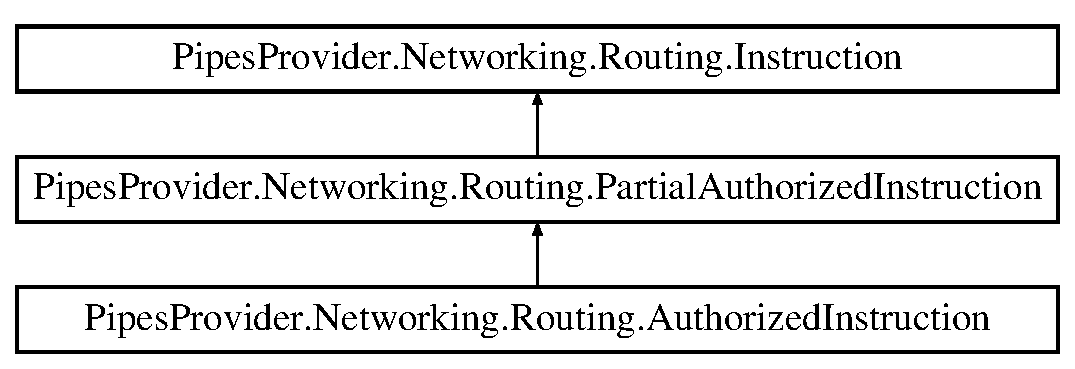
\includegraphics[height=2.000000cm]{df/deb/class_pipes_provider_1_1_networking_1_1_routing_1_1_authorized_instruction}
\end{center}
\end{figure}
\subsection*{Public Member Functions}
\begin{DoxyCompactItemize}
\item 
async void \mbox{\hyperlink{class_pipes_provider_1_1_networking_1_1_routing_1_1_authorized_instruction_a20e94ddf386abb937f4c725a094dc050}{Try\+To\+Logon\+Async}} (System.\+Action$<$ \mbox{\hyperlink{class_pipes_provider_1_1_networking_1_1_routing_1_1_authorized_instruction}{Authorized\+Instruction}} $>$ callback, Cancellation\+Token cancellation\+Token)
\begin{DoxyCompactList}\small\item\em Tring to recive token authorized in authority controller of target server. \end{DoxyCompactList}\item 
bool \mbox{\hyperlink{class_pipes_provider_1_1_networking_1_1_routing_1_1_authorized_instruction_addf69c3fea172cc9d8199097466a052f}{Try\+To\+Logon}} ()
\begin{DoxyCompactList}\small\item\em Tring to recive token authorized in authority controller of target server. \end{DoxyCompactList}\end{DoxyCompactItemize}
\subsection*{Public Attributes}
\begin{DoxyCompactItemize}
\item 
string \mbox{\hyperlink{class_pipes_provider_1_1_networking_1_1_routing_1_1_authorized_instruction_aabef40719c548a28cd3517516be58ded}{auth\+Login}}
\begin{DoxyCompactList}\small\item\em Login for user authentification in \mbox{\hyperlink{namespace_authority_controller}{Authority\+Controller}} on instruction\textquotesingle{}s target server. \end{DoxyCompactList}\item 
string \mbox{\hyperlink{class_pipes_provider_1_1_networking_1_1_routing_1_1_authorized_instruction_aef611c3d3856d276dce814d7f4aaaee2}{auth\+Password}}
\begin{DoxyCompactList}\small\item\em Password for user authentification in \mbox{\hyperlink{namespace_authority_controller}{Authority\+Controller}} on instruction\textquotesingle{}s target server. \end{DoxyCompactList}\item 
string \mbox{\hyperlink{class_pipes_provider_1_1_networking_1_1_routing_1_1_authorized_instruction_a45172a0762b6627107f67e4e7db61780}{guest\+Chanel}} = \char`\"{}guests\char`\"{}
\begin{DoxyCompactList}\small\item\em Name of the broadcasting pipe that providing guest tokens. \end{DoxyCompactList}\end{DoxyCompactItemize}
\subsection*{Properties}
\begin{DoxyCompactItemize}
\item 
string \mbox{\hyperlink{class_pipes_provider_1_1_networking_1_1_routing_1_1_authorized_instruction_a0f856748d300d23a203b5e289007d6fd}{Authorized\+Token}}\hspace{0.3cm}{\ttfamily  \mbox{[}get\mbox{]}}
\begin{DoxyCompactList}\small\item\em Return token authorized on target server by using provided data. \end{DoxyCompactList}\item 
string \mbox{\hyperlink{class_pipes_provider_1_1_networking_1_1_routing_1_1_authorized_instruction_a5bc07dddc515afbe5dc2dcd64c8314ee}{Guest\+Token}}\hspace{0.3cm}{\ttfamily  \mbox{[}get\mbox{]}}
\begin{DoxyCompactList}\small\item\em Return token authorized on target server as guest. \end{DoxyCompactList}\item 
\mbox{\hyperlink{class_authority_controller_1_1_queries_1_1_u_s_e_r___l_o_g_o_n_1_1_logon_processor}{U\+S\+E\+R\+\_\+\+L\+O\+G\+O\+N.\+Logon\+Processor}} \mbox{\hyperlink{class_pipes_provider_1_1_networking_1_1_routing_1_1_authorized_instruction_a9f1721ee3d1fbb3803b77a991f5e1a03}{Logon\+Handler}}\hspace{0.3cm}{\ttfamily  \mbox{[}get\mbox{]}}
\begin{DoxyCompactList}\small\item\em Handler that take full control on logon process. \end{DoxyCompactList}\item 
\mbox{\hyperlink{class_authority_controller_1_1_queries_1_1_g_e_t___g_u_e_s_t___t_o_k_e_n_1_1_guest_token_processor}{G\+E\+T\+\_\+\+G\+U\+E\+S\+T\+\_\+\+T\+O\+K\+E\+N.\+Guest\+Token\+Processor}} \mbox{\hyperlink{class_pipes_provider_1_1_networking_1_1_routing_1_1_authorized_instruction_a69c5e303ece339342c6979ba11436d82}{Guest\+Token\+Handler}}\hspace{0.3cm}{\ttfamily  \mbox{[}get\mbox{]}}
\begin{DoxyCompactList}\small\item\em Handler that take full control on reciving of guest token. \end{DoxyCompactList}\end{DoxyCompactItemize}
\subsection*{Private Attributes}
\begin{DoxyCompactItemize}
\item 
\mbox{\Hypertarget{class_pipes_provider_1_1_networking_1_1_routing_1_1_authorized_instruction_ad4c378226e015ebdcd8390dd63d54669}\label{class_pipes_provider_1_1_networking_1_1_routing_1_1_authorized_instruction_ad4c378226e015ebdcd8390dd63d54669}} 
\mbox{\hyperlink{class_authority_controller_1_1_queries_1_1_u_s_e_r___l_o_g_o_n_1_1_logon_processor}{U\+S\+E\+R\+\_\+\+L\+O\+G\+O\+N.\+Logon\+Processor}} {\bfseries \+\_\+\+Logon\+Handler}
\item 
\mbox{\Hypertarget{class_pipes_provider_1_1_networking_1_1_routing_1_1_authorized_instruction_a981488184cffd1c3f4e91e35bda055ba}\label{class_pipes_provider_1_1_networking_1_1_routing_1_1_authorized_instruction_a981488184cffd1c3f4e91e35bda055ba}} 
\mbox{\hyperlink{class_authority_controller_1_1_queries_1_1_g_e_t___g_u_e_s_t___t_o_k_e_n_1_1_guest_token_processor}{G\+E\+T\+\_\+\+G\+U\+E\+S\+T\+\_\+\+T\+O\+K\+E\+N.\+Guest\+Token\+Processor}} {\bfseries \+\_\+\+Guest\+Token\+Handler}
\end{DoxyCompactItemize}


\subsection{Detailed Description}
Provide data and A\+PI required for connections that require authorization as Authority Controller user. 



\subsection{Member Function Documentation}
\mbox{\Hypertarget{class_pipes_provider_1_1_networking_1_1_routing_1_1_authorized_instruction_addf69c3fea172cc9d8199097466a052f}\label{class_pipes_provider_1_1_networking_1_1_routing_1_1_authorized_instruction_addf69c3fea172cc9d8199097466a052f}} 
\index{Pipes\+Provider\+::\+Networking\+::\+Routing\+::\+Authorized\+Instruction@{Pipes\+Provider\+::\+Networking\+::\+Routing\+::\+Authorized\+Instruction}!Try\+To\+Logon@{Try\+To\+Logon}}
\index{Try\+To\+Logon@{Try\+To\+Logon}!Pipes\+Provider\+::\+Networking\+::\+Routing\+::\+Authorized\+Instruction@{Pipes\+Provider\+::\+Networking\+::\+Routing\+::\+Authorized\+Instruction}}
\subsubsection{\texorpdfstring{Try\+To\+Logon()}{TryToLogon()}}
{\footnotesize\ttfamily bool Pipes\+Provider.\+Networking.\+Routing.\+Authorized\+Instruction.\+Try\+To\+Logon (\begin{DoxyParamCaption}{ }\end{DoxyParamCaption})}



Tring to recive token authorized in authority controller of target server. 

\mbox{\Hypertarget{class_pipes_provider_1_1_networking_1_1_routing_1_1_authorized_instruction_a20e94ddf386abb937f4c725a094dc050}\label{class_pipes_provider_1_1_networking_1_1_routing_1_1_authorized_instruction_a20e94ddf386abb937f4c725a094dc050}} 
\index{Pipes\+Provider\+::\+Networking\+::\+Routing\+::\+Authorized\+Instruction@{Pipes\+Provider\+::\+Networking\+::\+Routing\+::\+Authorized\+Instruction}!Try\+To\+Logon\+Async@{Try\+To\+Logon\+Async}}
\index{Try\+To\+Logon\+Async@{Try\+To\+Logon\+Async}!Pipes\+Provider\+::\+Networking\+::\+Routing\+::\+Authorized\+Instruction@{Pipes\+Provider\+::\+Networking\+::\+Routing\+::\+Authorized\+Instruction}}
\subsubsection{\texorpdfstring{Try\+To\+Logon\+Async()}{TryToLogonAsync()}}
{\footnotesize\ttfamily async void Pipes\+Provider.\+Networking.\+Routing.\+Authorized\+Instruction.\+Try\+To\+Logon\+Async (\begin{DoxyParamCaption}\item[{System.\+Action$<$ \mbox{\hyperlink{class_pipes_provider_1_1_networking_1_1_routing_1_1_authorized_instruction}{Authorized\+Instruction}} $>$}]{callback,  }\item[{Cancellation\+Token}]{cancellation\+Token }\end{DoxyParamCaption})}



Tring to recive token authorized in authority controller of target server. 


\begin{DoxyParams}{Parameters}
{\em callback} & Delegate that will be called when logon operation would be finished.\\
\hline
{\em cancellation\+Token} & Using this token you can terminate task.\\
\hline
\end{DoxyParams}


\subsection{Member Data Documentation}
\mbox{\Hypertarget{class_pipes_provider_1_1_networking_1_1_routing_1_1_authorized_instruction_aabef40719c548a28cd3517516be58ded}\label{class_pipes_provider_1_1_networking_1_1_routing_1_1_authorized_instruction_aabef40719c548a28cd3517516be58ded}} 
\index{Pipes\+Provider\+::\+Networking\+::\+Routing\+::\+Authorized\+Instruction@{Pipes\+Provider\+::\+Networking\+::\+Routing\+::\+Authorized\+Instruction}!auth\+Login@{auth\+Login}}
\index{auth\+Login@{auth\+Login}!Pipes\+Provider\+::\+Networking\+::\+Routing\+::\+Authorized\+Instruction@{Pipes\+Provider\+::\+Networking\+::\+Routing\+::\+Authorized\+Instruction}}
\subsubsection{\texorpdfstring{auth\+Login}{authLogin}}
{\footnotesize\ttfamily string Pipes\+Provider.\+Networking.\+Routing.\+Authorized\+Instruction.\+auth\+Login}



Login for user authentification in \mbox{\hyperlink{namespace_authority_controller}{Authority\+Controller}} on instruction\textquotesingle{}s target server. 

\mbox{\Hypertarget{class_pipes_provider_1_1_networking_1_1_routing_1_1_authorized_instruction_aef611c3d3856d276dce814d7f4aaaee2}\label{class_pipes_provider_1_1_networking_1_1_routing_1_1_authorized_instruction_aef611c3d3856d276dce814d7f4aaaee2}} 
\index{Pipes\+Provider\+::\+Networking\+::\+Routing\+::\+Authorized\+Instruction@{Pipes\+Provider\+::\+Networking\+::\+Routing\+::\+Authorized\+Instruction}!auth\+Password@{auth\+Password}}
\index{auth\+Password@{auth\+Password}!Pipes\+Provider\+::\+Networking\+::\+Routing\+::\+Authorized\+Instruction@{Pipes\+Provider\+::\+Networking\+::\+Routing\+::\+Authorized\+Instruction}}
\subsubsection{\texorpdfstring{auth\+Password}{authPassword}}
{\footnotesize\ttfamily string Pipes\+Provider.\+Networking.\+Routing.\+Authorized\+Instruction.\+auth\+Password}



Password for user authentification in \mbox{\hyperlink{namespace_authority_controller}{Authority\+Controller}} on instruction\textquotesingle{}s target server. 

\mbox{\Hypertarget{class_pipes_provider_1_1_networking_1_1_routing_1_1_authorized_instruction_a45172a0762b6627107f67e4e7db61780}\label{class_pipes_provider_1_1_networking_1_1_routing_1_1_authorized_instruction_a45172a0762b6627107f67e4e7db61780}} 
\index{Pipes\+Provider\+::\+Networking\+::\+Routing\+::\+Authorized\+Instruction@{Pipes\+Provider\+::\+Networking\+::\+Routing\+::\+Authorized\+Instruction}!guest\+Chanel@{guest\+Chanel}}
\index{guest\+Chanel@{guest\+Chanel}!Pipes\+Provider\+::\+Networking\+::\+Routing\+::\+Authorized\+Instruction@{Pipes\+Provider\+::\+Networking\+::\+Routing\+::\+Authorized\+Instruction}}
\subsubsection{\texorpdfstring{guest\+Chanel}{guestChanel}}
{\footnotesize\ttfamily string Pipes\+Provider.\+Networking.\+Routing.\+Authorized\+Instruction.\+guest\+Chanel = \char`\"{}guests\char`\"{}}



Name of the broadcasting pipe that providing guest tokens. 



\subsection{Property Documentation}
\mbox{\Hypertarget{class_pipes_provider_1_1_networking_1_1_routing_1_1_authorized_instruction_a0f856748d300d23a203b5e289007d6fd}\label{class_pipes_provider_1_1_networking_1_1_routing_1_1_authorized_instruction_a0f856748d300d23a203b5e289007d6fd}} 
\index{Pipes\+Provider\+::\+Networking\+::\+Routing\+::\+Authorized\+Instruction@{Pipes\+Provider\+::\+Networking\+::\+Routing\+::\+Authorized\+Instruction}!Authorized\+Token@{Authorized\+Token}}
\index{Authorized\+Token@{Authorized\+Token}!Pipes\+Provider\+::\+Networking\+::\+Routing\+::\+Authorized\+Instruction@{Pipes\+Provider\+::\+Networking\+::\+Routing\+::\+Authorized\+Instruction}}
\subsubsection{\texorpdfstring{Authorized\+Token}{AuthorizedToken}}
{\footnotesize\ttfamily string Pipes\+Provider.\+Networking.\+Routing.\+Authorized\+Instruction.\+Authorized\+Token\hspace{0.3cm}{\ttfamily [get]}}



Return token authorized on target server by using provided data. 

\mbox{\Hypertarget{class_pipes_provider_1_1_networking_1_1_routing_1_1_authorized_instruction_a5bc07dddc515afbe5dc2dcd64c8314ee}\label{class_pipes_provider_1_1_networking_1_1_routing_1_1_authorized_instruction_a5bc07dddc515afbe5dc2dcd64c8314ee}} 
\index{Pipes\+Provider\+::\+Networking\+::\+Routing\+::\+Authorized\+Instruction@{Pipes\+Provider\+::\+Networking\+::\+Routing\+::\+Authorized\+Instruction}!Guest\+Token@{Guest\+Token}}
\index{Guest\+Token@{Guest\+Token}!Pipes\+Provider\+::\+Networking\+::\+Routing\+::\+Authorized\+Instruction@{Pipes\+Provider\+::\+Networking\+::\+Routing\+::\+Authorized\+Instruction}}
\subsubsection{\texorpdfstring{Guest\+Token}{GuestToken}}
{\footnotesize\ttfamily string Pipes\+Provider.\+Networking.\+Routing.\+Authorized\+Instruction.\+Guest\+Token\hspace{0.3cm}{\ttfamily [get]}}



Return token authorized on target server as guest. 

\mbox{\Hypertarget{class_pipes_provider_1_1_networking_1_1_routing_1_1_authorized_instruction_a69c5e303ece339342c6979ba11436d82}\label{class_pipes_provider_1_1_networking_1_1_routing_1_1_authorized_instruction_a69c5e303ece339342c6979ba11436d82}} 
\index{Pipes\+Provider\+::\+Networking\+::\+Routing\+::\+Authorized\+Instruction@{Pipes\+Provider\+::\+Networking\+::\+Routing\+::\+Authorized\+Instruction}!Guest\+Token\+Handler@{Guest\+Token\+Handler}}
\index{Guest\+Token\+Handler@{Guest\+Token\+Handler}!Pipes\+Provider\+::\+Networking\+::\+Routing\+::\+Authorized\+Instruction@{Pipes\+Provider\+::\+Networking\+::\+Routing\+::\+Authorized\+Instruction}}
\subsubsection{\texorpdfstring{Guest\+Token\+Handler}{GuestTokenHandler}}
{\footnotesize\ttfamily \mbox{\hyperlink{class_authority_controller_1_1_queries_1_1_g_e_t___g_u_e_s_t___t_o_k_e_n_1_1_guest_token_processor}{G\+E\+T\+\_\+\+G\+U\+E\+S\+T\+\_\+\+T\+O\+K\+E\+N.\+Guest\+Token\+Processor}} Pipes\+Provider.\+Networking.\+Routing.\+Authorized\+Instruction.\+Guest\+Token\+Handler\hspace{0.3cm}{\ttfamily [get]}, {\ttfamily [private]}}



Handler that take full control on reciving of guest token. 

\mbox{\Hypertarget{class_pipes_provider_1_1_networking_1_1_routing_1_1_authorized_instruction_a9f1721ee3d1fbb3803b77a991f5e1a03}\label{class_pipes_provider_1_1_networking_1_1_routing_1_1_authorized_instruction_a9f1721ee3d1fbb3803b77a991f5e1a03}} 
\index{Pipes\+Provider\+::\+Networking\+::\+Routing\+::\+Authorized\+Instruction@{Pipes\+Provider\+::\+Networking\+::\+Routing\+::\+Authorized\+Instruction}!Logon\+Handler@{Logon\+Handler}}
\index{Logon\+Handler@{Logon\+Handler}!Pipes\+Provider\+::\+Networking\+::\+Routing\+::\+Authorized\+Instruction@{Pipes\+Provider\+::\+Networking\+::\+Routing\+::\+Authorized\+Instruction}}
\subsubsection{\texorpdfstring{Logon\+Handler}{LogonHandler}}
{\footnotesize\ttfamily \mbox{\hyperlink{class_authority_controller_1_1_queries_1_1_u_s_e_r___l_o_g_o_n_1_1_logon_processor}{U\+S\+E\+R\+\_\+\+L\+O\+G\+O\+N.\+Logon\+Processor}} Pipes\+Provider.\+Networking.\+Routing.\+Authorized\+Instruction.\+Logon\+Handler\hspace{0.3cm}{\ttfamily [get]}, {\ttfamily [private]}}



Handler that take full control on logon process. 



The documentation for this class was generated from the following file\+:\begin{DoxyCompactItemize}
\item 
D\+:/\+Work/\+Git\+Hub/doloro-\/networking-\/framework/\+Addons/\+Authority\+Controller/\+Extensions/\+Pipes\+Provider/Authorized\+Instruction.\+cs\end{DoxyCompactItemize}

\hypertarget{class_uniform_queries_1_1_executable_1_1_security_1_1_auth_query_processor}{}\section{Uniform\+Queries.\+Executable.\+Security.\+Auth\+Query\+Processor Class Reference}
\label{class_uniform_queries_1_1_executable_1_1_security_1_1_auth_query_processor}\index{Uniform\+Queries.\+Executable.\+Security.\+Auth\+Query\+Processor@{Uniform\+Queries.\+Executable.\+Security.\+Auth\+Query\+Processor}}


Provide fields situated but authentification queries.  


Inheritance diagram for Uniform\+Queries.\+Executable.\+Security.\+Auth\+Query\+Processor\+:\begin{figure}[H]
\begin{center}
\leavevmode
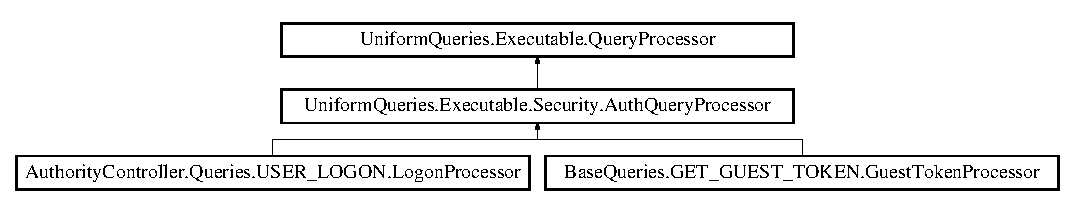
\includegraphics[height=2.326870cm]{dc/d63/class_uniform_queries_1_1_executable_1_1_security_1_1_auth_query_processor}
\end{center}
\end{figure}
\subsection*{Protected Member Functions}
\begin{DoxyCompactItemize}
\item 
override void \mbox{\hyperlink{class_uniform_queries_1_1_executable_1_1_security_1_1_auth_query_processor_a4693289bf81ca5d98fe8f5678a7c4b87}{Server\+Answer\+Handler}} (object \+\_\+, object answer)
\begin{DoxyCompactList}\small\item\em Handler that would recive server answer. \end{DoxyCompactList}\end{DoxyCompactItemize}
\subsection*{Properties}
\begin{DoxyCompactItemize}
\item 
bool \mbox{\hyperlink{class_uniform_queries_1_1_executable_1_1_security_1_1_auth_query_processor_ab77106e3aee595bb89634690bec88d9f}{Is\+Autorized}}\hspace{0.3cm}{\ttfamily  \mbox{[}get, protected set\mbox{]}}
\begin{DoxyCompactList}\small\item\em Check does this instruction authorized. \end{DoxyCompactList}\item 
string \mbox{\hyperlink{class_uniform_queries_1_1_executable_1_1_security_1_1_auth_query_processor_aef3e0af13be8f2e30f3ae95a9e8b58bb}{Token}}\hspace{0.3cm}{\ttfamily  \mbox{[}get, set\mbox{]}}
\begin{DoxyCompactList}\small\item\em Token that would be used during quries to confirm the rights. Logon on target server before using this instruction and save recived token to this property. \end{DoxyCompactList}\item 
System.\+Date\+Time \mbox{\hyperlink{class_uniform_queries_1_1_executable_1_1_security_1_1_auth_query_processor_a09df0334aa792f2b50d90c107d758af4}{Expiry\+Time}}\hspace{0.3cm}{\ttfamily  \mbox{[}get, protected set\mbox{]}}
\begin{DoxyCompactList}\small\item\em Time when token would expited. \end{DoxyCompactList}\item 
string \mbox{[}$\,$\mbox{]} \mbox{\hyperlink{class_uniform_queries_1_1_executable_1_1_security_1_1_auth_query_processor_a29e80b384acdfe7fccfb713a4ae72140}{Recived\+Rights}}\hspace{0.3cm}{\ttfamily  \mbox{[}get, protected set\mbox{]}}
\begin{DoxyCompactList}\small\item\em Rights provided to token during logon. \end{DoxyCompactList}\end{DoxyCompactItemize}
\subsection*{Private Attributes}
\begin{DoxyCompactItemize}
\item 
\mbox{\Hypertarget{class_uniform_queries_1_1_executable_1_1_security_1_1_auth_query_processor_a23b1d7bffb19465106ccb3d27b3df747}\label{class_uniform_queries_1_1_executable_1_1_security_1_1_auth_query_processor_a23b1d7bffb19465106ccb3d27b3df747}} 
bool {\bfseries \+\_\+is\+Autorized}
\item 
\mbox{\Hypertarget{class_uniform_queries_1_1_executable_1_1_security_1_1_auth_query_processor_a8e8ef26ec5dbc22e0d5908254a7cf77b}\label{class_uniform_queries_1_1_executable_1_1_security_1_1_auth_query_processor_a8e8ef26ec5dbc22e0d5908254a7cf77b}} 
string {\bfseries \+\_\+token}
\end{DoxyCompactItemize}
\subsection*{Additional Inherited Members}


\subsection{Detailed Description}
Provide fields situated but authentification queries. 



\subsection{Member Function Documentation}
\mbox{\Hypertarget{class_uniform_queries_1_1_executable_1_1_security_1_1_auth_query_processor_a4693289bf81ca5d98fe8f5678a7c4b87}\label{class_uniform_queries_1_1_executable_1_1_security_1_1_auth_query_processor_a4693289bf81ca5d98fe8f5678a7c4b87}} 
\index{Uniform\+Queries\+::\+Executable\+::\+Security\+::\+Auth\+Query\+Processor@{Uniform\+Queries\+::\+Executable\+::\+Security\+::\+Auth\+Query\+Processor}!Server\+Answer\+Handler@{Server\+Answer\+Handler}}
\index{Server\+Answer\+Handler@{Server\+Answer\+Handler}!Uniform\+Queries\+::\+Executable\+::\+Security\+::\+Auth\+Query\+Processor@{Uniform\+Queries\+::\+Executable\+::\+Security\+::\+Auth\+Query\+Processor}}
\subsubsection{\texorpdfstring{Server\+Answer\+Handler()}{ServerAnswerHandler()}}
{\footnotesize\ttfamily override void Uniform\+Queries.\+Executable.\+Security.\+Auth\+Query\+Processor.\+Server\+Answer\+Handler (\begin{DoxyParamCaption}\item[{object}]{\+\_\+,  }\item[{object}]{answer }\end{DoxyParamCaption})\hspace{0.3cm}{\ttfamily [protected]}, {\ttfamily [virtual]}}



Handler that would recive server answer. 


\begin{DoxyParams}{Parameters}
{\em line} & \\
\hline
{\em answer} & \\
\hline
\end{DoxyParams}


Implements \mbox{\hyperlink{class_uniform_queries_1_1_executable_1_1_query_processor_a4597c1035fc6bb96f9285cb666655a53}{Uniform\+Queries.\+Executable.\+Query\+Processor}}.



\subsection{Property Documentation}
\mbox{\Hypertarget{class_uniform_queries_1_1_executable_1_1_security_1_1_auth_query_processor_a09df0334aa792f2b50d90c107d758af4}\label{class_uniform_queries_1_1_executable_1_1_security_1_1_auth_query_processor_a09df0334aa792f2b50d90c107d758af4}} 
\index{Uniform\+Queries\+::\+Executable\+::\+Security\+::\+Auth\+Query\+Processor@{Uniform\+Queries\+::\+Executable\+::\+Security\+::\+Auth\+Query\+Processor}!Expiry\+Time@{Expiry\+Time}}
\index{Expiry\+Time@{Expiry\+Time}!Uniform\+Queries\+::\+Executable\+::\+Security\+::\+Auth\+Query\+Processor@{Uniform\+Queries\+::\+Executable\+::\+Security\+::\+Auth\+Query\+Processor}}
\subsubsection{\texorpdfstring{Expiry\+Time}{ExpiryTime}}
{\footnotesize\ttfamily System.\+Date\+Time Uniform\+Queries.\+Executable.\+Security.\+Auth\+Query\+Processor.\+Expiry\+Time\hspace{0.3cm}{\ttfamily [get]}, {\ttfamily [protected set]}}



Time when token would expited. 

\mbox{\Hypertarget{class_uniform_queries_1_1_executable_1_1_security_1_1_auth_query_processor_ab77106e3aee595bb89634690bec88d9f}\label{class_uniform_queries_1_1_executable_1_1_security_1_1_auth_query_processor_ab77106e3aee595bb89634690bec88d9f}} 
\index{Uniform\+Queries\+::\+Executable\+::\+Security\+::\+Auth\+Query\+Processor@{Uniform\+Queries\+::\+Executable\+::\+Security\+::\+Auth\+Query\+Processor}!Is\+Autorized@{Is\+Autorized}}
\index{Is\+Autorized@{Is\+Autorized}!Uniform\+Queries\+::\+Executable\+::\+Security\+::\+Auth\+Query\+Processor@{Uniform\+Queries\+::\+Executable\+::\+Security\+::\+Auth\+Query\+Processor}}
\subsubsection{\texorpdfstring{Is\+Autorized}{IsAutorized}}
{\footnotesize\ttfamily bool Uniform\+Queries.\+Executable.\+Security.\+Auth\+Query\+Processor.\+Is\+Autorized\hspace{0.3cm}{\ttfamily [get]}, {\ttfamily [protected set]}}



Check does this instruction authorized. 

\mbox{\Hypertarget{class_uniform_queries_1_1_executable_1_1_security_1_1_auth_query_processor_a29e80b384acdfe7fccfb713a4ae72140}\label{class_uniform_queries_1_1_executable_1_1_security_1_1_auth_query_processor_a29e80b384acdfe7fccfb713a4ae72140}} 
\index{Uniform\+Queries\+::\+Executable\+::\+Security\+::\+Auth\+Query\+Processor@{Uniform\+Queries\+::\+Executable\+::\+Security\+::\+Auth\+Query\+Processor}!Recived\+Rights@{Recived\+Rights}}
\index{Recived\+Rights@{Recived\+Rights}!Uniform\+Queries\+::\+Executable\+::\+Security\+::\+Auth\+Query\+Processor@{Uniform\+Queries\+::\+Executable\+::\+Security\+::\+Auth\+Query\+Processor}}
\subsubsection{\texorpdfstring{Recived\+Rights}{RecivedRights}}
{\footnotesize\ttfamily string \mbox{[}$\,$\mbox{]} Uniform\+Queries.\+Executable.\+Security.\+Auth\+Query\+Processor.\+Recived\+Rights\hspace{0.3cm}{\ttfamily [get]}, {\ttfamily [protected set]}}



Rights provided to token during logon. 

\mbox{\Hypertarget{class_uniform_queries_1_1_executable_1_1_security_1_1_auth_query_processor_aef3e0af13be8f2e30f3ae95a9e8b58bb}\label{class_uniform_queries_1_1_executable_1_1_security_1_1_auth_query_processor_aef3e0af13be8f2e30f3ae95a9e8b58bb}} 
\index{Uniform\+Queries\+::\+Executable\+::\+Security\+::\+Auth\+Query\+Processor@{Uniform\+Queries\+::\+Executable\+::\+Security\+::\+Auth\+Query\+Processor}!Token@{Token}}
\index{Token@{Token}!Uniform\+Queries\+::\+Executable\+::\+Security\+::\+Auth\+Query\+Processor@{Uniform\+Queries\+::\+Executable\+::\+Security\+::\+Auth\+Query\+Processor}}
\subsubsection{\texorpdfstring{Token}{Token}}
{\footnotesize\ttfamily string Uniform\+Queries.\+Executable.\+Security.\+Auth\+Query\+Processor.\+Token\hspace{0.3cm}{\ttfamily [get]}, {\ttfamily [set]}}



Token that would be used during quries to confirm the rights. Logon on target server before using this instruction and save recived token to this property. 



The documentation for this class was generated from the following file\+:\begin{DoxyCompactItemize}
\item 
D\+:/\+Work/\+Git\+Hub/doloro-\/networking-\/framework/\+Core/\+Uniform\+Queries/\+Executable/\+Security/Auth\+Query\+Processor.\+cs\end{DoxyCompactItemize}

\hypertarget{class_authority_controller_1_1_data_1_1_personal_1_1_ban_information}{}\section{Authority\+Controller.\+Data.\+Personal.\+Ban\+Information Class Reference}
\label{class_authority_controller_1_1_data_1_1_personal_1_1_ban_information}\index{Authority\+Controller.\+Data.\+Personal.\+Ban\+Information@{Authority\+Controller.\+Data.\+Personal.\+Ban\+Information}}


Provide information about user bans.  


\subsection*{Public Types}
\begin{DoxyCompactItemize}
\item 
enum \mbox{\hyperlink{class_authority_controller_1_1_data_1_1_personal_1_1_ban_information_a127a28a1db99b43e2540f18949921a7d}{Duration}} \{ {\bfseries Temporary}, 
{\bfseries Permanent}
 \}
\begin{DoxyCompactList}\small\item\em Ban\textquotesingle{}s duration mode. \end{DoxyCompactList}\end{DoxyCompactItemize}
\subsection*{Static Public Member Functions}
\begin{DoxyCompactItemize}
\item 
static bool \mbox{\hyperlink{class_authority_controller_1_1_data_1_1_personal_1_1_ban_information_af71a082c91c5d96b262ccbafe22c821a}{Is\+Banned}} (\mbox{\hyperlink{class_authority_controller_1_1_data_1_1_personal_1_1_user}{User}} user, string right\+Code)
\begin{DoxyCompactList}\small\item\em Check permition for action. \end{DoxyCompactList}\item 
static async Task \mbox{\hyperlink{class_authority_controller_1_1_data_1_1_personal_1_1_ban_information_a70cc71c093fb9f5407b60a88a8361a9b}{Recieve\+Server\+Data\+Async}} (\mbox{\hyperlink{class_authority_controller_1_1_data_1_1_personal_1_1_user}{User}} user, System.\+Action$<$ \mbox{\hyperlink{class_authority_controller_1_1_data_1_1_personal_1_1_ban_information}{Ban\+Information}} $>$ callback)
\begin{DoxyCompactList}\small\item\em Recieving data from connected S\+QL server based on user profile meta. \end{DoxyCompactList}\end{DoxyCompactItemize}
\subsection*{Public Attributes}
\begin{DoxyCompactItemize}
\item 
int \mbox{\hyperlink{class_authority_controller_1_1_data_1_1_personal_1_1_ban_information_a723ebbe0f1de9d495ddc1415fbe8d58d}{id}} = -\/1
\begin{DoxyCompactList}\small\item\em Unique identifier of this ban. \end{DoxyCompactList}\item 
uint \mbox{\hyperlink{class_authority_controller_1_1_data_1_1_personal_1_1_ban_information_a1a674fa4493f3392a4726854e0316607}{user\+Id}} = 0
\begin{DoxyCompactList}\small\item\em Id of banned user. \end{DoxyCompactList}\item 
uint \mbox{\hyperlink{class_authority_controller_1_1_data_1_1_personal_1_1_ban_information_acdff2dd2a45cde1adf6586e631c99916}{banned\+By\+User\+Id}} = 0
\begin{DoxyCompactList}\small\item\em Id of user who signed ban. \end{DoxyCompactList}\item 
bool \mbox{\hyperlink{class_authority_controller_1_1_data_1_1_personal_1_1_ban_information_a8aa7fea19a5b2acce008883fcda629b2}{active}}
\begin{DoxyCompactList}\small\item\em If ban is active? \end{DoxyCompactList}\item 
\mbox{\hyperlink{class_authority_controller_1_1_data_1_1_personal_1_1_ban_information_a127a28a1db99b43e2540f18949921a7d}{Duration}} \mbox{\hyperlink{class_authority_controller_1_1_data_1_1_personal_1_1_ban_information_a68241c910c08c5659c1fcbc86e9ee8a8}{duration}}
\begin{DoxyCompactList}\small\item\em Duration mode of this ban. \end{DoxyCompactList}\item 
Date\+Time \mbox{\hyperlink{class_authority_controller_1_1_data_1_1_personal_1_1_ban_information_ac999bc7a08b0ac597e37898a74c3d79b}{expiry\+Time}}
\begin{DoxyCompactList}\small\item\em Date Time when this bun will be expired. \end{DoxyCompactList}\item 
string \mbox{\hyperlink{class_authority_controller_1_1_data_1_1_personal_1_1_ban_information_a4b408f380448e918f8915510aaf4c159}{commentary}}
\begin{DoxyCompactList}\small\item\em Resones for ban. \end{DoxyCompactList}\item 
string \mbox{[}$\,$\mbox{]} \mbox{\hyperlink{class_authority_controller_1_1_data_1_1_personal_1_1_ban_information_a3bfad0aa4906e8e60de00e93e4ee52a8}{blocked\+Rights}}
\begin{DoxyCompactList}\small\item\em Rights that was blocked for this user. \end{DoxyCompactList}\end{DoxyCompactItemize}
\subsection*{Properties}
\begin{DoxyCompactItemize}
\item 
static \mbox{\hyperlink{class_authority_controller_1_1_data_1_1_personal_1_1_ban_information}{Ban\+Information}} \mbox{\hyperlink{class_authority_controller_1_1_data_1_1_personal_1_1_ban_information_a129ecfe581f8d778a6b71cd13b7e8b77}{Permanent}}\hspace{0.3cm}{\ttfamily  \mbox{[}get\mbox{]}}
\begin{DoxyCompactList}\small\item\em Return information for permanent ban. \end{DoxyCompactList}\item 
int \mbox{\hyperlink{class_authority_controller_1_1_data_1_1_personal_1_1_ban_information_ac4ff6168fd023122851068927068178f}{Duration\+Int}}\hspace{0.3cm}{\ttfamily  \mbox{[}get, set\mbox{]}}
\begin{DoxyCompactList}\small\item\em Duration in int format that can be stored to the S\+QL server. \end{DoxyCompactList}\item 
byte \mbox{[}$\,$\mbox{]} \mbox{\hyperlink{class_authority_controller_1_1_data_1_1_personal_1_1_ban_information_a6bbdcde258fbc08ded3d2c6d022767f7}{Blocked\+Rights\+Blob}}\hspace{0.3cm}{\ttfamily  \mbox{[}get, set\mbox{]}}
\begin{DoxyCompactList}\small\item\em Blocked rights array in binnary format. \end{DoxyCompactList}\item 
bool \mbox{\hyperlink{class_authority_controller_1_1_data_1_1_personal_1_1_ban_information_ad07cbe220f0625c0b22183d764709d74}{Is\+Expired}}\hspace{0.3cm}{\ttfamily  \mbox{[}get\mbox{]}}
\begin{DoxyCompactList}\small\item\em Check is this ban still actual. \end{DoxyCompactList}\end{DoxyCompactItemize}


\subsection{Detailed Description}
Provide information about user bans. 



\subsection{Member Enumeration Documentation}
\mbox{\Hypertarget{class_authority_controller_1_1_data_1_1_personal_1_1_ban_information_a127a28a1db99b43e2540f18949921a7d}\label{class_authority_controller_1_1_data_1_1_personal_1_1_ban_information_a127a28a1db99b43e2540f18949921a7d}} 
\index{Authority\+Controller\+::\+Data\+::\+Personal\+::\+Ban\+Information@{Authority\+Controller\+::\+Data\+::\+Personal\+::\+Ban\+Information}!Duration@{Duration}}
\index{Duration@{Duration}!Authority\+Controller\+::\+Data\+::\+Personal\+::\+Ban\+Information@{Authority\+Controller\+::\+Data\+::\+Personal\+::\+Ban\+Information}}
\subsubsection{\texorpdfstring{Duration}{Duration}}
{\footnotesize\ttfamily enum \mbox{\hyperlink{class_authority_controller_1_1_data_1_1_personal_1_1_ban_information_a127a28a1db99b43e2540f18949921a7d}{Authority\+Controller.\+Data.\+Personal.\+Ban\+Information.\+Duration}}\hspace{0.3cm}{\ttfamily [strong]}}



Ban\textquotesingle{}s duration mode. 



\subsection{Member Function Documentation}
\mbox{\Hypertarget{class_authority_controller_1_1_data_1_1_personal_1_1_ban_information_af71a082c91c5d96b262ccbafe22c821a}\label{class_authority_controller_1_1_data_1_1_personal_1_1_ban_information_af71a082c91c5d96b262ccbafe22c821a}} 
\index{Authority\+Controller\+::\+Data\+::\+Personal\+::\+Ban\+Information@{Authority\+Controller\+::\+Data\+::\+Personal\+::\+Ban\+Information}!Is\+Banned@{Is\+Banned}}
\index{Is\+Banned@{Is\+Banned}!Authority\+Controller\+::\+Data\+::\+Personal\+::\+Ban\+Information@{Authority\+Controller\+::\+Data\+::\+Personal\+::\+Ban\+Information}}
\subsubsection{\texorpdfstring{Is\+Banned()}{IsBanned()}}
{\footnotesize\ttfamily static bool Authority\+Controller.\+Data.\+Personal.\+Ban\+Information.\+Is\+Banned (\begin{DoxyParamCaption}\item[{\mbox{\hyperlink{class_authority_controller_1_1_data_1_1_personal_1_1_user}{User}}}]{user,  }\item[{string}]{right\+Code }\end{DoxyParamCaption})\hspace{0.3cm}{\ttfamily [static]}}



Check permition for action. 


\begin{DoxyParams}{Parameters}
{\em user} & Target user.\\
\hline
{\em right\+Code} & Code of right that required for action.\\
\hline
\end{DoxyParams}
\begin{DoxyReturn}{Returns}

\end{DoxyReturn}
\mbox{\Hypertarget{class_authority_controller_1_1_data_1_1_personal_1_1_ban_information_a70cc71c093fb9f5407b60a88a8361a9b}\label{class_authority_controller_1_1_data_1_1_personal_1_1_ban_information_a70cc71c093fb9f5407b60a88a8361a9b}} 
\index{Authority\+Controller\+::\+Data\+::\+Personal\+::\+Ban\+Information@{Authority\+Controller\+::\+Data\+::\+Personal\+::\+Ban\+Information}!Recieve\+Server\+Data\+Async@{Recieve\+Server\+Data\+Async}}
\index{Recieve\+Server\+Data\+Async@{Recieve\+Server\+Data\+Async}!Authority\+Controller\+::\+Data\+::\+Personal\+::\+Ban\+Information@{Authority\+Controller\+::\+Data\+::\+Personal\+::\+Ban\+Information}}
\subsubsection{\texorpdfstring{Recieve\+Server\+Data\+Async()}{RecieveServerDataAsync()}}
{\footnotesize\ttfamily static async Task Authority\+Controller.\+Data.\+Personal.\+Ban\+Information.\+Recieve\+Server\+Data\+Async (\begin{DoxyParamCaption}\item[{\mbox{\hyperlink{class_authority_controller_1_1_data_1_1_personal_1_1_user}{User}}}]{user,  }\item[{System.\+Action$<$ \mbox{\hyperlink{class_authority_controller_1_1_data_1_1_personal_1_1_ban_information}{Ban\+Information}} $>$}]{callback }\end{DoxyParamCaption})\hspace{0.3cm}{\ttfamily [static]}}



Recieving data from connected S\+QL server based on user profile meta. 


\begin{DoxyParams}{Parameters}
{\em user} & Profile that contains core meta like id, login, etc.\\
\hline
{\em callback} & Delegate that would be called after finishing of operation. Return ban information. Null if not exist or failed.\\
\hline
\end{DoxyParams}
\begin{DoxyReturn}{Returns}

\end{DoxyReturn}


\subsection{Member Data Documentation}
\mbox{\Hypertarget{class_authority_controller_1_1_data_1_1_personal_1_1_ban_information_a8aa7fea19a5b2acce008883fcda629b2}\label{class_authority_controller_1_1_data_1_1_personal_1_1_ban_information_a8aa7fea19a5b2acce008883fcda629b2}} 
\index{Authority\+Controller\+::\+Data\+::\+Personal\+::\+Ban\+Information@{Authority\+Controller\+::\+Data\+::\+Personal\+::\+Ban\+Information}!active@{active}}
\index{active@{active}!Authority\+Controller\+::\+Data\+::\+Personal\+::\+Ban\+Information@{Authority\+Controller\+::\+Data\+::\+Personal\+::\+Ban\+Information}}
\subsubsection{\texorpdfstring{active}{active}}
{\footnotesize\ttfamily bool Authority\+Controller.\+Data.\+Personal.\+Ban\+Information.\+active}



If ban is active? 

\mbox{\Hypertarget{class_authority_controller_1_1_data_1_1_personal_1_1_ban_information_acdff2dd2a45cde1adf6586e631c99916}\label{class_authority_controller_1_1_data_1_1_personal_1_1_ban_information_acdff2dd2a45cde1adf6586e631c99916}} 
\index{Authority\+Controller\+::\+Data\+::\+Personal\+::\+Ban\+Information@{Authority\+Controller\+::\+Data\+::\+Personal\+::\+Ban\+Information}!banned\+By\+User\+Id@{banned\+By\+User\+Id}}
\index{banned\+By\+User\+Id@{banned\+By\+User\+Id}!Authority\+Controller\+::\+Data\+::\+Personal\+::\+Ban\+Information@{Authority\+Controller\+::\+Data\+::\+Personal\+::\+Ban\+Information}}
\subsubsection{\texorpdfstring{banned\+By\+User\+Id}{bannedByUserId}}
{\footnotesize\ttfamily uint Authority\+Controller.\+Data.\+Personal.\+Ban\+Information.\+banned\+By\+User\+Id = 0}



Id of user who signed ban. 

\mbox{\Hypertarget{class_authority_controller_1_1_data_1_1_personal_1_1_ban_information_a3bfad0aa4906e8e60de00e93e4ee52a8}\label{class_authority_controller_1_1_data_1_1_personal_1_1_ban_information_a3bfad0aa4906e8e60de00e93e4ee52a8}} 
\index{Authority\+Controller\+::\+Data\+::\+Personal\+::\+Ban\+Information@{Authority\+Controller\+::\+Data\+::\+Personal\+::\+Ban\+Information}!blocked\+Rights@{blocked\+Rights}}
\index{blocked\+Rights@{blocked\+Rights}!Authority\+Controller\+::\+Data\+::\+Personal\+::\+Ban\+Information@{Authority\+Controller\+::\+Data\+::\+Personal\+::\+Ban\+Information}}
\subsubsection{\texorpdfstring{blocked\+Rights}{blockedRights}}
{\footnotesize\ttfamily string \mbox{[}$\,$\mbox{]} Authority\+Controller.\+Data.\+Personal.\+Ban\+Information.\+blocked\+Rights}



Rights that was blocked for this user. 

Recommend\+: logon -\/ block possibility to logon. commenting -\/ block possibility to post commentaries. etc. \mbox{\Hypertarget{class_authority_controller_1_1_data_1_1_personal_1_1_ban_information_a4b408f380448e918f8915510aaf4c159}\label{class_authority_controller_1_1_data_1_1_personal_1_1_ban_information_a4b408f380448e918f8915510aaf4c159}} 
\index{Authority\+Controller\+::\+Data\+::\+Personal\+::\+Ban\+Information@{Authority\+Controller\+::\+Data\+::\+Personal\+::\+Ban\+Information}!commentary@{commentary}}
\index{commentary@{commentary}!Authority\+Controller\+::\+Data\+::\+Personal\+::\+Ban\+Information@{Authority\+Controller\+::\+Data\+::\+Personal\+::\+Ban\+Information}}
\subsubsection{\texorpdfstring{commentary}{commentary}}
{\footnotesize\ttfamily string Authority\+Controller.\+Data.\+Personal.\+Ban\+Information.\+commentary}



Resones for ban. 

\mbox{\Hypertarget{class_authority_controller_1_1_data_1_1_personal_1_1_ban_information_a68241c910c08c5659c1fcbc86e9ee8a8}\label{class_authority_controller_1_1_data_1_1_personal_1_1_ban_information_a68241c910c08c5659c1fcbc86e9ee8a8}} 
\index{Authority\+Controller\+::\+Data\+::\+Personal\+::\+Ban\+Information@{Authority\+Controller\+::\+Data\+::\+Personal\+::\+Ban\+Information}!duration@{duration}}
\index{duration@{duration}!Authority\+Controller\+::\+Data\+::\+Personal\+::\+Ban\+Information@{Authority\+Controller\+::\+Data\+::\+Personal\+::\+Ban\+Information}}
\subsubsection{\texorpdfstring{duration}{duration}}
{\footnotesize\ttfamily \mbox{\hyperlink{class_authority_controller_1_1_data_1_1_personal_1_1_ban_information_a127a28a1db99b43e2540f18949921a7d}{Duration}} Authority\+Controller.\+Data.\+Personal.\+Ban\+Information.\+duration}



Duration mode of this ban. 

Permanent will no have expiry time. \mbox{\Hypertarget{class_authority_controller_1_1_data_1_1_personal_1_1_ban_information_ac999bc7a08b0ac597e37898a74c3d79b}\label{class_authority_controller_1_1_data_1_1_personal_1_1_ban_information_ac999bc7a08b0ac597e37898a74c3d79b}} 
\index{Authority\+Controller\+::\+Data\+::\+Personal\+::\+Ban\+Information@{Authority\+Controller\+::\+Data\+::\+Personal\+::\+Ban\+Information}!expiry\+Time@{expiry\+Time}}
\index{expiry\+Time@{expiry\+Time}!Authority\+Controller\+::\+Data\+::\+Personal\+::\+Ban\+Information@{Authority\+Controller\+::\+Data\+::\+Personal\+::\+Ban\+Information}}
\subsubsection{\texorpdfstring{expiry\+Time}{expiryTime}}
{\footnotesize\ttfamily Date\+Time Authority\+Controller.\+Data.\+Personal.\+Ban\+Information.\+expiry\+Time}



Date Time when this bun will be expired. 

\mbox{\Hypertarget{class_authority_controller_1_1_data_1_1_personal_1_1_ban_information_a723ebbe0f1de9d495ddc1415fbe8d58d}\label{class_authority_controller_1_1_data_1_1_personal_1_1_ban_information_a723ebbe0f1de9d495ddc1415fbe8d58d}} 
\index{Authority\+Controller\+::\+Data\+::\+Personal\+::\+Ban\+Information@{Authority\+Controller\+::\+Data\+::\+Personal\+::\+Ban\+Information}!id@{id}}
\index{id@{id}!Authority\+Controller\+::\+Data\+::\+Personal\+::\+Ban\+Information@{Authority\+Controller\+::\+Data\+::\+Personal\+::\+Ban\+Information}}
\subsubsection{\texorpdfstring{id}{id}}
{\footnotesize\ttfamily int Authority\+Controller.\+Data.\+Personal.\+Ban\+Information.\+id = -\/1}



Unique identifier of this ban. 

\mbox{\Hypertarget{class_authority_controller_1_1_data_1_1_personal_1_1_ban_information_a1a674fa4493f3392a4726854e0316607}\label{class_authority_controller_1_1_data_1_1_personal_1_1_ban_information_a1a674fa4493f3392a4726854e0316607}} 
\index{Authority\+Controller\+::\+Data\+::\+Personal\+::\+Ban\+Information@{Authority\+Controller\+::\+Data\+::\+Personal\+::\+Ban\+Information}!user\+Id@{user\+Id}}
\index{user\+Id@{user\+Id}!Authority\+Controller\+::\+Data\+::\+Personal\+::\+Ban\+Information@{Authority\+Controller\+::\+Data\+::\+Personal\+::\+Ban\+Information}}
\subsubsection{\texorpdfstring{user\+Id}{userId}}
{\footnotesize\ttfamily uint Authority\+Controller.\+Data.\+Personal.\+Ban\+Information.\+user\+Id = 0}



Id of banned user. 



\subsection{Property Documentation}
\mbox{\Hypertarget{class_authority_controller_1_1_data_1_1_personal_1_1_ban_information_a6bbdcde258fbc08ded3d2c6d022767f7}\label{class_authority_controller_1_1_data_1_1_personal_1_1_ban_information_a6bbdcde258fbc08ded3d2c6d022767f7}} 
\index{Authority\+Controller\+::\+Data\+::\+Personal\+::\+Ban\+Information@{Authority\+Controller\+::\+Data\+::\+Personal\+::\+Ban\+Information}!Blocked\+Rights\+Blob@{Blocked\+Rights\+Blob}}
\index{Blocked\+Rights\+Blob@{Blocked\+Rights\+Blob}!Authority\+Controller\+::\+Data\+::\+Personal\+::\+Ban\+Information@{Authority\+Controller\+::\+Data\+::\+Personal\+::\+Ban\+Information}}
\subsubsection{\texorpdfstring{Blocked\+Rights\+Blob}{BlockedRightsBlob}}
{\footnotesize\ttfamily byte \mbox{[}$\,$\mbox{]} Authority\+Controller.\+Data.\+Personal.\+Ban\+Information.\+Blocked\+Rights\+Blob\hspace{0.3cm}{\ttfamily [get]}, {\ttfamily [set]}}



Blocked rights array in binnary format. 

\mbox{\Hypertarget{class_authority_controller_1_1_data_1_1_personal_1_1_ban_information_ac4ff6168fd023122851068927068178f}\label{class_authority_controller_1_1_data_1_1_personal_1_1_ban_information_ac4ff6168fd023122851068927068178f}} 
\index{Authority\+Controller\+::\+Data\+::\+Personal\+::\+Ban\+Information@{Authority\+Controller\+::\+Data\+::\+Personal\+::\+Ban\+Information}!Duration\+Int@{Duration\+Int}}
\index{Duration\+Int@{Duration\+Int}!Authority\+Controller\+::\+Data\+::\+Personal\+::\+Ban\+Information@{Authority\+Controller\+::\+Data\+::\+Personal\+::\+Ban\+Information}}
\subsubsection{\texorpdfstring{Duration\+Int}{DurationInt}}
{\footnotesize\ttfamily int Authority\+Controller.\+Data.\+Personal.\+Ban\+Information.\+Duration\+Int\hspace{0.3cm}{\ttfamily [get]}, {\ttfamily [set]}}



Duration in int format that can be stored to the S\+QL server. 

\mbox{\Hypertarget{class_authority_controller_1_1_data_1_1_personal_1_1_ban_information_ad07cbe220f0625c0b22183d764709d74}\label{class_authority_controller_1_1_data_1_1_personal_1_1_ban_information_ad07cbe220f0625c0b22183d764709d74}} 
\index{Authority\+Controller\+::\+Data\+::\+Personal\+::\+Ban\+Information@{Authority\+Controller\+::\+Data\+::\+Personal\+::\+Ban\+Information}!Is\+Expired@{Is\+Expired}}
\index{Is\+Expired@{Is\+Expired}!Authority\+Controller\+::\+Data\+::\+Personal\+::\+Ban\+Information@{Authority\+Controller\+::\+Data\+::\+Personal\+::\+Ban\+Information}}
\subsubsection{\texorpdfstring{Is\+Expired}{IsExpired}}
{\footnotesize\ttfamily bool Authority\+Controller.\+Data.\+Personal.\+Ban\+Information.\+Is\+Expired\hspace{0.3cm}{\ttfamily [get]}}



Check is this ban still actual. 

\begin{DoxyReturn}{Returns}

\end{DoxyReturn}
\mbox{\Hypertarget{class_authority_controller_1_1_data_1_1_personal_1_1_ban_information_a129ecfe581f8d778a6b71cd13b7e8b77}\label{class_authority_controller_1_1_data_1_1_personal_1_1_ban_information_a129ecfe581f8d778a6b71cd13b7e8b77}} 
\index{Authority\+Controller\+::\+Data\+::\+Personal\+::\+Ban\+Information@{Authority\+Controller\+::\+Data\+::\+Personal\+::\+Ban\+Information}!Permanent@{Permanent}}
\index{Permanent@{Permanent}!Authority\+Controller\+::\+Data\+::\+Personal\+::\+Ban\+Information@{Authority\+Controller\+::\+Data\+::\+Personal\+::\+Ban\+Information}}
\subsubsection{\texorpdfstring{Permanent}{Permanent}}
{\footnotesize\ttfamily \mbox{\hyperlink{class_authority_controller_1_1_data_1_1_personal_1_1_ban_information}{Ban\+Information}} Authority\+Controller.\+Data.\+Personal.\+Ban\+Information.\+Permanent\hspace{0.3cm}{\ttfamily [static]}, {\ttfamily [get]}}



Return information for permanent ban. 



The documentation for this class was generated from the following file\+:\begin{DoxyCompactItemize}
\item 
D\+:/\+Work/\+Git\+Hub/doloro-\/networking-\/framework/\+Addons/\+Authority\+Controller/\+Data/\+Personal/Ban\+Information.\+cs\end{DoxyCompactItemize}

\hypertarget{class_uniform_client_1_1_base_client}{}\section{Uniform\+Client.\+Base\+Client Class Reference}
\label{class_uniform_client_1_1_base_client}\index{Uniform\+Client.\+Base\+Client@{Uniform\+Client.\+Base\+Client}}


Class that provide base client features and envirounment static A\+PI.  


Inheritance diagram for Uniform\+Client.\+Base\+Client\+:\begin{figure}[H]
\begin{center}
\leavevmode
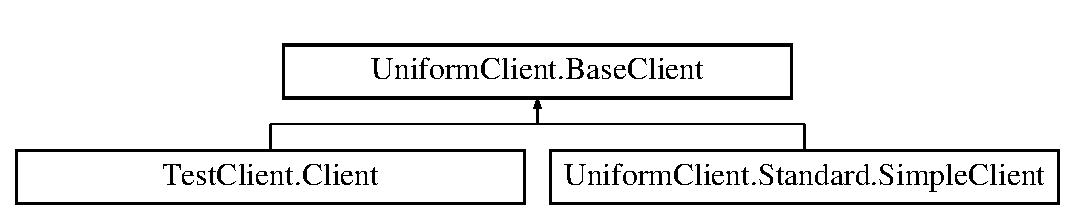
\includegraphics[height=2.000000cm]{d4/deb/class_uniform_client_1_1_base_client}
\end{center}
\end{figure}
\subsection*{Static Public Member Functions}
\begin{DoxyCompactItemize}
\item 
static System.\+Collections.\+Generic.\+I\+Enumerable$<$ \mbox{\hyperlink{interface_uniform_client_1_1_plugins_1_1_i_plugin}{Plugins.\+I\+Plugin}} $>$ \mbox{\hyperlink{class_uniform_client_1_1_base_client_aa60dbfa5bd8c46659aec7738193315f1}{Load\+Plugins\+Enumerable}} ()
\begin{DoxyCompactList}\small\item\em Load plugins from assembly and instiniate them to list. \end{DoxyCompactList}\item 
static System.\+Collections.\+Object\+Model.\+Observable\+Collection$<$ \mbox{\hyperlink{interface_uniform_client_1_1_plugins_1_1_i_plugin}{Plugins.\+I\+Plugin}} $>$ \mbox{\hyperlink{class_uniform_client_1_1_base_client_a99ae0bb1dd5bef374fcedb3f873bfe8b}{Load\+Plugins\+Collection}} ()
\begin{DoxyCompactList}\small\item\em Load plugins from assembly and instiniate them to list. \end{DoxyCompactList}\item 
static R\+S\+A\+Parameters \mbox{\hyperlink{class_uniform_client_1_1_base_client_a849e820e6135840e615b759cb09cd2dd}{Get\+Valid\+Public\+Key\+Via\+PP}} (\mbox{\hyperlink{class_pipes_provider_1_1_networking_1_1_routing_1_1_instruction}{Pipes\+Provider.\+Networking.\+Routing.\+Instruction}} instruction)
\begin{DoxyCompactList}\small\item\em Provide valid public key for target server encryption. Auto update key if was expired. \end{DoxyCompactList}\item 
static async void \mbox{\hyperlink{class_uniform_client_1_1_base_client_a8b0bf0f5c032239a7b1bdc73d2d5ad3d}{Handler\+Input\+Transmission\+Async}} (object shared\+Object)
\begin{DoxyCompactList}\small\item\em Handler that will recive message from the server. \end{DoxyCompactList}\item 
static async void \mbox{\hyperlink{class_uniform_client_1_1_base_client_a233b9fc7f1cdc4df399115938afd917d}{Handler\+Output\+Transmisssion\+Async}} (object shared\+Object)
\begin{DoxyCompactList}\small\item\em Handler that send last dequeued query to server when connection will be established. \end{DoxyCompactList}\item 
static \mbox{\hyperlink{class_pipes_provider_1_1_client_1_1_transmission_line}{Transmission\+Line}} \mbox{\hyperlink{class_uniform_client_1_1_base_client_a56ba8d0360e3c65a69d2d69db878ec23}{Open\+Out\+Transmission\+Line\+Via\+PP}} (string server\+Name, string pipe\+Name)
\begin{DoxyCompactList}\small\item\em Oppening transmition line that will able to send querie to described server\textquotesingle{}s pipe. \end{DoxyCompactList}\item 
static bool \mbox{\hyperlink{class_uniform_client_1_1_base_client_aa6a13dcf0a4dbefd681cf7eb333813aa}{Receive\+Delayed\+Answer\+Via\+PP}} (\mbox{\hyperlink{class_pipes_provider_1_1_client_1_1_transmission_line}{Transmission\+Line}} line, string decoded\+Query, System.\+Action$<$ \mbox{\hyperlink{class_pipes_provider_1_1_client_1_1_transmission_line}{Transmission\+Line}}, object $>$ answer\+Handler)
\begin{DoxyCompactList}\small\item\em Open a line that will be ready to recive server answer. New line will created related to params of requesting line and sended query. \end{DoxyCompactList}\item 
static bool \mbox{\hyperlink{class_uniform_client_1_1_base_client_a4db768d7c09862ab9adc9d7b0638edc6}{Receive\+Delayed\+Answer\+Via\+PP}} (\mbox{\hyperlink{class_pipes_provider_1_1_client_1_1_transmission_line}{Transmission\+Line}} line, \mbox{\hyperlink{struct_uniform_queries_1_1_query_part}{Uniform\+Queries.\+Query\+Part}}\mbox{[}$\,$\mbox{]} entry\+Query\+Parts, System.\+Action$<$ \mbox{\hyperlink{class_pipes_provider_1_1_client_1_1_transmission_line}{Transmission\+Line}}, object $>$ answer\+Handler)
\begin{DoxyCompactList}\small\item\em Open a line that will be ready to recive server answer. New line will created related to params of requesting line and sended query. \end{DoxyCompactList}\item 
static \mbox{\hyperlink{class_pipes_provider_1_1_client_1_1_transmission_line}{Transmission\+Line}} \mbox{\hyperlink{class_uniform_client_1_1_base_client_a97a86c4f5931d39e09ce7c9d336a1636}{Recive\+Anonymous\+Broadcast\+Message}} (string server\+Name, string pipe\+Name, System.\+Action$<$ \mbox{\hyperlink{class_pipes_provider_1_1_client_1_1_transmission_line}{Transmission\+Line}}, object $>$ answer\+Handler)
\begin{DoxyCompactList}\small\item\em Recive message from broadcasting server. A\+T\+T\+E\+N\+T\+I\+ON\+: Eould connect to server as guest user. \end{DoxyCompactList}\item 
static void \mbox{\hyperlink{class_uniform_client_1_1_base_client_a964bd521f46fd99f64b10257c5d233ef}{Enqueue\+Duplex\+Query\+Via\+PP}} (\mbox{\hyperlink{class_pipes_provider_1_1_client_1_1_transmission_line}{Transmission\+Line}} line, string query, System.\+Action$<$ \mbox{\hyperlink{class_pipes_provider_1_1_client_1_1_transmission_line}{Transmission\+Line}}, object $>$ answer\+Handler)
\begin{DoxyCompactList}\small\item\em Add query to queue. Open backward line that will call answer handler. \end{DoxyCompactList}\item 
static \mbox{\hyperlink{class_pipes_provider_1_1_client_1_1_transmission_line}{Transmission\+Line}} \mbox{\hyperlink{class_uniform_client_1_1_base_client_a82dbf660ec06b5c05730ff57b63b4f28}{Enqueue\+Duplex\+Query\+Via\+PP}} (string server\+Name, string server\+Pipe\+Name, string query, System.\+Action$<$ \mbox{\hyperlink{class_pipes_provider_1_1_client_1_1_transmission_line}{Transmission\+Line}}, object $>$ answer\+Handler)
\begin{DoxyCompactList}\small\item\em Add query to queue. Open backward line that will call answer handler. \end{DoxyCompactList}\item 
static void \mbox{\hyperlink{class_uniform_client_1_1_base_client_a5f8f22aa4ab8219fb5f1b6a358f68daf}{Load\+Routing\+Tables}} (params string\mbox{[}$\,$\mbox{]} directories)
\begin{DoxyCompactList}\small\item\em Update routing table by the files that will found be requested directory. Also auto loking for core routing table by \char`\"{}resources\textbackslash{}routing\textbackslash{}\char`\"{}. \end{DoxyCompactList}\item 
static \mbox{\hyperlink{class_pipes_provider_1_1_client_1_1_transmission_line}{Transmission\+Line}} \mbox{\hyperlink{class_uniform_client_1_1_base_client_a851ce49c50011eb0ed2552663c7731ab}{Open\+Transmission\+Line\+Via\+PP}} (string server\+Name, string pipe\+Name, System.\+Action$<$ \mbox{\hyperlink{class_pipes_provider_1_1_client_1_1_transmission_line}{Transmission\+Line}} $>$ callback)
\begin{DoxyCompactList}\small\item\em Automaticly create Transmission line or lokking for previos one. \end{DoxyCompactList}\item 
static \mbox{\hyperlink{class_pipes_provider_1_1_client_1_1_transmission_line}{Transmission\+Line}} \mbox{\hyperlink{class_uniform_client_1_1_base_client_a79c6e490b20b4b8c649af33926e20017}{Open\+Transmission\+Line\+Via\+PP}} (\mbox{\hyperlink{class_uniform_client_1_1_base_client}{Base\+Client}} client, string server\+Name, string pipe\+Name, ref Safe\+Access\+Token\+Handle \mbox{\hyperlink{class_uniform_client_1_1_base_client_ad99bcf3d1afeed6eadca7035c926d2b7}{token}}, System.\+Action$<$ \mbox{\hyperlink{class_pipes_provider_1_1_client_1_1_transmission_line}{Transmission\+Line}} $>$ callback)
\begin{DoxyCompactList}\small\item\em Provide complex initalization of all relative systems. Build meta data, regitrate line in common table. Start new thread to avoid freezes. \end{DoxyCompactList}\end{DoxyCompactItemize}
\subsection*{Public Attributes}
\begin{DoxyCompactItemize}
\item 
Thread \mbox{\hyperlink{class_uniform_client_1_1_base_client_a458271823ca5e21612c0947e1db695a0}{thread}}
\begin{DoxyCompactList}\small\item\em Reference to thread that host this server. \end{DoxyCompactList}\end{DoxyCompactItemize}
\subsection*{Static Public Attributes}
\begin{DoxyCompactItemize}
\item 
static string \mbox{\hyperlink{class_uniform_client_1_1_base_client_ad99bcf3d1afeed6eadca7035c926d2b7}{token}}
\begin{DoxyCompactList}\small\item\em Token that authorize client to data and commands access. \end{DoxyCompactList}\item 
static \mbox{\hyperlink{class_pipes_provider_1_1_networking_1_1_routing_1_1_routing_table}{Routing\+Table}} \mbox{\hyperlink{class_uniform_client_1_1_base_client_a33b34ea9a2d7b4b8e26af767ab2897cf}{routing\+Table}}
\begin{DoxyCompactList}\small\item\em Table that contain instruction that allow to determine the server which is a target for recived query. \end{DoxyCompactList}\end{DoxyCompactItemize}
\subsection*{Protected Member Functions}
\begin{DoxyCompactItemize}
\item 
virtual Thread \mbox{\hyperlink{class_uniform_client_1_1_base_client_a194b46bb0e889d07cade81c0aeab7cea}{Start\+Client\+Thread}} (string thread\+Name, object shareble\+Param, Parameterized\+Thread\+Start client\+Loop)
\begin{DoxyCompactList}\small\item\em Method that starting client thread. \end{DoxyCompactList}\item 
static bool \mbox{\hyperlink{class_uniform_client_1_1_base_client_a47b6d88848854c59fafefeeae3956699}{Show\+Window}} (Int\+Ptr h\+Wnd, int n\+Cmd\+Show)
\begin{DoxyCompactList}\small\item\em Imported method that allo to controll console window state. \end{DoxyCompactList}\item 
static Int\+Ptr \mbox{\hyperlink{class_uniform_client_1_1_base_client_aafcfed25b79baed0db4448f2e30f2aa2}{Get\+Console\+Window}} ()
\begin{DoxyCompactList}\small\item\em Inported method that allow acces to console window. \end{DoxyCompactList}\end{DoxyCompactItemize}
\subsection*{Static Protected Member Functions}
\begin{DoxyCompactItemize}
\item 
static void \mbox{\hyperlink{class_uniform_client_1_1_base_client_a8abbd1d46cc50556eeae8bbd55ce680f}{Load\+Assemblies}} (string path)
\begin{DoxyCompactList}\small\item\em Loading assemblies from requested path. \end{DoxyCompactList}\item 
static void \mbox{\hyperlink{class_uniform_client_1_1_base_client_a7ec48981cf3e7ec10d2cb7dff81f912a}{Args\+Reactor}} (string\mbox{[}$\,$\mbox{]} args)
\begin{DoxyCompactList}\small\item\em Method that will configurate application and server relative to the uniform arguments. \end{DoxyCompactList}\item 
static async void \mbox{\hyperlink{class_uniform_client_1_1_base_client_a01e5a7ef4c760207cfa644ac2f6a407f}{Start\+P\+P\+Client\+Thread\+Async}} (\mbox{\hyperlink{class_uniform_client_1_1_base_client}{Base\+Client}} client, string guid, \mbox{\hyperlink{class_pipes_provider_1_1_client_1_1_transmission_line}{Transmission\+Line}} trns\+Line)
\begin{DoxyCompactList}\small\item\em Allow to start thread but previous return turn to current thread. Allow to use single line queries. \end{DoxyCompactList}\end{DoxyCompactItemize}
\subsection*{Protected Attributes}
\begin{DoxyCompactItemize}
\item 
const int \mbox{\hyperlink{class_uniform_client_1_1_base_client_a6060f2eb1d44ec518f2dfc99c8b4f7aa}{S\+W\+\_\+\+H\+I\+DE}} = 0
\begin{DoxyCompactList}\small\item\em Argument that will hide console window. \end{DoxyCompactList}\item 
const int \mbox{\hyperlink{class_uniform_client_1_1_base_client_a7545b9c72eef6cb7594a7001d3f558e4}{S\+W\+\_\+\+S\+H\+OW}} = 5
\begin{DoxyCompactList}\small\item\em Agrument that will show console window. \end{DoxyCompactList}\end{DoxyCompactItemize}
\subsection*{Static Protected Attributes}
\begin{DoxyCompactItemize}
\item 
static int \mbox{\hyperlink{class_uniform_client_1_1_base_client_a2c4762c1be5eac42b8b5d189530d0952}{thread\+Sleep\+Time}} = 150
\begin{DoxyCompactList}\small\item\em How many milisseconds will sleep thread after tick. \end{DoxyCompactList}\item 
static Hashtable \mbox{\hyperlink{class_uniform_client_1_1_base_client_a52dacc1af85cbab035a159e64e1417a0}{Duplex\+Backward\+Callbacks}} = new Hashtable()
\begin{DoxyCompactList}\small\item\em Table that contain delegatds subscribed to beckward lines in duplex queries. \end{DoxyCompactList}\end{DoxyCompactItemize}
\subsection*{Properties}
\begin{DoxyCompactItemize}
\item 
static bool \mbox{\hyperlink{class_uniform_client_1_1_base_client_a10f1c9dbb8d41719754b39344432497f}{App\+Terminated}}\hspace{0.3cm}{\ttfamily  \mbox{[}get, set\mbox{]}}
\begin{DoxyCompactList}\small\item\em If true then will stop main loop. \end{DoxyCompactList}\end{DoxyCompactItemize}


\subsection{Detailed Description}
Class that provide base client features and envirounment static A\+PI. 

Part of class that provide A\+PI to oppening Client-\/\+Server transmisssion lines. 

Part off class that provide A\+PI to work by routing tables. 

Part of class that provide methods that simplify using of client. 

Par of classs that profide transmisssion handlers. 

Part of class that provide core methods and fields. 

Part off class that provide controll under the process. 

\subsection{Member Function Documentation}
\mbox{\Hypertarget{class_uniform_client_1_1_base_client_a7ec48981cf3e7ec10d2cb7dff81f912a}\label{class_uniform_client_1_1_base_client_a7ec48981cf3e7ec10d2cb7dff81f912a}} 
\index{Uniform\+Client\+::\+Base\+Client@{Uniform\+Client\+::\+Base\+Client}!Args\+Reactor@{Args\+Reactor}}
\index{Args\+Reactor@{Args\+Reactor}!Uniform\+Client\+::\+Base\+Client@{Uniform\+Client\+::\+Base\+Client}}
\subsubsection{\texorpdfstring{Args\+Reactor()}{ArgsReactor()}}
{\footnotesize\ttfamily static void Uniform\+Client.\+Base\+Client.\+Args\+Reactor (\begin{DoxyParamCaption}\item[{string \mbox{[}$\,$\mbox{]}}]{args }\end{DoxyParamCaption})\hspace{0.3cm}{\ttfamily [static]}, {\ttfamily [protected]}}



Method that will configurate application and server relative to the uniform arguments. 


\begin{DoxyParams}{Parameters}
{\em args} & \\
\hline
\end{DoxyParams}
\mbox{\Hypertarget{class_uniform_client_1_1_base_client_a964bd521f46fd99f64b10257c5d233ef}\label{class_uniform_client_1_1_base_client_a964bd521f46fd99f64b10257c5d233ef}} 
\index{Uniform\+Client\+::\+Base\+Client@{Uniform\+Client\+::\+Base\+Client}!Enqueue\+Duplex\+Query\+Via\+PP@{Enqueue\+Duplex\+Query\+Via\+PP}}
\index{Enqueue\+Duplex\+Query\+Via\+PP@{Enqueue\+Duplex\+Query\+Via\+PP}!Uniform\+Client\+::\+Base\+Client@{Uniform\+Client\+::\+Base\+Client}}
\subsubsection{\texorpdfstring{Enqueue\+Duplex\+Query\+Via\+P\+P()}{EnqueueDuplexQueryViaPP()}\hspace{0.1cm}{\footnotesize\ttfamily [1/2]}}
{\footnotesize\ttfamily static void Uniform\+Client.\+Base\+Client.\+Enqueue\+Duplex\+Query\+Via\+PP (\begin{DoxyParamCaption}\item[{\mbox{\hyperlink{class_pipes_provider_1_1_client_1_1_transmission_line}{Transmission\+Line}}}]{line,  }\item[{string}]{query,  }\item[{System.\+Action$<$ \mbox{\hyperlink{class_pipes_provider_1_1_client_1_1_transmission_line}{Transmission\+Line}}, object $>$}]{answer\+Handler }\end{DoxyParamCaption})\hspace{0.3cm}{\ttfamily [static]}}



Add query to queue. Open backward line that will call answer handler. 


\begin{DoxyParams}{Parameters}
{\em line} & Line proccessor that control queries posting to target server.\\
\hline
{\em query} & Query that will sent to server.\\
\hline
{\em answer\+Handler} & Callback that will recive answer.\\
\hline
\end{DoxyParams}
\mbox{\Hypertarget{class_uniform_client_1_1_base_client_a82dbf660ec06b5c05730ff57b63b4f28}\label{class_uniform_client_1_1_base_client_a82dbf660ec06b5c05730ff57b63b4f28}} 
\index{Uniform\+Client\+::\+Base\+Client@{Uniform\+Client\+::\+Base\+Client}!Enqueue\+Duplex\+Query\+Via\+PP@{Enqueue\+Duplex\+Query\+Via\+PP}}
\index{Enqueue\+Duplex\+Query\+Via\+PP@{Enqueue\+Duplex\+Query\+Via\+PP}!Uniform\+Client\+::\+Base\+Client@{Uniform\+Client\+::\+Base\+Client}}
\subsubsection{\texorpdfstring{Enqueue\+Duplex\+Query\+Via\+P\+P()}{EnqueueDuplexQueryViaPP()}\hspace{0.1cm}{\footnotesize\ttfamily [2/2]}}
{\footnotesize\ttfamily static \mbox{\hyperlink{class_pipes_provider_1_1_client_1_1_transmission_line}{Transmission\+Line}} Uniform\+Client.\+Base\+Client.\+Enqueue\+Duplex\+Query\+Via\+PP (\begin{DoxyParamCaption}\item[{string}]{server\+Name,  }\item[{string}]{server\+Pipe\+Name,  }\item[{string}]{query,  }\item[{System.\+Action$<$ \mbox{\hyperlink{class_pipes_provider_1_1_client_1_1_transmission_line}{Transmission\+Line}}, object $>$}]{answer\+Handler }\end{DoxyParamCaption})\hspace{0.3cm}{\ttfamily [static]}}



Add query to queue. Open backward line that will call answer handler. 


\begin{DoxyParams}{Parameters}
{\em server\+Name} & Name of the server. \char`\"{}.\char`\"{} if local.\\
\hline
{\em server\+Pipe\+Name} & Name of pipe provided by server.\\
\hline
{\em query} & Query that will sent to server.\\
\hline
{\em answer\+Handler} & Callback that will recive answer.\\
\hline
\end{DoxyParams}
\begin{DoxyReturn}{Returns}
Established transmission line.
\end{DoxyReturn}
\mbox{\Hypertarget{class_uniform_client_1_1_base_client_aafcfed25b79baed0db4448f2e30f2aa2}\label{class_uniform_client_1_1_base_client_aafcfed25b79baed0db4448f2e30f2aa2}} 
\index{Uniform\+Client\+::\+Base\+Client@{Uniform\+Client\+::\+Base\+Client}!Get\+Console\+Window@{Get\+Console\+Window}}
\index{Get\+Console\+Window@{Get\+Console\+Window}!Uniform\+Client\+::\+Base\+Client@{Uniform\+Client\+::\+Base\+Client}}
\subsubsection{\texorpdfstring{Get\+Console\+Window()}{GetConsoleWindow()}}
{\footnotesize\ttfamily static Int\+Ptr Uniform\+Client.\+Base\+Client.\+Get\+Console\+Window (\begin{DoxyParamCaption}{ }\end{DoxyParamCaption})\hspace{0.3cm}{\ttfamily [protected]}}



Inported method that allow acces to console window. 

\begin{DoxyReturn}{Returns}

\end{DoxyReturn}
\mbox{\Hypertarget{class_uniform_client_1_1_base_client_a849e820e6135840e615b759cb09cd2dd}\label{class_uniform_client_1_1_base_client_a849e820e6135840e615b759cb09cd2dd}} 
\index{Uniform\+Client\+::\+Base\+Client@{Uniform\+Client\+::\+Base\+Client}!Get\+Valid\+Public\+Key\+Via\+PP@{Get\+Valid\+Public\+Key\+Via\+PP}}
\index{Get\+Valid\+Public\+Key\+Via\+PP@{Get\+Valid\+Public\+Key\+Via\+PP}!Uniform\+Client\+::\+Base\+Client@{Uniform\+Client\+::\+Base\+Client}}
\subsubsection{\texorpdfstring{Get\+Valid\+Public\+Key\+Via\+P\+P()}{GetValidPublicKeyViaPP()}}
{\footnotesize\ttfamily static R\+S\+A\+Parameters Uniform\+Client.\+Base\+Client.\+Get\+Valid\+Public\+Key\+Via\+PP (\begin{DoxyParamCaption}\item[{\mbox{\hyperlink{class_pipes_provider_1_1_networking_1_1_routing_1_1_instruction}{Pipes\+Provider.\+Networking.\+Routing.\+Instruction}}}]{instruction }\end{DoxyParamCaption})\hspace{0.3cm}{\ttfamily [static]}}



Provide valid public key for target server encryption. Auto update key if was expired. 


\begin{DoxyParams}{Parameters}
{\em instruction} & \\
\hline
\end{DoxyParams}
\begin{DoxyReturn}{Returns}

\end{DoxyReturn}
\mbox{\Hypertarget{class_uniform_client_1_1_base_client_a8b0bf0f5c032239a7b1bdc73d2d5ad3d}\label{class_uniform_client_1_1_base_client_a8b0bf0f5c032239a7b1bdc73d2d5ad3d}} 
\index{Uniform\+Client\+::\+Base\+Client@{Uniform\+Client\+::\+Base\+Client}!Handler\+Input\+Transmission\+Async@{Handler\+Input\+Transmission\+Async}}
\index{Handler\+Input\+Transmission\+Async@{Handler\+Input\+Transmission\+Async}!Uniform\+Client\+::\+Base\+Client@{Uniform\+Client\+::\+Base\+Client}}
\subsubsection{\texorpdfstring{Handler\+Input\+Transmission\+Async()}{HandlerInputTransmissionAsync()}}
{\footnotesize\ttfamily static async void Uniform\+Client.\+Base\+Client.\+Handler\+Input\+Transmission\+Async (\begin{DoxyParamCaption}\item[{object}]{shared\+Object }\end{DoxyParamCaption})\hspace{0.3cm}{\ttfamily [static]}}



Handler that will recive message from the server. 


\begin{DoxyParams}{Parameters}
{\em shared\+Object} & Normaly is a Transmission\+Line that contain information about actual transmission.\\
\hline
\end{DoxyParams}
\mbox{\Hypertarget{class_uniform_client_1_1_base_client_a233b9fc7f1cdc4df399115938afd917d}\label{class_uniform_client_1_1_base_client_a233b9fc7f1cdc4df399115938afd917d}} 
\index{Uniform\+Client\+::\+Base\+Client@{Uniform\+Client\+::\+Base\+Client}!Handler\+Output\+Transmisssion\+Async@{Handler\+Output\+Transmisssion\+Async}}
\index{Handler\+Output\+Transmisssion\+Async@{Handler\+Output\+Transmisssion\+Async}!Uniform\+Client\+::\+Base\+Client@{Uniform\+Client\+::\+Base\+Client}}
\subsubsection{\texorpdfstring{Handler\+Output\+Transmisssion\+Async()}{HandlerOutputTransmisssionAsync()}}
{\footnotesize\ttfamily static async void Uniform\+Client.\+Base\+Client.\+Handler\+Output\+Transmisssion\+Async (\begin{DoxyParamCaption}\item[{object}]{shared\+Object }\end{DoxyParamCaption})\hspace{0.3cm}{\ttfamily [static]}}



Handler that send last dequeued query to server when connection will be established. 


\begin{DoxyParams}{Parameters}
{\em shared\+Object} & Normaly is a Transmission\+Line that contain information about actual transmission.\\
\hline
\end{DoxyParams}
\mbox{\Hypertarget{class_uniform_client_1_1_base_client_a8abbd1d46cc50556eeae8bbd55ce680f}\label{class_uniform_client_1_1_base_client_a8abbd1d46cc50556eeae8bbd55ce680f}} 
\index{Uniform\+Client\+::\+Base\+Client@{Uniform\+Client\+::\+Base\+Client}!Load\+Assemblies@{Load\+Assemblies}}
\index{Load\+Assemblies@{Load\+Assemblies}!Uniform\+Client\+::\+Base\+Client@{Uniform\+Client\+::\+Base\+Client}}
\subsubsection{\texorpdfstring{Load\+Assemblies()}{LoadAssemblies()}}
{\footnotesize\ttfamily static void Uniform\+Client.\+Base\+Client.\+Load\+Assemblies (\begin{DoxyParamCaption}\item[{string}]{path }\end{DoxyParamCaption})\hspace{0.3cm}{\ttfamily [static]}, {\ttfamily [protected]}}



Loading assemblies from requested path. 


\begin{DoxyParams}{Parameters}
{\em path} & \\
\hline
\end{DoxyParams}
\mbox{\Hypertarget{class_uniform_client_1_1_base_client_a99ae0bb1dd5bef374fcedb3f873bfe8b}\label{class_uniform_client_1_1_base_client_a99ae0bb1dd5bef374fcedb3f873bfe8b}} 
\index{Uniform\+Client\+::\+Base\+Client@{Uniform\+Client\+::\+Base\+Client}!Load\+Plugins\+Collection@{Load\+Plugins\+Collection}}
\index{Load\+Plugins\+Collection@{Load\+Plugins\+Collection}!Uniform\+Client\+::\+Base\+Client@{Uniform\+Client\+::\+Base\+Client}}
\subsubsection{\texorpdfstring{Load\+Plugins\+Collection()}{LoadPluginsCollection()}}
{\footnotesize\ttfamily static System.\+Collections.\+Object\+Model.\+Observable\+Collection$<$\mbox{\hyperlink{interface_uniform_client_1_1_plugins_1_1_i_plugin}{Plugins.\+I\+Plugin}}$>$ Uniform\+Client.\+Base\+Client.\+Load\+Plugins\+Collection (\begin{DoxyParamCaption}{ }\end{DoxyParamCaption})\hspace{0.3cm}{\ttfamily [static]}}



Load plugins from assembly and instiniate them to list. 


\begin{DoxyParams}{Parameters}
{\em list} & \\
\hline
\end{DoxyParams}
\mbox{\Hypertarget{class_uniform_client_1_1_base_client_aa60dbfa5bd8c46659aec7738193315f1}\label{class_uniform_client_1_1_base_client_aa60dbfa5bd8c46659aec7738193315f1}} 
\index{Uniform\+Client\+::\+Base\+Client@{Uniform\+Client\+::\+Base\+Client}!Load\+Plugins\+Enumerable@{Load\+Plugins\+Enumerable}}
\index{Load\+Plugins\+Enumerable@{Load\+Plugins\+Enumerable}!Uniform\+Client\+::\+Base\+Client@{Uniform\+Client\+::\+Base\+Client}}
\subsubsection{\texorpdfstring{Load\+Plugins\+Enumerable()}{LoadPluginsEnumerable()}}
{\footnotesize\ttfamily static System.\+Collections.\+Generic.\+I\+Enumerable$<$\mbox{\hyperlink{interface_uniform_client_1_1_plugins_1_1_i_plugin}{Plugins.\+I\+Plugin}}$>$ Uniform\+Client.\+Base\+Client.\+Load\+Plugins\+Enumerable (\begin{DoxyParamCaption}{ }\end{DoxyParamCaption})\hspace{0.3cm}{\ttfamily [static]}}



Load plugins from assembly and instiniate them to list. 

\begin{DoxyReturn}{Returns}

\end{DoxyReturn}
\mbox{\Hypertarget{class_uniform_client_1_1_base_client_a5f8f22aa4ab8219fb5f1b6a358f68daf}\label{class_uniform_client_1_1_base_client_a5f8f22aa4ab8219fb5f1b6a358f68daf}} 
\index{Uniform\+Client\+::\+Base\+Client@{Uniform\+Client\+::\+Base\+Client}!Load\+Routing\+Tables@{Load\+Routing\+Tables}}
\index{Load\+Routing\+Tables@{Load\+Routing\+Tables}!Uniform\+Client\+::\+Base\+Client@{Uniform\+Client\+::\+Base\+Client}}
\subsubsection{\texorpdfstring{Load\+Routing\+Tables()}{LoadRoutingTables()}}
{\footnotesize\ttfamily static void Uniform\+Client.\+Base\+Client.\+Load\+Routing\+Tables (\begin{DoxyParamCaption}\item[{params string \mbox{[}$\,$\mbox{]}}]{directories }\end{DoxyParamCaption})\hspace{0.3cm}{\ttfamily [static]}}



Update routing table by the files that will found be requested directory. Also auto loking for core routing table by \char`\"{}resources\textbackslash{}routing\textbackslash{}\char`\"{}. 

In case if tables not found then create new one to provide example. 


\begin{DoxyParams}{Parameters}
{\em directories} & \\
\hline
\end{DoxyParams}
\mbox{\Hypertarget{class_uniform_client_1_1_base_client_a56ba8d0360e3c65a69d2d69db878ec23}\label{class_uniform_client_1_1_base_client_a56ba8d0360e3c65a69d2d69db878ec23}} 
\index{Uniform\+Client\+::\+Base\+Client@{Uniform\+Client\+::\+Base\+Client}!Open\+Out\+Transmission\+Line\+Via\+PP@{Open\+Out\+Transmission\+Line\+Via\+PP}}
\index{Open\+Out\+Transmission\+Line\+Via\+PP@{Open\+Out\+Transmission\+Line\+Via\+PP}!Uniform\+Client\+::\+Base\+Client@{Uniform\+Client\+::\+Base\+Client}}
\subsubsection{\texorpdfstring{Open\+Out\+Transmission\+Line\+Via\+P\+P()}{OpenOutTransmissionLineViaPP()}}
{\footnotesize\ttfamily static \mbox{\hyperlink{class_pipes_provider_1_1_client_1_1_transmission_line}{Transmission\+Line}} Uniform\+Client.\+Base\+Client.\+Open\+Out\+Transmission\+Line\+Via\+PP (\begin{DoxyParamCaption}\item[{string}]{server\+Name,  }\item[{string}]{pipe\+Name }\end{DoxyParamCaption})\hspace{0.3cm}{\ttfamily [static]}}



Oppening transmition line that will able to send querie to described server\textquotesingle{}s pipe. 


\begin{DoxyParams}{Parameters}
{\em server\+Name} & \\
\hline
{\em pipe\+Name} & \\
\hline
\end{DoxyParams}
\begin{DoxyReturn}{Returns}

\end{DoxyReturn}
\mbox{\Hypertarget{class_uniform_client_1_1_base_client_a851ce49c50011eb0ed2552663c7731ab}\label{class_uniform_client_1_1_base_client_a851ce49c50011eb0ed2552663c7731ab}} 
\index{Uniform\+Client\+::\+Base\+Client@{Uniform\+Client\+::\+Base\+Client}!Open\+Transmission\+Line\+Via\+PP@{Open\+Transmission\+Line\+Via\+PP}}
\index{Open\+Transmission\+Line\+Via\+PP@{Open\+Transmission\+Line\+Via\+PP}!Uniform\+Client\+::\+Base\+Client@{Uniform\+Client\+::\+Base\+Client}}
\subsubsection{\texorpdfstring{Open\+Transmission\+Line\+Via\+P\+P()}{OpenTransmissionLineViaPP()}\hspace{0.1cm}{\footnotesize\ttfamily [1/2]}}
{\footnotesize\ttfamily static \mbox{\hyperlink{class_pipes_provider_1_1_client_1_1_transmission_line}{Transmission\+Line}} Uniform\+Client.\+Base\+Client.\+Open\+Transmission\+Line\+Via\+PP (\begin{DoxyParamCaption}\item[{string}]{server\+Name,  }\item[{string}]{pipe\+Name,  }\item[{System.\+Action$<$ \mbox{\hyperlink{class_pipes_provider_1_1_client_1_1_transmission_line}{Transmission\+Line}} $>$}]{callback }\end{DoxyParamCaption})\hspace{0.3cm}{\ttfamily [static]}}



Automaticly create Transmission line or lokking for previos one. 


\begin{DoxyParams}{Parameters}
{\em server\+Name} & \\
\hline
{\em pipe\+Name} & \\
\hline
{\em callback} & \\
\hline
\end{DoxyParams}
\begin{DoxyReturn}{Returns}

\end{DoxyReturn}
\mbox{\Hypertarget{class_uniform_client_1_1_base_client_a79c6e490b20b4b8c649af33926e20017}\label{class_uniform_client_1_1_base_client_a79c6e490b20b4b8c649af33926e20017}} 
\index{Uniform\+Client\+::\+Base\+Client@{Uniform\+Client\+::\+Base\+Client}!Open\+Transmission\+Line\+Via\+PP@{Open\+Transmission\+Line\+Via\+PP}}
\index{Open\+Transmission\+Line\+Via\+PP@{Open\+Transmission\+Line\+Via\+PP}!Uniform\+Client\+::\+Base\+Client@{Uniform\+Client\+::\+Base\+Client}}
\subsubsection{\texorpdfstring{Open\+Transmission\+Line\+Via\+P\+P()}{OpenTransmissionLineViaPP()}\hspace{0.1cm}{\footnotesize\ttfamily [2/2]}}
{\footnotesize\ttfamily static \mbox{\hyperlink{class_pipes_provider_1_1_client_1_1_transmission_line}{Transmission\+Line}} Uniform\+Client.\+Base\+Client.\+Open\+Transmission\+Line\+Via\+PP (\begin{DoxyParamCaption}\item[{\mbox{\hyperlink{class_uniform_client_1_1_base_client}{Base\+Client}}}]{client,  }\item[{string}]{server\+Name,  }\item[{string}]{pipe\+Name,  }\item[{ref Safe\+Access\+Token\+Handle}]{token,  }\item[{System.\+Action$<$ \mbox{\hyperlink{class_pipes_provider_1_1_client_1_1_transmission_line}{Transmission\+Line}} $>$}]{callback }\end{DoxyParamCaption})\hspace{0.3cm}{\ttfamily [static]}}



Provide complex initalization of all relative systems. Build meta data, regitrate line in common table. Start new thread to avoid freezes. 


\begin{DoxyParams}{Parameters}
{\em client} & \\
\hline
{\em token} & Token that will be used for logon. on remote machine L\+SA. Sharing by ref to allow update in internal lines.\\
\hline
{\em server\+Name} & Name of IP adress of remote or local server.\\
\hline
{\em pipe\+Name} & Name of the pipe started on the server.\\
\hline
{\em callback} & Method that will be called when connection will be established.\\
\hline
\end{DoxyParams}
\begin{DoxyReturn}{Returns}
Opened transmission line. Use line.\+Enqueue to add your query.
\end{DoxyReturn}
\mbox{\Hypertarget{class_uniform_client_1_1_base_client_aa6a13dcf0a4dbefd681cf7eb333813aa}\label{class_uniform_client_1_1_base_client_aa6a13dcf0a4dbefd681cf7eb333813aa}} 
\index{Uniform\+Client\+::\+Base\+Client@{Uniform\+Client\+::\+Base\+Client}!Receive\+Delayed\+Answer\+Via\+PP@{Receive\+Delayed\+Answer\+Via\+PP}}
\index{Receive\+Delayed\+Answer\+Via\+PP@{Receive\+Delayed\+Answer\+Via\+PP}!Uniform\+Client\+::\+Base\+Client@{Uniform\+Client\+::\+Base\+Client}}
\subsubsection{\texorpdfstring{Receive\+Delayed\+Answer\+Via\+P\+P()}{ReceiveDelayedAnswerViaPP()}\hspace{0.1cm}{\footnotesize\ttfamily [1/2]}}
{\footnotesize\ttfamily static bool Uniform\+Client.\+Base\+Client.\+Receive\+Delayed\+Answer\+Via\+PP (\begin{DoxyParamCaption}\item[{\mbox{\hyperlink{class_pipes_provider_1_1_client_1_1_transmission_line}{Transmission\+Line}}}]{line,  }\item[{string}]{decoded\+Query,  }\item[{System.\+Action$<$ \mbox{\hyperlink{class_pipes_provider_1_1_client_1_1_transmission_line}{Transmission\+Line}}, object $>$}]{answer\+Handler }\end{DoxyParamCaption})\hspace{0.3cm}{\ttfamily [static]}}



Open a line that will be ready to recive server answer. New line will created related to params of requesting line and sended query. 

Attention\+: Not work with broadcasting server. 


\begin{DoxyParams}{Parameters}
{\em line} & Line that was used to transmition\\
\hline
{\em answer\+Handler} & Delegate that will be called as handler for answer processing. Transmission\+Line contain data about actual transmission. object contain recived query (usualy string or byte\mbox{[}\mbox{]}).\\
\hline
{\em decoded\+Query} & Query that sent to server and must recive answer. Must be not encoded.\\
\hline
\end{DoxyParams}
\begin{DoxyReturn}{Returns}

\end{DoxyReturn}
\mbox{\Hypertarget{class_uniform_client_1_1_base_client_a4db768d7c09862ab9adc9d7b0638edc6}\label{class_uniform_client_1_1_base_client_a4db768d7c09862ab9adc9d7b0638edc6}} 
\index{Uniform\+Client\+::\+Base\+Client@{Uniform\+Client\+::\+Base\+Client}!Receive\+Delayed\+Answer\+Via\+PP@{Receive\+Delayed\+Answer\+Via\+PP}}
\index{Receive\+Delayed\+Answer\+Via\+PP@{Receive\+Delayed\+Answer\+Via\+PP}!Uniform\+Client\+::\+Base\+Client@{Uniform\+Client\+::\+Base\+Client}}
\subsubsection{\texorpdfstring{Receive\+Delayed\+Answer\+Via\+P\+P()}{ReceiveDelayedAnswerViaPP()}\hspace{0.1cm}{\footnotesize\ttfamily [2/2]}}
{\footnotesize\ttfamily static bool Uniform\+Client.\+Base\+Client.\+Receive\+Delayed\+Answer\+Via\+PP (\begin{DoxyParamCaption}\item[{\mbox{\hyperlink{class_pipes_provider_1_1_client_1_1_transmission_line}{Transmission\+Line}}}]{line,  }\item[{\mbox{\hyperlink{struct_uniform_queries_1_1_query_part}{Uniform\+Queries.\+Query\+Part}} \mbox{[}$\,$\mbox{]}}]{entry\+Query\+Parts,  }\item[{System.\+Action$<$ \mbox{\hyperlink{class_pipes_provider_1_1_client_1_1_transmission_line}{Transmission\+Line}}, object $>$}]{answer\+Handler }\end{DoxyParamCaption})\hspace{0.3cm}{\ttfamily [static]}}



Open a line that will be ready to recive server answer. New line will created related to params of requesting line and sended query. 

Attention\+: Not work with broadcasting server. 


\begin{DoxyParams}{Parameters}
{\em line} & Line that was used to transmition\\
\hline
{\em answer\+Handler} & Delegate that will be called as handler for answer processing. Transmission\+Line contain data about actual transmission. object contain recived query (usualy string or byte\mbox{[}\mbox{]}).\\
\hline
{\em entry\+Query\+Parts} & Parts of query that was recived from client. Method will detect core part and establish backward connection.\\
\hline
\end{DoxyParams}
\begin{DoxyReturn}{Returns}

\end{DoxyReturn}
\mbox{\Hypertarget{class_uniform_client_1_1_base_client_a97a86c4f5931d39e09ce7c9d336a1636}\label{class_uniform_client_1_1_base_client_a97a86c4f5931d39e09ce7c9d336a1636}} 
\index{Uniform\+Client\+::\+Base\+Client@{Uniform\+Client\+::\+Base\+Client}!Recive\+Anonymous\+Broadcast\+Message@{Recive\+Anonymous\+Broadcast\+Message}}
\index{Recive\+Anonymous\+Broadcast\+Message@{Recive\+Anonymous\+Broadcast\+Message}!Uniform\+Client\+::\+Base\+Client@{Uniform\+Client\+::\+Base\+Client}}
\subsubsection{\texorpdfstring{Recive\+Anonymous\+Broadcast\+Message()}{ReciveAnonymousBroadcastMessage()}}
{\footnotesize\ttfamily static \mbox{\hyperlink{class_pipes_provider_1_1_client_1_1_transmission_line}{Transmission\+Line}} Uniform\+Client.\+Base\+Client.\+Recive\+Anonymous\+Broadcast\+Message (\begin{DoxyParamCaption}\item[{string}]{server\+Name,  }\item[{string}]{pipe\+Name,  }\item[{System.\+Action$<$ \mbox{\hyperlink{class_pipes_provider_1_1_client_1_1_transmission_line}{Transmission\+Line}}, object $>$}]{answer\+Handler }\end{DoxyParamCaption})\hspace{0.3cm}{\ttfamily [static]}}



Recive message from broadcasting server. A\+T\+T\+E\+N\+T\+I\+ON\+: Eould connect to server as guest user. 


\begin{DoxyParams}{Parameters}
{\em server\+Name} & Srver name or ip.\\
\hline
{\em pipe\+Name} & Name of pipe started on server.\\
\hline
{\em answer\+Handler} & Delegate that would to call when message received.\\
\hline
\end{DoxyParams}
\begin{DoxyReturn}{Returns}
Created line.
\end{DoxyReturn}
\mbox{\Hypertarget{class_uniform_client_1_1_base_client_a47b6d88848854c59fafefeeae3956699}\label{class_uniform_client_1_1_base_client_a47b6d88848854c59fafefeeae3956699}} 
\index{Uniform\+Client\+::\+Base\+Client@{Uniform\+Client\+::\+Base\+Client}!Show\+Window@{Show\+Window}}
\index{Show\+Window@{Show\+Window}!Uniform\+Client\+::\+Base\+Client@{Uniform\+Client\+::\+Base\+Client}}
\subsubsection{\texorpdfstring{Show\+Window()}{ShowWindow()}}
{\footnotesize\ttfamily static bool Uniform\+Client.\+Base\+Client.\+Show\+Window (\begin{DoxyParamCaption}\item[{Int\+Ptr}]{h\+Wnd,  }\item[{int}]{n\+Cmd\+Show }\end{DoxyParamCaption})\hspace{0.3cm}{\ttfamily [protected]}}



Imported method that allo to controll console window state. 


\begin{DoxyParams}{Parameters}
{\em h\+Wnd} & \\
\hline
{\em n\+Cmd\+Show} & \\
\hline
\end{DoxyParams}
\begin{DoxyReturn}{Returns}

\end{DoxyReturn}
\mbox{\Hypertarget{class_uniform_client_1_1_base_client_a194b46bb0e889d07cade81c0aeab7cea}\label{class_uniform_client_1_1_base_client_a194b46bb0e889d07cade81c0aeab7cea}} 
\index{Uniform\+Client\+::\+Base\+Client@{Uniform\+Client\+::\+Base\+Client}!Start\+Client\+Thread@{Start\+Client\+Thread}}
\index{Start\+Client\+Thread@{Start\+Client\+Thread}!Uniform\+Client\+::\+Base\+Client@{Uniform\+Client\+::\+Base\+Client}}
\subsubsection{\texorpdfstring{Start\+Client\+Thread()}{StartClientThread()}}
{\footnotesize\ttfamily virtual Thread Uniform\+Client.\+Base\+Client.\+Start\+Client\+Thread (\begin{DoxyParamCaption}\item[{string}]{thread\+Name,  }\item[{object}]{shareble\+Param,  }\item[{Parameterized\+Thread\+Start}]{client\+Loop }\end{DoxyParamCaption})\hspace{0.3cm}{\ttfamily [protected]}, {\ttfamily [virtual]}}



Method that starting client thread. 


\begin{DoxyParams}{Parameters}
{\em thread\+Name} & \\
\hline
{\em shareble\+Param} & \\
\hline
{\em client\+Loop} & \\
\hline
\end{DoxyParams}
\begin{DoxyReturn}{Returns}

\end{DoxyReturn}
\mbox{\Hypertarget{class_uniform_client_1_1_base_client_a01e5a7ef4c760207cfa644ac2f6a407f}\label{class_uniform_client_1_1_base_client_a01e5a7ef4c760207cfa644ac2f6a407f}} 
\index{Uniform\+Client\+::\+Base\+Client@{Uniform\+Client\+::\+Base\+Client}!Start\+P\+P\+Client\+Thread\+Async@{Start\+P\+P\+Client\+Thread\+Async}}
\index{Start\+P\+P\+Client\+Thread\+Async@{Start\+P\+P\+Client\+Thread\+Async}!Uniform\+Client\+::\+Base\+Client@{Uniform\+Client\+::\+Base\+Client}}
\subsubsection{\texorpdfstring{Start\+P\+P\+Client\+Thread\+Async()}{StartPPClientThreadAsync()}}
{\footnotesize\ttfamily static async void Uniform\+Client.\+Base\+Client.\+Start\+P\+P\+Client\+Thread\+Async (\begin{DoxyParamCaption}\item[{\mbox{\hyperlink{class_uniform_client_1_1_base_client}{Base\+Client}}}]{client,  }\item[{string}]{guid,  }\item[{\mbox{\hyperlink{class_pipes_provider_1_1_client_1_1_transmission_line}{Transmission\+Line}}}]{trns\+Line }\end{DoxyParamCaption})\hspace{0.3cm}{\ttfamily [static]}, {\ttfamily [protected]}}



Allow to start thread but previous return turn to current thread. Allow to use single line queries. 


\begin{DoxyParams}{Parameters}
{\em client} & \\
\hline
{\em guid} & \\
\hline
{\em trns\+Line} & \\
\hline
\end{DoxyParams}


\subsection{Member Data Documentation}
\mbox{\Hypertarget{class_uniform_client_1_1_base_client_a52dacc1af85cbab035a159e64e1417a0}\label{class_uniform_client_1_1_base_client_a52dacc1af85cbab035a159e64e1417a0}} 
\index{Uniform\+Client\+::\+Base\+Client@{Uniform\+Client\+::\+Base\+Client}!Duplex\+Backward\+Callbacks@{Duplex\+Backward\+Callbacks}}
\index{Duplex\+Backward\+Callbacks@{Duplex\+Backward\+Callbacks}!Uniform\+Client\+::\+Base\+Client@{Uniform\+Client\+::\+Base\+Client}}
\subsubsection{\texorpdfstring{Duplex\+Backward\+Callbacks}{DuplexBackwardCallbacks}}
{\footnotesize\ttfamily Hashtable Uniform\+Client.\+Base\+Client.\+Duplex\+Backward\+Callbacks = new Hashtable()\hspace{0.3cm}{\ttfamily [static]}, {\ttfamily [protected]}}



Table that contain delegatds subscribed to beckward lines in duplex queries. 

Key string -\/ backward domain Value System.\+Action$<$\+Transmission\+Line, object$>$ -\/ answer processing delegat. \mbox{\Hypertarget{class_uniform_client_1_1_base_client_a33b34ea9a2d7b4b8e26af767ab2897cf}\label{class_uniform_client_1_1_base_client_a33b34ea9a2d7b4b8e26af767ab2897cf}} 
\index{Uniform\+Client\+::\+Base\+Client@{Uniform\+Client\+::\+Base\+Client}!routing\+Table@{routing\+Table}}
\index{routing\+Table@{routing\+Table}!Uniform\+Client\+::\+Base\+Client@{Uniform\+Client\+::\+Base\+Client}}
\subsubsection{\texorpdfstring{routing\+Table}{routingTable}}
{\footnotesize\ttfamily \mbox{\hyperlink{class_pipes_provider_1_1_networking_1_1_routing_1_1_routing_table}{Routing\+Table}} Uniform\+Client.\+Base\+Client.\+routing\+Table\hspace{0.3cm}{\ttfamily [static]}}



Table that contain instruction that allow to determine the server which is a target for recived query. 

\mbox{\Hypertarget{class_uniform_client_1_1_base_client_a6060f2eb1d44ec518f2dfc99c8b4f7aa}\label{class_uniform_client_1_1_base_client_a6060f2eb1d44ec518f2dfc99c8b4f7aa}} 
\index{Uniform\+Client\+::\+Base\+Client@{Uniform\+Client\+::\+Base\+Client}!S\+W\+\_\+\+H\+I\+DE@{S\+W\+\_\+\+H\+I\+DE}}
\index{S\+W\+\_\+\+H\+I\+DE@{S\+W\+\_\+\+H\+I\+DE}!Uniform\+Client\+::\+Base\+Client@{Uniform\+Client\+::\+Base\+Client}}
\subsubsection{\texorpdfstring{S\+W\+\_\+\+H\+I\+DE}{SW\_HIDE}}
{\footnotesize\ttfamily const int Uniform\+Client.\+Base\+Client.\+S\+W\+\_\+\+H\+I\+DE = 0\hspace{0.3cm}{\ttfamily [protected]}}



Argument that will hide console window. 

\mbox{\Hypertarget{class_uniform_client_1_1_base_client_a7545b9c72eef6cb7594a7001d3f558e4}\label{class_uniform_client_1_1_base_client_a7545b9c72eef6cb7594a7001d3f558e4}} 
\index{Uniform\+Client\+::\+Base\+Client@{Uniform\+Client\+::\+Base\+Client}!S\+W\+\_\+\+S\+H\+OW@{S\+W\+\_\+\+S\+H\+OW}}
\index{S\+W\+\_\+\+S\+H\+OW@{S\+W\+\_\+\+S\+H\+OW}!Uniform\+Client\+::\+Base\+Client@{Uniform\+Client\+::\+Base\+Client}}
\subsubsection{\texorpdfstring{S\+W\+\_\+\+S\+H\+OW}{SW\_SHOW}}
{\footnotesize\ttfamily const int Uniform\+Client.\+Base\+Client.\+S\+W\+\_\+\+S\+H\+OW = 5\hspace{0.3cm}{\ttfamily [protected]}}



Agrument that will show console window. 

\mbox{\Hypertarget{class_uniform_client_1_1_base_client_a458271823ca5e21612c0947e1db695a0}\label{class_uniform_client_1_1_base_client_a458271823ca5e21612c0947e1db695a0}} 
\index{Uniform\+Client\+::\+Base\+Client@{Uniform\+Client\+::\+Base\+Client}!thread@{thread}}
\index{thread@{thread}!Uniform\+Client\+::\+Base\+Client@{Uniform\+Client\+::\+Base\+Client}}
\subsubsection{\texorpdfstring{thread}{thread}}
{\footnotesize\ttfamily Thread Uniform\+Client.\+Base\+Client.\+thread}



Reference to thread that host this server. 

\mbox{\Hypertarget{class_uniform_client_1_1_base_client_a2c4762c1be5eac42b8b5d189530d0952}\label{class_uniform_client_1_1_base_client_a2c4762c1be5eac42b8b5d189530d0952}} 
\index{Uniform\+Client\+::\+Base\+Client@{Uniform\+Client\+::\+Base\+Client}!thread\+Sleep\+Time@{thread\+Sleep\+Time}}
\index{thread\+Sleep\+Time@{thread\+Sleep\+Time}!Uniform\+Client\+::\+Base\+Client@{Uniform\+Client\+::\+Base\+Client}}
\subsubsection{\texorpdfstring{thread\+Sleep\+Time}{threadSleepTime}}
{\footnotesize\ttfamily int Uniform\+Client.\+Base\+Client.\+thread\+Sleep\+Time = 150\hspace{0.3cm}{\ttfamily [static]}, {\ttfamily [protected]}}



How many milisseconds will sleep thread after tick. 

\mbox{\Hypertarget{class_uniform_client_1_1_base_client_ad99bcf3d1afeed6eadca7035c926d2b7}\label{class_uniform_client_1_1_base_client_ad99bcf3d1afeed6eadca7035c926d2b7}} 
\index{Uniform\+Client\+::\+Base\+Client@{Uniform\+Client\+::\+Base\+Client}!token@{token}}
\index{token@{token}!Uniform\+Client\+::\+Base\+Client@{Uniform\+Client\+::\+Base\+Client}}
\subsubsection{\texorpdfstring{token}{token}}
{\footnotesize\ttfamily string Uniform\+Client.\+Base\+Client.\+token\hspace{0.3cm}{\ttfamily [static]}}



Token that authorize client to data and commands access. 



\subsection{Property Documentation}
\mbox{\Hypertarget{class_uniform_client_1_1_base_client_a10f1c9dbb8d41719754b39344432497f}\label{class_uniform_client_1_1_base_client_a10f1c9dbb8d41719754b39344432497f}} 
\index{Uniform\+Client\+::\+Base\+Client@{Uniform\+Client\+::\+Base\+Client}!App\+Terminated@{App\+Terminated}}
\index{App\+Terminated@{App\+Terminated}!Uniform\+Client\+::\+Base\+Client@{Uniform\+Client\+::\+Base\+Client}}
\subsubsection{\texorpdfstring{App\+Terminated}{AppTerminated}}
{\footnotesize\ttfamily bool Uniform\+Client.\+Base\+Client.\+App\+Terminated\hspace{0.3cm}{\ttfamily [static]}, {\ttfamily [get]}, {\ttfamily [set]}}



If true then will stop main loop. 



The documentation for this class was generated from the following files\+:\begin{DoxyCompactItemize}
\item 
D\+:/\+Work/\+Git\+Hub/doloro-\/networking-\/framework/\+Uniform\+Client/\+Providers/Base\+Client.\+cs\item 
D\+:/\+Work/\+Git\+Hub/doloro-\/networking-\/framework/\+Uniform\+Client/\+Providers/Base\+Client\+Process.\+cs\item 
D\+:/\+Work/\+Git\+Hub/doloro-\/networking-\/framework/\+Uniform\+Client/\+Providers/\+Pipes\+Provider/Base\+Client\+P\+P\+Helpers.\+cs\item 
D\+:/\+Work/\+Git\+Hub/doloro-\/networking-\/framework/\+Uniform\+Client/\+Providers/\+Pipes\+Provider/Base\+Client\+P\+P\+Routing.\+cs\item 
D\+:/\+Work/\+Git\+Hub/doloro-\/networking-\/framework/\+Uniform\+Client/\+Providers/\+Pipes\+Provider/Base\+Client\+P\+P\+Core.\+cs\item 
D\+:/\+Work/\+Git\+Hub/doloro-\/networking-\/framework/\+Uniform\+Client/\+Providers/\+Pipes\+Provider/Base\+Client\+P\+P\+Handlers.\+cs\item 
D\+:/\+Work/\+Git\+Hub/doloro-\/networking-\/framework/\+Uniform\+Client/\+Providers/\+Pipes\+Provider/Base\+Client\+P\+P\+Transmisssion.\+cs\end{DoxyCompactItemize}

\hypertarget{class_uniform_server_1_1_base_server}{}\section{Uniform\+Server.\+Base\+Server Class Reference}
\label{class_uniform_server_1_1_base_server}\index{Uniform\+Server.\+Base\+Server@{Uniform\+Server.\+Base\+Server}}


Class that provide base server features and envirounment static A\+PI.  


Inheritance diagram for Uniform\+Server.\+Base\+Server\+:\begin{figure}[H]
\begin{center}
\leavevmode
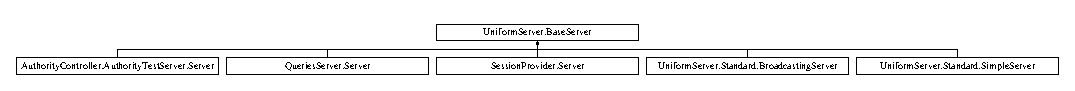
\includegraphics[height=1.021898cm]{d7/d32/class_uniform_server_1_1_base_server}
\end{center}
\end{figure}
\subsection*{Static Public Member Functions}
\begin{DoxyCompactItemize}
\item 
static bool \mbox{\hyperlink{class_uniform_server_1_1_base_server_aefbb2a4287a7f995582b2abf41da8a89}{Send\+Answer\+Via\+PP}} (string answer, \mbox{\hyperlink{struct_uniform_queries_1_1_query_part}{Uniform\+Queries.\+Query\+Part}}\mbox{[}$\,$\mbox{]} entry\+Query\+Parts)
\begin{DoxyCompactList}\small\item\em Open server line using \mbox{\hyperlink{namespace_pipes_provider}{Pipes\+Provider}} that will send answer backward to cliend by dirrect line. Line will established relative to the data shared by client query. \end{DoxyCompactList}\item 
static void \mbox{\hyperlink{class_uniform_server_1_1_base_server_a9ca20516e2a562ddbf8d2c1866f90b25}{Start\+Broadcasting\+Via\+PP}} (string \mbox{\hyperlink{class_uniform_server_1_1_base_server_aaa318b3ed503dd8ccf381c9f3a81ecf2}{pipe\+Name}}, \mbox{\hyperlink{namespace_pipes_provider_1_1_security_a1a6020eca1c661a6f7140e8260502d7e}{Pipes\+Provider.\+Security.\+Security\+Level}} \mbox{\hyperlink{class_uniform_server_1_1_base_server_ac6297faa957fd1005fc61054bdd1cdb1}{security\+Level}}, Broadcasting\+Server\+Transmission\+Controller.\+Message\+Handeler get\+Broadcasting\+Message\+Handler, int chanels)
\begin{DoxyCompactList}\small\item\em Open server with broadcasting chanels using \mbox{\hyperlink{namespace_pipes_provider}{Pipes\+Provider}}. \end{DoxyCompactList}\end{DoxyCompactItemize}
\subsection*{Public Attributes}
\begin{DoxyCompactItemize}
\item 
Thread \mbox{\hyperlink{class_uniform_server_1_1_base_server_a52485a2d70e615a5cbf720c952a8d62f}{thread}}
\begin{DoxyCompactList}\small\item\em Reference to thread that host this server. \end{DoxyCompactList}\item 
string \mbox{\hyperlink{class_uniform_server_1_1_base_server_aaa318b3ed503dd8ccf381c9f3a81ecf2}{pipe\+Name}}
\begin{DoxyCompactList}\small\item\em Name that will be applied to the pipe. \end{DoxyCompactList}\item 
\mbox{\hyperlink{namespace_pipes_provider_1_1_security_a1a6020eca1c661a6f7140e8260502d7e}{Pipes\+Provider.\+Security.\+Security\+Level}} \mbox{\hyperlink{class_uniform_server_1_1_base_server_ac6297faa957fd1005fc61054bdd1cdb1}{security\+Level}} = Pipes\+Provider.\+Security.\+Security\+Level.\+Anonymous
\begin{DoxyCompactList}\small\item\em Squrity level that will applied to pipe. \end{DoxyCompactList}\end{DoxyCompactItemize}
\subsection*{Static Public Attributes}
\begin{DoxyCompactItemize}
\item 
static bool \mbox{\hyperlink{class_uniform_server_1_1_base_server_a632ed557976f4d7bd9b41502bb9a262b}{app\+Terminated}}
\begin{DoxyCompactList}\small\item\em If true then will stop main loop. \end{DoxyCompactList}\end{DoxyCompactItemize}
\subsection*{Protected Member Functions}
\begin{DoxyCompactItemize}
\item 
Thread \mbox{\hyperlink{class_uniform_server_1_1_base_server_aa4a1412b217944e7f8d6ccae6ac68289}{Start\+Server\+Thread}} (string thread\+Name, object shareble\+Param, Parameterized\+Thread\+Start server\+Loop)
\begin{DoxyCompactList}\small\item\em Method that starting server thread. \end{DoxyCompactList}\end{DoxyCompactItemize}
\subsection*{Static Protected Member Functions}
\begin{DoxyCompactItemize}
\item 
static void \mbox{\hyperlink{class_uniform_server_1_1_base_server_a22b92ad517cd1003fe4fe3c86d857169}{Load\+Assemblies}} (string path)
\begin{DoxyCompactList}\small\item\em Loading assemblies from requested path. \end{DoxyCompactList}\item 
static void \mbox{\hyperlink{class_uniform_server_1_1_base_server_a992660752da60019c348e18226a87bf2}{Args\+Reactor}} (string\mbox{[}$\,$\mbox{]} args)
\begin{DoxyCompactList}\small\item\em Method that will configurate application and server relative to the uniform arguments. \end{DoxyCompactList}\item 
static void \mbox{\hyperlink{class_uniform_server_1_1_base_server_a8e9e872bad891b2bc06a8caa6c09ebf9}{Threading\+Server\+Loop\+\_\+\+P\+P\+\_\+\+Output}} (object server)
\begin{DoxyCompactList}\small\item\em Main loop that control monitor thread. \end{DoxyCompactList}\item 
static void \mbox{\hyperlink{class_uniform_server_1_1_base_server_a6cf6b8472de3925d465737a7fc9a8842}{Threading\+Server\+Loop\+\_\+\+P\+P\+\_\+\+Input}} (object server)
\begin{DoxyCompactList}\small\item\em Main loop that control pipe chanel that will recive clients. \end{DoxyCompactList}\item 
static void \mbox{\hyperlink{class_uniform_server_1_1_base_server_ae3c371a7e7953333bb2aa5104fa8a72d}{Threading\+Server\+Loop\+\_\+\+P\+P\+\_\+\+Broadcast}} (object server)
\begin{DoxyCompactList}\small\item\em Main threaded loop that control broadcassting server loop start. \end{DoxyCompactList}\end{DoxyCompactItemize}
\subsection*{Protected Attributes}
\begin{DoxyCompactItemize}
\item 
const int \mbox{\hyperlink{class_uniform_server_1_1_base_server_aaff91507b262d2a1b9021caa2d01640f}{S\+W\+\_\+\+H\+I\+DE}} = 0
\begin{DoxyCompactList}\small\item\em Argument that will hide console window. \end{DoxyCompactList}\item 
const int \mbox{\hyperlink{class_uniform_server_1_1_base_server_a494087cabc03c54c3dc0ac1cc1048860}{S\+W\+\_\+\+S\+H\+OW}} = 5
\begin{DoxyCompactList}\small\item\em Agrument that will show console window. \end{DoxyCompactList}\end{DoxyCompactItemize}
\subsection*{Static Protected Attributes}
\begin{DoxyCompactItemize}
\item 
static int \mbox{\hyperlink{class_uniform_server_1_1_base_server_a4dbe04636a763decfae22ddb2fe26c7a}{thread\+Sleep\+Time}} = 15
\begin{DoxyCompactList}\small\item\em How many milisseconds will sleep thread after tick. \end{DoxyCompactList}\item 
static int \mbox{\hyperlink{class_uniform_server_1_1_base_server_aa40c02a1eec7eda4c36a8ac08119b414}{threads\+Count}} = 1
\begin{DoxyCompactList}\small\item\em Count of threads. \end{DoxyCompactList}\item 
static \mbox{\hyperlink{class_uniform_server_1_1_base_server}{Base\+Server}} \mbox{[}$\,$\mbox{]} \mbox{\hyperlink{class_uniform_server_1_1_base_server_a9c14e919da0c2b9b7f8e57a92c9b0742}{long\+Term\+Server\+Threads}}
\begin{DoxyCompactList}\small\item\em Threads that contai servers. \end{DoxyCompactList}\item 
static Mutex \mbox{\hyperlink{class_uniform_server_1_1_base_server_a051bdce3aec037df76d8efe3b9938198}{mutex\+Obj}} = new Mutex()
\begin{DoxyCompactList}\small\item\em Object that allow to detect processes conflict. \end{DoxyCompactList}\end{DoxyCompactItemize}
\subsection*{Properties}
\begin{DoxyCompactItemize}
\item 
static int \mbox{\hyperlink{class_uniform_server_1_1_base_server_a31cc7d436bb2dd344ec275fd0fa0061e}{Threads\+Count}}\hspace{0.3cm}{\ttfamily  \mbox{[}get, set\mbox{]}}
\begin{DoxyCompactList}\small\item\em Count of threads that will started on server. Changing during fly permited and safely. \end{DoxyCompactList}\end{DoxyCompactItemize}
\subsection*{Events}
\begin{DoxyCompactItemize}
\item 
static System.\+Action$<$ int $>$ \mbox{\hyperlink{class_uniform_server_1_1_base_server_a889c3aaa1cca7f4a9a4e32617516f4be}{Thread\+Terminate\+Request}}
\begin{DoxyCompactList}\small\item\em Event will be called when system will request a thread termination. Argument -\/ index of thread. \end{DoxyCompactList}\item 
static System.\+Action$<$ int $>$ \mbox{\hyperlink{class_uniform_server_1_1_base_server_a440a854a955ab7c5e563918c12e9b32c}{Thread\+Start\+Request}}
\begin{DoxyCompactList}\small\item\em Event that will be called when seystem will require a thread start. Argument -\/ index of thread. \end{DoxyCompactList}\end{DoxyCompactItemize}


\subsection{Detailed Description}
Class that provide base server features and envirounment static A\+PI. 

Part of class that provide methods for establishing transmisssion via \mbox{\hyperlink{namespace_pipes_provider}{Pipes\+Provider}}. 

Part of class that provide methods can be started as thread for server init; 

\subsection{Member Function Documentation}
\mbox{\Hypertarget{class_uniform_server_1_1_base_server_a992660752da60019c348e18226a87bf2}\label{class_uniform_server_1_1_base_server_a992660752da60019c348e18226a87bf2}} 
\index{Uniform\+Server\+::\+Base\+Server@{Uniform\+Server\+::\+Base\+Server}!Args\+Reactor@{Args\+Reactor}}
\index{Args\+Reactor@{Args\+Reactor}!Uniform\+Server\+::\+Base\+Server@{Uniform\+Server\+::\+Base\+Server}}
\subsubsection{\texorpdfstring{Args\+Reactor()}{ArgsReactor()}}
{\footnotesize\ttfamily static void Uniform\+Server.\+Base\+Server.\+Args\+Reactor (\begin{DoxyParamCaption}\item[{string \mbox{[}$\,$\mbox{]}}]{args }\end{DoxyParamCaption})\hspace{0.3cm}{\ttfamily [static]}, {\ttfamily [protected]}}



Method that will configurate application and server relative to the uniform arguments. 


\begin{DoxyParams}{Parameters}
{\em args} & \\
\hline
\end{DoxyParams}
\mbox{\Hypertarget{class_uniform_server_1_1_base_server_a22b92ad517cd1003fe4fe3c86d857169}\label{class_uniform_server_1_1_base_server_a22b92ad517cd1003fe4fe3c86d857169}} 
\index{Uniform\+Server\+::\+Base\+Server@{Uniform\+Server\+::\+Base\+Server}!Load\+Assemblies@{Load\+Assemblies}}
\index{Load\+Assemblies@{Load\+Assemblies}!Uniform\+Server\+::\+Base\+Server@{Uniform\+Server\+::\+Base\+Server}}
\subsubsection{\texorpdfstring{Load\+Assemblies()}{LoadAssemblies()}}
{\footnotesize\ttfamily static void Uniform\+Server.\+Base\+Server.\+Load\+Assemblies (\begin{DoxyParamCaption}\item[{string}]{path }\end{DoxyParamCaption})\hspace{0.3cm}{\ttfamily [static]}, {\ttfamily [protected]}}



Loading assemblies from requested path. 


\begin{DoxyParams}{Parameters}
{\em path} & \\
\hline
\end{DoxyParams}
\mbox{\Hypertarget{class_uniform_server_1_1_base_server_aefbb2a4287a7f995582b2abf41da8a89}\label{class_uniform_server_1_1_base_server_aefbb2a4287a7f995582b2abf41da8a89}} 
\index{Uniform\+Server\+::\+Base\+Server@{Uniform\+Server\+::\+Base\+Server}!Send\+Answer\+Via\+PP@{Send\+Answer\+Via\+PP}}
\index{Send\+Answer\+Via\+PP@{Send\+Answer\+Via\+PP}!Uniform\+Server\+::\+Base\+Server@{Uniform\+Server\+::\+Base\+Server}}
\subsubsection{\texorpdfstring{Send\+Answer\+Via\+P\+P()}{SendAnswerViaPP()}}
{\footnotesize\ttfamily static bool Uniform\+Server.\+Base\+Server.\+Send\+Answer\+Via\+PP (\begin{DoxyParamCaption}\item[{string}]{answer,  }\item[{\mbox{\hyperlink{struct_uniform_queries_1_1_query_part}{Uniform\+Queries.\+Query\+Part}} \mbox{[}$\,$\mbox{]}}]{entry\+Query\+Parts }\end{DoxyParamCaption})\hspace{0.3cm}{\ttfamily [static]}}



Open server line using \mbox{\hyperlink{namespace_pipes_provider}{Pipes\+Provider}} that will send answer backward to cliend by dirrect line. Line will established relative to the data shared by client query. 

Using this method you frovide uniform revers connection and not need to create a transmission line by yourself.

Recommended to use this methos by default dor duplex connection between sever and clients. 


\begin{DoxyParams}{Parameters}
{\em server} & Instance of server that will provide multithreading implementation.\\
\hline
{\em answer} & Message that will sent by server to target client.\\
\hline
{\em entry\+Query\+Parts} & Parts of query that was recived from client. Method will detect core part and establish backward connection.\\
\hline
\end{DoxyParams}
\begin{DoxyReturn}{Returns}

\end{DoxyReturn}
\mbox{\Hypertarget{class_uniform_server_1_1_base_server_a9ca20516e2a562ddbf8d2c1866f90b25}\label{class_uniform_server_1_1_base_server_a9ca20516e2a562ddbf8d2c1866f90b25}} 
\index{Uniform\+Server\+::\+Base\+Server@{Uniform\+Server\+::\+Base\+Server}!Start\+Broadcasting\+Via\+PP@{Start\+Broadcasting\+Via\+PP}}
\index{Start\+Broadcasting\+Via\+PP@{Start\+Broadcasting\+Via\+PP}!Uniform\+Server\+::\+Base\+Server@{Uniform\+Server\+::\+Base\+Server}}
\subsubsection{\texorpdfstring{Start\+Broadcasting\+Via\+P\+P()}{StartBroadcastingViaPP()}}
{\footnotesize\ttfamily static void Uniform\+Server.\+Base\+Server.\+Start\+Broadcasting\+Via\+PP (\begin{DoxyParamCaption}\item[{string}]{pipe\+Name,  }\item[{\mbox{\hyperlink{namespace_pipes_provider_1_1_security_a1a6020eca1c661a6f7140e8260502d7e}{Pipes\+Provider.\+Security.\+Security\+Level}}}]{security\+Level,  }\item[{Broadcasting\+Server\+Transmission\+Controller.\+Message\+Handeler}]{get\+Broadcasting\+Message\+Handler,  }\item[{int}]{chanels }\end{DoxyParamCaption})\hspace{0.3cm}{\ttfamily [static]}}



Open server with broadcasting chanels using \mbox{\hyperlink{namespace_pipes_provider}{Pipes\+Provider}}. 


\begin{DoxyParams}{Parameters}
{\em get\+Broadcasting\+Message\+Handler} & delegate that will be called to get message for new client.\\
\hline
{\em chanels} & How many many connections would awaiable to this server. Attention\+: every chanel is a tread.\\
\hline
\end{DoxyParams}
\mbox{\Hypertarget{class_uniform_server_1_1_base_server_aa4a1412b217944e7f8d6ccae6ac68289}\label{class_uniform_server_1_1_base_server_aa4a1412b217944e7f8d6ccae6ac68289}} 
\index{Uniform\+Server\+::\+Base\+Server@{Uniform\+Server\+::\+Base\+Server}!Start\+Server\+Thread@{Start\+Server\+Thread}}
\index{Start\+Server\+Thread@{Start\+Server\+Thread}!Uniform\+Server\+::\+Base\+Server@{Uniform\+Server\+::\+Base\+Server}}
\subsubsection{\texorpdfstring{Start\+Server\+Thread()}{StartServerThread()}}
{\footnotesize\ttfamily Thread Uniform\+Server.\+Base\+Server.\+Start\+Server\+Thread (\begin{DoxyParamCaption}\item[{string}]{thread\+Name,  }\item[{object}]{shareble\+Param,  }\item[{Parameterized\+Thread\+Start}]{server\+Loop }\end{DoxyParamCaption})\hspace{0.3cm}{\ttfamily [protected]}}



Method that starting server thread. 


\begin{DoxyParams}{Parameters}
{\em thread\+Name} & \\
\hline
{\em shareble\+Param} & \\
\hline
\end{DoxyParams}
\begin{DoxyReturn}{Returns}

\end{DoxyReturn}
\mbox{\Hypertarget{class_uniform_server_1_1_base_server_ae3c371a7e7953333bb2aa5104fa8a72d}\label{class_uniform_server_1_1_base_server_ae3c371a7e7953333bb2aa5104fa8a72d}} 
\index{Uniform\+Server\+::\+Base\+Server@{Uniform\+Server\+::\+Base\+Server}!Threading\+Server\+Loop\+\_\+\+P\+P\+\_\+\+Broadcast@{Threading\+Server\+Loop\+\_\+\+P\+P\+\_\+\+Broadcast}}
\index{Threading\+Server\+Loop\+\_\+\+P\+P\+\_\+\+Broadcast@{Threading\+Server\+Loop\+\_\+\+P\+P\+\_\+\+Broadcast}!Uniform\+Server\+::\+Base\+Server@{Uniform\+Server\+::\+Base\+Server}}
\subsubsection{\texorpdfstring{Threading\+Server\+Loop\+\_\+\+P\+P\+\_\+\+Broadcast()}{ThreadingServerLoop\_PP\_Broadcast()}}
{\footnotesize\ttfamily static void Uniform\+Server.\+Base\+Server.\+Threading\+Server\+Loop\+\_\+\+P\+P\+\_\+\+Broadcast (\begin{DoxyParamCaption}\item[{object}]{server }\end{DoxyParamCaption})\hspace{0.3cm}{\ttfamily [static]}, {\ttfamily [protected]}}



Main threaded loop that control broadcassting server loop start. 

\mbox{\Hypertarget{class_uniform_server_1_1_base_server_a6cf6b8472de3925d465737a7fc9a8842}\label{class_uniform_server_1_1_base_server_a6cf6b8472de3925d465737a7fc9a8842}} 
\index{Uniform\+Server\+::\+Base\+Server@{Uniform\+Server\+::\+Base\+Server}!Threading\+Server\+Loop\+\_\+\+P\+P\+\_\+\+Input@{Threading\+Server\+Loop\+\_\+\+P\+P\+\_\+\+Input}}
\index{Threading\+Server\+Loop\+\_\+\+P\+P\+\_\+\+Input@{Threading\+Server\+Loop\+\_\+\+P\+P\+\_\+\+Input}!Uniform\+Server\+::\+Base\+Server@{Uniform\+Server\+::\+Base\+Server}}
\subsubsection{\texorpdfstring{Threading\+Server\+Loop\+\_\+\+P\+P\+\_\+\+Input()}{ThreadingServerLoop\_PP\_Input()}}
{\footnotesize\ttfamily static void Uniform\+Server.\+Base\+Server.\+Threading\+Server\+Loop\+\_\+\+P\+P\+\_\+\+Input (\begin{DoxyParamCaption}\item[{object}]{server }\end{DoxyParamCaption})\hspace{0.3cm}{\ttfamily [static]}, {\ttfamily [protected]}}



Main loop that control pipe chanel that will recive clients. 

\mbox{\Hypertarget{class_uniform_server_1_1_base_server_a8e9e872bad891b2bc06a8caa6c09ebf9}\label{class_uniform_server_1_1_base_server_a8e9e872bad891b2bc06a8caa6c09ebf9}} 
\index{Uniform\+Server\+::\+Base\+Server@{Uniform\+Server\+::\+Base\+Server}!Threading\+Server\+Loop\+\_\+\+P\+P\+\_\+\+Output@{Threading\+Server\+Loop\+\_\+\+P\+P\+\_\+\+Output}}
\index{Threading\+Server\+Loop\+\_\+\+P\+P\+\_\+\+Output@{Threading\+Server\+Loop\+\_\+\+P\+P\+\_\+\+Output}!Uniform\+Server\+::\+Base\+Server@{Uniform\+Server\+::\+Base\+Server}}
\subsubsection{\texorpdfstring{Threading\+Server\+Loop\+\_\+\+P\+P\+\_\+\+Output()}{ThreadingServerLoop\_PP\_Output()}}
{\footnotesize\ttfamily static void Uniform\+Server.\+Base\+Server.\+Threading\+Server\+Loop\+\_\+\+P\+P\+\_\+\+Output (\begin{DoxyParamCaption}\item[{object}]{server }\end{DoxyParamCaption})\hspace{0.3cm}{\ttfamily [static]}, {\ttfamily [protected]}}



Main loop that control monitor thread. 



\subsection{Member Data Documentation}
\mbox{\Hypertarget{class_uniform_server_1_1_base_server_a632ed557976f4d7bd9b41502bb9a262b}\label{class_uniform_server_1_1_base_server_a632ed557976f4d7bd9b41502bb9a262b}} 
\index{Uniform\+Server\+::\+Base\+Server@{Uniform\+Server\+::\+Base\+Server}!app\+Terminated@{app\+Terminated}}
\index{app\+Terminated@{app\+Terminated}!Uniform\+Server\+::\+Base\+Server@{Uniform\+Server\+::\+Base\+Server}}
\subsubsection{\texorpdfstring{app\+Terminated}{appTerminated}}
{\footnotesize\ttfamily bool Uniform\+Server.\+Base\+Server.\+app\+Terminated\hspace{0.3cm}{\ttfamily [static]}}



If true then will stop main loop. 

\mbox{\Hypertarget{class_uniform_server_1_1_base_server_a9c14e919da0c2b9b7f8e57a92c9b0742}\label{class_uniform_server_1_1_base_server_a9c14e919da0c2b9b7f8e57a92c9b0742}} 
\index{Uniform\+Server\+::\+Base\+Server@{Uniform\+Server\+::\+Base\+Server}!long\+Term\+Server\+Threads@{long\+Term\+Server\+Threads}}
\index{long\+Term\+Server\+Threads@{long\+Term\+Server\+Threads}!Uniform\+Server\+::\+Base\+Server@{Uniform\+Server\+::\+Base\+Server}}
\subsubsection{\texorpdfstring{long\+Term\+Server\+Threads}{longTermServerThreads}}
{\footnotesize\ttfamily \mbox{\hyperlink{class_uniform_server_1_1_base_server}{Base\+Server}} \mbox{[}$\,$\mbox{]} Uniform\+Server.\+Base\+Server.\+long\+Term\+Server\+Threads\hspace{0.3cm}{\ttfamily [static]}, {\ttfamily [protected]}}



Threads that contai servers. 

\mbox{\Hypertarget{class_uniform_server_1_1_base_server_a051bdce3aec037df76d8efe3b9938198}\label{class_uniform_server_1_1_base_server_a051bdce3aec037df76d8efe3b9938198}} 
\index{Uniform\+Server\+::\+Base\+Server@{Uniform\+Server\+::\+Base\+Server}!mutex\+Obj@{mutex\+Obj}}
\index{mutex\+Obj@{mutex\+Obj}!Uniform\+Server\+::\+Base\+Server@{Uniform\+Server\+::\+Base\+Server}}
\subsubsection{\texorpdfstring{mutex\+Obj}{mutexObj}}
{\footnotesize\ttfamily Mutex Uniform\+Server.\+Base\+Server.\+mutex\+Obj = new Mutex()\hspace{0.3cm}{\ttfamily [static]}, {\ttfamily [protected]}}



Object that allow to detect processes conflict. 

\mbox{\Hypertarget{class_uniform_server_1_1_base_server_aaa318b3ed503dd8ccf381c9f3a81ecf2}\label{class_uniform_server_1_1_base_server_aaa318b3ed503dd8ccf381c9f3a81ecf2}} 
\index{Uniform\+Server\+::\+Base\+Server@{Uniform\+Server\+::\+Base\+Server}!pipe\+Name@{pipe\+Name}}
\index{pipe\+Name@{pipe\+Name}!Uniform\+Server\+::\+Base\+Server@{Uniform\+Server\+::\+Base\+Server}}
\subsubsection{\texorpdfstring{pipe\+Name}{pipeName}}
{\footnotesize\ttfamily string Uniform\+Server.\+Base\+Server.\+pipe\+Name}



Name that will be applied to the pipe. 

\mbox{\Hypertarget{class_uniform_server_1_1_base_server_ac6297faa957fd1005fc61054bdd1cdb1}\label{class_uniform_server_1_1_base_server_ac6297faa957fd1005fc61054bdd1cdb1}} 
\index{Uniform\+Server\+::\+Base\+Server@{Uniform\+Server\+::\+Base\+Server}!security\+Level@{security\+Level}}
\index{security\+Level@{security\+Level}!Uniform\+Server\+::\+Base\+Server@{Uniform\+Server\+::\+Base\+Server}}
\subsubsection{\texorpdfstring{security\+Level}{securityLevel}}
{\footnotesize\ttfamily \mbox{\hyperlink{namespace_pipes_provider_1_1_security_a1a6020eca1c661a6f7140e8260502d7e}{Pipes\+Provider.\+Security.\+Security\+Level}} Uniform\+Server.\+Base\+Server.\+security\+Level = Pipes\+Provider.\+Security.\+Security\+Level.\+Anonymous}



Squrity level that will applied to pipe. 

\mbox{\Hypertarget{class_uniform_server_1_1_base_server_aaff91507b262d2a1b9021caa2d01640f}\label{class_uniform_server_1_1_base_server_aaff91507b262d2a1b9021caa2d01640f}} 
\index{Uniform\+Server\+::\+Base\+Server@{Uniform\+Server\+::\+Base\+Server}!S\+W\+\_\+\+H\+I\+DE@{S\+W\+\_\+\+H\+I\+DE}}
\index{S\+W\+\_\+\+H\+I\+DE@{S\+W\+\_\+\+H\+I\+DE}!Uniform\+Server\+::\+Base\+Server@{Uniform\+Server\+::\+Base\+Server}}
\subsubsection{\texorpdfstring{S\+W\+\_\+\+H\+I\+DE}{SW\_HIDE}}
{\footnotesize\ttfamily const int Uniform\+Server.\+Base\+Server.\+S\+W\+\_\+\+H\+I\+DE = 0\hspace{0.3cm}{\ttfamily [protected]}}



Argument that will hide console window. 

\mbox{\Hypertarget{class_uniform_server_1_1_base_server_a494087cabc03c54c3dc0ac1cc1048860}\label{class_uniform_server_1_1_base_server_a494087cabc03c54c3dc0ac1cc1048860}} 
\index{Uniform\+Server\+::\+Base\+Server@{Uniform\+Server\+::\+Base\+Server}!S\+W\+\_\+\+S\+H\+OW@{S\+W\+\_\+\+S\+H\+OW}}
\index{S\+W\+\_\+\+S\+H\+OW@{S\+W\+\_\+\+S\+H\+OW}!Uniform\+Server\+::\+Base\+Server@{Uniform\+Server\+::\+Base\+Server}}
\subsubsection{\texorpdfstring{S\+W\+\_\+\+S\+H\+OW}{SW\_SHOW}}
{\footnotesize\ttfamily const int Uniform\+Server.\+Base\+Server.\+S\+W\+\_\+\+S\+H\+OW = 5\hspace{0.3cm}{\ttfamily [protected]}}



Agrument that will show console window. 

\mbox{\Hypertarget{class_uniform_server_1_1_base_server_a52485a2d70e615a5cbf720c952a8d62f}\label{class_uniform_server_1_1_base_server_a52485a2d70e615a5cbf720c952a8d62f}} 
\index{Uniform\+Server\+::\+Base\+Server@{Uniform\+Server\+::\+Base\+Server}!thread@{thread}}
\index{thread@{thread}!Uniform\+Server\+::\+Base\+Server@{Uniform\+Server\+::\+Base\+Server}}
\subsubsection{\texorpdfstring{thread}{thread}}
{\footnotesize\ttfamily Thread Uniform\+Server.\+Base\+Server.\+thread}



Reference to thread that host this server. 

\mbox{\Hypertarget{class_uniform_server_1_1_base_server_aa40c02a1eec7eda4c36a8ac08119b414}\label{class_uniform_server_1_1_base_server_aa40c02a1eec7eda4c36a8ac08119b414}} 
\index{Uniform\+Server\+::\+Base\+Server@{Uniform\+Server\+::\+Base\+Server}!threads\+Count@{threads\+Count}}
\index{threads\+Count@{threads\+Count}!Uniform\+Server\+::\+Base\+Server@{Uniform\+Server\+::\+Base\+Server}}
\subsubsection{\texorpdfstring{threads\+Count}{threadsCount}}
{\footnotesize\ttfamily int Uniform\+Server.\+Base\+Server.\+threads\+Count = 1\hspace{0.3cm}{\ttfamily [static]}, {\ttfamily [protected]}}



Count of threads. 

\mbox{\Hypertarget{class_uniform_server_1_1_base_server_a4dbe04636a763decfae22ddb2fe26c7a}\label{class_uniform_server_1_1_base_server_a4dbe04636a763decfae22ddb2fe26c7a}} 
\index{Uniform\+Server\+::\+Base\+Server@{Uniform\+Server\+::\+Base\+Server}!thread\+Sleep\+Time@{thread\+Sleep\+Time}}
\index{thread\+Sleep\+Time@{thread\+Sleep\+Time}!Uniform\+Server\+::\+Base\+Server@{Uniform\+Server\+::\+Base\+Server}}
\subsubsection{\texorpdfstring{thread\+Sleep\+Time}{threadSleepTime}}
{\footnotesize\ttfamily int Uniform\+Server.\+Base\+Server.\+thread\+Sleep\+Time = 15\hspace{0.3cm}{\ttfamily [static]}, {\ttfamily [protected]}}



How many milisseconds will sleep thread after tick. 



\subsection{Property Documentation}
\mbox{\Hypertarget{class_uniform_server_1_1_base_server_a31cc7d436bb2dd344ec275fd0fa0061e}\label{class_uniform_server_1_1_base_server_a31cc7d436bb2dd344ec275fd0fa0061e}} 
\index{Uniform\+Server\+::\+Base\+Server@{Uniform\+Server\+::\+Base\+Server}!Threads\+Count@{Threads\+Count}}
\index{Threads\+Count@{Threads\+Count}!Uniform\+Server\+::\+Base\+Server@{Uniform\+Server\+::\+Base\+Server}}
\subsubsection{\texorpdfstring{Threads\+Count}{ThreadsCount}}
{\footnotesize\ttfamily int Uniform\+Server.\+Base\+Server.\+Threads\+Count\hspace{0.3cm}{\ttfamily [static]}, {\ttfamily [get]}, {\ttfamily [set]}}



Count of threads that will started on server. Changing during fly permited and safely. 



\subsection{Event Documentation}
\mbox{\Hypertarget{class_uniform_server_1_1_base_server_a440a854a955ab7c5e563918c12e9b32c}\label{class_uniform_server_1_1_base_server_a440a854a955ab7c5e563918c12e9b32c}} 
\index{Uniform\+Server\+::\+Base\+Server@{Uniform\+Server\+::\+Base\+Server}!Thread\+Start\+Request@{Thread\+Start\+Request}}
\index{Thread\+Start\+Request@{Thread\+Start\+Request}!Uniform\+Server\+::\+Base\+Server@{Uniform\+Server\+::\+Base\+Server}}
\subsubsection{\texorpdfstring{Thread\+Start\+Request}{ThreadStartRequest}}
{\footnotesize\ttfamily System.\+Action$<$int$>$ Uniform\+Server.\+Base\+Server.\+Thread\+Start\+Request\hspace{0.3cm}{\ttfamily [static]}}



Event that will be called when seystem will require a thread start. Argument -\/ index of thread. 

\mbox{\Hypertarget{class_uniform_server_1_1_base_server_a889c3aaa1cca7f4a9a4e32617516f4be}\label{class_uniform_server_1_1_base_server_a889c3aaa1cca7f4a9a4e32617516f4be}} 
\index{Uniform\+Server\+::\+Base\+Server@{Uniform\+Server\+::\+Base\+Server}!Thread\+Terminate\+Request@{Thread\+Terminate\+Request}}
\index{Thread\+Terminate\+Request@{Thread\+Terminate\+Request}!Uniform\+Server\+::\+Base\+Server@{Uniform\+Server\+::\+Base\+Server}}
\subsubsection{\texorpdfstring{Thread\+Terminate\+Request}{ThreadTerminateRequest}}
{\footnotesize\ttfamily System.\+Action$<$int$>$ Uniform\+Server.\+Base\+Server.\+Thread\+Terminate\+Request\hspace{0.3cm}{\ttfamily [static]}}



Event will be called when system will request a thread termination. Argument -\/ index of thread. 



The documentation for this class was generated from the following files\+:\begin{DoxyCompactItemize}
\item 
D\+:/\+Work/\+Git\+Hub/doloro-\/networking-\/framework/\+Core/\+Uniform\+Server/\+Providers/Base\+Server.\+cs\item 
D\+:/\+Work/\+Git\+Hub/doloro-\/networking-\/framework/\+Core/\+Uniform\+Server/\+Providers/\+Pipes\+Provider/Base\+Server\+P\+P\+Threading.\+cs\item 
D\+:/\+Work/\+Git\+Hub/doloro-\/networking-\/framework/\+Core/\+Uniform\+Server/\+Providers/\+Pipes\+Provider/Base\+Server\+P\+P\+Transmission.\+cs\end{DoxyCompactItemize}

\hypertarget{class_pipes_provider_1_1_server_1_1_transmission_controllers_1_1_base_server_transmission_controller}{}\section{Pipes\+Provider.\+Server.\+Transmission\+Controllers.\+Base\+Server\+Transmission\+Controller Class Reference}
\label{class_pipes_provider_1_1_server_1_1_transmission_controllers_1_1_base_server_transmission_controller}\index{Pipes\+Provider.\+Server.\+Transmission\+Controllers.\+Base\+Server\+Transmission\+Controller@{Pipes\+Provider.\+Server.\+Transmission\+Controllers.\+Base\+Server\+Transmission\+Controller}}


Container that contain meta data about server instance.  


Inheritance diagram for Pipes\+Provider.\+Server.\+Transmission\+Controllers.\+Base\+Server\+Transmission\+Controller\+:\begin{figure}[H]
\begin{center}
\leavevmode
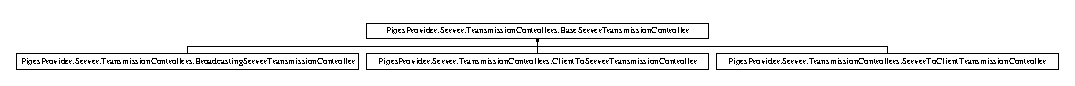
\includegraphics[height=0.707071cm]{d0/d5b/class_pipes_provider_1_1_server_1_1_transmission_controllers_1_1_base_server_transmission_controller}
\end{center}
\end{figure}
\subsection*{Public Member Functions}
\begin{DoxyCompactItemize}
\item 
\mbox{\Hypertarget{class_pipes_provider_1_1_server_1_1_transmission_controllers_1_1_base_server_transmission_controller_ad3ffb9dd45062b59d88dd08f9df90c5f}\label{class_pipes_provider_1_1_server_1_1_transmission_controllers_1_1_base_server_transmission_controller_ad3ffb9dd45062b59d88dd08f9df90c5f}} 
{\bfseries Base\+Server\+Transmission\+Controller} (I\+Async\+Result \mbox{\hyperlink{class_pipes_provider_1_1_server_1_1_transmission_controllers_1_1_base_server_transmission_controller_afc45a2287e6fef24892a0aee8aa86f56}{connection\+Marker}}, System.\+Action$<$ \mbox{\hyperlink{class_pipes_provider_1_1_server_1_1_transmission_controllers_1_1_base_server_transmission_controller}{Base\+Server\+Transmission\+Controller}} $>$ \mbox{\hyperlink{class_pipes_provider_1_1_server_1_1_transmission_controllers_1_1_base_server_transmission_controller_a632261255d8dfc87d93445180c6e2c9d}{connection\+Callback}}, Named\+Pipe\+Server\+Stream pipe, string \mbox{\hyperlink{class_pipes_provider_1_1_server_1_1_transmission_controllers_1_1_base_server_transmission_controller_a4ce9911f1ad6814d3e5c9096d9ddde57}{pipe\+Name}})
\item 
void \mbox{\hyperlink{class_pipes_provider_1_1_server_1_1_transmission_controllers_1_1_base_server_transmission_controller_a6123ecf83e5ed7d39e8fe457681e3bfc}{Set\+Expired}} ()
\begin{DoxyCompactList}\small\item\em Maeking transmission as expired. Line will be remaked. \end{DoxyCompactList}\item 
void \mbox{\hyperlink{class_pipes_provider_1_1_server_1_1_transmission_controllers_1_1_base_server_transmission_controller_a838c1d62567059bbe92e9be3eca971d5}{Set\+Stoped}} ()
\begin{DoxyCompactList}\small\item\em Marking transmission as expired and stoped for full exclusion from automatic server operations. \end{DoxyCompactList}\end{DoxyCompactItemize}
\subsection*{Public Attributes}
\begin{DoxyCompactItemize}
\item 
I\+Async\+Result \mbox{\hyperlink{class_pipes_provider_1_1_server_1_1_transmission_controllers_1_1_base_server_transmission_controller_afc45a2287e6fef24892a0aee8aa86f56}{connection\+Marker}}
\begin{DoxyCompactList}\small\item\em Object that provide access to async connection. \end{DoxyCompactList}\item 
System.\+Action$<$ \mbox{\hyperlink{class_pipes_provider_1_1_server_1_1_transmission_controllers_1_1_base_server_transmission_controller}{Base\+Server\+Transmission\+Controller}} $>$ \mbox{\hyperlink{class_pipes_provider_1_1_server_1_1_transmission_controllers_1_1_base_server_transmission_controller_a632261255d8dfc87d93445180c6e2c9d}{connection\+Callback}}
\begin{DoxyCompactList}\small\item\em Delegate that will be called when connection will be established. Server\+Transmission\+Meta -\/ meta data of transmission. \end{DoxyCompactList}\item 
Named\+Pipe\+Server\+Stream \mbox{\hyperlink{class_pipes_provider_1_1_server_1_1_transmission_controllers_1_1_base_server_transmission_controller_a019f764411256a751f8a438076426a47}{pipe\+Server}}
\begin{DoxyCompactList}\small\item\em Reference to created pipe. \end{DoxyCompactList}\item 
string \mbox{\hyperlink{class_pipes_provider_1_1_server_1_1_transmission_controllers_1_1_base_server_transmission_controller_a4ce9911f1ad6814d3e5c9096d9ddde57}{pipe\+Name}}
\begin{DoxyCompactList}\small\item\em Name of this connection. \end{DoxyCompactList}\end{DoxyCompactItemize}
\subsection*{Properties}
\begin{DoxyCompactItemize}
\item 
bool \mbox{\hyperlink{class_pipes_provider_1_1_server_1_1_transmission_controllers_1_1_base_server_transmission_controller_ad57a0420e71e3897e7e1b67c16b995f6}{Expired}}\hspace{0.3cm}{\ttfamily  \mbox{[}get, protected set\mbox{]}}
\begin{DoxyCompactList}\small\item\em Marker that show does current transmission is relevant. When it\textquotesingle{}ll become true this pipe connection will be desconected. \end{DoxyCompactList}\item 
bool \mbox{\hyperlink{class_pipes_provider_1_1_server_1_1_transmission_controllers_1_1_base_server_transmission_controller_ae159fdf4582f9419d9e3616d2aa2d37e}{Stoped}}\hspace{0.3cm}{\ttfamily  \mbox{[}get, protected set\mbox{]}}
\begin{DoxyCompactList}\small\item\em Marker that show does this transmition stoped. \end{DoxyCompactList}\item 
static \mbox{\hyperlink{class_pipes_provider_1_1_server_1_1_transmission_controllers_1_1_base_server_transmission_controller}{Base\+Server\+Transmission\+Controller}} \mbox{\hyperlink{class_pipes_provider_1_1_server_1_1_transmission_controllers_1_1_base_server_transmission_controller_af60aaebfbfe6988e008cedb18f32c759}{None}}\hspace{0.3cm}{\ttfamily  \mbox{[}get\mbox{]}}
\begin{DoxyCompactList}\small\item\em Return instance that not contain initialized fields. \end{DoxyCompactList}\end{DoxyCompactItemize}


\subsection{Detailed Description}
Container that contain meta data about server instance. 



\subsection{Member Function Documentation}
\mbox{\Hypertarget{class_pipes_provider_1_1_server_1_1_transmission_controllers_1_1_base_server_transmission_controller_a6123ecf83e5ed7d39e8fe457681e3bfc}\label{class_pipes_provider_1_1_server_1_1_transmission_controllers_1_1_base_server_transmission_controller_a6123ecf83e5ed7d39e8fe457681e3bfc}} 
\index{Pipes\+Provider\+::\+Server\+::\+Transmission\+Controllers\+::\+Base\+Server\+Transmission\+Controller@{Pipes\+Provider\+::\+Server\+::\+Transmission\+Controllers\+::\+Base\+Server\+Transmission\+Controller}!Set\+Expired@{Set\+Expired}}
\index{Set\+Expired@{Set\+Expired}!Pipes\+Provider\+::\+Server\+::\+Transmission\+Controllers\+::\+Base\+Server\+Transmission\+Controller@{Pipes\+Provider\+::\+Server\+::\+Transmission\+Controllers\+::\+Base\+Server\+Transmission\+Controller}}
\subsubsection{\texorpdfstring{Set\+Expired()}{SetExpired()}}
{\footnotesize\ttfamily void Pipes\+Provider.\+Server.\+Transmission\+Controllers.\+Base\+Server\+Transmission\+Controller.\+Set\+Expired (\begin{DoxyParamCaption}{ }\end{DoxyParamCaption})}



Maeking transmission as expired. Line will be remaked. 

\mbox{\Hypertarget{class_pipes_provider_1_1_server_1_1_transmission_controllers_1_1_base_server_transmission_controller_a838c1d62567059bbe92e9be3eca971d5}\label{class_pipes_provider_1_1_server_1_1_transmission_controllers_1_1_base_server_transmission_controller_a838c1d62567059bbe92e9be3eca971d5}} 
\index{Pipes\+Provider\+::\+Server\+::\+Transmission\+Controllers\+::\+Base\+Server\+Transmission\+Controller@{Pipes\+Provider\+::\+Server\+::\+Transmission\+Controllers\+::\+Base\+Server\+Transmission\+Controller}!Set\+Stoped@{Set\+Stoped}}
\index{Set\+Stoped@{Set\+Stoped}!Pipes\+Provider\+::\+Server\+::\+Transmission\+Controllers\+::\+Base\+Server\+Transmission\+Controller@{Pipes\+Provider\+::\+Server\+::\+Transmission\+Controllers\+::\+Base\+Server\+Transmission\+Controller}}
\subsubsection{\texorpdfstring{Set\+Stoped()}{SetStoped()}}
{\footnotesize\ttfamily void Pipes\+Provider.\+Server.\+Transmission\+Controllers.\+Base\+Server\+Transmission\+Controller.\+Set\+Stoped (\begin{DoxyParamCaption}{ }\end{DoxyParamCaption})}



Marking transmission as expired and stoped for full exclusion from automatic server operations. 



\subsection{Member Data Documentation}
\mbox{\Hypertarget{class_pipes_provider_1_1_server_1_1_transmission_controllers_1_1_base_server_transmission_controller_a632261255d8dfc87d93445180c6e2c9d}\label{class_pipes_provider_1_1_server_1_1_transmission_controllers_1_1_base_server_transmission_controller_a632261255d8dfc87d93445180c6e2c9d}} 
\index{Pipes\+Provider\+::\+Server\+::\+Transmission\+Controllers\+::\+Base\+Server\+Transmission\+Controller@{Pipes\+Provider\+::\+Server\+::\+Transmission\+Controllers\+::\+Base\+Server\+Transmission\+Controller}!connection\+Callback@{connection\+Callback}}
\index{connection\+Callback@{connection\+Callback}!Pipes\+Provider\+::\+Server\+::\+Transmission\+Controllers\+::\+Base\+Server\+Transmission\+Controller@{Pipes\+Provider\+::\+Server\+::\+Transmission\+Controllers\+::\+Base\+Server\+Transmission\+Controller}}
\subsubsection{\texorpdfstring{connection\+Callback}{connectionCallback}}
{\footnotesize\ttfamily System.\+Action$<$\mbox{\hyperlink{class_pipes_provider_1_1_server_1_1_transmission_controllers_1_1_base_server_transmission_controller}{Base\+Server\+Transmission\+Controller}}$>$ Pipes\+Provider.\+Server.\+Transmission\+Controllers.\+Base\+Server\+Transmission\+Controller.\+connection\+Callback}



Delegate that will be called when connection will be established. Server\+Transmission\+Meta -\/ meta data of transmission. 

\mbox{\Hypertarget{class_pipes_provider_1_1_server_1_1_transmission_controllers_1_1_base_server_transmission_controller_afc45a2287e6fef24892a0aee8aa86f56}\label{class_pipes_provider_1_1_server_1_1_transmission_controllers_1_1_base_server_transmission_controller_afc45a2287e6fef24892a0aee8aa86f56}} 
\index{Pipes\+Provider\+::\+Server\+::\+Transmission\+Controllers\+::\+Base\+Server\+Transmission\+Controller@{Pipes\+Provider\+::\+Server\+::\+Transmission\+Controllers\+::\+Base\+Server\+Transmission\+Controller}!connection\+Marker@{connection\+Marker}}
\index{connection\+Marker@{connection\+Marker}!Pipes\+Provider\+::\+Server\+::\+Transmission\+Controllers\+::\+Base\+Server\+Transmission\+Controller@{Pipes\+Provider\+::\+Server\+::\+Transmission\+Controllers\+::\+Base\+Server\+Transmission\+Controller}}
\subsubsection{\texorpdfstring{connection\+Marker}{connectionMarker}}
{\footnotesize\ttfamily I\+Async\+Result Pipes\+Provider.\+Server.\+Transmission\+Controllers.\+Base\+Server\+Transmission\+Controller.\+connection\+Marker}



Object that provide access to async connection. 

\mbox{\Hypertarget{class_pipes_provider_1_1_server_1_1_transmission_controllers_1_1_base_server_transmission_controller_a4ce9911f1ad6814d3e5c9096d9ddde57}\label{class_pipes_provider_1_1_server_1_1_transmission_controllers_1_1_base_server_transmission_controller_a4ce9911f1ad6814d3e5c9096d9ddde57}} 
\index{Pipes\+Provider\+::\+Server\+::\+Transmission\+Controllers\+::\+Base\+Server\+Transmission\+Controller@{Pipes\+Provider\+::\+Server\+::\+Transmission\+Controllers\+::\+Base\+Server\+Transmission\+Controller}!pipe\+Name@{pipe\+Name}}
\index{pipe\+Name@{pipe\+Name}!Pipes\+Provider\+::\+Server\+::\+Transmission\+Controllers\+::\+Base\+Server\+Transmission\+Controller@{Pipes\+Provider\+::\+Server\+::\+Transmission\+Controllers\+::\+Base\+Server\+Transmission\+Controller}}
\subsubsection{\texorpdfstring{pipe\+Name}{pipeName}}
{\footnotesize\ttfamily string Pipes\+Provider.\+Server.\+Transmission\+Controllers.\+Base\+Server\+Transmission\+Controller.\+pipe\+Name}



Name of this connection. 

\mbox{\Hypertarget{class_pipes_provider_1_1_server_1_1_transmission_controllers_1_1_base_server_transmission_controller_a019f764411256a751f8a438076426a47}\label{class_pipes_provider_1_1_server_1_1_transmission_controllers_1_1_base_server_transmission_controller_a019f764411256a751f8a438076426a47}} 
\index{Pipes\+Provider\+::\+Server\+::\+Transmission\+Controllers\+::\+Base\+Server\+Transmission\+Controller@{Pipes\+Provider\+::\+Server\+::\+Transmission\+Controllers\+::\+Base\+Server\+Transmission\+Controller}!pipe\+Server@{pipe\+Server}}
\index{pipe\+Server@{pipe\+Server}!Pipes\+Provider\+::\+Server\+::\+Transmission\+Controllers\+::\+Base\+Server\+Transmission\+Controller@{Pipes\+Provider\+::\+Server\+::\+Transmission\+Controllers\+::\+Base\+Server\+Transmission\+Controller}}
\subsubsection{\texorpdfstring{pipe\+Server}{pipeServer}}
{\footnotesize\ttfamily Named\+Pipe\+Server\+Stream Pipes\+Provider.\+Server.\+Transmission\+Controllers.\+Base\+Server\+Transmission\+Controller.\+pipe\+Server}



Reference to created pipe. 



\subsection{Property Documentation}
\mbox{\Hypertarget{class_pipes_provider_1_1_server_1_1_transmission_controllers_1_1_base_server_transmission_controller_ad57a0420e71e3897e7e1b67c16b995f6}\label{class_pipes_provider_1_1_server_1_1_transmission_controllers_1_1_base_server_transmission_controller_ad57a0420e71e3897e7e1b67c16b995f6}} 
\index{Pipes\+Provider\+::\+Server\+::\+Transmission\+Controllers\+::\+Base\+Server\+Transmission\+Controller@{Pipes\+Provider\+::\+Server\+::\+Transmission\+Controllers\+::\+Base\+Server\+Transmission\+Controller}!Expired@{Expired}}
\index{Expired@{Expired}!Pipes\+Provider\+::\+Server\+::\+Transmission\+Controllers\+::\+Base\+Server\+Transmission\+Controller@{Pipes\+Provider\+::\+Server\+::\+Transmission\+Controllers\+::\+Base\+Server\+Transmission\+Controller}}
\subsubsection{\texorpdfstring{Expired}{Expired}}
{\footnotesize\ttfamily bool Pipes\+Provider.\+Server.\+Transmission\+Controllers.\+Base\+Server\+Transmission\+Controller.\+Expired\hspace{0.3cm}{\ttfamily [get]}, {\ttfamily [protected set]}}



Marker that show does current transmission is relevant. When it\textquotesingle{}ll become true this pipe connection will be desconected. 

\mbox{\Hypertarget{class_pipes_provider_1_1_server_1_1_transmission_controllers_1_1_base_server_transmission_controller_af60aaebfbfe6988e008cedb18f32c759}\label{class_pipes_provider_1_1_server_1_1_transmission_controllers_1_1_base_server_transmission_controller_af60aaebfbfe6988e008cedb18f32c759}} 
\index{Pipes\+Provider\+::\+Server\+::\+Transmission\+Controllers\+::\+Base\+Server\+Transmission\+Controller@{Pipes\+Provider\+::\+Server\+::\+Transmission\+Controllers\+::\+Base\+Server\+Transmission\+Controller}!None@{None}}
\index{None@{None}!Pipes\+Provider\+::\+Server\+::\+Transmission\+Controllers\+::\+Base\+Server\+Transmission\+Controller@{Pipes\+Provider\+::\+Server\+::\+Transmission\+Controllers\+::\+Base\+Server\+Transmission\+Controller}}
\subsubsection{\texorpdfstring{None}{None}}
{\footnotesize\ttfamily \mbox{\hyperlink{class_pipes_provider_1_1_server_1_1_transmission_controllers_1_1_base_server_transmission_controller}{Base\+Server\+Transmission\+Controller}} Pipes\+Provider.\+Server.\+Transmission\+Controllers.\+Base\+Server\+Transmission\+Controller.\+None\hspace{0.3cm}{\ttfamily [static]}, {\ttfamily [get]}}



Return instance that not contain initialized fields. 

\mbox{\Hypertarget{class_pipes_provider_1_1_server_1_1_transmission_controllers_1_1_base_server_transmission_controller_ae159fdf4582f9419d9e3616d2aa2d37e}\label{class_pipes_provider_1_1_server_1_1_transmission_controllers_1_1_base_server_transmission_controller_ae159fdf4582f9419d9e3616d2aa2d37e}} 
\index{Pipes\+Provider\+::\+Server\+::\+Transmission\+Controllers\+::\+Base\+Server\+Transmission\+Controller@{Pipes\+Provider\+::\+Server\+::\+Transmission\+Controllers\+::\+Base\+Server\+Transmission\+Controller}!Stoped@{Stoped}}
\index{Stoped@{Stoped}!Pipes\+Provider\+::\+Server\+::\+Transmission\+Controllers\+::\+Base\+Server\+Transmission\+Controller@{Pipes\+Provider\+::\+Server\+::\+Transmission\+Controllers\+::\+Base\+Server\+Transmission\+Controller}}
\subsubsection{\texorpdfstring{Stoped}{Stoped}}
{\footnotesize\ttfamily bool Pipes\+Provider.\+Server.\+Transmission\+Controllers.\+Base\+Server\+Transmission\+Controller.\+Stoped\hspace{0.3cm}{\ttfamily [get]}, {\ttfamily [protected set]}}



Marker that show does this transmition stoped. 



The documentation for this class was generated from the following file\+:\begin{DoxyCompactItemize}
\item 
D\+:/\+Work/\+Git\+Hub/doloro-\/networking-\/framework/\+Pipes\+Provider/\+Server/\+Transmisssion\+Controllers/Base\+Server\+Transmission\+Controller.\+cs\end{DoxyCompactItemize}

\hypertarget{class_uniform_server_1_1_standard_1_1_broadcasting_server}{}\section{Uniform\+Server.\+Standard.\+Broadcasting\+Server Class Reference}
\label{class_uniform_server_1_1_standard_1_1_broadcasting_server}\index{Uniform\+Server.\+Standard.\+Broadcasting\+Server@{Uniform\+Server.\+Standard.\+Broadcasting\+Server}}


Server that allow instiniate \mbox{\hyperlink{class_uniform_server_1_1_base_server}{Base\+Server}}. Not contain any additive methods.  


Inheritance diagram for Uniform\+Server.\+Standard.\+Broadcasting\+Server\+:\begin{figure}[H]
\begin{center}
\leavevmode
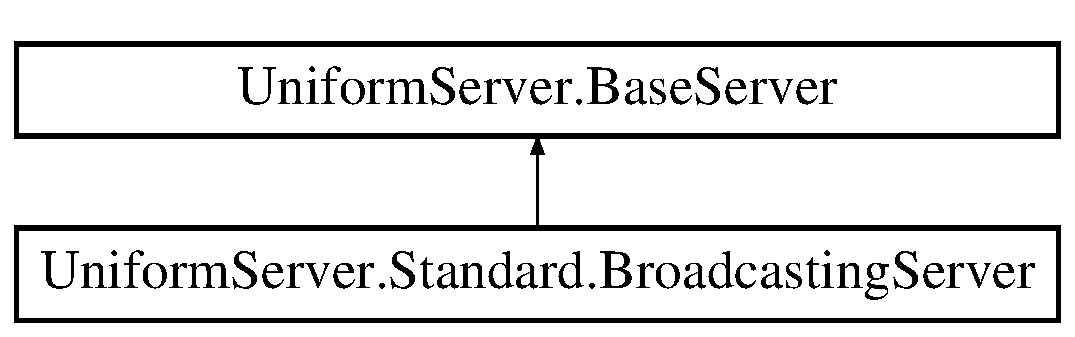
\includegraphics[height=2.000000cm]{d5/dac/class_uniform_server_1_1_standard_1_1_broadcasting_server}
\end{center}
\end{figure}
\subsection*{Public Attributes}
\begin{DoxyCompactItemize}
\item 
\mbox{\Hypertarget{class_uniform_server_1_1_standard_1_1_broadcasting_server_a0c09cadabd5e8c941979bc7b32185c79}\label{class_uniform_server_1_1_standard_1_1_broadcasting_server_a0c09cadabd5e8c941979bc7b32185c79}} 
Broadcasting\+Server\+Transmission\+Controller.\+Message\+Handeler {\bfseries Get\+Message}
\end{DoxyCompactItemize}
\subsection*{Additional Inherited Members}


\subsection{Detailed Description}
Server that allow instiniate \mbox{\hyperlink{class_uniform_server_1_1_base_server}{Base\+Server}}. Not contain any additive methods. 

Case of using -\/ simple operations like registing of server for answer. 

The documentation for this class was generated from the following file\+:\begin{DoxyCompactItemize}
\item 
D\+:/\+Work/\+Git\+Hub/doloro-\/networking-\/framework/\+Uniform\+Server/\+Providers/\+Standard/Broadcasting\+Server.\+cs\end{DoxyCompactItemize}

\hypertarget{class_pipes_provider_1_1_server_1_1_transmission_controllers_1_1_broadcasting_server_transmission_controller}{}\section{Pipes\+Provider.\+Server.\+Transmission\+Controllers.\+Broadcasting\+Server\+Transmission\+Controller Class Reference}
\label{class_pipes_provider_1_1_server_1_1_transmission_controllers_1_1_broadcasting_server_transmission_controller}\index{Pipes\+Provider.\+Server.\+Transmission\+Controllers.\+Broadcasting\+Server\+Transmission\+Controller@{Pipes\+Provider.\+Server.\+Transmission\+Controllers.\+Broadcasting\+Server\+Transmission\+Controller}}


Transmission controller that situable for broadcasting. Every connection will call Message handler that can share scripted or constant data.  


Inheritance diagram for Pipes\+Provider.\+Server.\+Transmission\+Controllers.\+Broadcasting\+Server\+Transmission\+Controller\+:\begin{figure}[H]
\begin{center}
\leavevmode
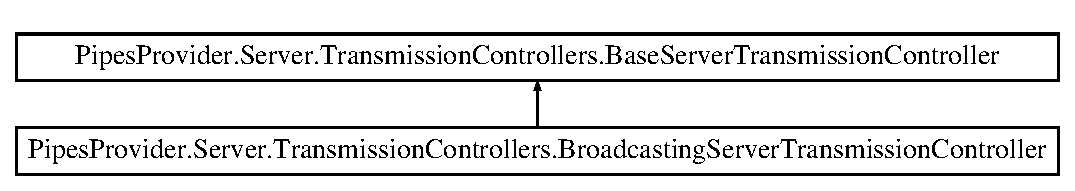
\includegraphics[height=2.000000cm]{db/df3/class_pipes_provider_1_1_server_1_1_transmission_controllers_1_1_broadcasting_server_transmission_controller}
\end{center}
\end{figure}
\subsection*{Public Member Functions}
\begin{DoxyCompactItemize}
\item 
\mbox{\Hypertarget{class_pipes_provider_1_1_server_1_1_transmission_controllers_1_1_broadcasting_server_transmission_controller_ace17cd03bcec52f8e9a7a980ccae25fb}\label{class_pipes_provider_1_1_server_1_1_transmission_controllers_1_1_broadcasting_server_transmission_controller_ace17cd03bcec52f8e9a7a980ccae25fb}} 
delegate string {\bfseries Message\+Handeler} ()
\item 
\mbox{\Hypertarget{class_pipes_provider_1_1_server_1_1_transmission_controllers_1_1_broadcasting_server_transmission_controller_a571cf673b8b112d837bd069dfa83f58b}\label{class_pipes_provider_1_1_server_1_1_transmission_controllers_1_1_broadcasting_server_transmission_controller_a571cf673b8b112d837bd069dfa83f58b}} 
{\bfseries Broadcasting\+Server\+Transmission\+Controller} (I\+Async\+Result \mbox{\hyperlink{class_pipes_provider_1_1_server_1_1_transmission_controllers_1_1_base_server_transmission_controller_afc45a2287e6fef24892a0aee8aa86f56}{connection\+Marker}}, System.\+Action$<$ \mbox{\hyperlink{class_pipes_provider_1_1_server_1_1_transmission_controllers_1_1_base_server_transmission_controller}{Base\+Server\+Transmission\+Controller}} $>$ \mbox{\hyperlink{class_pipes_provider_1_1_server_1_1_transmission_controllers_1_1_base_server_transmission_controller_a632261255d8dfc87d93445180c6e2c9d}{connection\+Callback}}, Named\+Pipe\+Server\+Stream pipe, string \mbox{\hyperlink{class_pipes_provider_1_1_server_1_1_transmission_controllers_1_1_base_server_transmission_controller_a4ce9911f1ad6814d3e5c9096d9ddde57}{pipe\+Name}})
\end{DoxyCompactItemize}
\subsection*{Static Public Member Functions}
\begin{DoxyCompactItemize}
\item 
static void \mbox{\hyperlink{class_pipes_provider_1_1_server_1_1_transmission_controllers_1_1_broadcasting_server_transmission_controller_aaa65501bc7934c782714b35247475c6d}{Server\+Loop}} (out string guid, string \mbox{\hyperlink{class_pipes_provider_1_1_server_1_1_transmission_controllers_1_1_base_server_transmission_controller_a4ce9911f1ad6814d3e5c9096d9ddde57}{pipe\+Name}}, \mbox{\hyperlink{namespace_pipes_provider_1_1_security_a1a6020eca1c661a6f7140e8260502d7e}{Security.\+Security\+Level}} security\+Level, Broadcasting\+Server\+Transmission\+Controller.\+Message\+Handeler get\+Message\+Hanler)
\begin{DoxyCompactList}\small\item\em Start server loop that provide server pipe. \end{DoxyCompactList}\item 
static void \mbox{\hyperlink{class_pipes_provider_1_1_server_1_1_transmission_controllers_1_1_broadcasting_server_transmission_controller_a6abf38daa4d961cfee0e2551648afe37}{Server\+Loop}} (string guid, string \mbox{\hyperlink{class_pipes_provider_1_1_server_1_1_transmission_controllers_1_1_base_server_transmission_controller_a4ce9911f1ad6814d3e5c9096d9ddde57}{pipe\+Name}}, \mbox{\hyperlink{namespace_pipes_provider_1_1_security_a1a6020eca1c661a6f7140e8260502d7e}{Security.\+Security\+Level}} security\+Level, Broadcasting\+Server\+Transmission\+Controller.\+Message\+Handeler get\+Message\+Hanler)
\end{DoxyCompactItemize}
\subsection*{Properties}
\begin{DoxyCompactItemize}
\item 
Message\+Handeler \mbox{\hyperlink{class_pipes_provider_1_1_server_1_1_transmission_controllers_1_1_broadcasting_server_transmission_controller_a1e4cce8f6139f3e325ef8b1bbae350e9}{Get\+Message}}\hspace{0.3cm}{\ttfamily  \mbox{[}get, set\mbox{]}}
\begin{DoxyCompactList}\small\item\em Handler that contain delegate that generate message for every broadcasting session. \end{DoxyCompactList}\end{DoxyCompactItemize}
\subsection*{Additional Inherited Members}


\subsection{Detailed Description}
Transmission controller that situable for broadcasting. Every connection will call Message handler that can share scripted or constant data. 



\subsection{Member Function Documentation}
\mbox{\Hypertarget{class_pipes_provider_1_1_server_1_1_transmission_controllers_1_1_broadcasting_server_transmission_controller_aaa65501bc7934c782714b35247475c6d}\label{class_pipes_provider_1_1_server_1_1_transmission_controllers_1_1_broadcasting_server_transmission_controller_aaa65501bc7934c782714b35247475c6d}} 
\index{Pipes\+Provider\+::\+Server\+::\+Transmission\+Controllers\+::\+Broadcasting\+Server\+Transmission\+Controller@{Pipes\+Provider\+::\+Server\+::\+Transmission\+Controllers\+::\+Broadcasting\+Server\+Transmission\+Controller}!Server\+Loop@{Server\+Loop}}
\index{Server\+Loop@{Server\+Loop}!Pipes\+Provider\+::\+Server\+::\+Transmission\+Controllers\+::\+Broadcasting\+Server\+Transmission\+Controller@{Pipes\+Provider\+::\+Server\+::\+Transmission\+Controllers\+::\+Broadcasting\+Server\+Transmission\+Controller}}
\subsubsection{\texorpdfstring{Server\+Loop()}{ServerLoop()}\hspace{0.1cm}{\footnotesize\ttfamily [1/2]}}
{\footnotesize\ttfamily static void Pipes\+Provider.\+Server.\+Transmission\+Controllers.\+Broadcasting\+Server\+Transmission\+Controller.\+Server\+Loop (\begin{DoxyParamCaption}\item[{out string}]{guid,  }\item[{string}]{pipe\+Name,  }\item[{\mbox{\hyperlink{namespace_pipes_provider_1_1_security_a1a6020eca1c661a6f7140e8260502d7e}{Security.\+Security\+Level}}}]{security\+Level,  }\item[{Broadcasting\+Server\+Transmission\+Controller.\+Message\+Handeler}]{get\+Message\+Hanler }\end{DoxyParamCaption})\hspace{0.3cm}{\ttfamily [static]}}



Start server loop that provide server pipe. 


\begin{DoxyParams}{Parameters}
{\em guid} & Id signed to connection. Will generated authomaticly and returned to \\
\hline
{\em pipe\+Name} & Name of the pipe that will be started.\\
\hline
{\em security\+Level} & Pipes security levels that will be applied to pipe.\\
\hline
{\em get\+Message\+Hanler} & Handler that generate brodcasting message for every connected client.\\
\hline
\end{DoxyParams}
\mbox{\Hypertarget{class_pipes_provider_1_1_server_1_1_transmission_controllers_1_1_broadcasting_server_transmission_controller_a6abf38daa4d961cfee0e2551648afe37}\label{class_pipes_provider_1_1_server_1_1_transmission_controllers_1_1_broadcasting_server_transmission_controller_a6abf38daa4d961cfee0e2551648afe37}} 
\index{Pipes\+Provider\+::\+Server\+::\+Transmission\+Controllers\+::\+Broadcasting\+Server\+Transmission\+Controller@{Pipes\+Provider\+::\+Server\+::\+Transmission\+Controllers\+::\+Broadcasting\+Server\+Transmission\+Controller}!Server\+Loop@{Server\+Loop}}
\index{Server\+Loop@{Server\+Loop}!Pipes\+Provider\+::\+Server\+::\+Transmission\+Controllers\+::\+Broadcasting\+Server\+Transmission\+Controller@{Pipes\+Provider\+::\+Server\+::\+Transmission\+Controllers\+::\+Broadcasting\+Server\+Transmission\+Controller}}
\subsubsection{\texorpdfstring{Server\+Loop()}{ServerLoop()}\hspace{0.1cm}{\footnotesize\ttfamily [2/2]}}
{\footnotesize\ttfamily static void Pipes\+Provider.\+Server.\+Transmission\+Controllers.\+Broadcasting\+Server\+Transmission\+Controller.\+Server\+Loop (\begin{DoxyParamCaption}\item[{string}]{guid,  }\item[{string}]{pipe\+Name,  }\item[{\mbox{\hyperlink{namespace_pipes_provider_1_1_security_a1a6020eca1c661a6f7140e8260502d7e}{Security.\+Security\+Level}}}]{security\+Level,  }\item[{Broadcasting\+Server\+Transmission\+Controller.\+Message\+Handeler}]{get\+Message\+Hanler }\end{DoxyParamCaption})\hspace{0.3cm}{\ttfamily [static]}}





Start server loop that provide server pipe. 


\begin{DoxyParams}{Parameters}
{\em guid} & Id signed to connection.\\
\hline
{\em pipe\+Name} & Name of the pipe that will be started.\\
\hline
{\em security\+Level} & Pipes security levels that will be applied to pipe.\\
\hline
{\em get\+Message\+Hanler} & Handler that generate brodcasting message for every connected client.\\
\hline
\end{DoxyParams}


\subsection{Property Documentation}
\mbox{\Hypertarget{class_pipes_provider_1_1_server_1_1_transmission_controllers_1_1_broadcasting_server_transmission_controller_a1e4cce8f6139f3e325ef8b1bbae350e9}\label{class_pipes_provider_1_1_server_1_1_transmission_controllers_1_1_broadcasting_server_transmission_controller_a1e4cce8f6139f3e325ef8b1bbae350e9}} 
\index{Pipes\+Provider\+::\+Server\+::\+Transmission\+Controllers\+::\+Broadcasting\+Server\+Transmission\+Controller@{Pipes\+Provider\+::\+Server\+::\+Transmission\+Controllers\+::\+Broadcasting\+Server\+Transmission\+Controller}!Get\+Message@{Get\+Message}}
\index{Get\+Message@{Get\+Message}!Pipes\+Provider\+::\+Server\+::\+Transmission\+Controllers\+::\+Broadcasting\+Server\+Transmission\+Controller@{Pipes\+Provider\+::\+Server\+::\+Transmission\+Controllers\+::\+Broadcasting\+Server\+Transmission\+Controller}}
\subsubsection{\texorpdfstring{Get\+Message}{GetMessage}}
{\footnotesize\ttfamily Message\+Handeler Pipes\+Provider.\+Server.\+Transmission\+Controllers.\+Broadcasting\+Server\+Transmission\+Controller.\+Get\+Message\hspace{0.3cm}{\ttfamily [get]}, {\ttfamily [set]}}



Handler that contain delegate that generate message for every broadcasting session. 



The documentation for this class was generated from the following file\+:\begin{DoxyCompactItemize}
\item 
D\+:/\+Work/\+Git\+Hub/doloro-\/networking-\/framework/\+Core/\+Pipes\+Provider/\+Server/\+Transmisssion\+Controllers/Broadcasting\+Server\+Transmission\+Controller.\+cs\end{DoxyCompactItemize}

\hypertarget{class_pipes_provider_1_1_client_1_1_client_a_p_i}{}\section{Pipes\+Provider.\+Client.\+Client\+A\+PI Class Reference}
\label{class_pipes_provider_1_1_client_1_1_client_a_p_i}\index{Pipes\+Provider.\+Client.\+Client\+A\+PI@{Pipes\+Provider.\+Client.\+Client\+A\+PI}}


Class that provide common methods for easy work with pipes\textquotesingle{} tasks.  


\subsection*{Static Public Member Functions}
\begin{DoxyCompactItemize}
\item 
static void \mbox{\hyperlink{class_pipes_provider_1_1_client_1_1_client_a_p_i_a8031df7ac05189a2459a110273c6fc37}{Client\+Loop}} (\mbox{\hyperlink{class_pipes_provider_1_1_client_1_1_transmission_line}{Transmission\+Line}} line\+Processor, Pipe\+Direction pipe\+Direction, Pipe\+Options pipe\+Options)
\begin{DoxyCompactList}\small\item\em Provide stable client loop controlled by data of Line\+Processor. \end{DoxyCompactList}\item 
static bool \mbox{\hyperlink{class_pipes_provider_1_1_client_1_1_client_a_p_i_a745ac6dce4a89785c4b9306af84871e7}{Try\+Get\+Transmission\+Line\+By\+G\+U\+ID}} (string guid, out \mbox{\hyperlink{class_pipes_provider_1_1_client_1_1_transmission_line}{Transmission\+Line}} line\+Processor)
\begin{DoxyCompactList}\small\item\em Try to find out registred transmission line by G\+U\+ID. If client not strted then return false. \end{DoxyCompactList}\item 
static bool \mbox{\hyperlink{class_pipes_provider_1_1_client_1_1_client_a_p_i_a70ffe69963e762ee828887856e119883}{Try\+To\+Register\+Transmission\+Line}} (\mbox{\hyperlink{class_pipes_provider_1_1_client_1_1_transmission_line}{Transmission\+Line}} line\+Processor)
\begin{DoxyCompactList}\small\item\em Trying to register transmission line in common table by key\+: Server\+Name.\+Pipe\+Line \end{DoxyCompactList}\item 
static bool \mbox{\hyperlink{class_pipes_provider_1_1_client_1_1_client_a_p_i_a20139222de5ce13aa336e7c4db174f91}{Try\+To\+Unregister\+Transmission\+Line}} (string guid)
\begin{DoxyCompactList}\small\item\em Remove line from table if this line closed. In other keys this operation not available due to security amd stability purposes. \end{DoxyCompactList}\item 
static void \mbox{\hyperlink{class_pipes_provider_1_1_client_1_1_client_a_p_i_a4c588f18a7e7ff618702a27681543889}{Close\+All\+Transmission\+Lines}} ()
\begin{DoxyCompactList}\small\item\em Closing all lines registred in table. \end{DoxyCompactList}\end{DoxyCompactItemize}
\subsection*{Static Private Member Functions}
\begin{DoxyCompactItemize}
\item 
static async void \mbox{\hyperlink{class_pipes_provider_1_1_client_1_1_client_a_p_i_a4c62796db87af40dc4c6b8eb578c6487}{Connect\+To\+Server\+Async}} (Named\+Pipe\+Client\+Stream pipe\+Client, \mbox{\hyperlink{class_pipes_provider_1_1_client_1_1_transmission_line}{Transmission\+Line}} line\+Processor)
\begin{DoxyCompactList}\small\item\em Start saftely async waiting connection operation. \end{DoxyCompactList}\end{DoxyCompactItemize}
\subsection*{Static Private Attributes}
\begin{DoxyCompactItemize}
\item 
static readonly Hashtable \mbox{\hyperlink{class_pipes_provider_1_1_client_1_1_client_a_p_i_aafef8e556d18d889412c1f48451250c4}{opened\+Clients}} = new Hashtable()
\begin{DoxyCompactList}\small\item\em Hashtable thast contain references to oppened pipes. Key (string) server\+\_\+name.\+pipe\+\_\+name; Value (Line\+Processor) meta data about transmition. \end{DoxyCompactList}\end{DoxyCompactItemize}


\subsection{Detailed Description}
Class that provide common methods for easy work with pipes\textquotesingle{} tasks. 



\subsection{Member Function Documentation}
\mbox{\Hypertarget{class_pipes_provider_1_1_client_1_1_client_a_p_i_a8031df7ac05189a2459a110273c6fc37}\label{class_pipes_provider_1_1_client_1_1_client_a_p_i_a8031df7ac05189a2459a110273c6fc37}} 
\index{Pipes\+Provider\+::\+Client\+::\+Client\+A\+PI@{Pipes\+Provider\+::\+Client\+::\+Client\+A\+PI}!Client\+Loop@{Client\+Loop}}
\index{Client\+Loop@{Client\+Loop}!Pipes\+Provider\+::\+Client\+::\+Client\+A\+PI@{Pipes\+Provider\+::\+Client\+::\+Client\+A\+PI}}
\subsubsection{\texorpdfstring{Client\+Loop()}{ClientLoop()}}
{\footnotesize\ttfamily static void Pipes\+Provider.\+Client.\+Client\+A\+P\+I.\+Client\+Loop (\begin{DoxyParamCaption}\item[{\mbox{\hyperlink{class_pipes_provider_1_1_client_1_1_transmission_line}{Transmission\+Line}}}]{line\+Processor,  }\item[{Pipe\+Direction}]{pipe\+Direction,  }\item[{Pipe\+Options}]{pipe\+Options }\end{DoxyParamCaption})\hspace{0.3cm}{\ttfamily [static]}}



Provide stable client loop controlled by data of Line\+Processor. 


\begin{DoxyParams}{Parameters}
{\em line\+Processor} & \\
\hline
{\em pipe\+Direction} & \\
\hline
{\em pipe\+Options} & \\
\hline
\end{DoxyParams}
\mbox{\Hypertarget{class_pipes_provider_1_1_client_1_1_client_a_p_i_a4c588f18a7e7ff618702a27681543889}\label{class_pipes_provider_1_1_client_1_1_client_a_p_i_a4c588f18a7e7ff618702a27681543889}} 
\index{Pipes\+Provider\+::\+Client\+::\+Client\+A\+PI@{Pipes\+Provider\+::\+Client\+::\+Client\+A\+PI}!Close\+All\+Transmission\+Lines@{Close\+All\+Transmission\+Lines}}
\index{Close\+All\+Transmission\+Lines@{Close\+All\+Transmission\+Lines}!Pipes\+Provider\+::\+Client\+::\+Client\+A\+PI@{Pipes\+Provider\+::\+Client\+::\+Client\+A\+PI}}
\subsubsection{\texorpdfstring{Close\+All\+Transmission\+Lines()}{CloseAllTransmissionLines()}}
{\footnotesize\ttfamily static void Pipes\+Provider.\+Client.\+Client\+A\+P\+I.\+Close\+All\+Transmission\+Lines (\begin{DoxyParamCaption}{ }\end{DoxyParamCaption})\hspace{0.3cm}{\ttfamily [static]}}



Closing all lines registred in table. 

\mbox{\Hypertarget{class_pipes_provider_1_1_client_1_1_client_a_p_i_a4c62796db87af40dc4c6b8eb578c6487}\label{class_pipes_provider_1_1_client_1_1_client_a_p_i_a4c62796db87af40dc4c6b8eb578c6487}} 
\index{Pipes\+Provider\+::\+Client\+::\+Client\+A\+PI@{Pipes\+Provider\+::\+Client\+::\+Client\+A\+PI}!Connect\+To\+Server\+Async@{Connect\+To\+Server\+Async}}
\index{Connect\+To\+Server\+Async@{Connect\+To\+Server\+Async}!Pipes\+Provider\+::\+Client\+::\+Client\+A\+PI@{Pipes\+Provider\+::\+Client\+::\+Client\+A\+PI}}
\subsubsection{\texorpdfstring{Connect\+To\+Server\+Async()}{ConnectToServerAsync()}}
{\footnotesize\ttfamily static async void Pipes\+Provider.\+Client.\+Client\+A\+P\+I.\+Connect\+To\+Server\+Async (\begin{DoxyParamCaption}\item[{Named\+Pipe\+Client\+Stream}]{pipe\+Client,  }\item[{\mbox{\hyperlink{class_pipes_provider_1_1_client_1_1_transmission_line}{Transmission\+Line}}}]{line\+Processor }\end{DoxyParamCaption})\hspace{0.3cm}{\ttfamily [static]}, {\ttfamily [private]}}



Start saftely async waiting connection operation. 


\begin{DoxyParams}{Parameters}
{\em pipe\+Client} & \\
\hline
{\em line\+Processor} & \\
\hline
\end{DoxyParams}
\mbox{\Hypertarget{class_pipes_provider_1_1_client_1_1_client_a_p_i_a745ac6dce4a89785c4b9306af84871e7}\label{class_pipes_provider_1_1_client_1_1_client_a_p_i_a745ac6dce4a89785c4b9306af84871e7}} 
\index{Pipes\+Provider\+::\+Client\+::\+Client\+A\+PI@{Pipes\+Provider\+::\+Client\+::\+Client\+A\+PI}!Try\+Get\+Transmission\+Line\+By\+G\+U\+ID@{Try\+Get\+Transmission\+Line\+By\+G\+U\+ID}}
\index{Try\+Get\+Transmission\+Line\+By\+G\+U\+ID@{Try\+Get\+Transmission\+Line\+By\+G\+U\+ID}!Pipes\+Provider\+::\+Client\+::\+Client\+A\+PI@{Pipes\+Provider\+::\+Client\+::\+Client\+A\+PI}}
\subsubsection{\texorpdfstring{Try\+Get\+Transmission\+Line\+By\+G\+U\+I\+D()}{TryGetTransmissionLineByGUID()}}
{\footnotesize\ttfamily static bool Pipes\+Provider.\+Client.\+Client\+A\+P\+I.\+Try\+Get\+Transmission\+Line\+By\+G\+U\+ID (\begin{DoxyParamCaption}\item[{string}]{guid,  }\item[{out \mbox{\hyperlink{class_pipes_provider_1_1_client_1_1_transmission_line}{Transmission\+Line}}}]{line\+Processor }\end{DoxyParamCaption})\hspace{0.3cm}{\ttfamily [static]}}



Try to find out registred transmission line by G\+U\+ID. If client not strted then return false. 


\begin{DoxyParams}{Parameters}
{\em guid} & \\
\hline
{\em line\+Processor} & \\
\hline
\end{DoxyParams}
\begin{DoxyReturn}{Returns}

\end{DoxyReturn}
\mbox{\Hypertarget{class_pipes_provider_1_1_client_1_1_client_a_p_i_a70ffe69963e762ee828887856e119883}\label{class_pipes_provider_1_1_client_1_1_client_a_p_i_a70ffe69963e762ee828887856e119883}} 
\index{Pipes\+Provider\+::\+Client\+::\+Client\+A\+PI@{Pipes\+Provider\+::\+Client\+::\+Client\+A\+PI}!Try\+To\+Register\+Transmission\+Line@{Try\+To\+Register\+Transmission\+Line}}
\index{Try\+To\+Register\+Transmission\+Line@{Try\+To\+Register\+Transmission\+Line}!Pipes\+Provider\+::\+Client\+::\+Client\+A\+PI@{Pipes\+Provider\+::\+Client\+::\+Client\+A\+PI}}
\subsubsection{\texorpdfstring{Try\+To\+Register\+Transmission\+Line()}{TryToRegisterTransmissionLine()}}
{\footnotesize\ttfamily static bool Pipes\+Provider.\+Client.\+Client\+A\+P\+I.\+Try\+To\+Register\+Transmission\+Line (\begin{DoxyParamCaption}\item[{\mbox{\hyperlink{class_pipes_provider_1_1_client_1_1_transmission_line}{Transmission\+Line}}}]{line\+Processor }\end{DoxyParamCaption})\hspace{0.3cm}{\ttfamily [static]}}



Trying to register transmission line in common table by key\+: Server\+Name.\+Pipe\+Line 

If exist return false. Retrun sycces if added to table. 


\begin{DoxyParams}{Parameters}
{\em line\+Processor} & \\
\hline
\end{DoxyParams}
\begin{DoxyReturn}{Returns}

\end{DoxyReturn}
\mbox{\Hypertarget{class_pipes_provider_1_1_client_1_1_client_a_p_i_a20139222de5ce13aa336e7c4db174f91}\label{class_pipes_provider_1_1_client_1_1_client_a_p_i_a20139222de5ce13aa336e7c4db174f91}} 
\index{Pipes\+Provider\+::\+Client\+::\+Client\+A\+PI@{Pipes\+Provider\+::\+Client\+::\+Client\+A\+PI}!Try\+To\+Unregister\+Transmission\+Line@{Try\+To\+Unregister\+Transmission\+Line}}
\index{Try\+To\+Unregister\+Transmission\+Line@{Try\+To\+Unregister\+Transmission\+Line}!Pipes\+Provider\+::\+Client\+::\+Client\+A\+PI@{Pipes\+Provider\+::\+Client\+::\+Client\+A\+PI}}
\subsubsection{\texorpdfstring{Try\+To\+Unregister\+Transmission\+Line()}{TryToUnregisterTransmissionLine()}}
{\footnotesize\ttfamily static bool Pipes\+Provider.\+Client.\+Client\+A\+P\+I.\+Try\+To\+Unregister\+Transmission\+Line (\begin{DoxyParamCaption}\item[{string}]{guid }\end{DoxyParamCaption})\hspace{0.3cm}{\ttfamily [static]}}



Remove line from table if this line closed. In other keys this operation not available due to security amd stability purposes. 


\begin{DoxyParams}{Parameters}
{\em guid} & \\
\hline
\end{DoxyParams}
\begin{DoxyReturn}{Returns}

\end{DoxyReturn}


\subsection{Member Data Documentation}
\mbox{\Hypertarget{class_pipes_provider_1_1_client_1_1_client_a_p_i_aafef8e556d18d889412c1f48451250c4}\label{class_pipes_provider_1_1_client_1_1_client_a_p_i_aafef8e556d18d889412c1f48451250c4}} 
\index{Pipes\+Provider\+::\+Client\+::\+Client\+A\+PI@{Pipes\+Provider\+::\+Client\+::\+Client\+A\+PI}!opened\+Clients@{opened\+Clients}}
\index{opened\+Clients@{opened\+Clients}!Pipes\+Provider\+::\+Client\+::\+Client\+A\+PI@{Pipes\+Provider\+::\+Client\+::\+Client\+A\+PI}}
\subsubsection{\texorpdfstring{opened\+Clients}{openedClients}}
{\footnotesize\ttfamily readonly Hashtable Pipes\+Provider.\+Client.\+Client\+A\+P\+I.\+opened\+Clients = new Hashtable()\hspace{0.3cm}{\ttfamily [static]}, {\ttfamily [private]}}



Hashtable thast contain references to oppened pipes. Key (string) server\+\_\+name.\+pipe\+\_\+name; Value (Line\+Processor) meta data about transmition. 



The documentation for this class was generated from the following file\+:\begin{DoxyCompactItemize}
\item 
D\+:/\+Work/\+Git\+Hub/doloro-\/networking-\/framework/\+Pipes\+Provider/\+Client/Client\+A\+P\+I.\+cs\end{DoxyCompactItemize}

\hypertarget{class_pipes_provider_1_1_server_1_1_transmission_controllers_1_1_client_to_server_transmission_controller}{}\section{Pipes\+Provider.\+Server.\+Transmission\+Controllers.\+Client\+To\+Server\+Transmission\+Controller Class Reference}
\label{class_pipes_provider_1_1_server_1_1_transmission_controllers_1_1_client_to_server_transmission_controller}\index{Pipes\+Provider.\+Server.\+Transmission\+Controllers.\+Client\+To\+Server\+Transmission\+Controller@{Pipes\+Provider.\+Server.\+Transmission\+Controllers.\+Client\+To\+Server\+Transmission\+Controller}}


Controller that provide message\textquotesingle{}s transmisssion from client to server.  


Inheritance diagram for Pipes\+Provider.\+Server.\+Transmission\+Controllers.\+Client\+To\+Server\+Transmission\+Controller\+:\begin{figure}[H]
\begin{center}
\leavevmode
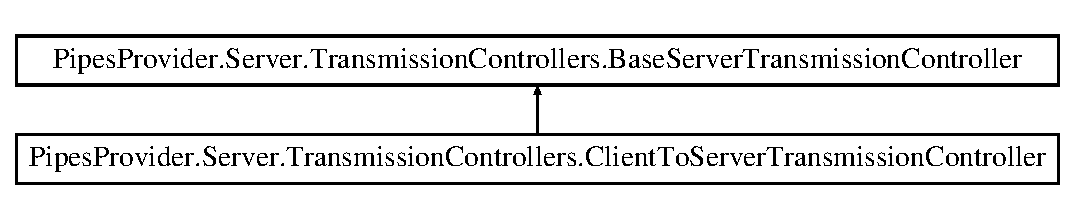
\includegraphics[height=2.000000cm]{dc/ddf/class_pipes_provider_1_1_server_1_1_transmission_controllers_1_1_client_to_server_transmission_controller}
\end{center}
\end{figure}
\subsection*{Public Member Functions}
\begin{DoxyCompactItemize}
\item 
\mbox{\Hypertarget{class_pipes_provider_1_1_server_1_1_transmission_controllers_1_1_client_to_server_transmission_controller_a74769635feb16e48b0885fac6ee29909}\label{class_pipes_provider_1_1_server_1_1_transmission_controllers_1_1_client_to_server_transmission_controller_a74769635feb16e48b0885fac6ee29909}} 
{\bfseries Client\+To\+Server\+Transmission\+Controller} (I\+Async\+Result \mbox{\hyperlink{class_pipes_provider_1_1_server_1_1_transmission_controllers_1_1_base_server_transmission_controller_afc45a2287e6fef24892a0aee8aa86f56}{connection\+Marker}}, System.\+Action$<$ \mbox{\hyperlink{class_pipes_provider_1_1_server_1_1_transmission_controllers_1_1_base_server_transmission_controller}{Base\+Server\+Transmission\+Controller}} $>$ \mbox{\hyperlink{class_pipes_provider_1_1_server_1_1_transmission_controllers_1_1_base_server_transmission_controller_a632261255d8dfc87d93445180c6e2c9d}{connection\+Callback}}, Named\+Pipe\+Server\+Stream pipe, string \mbox{\hyperlink{class_pipes_provider_1_1_server_1_1_transmission_controllers_1_1_base_server_transmission_controller_a4ce9911f1ad6814d3e5c9096d9ddde57}{pipe\+Name}})
\end{DoxyCompactItemize}
\subsection*{Static Public Member Functions}
\begin{DoxyCompactItemize}
\item 
static void \mbox{\hyperlink{class_pipes_provider_1_1_server_1_1_transmission_controllers_1_1_client_to_server_transmission_controller_a9e11d59cc7f44eee700d002df9d4f580}{Server\+Loop}} (System.\+Action$<$ \mbox{\hyperlink{class_pipes_provider_1_1_server_1_1_transmission_controllers_1_1_base_server_transmission_controller}{Base\+Server\+Transmission\+Controller}}, string $>$ \mbox{\hyperlink{class_pipes_provider_1_1_server_1_1_transmission_controllers_1_1_client_to_server_transmission_controller_a7f1552d5fea75a49edc81af944630f3e}{query\+Handler\+Callback}}, string \mbox{\hyperlink{class_pipes_provider_1_1_server_1_1_transmission_controllers_1_1_base_server_transmission_controller_a4ce9911f1ad6814d3e5c9096d9ddde57}{pipe\+Name}}, out string guid, \mbox{\hyperlink{namespace_pipes_provider_1_1_security_a1a6020eca1c661a6f7140e8260502d7e}{Security.\+Security\+Level}} security\+Level)
\begin{DoxyCompactList}\small\item\em Automaticly create server\textquotesingle{}s pipe that will recive queries from clients. \end{DoxyCompactList}\item 
static void \mbox{\hyperlink{class_pipes_provider_1_1_server_1_1_transmission_controllers_1_1_client_to_server_transmission_controller_ab52c0b0e04e34cd795847eef1e59d35b}{Server\+Loop}} (string guid, System.\+Action$<$ \mbox{\hyperlink{class_pipes_provider_1_1_server_1_1_transmission_controllers_1_1_base_server_transmission_controller}{Base\+Server\+Transmission\+Controller}}, string $>$ \mbox{\hyperlink{class_pipes_provider_1_1_server_1_1_transmission_controllers_1_1_client_to_server_transmission_controller_a7f1552d5fea75a49edc81af944630f3e}{query\+Handler\+Callback}}, string \mbox{\hyperlink{class_pipes_provider_1_1_server_1_1_transmission_controllers_1_1_base_server_transmission_controller_a4ce9911f1ad6814d3e5c9096d9ddde57}{pipe\+Name}}, \mbox{\hyperlink{namespace_pipes_provider_1_1_security_a1a6020eca1c661a6f7140e8260502d7e}{Security.\+Security\+Level}} security\+Level)
\begin{DoxyCompactList}\small\item\em Automaticly create server\textquotesingle{}s pipe. Allow to customise G\+U\+ID. \end{DoxyCompactList}\item 
static void \mbox{\hyperlink{class_pipes_provider_1_1_server_1_1_transmission_controllers_1_1_client_to_server_transmission_controller_ae66dc95c0ec1e01f53bf5d0d7e0c3738}{Server\+Loop}} (string guid, System.\+Action$<$ \mbox{\hyperlink{class_pipes_provider_1_1_server_1_1_transmission_controllers_1_1_base_server_transmission_controller}{Base\+Server\+Transmission\+Controller}}, string $>$ \mbox{\hyperlink{class_pipes_provider_1_1_server_1_1_transmission_controllers_1_1_client_to_server_transmission_controller_a7f1552d5fea75a49edc81af944630f3e}{query\+Handler\+Callback}}, string \mbox{\hyperlink{class_pipes_provider_1_1_server_1_1_transmission_controllers_1_1_base_server_transmission_controller_a4ce9911f1ad6814d3e5c9096d9ddde57}{pipe\+Name}}, int allowed\+Server\+Instances, \mbox{\hyperlink{namespace_pipes_provider_1_1_security_a1a6020eca1c661a6f7140e8260502d7e}{Security.\+Security\+Level}} security\+Level)
\begin{DoxyCompactList}\small\item\em Automaticly create server\textquotesingle{}s pipe. Allow to customise G\+U\+ID. \end{DoxyCompactList}\item 
static void \mbox{\hyperlink{class_pipes_provider_1_1_server_1_1_transmission_controllers_1_1_client_to_server_transmission_controller_abd4776718a269d7cab7ea154d94eba45}{Server\+Loop}} (string guid, System.\+Action$<$ \mbox{\hyperlink{class_pipes_provider_1_1_server_1_1_transmission_controllers_1_1_base_server_transmission_controller}{Base\+Server\+Transmission\+Controller}}, string $>$ \mbox{\hyperlink{class_pipes_provider_1_1_server_1_1_transmission_controllers_1_1_client_to_server_transmission_controller_a7f1552d5fea75a49edc81af944630f3e}{query\+Handler\+Callback}}, string \mbox{\hyperlink{class_pipes_provider_1_1_server_1_1_transmission_controllers_1_1_base_server_transmission_controller_a4ce9911f1ad6814d3e5c9096d9ddde57}{pipe\+Name}}, Pipe\+Direction pipe\+Direction, int allowed\+Server\+Instances, Pipe\+Transmission\+Mode transmission\+Mode, Pipe\+Options pipe\+Options, \mbox{\hyperlink{namespace_pipes_provider_1_1_security_a1a6020eca1c661a6f7140e8260502d7e}{Security.\+Security\+Level}} security\+Level)
\begin{DoxyCompactList}\small\item\em \mbox{\hyperlink{namespace_pipes_provider_1_1_server}{Server}} loop \end{DoxyCompactList}\end{DoxyCompactItemize}
\subsection*{Public Attributes}
\begin{DoxyCompactItemize}
\item 
System.\+Action$<$ \mbox{\hyperlink{class_pipes_provider_1_1_server_1_1_transmission_controllers_1_1_base_server_transmission_controller}{Base\+Server\+Transmission\+Controller}}, string $>$ \mbox{\hyperlink{class_pipes_provider_1_1_server_1_1_transmission_controllers_1_1_client_to_server_transmission_controller_a7f1552d5fea75a49edc81af944630f3e}{query\+Handler\+Callback}}
\begin{DoxyCompactList}\small\item\em Delegate that will be called when server will recive query. Server\+Transmission\+Meta -\/ meta data of transmission. string -\/ shared query. \end{DoxyCompactList}\end{DoxyCompactItemize}
\subsection*{Additional Inherited Members}


\subsection{Detailed Description}
Controller that provide message\textquotesingle{}s transmisssion from client to server. 



\subsection{Member Function Documentation}
\mbox{\Hypertarget{class_pipes_provider_1_1_server_1_1_transmission_controllers_1_1_client_to_server_transmission_controller_a9e11d59cc7f44eee700d002df9d4f580}\label{class_pipes_provider_1_1_server_1_1_transmission_controllers_1_1_client_to_server_transmission_controller_a9e11d59cc7f44eee700d002df9d4f580}} 
\index{Pipes\+Provider\+::\+Server\+::\+Transmission\+Controllers\+::\+Client\+To\+Server\+Transmission\+Controller@{Pipes\+Provider\+::\+Server\+::\+Transmission\+Controllers\+::\+Client\+To\+Server\+Transmission\+Controller}!Server\+Loop@{Server\+Loop}}
\index{Server\+Loop@{Server\+Loop}!Pipes\+Provider\+::\+Server\+::\+Transmission\+Controllers\+::\+Client\+To\+Server\+Transmission\+Controller@{Pipes\+Provider\+::\+Server\+::\+Transmission\+Controllers\+::\+Client\+To\+Server\+Transmission\+Controller}}
\subsubsection{\texorpdfstring{Server\+Loop()}{ServerLoop()}\hspace{0.1cm}{\footnotesize\ttfamily [1/4]}}
{\footnotesize\ttfamily static void Pipes\+Provider.\+Server.\+Transmission\+Controllers.\+Client\+To\+Server\+Transmission\+Controller.\+Server\+Loop (\begin{DoxyParamCaption}\item[{System.\+Action$<$ \mbox{\hyperlink{class_pipes_provider_1_1_server_1_1_transmission_controllers_1_1_base_server_transmission_controller}{Base\+Server\+Transmission\+Controller}}, string $>$}]{query\+Handler\+Callback,  }\item[{string}]{pipe\+Name,  }\item[{out string}]{guid,  }\item[{\mbox{\hyperlink{namespace_pipes_provider_1_1_security_a1a6020eca1c661a6f7140e8260502d7e}{Security.\+Security\+Level}}}]{security\+Level }\end{DoxyParamCaption})\hspace{0.3cm}{\ttfamily [static]}}



Automaticly create server\textquotesingle{}s pipe that will recive queries from clients. 


\begin{DoxyParams}{Parameters}
{\em query\+Handler\+Callback} & Callback that will be called when server will recive query from clinet.\\
\hline
{\em pipe\+Name} & Name of pipe that will created. \mbox{\hyperlink{namespace_pipes_provider_1_1_client}{Client}} will access this server using that name.\\
\hline
\end{DoxyParams}
\mbox{\Hypertarget{class_pipes_provider_1_1_server_1_1_transmission_controllers_1_1_client_to_server_transmission_controller_ab52c0b0e04e34cd795847eef1e59d35b}\label{class_pipes_provider_1_1_server_1_1_transmission_controllers_1_1_client_to_server_transmission_controller_ab52c0b0e04e34cd795847eef1e59d35b}} 
\index{Pipes\+Provider\+::\+Server\+::\+Transmission\+Controllers\+::\+Client\+To\+Server\+Transmission\+Controller@{Pipes\+Provider\+::\+Server\+::\+Transmission\+Controllers\+::\+Client\+To\+Server\+Transmission\+Controller}!Server\+Loop@{Server\+Loop}}
\index{Server\+Loop@{Server\+Loop}!Pipes\+Provider\+::\+Server\+::\+Transmission\+Controllers\+::\+Client\+To\+Server\+Transmission\+Controller@{Pipes\+Provider\+::\+Server\+::\+Transmission\+Controllers\+::\+Client\+To\+Server\+Transmission\+Controller}}
\subsubsection{\texorpdfstring{Server\+Loop()}{ServerLoop()}\hspace{0.1cm}{\footnotesize\ttfamily [2/4]}}
{\footnotesize\ttfamily static void Pipes\+Provider.\+Server.\+Transmission\+Controllers.\+Client\+To\+Server\+Transmission\+Controller.\+Server\+Loop (\begin{DoxyParamCaption}\item[{string}]{guid,  }\item[{System.\+Action$<$ \mbox{\hyperlink{class_pipes_provider_1_1_server_1_1_transmission_controllers_1_1_base_server_transmission_controller}{Base\+Server\+Transmission\+Controller}}, string $>$}]{query\+Handler\+Callback,  }\item[{string}]{pipe\+Name,  }\item[{\mbox{\hyperlink{namespace_pipes_provider_1_1_security_a1a6020eca1c661a6f7140e8260502d7e}{Security.\+Security\+Level}}}]{security\+Level }\end{DoxyParamCaption})\hspace{0.3cm}{\ttfamily [static]}}



Automaticly create server\textquotesingle{}s pipe. Allow to customise G\+U\+ID. 


\begin{DoxyParams}{Parameters}
{\em guid} & \\
\hline
{\em query\+Handler\+Callback} & \\
\hline
{\em pipe\+Name} & \\
\hline
\end{DoxyParams}
\mbox{\Hypertarget{class_pipes_provider_1_1_server_1_1_transmission_controllers_1_1_client_to_server_transmission_controller_ae66dc95c0ec1e01f53bf5d0d7e0c3738}\label{class_pipes_provider_1_1_server_1_1_transmission_controllers_1_1_client_to_server_transmission_controller_ae66dc95c0ec1e01f53bf5d0d7e0c3738}} 
\index{Pipes\+Provider\+::\+Server\+::\+Transmission\+Controllers\+::\+Client\+To\+Server\+Transmission\+Controller@{Pipes\+Provider\+::\+Server\+::\+Transmission\+Controllers\+::\+Client\+To\+Server\+Transmission\+Controller}!Server\+Loop@{Server\+Loop}}
\index{Server\+Loop@{Server\+Loop}!Pipes\+Provider\+::\+Server\+::\+Transmission\+Controllers\+::\+Client\+To\+Server\+Transmission\+Controller@{Pipes\+Provider\+::\+Server\+::\+Transmission\+Controllers\+::\+Client\+To\+Server\+Transmission\+Controller}}
\subsubsection{\texorpdfstring{Server\+Loop()}{ServerLoop()}\hspace{0.1cm}{\footnotesize\ttfamily [3/4]}}
{\footnotesize\ttfamily static void Pipes\+Provider.\+Server.\+Transmission\+Controllers.\+Client\+To\+Server\+Transmission\+Controller.\+Server\+Loop (\begin{DoxyParamCaption}\item[{string}]{guid,  }\item[{System.\+Action$<$ \mbox{\hyperlink{class_pipes_provider_1_1_server_1_1_transmission_controllers_1_1_base_server_transmission_controller}{Base\+Server\+Transmission\+Controller}}, string $>$}]{query\+Handler\+Callback,  }\item[{string}]{pipe\+Name,  }\item[{int}]{allowed\+Server\+Instances,  }\item[{\mbox{\hyperlink{namespace_pipes_provider_1_1_security_a1a6020eca1c661a6f7140e8260502d7e}{Security.\+Security\+Level}}}]{security\+Level }\end{DoxyParamCaption})\hspace{0.3cm}{\ttfamily [static]}}



Automaticly create server\textquotesingle{}s pipe. Allow to customise G\+U\+ID. 


\begin{DoxyParams}{Parameters}
{\em guid} & \\
\hline
{\em query\+Handler\+Callback} & \\
\hline
{\em pipe\+Name} & \\
\hline
{\em pipe\+Name} & \\
\hline
\end{DoxyParams}
\mbox{\Hypertarget{class_pipes_provider_1_1_server_1_1_transmission_controllers_1_1_client_to_server_transmission_controller_abd4776718a269d7cab7ea154d94eba45}\label{class_pipes_provider_1_1_server_1_1_transmission_controllers_1_1_client_to_server_transmission_controller_abd4776718a269d7cab7ea154d94eba45}} 
\index{Pipes\+Provider\+::\+Server\+::\+Transmission\+Controllers\+::\+Client\+To\+Server\+Transmission\+Controller@{Pipes\+Provider\+::\+Server\+::\+Transmission\+Controllers\+::\+Client\+To\+Server\+Transmission\+Controller}!Server\+Loop@{Server\+Loop}}
\index{Server\+Loop@{Server\+Loop}!Pipes\+Provider\+::\+Server\+::\+Transmission\+Controllers\+::\+Client\+To\+Server\+Transmission\+Controller@{Pipes\+Provider\+::\+Server\+::\+Transmission\+Controllers\+::\+Client\+To\+Server\+Transmission\+Controller}}
\subsubsection{\texorpdfstring{Server\+Loop()}{ServerLoop()}\hspace{0.1cm}{\footnotesize\ttfamily [4/4]}}
{\footnotesize\ttfamily static void Pipes\+Provider.\+Server.\+Transmission\+Controllers.\+Client\+To\+Server\+Transmission\+Controller.\+Server\+Loop (\begin{DoxyParamCaption}\item[{string}]{guid,  }\item[{System.\+Action$<$ \mbox{\hyperlink{class_pipes_provider_1_1_server_1_1_transmission_controllers_1_1_base_server_transmission_controller}{Base\+Server\+Transmission\+Controller}}, string $>$}]{query\+Handler\+Callback,  }\item[{string}]{pipe\+Name,  }\item[{Pipe\+Direction}]{pipe\+Direction,  }\item[{int}]{allowed\+Server\+Instances,  }\item[{Pipe\+Transmission\+Mode}]{transmission\+Mode,  }\item[{Pipe\+Options}]{pipe\+Options,  }\item[{\mbox{\hyperlink{namespace_pipes_provider_1_1_security_a1a6020eca1c661a6f7140e8260502d7e}{Security.\+Security\+Level}}}]{security\+Level }\end{DoxyParamCaption})\hspace{0.3cm}{\ttfamily [static]}}



\mbox{\hyperlink{namespace_pipes_provider_1_1_server}{Server}} loop 


\begin{DoxyParams}{Parameters}
{\em guid} & \\
\hline
{\em query\+Handler\+Callback} & \\
\hline
{\em pipe\+Name} & \\
\hline
{\em pipe\+Direction} & \\
\hline
{\em allowed\+Server\+Instances} & \\
\hline
{\em transmission\+Mode} & \\
\hline
{\em pipe\+Options} & \\
\hline
\end{DoxyParams}


\subsection{Member Data Documentation}
\mbox{\Hypertarget{class_pipes_provider_1_1_server_1_1_transmission_controllers_1_1_client_to_server_transmission_controller_a7f1552d5fea75a49edc81af944630f3e}\label{class_pipes_provider_1_1_server_1_1_transmission_controllers_1_1_client_to_server_transmission_controller_a7f1552d5fea75a49edc81af944630f3e}} 
\index{Pipes\+Provider\+::\+Server\+::\+Transmission\+Controllers\+::\+Client\+To\+Server\+Transmission\+Controller@{Pipes\+Provider\+::\+Server\+::\+Transmission\+Controllers\+::\+Client\+To\+Server\+Transmission\+Controller}!query\+Handler\+Callback@{query\+Handler\+Callback}}
\index{query\+Handler\+Callback@{query\+Handler\+Callback}!Pipes\+Provider\+::\+Server\+::\+Transmission\+Controllers\+::\+Client\+To\+Server\+Transmission\+Controller@{Pipes\+Provider\+::\+Server\+::\+Transmission\+Controllers\+::\+Client\+To\+Server\+Transmission\+Controller}}
\subsubsection{\texorpdfstring{query\+Handler\+Callback}{queryHandlerCallback}}
{\footnotesize\ttfamily System.\+Action$<$\mbox{\hyperlink{class_pipes_provider_1_1_server_1_1_transmission_controllers_1_1_base_server_transmission_controller}{Base\+Server\+Transmission\+Controller}}, string$>$ Pipes\+Provider.\+Server.\+Transmission\+Controllers.\+Client\+To\+Server\+Transmission\+Controller.\+query\+Handler\+Callback}



Delegate that will be called when server will recive query. Server\+Transmission\+Meta -\/ meta data of transmission. string -\/ shared query. 



The documentation for this class was generated from the following file\+:\begin{DoxyCompactItemize}
\item 
D\+:/\+Work/\+Git\+Hub/doloro-\/networking-\/framework/\+Pipes\+Provider/\+Server/\+Transmisssion\+Controllers/Client\+To\+Server\+Transmission\+Controller.\+cs\end{DoxyCompactItemize}

\hypertarget{class_authority_controller_1_1_a_p_i_1_1_collections}{}\section{Authority\+Controller.\+A\+P\+I.\+Collections Class Reference}
\label{class_authority_controller_1_1_a_p_i_1_1_collections}\index{Authority\+Controller.\+A\+P\+I.\+Collections@{Authority\+Controller.\+A\+P\+I.\+Collections}}


Provide \mbox{\hyperlink{namespace_authority_controller_1_1_a_p_i}{A\+PI}} to work with collection situable to authority control.  


\subsection*{Static Public Member Functions}
\begin{DoxyCompactItemize}
\item 
static bool \mbox{\hyperlink{class_authority_controller_1_1_a_p_i_1_1_collections_a7e292e3fb49b2b6f0fb1060a9beb2e9f}{Is\+Has\+Enough\+Rigths}} (string\mbox{[}$\,$\mbox{]} provided\+Rights, params string\mbox{[}$\,$\mbox{]} required\+Rights)
\begin{DoxyCompactList}\small\item\em Compare two arrays that contain rights code. Prefix \textquotesingle{}!\textquotesingle{} before rquired right will work like \char`\"{}not contain this right.\char`\"{} \end{DoxyCompactList}\item 
static bool \mbox{\hyperlink{class_authority_controller_1_1_a_p_i_1_1_collections_a65e8bd3790cb8576d37938f20dd792f4}{Ty\+Get\+Property\+Value}} (string name, out string value, params string\mbox{[}$\,$\mbox{]} properties)
\begin{DoxyCompactList}\small\item\em Loging for propery value by requested name. \end{DoxyCompactList}\end{DoxyCompactItemize}


\subsection{Detailed Description}
Provide \mbox{\hyperlink{namespace_authority_controller_1_1_a_p_i}{A\+PI}} to work with collection situable to authority control. 



\subsection{Member Function Documentation}
\mbox{\Hypertarget{class_authority_controller_1_1_a_p_i_1_1_collections_a7e292e3fb49b2b6f0fb1060a9beb2e9f}\label{class_authority_controller_1_1_a_p_i_1_1_collections_a7e292e3fb49b2b6f0fb1060a9beb2e9f}} 
\index{Authority\+Controller\+::\+A\+P\+I\+::\+Collections@{Authority\+Controller\+::\+A\+P\+I\+::\+Collections}!Is\+Has\+Enough\+Rigths@{Is\+Has\+Enough\+Rigths}}
\index{Is\+Has\+Enough\+Rigths@{Is\+Has\+Enough\+Rigths}!Authority\+Controller\+::\+A\+P\+I\+::\+Collections@{Authority\+Controller\+::\+A\+P\+I\+::\+Collections}}
\subsubsection{\texorpdfstring{Is\+Has\+Enough\+Rigths()}{IsHasEnoughRigths()}}
{\footnotesize\ttfamily static bool Authority\+Controller.\+A\+P\+I.\+Collections.\+Is\+Has\+Enough\+Rigths (\begin{DoxyParamCaption}\item[{string \mbox{[}$\,$\mbox{]}}]{provided\+Rights,  }\item[{params string \mbox{[}$\,$\mbox{]}}]{required\+Rights }\end{DoxyParamCaption})\hspace{0.3cm}{\ttfamily [static]}}



Compare two arrays that contain rights code. Prefix \textquotesingle{}!\textquotesingle{} before rquired right will work like \char`\"{}not contain this right.\char`\"{} 


\begin{DoxyParams}{Parameters}
{\em provided\+Rights} & Rights that provided to user.\\
\hline
{\em required\+Rights} & Rights that required to get permisssion.\\
\hline
\end{DoxyParams}
\begin{DoxyReturn}{Returns}

\end{DoxyReturn}
\mbox{\Hypertarget{class_authority_controller_1_1_a_p_i_1_1_collections_a65e8bd3790cb8576d37938f20dd792f4}\label{class_authority_controller_1_1_a_p_i_1_1_collections_a65e8bd3790cb8576d37938f20dd792f4}} 
\index{Authority\+Controller\+::\+A\+P\+I\+::\+Collections@{Authority\+Controller\+::\+A\+P\+I\+::\+Collections}!Ty\+Get\+Property\+Value@{Ty\+Get\+Property\+Value}}
\index{Ty\+Get\+Property\+Value@{Ty\+Get\+Property\+Value}!Authority\+Controller\+::\+A\+P\+I\+::\+Collections@{Authority\+Controller\+::\+A\+P\+I\+::\+Collections}}
\subsubsection{\texorpdfstring{Ty\+Get\+Property\+Value()}{TyGetPropertyValue()}}
{\footnotesize\ttfamily static bool Authority\+Controller.\+A\+P\+I.\+Collections.\+Ty\+Get\+Property\+Value (\begin{DoxyParamCaption}\item[{string}]{name,  }\item[{out string}]{value,  }\item[{params string \mbox{[}$\,$\mbox{]}}]{properties }\end{DoxyParamCaption})\hspace{0.3cm}{\ttfamily [static]}}



Loging for propery value by requested name. 


\begin{DoxyParams}{Parameters}
{\em name} & \\
\hline
{\em value} & Value that stored to that property by using \char`\"{}\+P\+R\+O\+P\+\_\+\+N\+A\+M\+E=\+P\+R\+O\+P\+\_\+\+V\+A\+L\+U\+E\char`\"{} format. N\+U\+LL if empty.\\
\hline
{\em properties} & Array that contain properties\textquotesingle{} collection.\\
\hline
\end{DoxyParams}
\begin{DoxyReturn}{Returns}
Result of the seeking.
\end{DoxyReturn}


The documentation for this class was generated from the following file\+:\begin{DoxyCompactItemize}
\item 
D\+:/\+Work/\+Git\+Hub/doloro-\/networking-\/framework/\+Authority\+Controller/\+A\+P\+I/Collections.\+cs\end{DoxyCompactItemize}

\hypertarget{class_uniform_server_1_1_commands}{}\section{Uniform\+Server.\+Commands Class Reference}
\label{class_uniform_server_1_1_commands}\index{Uniform\+Server.\+Commands@{Uniform\+Server.\+Commands}}
\subsection*{Static Public Member Functions}
\begin{DoxyCompactItemize}
\item 
static bool \mbox{\hyperlink{class_uniform_server_1_1_commands_ad1bac97da40d03e97f9b5fe7ed152ef9}{Base\+Commands}} (string command)
\begin{DoxyCompactList}\small\item\em React to the base commands that can be applied to every server. \end{DoxyCompactList}\end{DoxyCompactItemize}


\subsection{Member Function Documentation}
\mbox{\Hypertarget{class_uniform_server_1_1_commands_ad1bac97da40d03e97f9b5fe7ed152ef9}\label{class_uniform_server_1_1_commands_ad1bac97da40d03e97f9b5fe7ed152ef9}} 
\index{Uniform\+Server\+::\+Commands@{Uniform\+Server\+::\+Commands}!Base\+Commands@{Base\+Commands}}
\index{Base\+Commands@{Base\+Commands}!Uniform\+Server\+::\+Commands@{Uniform\+Server\+::\+Commands}}
\subsubsection{\texorpdfstring{Base\+Commands()}{BaseCommands()}}
{\footnotesize\ttfamily static bool Uniform\+Server.\+Commands.\+Base\+Commands (\begin{DoxyParamCaption}\item[{string}]{command }\end{DoxyParamCaption})\hspace{0.3cm}{\ttfamily [static]}}



React to the base commands that can be applied to every server. 


\begin{DoxyParams}{Parameters}
{\em command} & \\
\hline
\end{DoxyParams}


The documentation for this class was generated from the following file\+:\begin{DoxyCompactItemize}
\item 
D\+:/\+Work/\+Git\+Hub/doloro-\/networking-\/framework/\+Core/\+D\+N\+F\+Core/\+Uniform\+Server/\+Application/Commands.\+cs\end{DoxyCompactItemize}

\hypertarget{class_authority_controller_1_1_data_1_1_application_1_1_config}{}\section{Authority\+Controller.\+Data.\+Application.\+Config Class Reference}
\label{class_authority_controller_1_1_data_1_1_application_1_1_config}\index{Authority\+Controller.\+Data.\+Application.\+Config@{Authority\+Controller.\+Data.\+Application.\+Config}}


Object that contain data for setup of authority controller.  


\subsection*{Public Attributes}
\begin{DoxyCompactItemize}
\item 
string \mbox{\hyperlink{class_authority_controller_1_1_data_1_1_application_1_1_config_a9889d48151e034f0bc451126058a5264}{Users\+Storage\+Directory}} = \char`\"{}\textbackslash{}\textbackslash{}resorces\textbackslash{}\textbackslash{}users\textbackslash{}\textbackslash{}\char`\"{}
\begin{DoxyCompactList}\small\item\em Directory to folder that will contain users data. \end{DoxyCompactList}\item 
int \mbox{\hyperlink{class_authority_controller_1_1_data_1_1_application_1_1_config_a0cdcdcfb29481fdcd78202203d10d53c}{Login\+Min\+Size}} = 5
\begin{DoxyCompactList}\small\item\em How many character will be required in password. \end{DoxyCompactList}\item 
int \mbox{\hyperlink{class_authority_controller_1_1_data_1_1_application_1_1_config_a0ad628b23000c825b59e4755c10e70fe}{Login\+Max\+Size}} = 16
\begin{DoxyCompactList}\small\item\em How many character will be allowed in password. \end{DoxyCompactList}\item 
string \mbox{\hyperlink{class_authority_controller_1_1_data_1_1_application_1_1_config_a91b4d10af2d9680e0580c5fe30b09fc8}{User\+Name\+Regex\+Pattern}} = @\char`\"{}$^\wedge$(\mbox{[}A-\/Z\mbox{]}\mbox{[}a-\/z\mbox{]}+)+(\mbox{[}-\/\textquotesingle{} \mbox{]}\mbox{[}A-\/Z\mbox{]}\mbox{[}a-\/z\mbox{]}+)?\$\char`\"{}
\begin{DoxyCompactList}\small\item\em Define a format of allowed name. By default provide possibility to make a names like\+: X\+X\+X\+XX Xxxx-\/\+Xxxx Xx\textquotesingle{}Xxx etc. \end{DoxyCompactList}\item 
string \mbox{[}$\,$\mbox{]} \mbox{\hyperlink{class_authority_controller_1_1_data_1_1_application_1_1_config_a4f98440aff22ba7124faf929df4401ba}{User\+Default\+Rights}}
\begin{DoxyCompactList}\small\item\em List of user rights that will profided to every new user. Any extra rights will require aditional query from authorised user. \end{DoxyCompactList}\item 
string \mbox{\hyperlink{class_authority_controller_1_1_data_1_1_application_1_1_config_af2c4e3d6eba2ff61eed570390bfdcc14}{Password\+Salt\+File\+Name}} = \char`\"{}.salt\char`\"{}
\begin{DoxyCompactList}\small\item\em Name of the file that will contain salt. \end{DoxyCompactList}\item 
int \mbox{\hyperlink{class_authority_controller_1_1_data_1_1_application_1_1_config_a0b7dd2a319692cc608de89f4a463cb61}{Password\+Salt\+Size}} = 32
\begin{DoxyCompactList}\small\item\em How many bytes will contain salt. \end{DoxyCompactList}\item 
int \mbox{\hyperlink{class_authority_controller_1_1_data_1_1_application_1_1_config_ac6d18cfffc86aaa2443a06a90a688eb1}{Password\+Min\+Allowed\+Length}} = 8
\begin{DoxyCompactList}\small\item\em How many character will be required in password. \end{DoxyCompactList}\item 
int \mbox{\hyperlink{class_authority_controller_1_1_data_1_1_application_1_1_config_a04f768eacbc58e94bd7f5122eaf659fb}{Password\+Max\+Allowed\+Length}} = 32
\begin{DoxyCompactList}\small\item\em How many character will be allowed in password. \end{DoxyCompactList}\item 
bool \mbox{\hyperlink{class_authority_controller_1_1_data_1_1_application_1_1_config_ae20771ce3750b078895ef998a57d8773}{Password\+Require\+Special\+Symbol}} = false
\begin{DoxyCompactList}\small\item\em If true then will requre at leas one symbol like !\$\% etc. \mbox{\hyperlink{namespace_authority_controller_1_1_data_1_1_application}{Application}} will provide valid mask without your involving. \end{DoxyCompactList}\item 
bool \mbox{\hyperlink{class_authority_controller_1_1_data_1_1_application_1_1_config_a8ac9eca1d9766ddc46f9177133dd8b6e}{Password\+Require\+Upper\+Symbol}} = true
\begin{DoxyCompactList}\small\item\em If true then will require at least one symbol in high register. \mbox{\hyperlink{namespace_authority_controller_1_1_data_1_1_application}{Application}} will provide valid mask without your involving. \end{DoxyCompactList}\item 
bool \mbox{\hyperlink{class_authority_controller_1_1_data_1_1_application_1_1_config_a2f39b6a13a99fc5a433d333b086fdcad}{Password\+Require\+Digit\+Symbol}} = true
\begin{DoxyCompactList}\small\item\em If true then will require at least one digit. \mbox{\hyperlink{namespace_authority_controller_1_1_data_1_1_application}{Application}} will provide valid mask without your involving. \end{DoxyCompactList}\item 
int \mbox{\hyperlink{class_authority_controller_1_1_data_1_1_application_1_1_config_ad548f5fee544802b6c900eef6da88332}{Token\+Valid\+Time\+Minutes}} = 1440
\begin{DoxyCompactList}\small\item\em How many minutes token is valid. \end{DoxyCompactList}\item 
string \mbox{[}$\,$\mbox{]} \mbox{\hyperlink{class_authority_controller_1_1_data_1_1_application_1_1_config_a6d369c29beecb9c80a65168d72e2ae06}{Q\+U\+E\+R\+Y\+\_\+\+User\+Ban\+\_\+\+R\+I\+G\+H\+TS}} = new string\mbox{[}$\,$\mbox{]} \{ \char`\"{}banhammer\char`\"{}, \char`\"{}$>$rank=2\char`\"{} \}
\begin{DoxyCompactList}\small\item\em Rights code required for requester to proceed this action. \end{DoxyCompactList}\item 
string \mbox{[}$\,$\mbox{]} \mbox{\hyperlink{class_authority_controller_1_1_data_1_1_application_1_1_config_a93960243b140fa132aef425493c7bb70}{Q\+U\+E\+R\+Y\+\_\+\+User\+New\+Password\+\_\+\+R\+I\+G\+H\+TS}} = new string\mbox{[}$\,$\mbox{]} \{ \char`\"{}password\+Managing\char`\"{} \}
\begin{DoxyCompactList}\small\item\em Rights code required for requester to proceed this action. \end{DoxyCompactList}\item 
string \mbox{[}$\,$\mbox{]} \mbox{\hyperlink{class_authority_controller_1_1_data_1_1_application_1_1_config_acf5f9058d36f7fd7fb017098481f8dfc}{Q\+U\+E\+R\+Y\+\_\+\+User\+Password\+Moderation\+\_\+\+R\+I\+G\+H\+TS}} = new string\mbox{[}$\,$\mbox{]} \{ \char`\"{}$>$rank=2\char`\"{} \}
\begin{DoxyCompactList}\small\item\em What a rights will required to user that try to change the password of other user. Also system auto add instruction where user need to have hieghest rank the target. \end{DoxyCompactList}\item 
string \mbox{[}$\,$\mbox{]} \mbox{\hyperlink{class_authority_controller_1_1_data_1_1_application_1_1_config_a0ac15c9d4920092355022d3cc0d47f4d}{Q\+U\+E\+R\+Y\+\_\+\+Set\+Token\+Rights\+\_\+\+R\+I\+G\+H\+TS}} = new string\mbox{[}$\,$\mbox{]} \{\char`\"{}$>$rank=5\char`\"{} \}
\begin{DoxyCompactList}\small\item\em Rights code required for requester to proceed this action. $>$rank=4 -\/ will requre at least admin level. \end{DoxyCompactList}\end{DoxyCompactItemize}
\subsection*{Static Public Attributes}
\begin{DoxyCompactItemize}
\item 
static string \mbox{\hyperlink{class_authority_controller_1_1_data_1_1_application_1_1_config_ad3be522aa76fea2a368ffa3810979012}{D\+I\+R\+E\+C\+T\+O\+RY}} = \char`\"{}\textbackslash{}\textbackslash{}resources\textbackslash{}\textbackslash{}ac\textbackslash{}\textbackslash{}\char`\"{}
\begin{DoxyCompactList}\small\item\em Directory that will contain serialized instance of this class. \end{DoxyCompactList}\item 
static string \mbox{\hyperlink{class_authority_controller_1_1_data_1_1_application_1_1_config_a7cc94e6fe35ce997e75f0a0fa3feaa2e}{C\+O\+N\+F\+I\+G\+\_\+\+F\+I\+L\+E\+\_\+\+N\+A\+ME}} = \char`\"{}.config\char`\"{}
\begin{DoxyCompactList}\small\item\em Name of the file that will be loaded as config. \end{DoxyCompactList}\end{DoxyCompactItemize}
\subsection*{Properties}
\begin{DoxyCompactItemize}
\item 
static \mbox{\hyperlink{class_authority_controller_1_1_data_1_1_application_1_1_config}{Config}} \mbox{\hyperlink{class_authority_controller_1_1_data_1_1_application_1_1_config_a4473b20e9b91d2811ac3610da497a1bc}{Active}}\hspace{0.3cm}{\ttfamily  \mbox{[}get, set\mbox{]}}
\begin{DoxyCompactList}\small\item\em Reference to current configs. Auto load one from resources if exist by D\+I\+R\+E\+C\+T\+O\+RY. \end{DoxyCompactList}\item 
\mbox{\hyperlink{class_authority_controller_1_1_data_1_1_application_1_1_salt_container}{Salt\+Container}} \mbox{\hyperlink{class_authority_controller_1_1_data_1_1_application_1_1_config_ac91189185d3ab6bf689bfaf37f83d9c1}{Salt}}\hspace{0.3cm}{\ttfamily  \mbox{[}get\mbox{]}}
\begin{DoxyCompactList}\small\item\em Salt loaded from file. \end{DoxyCompactList}\end{DoxyCompactItemize}
\subsection*{Private Attributes}
\begin{DoxyCompactItemize}
\item 
\mbox{\Hypertarget{class_authority_controller_1_1_data_1_1_application_1_1_config_abcf55c74cb4f50ee8a68e53a2f1fbf4c}\label{class_authority_controller_1_1_data_1_1_application_1_1_config_abcf55c74cb4f50ee8a68e53a2f1fbf4c}} 
\mbox{\hyperlink{class_authority_controller_1_1_data_1_1_application_1_1_salt_container}{Salt\+Container}} {\bfseries salt}
\end{DoxyCompactItemize}
\subsection*{Static Private Attributes}
\begin{DoxyCompactItemize}
\item 
\mbox{\Hypertarget{class_authority_controller_1_1_data_1_1_application_1_1_config_a889d164fa5479754663de6c2d64983ba}\label{class_authority_controller_1_1_data_1_1_application_1_1_config_a889d164fa5479754663de6c2d64983ba}} 
static \mbox{\hyperlink{class_authority_controller_1_1_data_1_1_application_1_1_config}{Config}} {\bfseries active}
\end{DoxyCompactItemize}


\subsection{Detailed Description}
Object that contain data for setup of authority controller. 



\subsection{Member Data Documentation}
\mbox{\Hypertarget{class_authority_controller_1_1_data_1_1_application_1_1_config_a7cc94e6fe35ce997e75f0a0fa3feaa2e}\label{class_authority_controller_1_1_data_1_1_application_1_1_config_a7cc94e6fe35ce997e75f0a0fa3feaa2e}} 
\index{Authority\+Controller\+::\+Data\+::\+Application\+::\+Config@{Authority\+Controller\+::\+Data\+::\+Application\+::\+Config}!C\+O\+N\+F\+I\+G\+\_\+\+F\+I\+L\+E\+\_\+\+N\+A\+ME@{C\+O\+N\+F\+I\+G\+\_\+\+F\+I\+L\+E\+\_\+\+N\+A\+ME}}
\index{C\+O\+N\+F\+I\+G\+\_\+\+F\+I\+L\+E\+\_\+\+N\+A\+ME@{C\+O\+N\+F\+I\+G\+\_\+\+F\+I\+L\+E\+\_\+\+N\+A\+ME}!Authority\+Controller\+::\+Data\+::\+Application\+::\+Config@{Authority\+Controller\+::\+Data\+::\+Application\+::\+Config}}
\subsubsection{\texorpdfstring{C\+O\+N\+F\+I\+G\+\_\+\+F\+I\+L\+E\+\_\+\+N\+A\+ME}{CONFIG\_FILE\_NAME}}
{\footnotesize\ttfamily string Authority\+Controller.\+Data.\+Application.\+Config.\+C\+O\+N\+F\+I\+G\+\_\+\+F\+I\+L\+E\+\_\+\+N\+A\+ME = \char`\"{}.config\char`\"{}\hspace{0.3cm}{\ttfamily [static]}}



Name of the file that will be loaded as config. 

\mbox{\Hypertarget{class_authority_controller_1_1_data_1_1_application_1_1_config_ad3be522aa76fea2a368ffa3810979012}\label{class_authority_controller_1_1_data_1_1_application_1_1_config_ad3be522aa76fea2a368ffa3810979012}} 
\index{Authority\+Controller\+::\+Data\+::\+Application\+::\+Config@{Authority\+Controller\+::\+Data\+::\+Application\+::\+Config}!D\+I\+R\+E\+C\+T\+O\+RY@{D\+I\+R\+E\+C\+T\+O\+RY}}
\index{D\+I\+R\+E\+C\+T\+O\+RY@{D\+I\+R\+E\+C\+T\+O\+RY}!Authority\+Controller\+::\+Data\+::\+Application\+::\+Config@{Authority\+Controller\+::\+Data\+::\+Application\+::\+Config}}
\subsubsection{\texorpdfstring{D\+I\+R\+E\+C\+T\+O\+RY}{DIRECTORY}}
{\footnotesize\ttfamily string Authority\+Controller.\+Data.\+Application.\+Config.\+D\+I\+R\+E\+C\+T\+O\+RY = \char`\"{}\textbackslash{}\textbackslash{}resources\textbackslash{}\textbackslash{}ac\textbackslash{}\textbackslash{}\char`\"{}\hspace{0.3cm}{\ttfamily [static]}}



Directory that will contain serialized instance of this class. 

\mbox{\Hypertarget{class_authority_controller_1_1_data_1_1_application_1_1_config_a0ad628b23000c825b59e4755c10e70fe}\label{class_authority_controller_1_1_data_1_1_application_1_1_config_a0ad628b23000c825b59e4755c10e70fe}} 
\index{Authority\+Controller\+::\+Data\+::\+Application\+::\+Config@{Authority\+Controller\+::\+Data\+::\+Application\+::\+Config}!Login\+Max\+Size@{Login\+Max\+Size}}
\index{Login\+Max\+Size@{Login\+Max\+Size}!Authority\+Controller\+::\+Data\+::\+Application\+::\+Config@{Authority\+Controller\+::\+Data\+::\+Application\+::\+Config}}
\subsubsection{\texorpdfstring{Login\+Max\+Size}{LoginMaxSize}}
{\footnotesize\ttfamily int Authority\+Controller.\+Data.\+Application.\+Config.\+Login\+Max\+Size = 16}



How many character will be allowed in password. 

\mbox{\Hypertarget{class_authority_controller_1_1_data_1_1_application_1_1_config_a0cdcdcfb29481fdcd78202203d10d53c}\label{class_authority_controller_1_1_data_1_1_application_1_1_config_a0cdcdcfb29481fdcd78202203d10d53c}} 
\index{Authority\+Controller\+::\+Data\+::\+Application\+::\+Config@{Authority\+Controller\+::\+Data\+::\+Application\+::\+Config}!Login\+Min\+Size@{Login\+Min\+Size}}
\index{Login\+Min\+Size@{Login\+Min\+Size}!Authority\+Controller\+::\+Data\+::\+Application\+::\+Config@{Authority\+Controller\+::\+Data\+::\+Application\+::\+Config}}
\subsubsection{\texorpdfstring{Login\+Min\+Size}{LoginMinSize}}
{\footnotesize\ttfamily int Authority\+Controller.\+Data.\+Application.\+Config.\+Login\+Min\+Size = 5}



How many character will be required in password. 

\mbox{\Hypertarget{class_authority_controller_1_1_data_1_1_application_1_1_config_a04f768eacbc58e94bd7f5122eaf659fb}\label{class_authority_controller_1_1_data_1_1_application_1_1_config_a04f768eacbc58e94bd7f5122eaf659fb}} 
\index{Authority\+Controller\+::\+Data\+::\+Application\+::\+Config@{Authority\+Controller\+::\+Data\+::\+Application\+::\+Config}!Password\+Max\+Allowed\+Length@{Password\+Max\+Allowed\+Length}}
\index{Password\+Max\+Allowed\+Length@{Password\+Max\+Allowed\+Length}!Authority\+Controller\+::\+Data\+::\+Application\+::\+Config@{Authority\+Controller\+::\+Data\+::\+Application\+::\+Config}}
\subsubsection{\texorpdfstring{Password\+Max\+Allowed\+Length}{PasswordMaxAllowedLength}}
{\footnotesize\ttfamily int Authority\+Controller.\+Data.\+Application.\+Config.\+Password\+Max\+Allowed\+Length = 32}



How many character will be allowed in password. 

\mbox{\Hypertarget{class_authority_controller_1_1_data_1_1_application_1_1_config_ac6d18cfffc86aaa2443a06a90a688eb1}\label{class_authority_controller_1_1_data_1_1_application_1_1_config_ac6d18cfffc86aaa2443a06a90a688eb1}} 
\index{Authority\+Controller\+::\+Data\+::\+Application\+::\+Config@{Authority\+Controller\+::\+Data\+::\+Application\+::\+Config}!Password\+Min\+Allowed\+Length@{Password\+Min\+Allowed\+Length}}
\index{Password\+Min\+Allowed\+Length@{Password\+Min\+Allowed\+Length}!Authority\+Controller\+::\+Data\+::\+Application\+::\+Config@{Authority\+Controller\+::\+Data\+::\+Application\+::\+Config}}
\subsubsection{\texorpdfstring{Password\+Min\+Allowed\+Length}{PasswordMinAllowedLength}}
{\footnotesize\ttfamily int Authority\+Controller.\+Data.\+Application.\+Config.\+Password\+Min\+Allowed\+Length = 8}



How many character will be required in password. 

\mbox{\Hypertarget{class_authority_controller_1_1_data_1_1_application_1_1_config_a2f39b6a13a99fc5a433d333b086fdcad}\label{class_authority_controller_1_1_data_1_1_application_1_1_config_a2f39b6a13a99fc5a433d333b086fdcad}} 
\index{Authority\+Controller\+::\+Data\+::\+Application\+::\+Config@{Authority\+Controller\+::\+Data\+::\+Application\+::\+Config}!Password\+Require\+Digit\+Symbol@{Password\+Require\+Digit\+Symbol}}
\index{Password\+Require\+Digit\+Symbol@{Password\+Require\+Digit\+Symbol}!Authority\+Controller\+::\+Data\+::\+Application\+::\+Config@{Authority\+Controller\+::\+Data\+::\+Application\+::\+Config}}
\subsubsection{\texorpdfstring{Password\+Require\+Digit\+Symbol}{PasswordRequireDigitSymbol}}
{\footnotesize\ttfamily bool Authority\+Controller.\+Data.\+Application.\+Config.\+Password\+Require\+Digit\+Symbol = true}



If true then will require at least one digit. \mbox{\hyperlink{namespace_authority_controller_1_1_data_1_1_application}{Application}} will provide valid mask without your involving. 

\mbox{\Hypertarget{class_authority_controller_1_1_data_1_1_application_1_1_config_ae20771ce3750b078895ef998a57d8773}\label{class_authority_controller_1_1_data_1_1_application_1_1_config_ae20771ce3750b078895ef998a57d8773}} 
\index{Authority\+Controller\+::\+Data\+::\+Application\+::\+Config@{Authority\+Controller\+::\+Data\+::\+Application\+::\+Config}!Password\+Require\+Special\+Symbol@{Password\+Require\+Special\+Symbol}}
\index{Password\+Require\+Special\+Symbol@{Password\+Require\+Special\+Symbol}!Authority\+Controller\+::\+Data\+::\+Application\+::\+Config@{Authority\+Controller\+::\+Data\+::\+Application\+::\+Config}}
\subsubsection{\texorpdfstring{Password\+Require\+Special\+Symbol}{PasswordRequireSpecialSymbol}}
{\footnotesize\ttfamily bool Authority\+Controller.\+Data.\+Application.\+Config.\+Password\+Require\+Special\+Symbol = false}



If true then will requre at leas one symbol like !\$\% etc. \mbox{\hyperlink{namespace_authority_controller_1_1_data_1_1_application}{Application}} will provide valid mask without your involving. 

\mbox{\Hypertarget{class_authority_controller_1_1_data_1_1_application_1_1_config_a8ac9eca1d9766ddc46f9177133dd8b6e}\label{class_authority_controller_1_1_data_1_1_application_1_1_config_a8ac9eca1d9766ddc46f9177133dd8b6e}} 
\index{Authority\+Controller\+::\+Data\+::\+Application\+::\+Config@{Authority\+Controller\+::\+Data\+::\+Application\+::\+Config}!Password\+Require\+Upper\+Symbol@{Password\+Require\+Upper\+Symbol}}
\index{Password\+Require\+Upper\+Symbol@{Password\+Require\+Upper\+Symbol}!Authority\+Controller\+::\+Data\+::\+Application\+::\+Config@{Authority\+Controller\+::\+Data\+::\+Application\+::\+Config}}
\subsubsection{\texorpdfstring{Password\+Require\+Upper\+Symbol}{PasswordRequireUpperSymbol}}
{\footnotesize\ttfamily bool Authority\+Controller.\+Data.\+Application.\+Config.\+Password\+Require\+Upper\+Symbol = true}



If true then will require at least one symbol in high register. \mbox{\hyperlink{namespace_authority_controller_1_1_data_1_1_application}{Application}} will provide valid mask without your involving. 

\mbox{\Hypertarget{class_authority_controller_1_1_data_1_1_application_1_1_config_af2c4e3d6eba2ff61eed570390bfdcc14}\label{class_authority_controller_1_1_data_1_1_application_1_1_config_af2c4e3d6eba2ff61eed570390bfdcc14}} 
\index{Authority\+Controller\+::\+Data\+::\+Application\+::\+Config@{Authority\+Controller\+::\+Data\+::\+Application\+::\+Config}!Password\+Salt\+File\+Name@{Password\+Salt\+File\+Name}}
\index{Password\+Salt\+File\+Name@{Password\+Salt\+File\+Name}!Authority\+Controller\+::\+Data\+::\+Application\+::\+Config@{Authority\+Controller\+::\+Data\+::\+Application\+::\+Config}}
\subsubsection{\texorpdfstring{Password\+Salt\+File\+Name}{PasswordSaltFileName}}
{\footnotesize\ttfamily string Authority\+Controller.\+Data.\+Application.\+Config.\+Password\+Salt\+File\+Name = \char`\"{}.salt\char`\"{}}



Name of the file that will contain salt. 

\mbox{\Hypertarget{class_authority_controller_1_1_data_1_1_application_1_1_config_a0b7dd2a319692cc608de89f4a463cb61}\label{class_authority_controller_1_1_data_1_1_application_1_1_config_a0b7dd2a319692cc608de89f4a463cb61}} 
\index{Authority\+Controller\+::\+Data\+::\+Application\+::\+Config@{Authority\+Controller\+::\+Data\+::\+Application\+::\+Config}!Password\+Salt\+Size@{Password\+Salt\+Size}}
\index{Password\+Salt\+Size@{Password\+Salt\+Size}!Authority\+Controller\+::\+Data\+::\+Application\+::\+Config@{Authority\+Controller\+::\+Data\+::\+Application\+::\+Config}}
\subsubsection{\texorpdfstring{Password\+Salt\+Size}{PasswordSaltSize}}
{\footnotesize\ttfamily int Authority\+Controller.\+Data.\+Application.\+Config.\+Password\+Salt\+Size = 32}



How many bytes will contain salt. 

\mbox{\Hypertarget{class_authority_controller_1_1_data_1_1_application_1_1_config_a0ac15c9d4920092355022d3cc0d47f4d}\label{class_authority_controller_1_1_data_1_1_application_1_1_config_a0ac15c9d4920092355022d3cc0d47f4d}} 
\index{Authority\+Controller\+::\+Data\+::\+Application\+::\+Config@{Authority\+Controller\+::\+Data\+::\+Application\+::\+Config}!Q\+U\+E\+R\+Y\+\_\+\+Set\+Token\+Rights\+\_\+\+R\+I\+G\+H\+TS@{Q\+U\+E\+R\+Y\+\_\+\+Set\+Token\+Rights\+\_\+\+R\+I\+G\+H\+TS}}
\index{Q\+U\+E\+R\+Y\+\_\+\+Set\+Token\+Rights\+\_\+\+R\+I\+G\+H\+TS@{Q\+U\+E\+R\+Y\+\_\+\+Set\+Token\+Rights\+\_\+\+R\+I\+G\+H\+TS}!Authority\+Controller\+::\+Data\+::\+Application\+::\+Config@{Authority\+Controller\+::\+Data\+::\+Application\+::\+Config}}
\subsubsection{\texorpdfstring{Q\+U\+E\+R\+Y\+\_\+\+Set\+Token\+Rights\+\_\+\+R\+I\+G\+H\+TS}{QUERY\_SetTokenRights\_RIGHTS}}
{\footnotesize\ttfamily string \mbox{[}$\,$\mbox{]} Authority\+Controller.\+Data.\+Application.\+Config.\+Q\+U\+E\+R\+Y\+\_\+\+Set\+Token\+Rights\+\_\+\+R\+I\+G\+H\+TS = new string\mbox{[}$\,$\mbox{]} \{\char`\"{}$>$rank=5\char`\"{} \}}



Rights code required for requester to proceed this action. $>$rank=4 -\/ will requre at least admin level. 

\mbox{\Hypertarget{class_authority_controller_1_1_data_1_1_application_1_1_config_a6d369c29beecb9c80a65168d72e2ae06}\label{class_authority_controller_1_1_data_1_1_application_1_1_config_a6d369c29beecb9c80a65168d72e2ae06}} 
\index{Authority\+Controller\+::\+Data\+::\+Application\+::\+Config@{Authority\+Controller\+::\+Data\+::\+Application\+::\+Config}!Q\+U\+E\+R\+Y\+\_\+\+User\+Ban\+\_\+\+R\+I\+G\+H\+TS@{Q\+U\+E\+R\+Y\+\_\+\+User\+Ban\+\_\+\+R\+I\+G\+H\+TS}}
\index{Q\+U\+E\+R\+Y\+\_\+\+User\+Ban\+\_\+\+R\+I\+G\+H\+TS@{Q\+U\+E\+R\+Y\+\_\+\+User\+Ban\+\_\+\+R\+I\+G\+H\+TS}!Authority\+Controller\+::\+Data\+::\+Application\+::\+Config@{Authority\+Controller\+::\+Data\+::\+Application\+::\+Config}}
\subsubsection{\texorpdfstring{Q\+U\+E\+R\+Y\+\_\+\+User\+Ban\+\_\+\+R\+I\+G\+H\+TS}{QUERY\_UserBan\_RIGHTS}}
{\footnotesize\ttfamily string \mbox{[}$\,$\mbox{]} Authority\+Controller.\+Data.\+Application.\+Config.\+Q\+U\+E\+R\+Y\+\_\+\+User\+Ban\+\_\+\+R\+I\+G\+H\+TS = new string\mbox{[}$\,$\mbox{]} \{ \char`\"{}banhammer\char`\"{}, \char`\"{}$>$rank=2\char`\"{} \}}



Rights code required for requester to proceed this action. 

rank=x where x is 0 -\/ guest 1 -\/ user 2 -\/ privileged user 4 -\/ moderator 8 -\/ admin 16 -\/ superadminbannhammer -\/ allow user set bans to others. $>$rank=2 -\/ wil requre at least moderators level. \mbox{\Hypertarget{class_authority_controller_1_1_data_1_1_application_1_1_config_a93960243b140fa132aef425493c7bb70}\label{class_authority_controller_1_1_data_1_1_application_1_1_config_a93960243b140fa132aef425493c7bb70}} 
\index{Authority\+Controller\+::\+Data\+::\+Application\+::\+Config@{Authority\+Controller\+::\+Data\+::\+Application\+::\+Config}!Q\+U\+E\+R\+Y\+\_\+\+User\+New\+Password\+\_\+\+R\+I\+G\+H\+TS@{Q\+U\+E\+R\+Y\+\_\+\+User\+New\+Password\+\_\+\+R\+I\+G\+H\+TS}}
\index{Q\+U\+E\+R\+Y\+\_\+\+User\+New\+Password\+\_\+\+R\+I\+G\+H\+TS@{Q\+U\+E\+R\+Y\+\_\+\+User\+New\+Password\+\_\+\+R\+I\+G\+H\+TS}!Authority\+Controller\+::\+Data\+::\+Application\+::\+Config@{Authority\+Controller\+::\+Data\+::\+Application\+::\+Config}}
\subsubsection{\texorpdfstring{Q\+U\+E\+R\+Y\+\_\+\+User\+New\+Password\+\_\+\+R\+I\+G\+H\+TS}{QUERY\_UserNewPassword\_RIGHTS}}
{\footnotesize\ttfamily string \mbox{[}$\,$\mbox{]} Authority\+Controller.\+Data.\+Application.\+Config.\+Q\+U\+E\+R\+Y\+\_\+\+User\+New\+Password\+\_\+\+R\+I\+G\+H\+TS = new string\mbox{[}$\,$\mbox{]} \{ \char`\"{}password\+Managing\char`\"{} \}}



Rights code required for requester to proceed this action. 

password\+Managing -\/ user can change them passwords. \mbox{\Hypertarget{class_authority_controller_1_1_data_1_1_application_1_1_config_acf5f9058d36f7fd7fb017098481f8dfc}\label{class_authority_controller_1_1_data_1_1_application_1_1_config_acf5f9058d36f7fd7fb017098481f8dfc}} 
\index{Authority\+Controller\+::\+Data\+::\+Application\+::\+Config@{Authority\+Controller\+::\+Data\+::\+Application\+::\+Config}!Q\+U\+E\+R\+Y\+\_\+\+User\+Password\+Moderation\+\_\+\+R\+I\+G\+H\+TS@{Q\+U\+E\+R\+Y\+\_\+\+User\+Password\+Moderation\+\_\+\+R\+I\+G\+H\+TS}}
\index{Q\+U\+E\+R\+Y\+\_\+\+User\+Password\+Moderation\+\_\+\+R\+I\+G\+H\+TS@{Q\+U\+E\+R\+Y\+\_\+\+User\+Password\+Moderation\+\_\+\+R\+I\+G\+H\+TS}!Authority\+Controller\+::\+Data\+::\+Application\+::\+Config@{Authority\+Controller\+::\+Data\+::\+Application\+::\+Config}}
\subsubsection{\texorpdfstring{Q\+U\+E\+R\+Y\+\_\+\+User\+Password\+Moderation\+\_\+\+R\+I\+G\+H\+TS}{QUERY\_UserPasswordModeration\_RIGHTS}}
{\footnotesize\ttfamily string \mbox{[}$\,$\mbox{]} Authority\+Controller.\+Data.\+Application.\+Config.\+Q\+U\+E\+R\+Y\+\_\+\+User\+Password\+Moderation\+\_\+\+R\+I\+G\+H\+TS = new string\mbox{[}$\,$\mbox{]} \{ \char`\"{}$>$rank=2\char`\"{} \}}



What a rights will required to user that try to change the password of other user. Also system auto add instruction where user need to have hieghest rank the target. 

"$>$rank=2 -\/ ata least moderator level. \mbox{\Hypertarget{class_authority_controller_1_1_data_1_1_application_1_1_config_ad548f5fee544802b6c900eef6da88332}\label{class_authority_controller_1_1_data_1_1_application_1_1_config_ad548f5fee544802b6c900eef6da88332}} 
\index{Authority\+Controller\+::\+Data\+::\+Application\+::\+Config@{Authority\+Controller\+::\+Data\+::\+Application\+::\+Config}!Token\+Valid\+Time\+Minutes@{Token\+Valid\+Time\+Minutes}}
\index{Token\+Valid\+Time\+Minutes@{Token\+Valid\+Time\+Minutes}!Authority\+Controller\+::\+Data\+::\+Application\+::\+Config@{Authority\+Controller\+::\+Data\+::\+Application\+::\+Config}}
\subsubsection{\texorpdfstring{Token\+Valid\+Time\+Minutes}{TokenValidTimeMinutes}}
{\footnotesize\ttfamily int Authority\+Controller.\+Data.\+Application.\+Config.\+Token\+Valid\+Time\+Minutes = 1440}



How many minutes token is valid. 

\mbox{\Hypertarget{class_authority_controller_1_1_data_1_1_application_1_1_config_a4f98440aff22ba7124faf929df4401ba}\label{class_authority_controller_1_1_data_1_1_application_1_1_config_a4f98440aff22ba7124faf929df4401ba}} 
\index{Authority\+Controller\+::\+Data\+::\+Application\+::\+Config@{Authority\+Controller\+::\+Data\+::\+Application\+::\+Config}!User\+Default\+Rights@{User\+Default\+Rights}}
\index{User\+Default\+Rights@{User\+Default\+Rights}!Authority\+Controller\+::\+Data\+::\+Application\+::\+Config@{Authority\+Controller\+::\+Data\+::\+Application\+::\+Config}}
\subsubsection{\texorpdfstring{User\+Default\+Rights}{UserDefaultRights}}
{\footnotesize\ttfamily string \mbox{[}$\,$\mbox{]} Authority\+Controller.\+Data.\+Application.\+Config.\+User\+Default\+Rights}

{\bfseries Initial value\+:}
\begin{DoxyCode}
= \textcolor{keyword}{new} \textcolor{keywordtype}{string}[]
        \{
            \textcolor{stringliteral}{"base"},
            \textcolor{stringliteral}{"commenting"},
            \textcolor{stringliteral}{"publishing"},
            \textcolor{stringliteral}{"personManaging"},
            \textcolor{stringliteral}{"passwordManaging"},
        \}
\end{DoxyCode}


List of user rights that will profided to every new user. Any extra rights will require aditional query from authorised user. 

\mbox{\Hypertarget{class_authority_controller_1_1_data_1_1_application_1_1_config_a91b4d10af2d9680e0580c5fe30b09fc8}\label{class_authority_controller_1_1_data_1_1_application_1_1_config_a91b4d10af2d9680e0580c5fe30b09fc8}} 
\index{Authority\+Controller\+::\+Data\+::\+Application\+::\+Config@{Authority\+Controller\+::\+Data\+::\+Application\+::\+Config}!User\+Name\+Regex\+Pattern@{User\+Name\+Regex\+Pattern}}
\index{User\+Name\+Regex\+Pattern@{User\+Name\+Regex\+Pattern}!Authority\+Controller\+::\+Data\+::\+Application\+::\+Config@{Authority\+Controller\+::\+Data\+::\+Application\+::\+Config}}
\subsubsection{\texorpdfstring{User\+Name\+Regex\+Pattern}{UserNameRegexPattern}}
{\footnotesize\ttfamily string Authority\+Controller.\+Data.\+Application.\+Config.\+User\+Name\+Regex\+Pattern = @\char`\"{}$^\wedge$(\mbox{[}A-\/Z\mbox{]}\mbox{[}a-\/z\mbox{]}+)+(\mbox{[}-\/\textquotesingle{} \mbox{]}\mbox{[}A-\/Z\mbox{]}\mbox{[}a-\/z\mbox{]}+)?\$\char`\"{}}



Define a format of allowed name. By default provide possibility to make a names like\+: X\+X\+X\+XX Xxxx-\/\+Xxxx Xx\textquotesingle{}Xxx etc. 

For creating your own please use a Regex sinaxis. \mbox{\Hypertarget{class_authority_controller_1_1_data_1_1_application_1_1_config_a9889d48151e034f0bc451126058a5264}\label{class_authority_controller_1_1_data_1_1_application_1_1_config_a9889d48151e034f0bc451126058a5264}} 
\index{Authority\+Controller\+::\+Data\+::\+Application\+::\+Config@{Authority\+Controller\+::\+Data\+::\+Application\+::\+Config}!Users\+Storage\+Directory@{Users\+Storage\+Directory}}
\index{Users\+Storage\+Directory@{Users\+Storage\+Directory}!Authority\+Controller\+::\+Data\+::\+Application\+::\+Config@{Authority\+Controller\+::\+Data\+::\+Application\+::\+Config}}
\subsubsection{\texorpdfstring{Users\+Storage\+Directory}{UsersStorageDirectory}}
{\footnotesize\ttfamily string Authority\+Controller.\+Data.\+Application.\+Config.\+Users\+Storage\+Directory = \char`\"{}\textbackslash{}\textbackslash{}resorces\textbackslash{}\textbackslash{}users\textbackslash{}\textbackslash{}\char`\"{}}



Directory to folder that will contain users data. 



\subsection{Property Documentation}
\mbox{\Hypertarget{class_authority_controller_1_1_data_1_1_application_1_1_config_a4473b20e9b91d2811ac3610da497a1bc}\label{class_authority_controller_1_1_data_1_1_application_1_1_config_a4473b20e9b91d2811ac3610da497a1bc}} 
\index{Authority\+Controller\+::\+Data\+::\+Application\+::\+Config@{Authority\+Controller\+::\+Data\+::\+Application\+::\+Config}!Active@{Active}}
\index{Active@{Active}!Authority\+Controller\+::\+Data\+::\+Application\+::\+Config@{Authority\+Controller\+::\+Data\+::\+Application\+::\+Config}}
\subsubsection{\texorpdfstring{Active}{Active}}
{\footnotesize\ttfamily \mbox{\hyperlink{class_authority_controller_1_1_data_1_1_application_1_1_config}{Config}} Authority\+Controller.\+Data.\+Application.\+Config.\+Active\hspace{0.3cm}{\ttfamily [static]}, {\ttfamily [get]}, {\ttfamily [set]}}



Reference to current configs. Auto load one from resources if exist by D\+I\+R\+E\+C\+T\+O\+RY. 

\mbox{\Hypertarget{class_authority_controller_1_1_data_1_1_application_1_1_config_ac91189185d3ab6bf689bfaf37f83d9c1}\label{class_authority_controller_1_1_data_1_1_application_1_1_config_ac91189185d3ab6bf689bfaf37f83d9c1}} 
\index{Authority\+Controller\+::\+Data\+::\+Application\+::\+Config@{Authority\+Controller\+::\+Data\+::\+Application\+::\+Config}!Salt@{Salt}}
\index{Salt@{Salt}!Authority\+Controller\+::\+Data\+::\+Application\+::\+Config@{Authority\+Controller\+::\+Data\+::\+Application\+::\+Config}}
\subsubsection{\texorpdfstring{Salt}{Salt}}
{\footnotesize\ttfamily \mbox{\hyperlink{class_authority_controller_1_1_data_1_1_application_1_1_salt_container}{Salt\+Container}} Authority\+Controller.\+Data.\+Application.\+Config.\+Salt\hspace{0.3cm}{\ttfamily [get]}}



Salt loaded from file. 



The documentation for this class was generated from the following file\+:\begin{DoxyCompactItemize}
\item 
D\+:/\+Work/\+Git\+Hub/doloro-\/networking-\/framework/\+Addons/\+Authority\+Controller/\+Data/\+Application/Config.\+cs\end{DoxyCompactItemize}

\hypertarget{class_pipes_provider_1_1_security_1_1_crypto}{}\section{Pipes\+Provider.\+Security.\+Crypto Class Reference}
\label{class_pipes_provider_1_1_security_1_1_crypto}\index{Pipes\+Provider.\+Security.\+Crypto@{Pipes\+Provider.\+Security.\+Crypto}}


Class that provide metods for providing server transmission sequrity.  


\subsection*{Public Types}
\begin{DoxyCompactItemize}
\item 
enum \mbox{\hyperlink{class_pipes_provider_1_1_security_1_1_crypto_a6956e9aac98864917946b750dee3596e}{S\+H\+A\+Types}} \{ {\bfseries S\+H\+A1}, 
{\bfseries S\+H\+A256}, 
{\bfseries S\+H\+A384}, 
{\bfseries S\+H\+A512}
 \}
\begin{DoxyCompactList}\small\item\em Enum that describe type of S\+HA hash algorithm. \end{DoxyCompactList}\end{DoxyCompactItemize}
\subsection*{Static Public Member Functions}
\begin{DoxyCompactItemize}
\item 
static string \mbox{\hyperlink{class_pipes_provider_1_1_security_1_1_crypto_ab931581ad69168a7d452ec2ed2a31609}{Serialize\+Public\+Key}} ()
\begin{DoxyCompactList}\small\item\em Serialize public key to X\+ML. \end{DoxyCompactList}\item 
static bool \mbox{\hyperlink{class_pipes_provider_1_1_security_1_1_crypto_a35b28e8676c9dea2c0b7991671fd78a6}{Try\+Deserialize\+R\+S\+A\+Key}} (string xml, out R\+S\+A\+Parameters result)
\begin{DoxyCompactList}\small\item\em Trying to deserialize xml to R\+S\+A\+Parameters. \end{DoxyCompactList}\item 
static string \mbox{\hyperlink{class_pipes_provider_1_1_security_1_1_crypto_a2a233d9860e9aee6b2bc49411a4e4917}{Decrypt\+String}} (string message)
\begin{DoxyCompactList}\small\item\em Decrypt string message that was recived from other source and was encrypted by local public key. In case of fail will return entry message. \end{DoxyCompactList}\item 
static byte \mbox{[}$\,$\mbox{]} \mbox{\hyperlink{class_pipes_provider_1_1_security_1_1_crypto_aeaf01f17d57b624fd4809ceb2836ebe0}{R\+S\+A\+Decrypt}} (byte\mbox{[}$\,$\mbox{]} Data\+To\+Decrypt, bool \mbox{\hyperlink{class_pipes_provider_1_1_security_1_1_crypto_a47ca964d3fea31884d730936a9be1c81}{Do\+O\+A\+E\+P\+Padding}})
\begin{DoxyCompactList}\small\item\em Decrypt byte array using private key. \end{DoxyCompactList}\item 
static string \mbox{\hyperlink{class_pipes_provider_1_1_security_1_1_crypto_ab43ab066a89134e4207ab0107f17a187}{Encrypt\+String}} (string message, R\+S\+A\+Parameters server\+Public\+Key)
\begin{DoxyCompactList}\small\item\em Encrypt string message and make it ready to trasmition to the server. \end{DoxyCompactList}\item 
static byte \mbox{[}$\,$\mbox{]} \mbox{\hyperlink{class_pipes_provider_1_1_security_1_1_crypto_a09f2c39c0c97bf871f3ab9df2f1a40fd}{R\+S\+A\+Encrypt}} (byte\mbox{[}$\,$\mbox{]} Data\+To\+Encrypt, R\+S\+A\+Parameters server\+Public\+Key, bool \mbox{\hyperlink{class_pipes_provider_1_1_security_1_1_crypto_a47ca964d3fea31884d730936a9be1c81}{Do\+O\+A\+E\+P\+Padding}})
\begin{DoxyCompactList}\small\item\em Encrypt byte array by public server R\+SA key. \end{DoxyCompactList}\item 
static string \mbox{\hyperlink{class_pipes_provider_1_1_security_1_1_crypto_aa02bcc81446a930930bb43ff46981f60}{String\+To\+S\+HA}} (string input)
\begin{DoxyCompactList}\small\item\em Return the hash of the string. Use S\+H\+A256 as default. \end{DoxyCompactList}\item 
static string \mbox{\hyperlink{class_pipes_provider_1_1_security_1_1_crypto_af652a2847acd1502625c5496c4887274}{String\+To\+S\+HA}} (string input, \mbox{\hyperlink{class_pipes_provider_1_1_security_1_1_crypto_a6956e9aac98864917946b750dee3596e}{S\+H\+A\+Types}} type)
\begin{DoxyCompactList}\small\item\em Return hash of string. \end{DoxyCompactList}\end{DoxyCompactItemize}
\subsection*{Static Public Attributes}
\begin{DoxyCompactItemize}
\item 
static Encoding \mbox{\hyperlink{class_pipes_provider_1_1_security_1_1_crypto_a891868b922c2ce6a0f85a01c6bf684e5}{encoder}} = Encoding.\+Default
\begin{DoxyCompactList}\small\item\em Encoder that provide concertation query from string to byte array. \end{DoxyCompactList}\item 
static bool \mbox{\hyperlink{class_pipes_provider_1_1_security_1_1_crypto_a47ca964d3fea31884d730936a9be1c81}{Do\+O\+A\+E\+P\+Padding}}
\begin{DoxyCompactList}\small\item\em Padding messages. \end{DoxyCompactList}\end{DoxyCompactItemize}
\subsection*{Properties}
\begin{DoxyCompactItemize}
\item 
static R\+S\+A\+Crypto\+Service\+Provider \mbox{\hyperlink{class_pipes_provider_1_1_security_1_1_crypto_ab1a4a6dad6ba4bad8e95587ae9c9ef28}{Crypto\+Service\+Provider\+\_\+\+R\+SA}}\hspace{0.3cm}{\ttfamily  \mbox{[}get\mbox{]}}
\begin{DoxyCompactList}\small\item\em Current crypto service provider. Using R\+SA algortihm with 2048 bit key. \end{DoxyCompactList}\item 
static R\+S\+A\+Parameters \mbox{\hyperlink{class_pipes_provider_1_1_security_1_1_crypto_a1813c1f43bdb164e4e023947e0cad08c}{Public\+Key}}\hspace{0.3cm}{\ttfamily  \mbox{[}get\mbox{]}}
\begin{DoxyCompactList}\small\item\em Public R\+SA key that must b used to encrypt of message befor send. \end{DoxyCompactList}\item 
static R\+S\+A\+Parameters \mbox{\hyperlink{class_pipes_provider_1_1_security_1_1_crypto_adcb692dbcece7db4e96f4bce92daabd0}{Private\+Key}}\hspace{0.3cm}{\ttfamily  \mbox{[}get\mbox{]}}
\begin{DoxyCompactList}\small\item\em Return private R\+SA key that can be used to decode message. \end{DoxyCompactList}\item 
static Date\+Time \mbox{\hyperlink{class_pipes_provider_1_1_security_1_1_crypto_aee1d631c98ae7aff552257befa32c37d}{R\+S\+A\+Key\+Expire\+Time}}\hspace{0.3cm}{\ttfamily  \mbox{[}get, private set\mbox{]}}
\begin{DoxyCompactList}\small\item\em Time when rsa keys will expired. \end{DoxyCompactList}\end{DoxyCompactItemize}
\subsection*{Static Private Attributes}
\begin{DoxyCompactItemize}
\item 
\mbox{\Hypertarget{class_pipes_provider_1_1_security_1_1_crypto_a085f49881af05eb6029d21fa8aab4439}\label{class_pipes_provider_1_1_security_1_1_crypto_a085f49881af05eb6029d21fa8aab4439}} 
static R\+S\+A\+Crypto\+Service\+Provider {\bfseries \+\_\+\+Crypto\+Service\+Provider\+\_\+\+R\+SA}
\item 
\mbox{\Hypertarget{class_pipes_provider_1_1_security_1_1_crypto_a3f5346401a457cde84339dcaf7f4ba21}\label{class_pipes_provider_1_1_security_1_1_crypto_a3f5346401a457cde84339dcaf7f4ba21}} 
static Timer {\bfseries R\+S\+A\+Provider\+Expire\+Timer}
\end{DoxyCompactItemize}


\subsection{Detailed Description}
Class that provide metods for providing server transmission sequrity. 



\subsection{Member Enumeration Documentation}
\mbox{\Hypertarget{class_pipes_provider_1_1_security_1_1_crypto_a6956e9aac98864917946b750dee3596e}\label{class_pipes_provider_1_1_security_1_1_crypto_a6956e9aac98864917946b750dee3596e}} 
\index{Pipes\+Provider\+::\+Security\+::\+Crypto@{Pipes\+Provider\+::\+Security\+::\+Crypto}!S\+H\+A\+Types@{S\+H\+A\+Types}}
\index{S\+H\+A\+Types@{S\+H\+A\+Types}!Pipes\+Provider\+::\+Security\+::\+Crypto@{Pipes\+Provider\+::\+Security\+::\+Crypto}}
\subsubsection{\texorpdfstring{S\+H\+A\+Types}{SHATypes}}
{\footnotesize\ttfamily enum \mbox{\hyperlink{class_pipes_provider_1_1_security_1_1_crypto_a6956e9aac98864917946b750dee3596e}{Pipes\+Provider.\+Security.\+Crypto.\+S\+H\+A\+Types}}\hspace{0.3cm}{\ttfamily [strong]}}



Enum that describe type of S\+HA hash algorithm. 



\subsection{Member Function Documentation}
\mbox{\Hypertarget{class_pipes_provider_1_1_security_1_1_crypto_a2a233d9860e9aee6b2bc49411a4e4917}\label{class_pipes_provider_1_1_security_1_1_crypto_a2a233d9860e9aee6b2bc49411a4e4917}} 
\index{Pipes\+Provider\+::\+Security\+::\+Crypto@{Pipes\+Provider\+::\+Security\+::\+Crypto}!Decrypt\+String@{Decrypt\+String}}
\index{Decrypt\+String@{Decrypt\+String}!Pipes\+Provider\+::\+Security\+::\+Crypto@{Pipes\+Provider\+::\+Security\+::\+Crypto}}
\subsubsection{\texorpdfstring{Decrypt\+String()}{DecryptString()}}
{\footnotesize\ttfamily static string Pipes\+Provider.\+Security.\+Crypto.\+Decrypt\+String (\begin{DoxyParamCaption}\item[{string}]{message }\end{DoxyParamCaption})\hspace{0.3cm}{\ttfamily [static]}}



Decrypt string message that was recived from other source and was encrypted by local public key. In case of fail will return entry message. 


\begin{DoxyParams}{Parameters}
{\em message} & Message that will be decrypted.\\
\hline
\end{DoxyParams}
\begin{DoxyReturn}{Returns}

\end{DoxyReturn}
\mbox{\Hypertarget{class_pipes_provider_1_1_security_1_1_crypto_ab43ab066a89134e4207ab0107f17a187}\label{class_pipes_provider_1_1_security_1_1_crypto_ab43ab066a89134e4207ab0107f17a187}} 
\index{Pipes\+Provider\+::\+Security\+::\+Crypto@{Pipes\+Provider\+::\+Security\+::\+Crypto}!Encrypt\+String@{Encrypt\+String}}
\index{Encrypt\+String@{Encrypt\+String}!Pipes\+Provider\+::\+Security\+::\+Crypto@{Pipes\+Provider\+::\+Security\+::\+Crypto}}
\subsubsection{\texorpdfstring{Encrypt\+String()}{EncryptString()}}
{\footnotesize\ttfamily static string Pipes\+Provider.\+Security.\+Crypto.\+Encrypt\+String (\begin{DoxyParamCaption}\item[{string}]{message,  }\item[{R\+S\+A\+Parameters}]{server\+Public\+Key }\end{DoxyParamCaption})\hspace{0.3cm}{\ttfamily [static]}}



Encrypt string message and make it ready to trasmition to the server. 


\begin{DoxyParams}{Parameters}
{\em message} & Message that will be encrypted.\\
\hline
{\em server\+Public\+Key} & Public encrypt key that was shered by target server.\\
\hline
\end{DoxyParams}
\begin{DoxyReturn}{Returns}

\end{DoxyReturn}
\mbox{\Hypertarget{class_pipes_provider_1_1_security_1_1_crypto_aeaf01f17d57b624fd4809ceb2836ebe0}\label{class_pipes_provider_1_1_security_1_1_crypto_aeaf01f17d57b624fd4809ceb2836ebe0}} 
\index{Pipes\+Provider\+::\+Security\+::\+Crypto@{Pipes\+Provider\+::\+Security\+::\+Crypto}!R\+S\+A\+Decrypt@{R\+S\+A\+Decrypt}}
\index{R\+S\+A\+Decrypt@{R\+S\+A\+Decrypt}!Pipes\+Provider\+::\+Security\+::\+Crypto@{Pipes\+Provider\+::\+Security\+::\+Crypto}}
\subsubsection{\texorpdfstring{R\+S\+A\+Decrypt()}{RSADecrypt()}}
{\footnotesize\ttfamily static byte \mbox{[}$\,$\mbox{]} Pipes\+Provider.\+Security.\+Crypto.\+R\+S\+A\+Decrypt (\begin{DoxyParamCaption}\item[{byte \mbox{[}$\,$\mbox{]}}]{Data\+To\+Decrypt,  }\item[{bool}]{Do\+O\+A\+E\+P\+Padding }\end{DoxyParamCaption})\hspace{0.3cm}{\ttfamily [static]}}



Decrypt byte array using private key. 


\begin{DoxyParams}{Parameters}
{\em Data\+To\+Decrypt} & \\
\hline
{\em Do\+O\+A\+E\+P\+Padding} & \\
\hline
\end{DoxyParams}
\begin{DoxyReturn}{Returns}

\end{DoxyReturn}
\mbox{\Hypertarget{class_pipes_provider_1_1_security_1_1_crypto_a09f2c39c0c97bf871f3ab9df2f1a40fd}\label{class_pipes_provider_1_1_security_1_1_crypto_a09f2c39c0c97bf871f3ab9df2f1a40fd}} 
\index{Pipes\+Provider\+::\+Security\+::\+Crypto@{Pipes\+Provider\+::\+Security\+::\+Crypto}!R\+S\+A\+Encrypt@{R\+S\+A\+Encrypt}}
\index{R\+S\+A\+Encrypt@{R\+S\+A\+Encrypt}!Pipes\+Provider\+::\+Security\+::\+Crypto@{Pipes\+Provider\+::\+Security\+::\+Crypto}}
\subsubsection{\texorpdfstring{R\+S\+A\+Encrypt()}{RSAEncrypt()}}
{\footnotesize\ttfamily static byte \mbox{[}$\,$\mbox{]} Pipes\+Provider.\+Security.\+Crypto.\+R\+S\+A\+Encrypt (\begin{DoxyParamCaption}\item[{byte \mbox{[}$\,$\mbox{]}}]{Data\+To\+Encrypt,  }\item[{R\+S\+A\+Parameters}]{server\+Public\+Key,  }\item[{bool}]{Do\+O\+A\+E\+P\+Padding }\end{DoxyParamCaption})\hspace{0.3cm}{\ttfamily [static]}}



Encrypt byte array by public server R\+SA key. 


\begin{DoxyParams}{Parameters}
{\em Data\+To\+Encrypt} & Data that will be encrypted.\\
\hline
{\em server\+Public\+Key} & Public encrypt key of target server.\\
\hline
{\em Do\+O\+A\+E\+P\+Padding} & \\
\hline
\end{DoxyParams}
\begin{DoxyReturn}{Returns}

\end{DoxyReturn}
\mbox{\Hypertarget{class_pipes_provider_1_1_security_1_1_crypto_ab931581ad69168a7d452ec2ed2a31609}\label{class_pipes_provider_1_1_security_1_1_crypto_ab931581ad69168a7d452ec2ed2a31609}} 
\index{Pipes\+Provider\+::\+Security\+::\+Crypto@{Pipes\+Provider\+::\+Security\+::\+Crypto}!Serialize\+Public\+Key@{Serialize\+Public\+Key}}
\index{Serialize\+Public\+Key@{Serialize\+Public\+Key}!Pipes\+Provider\+::\+Security\+::\+Crypto@{Pipes\+Provider\+::\+Security\+::\+Crypto}}
\subsubsection{\texorpdfstring{Serialize\+Public\+Key()}{SerializePublicKey()}}
{\footnotesize\ttfamily static string Pipes\+Provider.\+Security.\+Crypto.\+Serialize\+Public\+Key (\begin{DoxyParamCaption}{ }\end{DoxyParamCaption})\hspace{0.3cm}{\ttfamily [static]}}



Serialize public key to X\+ML. 

\begin{DoxyReturn}{Returns}

\end{DoxyReturn}
\mbox{\Hypertarget{class_pipes_provider_1_1_security_1_1_crypto_aa02bcc81446a930930bb43ff46981f60}\label{class_pipes_provider_1_1_security_1_1_crypto_aa02bcc81446a930930bb43ff46981f60}} 
\index{Pipes\+Provider\+::\+Security\+::\+Crypto@{Pipes\+Provider\+::\+Security\+::\+Crypto}!String\+To\+S\+HA@{String\+To\+S\+HA}}
\index{String\+To\+S\+HA@{String\+To\+S\+HA}!Pipes\+Provider\+::\+Security\+::\+Crypto@{Pipes\+Provider\+::\+Security\+::\+Crypto}}
\subsubsection{\texorpdfstring{String\+To\+S\+H\+A()}{StringToSHA()}\hspace{0.1cm}{\footnotesize\ttfamily [1/2]}}
{\footnotesize\ttfamily static string Pipes\+Provider.\+Security.\+Crypto.\+String\+To\+S\+HA (\begin{DoxyParamCaption}\item[{string}]{input }\end{DoxyParamCaption})\hspace{0.3cm}{\ttfamily [static]}}



Return the hash of the string. Use S\+H\+A256 as default. 


\begin{DoxyParams}{Parameters}
{\em input} & \\
\hline
\end{DoxyParams}
\begin{DoxyReturn}{Returns}

\end{DoxyReturn}
\mbox{\Hypertarget{class_pipes_provider_1_1_security_1_1_crypto_af652a2847acd1502625c5496c4887274}\label{class_pipes_provider_1_1_security_1_1_crypto_af652a2847acd1502625c5496c4887274}} 
\index{Pipes\+Provider\+::\+Security\+::\+Crypto@{Pipes\+Provider\+::\+Security\+::\+Crypto}!String\+To\+S\+HA@{String\+To\+S\+HA}}
\index{String\+To\+S\+HA@{String\+To\+S\+HA}!Pipes\+Provider\+::\+Security\+::\+Crypto@{Pipes\+Provider\+::\+Security\+::\+Crypto}}
\subsubsection{\texorpdfstring{String\+To\+S\+H\+A()}{StringToSHA()}\hspace{0.1cm}{\footnotesize\ttfamily [2/2]}}
{\footnotesize\ttfamily static string Pipes\+Provider.\+Security.\+Crypto.\+String\+To\+S\+HA (\begin{DoxyParamCaption}\item[{string}]{input,  }\item[{\mbox{\hyperlink{class_pipes_provider_1_1_security_1_1_crypto_a6956e9aac98864917946b750dee3596e}{S\+H\+A\+Types}}}]{type }\end{DoxyParamCaption})\hspace{0.3cm}{\ttfamily [static]}}



Return hash of string. 


\begin{DoxyParams}{Parameters}
{\em input} & \\
\hline
\end{DoxyParams}
\begin{DoxyReturn}{Returns}

\end{DoxyReturn}
\mbox{\Hypertarget{class_pipes_provider_1_1_security_1_1_crypto_a35b28e8676c9dea2c0b7991671fd78a6}\label{class_pipes_provider_1_1_security_1_1_crypto_a35b28e8676c9dea2c0b7991671fd78a6}} 
\index{Pipes\+Provider\+::\+Security\+::\+Crypto@{Pipes\+Provider\+::\+Security\+::\+Crypto}!Try\+Deserialize\+R\+S\+A\+Key@{Try\+Deserialize\+R\+S\+A\+Key}}
\index{Try\+Deserialize\+R\+S\+A\+Key@{Try\+Deserialize\+R\+S\+A\+Key}!Pipes\+Provider\+::\+Security\+::\+Crypto@{Pipes\+Provider\+::\+Security\+::\+Crypto}}
\subsubsection{\texorpdfstring{Try\+Deserialize\+R\+S\+A\+Key()}{TryDeserializeRSAKey()}}
{\footnotesize\ttfamily static bool Pipes\+Provider.\+Security.\+Crypto.\+Try\+Deserialize\+R\+S\+A\+Key (\begin{DoxyParamCaption}\item[{string}]{xml,  }\item[{out R\+S\+A\+Parameters}]{result }\end{DoxyParamCaption})\hspace{0.3cm}{\ttfamily [static]}}



Trying to deserialize xml to R\+S\+A\+Parameters. 


\begin{DoxyParams}{Parameters}
{\em xml} & \\
\hline
{\em result} & \\
\hline
\end{DoxyParams}
\begin{DoxyReturn}{Returns}
Result of operation. Return false if was failed.
\end{DoxyReturn}


\subsection{Member Data Documentation}
\mbox{\Hypertarget{class_pipes_provider_1_1_security_1_1_crypto_a47ca964d3fea31884d730936a9be1c81}\label{class_pipes_provider_1_1_security_1_1_crypto_a47ca964d3fea31884d730936a9be1c81}} 
\index{Pipes\+Provider\+::\+Security\+::\+Crypto@{Pipes\+Provider\+::\+Security\+::\+Crypto}!Do\+O\+A\+E\+P\+Padding@{Do\+O\+A\+E\+P\+Padding}}
\index{Do\+O\+A\+E\+P\+Padding@{Do\+O\+A\+E\+P\+Padding}!Pipes\+Provider\+::\+Security\+::\+Crypto@{Pipes\+Provider\+::\+Security\+::\+Crypto}}
\subsubsection{\texorpdfstring{Do\+O\+A\+E\+P\+Padding}{DoOAEPPadding}}
{\footnotesize\ttfamily bool Pipes\+Provider.\+Security.\+Crypto.\+Do\+O\+A\+E\+P\+Padding\hspace{0.3cm}{\ttfamily [static]}}



Padding messages. 

\mbox{\Hypertarget{class_pipes_provider_1_1_security_1_1_crypto_a891868b922c2ce6a0f85a01c6bf684e5}\label{class_pipes_provider_1_1_security_1_1_crypto_a891868b922c2ce6a0f85a01c6bf684e5}} 
\index{Pipes\+Provider\+::\+Security\+::\+Crypto@{Pipes\+Provider\+::\+Security\+::\+Crypto}!encoder@{encoder}}
\index{encoder@{encoder}!Pipes\+Provider\+::\+Security\+::\+Crypto@{Pipes\+Provider\+::\+Security\+::\+Crypto}}
\subsubsection{\texorpdfstring{encoder}{encoder}}
{\footnotesize\ttfamily Encoding Pipes\+Provider.\+Security.\+Crypto.\+encoder = Encoding.\+Default\hspace{0.3cm}{\ttfamily [static]}}



Encoder that provide concertation query from string to byte array. 



\subsection{Property Documentation}
\mbox{\Hypertarget{class_pipes_provider_1_1_security_1_1_crypto_ab1a4a6dad6ba4bad8e95587ae9c9ef28}\label{class_pipes_provider_1_1_security_1_1_crypto_ab1a4a6dad6ba4bad8e95587ae9c9ef28}} 
\index{Pipes\+Provider\+::\+Security\+::\+Crypto@{Pipes\+Provider\+::\+Security\+::\+Crypto}!Crypto\+Service\+Provider\+\_\+\+R\+SA@{Crypto\+Service\+Provider\+\_\+\+R\+SA}}
\index{Crypto\+Service\+Provider\+\_\+\+R\+SA@{Crypto\+Service\+Provider\+\_\+\+R\+SA}!Pipes\+Provider\+::\+Security\+::\+Crypto@{Pipes\+Provider\+::\+Security\+::\+Crypto}}
\subsubsection{\texorpdfstring{Crypto\+Service\+Provider\+\_\+\+R\+SA}{CryptoServiceProvider\_RSA}}
{\footnotesize\ttfamily R\+S\+A\+Crypto\+Service\+Provider Pipes\+Provider.\+Security.\+Crypto.\+Crypto\+Service\+Provider\+\_\+\+R\+SA\hspace{0.3cm}{\ttfamily [static]}, {\ttfamily [get]}}



Current crypto service provider. Using R\+SA algortihm with 2048 bit key. 

\mbox{\Hypertarget{class_pipes_provider_1_1_security_1_1_crypto_adcb692dbcece7db4e96f4bce92daabd0}\label{class_pipes_provider_1_1_security_1_1_crypto_adcb692dbcece7db4e96f4bce92daabd0}} 
\index{Pipes\+Provider\+::\+Security\+::\+Crypto@{Pipes\+Provider\+::\+Security\+::\+Crypto}!Private\+Key@{Private\+Key}}
\index{Private\+Key@{Private\+Key}!Pipes\+Provider\+::\+Security\+::\+Crypto@{Pipes\+Provider\+::\+Security\+::\+Crypto}}
\subsubsection{\texorpdfstring{Private\+Key}{PrivateKey}}
{\footnotesize\ttfamily R\+S\+A\+Parameters Pipes\+Provider.\+Security.\+Crypto.\+Private\+Key\hspace{0.3cm}{\ttfamily [static]}, {\ttfamily [get]}}



Return private R\+SA key that can be used to decode message. 

\mbox{\Hypertarget{class_pipes_provider_1_1_security_1_1_crypto_a1813c1f43bdb164e4e023947e0cad08c}\label{class_pipes_provider_1_1_security_1_1_crypto_a1813c1f43bdb164e4e023947e0cad08c}} 
\index{Pipes\+Provider\+::\+Security\+::\+Crypto@{Pipes\+Provider\+::\+Security\+::\+Crypto}!Public\+Key@{Public\+Key}}
\index{Public\+Key@{Public\+Key}!Pipes\+Provider\+::\+Security\+::\+Crypto@{Pipes\+Provider\+::\+Security\+::\+Crypto}}
\subsubsection{\texorpdfstring{Public\+Key}{PublicKey}}
{\footnotesize\ttfamily R\+S\+A\+Parameters Pipes\+Provider.\+Security.\+Crypto.\+Public\+Key\hspace{0.3cm}{\ttfamily [static]}, {\ttfamily [get]}}



Public R\+SA key that must b used to encrypt of message befor send. 

\mbox{\Hypertarget{class_pipes_provider_1_1_security_1_1_crypto_aee1d631c98ae7aff552257befa32c37d}\label{class_pipes_provider_1_1_security_1_1_crypto_aee1d631c98ae7aff552257befa32c37d}} 
\index{Pipes\+Provider\+::\+Security\+::\+Crypto@{Pipes\+Provider\+::\+Security\+::\+Crypto}!R\+S\+A\+Key\+Expire\+Time@{R\+S\+A\+Key\+Expire\+Time}}
\index{R\+S\+A\+Key\+Expire\+Time@{R\+S\+A\+Key\+Expire\+Time}!Pipes\+Provider\+::\+Security\+::\+Crypto@{Pipes\+Provider\+::\+Security\+::\+Crypto}}
\subsubsection{\texorpdfstring{R\+S\+A\+Key\+Expire\+Time}{RSAKeyExpireTime}}
{\footnotesize\ttfamily Date\+Time Pipes\+Provider.\+Security.\+Crypto.\+R\+S\+A\+Key\+Expire\+Time\hspace{0.3cm}{\ttfamily [static]}, {\ttfamily [get]}, {\ttfamily [private set]}}



Time when rsa keys will expired. 



The documentation for this class was generated from the following file\+:\begin{DoxyCompactItemize}
\item 
D\+:/\+Work/\+Git\+Hub/doloro-\/networking-\/framework/\+Core/\+Pipes\+Provider/\+Security/Crypto.\+cs\end{DoxyCompactItemize}

\hypertarget{class_pipes_provider_1_1_handlers_1_1_d_n_s}{}\section{Pipes\+Provider.\+Handlers.\+D\+NS Class Reference}
\label{class_pipes_provider_1_1_handlers_1_1_d_n_s}\index{Pipes\+Provider.\+Handlers.\+D\+NS@{Pipes\+Provider.\+Handlers.\+D\+NS}}


\mbox{\hyperlink{namespace_pipes_provider_1_1_handlers}{Handlers}} that provide transmission between serve and clients.  


\subsection*{Static Public Member Functions}
\begin{DoxyCompactItemize}
\item 
static async void \mbox{\hyperlink{class_pipes_provider_1_1_handlers_1_1_d_n_s_a974e13bf084c0284e4cfe5fecdeb99f7}{Client\+To\+Server\+Async}} (\mbox{\hyperlink{class_pipes_provider_1_1_server_1_1_transmission_controllers_1_1_base_server_transmission_controller}{Base\+Server\+Transmission\+Controller}} controller)
\begin{DoxyCompactList}\small\item\em Code that will work on server loop when connection will be established. Recoomended to using as default \mbox{\hyperlink{class_pipes_provider_1_1_handlers_1_1_d_n_s}{D\+NS}} Handler for queries reciving. \end{DoxyCompactList}\item 
static async void \mbox{\hyperlink{class_pipes_provider_1_1_handlers_1_1_d_n_s_a8c278ec0c39ce0c76cb6ac9c92355aad}{Server\+To\+Client\+Async}} (\mbox{\hyperlink{class_pipes_provider_1_1_server_1_1_transmission_controllers_1_1_base_server_transmission_controller}{Base\+Server\+Transmission\+Controller}} controller)
\begin{DoxyCompactList}\small\item\em Code that will work on server loop when connection will be established. Recoomended to using as default \mbox{\hyperlink{class_pipes_provider_1_1_handlers_1_1_d_n_s}{D\+NS}} Handler for message sending. \end{DoxyCompactList}\item 
static async void \mbox{\hyperlink{class_pipes_provider_1_1_handlers_1_1_d_n_s_af052d964841594776956fc894642ef65}{Server\+Broadcasting}} (\mbox{\hyperlink{class_pipes_provider_1_1_server_1_1_transmission_controllers_1_1_base_server_transmission_controller}{Base\+Server\+Transmission\+Controller}} controller)
\begin{DoxyCompactList}\small\item\em Code that will work on server loop when connection will be established. Recoomended to using as default \mbox{\hyperlink{class_pipes_provider_1_1_handlers_1_1_d_n_s}{D\+NS}} Handler for message sending. \end{DoxyCompactList}\end{DoxyCompactItemize}


\subsection{Detailed Description}
\mbox{\hyperlink{namespace_pipes_provider_1_1_handlers}{Handlers}} that provide transmission between serve and clients. 



\subsection{Member Function Documentation}
\mbox{\Hypertarget{class_pipes_provider_1_1_handlers_1_1_d_n_s_a974e13bf084c0284e4cfe5fecdeb99f7}\label{class_pipes_provider_1_1_handlers_1_1_d_n_s_a974e13bf084c0284e4cfe5fecdeb99f7}} 
\index{Pipes\+Provider\+::\+Handlers\+::\+D\+NS@{Pipes\+Provider\+::\+Handlers\+::\+D\+NS}!Client\+To\+Server\+Async@{Client\+To\+Server\+Async}}
\index{Client\+To\+Server\+Async@{Client\+To\+Server\+Async}!Pipes\+Provider\+::\+Handlers\+::\+D\+NS@{Pipes\+Provider\+::\+Handlers\+::\+D\+NS}}
\subsubsection{\texorpdfstring{Client\+To\+Server\+Async()}{ClientToServerAsync()}}
{\footnotesize\ttfamily static async void Pipes\+Provider.\+Handlers.\+D\+N\+S.\+Client\+To\+Server\+Async (\begin{DoxyParamCaption}\item[{\mbox{\hyperlink{class_pipes_provider_1_1_server_1_1_transmission_controllers_1_1_base_server_transmission_controller}{Base\+Server\+Transmission\+Controller}}}]{controller }\end{DoxyParamCaption})\hspace{0.3cm}{\ttfamily [static]}}



Code that will work on server loop when connection will be established. Recoomended to using as default \mbox{\hyperlink{class_pipes_provider_1_1_handlers_1_1_d_n_s}{D\+NS}} Handler for queries reciving. 

Avoid disconnectin error. \mbox{\Hypertarget{class_pipes_provider_1_1_handlers_1_1_d_n_s_af052d964841594776956fc894642ef65}\label{class_pipes_provider_1_1_handlers_1_1_d_n_s_af052d964841594776956fc894642ef65}} 
\index{Pipes\+Provider\+::\+Handlers\+::\+D\+NS@{Pipes\+Provider\+::\+Handlers\+::\+D\+NS}!Server\+Broadcasting@{Server\+Broadcasting}}
\index{Server\+Broadcasting@{Server\+Broadcasting}!Pipes\+Provider\+::\+Handlers\+::\+D\+NS@{Pipes\+Provider\+::\+Handlers\+::\+D\+NS}}
\subsubsection{\texorpdfstring{Server\+Broadcasting()}{ServerBroadcasting()}}
{\footnotesize\ttfamily static async void Pipes\+Provider.\+Handlers.\+D\+N\+S.\+Server\+Broadcasting (\begin{DoxyParamCaption}\item[{\mbox{\hyperlink{class_pipes_provider_1_1_server_1_1_transmission_controllers_1_1_base_server_transmission_controller}{Base\+Server\+Transmission\+Controller}}}]{controller }\end{DoxyParamCaption})\hspace{0.3cm}{\ttfamily [static]}}



Code that will work on server loop when connection will be established. Recoomended to using as default \mbox{\hyperlink{class_pipes_provider_1_1_handlers_1_1_d_n_s}{D\+NS}} Handler for message sending. 

Provide broadcasting to client by useing Get\+Message delegate of Broadcasting\+Server\+TC controller. \mbox{\Hypertarget{class_pipes_provider_1_1_handlers_1_1_d_n_s_a8c278ec0c39ce0c76cb6ac9c92355aad}\label{class_pipes_provider_1_1_handlers_1_1_d_n_s_a8c278ec0c39ce0c76cb6ac9c92355aad}} 
\index{Pipes\+Provider\+::\+Handlers\+::\+D\+NS@{Pipes\+Provider\+::\+Handlers\+::\+D\+NS}!Server\+To\+Client\+Async@{Server\+To\+Client\+Async}}
\index{Server\+To\+Client\+Async@{Server\+To\+Client\+Async}!Pipes\+Provider\+::\+Handlers\+::\+D\+NS@{Pipes\+Provider\+::\+Handlers\+::\+D\+NS}}
\subsubsection{\texorpdfstring{Server\+To\+Client\+Async()}{ServerToClientAsync()}}
{\footnotesize\ttfamily static async void Pipes\+Provider.\+Handlers.\+D\+N\+S.\+Server\+To\+Client\+Async (\begin{DoxyParamCaption}\item[{\mbox{\hyperlink{class_pipes_provider_1_1_server_1_1_transmission_controllers_1_1_base_server_transmission_controller}{Base\+Server\+Transmission\+Controller}}}]{controller }\end{DoxyParamCaption})\hspace{0.3cm}{\ttfamily [static]}}



Code that will work on server loop when connection will be established. Recoomended to using as default \mbox{\hyperlink{class_pipes_provider_1_1_handlers_1_1_d_n_s}{D\+NS}} Handler for message sending. 



The documentation for this class was generated from the following file\+:\begin{DoxyCompactItemize}
\item 
D\+:/\+Work/\+Git\+Hub/doloro-\/networking-\/framework/\+Pipes\+Provider/\+Handlers/D\+N\+S.\+cs\end{DoxyCompactItemize}

\hypertarget{class_pipes_provider_1_1_security_1_1_general}{}\section{Pipes\+Provider.\+Security.\+General Class Reference}
\label{class_pipes_provider_1_1_security_1_1_general}\index{Pipes\+Provider.\+Security.\+General@{Pipes\+Provider.\+Security.\+General}}


Class that contain methods for working with sequrity systems.  


\subsection*{Static Public Member Functions}
\begin{DoxyCompactItemize}
\item 
static Pipe\+Security \mbox{\hyperlink{class_pipes_provider_1_1_security_1_1_general_a7b89c9d059851b68df31b78c1a2e021c}{Get\+Rules\+For\+Levels}} (\mbox{\hyperlink{namespace_pipes_provider_1_1_security_a1a6020eca1c661a6f7140e8260502d7e}{Security\+Level}} level)
\begin{DoxyCompactList}\small\item\em Configurate pipe squrity relative to requested level. \end{DoxyCompactList}\item 
static void \mbox{\hyperlink{class_pipes_provider_1_1_security_1_1_general_a9536a3073883f12e38979f54c6f389d1}{Set\+Local\+Security\+Authority}} (\mbox{\hyperlink{namespace_pipes_provider_1_1_security_a1a6020eca1c661a6f7140e8260502d7e}{Security\+Level}} level)
\begin{DoxyCompactList}\small\item\em Change local security authority of machine to allow requested security level. Require admin rights. \end{DoxyCompactList}\item 
static bool \mbox{\hyperlink{class_pipes_provider_1_1_security_1_1_general_ab72cbd58c62e331b7602c6f99ad7cf54}{Try\+Logon}} (\mbox{\hyperlink{struct_pipes_provider_1_1_security_1_1_logon_config}{Logon\+Config}} config, out Safe\+Access\+Token\+Handle token)
\begin{DoxyCompactList}\small\item\em Trying to get access token for remote user. In case if requested anonymous connection then return anonymous token without permission check. \end{DoxyCompactList}\end{DoxyCompactItemize}
\subsection*{Properties}
\begin{DoxyCompactItemize}
\item 
static Pipe\+Security \mbox{\hyperlink{class_pipes_provider_1_1_security_1_1_general_a49b6c46c031ae200885fcababfdb32c3}{Default\+Internal\+Pipe\+Scurity}}\hspace{0.3cm}{\ttfamily  \mbox{[}get\mbox{]}}
\begin{DoxyCompactList}\small\item\em Return pipe security situable for internal use. \end{DoxyCompactList}\end{DoxyCompactItemize}


\subsection{Detailed Description}
Class that contain methods for working with sequrity systems. 



\subsection{Member Function Documentation}
\mbox{\Hypertarget{class_pipes_provider_1_1_security_1_1_general_a7b89c9d059851b68df31b78c1a2e021c}\label{class_pipes_provider_1_1_security_1_1_general_a7b89c9d059851b68df31b78c1a2e021c}} 
\index{Pipes\+Provider\+::\+Security\+::\+General@{Pipes\+Provider\+::\+Security\+::\+General}!Get\+Rules\+For\+Levels@{Get\+Rules\+For\+Levels}}
\index{Get\+Rules\+For\+Levels@{Get\+Rules\+For\+Levels}!Pipes\+Provider\+::\+Security\+::\+General@{Pipes\+Provider\+::\+Security\+::\+General}}
\subsubsection{\texorpdfstring{Get\+Rules\+For\+Levels()}{GetRulesForLevels()}}
{\footnotesize\ttfamily static Pipe\+Security Pipes\+Provider.\+Security.\+General.\+Get\+Rules\+For\+Levels (\begin{DoxyParamCaption}\item[{\mbox{\hyperlink{namespace_pipes_provider_1_1_security_a1a6020eca1c661a6f7140e8260502d7e}{Security\+Level}}}]{level }\end{DoxyParamCaption})\hspace{0.3cm}{\ttfamily [static]}}



Configurate pipe squrity relative to requested level. 

You can request more then one level via using format\+: Security\+Level $\vert$ Security\+Level $\vert$ ...

Internal level will applyed by default to allow system and application control created pipes. 


\begin{DoxyParams}{Parameters}
{\em level} & \\
\hline
\end{DoxyParams}
\begin{DoxyReturn}{Returns}

\end{DoxyReturn}
\mbox{\Hypertarget{class_pipes_provider_1_1_security_1_1_general_a9536a3073883f12e38979f54c6f389d1}\label{class_pipes_provider_1_1_security_1_1_general_a9536a3073883f12e38979f54c6f389d1}} 
\index{Pipes\+Provider\+::\+Security\+::\+General@{Pipes\+Provider\+::\+Security\+::\+General}!Set\+Local\+Security\+Authority@{Set\+Local\+Security\+Authority}}
\index{Set\+Local\+Security\+Authority@{Set\+Local\+Security\+Authority}!Pipes\+Provider\+::\+Security\+::\+General@{Pipes\+Provider\+::\+Security\+::\+General}}
\subsubsection{\texorpdfstring{Set\+Local\+Security\+Authority()}{SetLocalSecurityAuthority()}}
{\footnotesize\ttfamily static void Pipes\+Provider.\+Security.\+General.\+Set\+Local\+Security\+Authority (\begin{DoxyParamCaption}\item[{\mbox{\hyperlink{namespace_pipes_provider_1_1_security_a1a6020eca1c661a6f7140e8260502d7e}{Security\+Level}}}]{level }\end{DoxyParamCaption})\hspace{0.3cm}{\ttfamily [static]}}



Change local security authority of machine to allow requested security level. Require admin rights. 


\begin{DoxyParams}{Parameters}
{\em level} & \\
\hline
\end{DoxyParams}
\mbox{\Hypertarget{class_pipes_provider_1_1_security_1_1_general_ab72cbd58c62e331b7602c6f99ad7cf54}\label{class_pipes_provider_1_1_security_1_1_general_ab72cbd58c62e331b7602c6f99ad7cf54}} 
\index{Pipes\+Provider\+::\+Security\+::\+General@{Pipes\+Provider\+::\+Security\+::\+General}!Try\+Logon@{Try\+Logon}}
\index{Try\+Logon@{Try\+Logon}!Pipes\+Provider\+::\+Security\+::\+General@{Pipes\+Provider\+::\+Security\+::\+General}}
\subsubsection{\texorpdfstring{Try\+Logon()}{TryLogon()}}
{\footnotesize\ttfamily static bool Pipes\+Provider.\+Security.\+General.\+Try\+Logon (\begin{DoxyParamCaption}\item[{\mbox{\hyperlink{struct_pipes_provider_1_1_security_1_1_logon_config}{Logon\+Config}}}]{config,  }\item[{out Safe\+Access\+Token\+Handle}]{token }\end{DoxyParamCaption})\hspace{0.3cm}{\ttfamily [static]}}



Trying to get access token for remote user. In case if requested anonymous connection then return anonymous token without permission check. 


\begin{DoxyParams}{Parameters}
{\em config} & Fields required for remote logon with impersonation.\\
\hline
\end{DoxyParams}
\begin{DoxyReturn}{Returns}

\end{DoxyReturn}


\subsection{Property Documentation}
\mbox{\Hypertarget{class_pipes_provider_1_1_security_1_1_general_a49b6c46c031ae200885fcababfdb32c3}\label{class_pipes_provider_1_1_security_1_1_general_a49b6c46c031ae200885fcababfdb32c3}} 
\index{Pipes\+Provider\+::\+Security\+::\+General@{Pipes\+Provider\+::\+Security\+::\+General}!Default\+Internal\+Pipe\+Scurity@{Default\+Internal\+Pipe\+Scurity}}
\index{Default\+Internal\+Pipe\+Scurity@{Default\+Internal\+Pipe\+Scurity}!Pipes\+Provider\+::\+Security\+::\+General@{Pipes\+Provider\+::\+Security\+::\+General}}
\subsubsection{\texorpdfstring{Default\+Internal\+Pipe\+Scurity}{DefaultInternalPipeScurity}}
{\footnotesize\ttfamily Pipe\+Security Pipes\+Provider.\+Security.\+General.\+Default\+Internal\+Pipe\+Scurity\hspace{0.3cm}{\ttfamily [static]}, {\ttfamily [get]}}



Return pipe security situable for internal use. 



The documentation for this class was generated from the following file\+:\begin{DoxyCompactItemize}
\item 
D\+:/\+Work/\+Git\+Hub/doloro-\/networking-\/framework/\+Core/\+Pipes\+Provider/\+Security/General.\+cs\end{DoxyCompactItemize}

\hypertarget{class_base_queries_1_1_g_e_t___g_u_e_s_t___t_o_k_e_n}{}\section{Base\+Queries.\+G\+E\+T\+\_\+\+G\+U\+E\+S\+T\+\_\+\+T\+O\+K\+EN Class Reference}
\label{class_base_queries_1_1_g_e_t___g_u_e_s_t___t_o_k_e_n}\index{Base\+Queries.\+G\+E\+T\+\_\+\+G\+U\+E\+S\+T\+\_\+\+T\+O\+K\+EN@{Base\+Queries.\+G\+E\+T\+\_\+\+G\+U\+E\+S\+T\+\_\+\+T\+O\+K\+EN}}


Registrate token with guest rights in the system and return to client.  


Inheritance diagram for Base\+Queries.\+G\+E\+T\+\_\+\+G\+U\+E\+S\+T\+\_\+\+T\+O\+K\+EN\+:\begin{figure}[H]
\begin{center}
\leavevmode
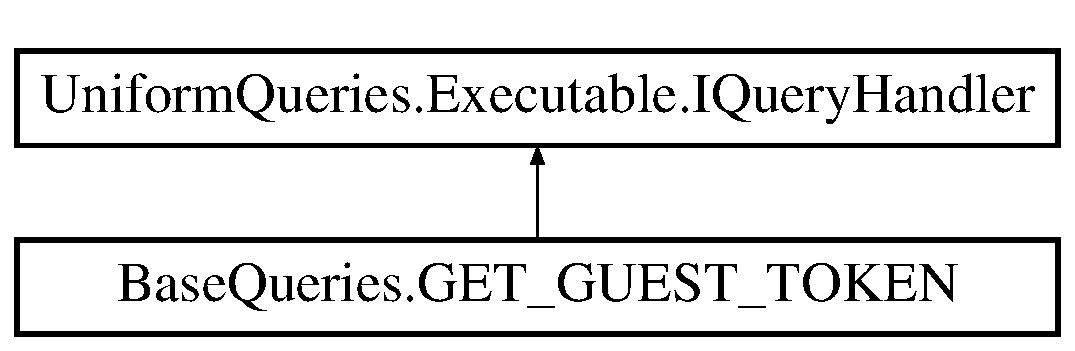
\includegraphics[height=2.000000cm]{d2/da1/class_base_queries_1_1_g_e_t___g_u_e_s_t___t_o_k_e_n}
\end{center}
\end{figure}
\subsection*{Classes}
\begin{DoxyCompactItemize}
\item 
class \mbox{\hyperlink{class_base_queries_1_1_g_e_t___g_u_e_s_t___t_o_k_e_n_1_1_guest_token_processor}{Guest\+Token\+Processor}}
\begin{DoxyCompactList}\small\item\em Handler that provide standartized way to recive guest token. \end{DoxyCompactList}\end{DoxyCompactItemize}
\subsection*{Public Member Functions}
\begin{DoxyCompactItemize}
\item 
\mbox{\Hypertarget{class_base_queries_1_1_g_e_t___g_u_e_s_t___t_o_k_e_n_a14602bc19c65ba7d11abf85e5e0f74a6}\label{class_base_queries_1_1_g_e_t___g_u_e_s_t___t_o_k_e_n_a14602bc19c65ba7d11abf85e5e0f74a6}} 
delegate string {\bfseries Guest\+Token\+Handler} ()
\item 
string \mbox{\hyperlink{class_base_queries_1_1_g_e_t___g_u_e_s_t___t_o_k_e_n_a06d62fabd5b44fb6b9975da1b72308a2}{Description}} (string culture\+Key)
\begin{DoxyCompactList}\small\item\em Return the description relative to the lenguage code or default if not found. \end{DoxyCompactList}\item 
void \mbox{\hyperlink{class_base_queries_1_1_g_e_t___g_u_e_s_t___t_o_k_e_n_afbad0ace27a743793bccea51a5c39db5}{Execute}} (\mbox{\hyperlink{struct_uniform_queries_1_1_query_part}{Query\+Part}}\mbox{[}$\,$\mbox{]} query\+Parts)
\begin{DoxyCompactList}\small\item\em Methods that process query. \end{DoxyCompactList}\item 
bool \mbox{\hyperlink{class_base_queries_1_1_g_e_t___g_u_e_s_t___t_o_k_e_n_adb9e113e010750eeedd261ce6811da1c}{Is\+Target}} (\mbox{\hyperlink{struct_uniform_queries_1_1_query_part}{Query\+Part}}\mbox{[}$\,$\mbox{]} query\+Parts)
\begin{DoxyCompactList}\small\item\em Check by the entry params does it target Query Handler. \end{DoxyCompactList}\end{DoxyCompactItemize}
\subsection*{Static Public Attributes}
\begin{DoxyCompactItemize}
\item 
static Guest\+Token\+Handler \mbox{\hyperlink{class_base_queries_1_1_g_e_t___g_u_e_s_t___t_o_k_e_n_abf7dded72bc2a686ab8e179a413efaae}{guest\+Token\+Handler}}
\begin{DoxyCompactList}\small\item\em Handler that would be userd to generating and authorizing of guest tokens. Return generated token in string format. \end{DoxyCompactList}\end{DoxyCompactItemize}


\subsection{Detailed Description}
Registrate token with guest rights in the system and return to client. 



\subsection{Member Function Documentation}
\mbox{\Hypertarget{class_base_queries_1_1_g_e_t___g_u_e_s_t___t_o_k_e_n_a06d62fabd5b44fb6b9975da1b72308a2}\label{class_base_queries_1_1_g_e_t___g_u_e_s_t___t_o_k_e_n_a06d62fabd5b44fb6b9975da1b72308a2}} 
\index{Base\+Queries\+::\+G\+E\+T\+\_\+\+G\+U\+E\+S\+T\+\_\+\+T\+O\+K\+EN@{Base\+Queries\+::\+G\+E\+T\+\_\+\+G\+U\+E\+S\+T\+\_\+\+T\+O\+K\+EN}!Description@{Description}}
\index{Description@{Description}!Base\+Queries\+::\+G\+E\+T\+\_\+\+G\+U\+E\+S\+T\+\_\+\+T\+O\+K\+EN@{Base\+Queries\+::\+G\+E\+T\+\_\+\+G\+U\+E\+S\+T\+\_\+\+T\+O\+K\+EN}}
\subsubsection{\texorpdfstring{Description()}{Description()}}
{\footnotesize\ttfamily string Base\+Queries.\+G\+E\+T\+\_\+\+G\+U\+E\+S\+T\+\_\+\+T\+O\+K\+E\+N.\+Description (\begin{DoxyParamCaption}\item[{string}]{culture\+Key }\end{DoxyParamCaption})}



Return the description relative to the lenguage code or default if not found. 


\begin{DoxyParams}{Parameters}
{\em culture\+Key} & \\
\hline
\end{DoxyParams}
\begin{DoxyReturn}{Returns}

\end{DoxyReturn}


Implements \mbox{\hyperlink{interface_uniform_queries_1_1_executable_1_1_i_query_handler_ae0e55919571d5456af31298394d241a9}{Uniform\+Queries.\+Executable.\+I\+Query\+Handler}}.

\mbox{\Hypertarget{class_base_queries_1_1_g_e_t___g_u_e_s_t___t_o_k_e_n_afbad0ace27a743793bccea51a5c39db5}\label{class_base_queries_1_1_g_e_t___g_u_e_s_t___t_o_k_e_n_afbad0ace27a743793bccea51a5c39db5}} 
\index{Base\+Queries\+::\+G\+E\+T\+\_\+\+G\+U\+E\+S\+T\+\_\+\+T\+O\+K\+EN@{Base\+Queries\+::\+G\+E\+T\+\_\+\+G\+U\+E\+S\+T\+\_\+\+T\+O\+K\+EN}!Execute@{Execute}}
\index{Execute@{Execute}!Base\+Queries\+::\+G\+E\+T\+\_\+\+G\+U\+E\+S\+T\+\_\+\+T\+O\+K\+EN@{Base\+Queries\+::\+G\+E\+T\+\_\+\+G\+U\+E\+S\+T\+\_\+\+T\+O\+K\+EN}}
\subsubsection{\texorpdfstring{Execute()}{Execute()}}
{\footnotesize\ttfamily void Base\+Queries.\+G\+E\+T\+\_\+\+G\+U\+E\+S\+T\+\_\+\+T\+O\+K\+E\+N.\+Execute (\begin{DoxyParamCaption}\item[{\mbox{\hyperlink{struct_uniform_queries_1_1_query_part}{Query\+Part}} \mbox{[}$\,$\mbox{]}}]{query\+Parts }\end{DoxyParamCaption})}



Methods that process query. 


\begin{DoxyParams}{Parameters}
{\em query\+Parts} & \\
\hline
\end{DoxyParams}


Implements \mbox{\hyperlink{interface_uniform_queries_1_1_executable_1_1_i_query_handler_a3268d72c0388f5e3debba4d73bdfe523}{Uniform\+Queries.\+Executable.\+I\+Query\+Handler}}.

\mbox{\Hypertarget{class_base_queries_1_1_g_e_t___g_u_e_s_t___t_o_k_e_n_adb9e113e010750eeedd261ce6811da1c}\label{class_base_queries_1_1_g_e_t___g_u_e_s_t___t_o_k_e_n_adb9e113e010750eeedd261ce6811da1c}} 
\index{Base\+Queries\+::\+G\+E\+T\+\_\+\+G\+U\+E\+S\+T\+\_\+\+T\+O\+K\+EN@{Base\+Queries\+::\+G\+E\+T\+\_\+\+G\+U\+E\+S\+T\+\_\+\+T\+O\+K\+EN}!Is\+Target@{Is\+Target}}
\index{Is\+Target@{Is\+Target}!Base\+Queries\+::\+G\+E\+T\+\_\+\+G\+U\+E\+S\+T\+\_\+\+T\+O\+K\+EN@{Base\+Queries\+::\+G\+E\+T\+\_\+\+G\+U\+E\+S\+T\+\_\+\+T\+O\+K\+EN}}
\subsubsection{\texorpdfstring{Is\+Target()}{IsTarget()}}
{\footnotesize\ttfamily bool Base\+Queries.\+G\+E\+T\+\_\+\+G\+U\+E\+S\+T\+\_\+\+T\+O\+K\+E\+N.\+Is\+Target (\begin{DoxyParamCaption}\item[{\mbox{\hyperlink{struct_uniform_queries_1_1_query_part}{Query\+Part}} \mbox{[}$\,$\mbox{]}}]{query\+Parts }\end{DoxyParamCaption})}



Check by the entry params does it target Query Handler. 


\begin{DoxyParams}{Parameters}
{\em query\+Parts} & \\
\hline
\end{DoxyParams}
\begin{DoxyReturn}{Returns}

\end{DoxyReturn}


Implements \mbox{\hyperlink{interface_uniform_queries_1_1_executable_1_1_i_query_handler_a0f43184bf3e306a7cbebc39098f044ee}{Uniform\+Queries.\+Executable.\+I\+Query\+Handler}}.



\subsection{Member Data Documentation}
\mbox{\Hypertarget{class_base_queries_1_1_g_e_t___g_u_e_s_t___t_o_k_e_n_abf7dded72bc2a686ab8e179a413efaae}\label{class_base_queries_1_1_g_e_t___g_u_e_s_t___t_o_k_e_n_abf7dded72bc2a686ab8e179a413efaae}} 
\index{Base\+Queries\+::\+G\+E\+T\+\_\+\+G\+U\+E\+S\+T\+\_\+\+T\+O\+K\+EN@{Base\+Queries\+::\+G\+E\+T\+\_\+\+G\+U\+E\+S\+T\+\_\+\+T\+O\+K\+EN}!guest\+Token\+Handler@{guest\+Token\+Handler}}
\index{guest\+Token\+Handler@{guest\+Token\+Handler}!Base\+Queries\+::\+G\+E\+T\+\_\+\+G\+U\+E\+S\+T\+\_\+\+T\+O\+K\+EN@{Base\+Queries\+::\+G\+E\+T\+\_\+\+G\+U\+E\+S\+T\+\_\+\+T\+O\+K\+EN}}
\subsubsection{\texorpdfstring{guest\+Token\+Handler}{guestTokenHandler}}
{\footnotesize\ttfamily Guest\+Token\+Handler Base\+Queries.\+G\+E\+T\+\_\+\+G\+U\+E\+S\+T\+\_\+\+T\+O\+K\+E\+N.\+guest\+Token\+Handler\hspace{0.3cm}{\ttfamily [static]}}



Handler that would be userd to generating and authorizing of guest tokens. Return generated token in string format. 



The documentation for this class was generated from the following file\+:\begin{DoxyCompactItemize}
\item 
D\+:/\+Work/\+Git\+Hub/doloro-\/networking-\/framework/\+Core/\+D\+N\+F\+Core/\+Base\+Queries/G\+E\+T\+\_\+\+G\+U\+E\+S\+T\+\_\+\+T\+O\+K\+E\+N.\+cs\end{DoxyCompactItemize}

\hypertarget{class_base_queries_1_1_g_e_t___p_u_b_l_i_c___k_e_y}{}\section{Base\+Queries.\+G\+E\+T\+\_\+\+P\+U\+B\+L\+I\+C\+\_\+\+K\+EY Class Reference}
\label{class_base_queries_1_1_g_e_t___p_u_b_l_i_c___k_e_y}\index{Base\+Queries.\+G\+E\+T\+\_\+\+P\+U\+B\+L\+I\+C\+\_\+\+K\+EY@{Base\+Queries.\+G\+E\+T\+\_\+\+P\+U\+B\+L\+I\+C\+\_\+\+K\+EY}}


Query that request from server public encription key (R\+SA algorithm).  


Inheritance diagram for Base\+Queries.\+G\+E\+T\+\_\+\+P\+U\+B\+L\+I\+C\+\_\+\+K\+EY\+:\begin{figure}[H]
\begin{center}
\leavevmode
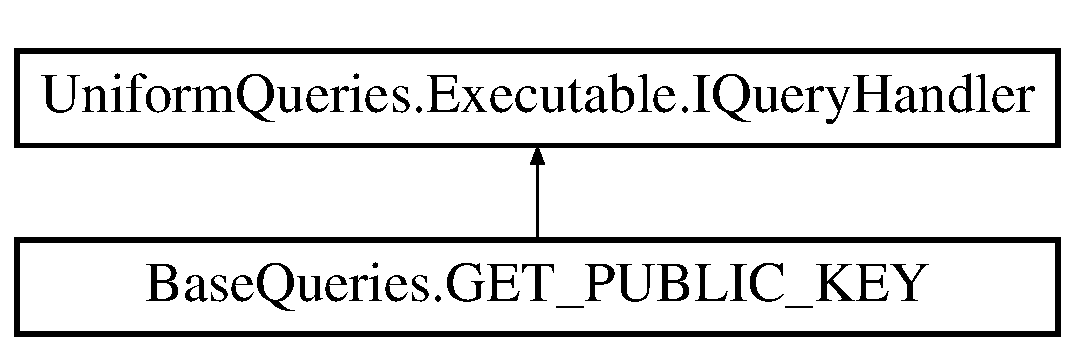
\includegraphics[height=2.000000cm]{da/d28/class_base_queries_1_1_g_e_t___p_u_b_l_i_c___k_e_y}
\end{center}
\end{figure}
\subsection*{Public Member Functions}
\begin{DoxyCompactItemize}
\item 
string \mbox{\hyperlink{class_base_queries_1_1_g_e_t___p_u_b_l_i_c___k_e_y_afcd94e8596f6c015a1a60c987d53cfa8}{Description}} (string culture\+Key)
\begin{DoxyCompactList}\small\item\em Return the description relative to the lenguage code or default if not found. \end{DoxyCompactList}\item 
void \mbox{\hyperlink{class_base_queries_1_1_g_e_t___p_u_b_l_i_c___k_e_y_a6351a2ced538508e861a1829864d1d0d}{Execute}} (\mbox{\hyperlink{struct_uniform_queries_1_1_query_part}{Query\+Part}}\mbox{[}$\,$\mbox{]} query\+Parts)
\begin{DoxyCompactList}\small\item\em Methods that process query. \end{DoxyCompactList}\item 
bool \mbox{\hyperlink{class_base_queries_1_1_g_e_t___p_u_b_l_i_c___k_e_y_a15316117d19cd8d85fb90a37bad5e9d7}{Is\+Target}} (\mbox{\hyperlink{struct_uniform_queries_1_1_query_part}{Query\+Part}}\mbox{[}$\,$\mbox{]} query\+Parts)
\begin{DoxyCompactList}\small\item\em Check by the entry params does it target Query Handler. \end{DoxyCompactList}\end{DoxyCompactItemize}


\subsection{Detailed Description}
Query that request from server public encription key (R\+SA algorithm). 



\subsection{Member Function Documentation}
\mbox{\Hypertarget{class_base_queries_1_1_g_e_t___p_u_b_l_i_c___k_e_y_afcd94e8596f6c015a1a60c987d53cfa8}\label{class_base_queries_1_1_g_e_t___p_u_b_l_i_c___k_e_y_afcd94e8596f6c015a1a60c987d53cfa8}} 
\index{Base\+Queries\+::\+G\+E\+T\+\_\+\+P\+U\+B\+L\+I\+C\+\_\+\+K\+EY@{Base\+Queries\+::\+G\+E\+T\+\_\+\+P\+U\+B\+L\+I\+C\+\_\+\+K\+EY}!Description@{Description}}
\index{Description@{Description}!Base\+Queries\+::\+G\+E\+T\+\_\+\+P\+U\+B\+L\+I\+C\+\_\+\+K\+EY@{Base\+Queries\+::\+G\+E\+T\+\_\+\+P\+U\+B\+L\+I\+C\+\_\+\+K\+EY}}
\subsubsection{\texorpdfstring{Description()}{Description()}}
{\footnotesize\ttfamily string Base\+Queries.\+G\+E\+T\+\_\+\+P\+U\+B\+L\+I\+C\+\_\+\+K\+E\+Y.\+Description (\begin{DoxyParamCaption}\item[{string}]{culture\+Key }\end{DoxyParamCaption})}



Return the description relative to the lenguage code or default if not found. 


\begin{DoxyParams}{Parameters}
{\em culture\+Key} & \\
\hline
\end{DoxyParams}
\begin{DoxyReturn}{Returns}

\end{DoxyReturn}


Implements \mbox{\hyperlink{interface_uniform_queries_1_1_executable_1_1_i_query_handler_ae0e55919571d5456af31298394d241a9}{Uniform\+Queries.\+Executable.\+I\+Query\+Handler}}.

\mbox{\Hypertarget{class_base_queries_1_1_g_e_t___p_u_b_l_i_c___k_e_y_a6351a2ced538508e861a1829864d1d0d}\label{class_base_queries_1_1_g_e_t___p_u_b_l_i_c___k_e_y_a6351a2ced538508e861a1829864d1d0d}} 
\index{Base\+Queries\+::\+G\+E\+T\+\_\+\+P\+U\+B\+L\+I\+C\+\_\+\+K\+EY@{Base\+Queries\+::\+G\+E\+T\+\_\+\+P\+U\+B\+L\+I\+C\+\_\+\+K\+EY}!Execute@{Execute}}
\index{Execute@{Execute}!Base\+Queries\+::\+G\+E\+T\+\_\+\+P\+U\+B\+L\+I\+C\+\_\+\+K\+EY@{Base\+Queries\+::\+G\+E\+T\+\_\+\+P\+U\+B\+L\+I\+C\+\_\+\+K\+EY}}
\subsubsection{\texorpdfstring{Execute()}{Execute()}}
{\footnotesize\ttfamily void Base\+Queries.\+G\+E\+T\+\_\+\+P\+U\+B\+L\+I\+C\+\_\+\+K\+E\+Y.\+Execute (\begin{DoxyParamCaption}\item[{\mbox{\hyperlink{struct_uniform_queries_1_1_query_part}{Query\+Part}} \mbox{[}$\,$\mbox{]}}]{query\+Parts }\end{DoxyParamCaption})}



Methods that process query. 


\begin{DoxyParams}{Parameters}
{\em query\+Parts} & \\
\hline
\end{DoxyParams}


Implements \mbox{\hyperlink{interface_uniform_queries_1_1_executable_1_1_i_query_handler_a3268d72c0388f5e3debba4d73bdfe523}{Uniform\+Queries.\+Executable.\+I\+Query\+Handler}}.

\mbox{\Hypertarget{class_base_queries_1_1_g_e_t___p_u_b_l_i_c___k_e_y_a15316117d19cd8d85fb90a37bad5e9d7}\label{class_base_queries_1_1_g_e_t___p_u_b_l_i_c___k_e_y_a15316117d19cd8d85fb90a37bad5e9d7}} 
\index{Base\+Queries\+::\+G\+E\+T\+\_\+\+P\+U\+B\+L\+I\+C\+\_\+\+K\+EY@{Base\+Queries\+::\+G\+E\+T\+\_\+\+P\+U\+B\+L\+I\+C\+\_\+\+K\+EY}!Is\+Target@{Is\+Target}}
\index{Is\+Target@{Is\+Target}!Base\+Queries\+::\+G\+E\+T\+\_\+\+P\+U\+B\+L\+I\+C\+\_\+\+K\+EY@{Base\+Queries\+::\+G\+E\+T\+\_\+\+P\+U\+B\+L\+I\+C\+\_\+\+K\+EY}}
\subsubsection{\texorpdfstring{Is\+Target()}{IsTarget()}}
{\footnotesize\ttfamily bool Base\+Queries.\+G\+E\+T\+\_\+\+P\+U\+B\+L\+I\+C\+\_\+\+K\+E\+Y.\+Is\+Target (\begin{DoxyParamCaption}\item[{\mbox{\hyperlink{struct_uniform_queries_1_1_query_part}{Query\+Part}} \mbox{[}$\,$\mbox{]}}]{query\+Parts }\end{DoxyParamCaption})}



Check by the entry params does it target Query Handler. 


\begin{DoxyParams}{Parameters}
{\em query\+Parts} & \\
\hline
\end{DoxyParams}
\begin{DoxyReturn}{Returns}

\end{DoxyReturn}


Implements \mbox{\hyperlink{interface_uniform_queries_1_1_executable_1_1_i_query_handler_a0f43184bf3e306a7cbebc39098f044ee}{Uniform\+Queries.\+Executable.\+I\+Query\+Handler}}.



The documentation for this class was generated from the following file\+:\begin{DoxyCompactItemize}
\item 
D\+:/\+Work/\+Git\+Hub/doloro-\/networking-\/framework/\+Core/\+D\+N\+F\+Core/\+Base\+Queries/G\+E\+T\+\_\+\+P\+U\+B\+L\+I\+C\+\_\+\+K\+E\+Y.\+cs\end{DoxyCompactItemize}

\hypertarget{class_base_queries_1_1_g_e_t___g_u_e_s_t___t_o_k_e_n_1_1_guest_token_processor}{}\section{Base\+Queries.\+G\+E\+T\+\_\+\+G\+U\+E\+S\+T\+\_\+\+T\+O\+K\+E\+N.\+Guest\+Token\+Processor Class Reference}
\label{class_base_queries_1_1_g_e_t___g_u_e_s_t___t_o_k_e_n_1_1_guest_token_processor}\index{Base\+Queries.\+G\+E\+T\+\_\+\+G\+U\+E\+S\+T\+\_\+\+T\+O\+K\+E\+N.\+Guest\+Token\+Processor@{Base\+Queries.\+G\+E\+T\+\_\+\+G\+U\+E\+S\+T\+\_\+\+T\+O\+K\+E\+N.\+Guest\+Token\+Processor}}


Handler that provide standartized way to recive guest token.  


Inheritance diagram for Base\+Queries.\+G\+E\+T\+\_\+\+G\+U\+E\+S\+T\+\_\+\+T\+O\+K\+E\+N.\+Guest\+Token\+Processor\+:\begin{figure}[H]
\begin{center}
\leavevmode
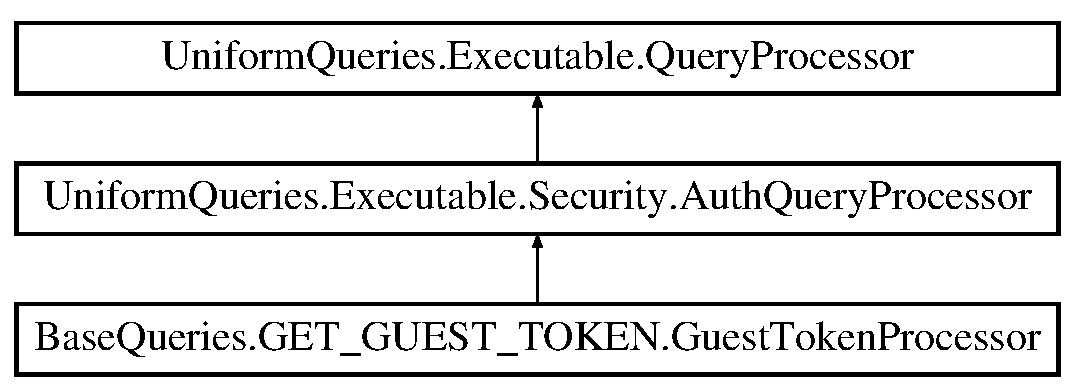
\includegraphics[height=3.000000cm]{d7/d42/class_base_queries_1_1_g_e_t___g_u_e_s_t___t_o_k_e_n_1_1_guest_token_processor}
\end{center}
\end{figure}
\subsection*{Public Member Functions}
\begin{DoxyCompactItemize}
\item 
\mbox{\Hypertarget{class_base_queries_1_1_g_e_t___g_u_e_s_t___t_o_k_e_n_1_1_guest_token_processor_af9d9d6f5a3ca70f467099d6b8dac438b}\label{class_base_queries_1_1_g_e_t___g_u_e_s_t___t_o_k_e_n_1_1_guest_token_processor_af9d9d6f5a3ca70f467099d6b8dac438b}} 
async void {\bfseries Try\+To\+Recive\+Token\+Async} (string server\+IP, string pipe\+Name, Cancellation\+Token cancellation\+Token)
\end{DoxyCompactItemize}
\subsection*{Additional Inherited Members}


\subsection{Detailed Description}
Handler that provide standartized way to recive guest token. 



The documentation for this class was generated from the following file\+:\begin{DoxyCompactItemize}
\item 
D\+:/\+Work/\+Git\+Hub/doloro-\/networking-\/framework/\+Core/\+D\+N\+F\+Core/\+Base\+Queries/G\+E\+T\+\_\+\+G\+U\+E\+S\+T\+\_\+\+T\+O\+K\+E\+N.\+cs\end{DoxyCompactItemize}

\hypertarget{class_authority_controller_1_1_data_1_1_handler}{}\section{Authority\+Controller.\+Data.\+Handler Class Reference}
\label{class_authority_controller_1_1_data_1_1_handler}\index{Authority\+Controller.\+Data.\+Handler@{Authority\+Controller.\+Data.\+Handler}}


Provide metods that simplifying work with data.  


\subsection*{Static Public Member Functions}
\begin{DoxyCompactItemize}
\item 
static bool \mbox{\hyperlink{class_authority_controller_1_1_data_1_1_handler_a7f4e5dd2a2f300e566116810897e7f2f}{Try\+X\+M\+L\+Serialize$<$ T $>$}} (T data, out string xml)
\begin{DoxyCompactList}\small\item\em Trying to serialize obkject to X\+ML format. \end{DoxyCompactList}\item 
static bool \mbox{\hyperlink{class_authority_controller_1_1_data_1_1_handler_a086874112fede63b9d3bb8c070698c55}{Try\+X\+M\+L\+Deserizlize$<$ T $>$}} (string xml, out T data)
\begin{DoxyCompactList}\small\item\em Trying to convert X\+ML string to object instance. \end{DoxyCompactList}\item 
static void \mbox{\hyperlink{class_authority_controller_1_1_data_1_1_handler_ae44331f9a2598461455b9f478992e71c}{Save\+As$<$ T $>$}} (object obj, string directory, string file\+Name)
\begin{DoxyCompactList}\small\item\em Saving config file to directory. \end{DoxyCompactList}\item 
static bool \mbox{\hyperlink{class_authority_controller_1_1_data_1_1_handler_aad3bc4d6c6017f4061261f15935da6dc}{Try\+To\+Load$<$ T $>$}} (string path, out T result)
\begin{DoxyCompactList}\small\item\em Trying to deserialize object from X\+ML file. \end{DoxyCompactList}\end{DoxyCompactItemize}


\subsection{Detailed Description}
Provide metods that simplifying work with data. 



\subsection{Member Function Documentation}
\mbox{\Hypertarget{class_authority_controller_1_1_data_1_1_handler_ae44331f9a2598461455b9f478992e71c}\label{class_authority_controller_1_1_data_1_1_handler_ae44331f9a2598461455b9f478992e71c}} 
\index{Authority\+Controller\+::\+Data\+::\+Handler@{Authority\+Controller\+::\+Data\+::\+Handler}!Save\+As$<$ T $>$@{Save\+As$<$ T $>$}}
\index{Save\+As$<$ T $>$@{Save\+As$<$ T $>$}!Authority\+Controller\+::\+Data\+::\+Handler@{Authority\+Controller\+::\+Data\+::\+Handler}}
\subsubsection{\texorpdfstring{Save\+As$<$ T $>$()}{SaveAs< T >()}}
{\footnotesize\ttfamily static void Authority\+Controller.\+Data.\+Handler.\+Save\+As$<$ T $>$ (\begin{DoxyParamCaption}\item[{object}]{obj,  }\item[{string}]{directory,  }\item[{string}]{file\+Name }\end{DoxyParamCaption})\hspace{0.3cm}{\ttfamily [static]}}



Saving config file to directory. 


\begin{DoxyParams}{Parameters}
{\em directory} & \\
\hline
{\em file\+Name} & \\
\hline
\end{DoxyParams}
\mbox{\Hypertarget{class_authority_controller_1_1_data_1_1_handler_aad3bc4d6c6017f4061261f15935da6dc}\label{class_authority_controller_1_1_data_1_1_handler_aad3bc4d6c6017f4061261f15935da6dc}} 
\index{Authority\+Controller\+::\+Data\+::\+Handler@{Authority\+Controller\+::\+Data\+::\+Handler}!Try\+To\+Load$<$ T $>$@{Try\+To\+Load$<$ T $>$}}
\index{Try\+To\+Load$<$ T $>$@{Try\+To\+Load$<$ T $>$}!Authority\+Controller\+::\+Data\+::\+Handler@{Authority\+Controller\+::\+Data\+::\+Handler}}
\subsubsection{\texorpdfstring{Try\+To\+Load$<$ T $>$()}{TryToLoad< T >()}}
{\footnotesize\ttfamily static bool Authority\+Controller.\+Data.\+Handler.\+Try\+To\+Load$<$ T $>$ (\begin{DoxyParamCaption}\item[{string}]{path,  }\item[{out T}]{result }\end{DoxyParamCaption})\hspace{0.3cm}{\ttfamily [static]}}



Trying to deserialize object from X\+ML file. 


\begin{DoxyTemplParams}{Template Parameters}
{\em T} & Required type\\
\hline
\end{DoxyTemplParams}

\begin{DoxyParams}{Parameters}
{\em path} & Full path to file.\\
\hline
{\em result} & Deserizlised object.\\
\hline
\end{DoxyParams}
\begin{DoxyReturn}{Returns}

\end{DoxyReturn}
\mbox{\Hypertarget{class_authority_controller_1_1_data_1_1_handler_a086874112fede63b9d3bb8c070698c55}\label{class_authority_controller_1_1_data_1_1_handler_a086874112fede63b9d3bb8c070698c55}} 
\index{Authority\+Controller\+::\+Data\+::\+Handler@{Authority\+Controller\+::\+Data\+::\+Handler}!Try\+X\+M\+L\+Deserizlize$<$ T $>$@{Try\+X\+M\+L\+Deserizlize$<$ T $>$}}
\index{Try\+X\+M\+L\+Deserizlize$<$ T $>$@{Try\+X\+M\+L\+Deserizlize$<$ T $>$}!Authority\+Controller\+::\+Data\+::\+Handler@{Authority\+Controller\+::\+Data\+::\+Handler}}
\subsubsection{\texorpdfstring{Try\+X\+M\+L\+Deserizlize$<$ T $>$()}{TryXMLDeserizlize< T >()}}
{\footnotesize\ttfamily static bool Authority\+Controller.\+Data.\+Handler.\+Try\+X\+M\+L\+Deserizlize$<$ T $>$ (\begin{DoxyParamCaption}\item[{string}]{xml,  }\item[{out T}]{data }\end{DoxyParamCaption})\hspace{0.3cm}{\ttfamily [static]}}



Trying to convert X\+ML string to object instance. 


\begin{DoxyParams}{Parameters}
{\em xml} & X\+ML string format of object.\\
\hline
{\em data} & Instiniated object.\\
\hline
\end{DoxyParams}
\begin{DoxyReturn}{Returns}
Does convertation passed success.
\end{DoxyReturn}
\mbox{\Hypertarget{class_authority_controller_1_1_data_1_1_handler_a7f4e5dd2a2f300e566116810897e7f2f}\label{class_authority_controller_1_1_data_1_1_handler_a7f4e5dd2a2f300e566116810897e7f2f}} 
\index{Authority\+Controller\+::\+Data\+::\+Handler@{Authority\+Controller\+::\+Data\+::\+Handler}!Try\+X\+M\+L\+Serialize$<$ T $>$@{Try\+X\+M\+L\+Serialize$<$ T $>$}}
\index{Try\+X\+M\+L\+Serialize$<$ T $>$@{Try\+X\+M\+L\+Serialize$<$ T $>$}!Authority\+Controller\+::\+Data\+::\+Handler@{Authority\+Controller\+::\+Data\+::\+Handler}}
\subsubsection{\texorpdfstring{Try\+X\+M\+L\+Serialize$<$ T $>$()}{TryXMLSerialize< T >()}}
{\footnotesize\ttfamily static bool Authority\+Controller.\+Data.\+Handler.\+Try\+X\+M\+L\+Serialize$<$ T $>$ (\begin{DoxyParamCaption}\item[{T}]{data,  }\item[{out string}]{xml }\end{DoxyParamCaption})\hspace{0.3cm}{\ttfamily [static]}}



Trying to serialize obkject to X\+ML format. 


\begin{DoxyParams}{Parameters}
{\em data} & Object to serizlization.\\
\hline
{\em xml} & Object in string format.\\
\hline
\end{DoxyParams}
\begin{DoxyReturn}{Returns}

\end{DoxyReturn}


The documentation for this class was generated from the following file\+:\begin{DoxyCompactItemize}
\item 
D\+:/\+Work/\+Git\+Hub/doloro-\/networking-\/framework/\+Addons/\+Authority\+Controller/\+Data/Handler.\+cs\end{DoxyCompactItemize}

\hypertarget{class_pipes_provider_1_1_networking_1_1_info}{}\section{Pipes\+Provider.\+Networking.\+Info Class Reference}
\label{class_pipes_provider_1_1_networking_1_1_info}\index{Pipes\+Provider.\+Networking.\+Info@{Pipes\+Provider.\+Networking.\+Info}}


Class that provide A\+PI for network information.  


\subsection*{Static Public Member Functions}
\begin{DoxyCompactItemize}
\item 
static void \mbox{\hyperlink{class_pipes_provider_1_1_networking_1_1_info_af2fa3a471e2f6245bed859c86b6f0c0e}{Try\+Get\+Host\+Name}} (string ip\+Address, ref string output)
\begin{DoxyCompactList}\small\item\em Conver ip adress of server to host name. \end{DoxyCompactList}\item 
static async void \mbox{\hyperlink{class_pipes_provider_1_1_networking_1_1_info_aa609196312941e05536dcb3526b9a2ce}{Ping\+Host}} (string host\+Uri, int port\+Number, System.\+Action$<$ string, int $>$ callback)
\begin{DoxyCompactList}\small\item\em Ping server by U\+RI via requested port. In case if cooecntion established will call callback where\+: \end{DoxyCompactList}\item 
\mbox{\Hypertarget{class_pipes_provider_1_1_networking_1_1_info_a3bc757d31da1bf0759a252ee0f919917}\label{class_pipes_provider_1_1_networking_1_1_info_a3bc757d31da1bf0759a252ee0f919917}} 
static string \mbox{[}$\,$\mbox{]} {\bfseries Server\+Name} ()
\item 
static string \mbox{[}$\,$\mbox{]} \mbox{\hyperlink{class_pipes_provider_1_1_networking_1_1_info_ac8097e6a6bccbeae15e309ce72dbac91}{Display\+I\+P\+Addresses}} ()
\begin{DoxyCompactList}\small\item\em Provide IP addresses for every relevant network interface. \end{DoxyCompactList}\end{DoxyCompactItemize}


\subsection{Detailed Description}
Class that provide A\+PI for network information. 



\subsection{Member Function Documentation}
\mbox{\Hypertarget{class_pipes_provider_1_1_networking_1_1_info_ac8097e6a6bccbeae15e309ce72dbac91}\label{class_pipes_provider_1_1_networking_1_1_info_ac8097e6a6bccbeae15e309ce72dbac91}} 
\index{Pipes\+Provider\+::\+Networking\+::\+Info@{Pipes\+Provider\+::\+Networking\+::\+Info}!Display\+I\+P\+Addresses@{Display\+I\+P\+Addresses}}
\index{Display\+I\+P\+Addresses@{Display\+I\+P\+Addresses}!Pipes\+Provider\+::\+Networking\+::\+Info@{Pipes\+Provider\+::\+Networking\+::\+Info}}
\subsubsection{\texorpdfstring{Display\+I\+P\+Addresses()}{DisplayIPAddresses()}}
{\footnotesize\ttfamily static string \mbox{[}$\,$\mbox{]} Pipes\+Provider.\+Networking.\+Info.\+Display\+I\+P\+Addresses (\begin{DoxyParamCaption}{ }\end{DoxyParamCaption})\hspace{0.3cm}{\ttfamily [static]}}



Provide IP addresses for every relevant network interface. 

\begin{DoxyReturn}{Returns}

\end{DoxyReturn}
\mbox{\Hypertarget{class_pipes_provider_1_1_networking_1_1_info_aa609196312941e05536dcb3526b9a2ce}\label{class_pipes_provider_1_1_networking_1_1_info_aa609196312941e05536dcb3526b9a2ce}} 
\index{Pipes\+Provider\+::\+Networking\+::\+Info@{Pipes\+Provider\+::\+Networking\+::\+Info}!Ping\+Host@{Ping\+Host}}
\index{Ping\+Host@{Ping\+Host}!Pipes\+Provider\+::\+Networking\+::\+Info@{Pipes\+Provider\+::\+Networking\+::\+Info}}
\subsubsection{\texorpdfstring{Ping\+Host()}{PingHost()}}
{\footnotesize\ttfamily static async void Pipes\+Provider.\+Networking.\+Info.\+Ping\+Host (\begin{DoxyParamCaption}\item[{string}]{host\+Uri,  }\item[{int}]{port\+Number,  }\item[{System.\+Action$<$ string, int $>$}]{callback }\end{DoxyParamCaption})\hspace{0.3cm}{\ttfamily [static]}}



Ping server by U\+RI via requested port. In case if cooecntion established will call callback where\+: 


\begin{DoxyParams}{Parameters}
{\em host\+Uri} & \mbox{\hyperlink{namespace_pipes_provider_1_1_server}{Server}} uri.\\
\hline
{\em port\+Number} & Port for connection. Must be oppend.\\
\hline
{\em callback} & Method that will be called as callback when cooection will be established. string\+: uri int\+: port\\
\hline
\end{DoxyParams}
\mbox{\Hypertarget{class_pipes_provider_1_1_networking_1_1_info_af2fa3a471e2f6245bed859c86b6f0c0e}\label{class_pipes_provider_1_1_networking_1_1_info_af2fa3a471e2f6245bed859c86b6f0c0e}} 
\index{Pipes\+Provider\+::\+Networking\+::\+Info@{Pipes\+Provider\+::\+Networking\+::\+Info}!Try\+Get\+Host\+Name@{Try\+Get\+Host\+Name}}
\index{Try\+Get\+Host\+Name@{Try\+Get\+Host\+Name}!Pipes\+Provider\+::\+Networking\+::\+Info@{Pipes\+Provider\+::\+Networking\+::\+Info}}
\subsubsection{\texorpdfstring{Try\+Get\+Host\+Name()}{TryGetHostName()}}
{\footnotesize\ttfamily static void Pipes\+Provider.\+Networking.\+Info.\+Try\+Get\+Host\+Name (\begin{DoxyParamCaption}\item[{string}]{ip\+Address,  }\item[{ref string}]{output }\end{DoxyParamCaption})\hspace{0.3cm}{\ttfamily [static]}}



Conver ip adress of server to host name. 


\begin{DoxyParams}{Parameters}
{\em ip\+Address} & \\
\hline
\end{DoxyParams}
\begin{DoxyReturn}{Returns}

\end{DoxyReturn}


The documentation for this class was generated from the following file\+:\begin{DoxyCompactItemize}
\item 
D\+:/\+Work/\+Git\+Hub/doloro-\/networking-\/framework/\+Pipes\+Provider/\+Networking/Info.\+cs\end{DoxyCompactItemize}

\hypertarget{class_pipes_provider_1_1_networking_1_1_routing_1_1_instruction}{}\section{Pipes\+Provider.\+Networking.\+Routing.\+Instruction Class Reference}
\label{class_pipes_provider_1_1_networking_1_1_routing_1_1_instruction}\index{Pipes\+Provider.\+Networking.\+Routing.\+Instruction@{Pipes\+Provider.\+Networking.\+Routing.\+Instruction}}


 


Inheritance diagram for Pipes\+Provider.\+Networking.\+Routing.\+Instruction\+:\begin{figure}[H]
\begin{center}
\leavevmode
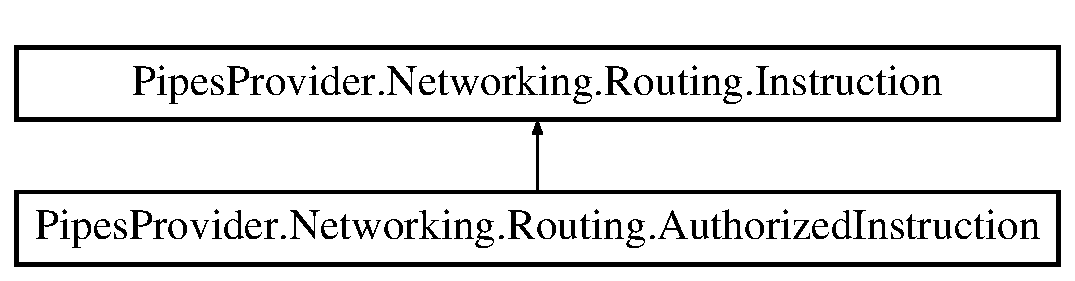
\includegraphics[height=2.000000cm]{d5/d2e/class_pipes_provider_1_1_networking_1_1_routing_1_1_instruction}
\end{center}
\end{figure}
\subsection*{Public Member Functions}
\begin{DoxyCompactItemize}
\item 
bool \mbox{\hyperlink{class_pipes_provider_1_1_networking_1_1_routing_1_1_instruction_a376135eac06c59b1df8d2f5d1617bed9}{Is\+Routing\+Target}} (string recived\+Query)
\begin{DoxyCompactList}\small\item\em Check doest this query must be routed using this server instruction. \end{DoxyCompactList}\item 
bool \mbox{\hyperlink{class_pipes_provider_1_1_networking_1_1_routing_1_1_instruction_a04ee08d3b41785e88679c6870c392266}{Try\+Update\+Public\+Key}} (object recived\+Query)
\begin{DoxyCompactList}\small\item\em Try to update Public R\+SA key by query recived from server as reply to G\+ET P\+U\+B\+L\+I\+C\+K\+EY query. \end{DoxyCompactList}\end{DoxyCompactItemize}
\subsection*{Public Attributes}
\begin{DoxyCompactItemize}
\item 
string \mbox{\hyperlink{class_pipes_provider_1_1_networking_1_1_routing_1_1_instruction_adb75f80ff34fab644305856ccf23d07b}{routing\+IP}} = \char`\"{}localhost\char`\"{}
\begin{DoxyCompactList}\small\item\em Address that will be ised for routing \end{DoxyCompactList}\item 
string \mbox{\hyperlink{class_pipes_provider_1_1_networking_1_1_routing_1_1_instruction_abe54e245df8dd26547b0c881b987202b}{pipe\+Name}} = \char`\"{}\char`\"{}
\begin{DoxyCompactList}\small\item\em neme of the named pipe for server access. \end{DoxyCompactList}\item 
\mbox{\hyperlink{struct_pipes_provider_1_1_security_1_1_logon_config}{Security.\+Logon\+Config}} \mbox{\hyperlink{class_pipes_provider_1_1_networking_1_1_routing_1_1_instruction_a2a3325abd7537b7a961626272634e038}{logon\+Config}} = \mbox{\hyperlink{struct_pipes_provider_1_1_security_1_1_logon_config_ad09f6e3c892826dc5df995e02f7a5738}{Security.\+Logon\+Config.\+Anonymous}}
\begin{DoxyCompactList}\small\item\em Logon config recuired to server connection. \end{DoxyCompactList}\item 
string \mbox{[}$\,$\mbox{]} \mbox{\hyperlink{class_pipes_provider_1_1_networking_1_1_routing_1_1_instruction_aa98823848a42831095f92b639121cc67}{query\+Patterns}} = new string\mbox{[}$\,$\mbox{]} \{ \char`\"{}\char`\"{} \}
\begin{DoxyCompactList}\small\item\em Array that contain querie\textquotesingle{}s body that need to be routed by this instruction. \end{DoxyCompactList}\item 
bool \mbox{\hyperlink{class_pipes_provider_1_1_networking_1_1_routing_1_1_instruction_a61ce6ffa8bb9cc44efc57bc51be3550b}{R\+S\+A\+Encryption}} = true
\begin{DoxyCompactList}\small\item\em Does this chanel has R\+SA encryption? If true then client can ask for server\textquotesingle{}s Public Key and encrypt message before send. \end{DoxyCompactList}\end{DoxyCompactItemize}
\subsection*{Properties}
\begin{DoxyCompactItemize}
\item 
R\+S\+A\+Parameters \mbox{\hyperlink{class_pipes_provider_1_1_networking_1_1_routing_1_1_instruction_a8681a89ae14ad25d11ee0c588231b772}{Public\+Key}}\hspace{0.3cm}{\ttfamily  \mbox{[}get, private set\mbox{]}}
\begin{DoxyCompactList}\small\item\em R\+SA public key that was recived from this server. \end{DoxyCompactList}\item 
Date\+Time \mbox{\hyperlink{class_pipes_provider_1_1_networking_1_1_routing_1_1_instruction_a60281a347236a1311c37743b90596d58}{Public\+Key\+Expire\+Time}}\hspace{0.3cm}{\ttfamily  \mbox{[}get, private set\mbox{]}}
\begin{DoxyCompactList}\small\item\em Time when public key will become expired. \end{DoxyCompactList}\item 
bool \mbox{\hyperlink{class_pipes_provider_1_1_networking_1_1_routing_1_1_instruction_a07dbb5b97b3d9a28e5a318815d954278}{Is\+Valid}}\hspace{0.3cm}{\ttfamily  \mbox{[}get, private set\mbox{]}}
\begin{DoxyCompactList}\small\item\em Check does loading was failed or key was expired. \end{DoxyCompactList}\item 
static \mbox{\hyperlink{class_pipes_provider_1_1_networking_1_1_routing_1_1_instruction}{Instruction}} \mbox{\hyperlink{class_pipes_provider_1_1_networking_1_1_routing_1_1_instruction_a7b1790dc22b0fd1a11b447e207245e83}{Default}}\hspace{0.3cm}{\ttfamily  \mbox{[}get\mbox{]}}
\begin{DoxyCompactList}\small\item\em Return default instruction. \end{DoxyCompactList}\item 
static \mbox{\hyperlink{class_pipes_provider_1_1_networking_1_1_routing_1_1_instruction}{Instruction}} \mbox{\hyperlink{class_pipes_provider_1_1_networking_1_1_routing_1_1_instruction_aad2d50b60ddcdd0c7d0671ced01a5480}{Empty}}\hspace{0.3cm}{\ttfamily  \mbox{[}get\mbox{]}}
\begin{DoxyCompactList}\small\item\em Return empty instruction. \end{DoxyCompactList}\end{DoxyCompactItemize}
\subsection*{Private Attributes}
\begin{DoxyCompactItemize}
\item 
\mbox{\Hypertarget{class_pipes_provider_1_1_networking_1_1_routing_1_1_instruction_abcd8b85ff0383ecd73b24befa9d69506}\label{class_pipes_provider_1_1_networking_1_1_routing_1_1_instruction_abcd8b85ff0383ecd73b24befa9d69506}} 
bool {\bfseries \+\_\+is\+Valid} = true
\end{DoxyCompactItemize}


\subsection{Detailed Description}


Struct that contain instruction about target adress by relative query params. Allow using of several servers via one public.

Example\+: $<$--$>$ Authification server \mbox{\hyperlink{namespace_pipes_provider_1_1_client}{Client}} $<$--$>$ Query server $<$--$>$ Data server 1 $<$--$>$ Data server 2 

\subsection{Member Function Documentation}
\mbox{\Hypertarget{class_pipes_provider_1_1_networking_1_1_routing_1_1_instruction_a376135eac06c59b1df8d2f5d1617bed9}\label{class_pipes_provider_1_1_networking_1_1_routing_1_1_instruction_a376135eac06c59b1df8d2f5d1617bed9}} 
\index{Pipes\+Provider\+::\+Networking\+::\+Routing\+::\+Instruction@{Pipes\+Provider\+::\+Networking\+::\+Routing\+::\+Instruction}!Is\+Routing\+Target@{Is\+Routing\+Target}}
\index{Is\+Routing\+Target@{Is\+Routing\+Target}!Pipes\+Provider\+::\+Networking\+::\+Routing\+::\+Instruction@{Pipes\+Provider\+::\+Networking\+::\+Routing\+::\+Instruction}}
\subsubsection{\texorpdfstring{Is\+Routing\+Target()}{IsRoutingTarget()}}
{\footnotesize\ttfamily bool Pipes\+Provider.\+Networking.\+Routing.\+Instruction.\+Is\+Routing\+Target (\begin{DoxyParamCaption}\item[{string}]{recived\+Query }\end{DoxyParamCaption})}



Check doest this query must be routed using this server instruction. 


\begin{DoxyParams}{Parameters}
{\em recived\+Query} & \\
\hline
\end{DoxyParams}
\begin{DoxyReturn}{Returns}

\end{DoxyReturn}
\mbox{\Hypertarget{class_pipes_provider_1_1_networking_1_1_routing_1_1_instruction_a04ee08d3b41785e88679c6870c392266}\label{class_pipes_provider_1_1_networking_1_1_routing_1_1_instruction_a04ee08d3b41785e88679c6870c392266}} 
\index{Pipes\+Provider\+::\+Networking\+::\+Routing\+::\+Instruction@{Pipes\+Provider\+::\+Networking\+::\+Routing\+::\+Instruction}!Try\+Update\+Public\+Key@{Try\+Update\+Public\+Key}}
\index{Try\+Update\+Public\+Key@{Try\+Update\+Public\+Key}!Pipes\+Provider\+::\+Networking\+::\+Routing\+::\+Instruction@{Pipes\+Provider\+::\+Networking\+::\+Routing\+::\+Instruction}}
\subsubsection{\texorpdfstring{Try\+Update\+Public\+Key()}{TryUpdatePublicKey()}}
{\footnotesize\ttfamily bool Pipes\+Provider.\+Networking.\+Routing.\+Instruction.\+Try\+Update\+Public\+Key (\begin{DoxyParamCaption}\item[{object}]{recived\+Query }\end{DoxyParamCaption})}



Try to update Public R\+SA key by query recived from server as reply to G\+ET P\+U\+B\+L\+I\+C\+K\+EY query. 


\begin{DoxyParams}{Parameters}
{\em recived\+Query} & \\
\hline
\end{DoxyParams}
\begin{DoxyReturn}{Returns}

\end{DoxyReturn}


\subsection{Member Data Documentation}
\mbox{\Hypertarget{class_pipes_provider_1_1_networking_1_1_routing_1_1_instruction_a2a3325abd7537b7a961626272634e038}\label{class_pipes_provider_1_1_networking_1_1_routing_1_1_instruction_a2a3325abd7537b7a961626272634e038}} 
\index{Pipes\+Provider\+::\+Networking\+::\+Routing\+::\+Instruction@{Pipes\+Provider\+::\+Networking\+::\+Routing\+::\+Instruction}!logon\+Config@{logon\+Config}}
\index{logon\+Config@{logon\+Config}!Pipes\+Provider\+::\+Networking\+::\+Routing\+::\+Instruction@{Pipes\+Provider\+::\+Networking\+::\+Routing\+::\+Instruction}}
\subsubsection{\texorpdfstring{logon\+Config}{logonConfig}}
{\footnotesize\ttfamily \mbox{\hyperlink{struct_pipes_provider_1_1_security_1_1_logon_config}{Security.\+Logon\+Config}} Pipes\+Provider.\+Networking.\+Routing.\+Instruction.\+logon\+Config = \mbox{\hyperlink{struct_pipes_provider_1_1_security_1_1_logon_config_ad09f6e3c892826dc5df995e02f7a5738}{Security.\+Logon\+Config.\+Anonymous}}}



Logon config recuired to server connection. 

\mbox{\Hypertarget{class_pipes_provider_1_1_networking_1_1_routing_1_1_instruction_abe54e245df8dd26547b0c881b987202b}\label{class_pipes_provider_1_1_networking_1_1_routing_1_1_instruction_abe54e245df8dd26547b0c881b987202b}} 
\index{Pipes\+Provider\+::\+Networking\+::\+Routing\+::\+Instruction@{Pipes\+Provider\+::\+Networking\+::\+Routing\+::\+Instruction}!pipe\+Name@{pipe\+Name}}
\index{pipe\+Name@{pipe\+Name}!Pipes\+Provider\+::\+Networking\+::\+Routing\+::\+Instruction@{Pipes\+Provider\+::\+Networking\+::\+Routing\+::\+Instruction}}
\subsubsection{\texorpdfstring{pipe\+Name}{pipeName}}
{\footnotesize\ttfamily string Pipes\+Provider.\+Networking.\+Routing.\+Instruction.\+pipe\+Name = \char`\"{}\char`\"{}}



neme of the named pipe for server access. 

\mbox{\Hypertarget{class_pipes_provider_1_1_networking_1_1_routing_1_1_instruction_aa98823848a42831095f92b639121cc67}\label{class_pipes_provider_1_1_networking_1_1_routing_1_1_instruction_aa98823848a42831095f92b639121cc67}} 
\index{Pipes\+Provider\+::\+Networking\+::\+Routing\+::\+Instruction@{Pipes\+Provider\+::\+Networking\+::\+Routing\+::\+Instruction}!query\+Patterns@{query\+Patterns}}
\index{query\+Patterns@{query\+Patterns}!Pipes\+Provider\+::\+Networking\+::\+Routing\+::\+Instruction@{Pipes\+Provider\+::\+Networking\+::\+Routing\+::\+Instruction}}
\subsubsection{\texorpdfstring{query\+Patterns}{queryPatterns}}
{\footnotesize\ttfamily string \mbox{[}$\,$\mbox{]} Pipes\+Provider.\+Networking.\+Routing.\+Instruction.\+query\+Patterns = new string\mbox{[}$\,$\mbox{]} \{ \char`\"{}\char`\"{} \}}



Array that contain querie\textquotesingle{}s body that need to be routed by this instruction. 

Format\+: property=value\&property=value\&... etc. -\/ Encount all properties that need to be a part of query by splitting with \mbox{\hyperlink{class_uniform_queries_1_1_a_p_i_aa906970223172f9f2068baa410b621d8}{Uniform\+Queries.\+A\+P\+I.\+S\+P\+L\+I\+T\+T\+I\+N\+G\+\_\+\+S\+Y\+M\+B\+OL}} (\textquotesingle{}\&\textquotesingle{} by default). !property -\/ this property must be out of query. \$property -\/ this property must exist in query.

Example\+: target\+Queries\mbox{[}0\mbox{]} = \char`\"{}q=\+G\+E\+T\&sq=\char`\"{}P\+U\+B\+L\+I\+C\+K\+EY\char`\"{};   // All queries that contain G\+E\+T query and P\+U\+B\+L\+I\+C\+K\+E\+Y sub-\/query will routed.
target\+Queries\mbox{[}1\mbox{]} = \char`\"{}q=G\+ET\&!pk\char`\"{};             // All queries that request data from server but has no R\+S\+A public keys for backward encription will wouted.
target\+Queries\mbox{[}1\mbox{]} = \char`\"{}\$custom\+Prop\char`\"{};           // All queries that have \char`\"{}custom\+Prop" property in query will be routed. \mbox{\Hypertarget{class_pipes_provider_1_1_networking_1_1_routing_1_1_instruction_adb75f80ff34fab644305856ccf23d07b}\label{class_pipes_provider_1_1_networking_1_1_routing_1_1_instruction_adb75f80ff34fab644305856ccf23d07b}} 
\index{Pipes\+Provider\+::\+Networking\+::\+Routing\+::\+Instruction@{Pipes\+Provider\+::\+Networking\+::\+Routing\+::\+Instruction}!routing\+IP@{routing\+IP}}
\index{routing\+IP@{routing\+IP}!Pipes\+Provider\+::\+Networking\+::\+Routing\+::\+Instruction@{Pipes\+Provider\+::\+Networking\+::\+Routing\+::\+Instruction}}
\subsubsection{\texorpdfstring{routing\+IP}{routingIP}}
{\footnotesize\ttfamily string Pipes\+Provider.\+Networking.\+Routing.\+Instruction.\+routing\+IP = \char`\"{}localhost\char`\"{}}



Address that will be ised for routing 

\mbox{\Hypertarget{class_pipes_provider_1_1_networking_1_1_routing_1_1_instruction_a61ce6ffa8bb9cc44efc57bc51be3550b}\label{class_pipes_provider_1_1_networking_1_1_routing_1_1_instruction_a61ce6ffa8bb9cc44efc57bc51be3550b}} 
\index{Pipes\+Provider\+::\+Networking\+::\+Routing\+::\+Instruction@{Pipes\+Provider\+::\+Networking\+::\+Routing\+::\+Instruction}!R\+S\+A\+Encryption@{R\+S\+A\+Encryption}}
\index{R\+S\+A\+Encryption@{R\+S\+A\+Encryption}!Pipes\+Provider\+::\+Networking\+::\+Routing\+::\+Instruction@{Pipes\+Provider\+::\+Networking\+::\+Routing\+::\+Instruction}}
\subsubsection{\texorpdfstring{R\+S\+A\+Encryption}{RSAEncryption}}
{\footnotesize\ttfamily bool Pipes\+Provider.\+Networking.\+Routing.\+Instruction.\+R\+S\+A\+Encryption = true}



Does this chanel has R\+SA encryption? If true then client can ask for server\textquotesingle{}s Public Key and encrypt message before send. 



\subsection{Property Documentation}
\mbox{\Hypertarget{class_pipes_provider_1_1_networking_1_1_routing_1_1_instruction_a7b1790dc22b0fd1a11b447e207245e83}\label{class_pipes_provider_1_1_networking_1_1_routing_1_1_instruction_a7b1790dc22b0fd1a11b447e207245e83}} 
\index{Pipes\+Provider\+::\+Networking\+::\+Routing\+::\+Instruction@{Pipes\+Provider\+::\+Networking\+::\+Routing\+::\+Instruction}!Default@{Default}}
\index{Default@{Default}!Pipes\+Provider\+::\+Networking\+::\+Routing\+::\+Instruction@{Pipes\+Provider\+::\+Networking\+::\+Routing\+::\+Instruction}}
\subsubsection{\texorpdfstring{Default}{Default}}
{\footnotesize\ttfamily \mbox{\hyperlink{class_pipes_provider_1_1_networking_1_1_routing_1_1_instruction}{Instruction}} Pipes\+Provider.\+Networking.\+Routing.\+Instruction.\+Default\hspace{0.3cm}{\ttfamily [static]}, {\ttfamily [get]}}



Return default instruction. 

\mbox{\Hypertarget{class_pipes_provider_1_1_networking_1_1_routing_1_1_instruction_aad2d50b60ddcdd0c7d0671ced01a5480}\label{class_pipes_provider_1_1_networking_1_1_routing_1_1_instruction_aad2d50b60ddcdd0c7d0671ced01a5480}} 
\index{Pipes\+Provider\+::\+Networking\+::\+Routing\+::\+Instruction@{Pipes\+Provider\+::\+Networking\+::\+Routing\+::\+Instruction}!Empty@{Empty}}
\index{Empty@{Empty}!Pipes\+Provider\+::\+Networking\+::\+Routing\+::\+Instruction@{Pipes\+Provider\+::\+Networking\+::\+Routing\+::\+Instruction}}
\subsubsection{\texorpdfstring{Empty}{Empty}}
{\footnotesize\ttfamily \mbox{\hyperlink{class_pipes_provider_1_1_networking_1_1_routing_1_1_instruction}{Instruction}} Pipes\+Provider.\+Networking.\+Routing.\+Instruction.\+Empty\hspace{0.3cm}{\ttfamily [static]}, {\ttfamily [get]}}



Return empty instruction. 

\mbox{\Hypertarget{class_pipes_provider_1_1_networking_1_1_routing_1_1_instruction_a07dbb5b97b3d9a28e5a318815d954278}\label{class_pipes_provider_1_1_networking_1_1_routing_1_1_instruction_a07dbb5b97b3d9a28e5a318815d954278}} 
\index{Pipes\+Provider\+::\+Networking\+::\+Routing\+::\+Instruction@{Pipes\+Provider\+::\+Networking\+::\+Routing\+::\+Instruction}!Is\+Valid@{Is\+Valid}}
\index{Is\+Valid@{Is\+Valid}!Pipes\+Provider\+::\+Networking\+::\+Routing\+::\+Instruction@{Pipes\+Provider\+::\+Networking\+::\+Routing\+::\+Instruction}}
\subsubsection{\texorpdfstring{Is\+Valid}{IsValid}}
{\footnotesize\ttfamily bool Pipes\+Provider.\+Networking.\+Routing.\+Instruction.\+Is\+Valid\hspace{0.3cm}{\ttfamily [get]}, {\ttfamily [private set]}}



Check does loading was failed or key was expired. 

\mbox{\Hypertarget{class_pipes_provider_1_1_networking_1_1_routing_1_1_instruction_a8681a89ae14ad25d11ee0c588231b772}\label{class_pipes_provider_1_1_networking_1_1_routing_1_1_instruction_a8681a89ae14ad25d11ee0c588231b772}} 
\index{Pipes\+Provider\+::\+Networking\+::\+Routing\+::\+Instruction@{Pipes\+Provider\+::\+Networking\+::\+Routing\+::\+Instruction}!Public\+Key@{Public\+Key}}
\index{Public\+Key@{Public\+Key}!Pipes\+Provider\+::\+Networking\+::\+Routing\+::\+Instruction@{Pipes\+Provider\+::\+Networking\+::\+Routing\+::\+Instruction}}
\subsubsection{\texorpdfstring{Public\+Key}{PublicKey}}
{\footnotesize\ttfamily R\+S\+A\+Parameters Pipes\+Provider.\+Networking.\+Routing.\+Instruction.\+Public\+Key\hspace{0.3cm}{\ttfamily [get]}, {\ttfamily [private set]}}



R\+SA public key that was recived from this server. 

\mbox{\Hypertarget{class_pipes_provider_1_1_networking_1_1_routing_1_1_instruction_a60281a347236a1311c37743b90596d58}\label{class_pipes_provider_1_1_networking_1_1_routing_1_1_instruction_a60281a347236a1311c37743b90596d58}} 
\index{Pipes\+Provider\+::\+Networking\+::\+Routing\+::\+Instruction@{Pipes\+Provider\+::\+Networking\+::\+Routing\+::\+Instruction}!Public\+Key\+Expire\+Time@{Public\+Key\+Expire\+Time}}
\index{Public\+Key\+Expire\+Time@{Public\+Key\+Expire\+Time}!Pipes\+Provider\+::\+Networking\+::\+Routing\+::\+Instruction@{Pipes\+Provider\+::\+Networking\+::\+Routing\+::\+Instruction}}
\subsubsection{\texorpdfstring{Public\+Key\+Expire\+Time}{PublicKeyExpireTime}}
{\footnotesize\ttfamily Date\+Time Pipes\+Provider.\+Networking.\+Routing.\+Instruction.\+Public\+Key\+Expire\+Time\hspace{0.3cm}{\ttfamily [get]}, {\ttfamily [private set]}}



Time when public key will become expired. 



The documentation for this class was generated from the following file\+:\begin{DoxyCompactItemize}
\item 
D\+:/\+Work/\+Git\+Hub/doloro-\/networking-\/framework/\+Core/\+Pipes\+Provider/\+Networking/\+Routing/Instruction.\+cs\end{DoxyCompactItemize}

\hypertarget{interface_uniform_queries_1_1_executable_1_1_i_query_handler}{}\section{Uniform\+Queries.\+Executable.\+I\+Query\+Handler Interface Reference}
\label{interface_uniform_queries_1_1_executable_1_1_i_query_handler}\index{Uniform\+Queries.\+Executable.\+I\+Query\+Handler@{Uniform\+Queries.\+Executable.\+I\+Query\+Handler}}


All classes that implements this interface will automaticly detected by Queries\+A\+PI via first use and connected to queries processing.  


Inheritance diagram for Uniform\+Queries.\+Executable.\+I\+Query\+Handler\+:\begin{figure}[H]
\begin{center}
\leavevmode
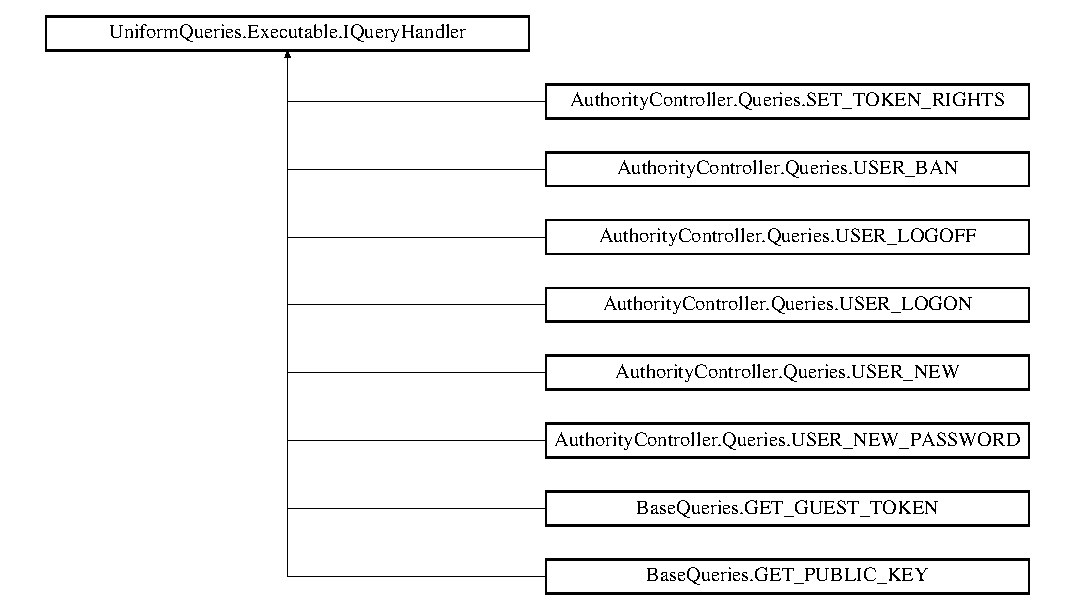
\includegraphics[height=7.753846cm]{d2/d1b/interface_uniform_queries_1_1_executable_1_1_i_query_handler}
\end{center}
\end{figure}
\subsection*{Public Member Functions}
\begin{DoxyCompactItemize}
\item 
void \mbox{\hyperlink{interface_uniform_queries_1_1_executable_1_1_i_query_handler_a3268d72c0388f5e3debba4d73bdfe523}{Execute}} (\mbox{\hyperlink{struct_uniform_queries_1_1_query_part}{Query\+Part}}\mbox{[}$\,$\mbox{]} query\+Parts)
\begin{DoxyCompactList}\small\item\em Methods that process query. \end{DoxyCompactList}\item 
bool \mbox{\hyperlink{interface_uniform_queries_1_1_executable_1_1_i_query_handler_a0f43184bf3e306a7cbebc39098f044ee}{Is\+Target}} (\mbox{\hyperlink{struct_uniform_queries_1_1_query_part}{Query\+Part}}\mbox{[}$\,$\mbox{]} query\+Parts)
\begin{DoxyCompactList}\small\item\em Check by the entry params does it target Query Handler. \end{DoxyCompactList}\item 
string \mbox{\hyperlink{interface_uniform_queries_1_1_executable_1_1_i_query_handler_ae0e55919571d5456af31298394d241a9}{Description}} (string culture\+Key)
\begin{DoxyCompactList}\small\item\em Return the description relative to the lenguage code or default if not found. \end{DoxyCompactList}\end{DoxyCompactItemize}


\subsection{Detailed Description}
All classes that implements this interface will automaticly detected by Queries\+A\+PI via first use and connected to queries processing. 



\subsection{Member Function Documentation}
\mbox{\Hypertarget{interface_uniform_queries_1_1_executable_1_1_i_query_handler_ae0e55919571d5456af31298394d241a9}\label{interface_uniform_queries_1_1_executable_1_1_i_query_handler_ae0e55919571d5456af31298394d241a9}} 
\index{Uniform\+Queries\+::\+Executable\+::\+I\+Query\+Handler@{Uniform\+Queries\+::\+Executable\+::\+I\+Query\+Handler}!Description@{Description}}
\index{Description@{Description}!Uniform\+Queries\+::\+Executable\+::\+I\+Query\+Handler@{Uniform\+Queries\+::\+Executable\+::\+I\+Query\+Handler}}
\subsubsection{\texorpdfstring{Description()}{Description()}}
{\footnotesize\ttfamily string Uniform\+Queries.\+Executable.\+I\+Query\+Handler.\+Description (\begin{DoxyParamCaption}\item[{string}]{culture\+Key }\end{DoxyParamCaption})}



Return the description relative to the lenguage code or default if not found. 


\begin{DoxyParams}{Parameters}
{\em culture\+Key} & \\
\hline
\end{DoxyParams}
\begin{DoxyReturn}{Returns}

\end{DoxyReturn}


Implemented in \mbox{\hyperlink{class_authority_controller_1_1_queries_1_1_u_s_e_r___l_o_g_o_n_af448426be46032c3ae103cdf4ea5f40b}{Authority\+Controller.\+Queries.\+U\+S\+E\+R\+\_\+\+L\+O\+G\+ON}}, \mbox{\hyperlink{class_authority_controller_1_1_queries_1_1_s_e_t___t_o_k_e_n___r_i_g_h_t_s_a149fb8950cf0ebbcb47b6a238c6458d2}{Authority\+Controller.\+Queries.\+S\+E\+T\+\_\+\+T\+O\+K\+E\+N\+\_\+\+R\+I\+G\+H\+TS}}, \mbox{\hyperlink{class_authority_controller_1_1_queries_1_1_g_e_t___g_u_e_s_t___t_o_k_e_n_a72902cb3b94f31ec4f8e6cd0bb1f2ed8}{Authority\+Controller.\+Queries.\+G\+E\+T\+\_\+\+G\+U\+E\+S\+T\+\_\+\+T\+O\+K\+EN}}, \mbox{\hyperlink{class_uniform_server_1_1_queries_1_1_g_e_t___p_u_b_l_i_c___k_e_y_aee414e6882494609ed576f061d662dc2}{Uniform\+Server.\+Queries.\+G\+E\+T\+\_\+\+P\+U\+B\+L\+I\+C\+\_\+\+K\+EY}}, \mbox{\hyperlink{class_authority_controller_1_1_queries_1_1_u_s_e_r___b_a_n_a0635966a71b389cbb4354e61e3c52513}{Authority\+Controller.\+Queries.\+U\+S\+E\+R\+\_\+\+B\+AN}}, \mbox{\hyperlink{class_authority_controller_1_1_queries_1_1_u_s_e_r___n_e_w_ab0995d0559e0033ea963acaccb6e37bf}{Authority\+Controller.\+Queries.\+U\+S\+E\+R\+\_\+\+N\+EW}}, \mbox{\hyperlink{class_authority_controller_1_1_queries_1_1_u_s_e_r___n_e_w___p_a_s_s_w_o_r_d_a04d2af1732d4ac353076d489fe75c696}{Authority\+Controller.\+Queries.\+U\+S\+E\+R\+\_\+\+N\+E\+W\+\_\+\+P\+A\+S\+S\+W\+O\+RD}}, and \mbox{\hyperlink{class_authority_controller_1_1_queries_1_1_u_s_e_r___l_o_g_o_f_f_a2cb738d74699241341b691cc55b57e1d}{Authority\+Controller.\+Queries.\+U\+S\+E\+R\+\_\+\+L\+O\+G\+O\+FF}}.

\mbox{\Hypertarget{interface_uniform_queries_1_1_executable_1_1_i_query_handler_a3268d72c0388f5e3debba4d73bdfe523}\label{interface_uniform_queries_1_1_executable_1_1_i_query_handler_a3268d72c0388f5e3debba4d73bdfe523}} 
\index{Uniform\+Queries\+::\+Executable\+::\+I\+Query\+Handler@{Uniform\+Queries\+::\+Executable\+::\+I\+Query\+Handler}!Execute@{Execute}}
\index{Execute@{Execute}!Uniform\+Queries\+::\+Executable\+::\+I\+Query\+Handler@{Uniform\+Queries\+::\+Executable\+::\+I\+Query\+Handler}}
\subsubsection{\texorpdfstring{Execute()}{Execute()}}
{\footnotesize\ttfamily void Uniform\+Queries.\+Executable.\+I\+Query\+Handler.\+Execute (\begin{DoxyParamCaption}\item[{\mbox{\hyperlink{struct_uniform_queries_1_1_query_part}{Query\+Part}} \mbox{[}$\,$\mbox{]}}]{query\+Parts }\end{DoxyParamCaption})}



Methods that process query. 


\begin{DoxyParams}{Parameters}
{\em query\+Parts} & \\
\hline
\end{DoxyParams}


Implemented in \mbox{\hyperlink{class_authority_controller_1_1_queries_1_1_u_s_e_r___l_o_g_o_n_a001f81c71597259636be777078e50f7e}{Authority\+Controller.\+Queries.\+U\+S\+E\+R\+\_\+\+L\+O\+G\+ON}}, \mbox{\hyperlink{class_authority_controller_1_1_queries_1_1_s_e_t___t_o_k_e_n___r_i_g_h_t_s_aebb323c8033e3a027f59c55a95695360}{Authority\+Controller.\+Queries.\+S\+E\+T\+\_\+\+T\+O\+K\+E\+N\+\_\+\+R\+I\+G\+H\+TS}}, \mbox{\hyperlink{class_authority_controller_1_1_queries_1_1_u_s_e_r___n_e_w___p_a_s_s_w_o_r_d_a63a5424c90f45f09f72a530ef0389416}{Authority\+Controller.\+Queries.\+U\+S\+E\+R\+\_\+\+N\+E\+W\+\_\+\+P\+A\+S\+S\+W\+O\+RD}}, \mbox{\hyperlink{class_authority_controller_1_1_queries_1_1_g_e_t___g_u_e_s_t___t_o_k_e_n_a99b0dddf4ff45771e546ec0fa14b0aae}{Authority\+Controller.\+Queries.\+G\+E\+T\+\_\+\+G\+U\+E\+S\+T\+\_\+\+T\+O\+K\+EN}}, \mbox{\hyperlink{class_uniform_server_1_1_queries_1_1_g_e_t___p_u_b_l_i_c___k_e_y_a63367fa9543a3fb4a1126373a833c317}{Uniform\+Server.\+Queries.\+G\+E\+T\+\_\+\+P\+U\+B\+L\+I\+C\+\_\+\+K\+EY}}, \mbox{\hyperlink{class_authority_controller_1_1_queries_1_1_u_s_e_r___b_a_n_a719795c950c9dedbc187c2c0cfca37a7}{Authority\+Controller.\+Queries.\+U\+S\+E\+R\+\_\+\+B\+AN}}, \mbox{\hyperlink{class_authority_controller_1_1_queries_1_1_u_s_e_r___n_e_w_afd715fb3d60e53ca7e3d55a4433f529c}{Authority\+Controller.\+Queries.\+U\+S\+E\+R\+\_\+\+N\+EW}}, and \mbox{\hyperlink{class_authority_controller_1_1_queries_1_1_u_s_e_r___l_o_g_o_f_f_a2e4d5a0f8ee93210522c41a38adbcce2}{Authority\+Controller.\+Queries.\+U\+S\+E\+R\+\_\+\+L\+O\+G\+O\+FF}}.

\mbox{\Hypertarget{interface_uniform_queries_1_1_executable_1_1_i_query_handler_a0f43184bf3e306a7cbebc39098f044ee}\label{interface_uniform_queries_1_1_executable_1_1_i_query_handler_a0f43184bf3e306a7cbebc39098f044ee}} 
\index{Uniform\+Queries\+::\+Executable\+::\+I\+Query\+Handler@{Uniform\+Queries\+::\+Executable\+::\+I\+Query\+Handler}!Is\+Target@{Is\+Target}}
\index{Is\+Target@{Is\+Target}!Uniform\+Queries\+::\+Executable\+::\+I\+Query\+Handler@{Uniform\+Queries\+::\+Executable\+::\+I\+Query\+Handler}}
\subsubsection{\texorpdfstring{Is\+Target()}{IsTarget()}}
{\footnotesize\ttfamily bool Uniform\+Queries.\+Executable.\+I\+Query\+Handler.\+Is\+Target (\begin{DoxyParamCaption}\item[{\mbox{\hyperlink{struct_uniform_queries_1_1_query_part}{Query\+Part}} \mbox{[}$\,$\mbox{]}}]{query\+Parts }\end{DoxyParamCaption})}



Check by the entry params does it target Query Handler. 


\begin{DoxyParams}{Parameters}
{\em query\+Parts} & \\
\hline
\end{DoxyParams}
\begin{DoxyReturn}{Returns}

\end{DoxyReturn}


Implemented in \mbox{\hyperlink{class_authority_controller_1_1_queries_1_1_u_s_e_r___n_e_w_a6e26596b5a5ecc3d07591766b5d325ec}{Authority\+Controller.\+Queries.\+U\+S\+E\+R\+\_\+\+N\+EW}}, \mbox{\hyperlink{class_authority_controller_1_1_queries_1_1_u_s_e_r___n_e_w___p_a_s_s_w_o_r_d_a48ff6874453caf45973ad386bfe5b513}{Authority\+Controller.\+Queries.\+U\+S\+E\+R\+\_\+\+N\+E\+W\+\_\+\+P\+A\+S\+S\+W\+O\+RD}}, \mbox{\hyperlink{class_authority_controller_1_1_queries_1_1_u_s_e_r___b_a_n_a29c898b411adc3a0edbed31cf90e007b}{Authority\+Controller.\+Queries.\+U\+S\+E\+R\+\_\+\+B\+AN}}, \mbox{\hyperlink{class_authority_controller_1_1_queries_1_1_u_s_e_r___l_o_g_o_n_a53261c6c60dc1a2324a67adf19f7547a}{Authority\+Controller.\+Queries.\+U\+S\+E\+R\+\_\+\+L\+O\+G\+ON}}, \mbox{\hyperlink{class_authority_controller_1_1_queries_1_1_s_e_t___t_o_k_e_n___r_i_g_h_t_s_a605feed66d357dc93ccc825068d83c96}{Authority\+Controller.\+Queries.\+S\+E\+T\+\_\+\+T\+O\+K\+E\+N\+\_\+\+R\+I\+G\+H\+TS}}, \mbox{\hyperlink{class_authority_controller_1_1_queries_1_1_u_s_e_r___l_o_g_o_f_f_afbfa78117d68ab2bd2728c78d31c1c58}{Authority\+Controller.\+Queries.\+U\+S\+E\+R\+\_\+\+L\+O\+G\+O\+FF}}, \mbox{\hyperlink{class_uniform_server_1_1_queries_1_1_g_e_t___p_u_b_l_i_c___k_e_y_ae27d462fe9ccbbf22ac03c9ead9cbe8f}{Uniform\+Server.\+Queries.\+G\+E\+T\+\_\+\+P\+U\+B\+L\+I\+C\+\_\+\+K\+EY}}, and \mbox{\hyperlink{class_authority_controller_1_1_queries_1_1_g_e_t___g_u_e_s_t___t_o_k_e_n_a5606c5797e0a684a6bfbbd851f186268}{Authority\+Controller.\+Queries.\+G\+E\+T\+\_\+\+G\+U\+E\+S\+T\+\_\+\+T\+O\+K\+EN}}.



The documentation for this interface was generated from the following file\+:\begin{DoxyCompactItemize}
\item 
D\+:/\+Work/\+Git\+Hub/doloro-\/networking-\/framework/\+Core/\+Uniform\+Queries/\+Exacutable/I\+Query\+Handler.\+cs\end{DoxyCompactItemize}

\hypertarget{class_authority_controller_1_1_a_p_i_1_1_local_users}{}\section{Authority\+Controller.\+A\+P\+I.\+Local\+Users Class Reference}
\label{class_authority_controller_1_1_a_p_i_1_1_local_users}\index{Authority\+Controller.\+A\+P\+I.\+Local\+Users@{Authority\+Controller.\+A\+P\+I.\+Local\+Users}}


\mbox{\hyperlink{namespace_authority_controller_1_1_a_p_i}{A\+PI}} that provide operation with authority data stored on local machine out of Uniform\+Data\+Operator storage.  


\subsection*{Static Public Member Functions}
\begin{DoxyCompactItemize}
\item 
static async void \mbox{\hyperlink{class_authority_controller_1_1_a_p_i_1_1_local_users_a1c037e720aa8b718fa5ceec4d2495f41}{Load\+Profiles\+Async}} (string directory)
\begin{DoxyCompactList}\small\item\em Loading users data from directory. \end{DoxyCompactList}\item 
static void \mbox{\hyperlink{class_authority_controller_1_1_a_p_i_1_1_local_users_ac9295cdceab3bc5a0363a435cbdf3f03}{Set\+Profile}} (\mbox{\hyperlink{class_authority_controller_1_1_data_1_1_personal_1_1_user}{User}} user)
\begin{DoxyCompactList}\small\item\em Adding user\textquotesingle{}s profile by directory sete up via config file. \end{DoxyCompactList}\item 
static async void \mbox{\hyperlink{class_authority_controller_1_1_a_p_i_1_1_local_users_a87fd101098bce03f6c0775434946640e}{Set\+Profile\+Async}} (\mbox{\hyperlink{class_authority_controller_1_1_data_1_1_personal_1_1_user}{User}} user, string directory)
\begin{DoxyCompactList}\small\item\em Adding user\textquotesingle{}s profile by directory. \end{DoxyCompactList}\item 
static bool \mbox{\hyperlink{class_authority_controller_1_1_a_p_i_1_1_local_users_af2f5f3adeecfe6de4d7e480dfc22157a}{Set\+Profile}} (\mbox{\hyperlink{class_authority_controller_1_1_data_1_1_personal_1_1_user}{User}} user, string directory)
\begin{DoxyCompactList}\small\item\em Adding user\textquotesingle{}s profile by directory. \end{DoxyCompactList}\item 
static bool \mbox{\hyperlink{class_authority_controller_1_1_a_p_i_1_1_local_users_a11f2205f650c36ae8bce9b291a6f1cba}{Remove\+Profile}} (\mbox{\hyperlink{class_authority_controller_1_1_data_1_1_personal_1_1_user}{User}} user)
\begin{DoxyCompactList}\small\item\em Remove user profile from directory seted up via Config file. \end{DoxyCompactList}\item 
static bool \mbox{\hyperlink{class_authority_controller_1_1_a_p_i_1_1_local_users_ae02de90abedf4b3e97478dc6270d833d}{Remove\+Profile}} (\mbox{\hyperlink{class_authority_controller_1_1_data_1_1_personal_1_1_user}{User}} user, string directory)
\begin{DoxyCompactList}\small\item\em Remove user profile from directory. \end{DoxyCompactList}\item 
static uint \mbox{\hyperlink{class_authority_controller_1_1_a_p_i_1_1_local_users_aad5081adb0650b6d693e00bf0e833a8a}{Generate\+ID}} (\mbox{\hyperlink{class_authority_controller_1_1_data_1_1_personal_1_1_user}{User}} user)
\begin{DoxyCompactList}\small\item\em Looking for free id. \end{DoxyCompactList}\item 
static void \mbox{\hyperlink{class_authority_controller_1_1_a_p_i_1_1_local_users_a2090f668f0dcc303c254b0bdac6c0701}{Add\+To\+Loaded\+Data}} (\mbox{\hyperlink{class_authority_controller_1_1_data_1_1_personal_1_1_user}{User}} user)
\begin{DoxyCompactList}\small\item\em Registrate user in tables by id and login. \end{DoxyCompactList}\item 
static void \mbox{\hyperlink{class_authority_controller_1_1_a_p_i_1_1_local_users_a38dbb5226a8c8fb138f6ecb590713d75}{Clear\+Users\+Loaded\+Data}} ()
\begin{DoxyCompactList}\small\item\em Remove all loaded users data. \end{DoxyCompactList}\item 
static bool \mbox{\hyperlink{class_authority_controller_1_1_a_p_i_1_1_local_users_a9ce59e22a9d7f732ea20d2579ab57f48}{Try\+To\+Find\+User}} (uint id, out \mbox{\hyperlink{class_authority_controller_1_1_data_1_1_personal_1_1_user}{User}} user)
\begin{DoxyCompactList}\small\item\em Try to find user by ID in loaded users table. \end{DoxyCompactList}\item 
static bool \mbox{\hyperlink{class_authority_controller_1_1_a_p_i_1_1_local_users_af37939b7ade7b7be30f5ad8935cecdb3}{Try\+To\+Find\+User}} (string login, out \mbox{\hyperlink{class_authority_controller_1_1_data_1_1_personal_1_1_user}{User}} user)
\begin{DoxyCompactList}\small\item\em Try to find user by ID in loaded users table. \end{DoxyCompactList}\item 
static bool \mbox{\hyperlink{class_authority_controller_1_1_a_p_i_1_1_local_users_a8bf53e0c8216de0a8f5244e11ccb90b5}{Try\+To\+Find\+User\+Uniform}} (string uniform\+Value, out \mbox{\hyperlink{class_authority_controller_1_1_data_1_1_personal_1_1_user}{User}} user\+Profile, out string error)
\begin{DoxyCompactList}\small\item\em Seeking for user. \end{DoxyCompactList}\end{DoxyCompactItemize}
\subsection*{Properties}
\begin{DoxyCompactItemize}
\item 
static bool \mbox{\hyperlink{class_authority_controller_1_1_a_p_i_1_1_local_users_afdfecc5fc12d8f2a862ddc030577a064}{Has\+Async\+Loadings}}\hspace{0.3cm}{\ttfamily  \mbox{[}get\mbox{]}}
\begin{DoxyCompactList}\small\item\em Does async processes started at the moment? \end{DoxyCompactList}\end{DoxyCompactItemize}
\subsection*{Events}
\begin{DoxyCompactItemize}
\item 
static System.\+Action$<$ string, int, int $>$ \mbox{\hyperlink{class_authority_controller_1_1_a_p_i_1_1_local_users_a54370dd6dd474a14106891cd6d0beaaf}{Directory\+Loading\+Finished}}
\begin{DoxyCompactList}\small\item\em Event that will be called when loading of users from directory will be finished. Int -\/ count of loaded files. Int -\/ count of corupted files. \end{DoxyCompactList}\item 
static System.\+Action$<$ \mbox{\hyperlink{class_authority_controller_1_1_data_1_1_personal_1_1_user}{User}} $>$ \mbox{\hyperlink{class_authority_controller_1_1_a_p_i_1_1_local_users_af973c97a05818a9e360aadca02da8834}{User\+Profile\+Stored}}
\begin{DoxyCompactList}\small\item\em Event that will be called when profile will be setted to storage. \end{DoxyCompactList}\item 
static System.\+Action$<$ \mbox{\hyperlink{class_authority_controller_1_1_data_1_1_personal_1_1_user}{User}}, string $>$ \mbox{\hyperlink{class_authority_controller_1_1_a_p_i_1_1_local_users_af05c837a76c7b94631884b965e5cc75d}{User\+Profile\+Not\+Stored}}
\begin{DoxyCompactList}\small\item\em Event that will be called when profile will be fail adding to storage. \end{DoxyCompactList}\end{DoxyCompactItemize}
\subsection*{Static Private Member Functions}
\begin{DoxyCompactItemize}
\item 
static string \mbox{\hyperlink{class_authority_controller_1_1_a_p_i_1_1_local_users_a67fe99b2249aacec99b18538ee86bec8}{Get\+User\+File\+Name}} (\mbox{\hyperlink{class_authority_controller_1_1_data_1_1_personal_1_1_user}{User}} user)
\begin{DoxyCompactList}\small\item\em Return unified name based on user\textquotesingle{}s profile. \end{DoxyCompactList}\end{DoxyCompactItemize}
\subsection*{Static Private Attributes}
\begin{DoxyCompactItemize}
\item 
static readonly Hashtable \mbox{\hyperlink{class_authority_controller_1_1_a_p_i_1_1_local_users_aaae0c59c3cdaf7fcde412e10326059f1}{Users\+By\+Login}} = new Hashtable()
\begin{DoxyCompactList}\small\item\em Table that provide aaccess to user data by login. \end{DoxyCompactList}\item 
static readonly Hashtable \mbox{\hyperlink{class_authority_controller_1_1_a_p_i_1_1_local_users_a7ccc07a39b84ca1871e981bf6f8729ba}{Users\+By\+Id}} = new Hashtable()
\begin{DoxyCompactList}\small\item\em Table that provide access to user by unique ID. \end{DoxyCompactList}\item 
static readonly Hash\+Set$<$ string $>$ \mbox{\hyperlink{class_authority_controller_1_1_a_p_i_1_1_local_users_a6d00e6327f737d23cfdfff3f13ecaec3}{Loading\+Locked\+Directories}} = new Hash\+Set$<$string$>$()
\begin{DoxyCompactList}\small\item\em Contains directories that has users loading process and blocked for new ones. \end{DoxyCompactList}\end{DoxyCompactItemize}


\subsection{Detailed Description}
\mbox{\hyperlink{namespace_authority_controller_1_1_a_p_i}{A\+PI}} that provide operation with authority data stored on local machine out of Uniform\+Data\+Operator storage. 



\subsection{Member Function Documentation}
\mbox{\Hypertarget{class_authority_controller_1_1_a_p_i_1_1_local_users_a2090f668f0dcc303c254b0bdac6c0701}\label{class_authority_controller_1_1_a_p_i_1_1_local_users_a2090f668f0dcc303c254b0bdac6c0701}} 
\index{Authority\+Controller\+::\+A\+P\+I\+::\+Local\+Users@{Authority\+Controller\+::\+A\+P\+I\+::\+Local\+Users}!Add\+To\+Loaded\+Data@{Add\+To\+Loaded\+Data}}
\index{Add\+To\+Loaded\+Data@{Add\+To\+Loaded\+Data}!Authority\+Controller\+::\+A\+P\+I\+::\+Local\+Users@{Authority\+Controller\+::\+A\+P\+I\+::\+Local\+Users}}
\subsubsection{\texorpdfstring{Add\+To\+Loaded\+Data()}{AddToLoadedData()}}
{\footnotesize\ttfamily static void Authority\+Controller.\+A\+P\+I.\+Local\+Users.\+Add\+To\+Loaded\+Data (\begin{DoxyParamCaption}\item[{\mbox{\hyperlink{class_authority_controller_1_1_data_1_1_personal_1_1_user}{User}}}]{user }\end{DoxyParamCaption})\hspace{0.3cm}{\ttfamily [static]}}



Registrate user in tables by id and login. 


\begin{DoxyParams}{Parameters}
{\em user} & \\
\hline
\end{DoxyParams}
\mbox{\Hypertarget{class_authority_controller_1_1_a_p_i_1_1_local_users_a38dbb5226a8c8fb138f6ecb590713d75}\label{class_authority_controller_1_1_a_p_i_1_1_local_users_a38dbb5226a8c8fb138f6ecb590713d75}} 
\index{Authority\+Controller\+::\+A\+P\+I\+::\+Local\+Users@{Authority\+Controller\+::\+A\+P\+I\+::\+Local\+Users}!Clear\+Users\+Loaded\+Data@{Clear\+Users\+Loaded\+Data}}
\index{Clear\+Users\+Loaded\+Data@{Clear\+Users\+Loaded\+Data}!Authority\+Controller\+::\+A\+P\+I\+::\+Local\+Users@{Authority\+Controller\+::\+A\+P\+I\+::\+Local\+Users}}
\subsubsection{\texorpdfstring{Clear\+Users\+Loaded\+Data()}{ClearUsersLoadedData()}}
{\footnotesize\ttfamily static void Authority\+Controller.\+A\+P\+I.\+Local\+Users.\+Clear\+Users\+Loaded\+Data (\begin{DoxyParamCaption}{ }\end{DoxyParamCaption})\hspace{0.3cm}{\ttfamily [static]}}



Remove all loaded users data. 

\mbox{\Hypertarget{class_authority_controller_1_1_a_p_i_1_1_local_users_aad5081adb0650b6d693e00bf0e833a8a}\label{class_authority_controller_1_1_a_p_i_1_1_local_users_aad5081adb0650b6d693e00bf0e833a8a}} 
\index{Authority\+Controller\+::\+A\+P\+I\+::\+Local\+Users@{Authority\+Controller\+::\+A\+P\+I\+::\+Local\+Users}!Generate\+ID@{Generate\+ID}}
\index{Generate\+ID@{Generate\+ID}!Authority\+Controller\+::\+A\+P\+I\+::\+Local\+Users@{Authority\+Controller\+::\+A\+P\+I\+::\+Local\+Users}}
\subsubsection{\texorpdfstring{Generate\+I\+D()}{GenerateID()}}
{\footnotesize\ttfamily static uint Authority\+Controller.\+A\+P\+I.\+Local\+Users.\+Generate\+ID (\begin{DoxyParamCaption}\item[{\mbox{\hyperlink{class_authority_controller_1_1_data_1_1_personal_1_1_user}{User}}}]{user }\end{DoxyParamCaption})\hspace{0.3cm}{\ttfamily [static]}}



Looking for free id. 


\begin{DoxyParams}{Parameters}
{\em user} & \\
\hline
\end{DoxyParams}
\begin{DoxyReturn}{Returns}

\end{DoxyReturn}
\mbox{\Hypertarget{class_authority_controller_1_1_a_p_i_1_1_local_users_a67fe99b2249aacec99b18538ee86bec8}\label{class_authority_controller_1_1_a_p_i_1_1_local_users_a67fe99b2249aacec99b18538ee86bec8}} 
\index{Authority\+Controller\+::\+A\+P\+I\+::\+Local\+Users@{Authority\+Controller\+::\+A\+P\+I\+::\+Local\+Users}!Get\+User\+File\+Name@{Get\+User\+File\+Name}}
\index{Get\+User\+File\+Name@{Get\+User\+File\+Name}!Authority\+Controller\+::\+A\+P\+I\+::\+Local\+Users@{Authority\+Controller\+::\+A\+P\+I\+::\+Local\+Users}}
\subsubsection{\texorpdfstring{Get\+User\+File\+Name()}{GetUserFileName()}}
{\footnotesize\ttfamily static string Authority\+Controller.\+A\+P\+I.\+Local\+Users.\+Get\+User\+File\+Name (\begin{DoxyParamCaption}\item[{\mbox{\hyperlink{class_authority_controller_1_1_data_1_1_personal_1_1_user}{User}}}]{user }\end{DoxyParamCaption})\hspace{0.3cm}{\ttfamily [static]}, {\ttfamily [private]}}



Return unified name based on user\textquotesingle{}s profile. 


\begin{DoxyParams}{Parameters}
{\em user} & \\
\hline
\end{DoxyParams}
\begin{DoxyReturn}{Returns}

\end{DoxyReturn}
\mbox{\Hypertarget{class_authority_controller_1_1_a_p_i_1_1_local_users_a1c037e720aa8b718fa5ceec4d2495f41}\label{class_authority_controller_1_1_a_p_i_1_1_local_users_a1c037e720aa8b718fa5ceec4d2495f41}} 
\index{Authority\+Controller\+::\+A\+P\+I\+::\+Local\+Users@{Authority\+Controller\+::\+A\+P\+I\+::\+Local\+Users}!Load\+Profiles\+Async@{Load\+Profiles\+Async}}
\index{Load\+Profiles\+Async@{Load\+Profiles\+Async}!Authority\+Controller\+::\+A\+P\+I\+::\+Local\+Users@{Authority\+Controller\+::\+A\+P\+I\+::\+Local\+Users}}
\subsubsection{\texorpdfstring{Load\+Profiles\+Async()}{LoadProfilesAsync()}}
{\footnotesize\ttfamily static async void Authority\+Controller.\+A\+P\+I.\+Local\+Users.\+Load\+Profiles\+Async (\begin{DoxyParamCaption}\item[{string}]{directory }\end{DoxyParamCaption})\hspace{0.3cm}{\ttfamily [static]}}



Loading users data from directory. 


\begin{DoxyParams}{Parameters}
{\em directory} & \\
\hline
\end{DoxyParams}
\mbox{\Hypertarget{class_authority_controller_1_1_a_p_i_1_1_local_users_a11f2205f650c36ae8bce9b291a6f1cba}\label{class_authority_controller_1_1_a_p_i_1_1_local_users_a11f2205f650c36ae8bce9b291a6f1cba}} 
\index{Authority\+Controller\+::\+A\+P\+I\+::\+Local\+Users@{Authority\+Controller\+::\+A\+P\+I\+::\+Local\+Users}!Remove\+Profile@{Remove\+Profile}}
\index{Remove\+Profile@{Remove\+Profile}!Authority\+Controller\+::\+A\+P\+I\+::\+Local\+Users@{Authority\+Controller\+::\+A\+P\+I\+::\+Local\+Users}}
\subsubsection{\texorpdfstring{Remove\+Profile()}{RemoveProfile()}\hspace{0.1cm}{\footnotesize\ttfamily [1/2]}}
{\footnotesize\ttfamily static bool Authority\+Controller.\+A\+P\+I.\+Local\+Users.\+Remove\+Profile (\begin{DoxyParamCaption}\item[{\mbox{\hyperlink{class_authority_controller_1_1_data_1_1_personal_1_1_user}{User}}}]{user }\end{DoxyParamCaption})\hspace{0.3cm}{\ttfamily [static]}}



Remove user profile from directory seted up via Config file. 


\begin{DoxyParams}{Parameters}
{\em user} & \\
\hline
\end{DoxyParams}
\mbox{\Hypertarget{class_authority_controller_1_1_a_p_i_1_1_local_users_ae02de90abedf4b3e97478dc6270d833d}\label{class_authority_controller_1_1_a_p_i_1_1_local_users_ae02de90abedf4b3e97478dc6270d833d}} 
\index{Authority\+Controller\+::\+A\+P\+I\+::\+Local\+Users@{Authority\+Controller\+::\+A\+P\+I\+::\+Local\+Users}!Remove\+Profile@{Remove\+Profile}}
\index{Remove\+Profile@{Remove\+Profile}!Authority\+Controller\+::\+A\+P\+I\+::\+Local\+Users@{Authority\+Controller\+::\+A\+P\+I\+::\+Local\+Users}}
\subsubsection{\texorpdfstring{Remove\+Profile()}{RemoveProfile()}\hspace{0.1cm}{\footnotesize\ttfamily [2/2]}}
{\footnotesize\ttfamily static bool Authority\+Controller.\+A\+P\+I.\+Local\+Users.\+Remove\+Profile (\begin{DoxyParamCaption}\item[{\mbox{\hyperlink{class_authority_controller_1_1_data_1_1_personal_1_1_user}{User}}}]{user,  }\item[{string}]{directory }\end{DoxyParamCaption})\hspace{0.3cm}{\ttfamily [static]}}



Remove user profile from directory. 


\begin{DoxyParams}{Parameters}
{\em user} & \\
\hline
{\em directory} & \\
\hline
\end{DoxyParams}
\mbox{\Hypertarget{class_authority_controller_1_1_a_p_i_1_1_local_users_ac9295cdceab3bc5a0363a435cbdf3f03}\label{class_authority_controller_1_1_a_p_i_1_1_local_users_ac9295cdceab3bc5a0363a435cbdf3f03}} 
\index{Authority\+Controller\+::\+A\+P\+I\+::\+Local\+Users@{Authority\+Controller\+::\+A\+P\+I\+::\+Local\+Users}!Set\+Profile@{Set\+Profile}}
\index{Set\+Profile@{Set\+Profile}!Authority\+Controller\+::\+A\+P\+I\+::\+Local\+Users@{Authority\+Controller\+::\+A\+P\+I\+::\+Local\+Users}}
\subsubsection{\texorpdfstring{Set\+Profile()}{SetProfile()}\hspace{0.1cm}{\footnotesize\ttfamily [1/2]}}
{\footnotesize\ttfamily static void Authority\+Controller.\+A\+P\+I.\+Local\+Users.\+Set\+Profile (\begin{DoxyParamCaption}\item[{\mbox{\hyperlink{class_authority_controller_1_1_data_1_1_personal_1_1_user}{User}}}]{user }\end{DoxyParamCaption})\hspace{0.3cm}{\ttfamily [static]}}



Adding user\textquotesingle{}s profile by directory sete up via config file. 


\begin{DoxyParams}{Parameters}
{\em user} & User profile.\\
\hline
\end{DoxyParams}
\mbox{\Hypertarget{class_authority_controller_1_1_a_p_i_1_1_local_users_af2f5f3adeecfe6de4d7e480dfc22157a}\label{class_authority_controller_1_1_a_p_i_1_1_local_users_af2f5f3adeecfe6de4d7e480dfc22157a}} 
\index{Authority\+Controller\+::\+A\+P\+I\+::\+Local\+Users@{Authority\+Controller\+::\+A\+P\+I\+::\+Local\+Users}!Set\+Profile@{Set\+Profile}}
\index{Set\+Profile@{Set\+Profile}!Authority\+Controller\+::\+A\+P\+I\+::\+Local\+Users@{Authority\+Controller\+::\+A\+P\+I\+::\+Local\+Users}}
\subsubsection{\texorpdfstring{Set\+Profile()}{SetProfile()}\hspace{0.1cm}{\footnotesize\ttfamily [2/2]}}
{\footnotesize\ttfamily static bool Authority\+Controller.\+A\+P\+I.\+Local\+Users.\+Set\+Profile (\begin{DoxyParamCaption}\item[{\mbox{\hyperlink{class_authority_controller_1_1_data_1_1_personal_1_1_user}{User}}}]{user,  }\item[{string}]{directory }\end{DoxyParamCaption})\hspace{0.3cm}{\ttfamily [static]}}



Adding user\textquotesingle{}s profile by directory. 


\begin{DoxyParams}{Parameters}
{\em user} & User profile.\\
\hline
{\em directory} & Users storage.\\
\hline
\end{DoxyParams}
\mbox{\Hypertarget{class_authority_controller_1_1_a_p_i_1_1_local_users_a87fd101098bce03f6c0775434946640e}\label{class_authority_controller_1_1_a_p_i_1_1_local_users_a87fd101098bce03f6c0775434946640e}} 
\index{Authority\+Controller\+::\+A\+P\+I\+::\+Local\+Users@{Authority\+Controller\+::\+A\+P\+I\+::\+Local\+Users}!Set\+Profile\+Async@{Set\+Profile\+Async}}
\index{Set\+Profile\+Async@{Set\+Profile\+Async}!Authority\+Controller\+::\+A\+P\+I\+::\+Local\+Users@{Authority\+Controller\+::\+A\+P\+I\+::\+Local\+Users}}
\subsubsection{\texorpdfstring{Set\+Profile\+Async()}{SetProfileAsync()}}
{\footnotesize\ttfamily static async void Authority\+Controller.\+A\+P\+I.\+Local\+Users.\+Set\+Profile\+Async (\begin{DoxyParamCaption}\item[{\mbox{\hyperlink{class_authority_controller_1_1_data_1_1_personal_1_1_user}{User}}}]{user,  }\item[{string}]{directory }\end{DoxyParamCaption})\hspace{0.3cm}{\ttfamily [static]}}



Adding user\textquotesingle{}s profile by directory. 


\begin{DoxyParams}{Parameters}
{\em user} & User profile.\\
\hline
{\em directory} & Users storage.\\
\hline
\end{DoxyParams}
\mbox{\Hypertarget{class_authority_controller_1_1_a_p_i_1_1_local_users_a9ce59e22a9d7f732ea20d2579ab57f48}\label{class_authority_controller_1_1_a_p_i_1_1_local_users_a9ce59e22a9d7f732ea20d2579ab57f48}} 
\index{Authority\+Controller\+::\+A\+P\+I\+::\+Local\+Users@{Authority\+Controller\+::\+A\+P\+I\+::\+Local\+Users}!Try\+To\+Find\+User@{Try\+To\+Find\+User}}
\index{Try\+To\+Find\+User@{Try\+To\+Find\+User}!Authority\+Controller\+::\+A\+P\+I\+::\+Local\+Users@{Authority\+Controller\+::\+A\+P\+I\+::\+Local\+Users}}
\subsubsection{\texorpdfstring{Try\+To\+Find\+User()}{TryToFindUser()}\hspace{0.1cm}{\footnotesize\ttfamily [1/2]}}
{\footnotesize\ttfamily static bool Authority\+Controller.\+A\+P\+I.\+Local\+Users.\+Try\+To\+Find\+User (\begin{DoxyParamCaption}\item[{uint}]{id,  }\item[{out \mbox{\hyperlink{class_authority_controller_1_1_data_1_1_personal_1_1_user}{User}}}]{user }\end{DoxyParamCaption})\hspace{0.3cm}{\ttfamily [static]}}



Try to find user by ID in loaded users table. 


\begin{DoxyParams}{Parameters}
{\em id} & Unique user\textquotesingle{}s id.\\
\hline
{\em user} & Reference on loaded user profile.\\
\hline
\end{DoxyParams}
\begin{DoxyReturn}{Returns}
Result of operation.
\end{DoxyReturn}
\mbox{\Hypertarget{class_authority_controller_1_1_a_p_i_1_1_local_users_af37939b7ade7b7be30f5ad8935cecdb3}\label{class_authority_controller_1_1_a_p_i_1_1_local_users_af37939b7ade7b7be30f5ad8935cecdb3}} 
\index{Authority\+Controller\+::\+A\+P\+I\+::\+Local\+Users@{Authority\+Controller\+::\+A\+P\+I\+::\+Local\+Users}!Try\+To\+Find\+User@{Try\+To\+Find\+User}}
\index{Try\+To\+Find\+User@{Try\+To\+Find\+User}!Authority\+Controller\+::\+A\+P\+I\+::\+Local\+Users@{Authority\+Controller\+::\+A\+P\+I\+::\+Local\+Users}}
\subsubsection{\texorpdfstring{Try\+To\+Find\+User()}{TryToFindUser()}\hspace{0.1cm}{\footnotesize\ttfamily [2/2]}}
{\footnotesize\ttfamily static bool Authority\+Controller.\+A\+P\+I.\+Local\+Users.\+Try\+To\+Find\+User (\begin{DoxyParamCaption}\item[{string}]{login,  }\item[{out \mbox{\hyperlink{class_authority_controller_1_1_data_1_1_personal_1_1_user}{User}}}]{user }\end{DoxyParamCaption})\hspace{0.3cm}{\ttfamily [static]}}



Try to find user by ID in loaded users table. 


\begin{DoxyParams}{Parameters}
{\em login} & Unique user\textquotesingle{}s login.\\
\hline
{\em user} & Reference on loaded user profile.\\
\hline
\end{DoxyParams}
\begin{DoxyReturn}{Returns}
Result of operation.
\end{DoxyReturn}
\mbox{\Hypertarget{class_authority_controller_1_1_a_p_i_1_1_local_users_a8bf53e0c8216de0a8f5244e11ccb90b5}\label{class_authority_controller_1_1_a_p_i_1_1_local_users_a8bf53e0c8216de0a8f5244e11ccb90b5}} 
\index{Authority\+Controller\+::\+A\+P\+I\+::\+Local\+Users@{Authority\+Controller\+::\+A\+P\+I\+::\+Local\+Users}!Try\+To\+Find\+User\+Uniform@{Try\+To\+Find\+User\+Uniform}}
\index{Try\+To\+Find\+User\+Uniform@{Try\+To\+Find\+User\+Uniform}!Authority\+Controller\+::\+A\+P\+I\+::\+Local\+Users@{Authority\+Controller\+::\+A\+P\+I\+::\+Local\+Users}}
\subsubsection{\texorpdfstring{Try\+To\+Find\+User\+Uniform()}{TryToFindUserUniform()}}
{\footnotesize\ttfamily static bool Authority\+Controller.\+A\+P\+I.\+Local\+Users.\+Try\+To\+Find\+User\+Uniform (\begin{DoxyParamCaption}\item[{string}]{uniform\+Value,  }\item[{out \mbox{\hyperlink{class_authority_controller_1_1_data_1_1_personal_1_1_user}{User}}}]{user\+Profile,  }\item[{out string}]{error }\end{DoxyParamCaption})\hspace{0.3cm}{\ttfamily [static]}}



Seeking for user. 


\begin{DoxyParams}{Parameters}
{\em uniform\+Value} & ID or login in string format.\\
\hline
{\em user\+Profile} & Field that will contain user\textquotesingle{}s profile in case of found.\\
\hline
{\em error} & Error that describe a reasone of fail. Could be send backward to client.\\
\hline
\end{DoxyParams}
\begin{DoxyReturn}{Returns}

\end{DoxyReturn}


\subsection{Member Data Documentation}
\mbox{\Hypertarget{class_authority_controller_1_1_a_p_i_1_1_local_users_a6d00e6327f737d23cfdfff3f13ecaec3}\label{class_authority_controller_1_1_a_p_i_1_1_local_users_a6d00e6327f737d23cfdfff3f13ecaec3}} 
\index{Authority\+Controller\+::\+A\+P\+I\+::\+Local\+Users@{Authority\+Controller\+::\+A\+P\+I\+::\+Local\+Users}!Loading\+Locked\+Directories@{Loading\+Locked\+Directories}}
\index{Loading\+Locked\+Directories@{Loading\+Locked\+Directories}!Authority\+Controller\+::\+A\+P\+I\+::\+Local\+Users@{Authority\+Controller\+::\+A\+P\+I\+::\+Local\+Users}}
\subsubsection{\texorpdfstring{Loading\+Locked\+Directories}{LoadingLockedDirectories}}
{\footnotesize\ttfamily readonly Hash\+Set$<$string$>$ Authority\+Controller.\+A\+P\+I.\+Local\+Users.\+Loading\+Locked\+Directories = new Hash\+Set$<$string$>$()\hspace{0.3cm}{\ttfamily [static]}, {\ttfamily [private]}}



Contains directories that has users loading process and blocked for new ones. 

\mbox{\Hypertarget{class_authority_controller_1_1_a_p_i_1_1_local_users_a7ccc07a39b84ca1871e981bf6f8729ba}\label{class_authority_controller_1_1_a_p_i_1_1_local_users_a7ccc07a39b84ca1871e981bf6f8729ba}} 
\index{Authority\+Controller\+::\+A\+P\+I\+::\+Local\+Users@{Authority\+Controller\+::\+A\+P\+I\+::\+Local\+Users}!Users\+By\+Id@{Users\+By\+Id}}
\index{Users\+By\+Id@{Users\+By\+Id}!Authority\+Controller\+::\+A\+P\+I\+::\+Local\+Users@{Authority\+Controller\+::\+A\+P\+I\+::\+Local\+Users}}
\subsubsection{\texorpdfstring{Users\+By\+Id}{UsersById}}
{\footnotesize\ttfamily readonly Hashtable Authority\+Controller.\+A\+P\+I.\+Local\+Users.\+Users\+By\+Id = new Hashtable()\hspace{0.3cm}{\ttfamily [static]}, {\ttfamily [private]}}



Table that provide access to user by unique ID. 

\mbox{\Hypertarget{class_authority_controller_1_1_a_p_i_1_1_local_users_aaae0c59c3cdaf7fcde412e10326059f1}\label{class_authority_controller_1_1_a_p_i_1_1_local_users_aaae0c59c3cdaf7fcde412e10326059f1}} 
\index{Authority\+Controller\+::\+A\+P\+I\+::\+Local\+Users@{Authority\+Controller\+::\+A\+P\+I\+::\+Local\+Users}!Users\+By\+Login@{Users\+By\+Login}}
\index{Users\+By\+Login@{Users\+By\+Login}!Authority\+Controller\+::\+A\+P\+I\+::\+Local\+Users@{Authority\+Controller\+::\+A\+P\+I\+::\+Local\+Users}}
\subsubsection{\texorpdfstring{Users\+By\+Login}{UsersByLogin}}
{\footnotesize\ttfamily readonly Hashtable Authority\+Controller.\+A\+P\+I.\+Local\+Users.\+Users\+By\+Login = new Hashtable()\hspace{0.3cm}{\ttfamily [static]}, {\ttfamily [private]}}



Table that provide aaccess to user data by login. 



\subsection{Property Documentation}
\mbox{\Hypertarget{class_authority_controller_1_1_a_p_i_1_1_local_users_afdfecc5fc12d8f2a862ddc030577a064}\label{class_authority_controller_1_1_a_p_i_1_1_local_users_afdfecc5fc12d8f2a862ddc030577a064}} 
\index{Authority\+Controller\+::\+A\+P\+I\+::\+Local\+Users@{Authority\+Controller\+::\+A\+P\+I\+::\+Local\+Users}!Has\+Async\+Loadings@{Has\+Async\+Loadings}}
\index{Has\+Async\+Loadings@{Has\+Async\+Loadings}!Authority\+Controller\+::\+A\+P\+I\+::\+Local\+Users@{Authority\+Controller\+::\+A\+P\+I\+::\+Local\+Users}}
\subsubsection{\texorpdfstring{Has\+Async\+Loadings}{HasAsyncLoadings}}
{\footnotesize\ttfamily bool Authority\+Controller.\+A\+P\+I.\+Local\+Users.\+Has\+Async\+Loadings\hspace{0.3cm}{\ttfamily [static]}, {\ttfamily [get]}}



Does async processes started at the moment? 



\subsection{Event Documentation}
\mbox{\Hypertarget{class_authority_controller_1_1_a_p_i_1_1_local_users_a54370dd6dd474a14106891cd6d0beaaf}\label{class_authority_controller_1_1_a_p_i_1_1_local_users_a54370dd6dd474a14106891cd6d0beaaf}} 
\index{Authority\+Controller\+::\+A\+P\+I\+::\+Local\+Users@{Authority\+Controller\+::\+A\+P\+I\+::\+Local\+Users}!Directory\+Loading\+Finished@{Directory\+Loading\+Finished}}
\index{Directory\+Loading\+Finished@{Directory\+Loading\+Finished}!Authority\+Controller\+::\+A\+P\+I\+::\+Local\+Users@{Authority\+Controller\+::\+A\+P\+I\+::\+Local\+Users}}
\subsubsection{\texorpdfstring{Directory\+Loading\+Finished}{DirectoryLoadingFinished}}
{\footnotesize\ttfamily System.\+Action$<$string, int, int$>$ Authority\+Controller.\+A\+P\+I.\+Local\+Users.\+Directory\+Loading\+Finished\hspace{0.3cm}{\ttfamily [static]}}



Event that will be called when loading of users from directory will be finished. Int -\/ count of loaded files. Int -\/ count of corupted files. 

\mbox{\Hypertarget{class_authority_controller_1_1_a_p_i_1_1_local_users_af05c837a76c7b94631884b965e5cc75d}\label{class_authority_controller_1_1_a_p_i_1_1_local_users_af05c837a76c7b94631884b965e5cc75d}} 
\index{Authority\+Controller\+::\+A\+P\+I\+::\+Local\+Users@{Authority\+Controller\+::\+A\+P\+I\+::\+Local\+Users}!User\+Profile\+Not\+Stored@{User\+Profile\+Not\+Stored}}
\index{User\+Profile\+Not\+Stored@{User\+Profile\+Not\+Stored}!Authority\+Controller\+::\+A\+P\+I\+::\+Local\+Users@{Authority\+Controller\+::\+A\+P\+I\+::\+Local\+Users}}
\subsubsection{\texorpdfstring{User\+Profile\+Not\+Stored}{UserProfileNotStored}}
{\footnotesize\ttfamily System.\+Action$<$\mbox{\hyperlink{class_authority_controller_1_1_data_1_1_personal_1_1_user}{User}}, string$>$ Authority\+Controller.\+A\+P\+I.\+Local\+Users.\+User\+Profile\+Not\+Stored\hspace{0.3cm}{\ttfamily [static]}}



Event that will be called when profile will be fail adding to storage. 

\mbox{\Hypertarget{class_authority_controller_1_1_a_p_i_1_1_local_users_af973c97a05818a9e360aadca02da8834}\label{class_authority_controller_1_1_a_p_i_1_1_local_users_af973c97a05818a9e360aadca02da8834}} 
\index{Authority\+Controller\+::\+A\+P\+I\+::\+Local\+Users@{Authority\+Controller\+::\+A\+P\+I\+::\+Local\+Users}!User\+Profile\+Stored@{User\+Profile\+Stored}}
\index{User\+Profile\+Stored@{User\+Profile\+Stored}!Authority\+Controller\+::\+A\+P\+I\+::\+Local\+Users@{Authority\+Controller\+::\+A\+P\+I\+::\+Local\+Users}}
\subsubsection{\texorpdfstring{User\+Profile\+Stored}{UserProfileStored}}
{\footnotesize\ttfamily System.\+Action$<$\mbox{\hyperlink{class_authority_controller_1_1_data_1_1_personal_1_1_user}{User}}$>$ Authority\+Controller.\+A\+P\+I.\+Local\+Users.\+User\+Profile\+Stored\hspace{0.3cm}{\ttfamily [static]}}



Event that will be called when profile will be setted to storage. 



The documentation for this class was generated from the following file\+:\begin{DoxyCompactItemize}
\item 
D\+:/\+Work/\+Git\+Hub/doloro-\/networking-\/framework/\+Addons/\+Authority\+Controller/\+A\+P\+I/Local\+Users.\+cs\end{DoxyCompactItemize}

\hypertarget{struct_pipes_provider_1_1_security_1_1_logon_config}{}\section{Pipes\+Provider.\+Security.\+Logon\+Config Struct Reference}
\label{struct_pipes_provider_1_1_security_1_1_logon_config}\index{Pipes\+Provider.\+Security.\+Logon\+Config@{Pipes\+Provider.\+Security.\+Logon\+Config}}


Contaier that contain logon data for remote machine.  


\subsection*{Public Member Functions}
\begin{DoxyCompactItemize}
\item 
\mbox{\Hypertarget{struct_pipes_provider_1_1_security_1_1_logon_config_a9a7976747dbec231bbb598bc69a84274}\label{struct_pipes_provider_1_1_security_1_1_logon_config_a9a7976747dbec231bbb598bc69a84274}} 
{\bfseries Logon\+Config} (string \mbox{\hyperlink{struct_pipes_provider_1_1_security_1_1_logon_config_ad9d68ef23dc614044127aaa54c901a05}{user\+Name}}, string \mbox{\hyperlink{struct_pipes_provider_1_1_security_1_1_logon_config_a897f10d6a83aa90807de0571d4f5a99d}{password}}, string \mbox{\hyperlink{struct_pipes_provider_1_1_security_1_1_logon_config_a65f053075525de0b032d76a1ac733059}{domain}})
\end{DoxyCompactItemize}
\subsection*{Public Attributes}
\begin{DoxyCompactItemize}
\item 
string \mbox{\hyperlink{struct_pipes_provider_1_1_security_1_1_logon_config_ad9d68ef23dc614044127aaa54c901a05}{user\+Name}}
\begin{DoxyCompactList}\small\item\em Name of user for remote logon. \end{DoxyCompactList}\item 
string \mbox{\hyperlink{struct_pipes_provider_1_1_security_1_1_logon_config_a897f10d6a83aa90807de0571d4f5a99d}{password}}
\begin{DoxyCompactList}\small\item\em Password to remote user. \end{DoxyCompactList}\item 
string \mbox{\hyperlink{struct_pipes_provider_1_1_security_1_1_logon_config_a65f053075525de0b032d76a1ac733059}{domain}}
\begin{DoxyCompactList}\small\item\em Domain name of target machine. \char`\"{}\+Workgroup\char`\"{} as example. \end{DoxyCompactList}\end{DoxyCompactItemize}
\subsection*{Properties}
\begin{DoxyCompactItemize}
\item 
bool \mbox{\hyperlink{struct_pipes_provider_1_1_security_1_1_logon_config_a75522f37bf91bbd20f01fa4498d28dd1}{Is\+Anonymous}}\hspace{0.3cm}{\ttfamily  \mbox{[}get\mbox{]}}
\begin{DoxyCompactList}\small\item\em Validate data and decide is this user has enought information to impersonate. \end{DoxyCompactList}\item 
static \mbox{\hyperlink{struct_pipes_provider_1_1_security_1_1_logon_config}{Logon\+Config}} \mbox{\hyperlink{struct_pipes_provider_1_1_security_1_1_logon_config_ad09f6e3c892826dc5df995e02f7a5738}{Anonymous}}\hspace{0.3cm}{\ttfamily  \mbox{[}get\mbox{]}}
\begin{DoxyCompactList}\small\item\em Return anonymous logon params. \end{DoxyCompactList}\end{DoxyCompactItemize}


\subsection{Detailed Description}
Contaier that contain logon data for remote machine. 



\subsection{Member Data Documentation}
\mbox{\Hypertarget{struct_pipes_provider_1_1_security_1_1_logon_config_a65f053075525de0b032d76a1ac733059}\label{struct_pipes_provider_1_1_security_1_1_logon_config_a65f053075525de0b032d76a1ac733059}} 
\index{Pipes\+Provider\+::\+Security\+::\+Logon\+Config@{Pipes\+Provider\+::\+Security\+::\+Logon\+Config}!domain@{domain}}
\index{domain@{domain}!Pipes\+Provider\+::\+Security\+::\+Logon\+Config@{Pipes\+Provider\+::\+Security\+::\+Logon\+Config}}
\subsubsection{\texorpdfstring{domain}{domain}}
{\footnotesize\ttfamily string Pipes\+Provider.\+Security.\+Logon\+Config.\+domain}



Domain name of target machine. \char`\"{}\+Workgroup\char`\"{} as example. 

\mbox{\Hypertarget{struct_pipes_provider_1_1_security_1_1_logon_config_a897f10d6a83aa90807de0571d4f5a99d}\label{struct_pipes_provider_1_1_security_1_1_logon_config_a897f10d6a83aa90807de0571d4f5a99d}} 
\index{Pipes\+Provider\+::\+Security\+::\+Logon\+Config@{Pipes\+Provider\+::\+Security\+::\+Logon\+Config}!password@{password}}
\index{password@{password}!Pipes\+Provider\+::\+Security\+::\+Logon\+Config@{Pipes\+Provider\+::\+Security\+::\+Logon\+Config}}
\subsubsection{\texorpdfstring{password}{password}}
{\footnotesize\ttfamily string Pipes\+Provider.\+Security.\+Logon\+Config.\+password}



Password to remote user. 

\mbox{\Hypertarget{struct_pipes_provider_1_1_security_1_1_logon_config_ad9d68ef23dc614044127aaa54c901a05}\label{struct_pipes_provider_1_1_security_1_1_logon_config_ad9d68ef23dc614044127aaa54c901a05}} 
\index{Pipes\+Provider\+::\+Security\+::\+Logon\+Config@{Pipes\+Provider\+::\+Security\+::\+Logon\+Config}!user\+Name@{user\+Name}}
\index{user\+Name@{user\+Name}!Pipes\+Provider\+::\+Security\+::\+Logon\+Config@{Pipes\+Provider\+::\+Security\+::\+Logon\+Config}}
\subsubsection{\texorpdfstring{user\+Name}{userName}}
{\footnotesize\ttfamily string Pipes\+Provider.\+Security.\+Logon\+Config.\+user\+Name}



Name of user for remote logon. 



\subsection{Property Documentation}
\mbox{\Hypertarget{struct_pipes_provider_1_1_security_1_1_logon_config_ad09f6e3c892826dc5df995e02f7a5738}\label{struct_pipes_provider_1_1_security_1_1_logon_config_ad09f6e3c892826dc5df995e02f7a5738}} 
\index{Pipes\+Provider\+::\+Security\+::\+Logon\+Config@{Pipes\+Provider\+::\+Security\+::\+Logon\+Config}!Anonymous@{Anonymous}}
\index{Anonymous@{Anonymous}!Pipes\+Provider\+::\+Security\+::\+Logon\+Config@{Pipes\+Provider\+::\+Security\+::\+Logon\+Config}}
\subsubsection{\texorpdfstring{Anonymous}{Anonymous}}
{\footnotesize\ttfamily \mbox{\hyperlink{struct_pipes_provider_1_1_security_1_1_logon_config}{Logon\+Config}} Pipes\+Provider.\+Security.\+Logon\+Config.\+Anonymous\hspace{0.3cm}{\ttfamily [static]}, {\ttfamily [get]}}



Return anonymous logon params. 

\mbox{\Hypertarget{struct_pipes_provider_1_1_security_1_1_logon_config_a75522f37bf91bbd20f01fa4498d28dd1}\label{struct_pipes_provider_1_1_security_1_1_logon_config_a75522f37bf91bbd20f01fa4498d28dd1}} 
\index{Pipes\+Provider\+::\+Security\+::\+Logon\+Config@{Pipes\+Provider\+::\+Security\+::\+Logon\+Config}!Is\+Anonymous@{Is\+Anonymous}}
\index{Is\+Anonymous@{Is\+Anonymous}!Pipes\+Provider\+::\+Security\+::\+Logon\+Config@{Pipes\+Provider\+::\+Security\+::\+Logon\+Config}}
\subsubsection{\texorpdfstring{Is\+Anonymous}{IsAnonymous}}
{\footnotesize\ttfamily bool Pipes\+Provider.\+Security.\+Logon\+Config.\+Is\+Anonymous\hspace{0.3cm}{\ttfamily [get]}}



Validate data and decide is this user has enought information to impersonate. 



The documentation for this struct was generated from the following file\+:\begin{DoxyCompactItemize}
\item 
D\+:/\+Work/\+Git\+Hub/doloro-\/networking-\/framework/\+Core/\+Pipes\+Provider/\+Security/Logon\+Config.\+cs\end{DoxyCompactItemize}

\hypertarget{class_authority_controller_1_1_queries_1_1_u_s_e_r___l_o_g_o_n_1_1_logon_processor}{}\section{Authority\+Controller.\+Queries.\+U\+S\+E\+R\+\_\+\+L\+O\+G\+O\+N.\+Logon\+Processor Class Reference}
\label{class_authority_controller_1_1_queries_1_1_u_s_e_r___l_o_g_o_n_1_1_logon_processor}\index{Authority\+Controller.\+Queries.\+U\+S\+E\+R\+\_\+\+L\+O\+G\+O\+N.\+Logon\+Processor@{Authority\+Controller.\+Queries.\+U\+S\+E\+R\+\_\+\+L\+O\+G\+O\+N.\+Logon\+Processor}}


Handler that provide logogn process.  


Inheritance diagram for Authority\+Controller.\+Queries.\+U\+S\+E\+R\+\_\+\+L\+O\+G\+O\+N.\+Logon\+Processor\+:\begin{figure}[H]
\begin{center}
\leavevmode
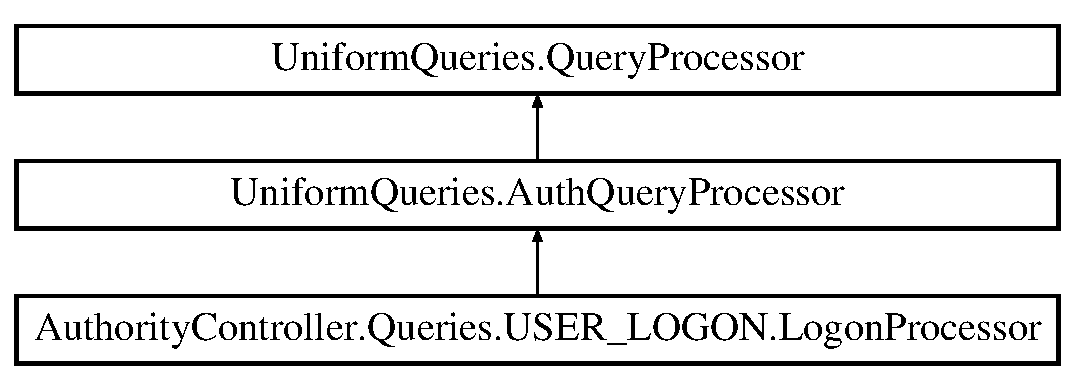
\includegraphics[height=3.000000cm]{db/d30/class_authority_controller_1_1_queries_1_1_u_s_e_r___l_o_g_o_n_1_1_logon_processor}
\end{center}
\end{figure}
\subsection*{Public Member Functions}
\begin{DoxyCompactItemize}
\item 
async void \mbox{\hyperlink{class_authority_controller_1_1_queries_1_1_u_s_e_r___l_o_g_o_n_1_1_logon_processor_a5073849b4aec752f2fb1b68f11561985}{Try\+To\+Logon\+Async}} (string guest\+Token, string login, string password, string server\+IP, string pipe\+Name)
\begin{DoxyCompactList}\small\item\em Logon on routing target server. \end{DoxyCompactList}\end{DoxyCompactItemize}
\subsection*{Additional Inherited Members}


\subsection{Detailed Description}
Handler that provide logogn process. 



\subsection{Member Function Documentation}
\mbox{\Hypertarget{class_authority_controller_1_1_queries_1_1_u_s_e_r___l_o_g_o_n_1_1_logon_processor_a5073849b4aec752f2fb1b68f11561985}\label{class_authority_controller_1_1_queries_1_1_u_s_e_r___l_o_g_o_n_1_1_logon_processor_a5073849b4aec752f2fb1b68f11561985}} 
\index{Authority\+Controller\+::\+Queries\+::\+U\+S\+E\+R\+\_\+\+L\+O\+G\+O\+N\+::\+Logon\+Processor@{Authority\+Controller\+::\+Queries\+::\+U\+S\+E\+R\+\_\+\+L\+O\+G\+O\+N\+::\+Logon\+Processor}!Try\+To\+Logon\+Async@{Try\+To\+Logon\+Async}}
\index{Try\+To\+Logon\+Async@{Try\+To\+Logon\+Async}!Authority\+Controller\+::\+Queries\+::\+U\+S\+E\+R\+\_\+\+L\+O\+G\+O\+N\+::\+Logon\+Processor@{Authority\+Controller\+::\+Queries\+::\+U\+S\+E\+R\+\_\+\+L\+O\+G\+O\+N\+::\+Logon\+Processor}}
\subsubsection{\texorpdfstring{Try\+To\+Logon\+Async()}{TryToLogonAsync()}}
{\footnotesize\ttfamily async void Authority\+Controller.\+Queries.\+U\+S\+E\+R\+\_\+\+L\+O\+G\+O\+N.\+Logon\+Processor.\+Try\+To\+Logon\+Async (\begin{DoxyParamCaption}\item[{string}]{guest\+Token,  }\item[{string}]{login,  }\item[{string}]{password,  }\item[{string}]{server\+IP,  }\item[{string}]{pipe\+Name }\end{DoxyParamCaption})}



Logon on routing target server. 


\begin{DoxyParams}{Parameters}
{\em guest\+Token} & Token that would be able to get guest access on target server.\\
\hline
{\em login} & User\textquotesingle{}s login that would impersonate this server on related server.\\
\hline
{\em password} & User\textquotesingle{}s password.\\
\hline
{\em server\+IP} & IP address of name of server.\\
\hline
{\em pipe\+Name} & Named pipe that started on server.\\
\hline
\end{DoxyParams}


The documentation for this class was generated from the following file\+:\begin{DoxyCompactItemize}
\item 
D\+:/\+Work/\+Git\+Hub/doloro-\/networking-\/framework/\+Addons/\+Authority\+Controller/\+Queries/U\+S\+E\+R\+\_\+\+L\+O\+G\+O\+N.\+cs\end{DoxyCompactItemize}

\hypertarget{struct_pipes_provider_1_1_security_1_1_l_s_a_1_1_lsa_security_wrapper_1_1_l_s_a___o_b_j_e_c_t___a_t_t_r_i_b_u_t_e_s}{}\section{Pipes\+Provider.\+Security.\+L\+S\+A.\+Lsa\+Security\+Wrapper.\+L\+S\+A\+\_\+\+O\+B\+J\+E\+C\+T\+\_\+\+A\+T\+T\+R\+I\+B\+U\+T\+ES Struct Reference}
\label{struct_pipes_provider_1_1_security_1_1_l_s_a_1_1_lsa_security_wrapper_1_1_l_s_a___o_b_j_e_c_t___a_t_t_r_i_b_u_t_e_s}\index{Pipes\+Provider.\+Security.\+L\+S\+A.\+Lsa\+Security\+Wrapper.\+L\+S\+A\+\_\+\+O\+B\+J\+E\+C\+T\+\_\+\+A\+T\+T\+R\+I\+B\+U\+T\+ES@{Pipes\+Provider.\+Security.\+L\+S\+A.\+Lsa\+Security\+Wrapper.\+L\+S\+A\+\_\+\+O\+B\+J\+E\+C\+T\+\_\+\+A\+T\+T\+R\+I\+B\+U\+T\+ES}}
\subsection*{Package Attributes}
\begin{DoxyCompactItemize}
\item 
\mbox{\Hypertarget{struct_pipes_provider_1_1_security_1_1_l_s_a_1_1_lsa_security_wrapper_1_1_l_s_a___o_b_j_e_c_t___a_t_t_r_i_b_u_t_e_s_af6c28e20640088a73ca4fbe164d8fad1}\label{struct_pipes_provider_1_1_security_1_1_l_s_a_1_1_lsa_security_wrapper_1_1_l_s_a___o_b_j_e_c_t___a_t_t_r_i_b_u_t_e_s_af6c28e20640088a73ca4fbe164d8fad1}} 
int {\bfseries Length}
\item 
\mbox{\Hypertarget{struct_pipes_provider_1_1_security_1_1_l_s_a_1_1_lsa_security_wrapper_1_1_l_s_a___o_b_j_e_c_t___a_t_t_r_i_b_u_t_e_s_acf7eb6c79221858596371dd1ddbeb9c9}\label{struct_pipes_provider_1_1_security_1_1_l_s_a_1_1_lsa_security_wrapper_1_1_l_s_a___o_b_j_e_c_t___a_t_t_r_i_b_u_t_e_s_acf7eb6c79221858596371dd1ddbeb9c9}} 
Int\+Ptr {\bfseries Root\+Directory}
\item 
\mbox{\Hypertarget{struct_pipes_provider_1_1_security_1_1_l_s_a_1_1_lsa_security_wrapper_1_1_l_s_a___o_b_j_e_c_t___a_t_t_r_i_b_u_t_e_s_a4911f7b2b4f0cd4121616823bc1ab517}\label{struct_pipes_provider_1_1_security_1_1_l_s_a_1_1_lsa_security_wrapper_1_1_l_s_a___o_b_j_e_c_t___a_t_t_r_i_b_u_t_e_s_a4911f7b2b4f0cd4121616823bc1ab517}} 
Int\+Ptr {\bfseries Object\+Name}
\item 
\mbox{\Hypertarget{struct_pipes_provider_1_1_security_1_1_l_s_a_1_1_lsa_security_wrapper_1_1_l_s_a___o_b_j_e_c_t___a_t_t_r_i_b_u_t_e_s_a206c059deebe7243803b977e29088d5f}\label{struct_pipes_provider_1_1_security_1_1_l_s_a_1_1_lsa_security_wrapper_1_1_l_s_a___o_b_j_e_c_t___a_t_t_r_i_b_u_t_e_s_a206c059deebe7243803b977e29088d5f}} 
int {\bfseries Attributes}
\item 
\mbox{\Hypertarget{struct_pipes_provider_1_1_security_1_1_l_s_a_1_1_lsa_security_wrapper_1_1_l_s_a___o_b_j_e_c_t___a_t_t_r_i_b_u_t_e_s_a8eb1b205242a8c7b72bc804027e03acb}\label{struct_pipes_provider_1_1_security_1_1_l_s_a_1_1_lsa_security_wrapper_1_1_l_s_a___o_b_j_e_c_t___a_t_t_r_i_b_u_t_e_s_a8eb1b205242a8c7b72bc804027e03acb}} 
Int\+Ptr {\bfseries Security\+Descriptor}
\item 
\mbox{\Hypertarget{struct_pipes_provider_1_1_security_1_1_l_s_a_1_1_lsa_security_wrapper_1_1_l_s_a___o_b_j_e_c_t___a_t_t_r_i_b_u_t_e_s_ade6b3f293883f2360deefd4449dffcd8}\label{struct_pipes_provider_1_1_security_1_1_l_s_a_1_1_lsa_security_wrapper_1_1_l_s_a___o_b_j_e_c_t___a_t_t_r_i_b_u_t_e_s_ade6b3f293883f2360deefd4449dffcd8}} 
Int\+Ptr {\bfseries Security\+Quality\+Of\+Service}
\end{DoxyCompactItemize}


The documentation for this struct was generated from the following file\+:\begin{DoxyCompactItemize}
\item 
D\+:/\+Work/\+Git\+Hub/doloro-\/networking-\/framework/\+Core/\+Pipes\+Provider/\+Security/L\+S\+A.\+cs\end{DoxyCompactItemize}

\hypertarget{struct_pipes_provider_1_1_security_1_1_l_s_a_1_1_lsa_security_wrapper_1_1_l_s_a___u_n_i_c_o_d_e___s_t_r_i_n_g}{}\section{Pipes\+Provider.\+Security.\+L\+S\+A.\+Lsa\+Security\+Wrapper.\+L\+S\+A\+\_\+\+U\+N\+I\+C\+O\+D\+E\+\_\+\+S\+T\+R\+I\+NG Struct Reference}
\label{struct_pipes_provider_1_1_security_1_1_l_s_a_1_1_lsa_security_wrapper_1_1_l_s_a___u_n_i_c_o_d_e___s_t_r_i_n_g}\index{Pipes\+Provider.\+Security.\+L\+S\+A.\+Lsa\+Security\+Wrapper.\+L\+S\+A\+\_\+\+U\+N\+I\+C\+O\+D\+E\+\_\+\+S\+T\+R\+I\+NG@{Pipes\+Provider.\+Security.\+L\+S\+A.\+Lsa\+Security\+Wrapper.\+L\+S\+A\+\_\+\+U\+N\+I\+C\+O\+D\+E\+\_\+\+S\+T\+R\+I\+NG}}
\subsection*{Package Attributes}
\begin{DoxyCompactItemize}
\item 
\mbox{\Hypertarget{struct_pipes_provider_1_1_security_1_1_l_s_a_1_1_lsa_security_wrapper_1_1_l_s_a___u_n_i_c_o_d_e___s_t_r_i_n_g_a48ff19f0bbc21f97b2eeb426cc5c3514}\label{struct_pipes_provider_1_1_security_1_1_l_s_a_1_1_lsa_security_wrapper_1_1_l_s_a___u_n_i_c_o_d_e___s_t_r_i_n_g_a48ff19f0bbc21f97b2eeb426cc5c3514}} 
ushort {\bfseries Length}
\item 
\mbox{\Hypertarget{struct_pipes_provider_1_1_security_1_1_l_s_a_1_1_lsa_security_wrapper_1_1_l_s_a___u_n_i_c_o_d_e___s_t_r_i_n_g_a9722e45e60277e9b0b28049783af0ed8}\label{struct_pipes_provider_1_1_security_1_1_l_s_a_1_1_lsa_security_wrapper_1_1_l_s_a___u_n_i_c_o_d_e___s_t_r_i_n_g_a9722e45e60277e9b0b28049783af0ed8}} 
ushort {\bfseries Maximum\+Length}
\item 
\mbox{\Hypertarget{struct_pipes_provider_1_1_security_1_1_l_s_a_1_1_lsa_security_wrapper_1_1_l_s_a___u_n_i_c_o_d_e___s_t_r_i_n_g_a334675cf58725b2410e377674069dbf0}\label{struct_pipes_provider_1_1_security_1_1_l_s_a_1_1_lsa_security_wrapper_1_1_l_s_a___u_n_i_c_o_d_e___s_t_r_i_n_g_a334675cf58725b2410e377674069dbf0}} 
string {\bfseries Buffer}
\end{DoxyCompactItemize}


\subsection{Detailed Description}
\mbox{\hyperlink{struct_pipes_provider_1_1_security_1_1_l_s_a_1_1_lsa_security_wrapper_1_1_l_s_a___u_n_i_c_o_d_e___s_t_r_i_n_g}{L\+S\+A\+\_\+\+U\+N\+I\+C\+O\+D\+E\+\_\+\+S\+T\+R\+I\+NG}} structure 

The documentation for this struct was generated from the following file\+:\begin{DoxyCompactItemize}
\item 
D\+:/\+Work/\+Git\+Hub/doloro-\/networking-\/framework/\+Core/\+Pipes\+Provider/\+Security/L\+S\+A.\+cs\end{DoxyCompactItemize}

\hypertarget{class_pipes_provider_1_1_security_1_1_l_s_a_1_1_lsa_security_wrapper}{}\section{Pipes\+Provider.\+Security.\+L\+S\+A.\+Lsa\+Security\+Wrapper Class Reference}
\label{class_pipes_provider_1_1_security_1_1_l_s_a_1_1_lsa_security_wrapper}\index{Pipes\+Provider.\+Security.\+L\+S\+A.\+Lsa\+Security\+Wrapper@{Pipes\+Provider.\+Security.\+L\+S\+A.\+Lsa\+Security\+Wrapper}}


Provide warped way to Add and Rmove rights for user from \mbox{\hyperlink{namespace_pipes_provider_1_1_security_1_1_l_s_a}{L\+SA}}.  


\subsection*{Static Public Member Functions}
\begin{DoxyCompactItemize}
\item 
static void \mbox{\hyperlink{class_pipes_provider_1_1_security_1_1_l_s_a_1_1_lsa_security_wrapper_adac61a41a0472231a990f1274834ee4d}{Add\+Account\+Rights}} (Security\+Identifier sid, string rights)
\begin{DoxyCompactList}\small\item\em Add rights for requested user or group to \mbox{\hyperlink{namespace_pipes_provider_1_1_security_1_1_l_s_a}{L\+SA}}. \href{https://docs.microsoft.com/en-us/windows/security/threat-protection/security-policy-settings/user-rights-assignment}{\tt https\+://docs.\+microsoft.\+com/en-\/us/windows/security/threat-\/protection/security-\/policy-\/settings/user-\/rights-\/assignment} \end{DoxyCompactList}\item 
static void \mbox{\hyperlink{class_pipes_provider_1_1_security_1_1_l_s_a_1_1_lsa_security_wrapper_ad14aaa2cffa5be534590d0ef30810117}{Remove\+Account\+Rights}} (Security\+Identifier sid, string rights)
\begin{DoxyCompactList}\small\item\em Remove rights for requested user or group from \mbox{\hyperlink{namespace_pipes_provider_1_1_security_1_1_l_s_a}{L\+SA}}. \href{https://docs.microsoft.com/en-us/windows/security/threat-protection/security-policy-settings/user-rights-assignment}{\tt https\+://docs.\+microsoft.\+com/en-\/us/windows/security/threat-\/protection/security-\/policy-\/settings/user-\/rights-\/assignment} \end{DoxyCompactList}\end{DoxyCompactItemize}
\subsection*{Package Functions}
\begin{DoxyCompactItemize}
\item 
\mbox{\Hypertarget{class_pipes_provider_1_1_security_1_1_l_s_a_1_1_lsa_security_wrapper_a773aa7b67cb9fc5616dc6bd1a619b225}\label{class_pipes_provider_1_1_security_1_1_l_s_a_1_1_lsa_security_wrapper_a773aa7b67cb9fc5616dc6bd1a619b225}} 
static uint {\bfseries Lsa\+Open\+Policy} (\mbox{\hyperlink{struct_pipes_provider_1_1_security_1_1_l_s_a_1_1_l_s_a___u_n_i_c_o_d_e___s_t_r_i_n_g}{L\+S\+A\+\_\+\+U\+N\+I\+C\+O\+D\+E\+\_\+\+S\+T\+R\+I\+NG}}\mbox{[}$\,$\mbox{]} System\+Name, ref \mbox{\hyperlink{struct_pipes_provider_1_1_security_1_1_l_s_a_1_1_l_s_a___o_b_j_e_c_t___a_t_t_r_i_b_u_t_e_s}{L\+S\+A\+\_\+\+O\+B\+J\+E\+C\+T\+\_\+\+A\+T\+T\+R\+I\+B\+U\+T\+ES}} Object\+Attributes, int Access\+Mask, out Int\+Ptr Policy\+Handle)
\item 
\mbox{\Hypertarget{class_pipes_provider_1_1_security_1_1_l_s_a_1_1_lsa_security_wrapper_adda333d87687ba6906a623db79a9adfa}\label{class_pipes_provider_1_1_security_1_1_l_s_a_1_1_lsa_security_wrapper_adda333d87687ba6906a623db79a9adfa}} 
static uint {\bfseries Lsa\+Add\+Account\+Rights} (L\+S\+A\+\_\+\+H\+A\+N\+D\+LE Policy\+Handle, Int\+Ptr p\+S\+ID, \mbox{\hyperlink{struct_pipes_provider_1_1_security_1_1_l_s_a_1_1_l_s_a___u_n_i_c_o_d_e___s_t_r_i_n_g}{L\+S\+A\+\_\+\+U\+N\+I\+C\+O\+D\+E\+\_\+\+S\+T\+R\+I\+NG}}\mbox{[}$\,$\mbox{]} User\+Rights, int Count\+Of\+Rights)
\item 
\mbox{\Hypertarget{class_pipes_provider_1_1_security_1_1_l_s_a_1_1_lsa_security_wrapper_adc48b947899763c20b59951bd7d4bf1e}\label{class_pipes_provider_1_1_security_1_1_l_s_a_1_1_lsa_security_wrapper_adc48b947899763c20b59951bd7d4bf1e}} 
static uint {\bfseries Lsa\+Remove\+Account\+Rights} (L\+S\+A\+\_\+\+H\+A\+N\+D\+LE Policy\+Handle, Int\+Ptr Account\+Sid, bool All\+Rights, \mbox{\hyperlink{struct_pipes_provider_1_1_security_1_1_l_s_a_1_1_l_s_a___u_n_i_c_o_d_e___s_t_r_i_n_g}{L\+S\+A\+\_\+\+U\+N\+I\+C\+O\+D\+E\+\_\+\+S\+T\+R\+I\+NG}}\mbox{[}$\,$\mbox{]} User\+Rights, int Count\+Of\+Rights)
\item 
\mbox{\Hypertarget{class_pipes_provider_1_1_security_1_1_l_s_a_1_1_lsa_security_wrapper_a1e3a45dcb55bd6d339ccf426bc600022}\label{class_pipes_provider_1_1_security_1_1_l_s_a_1_1_lsa_security_wrapper_a1e3a45dcb55bd6d339ccf426bc600022}} 
static int {\bfseries Lsa\+Close} (Int\+Ptr Policy\+Handle)
\end{DoxyCompactItemize}
\subsection*{Private Types}
\begin{DoxyCompactItemize}
\item 
\mbox{\Hypertarget{class_pipes_provider_1_1_security_1_1_l_s_a_1_1_lsa_security_wrapper_ac775fcd30d378c71ec29ebe3e8efe778}\label{class_pipes_provider_1_1_security_1_1_l_s_a_1_1_lsa_security_wrapper_ac775fcd30d378c71ec29ebe3e8efe778}} 
enum {\bfseries Access} \+: int \{ {\bfseries P\+O\+L\+I\+C\+Y\+\_\+\+R\+E\+AD} = 0x20006, 
{\bfseries P\+O\+L\+I\+C\+Y\+\_\+\+A\+L\+L\+\_\+\+A\+C\+C\+E\+SS} = 0x00\+F0\+F\+FF, 
{\bfseries P\+O\+L\+I\+C\+Y\+\_\+\+E\+X\+E\+C\+U\+TE} = 0\+X20801, 
{\bfseries P\+O\+L\+I\+C\+Y\+\_\+\+W\+R\+I\+TE} = 0\+X207\+F8
 \}
\end{DoxyCompactItemize}
\subsection*{Static Private Member Functions}
\begin{DoxyCompactItemize}
\item 
static void \mbox{\hyperlink{class_pipes_provider_1_1_security_1_1_l_s_a_1_1_lsa_security_wrapper_a13ce034059c39f7a1a93d06a45b07d94}{Account\+Rights\+Controller}} (Security\+Identifier sid, string rights, bool allow)
\begin{DoxyCompactList}\small\item\em Provide access and overriding of accaunt rights in \mbox{\hyperlink{namespace_pipes_provider_1_1_security_1_1_l_s_a}{L\+SA}}. \end{DoxyCompactList}\end{DoxyCompactItemize}


\subsection{Detailed Description}
Provide warped way to Add and Rmove rights for user from \mbox{\hyperlink{namespace_pipes_provider_1_1_security_1_1_l_s_a}{L\+SA}}. 



\subsection{Member Function Documentation}
\mbox{\Hypertarget{class_pipes_provider_1_1_security_1_1_l_s_a_1_1_lsa_security_wrapper_a13ce034059c39f7a1a93d06a45b07d94}\label{class_pipes_provider_1_1_security_1_1_l_s_a_1_1_lsa_security_wrapper_a13ce034059c39f7a1a93d06a45b07d94}} 
\index{Pipes\+Provider\+::\+Security\+::\+L\+S\+A\+::\+Lsa\+Security\+Wrapper@{Pipes\+Provider\+::\+Security\+::\+L\+S\+A\+::\+Lsa\+Security\+Wrapper}!Account\+Rights\+Controller@{Account\+Rights\+Controller}}
\index{Account\+Rights\+Controller@{Account\+Rights\+Controller}!Pipes\+Provider\+::\+Security\+::\+L\+S\+A\+::\+Lsa\+Security\+Wrapper@{Pipes\+Provider\+::\+Security\+::\+L\+S\+A\+::\+Lsa\+Security\+Wrapper}}
\subsubsection{\texorpdfstring{Account\+Rights\+Controller()}{AccountRightsController()}}
{\footnotesize\ttfamily static void Pipes\+Provider.\+Security.\+L\+S\+A.\+Lsa\+Security\+Wrapper.\+Account\+Rights\+Controller (\begin{DoxyParamCaption}\item[{Security\+Identifier}]{sid,  }\item[{string}]{rights,  }\item[{bool}]{allow }\end{DoxyParamCaption})\hspace{0.3cm}{\ttfamily [static]}, {\ttfamily [private]}}



Provide access and overriding of accaunt rights in \mbox{\hyperlink{namespace_pipes_provider_1_1_security_1_1_l_s_a}{L\+SA}}. 


\begin{DoxyParams}{Parameters}
{\em sid} & \\
\hline
{\em rights} & \\
\hline
{\em allow} & \\
\hline
\end{DoxyParams}
\mbox{\Hypertarget{class_pipes_provider_1_1_security_1_1_l_s_a_1_1_lsa_security_wrapper_adac61a41a0472231a990f1274834ee4d}\label{class_pipes_provider_1_1_security_1_1_l_s_a_1_1_lsa_security_wrapper_adac61a41a0472231a990f1274834ee4d}} 
\index{Pipes\+Provider\+::\+Security\+::\+L\+S\+A\+::\+Lsa\+Security\+Wrapper@{Pipes\+Provider\+::\+Security\+::\+L\+S\+A\+::\+Lsa\+Security\+Wrapper}!Add\+Account\+Rights@{Add\+Account\+Rights}}
\index{Add\+Account\+Rights@{Add\+Account\+Rights}!Pipes\+Provider\+::\+Security\+::\+L\+S\+A\+::\+Lsa\+Security\+Wrapper@{Pipes\+Provider\+::\+Security\+::\+L\+S\+A\+::\+Lsa\+Security\+Wrapper}}
\subsubsection{\texorpdfstring{Add\+Account\+Rights()}{AddAccountRights()}}
{\footnotesize\ttfamily static void Pipes\+Provider.\+Security.\+L\+S\+A.\+Lsa\+Security\+Wrapper.\+Add\+Account\+Rights (\begin{DoxyParamCaption}\item[{Security\+Identifier}]{sid,  }\item[{string}]{rights }\end{DoxyParamCaption})\hspace{0.3cm}{\ttfamily [static]}}



Add rights for requested user or group to \mbox{\hyperlink{namespace_pipes_provider_1_1_security_1_1_l_s_a}{L\+SA}}. \href{https://docs.microsoft.com/en-us/windows/security/threat-protection/security-policy-settings/user-rights-assignment}{\tt https\+://docs.\+microsoft.\+com/en-\/us/windows/security/threat-\/protection/security-\/policy-\/settings/user-\/rights-\/assignment} 


\begin{DoxyParams}{Parameters}
{\em sid} & \\
\hline
{\em rights} & \\
\hline
\end{DoxyParams}
\mbox{\Hypertarget{class_pipes_provider_1_1_security_1_1_l_s_a_1_1_lsa_security_wrapper_ad14aaa2cffa5be534590d0ef30810117}\label{class_pipes_provider_1_1_security_1_1_l_s_a_1_1_lsa_security_wrapper_ad14aaa2cffa5be534590d0ef30810117}} 
\index{Pipes\+Provider\+::\+Security\+::\+L\+S\+A\+::\+Lsa\+Security\+Wrapper@{Pipes\+Provider\+::\+Security\+::\+L\+S\+A\+::\+Lsa\+Security\+Wrapper}!Remove\+Account\+Rights@{Remove\+Account\+Rights}}
\index{Remove\+Account\+Rights@{Remove\+Account\+Rights}!Pipes\+Provider\+::\+Security\+::\+L\+S\+A\+::\+Lsa\+Security\+Wrapper@{Pipes\+Provider\+::\+Security\+::\+L\+S\+A\+::\+Lsa\+Security\+Wrapper}}
\subsubsection{\texorpdfstring{Remove\+Account\+Rights()}{RemoveAccountRights()}}
{\footnotesize\ttfamily static void Pipes\+Provider.\+Security.\+L\+S\+A.\+Lsa\+Security\+Wrapper.\+Remove\+Account\+Rights (\begin{DoxyParamCaption}\item[{Security\+Identifier}]{sid,  }\item[{string}]{rights }\end{DoxyParamCaption})\hspace{0.3cm}{\ttfamily [static]}}



Remove rights for requested user or group from \mbox{\hyperlink{namespace_pipes_provider_1_1_security_1_1_l_s_a}{L\+SA}}. \href{https://docs.microsoft.com/en-us/windows/security/threat-protection/security-policy-settings/user-rights-assignment}{\tt https\+://docs.\+microsoft.\+com/en-\/us/windows/security/threat-\/protection/security-\/policy-\/settings/user-\/rights-\/assignment} 


\begin{DoxyParams}{Parameters}
{\em sid} & \\
\hline
{\em rights} & \\
\hline
\end{DoxyParams}


The documentation for this class was generated from the following file\+:\begin{DoxyCompactItemize}
\item 
D\+:/\+Work/\+Git\+Hub/doloro-\/networking-\/framework/\+Pipes\+Provider/\+Security/L\+S\+A.\+cs\end{DoxyCompactItemize}

\hypertarget{class_pipes_provider_1_1_native_methods}{}\section{Pipes\+Provider.\+Native\+Methods Class Reference}
\label{class_pipes_provider_1_1_native_methods}\index{Pipes\+Provider.\+Native\+Methods@{Pipes\+Provider.\+Native\+Methods}}


Class that provide access to native methods.  


\subsection*{Static Public Member Functions}
\begin{DoxyCompactItemize}
\item 
static bool \mbox{\hyperlink{class_pipes_provider_1_1_native_methods_a9455b60ac124b9a4e3170f1fbbd3c839}{Does\+Named\+Pipe\+Exist}} (string server\+Name, string pipe\+Name)
\begin{DoxyCompactList}\small\item\em Method to test if Windows considers that a named pipe of a certain name exists or not. \end{DoxyCompactList}\end{DoxyCompactItemize}
\subsection*{Private Member Functions}
\begin{DoxyCompactItemize}
\item 
\mbox{\Hypertarget{class_pipes_provider_1_1_native_methods_a1a2952e32dd0e63f65ffd4103eee0942}\label{class_pipes_provider_1_1_native_methods_a1a2952e32dd0e63f65ffd4103eee0942}} 
static bool {\bfseries Wait\+Named\+Pipe} (string name, int timeout)
\end{DoxyCompactItemize}


\subsection{Detailed Description}
Class that provide access to native methods. 



\subsection{Member Function Documentation}
\mbox{\Hypertarget{class_pipes_provider_1_1_native_methods_a9455b60ac124b9a4e3170f1fbbd3c839}\label{class_pipes_provider_1_1_native_methods_a9455b60ac124b9a4e3170f1fbbd3c839}} 
\index{Pipes\+Provider\+::\+Native\+Methods@{Pipes\+Provider\+::\+Native\+Methods}!Does\+Named\+Pipe\+Exist@{Does\+Named\+Pipe\+Exist}}
\index{Does\+Named\+Pipe\+Exist@{Does\+Named\+Pipe\+Exist}!Pipes\+Provider\+::\+Native\+Methods@{Pipes\+Provider\+::\+Native\+Methods}}
\subsubsection{\texorpdfstring{Does\+Named\+Pipe\+Exist()}{DoesNamedPipeExist()}}
{\footnotesize\ttfamily static bool Pipes\+Provider.\+Native\+Methods.\+Does\+Named\+Pipe\+Exist (\begin{DoxyParamCaption}\item[{string}]{server\+Name,  }\item[{string}]{pipe\+Name }\end{DoxyParamCaption})\hspace{0.3cm}{\ttfamily [static]}}



Method to test if Windows considers that a named pipe of a certain name exists or not. 



The documentation for this class was generated from the following file\+:\begin{DoxyCompactItemize}
\item 
D\+:/\+Work/\+Git\+Hub/doloro-\/networking-\/framework/\+Core/\+Pipes\+Provider/Native\+Methods.\+cs\end{DoxyCompactItemize}

\hypertarget{class_pipes_provider_1_1_security_1_1_native_methods}{}\section{Pipes\+Provider.\+Security.\+Native\+Methods Class Reference}
\label{class_pipes_provider_1_1_security_1_1_native_methods}\index{Pipes\+Provider.\+Security.\+Native\+Methods@{Pipes\+Provider.\+Security.\+Native\+Methods}}


Provide access to native metods used in security namespace.  


\subsection*{Public Member Functions}
\begin{DoxyCompactItemize}
\item 
\mbox{\Hypertarget{class_pipes_provider_1_1_security_1_1_native_methods_aa8cbc36f4c83e56734a90e4f82599a14}\label{class_pipes_provider_1_1_security_1_1_native_methods_aa8cbc36f4c83e56734a90e4f82599a14}} 
static bool {\bfseries Logon\+User} (String lpsz\+Username, String lpsz\+Domain, String lpsz\+Password, int dw\+Logon\+Type, int dw\+Logon\+Provider, out Safe\+Access\+Token\+Handle ph\+Token)
\item 
\mbox{\Hypertarget{class_pipes_provider_1_1_security_1_1_native_methods_aaa43d5b08023ba65a847545f43bca37a}\label{class_pipes_provider_1_1_security_1_1_native_methods_aaa43d5b08023ba65a847545f43bca37a}} 
static uint {\bfseries Lsa\+Open\+Policy} (\mbox{\hyperlink{struct_pipes_provider_1_1_security_1_1_l_s_a_1_1_lsa_security_wrapper_1_1_l_s_a___u_n_i_c_o_d_e___s_t_r_i_n_g}{Lsa\+Security\+Wrapper.\+L\+S\+A\+\_\+\+U\+N\+I\+C\+O\+D\+E\+\_\+\+S\+T\+R\+I\+NG}}\mbox{[}$\,$\mbox{]} System\+Name, ref \mbox{\hyperlink{struct_pipes_provider_1_1_security_1_1_l_s_a_1_1_lsa_security_wrapper_1_1_l_s_a___o_b_j_e_c_t___a_t_t_r_i_b_u_t_e_s}{Lsa\+Security\+Wrapper.\+L\+S\+A\+\_\+\+O\+B\+J\+E\+C\+T\+\_\+\+A\+T\+T\+R\+I\+B\+U\+T\+ES}} Object\+Attributes, int Access\+Mask, out Int\+Ptr Policy\+Handle)
\item 
\mbox{\Hypertarget{class_pipes_provider_1_1_security_1_1_native_methods_a41f3c8a115df5b26700d24b6ead2d687}\label{class_pipes_provider_1_1_security_1_1_native_methods_a41f3c8a115df5b26700d24b6ead2d687}} 
static uint {\bfseries Lsa\+Add\+Account\+Rights} (L\+S\+A\+\_\+\+H\+A\+N\+D\+LE Policy\+Handle, Int\+Ptr p\+S\+ID, \mbox{\hyperlink{struct_pipes_provider_1_1_security_1_1_l_s_a_1_1_lsa_security_wrapper_1_1_l_s_a___u_n_i_c_o_d_e___s_t_r_i_n_g}{Lsa\+Security\+Wrapper.\+L\+S\+A\+\_\+\+U\+N\+I\+C\+O\+D\+E\+\_\+\+S\+T\+R\+I\+NG}}\mbox{[}$\,$\mbox{]} User\+Rights, int Count\+Of\+Rights)
\item 
\mbox{\Hypertarget{class_pipes_provider_1_1_security_1_1_native_methods_acf4899aa118ee28b7ea34a51af41a371}\label{class_pipes_provider_1_1_security_1_1_native_methods_acf4899aa118ee28b7ea34a51af41a371}} 
static uint {\bfseries Lsa\+Remove\+Account\+Rights} (L\+S\+A\+\_\+\+H\+A\+N\+D\+LE Policy\+Handle, Int\+Ptr Account\+Sid, bool All\+Rights, \mbox{\hyperlink{struct_pipes_provider_1_1_security_1_1_l_s_a_1_1_lsa_security_wrapper_1_1_l_s_a___u_n_i_c_o_d_e___s_t_r_i_n_g}{Lsa\+Security\+Wrapper.\+L\+S\+A\+\_\+\+U\+N\+I\+C\+O\+D\+E\+\_\+\+S\+T\+R\+I\+NG}}\mbox{[}$\,$\mbox{]} User\+Rights, int Count\+Of\+Rights)
\item 
\mbox{\Hypertarget{class_pipes_provider_1_1_security_1_1_native_methods_ab24dd1a3005b9e4738c8a71b942e682a}\label{class_pipes_provider_1_1_security_1_1_native_methods_ab24dd1a3005b9e4738c8a71b942e682a}} 
static int {\bfseries Lsa\+Close} (Int\+Ptr Policy\+Handle)
\end{DoxyCompactItemize}


\subsection{Detailed Description}
Provide access to native metods used in security namespace. 



The documentation for this class was generated from the following file\+:\begin{DoxyCompactItemize}
\item 
D\+:/\+Work/\+Git\+Hub/doloro-\/networking-\/framework/\+Core/\+Pipes\+Provider/\+Security/Native\+Methods.\+cs\end{DoxyCompactItemize}

\hypertarget{class_uniform_client_1_1_native_methods}{}\section{Uniform\+Client.\+Native\+Methods Class Reference}
\label{class_uniform_client_1_1_native_methods}\index{Uniform\+Client.\+Native\+Methods@{Uniform\+Client.\+Native\+Methods}}
\subsection*{Public Member Functions}
\begin{DoxyCompactItemize}
\item 
static bool \mbox{\hyperlink{class_uniform_client_1_1_native_methods_a067dec2d455070ab352fef3caef7b323}{Show\+Window}} (Int\+Ptr h\+Wnd, int n\+Cmd\+Show)
\begin{DoxyCompactList}\small\item\em Imported method that allo to controll console window state. \end{DoxyCompactList}\item 
static Int\+Ptr \mbox{\hyperlink{class_uniform_client_1_1_native_methods_ab6b4879e450856c501624a55094ead5b}{Get\+Console\+Window}} ()
\begin{DoxyCompactList}\small\item\em Inported method that allow acces to console window. \end{DoxyCompactList}\end{DoxyCompactItemize}


\subsection{Member Function Documentation}
\mbox{\Hypertarget{class_uniform_client_1_1_native_methods_ab6b4879e450856c501624a55094ead5b}\label{class_uniform_client_1_1_native_methods_ab6b4879e450856c501624a55094ead5b}} 
\index{Uniform\+Client\+::\+Native\+Methods@{Uniform\+Client\+::\+Native\+Methods}!Get\+Console\+Window@{Get\+Console\+Window}}
\index{Get\+Console\+Window@{Get\+Console\+Window}!Uniform\+Client\+::\+Native\+Methods@{Uniform\+Client\+::\+Native\+Methods}}
\subsubsection{\texorpdfstring{Get\+Console\+Window()}{GetConsoleWindow()}}
{\footnotesize\ttfamily static Int\+Ptr Uniform\+Client.\+Native\+Methods.\+Get\+Console\+Window (\begin{DoxyParamCaption}{ }\end{DoxyParamCaption})}



Inported method that allow acces to console window. 

\begin{DoxyReturn}{Returns}

\end{DoxyReturn}
\mbox{\Hypertarget{class_uniform_client_1_1_native_methods_a067dec2d455070ab352fef3caef7b323}\label{class_uniform_client_1_1_native_methods_a067dec2d455070ab352fef3caef7b323}} 
\index{Uniform\+Client\+::\+Native\+Methods@{Uniform\+Client\+::\+Native\+Methods}!Show\+Window@{Show\+Window}}
\index{Show\+Window@{Show\+Window}!Uniform\+Client\+::\+Native\+Methods@{Uniform\+Client\+::\+Native\+Methods}}
\subsubsection{\texorpdfstring{Show\+Window()}{ShowWindow()}}
{\footnotesize\ttfamily static bool Uniform\+Client.\+Native\+Methods.\+Show\+Window (\begin{DoxyParamCaption}\item[{Int\+Ptr}]{h\+Wnd,  }\item[{int}]{n\+Cmd\+Show }\end{DoxyParamCaption})}



Imported method that allo to controll console window state. 


\begin{DoxyParams}{Parameters}
{\em h\+Wnd} & \\
\hline
{\em n\+Cmd\+Show} & \\
\hline
\end{DoxyParams}
\begin{DoxyReturn}{Returns}

\end{DoxyReturn}


The documentation for this class was generated from the following file\+:\begin{DoxyCompactItemize}
\item 
D\+:/\+Work/\+Git\+Hub/doloro-\/networking-\/framework/\+Core/\+Uniform\+Client/\+Providers/Native\+Methods.\+cs\end{DoxyCompactItemize}

\hypertarget{class_uniform_server_1_1_native_methods}{}\section{Uniform\+Server.\+Native\+Methods Class Reference}
\label{class_uniform_server_1_1_native_methods}\index{Uniform\+Server.\+Native\+Methods@{Uniform\+Server.\+Native\+Methods}}
\subsection*{Public Member Functions}
\begin{DoxyCompactItemize}
\item 
static bool \mbox{\hyperlink{class_uniform_server_1_1_native_methods_aff29bbaf540e0aebe51ba9fd53576a86}{Show\+Window}} (Int\+Ptr h\+Wnd, int n\+Cmd\+Show)
\begin{DoxyCompactList}\small\item\em Imported method that allo to controll console window state. \end{DoxyCompactList}\item 
static Int\+Ptr \mbox{\hyperlink{class_uniform_server_1_1_native_methods_afe32a1810d024798a409e904c15d1a20}{Get\+Console\+Window}} ()
\begin{DoxyCompactList}\small\item\em Inported method that allow acces to console window. \end{DoxyCompactList}\end{DoxyCompactItemize}


\subsection{Member Function Documentation}
\mbox{\Hypertarget{class_uniform_server_1_1_native_methods_afe32a1810d024798a409e904c15d1a20}\label{class_uniform_server_1_1_native_methods_afe32a1810d024798a409e904c15d1a20}} 
\index{Uniform\+Server\+::\+Native\+Methods@{Uniform\+Server\+::\+Native\+Methods}!Get\+Console\+Window@{Get\+Console\+Window}}
\index{Get\+Console\+Window@{Get\+Console\+Window}!Uniform\+Server\+::\+Native\+Methods@{Uniform\+Server\+::\+Native\+Methods}}
\subsubsection{\texorpdfstring{Get\+Console\+Window()}{GetConsoleWindow()}}
{\footnotesize\ttfamily static Int\+Ptr Uniform\+Server.\+Native\+Methods.\+Get\+Console\+Window (\begin{DoxyParamCaption}{ }\end{DoxyParamCaption})}



Inported method that allow acces to console window. 

\begin{DoxyReturn}{Returns}

\end{DoxyReturn}
\mbox{\Hypertarget{class_uniform_server_1_1_native_methods_aff29bbaf540e0aebe51ba9fd53576a86}\label{class_uniform_server_1_1_native_methods_aff29bbaf540e0aebe51ba9fd53576a86}} 
\index{Uniform\+Server\+::\+Native\+Methods@{Uniform\+Server\+::\+Native\+Methods}!Show\+Window@{Show\+Window}}
\index{Show\+Window@{Show\+Window}!Uniform\+Server\+::\+Native\+Methods@{Uniform\+Server\+::\+Native\+Methods}}
\subsubsection{\texorpdfstring{Show\+Window()}{ShowWindow()}}
{\footnotesize\ttfamily static bool Uniform\+Server.\+Native\+Methods.\+Show\+Window (\begin{DoxyParamCaption}\item[{Int\+Ptr}]{h\+Wnd,  }\item[{int}]{n\+Cmd\+Show }\end{DoxyParamCaption})}



Imported method that allo to controll console window state. 


\begin{DoxyParams}{Parameters}
{\em h\+Wnd} & \\
\hline
{\em n\+Cmd\+Show} & \\
\hline
\end{DoxyParams}
\begin{DoxyReturn}{Returns}

\end{DoxyReturn}


The documentation for this class was generated from the following file\+:\begin{DoxyCompactItemize}
\item 
D\+:/\+Work/\+Git\+Hub/doloro-\/networking-\/framework/\+Core/\+Uniform\+Server/Native\+Methods.\+cs\end{DoxyCompactItemize}

\hypertarget{class_pipes_provider_1_1_networking_1_1_routing_1_1_partial_authorized_instruction}{}\section{Pipes\+Provider.\+Networking.\+Routing.\+Partial\+Authorized\+Instruction Class Reference}
\label{class_pipes_provider_1_1_networking_1_1_routing_1_1_partial_authorized_instruction}\index{Pipes\+Provider.\+Networking.\+Routing.\+Partial\+Authorized\+Instruction@{Pipes\+Provider.\+Networking.\+Routing.\+Partial\+Authorized\+Instruction}}


Provide data and A\+PI required for connections that require partical authorization rights on server.  


Inheritance diagram for Pipes\+Provider.\+Networking.\+Routing.\+Partial\+Authorized\+Instruction\+:\begin{figure}[H]
\begin{center}
\leavevmode
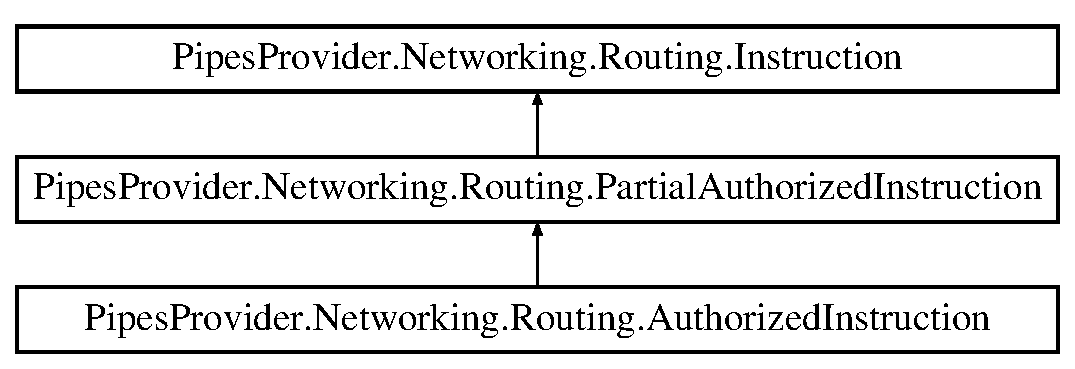
\includegraphics[height=3.000000cm]{dd/df3/class_pipes_provider_1_1_networking_1_1_routing_1_1_partial_authorized_instruction}
\end{center}
\end{figure}
\subsection*{Public Member Functions}
\begin{DoxyCompactItemize}
\item 
async void \mbox{\hyperlink{class_pipes_provider_1_1_networking_1_1_routing_1_1_partial_authorized_instruction_ac84ced39a0d2a20639a82596ef34a093}{Try\+To\+Get\+Guest\+Token\+Async}} (System.\+Action$<$ \mbox{\hyperlink{class_pipes_provider_1_1_networking_1_1_routing_1_1_partial_authorized_instruction}{Partial\+Authorized\+Instruction}} $>$ callback, Cancellation\+Token cancellation\+Token)
\begin{DoxyCompactList}\small\item\em Tring to recive partial authorized token from target server. \end{DoxyCompactList}\item 
bool \mbox{\hyperlink{class_pipes_provider_1_1_networking_1_1_routing_1_1_partial_authorized_instruction_a3ac0a0b15a47f6cfbf26bd0dbabc9b97}{Try\+To\+Get\+Guest\+Token}} (Cancellation\+Token cancellation\+Token)
\begin{DoxyCompactList}\small\item\em Tring to recive partial authorized token from target server. \end{DoxyCompactList}\end{DoxyCompactItemize}
\subsection*{Public Attributes}
\begin{DoxyCompactItemize}
\item 
string \mbox{\hyperlink{class_pipes_provider_1_1_networking_1_1_routing_1_1_partial_authorized_instruction_abda0735bb8ca245802008413dd50c863}{guest\+Chanel}} = \char`\"{}guests\char`\"{}
\begin{DoxyCompactList}\small\item\em Name of the broadcasting pipe that providing guest tokens. \end{DoxyCompactList}\end{DoxyCompactItemize}
\subsection*{Protected Attributes}
\begin{DoxyCompactItemize}
\item 
\mbox{\Hypertarget{class_pipes_provider_1_1_networking_1_1_routing_1_1_partial_authorized_instruction_aef955c1b8751ba406a3b55a7155979c0}\label{class_pipes_provider_1_1_networking_1_1_routing_1_1_partial_authorized_instruction_aef955c1b8751ba406a3b55a7155979c0}} 
\mbox{\hyperlink{class_base_queries_1_1_g_e_t___g_u_e_s_t___t_o_k_e_n_1_1_guest_token_processor}{G\+E\+T\+\_\+\+G\+U\+E\+S\+T\+\_\+\+T\+O\+K\+E\+N.\+Guest\+Token\+Processor}} {\bfseries \+\_\+\+Guest\+Token\+Handler}
\end{DoxyCompactItemize}
\subsection*{Properties}
\begin{DoxyCompactItemize}
\item 
string \mbox{\hyperlink{class_pipes_provider_1_1_networking_1_1_routing_1_1_partial_authorized_instruction_a0818427091144916faf74dab51ac1ba8}{Guest\+Token}}\hspace{0.3cm}{\ttfamily  \mbox{[}get\mbox{]}}
\begin{DoxyCompactList}\small\item\em Return token authorized on target server as guest. \end{DoxyCompactList}\item 
\mbox{\hyperlink{class_base_queries_1_1_g_e_t___g_u_e_s_t___t_o_k_e_n_1_1_guest_token_processor}{G\+E\+T\+\_\+\+G\+U\+E\+S\+T\+\_\+\+T\+O\+K\+E\+N.\+Guest\+Token\+Processor}} \mbox{\hyperlink{class_pipes_provider_1_1_networking_1_1_routing_1_1_partial_authorized_instruction_a2449d0415992bc75cc854859cda8b0bf}{Guest\+Token\+Handler}}\hspace{0.3cm}{\ttfamily  \mbox{[}get\mbox{]}}
\begin{DoxyCompactList}\small\item\em Handler that take full control on reciving of guest token. \end{DoxyCompactList}\end{DoxyCompactItemize}


\subsection{Detailed Description}
Provide data and A\+PI required for connections that require partical authorization rights on server. 



\subsection{Member Function Documentation}
\mbox{\Hypertarget{class_pipes_provider_1_1_networking_1_1_routing_1_1_partial_authorized_instruction_a3ac0a0b15a47f6cfbf26bd0dbabc9b97}\label{class_pipes_provider_1_1_networking_1_1_routing_1_1_partial_authorized_instruction_a3ac0a0b15a47f6cfbf26bd0dbabc9b97}} 
\index{Pipes\+Provider\+::\+Networking\+::\+Routing\+::\+Partial\+Authorized\+Instruction@{Pipes\+Provider\+::\+Networking\+::\+Routing\+::\+Partial\+Authorized\+Instruction}!Try\+To\+Get\+Guest\+Token@{Try\+To\+Get\+Guest\+Token}}
\index{Try\+To\+Get\+Guest\+Token@{Try\+To\+Get\+Guest\+Token}!Pipes\+Provider\+::\+Networking\+::\+Routing\+::\+Partial\+Authorized\+Instruction@{Pipes\+Provider\+::\+Networking\+::\+Routing\+::\+Partial\+Authorized\+Instruction}}
\subsubsection{\texorpdfstring{Try\+To\+Get\+Guest\+Token()}{TryToGetGuestToken()}}
{\footnotesize\ttfamily bool Pipes\+Provider.\+Networking.\+Routing.\+Partial\+Authorized\+Instruction.\+Try\+To\+Get\+Guest\+Token (\begin{DoxyParamCaption}\item[{Cancellation\+Token}]{cancellation\+Token }\end{DoxyParamCaption})}



Tring to recive partial authorized token from target server. 


\begin{DoxyParams}{Parameters}
{\em cancellation\+Token} & Token that can be used to termination of the logon process.\\
\hline
\end{DoxyParams}
\begin{DoxyReturn}{Returns}

\end{DoxyReturn}
\mbox{\Hypertarget{class_pipes_provider_1_1_networking_1_1_routing_1_1_partial_authorized_instruction_ac84ced39a0d2a20639a82596ef34a093}\label{class_pipes_provider_1_1_networking_1_1_routing_1_1_partial_authorized_instruction_ac84ced39a0d2a20639a82596ef34a093}} 
\index{Pipes\+Provider\+::\+Networking\+::\+Routing\+::\+Partial\+Authorized\+Instruction@{Pipes\+Provider\+::\+Networking\+::\+Routing\+::\+Partial\+Authorized\+Instruction}!Try\+To\+Get\+Guest\+Token\+Async@{Try\+To\+Get\+Guest\+Token\+Async}}
\index{Try\+To\+Get\+Guest\+Token\+Async@{Try\+To\+Get\+Guest\+Token\+Async}!Pipes\+Provider\+::\+Networking\+::\+Routing\+::\+Partial\+Authorized\+Instruction@{Pipes\+Provider\+::\+Networking\+::\+Routing\+::\+Partial\+Authorized\+Instruction}}
\subsubsection{\texorpdfstring{Try\+To\+Get\+Guest\+Token\+Async()}{TryToGetGuestTokenAsync()}}
{\footnotesize\ttfamily async void Pipes\+Provider.\+Networking.\+Routing.\+Partial\+Authorized\+Instruction.\+Try\+To\+Get\+Guest\+Token\+Async (\begin{DoxyParamCaption}\item[{System.\+Action$<$ \mbox{\hyperlink{class_pipes_provider_1_1_networking_1_1_routing_1_1_partial_authorized_instruction}{Partial\+Authorized\+Instruction}} $>$}]{callback,  }\item[{Cancellation\+Token}]{cancellation\+Token }\end{DoxyParamCaption})}



Tring to recive partial authorized token from target server. 


\begin{DoxyParams}{Parameters}
{\em callback} & Delegate that will be called when guest token reciving operation would be finished.\\
\hline
{\em cancellation\+Token} & Using this token you can terminate task.\\
\hline
\end{DoxyParams}


\subsection{Member Data Documentation}
\mbox{\Hypertarget{class_pipes_provider_1_1_networking_1_1_routing_1_1_partial_authorized_instruction_abda0735bb8ca245802008413dd50c863}\label{class_pipes_provider_1_1_networking_1_1_routing_1_1_partial_authorized_instruction_abda0735bb8ca245802008413dd50c863}} 
\index{Pipes\+Provider\+::\+Networking\+::\+Routing\+::\+Partial\+Authorized\+Instruction@{Pipes\+Provider\+::\+Networking\+::\+Routing\+::\+Partial\+Authorized\+Instruction}!guest\+Chanel@{guest\+Chanel}}
\index{guest\+Chanel@{guest\+Chanel}!Pipes\+Provider\+::\+Networking\+::\+Routing\+::\+Partial\+Authorized\+Instruction@{Pipes\+Provider\+::\+Networking\+::\+Routing\+::\+Partial\+Authorized\+Instruction}}
\subsubsection{\texorpdfstring{guest\+Chanel}{guestChanel}}
{\footnotesize\ttfamily string Pipes\+Provider.\+Networking.\+Routing.\+Partial\+Authorized\+Instruction.\+guest\+Chanel = \char`\"{}guests\char`\"{}}



Name of the broadcasting pipe that providing guest tokens. 



\subsection{Property Documentation}
\mbox{\Hypertarget{class_pipes_provider_1_1_networking_1_1_routing_1_1_partial_authorized_instruction_a0818427091144916faf74dab51ac1ba8}\label{class_pipes_provider_1_1_networking_1_1_routing_1_1_partial_authorized_instruction_a0818427091144916faf74dab51ac1ba8}} 
\index{Pipes\+Provider\+::\+Networking\+::\+Routing\+::\+Partial\+Authorized\+Instruction@{Pipes\+Provider\+::\+Networking\+::\+Routing\+::\+Partial\+Authorized\+Instruction}!Guest\+Token@{Guest\+Token}}
\index{Guest\+Token@{Guest\+Token}!Pipes\+Provider\+::\+Networking\+::\+Routing\+::\+Partial\+Authorized\+Instruction@{Pipes\+Provider\+::\+Networking\+::\+Routing\+::\+Partial\+Authorized\+Instruction}}
\subsubsection{\texorpdfstring{Guest\+Token}{GuestToken}}
{\footnotesize\ttfamily string Pipes\+Provider.\+Networking.\+Routing.\+Partial\+Authorized\+Instruction.\+Guest\+Token\hspace{0.3cm}{\ttfamily [get]}}



Return token authorized on target server as guest. 

\mbox{\Hypertarget{class_pipes_provider_1_1_networking_1_1_routing_1_1_partial_authorized_instruction_a2449d0415992bc75cc854859cda8b0bf}\label{class_pipes_provider_1_1_networking_1_1_routing_1_1_partial_authorized_instruction_a2449d0415992bc75cc854859cda8b0bf}} 
\index{Pipes\+Provider\+::\+Networking\+::\+Routing\+::\+Partial\+Authorized\+Instruction@{Pipes\+Provider\+::\+Networking\+::\+Routing\+::\+Partial\+Authorized\+Instruction}!Guest\+Token\+Handler@{Guest\+Token\+Handler}}
\index{Guest\+Token\+Handler@{Guest\+Token\+Handler}!Pipes\+Provider\+::\+Networking\+::\+Routing\+::\+Partial\+Authorized\+Instruction@{Pipes\+Provider\+::\+Networking\+::\+Routing\+::\+Partial\+Authorized\+Instruction}}
\subsubsection{\texorpdfstring{Guest\+Token\+Handler}{GuestTokenHandler}}
{\footnotesize\ttfamily \mbox{\hyperlink{class_base_queries_1_1_g_e_t___g_u_e_s_t___t_o_k_e_n_1_1_guest_token_processor}{G\+E\+T\+\_\+\+G\+U\+E\+S\+T\+\_\+\+T\+O\+K\+E\+N.\+Guest\+Token\+Processor}} Pipes\+Provider.\+Networking.\+Routing.\+Partial\+Authorized\+Instruction.\+Guest\+Token\+Handler\hspace{0.3cm}{\ttfamily [get]}}



Handler that take full control on reciving of guest token. 



The documentation for this class was generated from the following file\+:\begin{DoxyCompactItemize}
\item 
D\+:/\+Work/\+Git\+Hub/doloro-\/networking-\/framework/\+Core/\+D\+N\+F\+Core/\+Uniform\+Client/\+Extensions/\+Pipes\+Provider/Partial\+Authorized\+Instruction.\+cs\end{DoxyCompactItemize}

\hypertarget{class_pipes_provider_1_1_handlers_1_1_query}{}\section{Pipes\+Provider.\+Handlers.\+Query Class Reference}
\label{class_pipes_provider_1_1_handlers_1_1_query}\index{Pipes\+Provider.\+Handlers.\+Query@{Pipes\+Provider.\+Handlers.\+Query}}
\subsection*{Static Public Member Functions}
\begin{DoxyCompactItemize}
\item 
static async void \mbox{\hyperlink{class_pipes_provider_1_1_handlers_1_1_query_a3f08c44bfaf5e720d6dfbd791227c8fe}{Processing\+Async}} (\mbox{\hyperlink{class_pipes_provider_1_1_server_1_1_transmission_controllers_1_1_base_server_transmission_controller}{Base\+Server\+Transmission\+Controller}} \+\_\+, string query)
\begin{DoxyCompactList}\small\item\em Handler that can be connected as callback to default Pipes\+Provides \mbox{\hyperlink{class_pipes_provider_1_1_handlers_1_1_d_n_s}{D\+NS}} Handler. Will validate and decompose querie on parts and send it to target Query\+Processor. \end{DoxyCompactList}\end{DoxyCompactItemize}


\subsection{Member Function Documentation}
\mbox{\Hypertarget{class_pipes_provider_1_1_handlers_1_1_query_a3f08c44bfaf5e720d6dfbd791227c8fe}\label{class_pipes_provider_1_1_handlers_1_1_query_a3f08c44bfaf5e720d6dfbd791227c8fe}} 
\index{Pipes\+Provider\+::\+Handlers\+::\+Query@{Pipes\+Provider\+::\+Handlers\+::\+Query}!Processing\+Async@{Processing\+Async}}
\index{Processing\+Async@{Processing\+Async}!Pipes\+Provider\+::\+Handlers\+::\+Query@{Pipes\+Provider\+::\+Handlers\+::\+Query}}
\subsubsection{\texorpdfstring{Processing\+Async()}{ProcessingAsync()}}
{\footnotesize\ttfamily static async void Pipes\+Provider.\+Handlers.\+Query.\+Processing\+Async (\begin{DoxyParamCaption}\item[{\mbox{\hyperlink{class_pipes_provider_1_1_server_1_1_transmission_controllers_1_1_base_server_transmission_controller}{Base\+Server\+Transmission\+Controller}}}]{\+\_\+,  }\item[{string}]{query }\end{DoxyParamCaption})\hspace{0.3cm}{\ttfamily [static]}}



Handler that can be connected as callback to default Pipes\+Provides \mbox{\hyperlink{class_pipes_provider_1_1_handlers_1_1_d_n_s}{D\+NS}} Handler. Will validate and decompose querie on parts and send it to target Query\+Processor. 


\begin{DoxyParams}{Parameters}
{\em meta} & \\
\hline
{\em query} & \\
\hline
\end{DoxyParams}


The documentation for this class was generated from the following file\+:\begin{DoxyCompactItemize}
\item 
D\+:/\+Work/\+Git\+Hub/doloro-\/networking-\/framework/\+Core/\+Pipes\+Provider/\+Handlers/Query.\+cs\end{DoxyCompactItemize}

\hypertarget{struct_pipes_provider_1_1_client_1_1_query_container}{}\section{Pipes\+Provider.\+Client.\+Query\+Container Struct Reference}
\label{struct_pipes_provider_1_1_client_1_1_query_container}\index{Pipes\+Provider.\+Client.\+Query\+Container@{Pipes\+Provider.\+Client.\+Query\+Container}}


Privide invormation about query.  


\subsection*{Public Member Functions}
\begin{DoxyCompactItemize}
\item 
\mbox{\hyperlink{struct_pipes_provider_1_1_client_1_1_query_container_a35009271933f6aebf60be2415b651067}{Query\+Container}} (string query)
\begin{DoxyCompactList}\small\item\em Constructor that provide single way query. \end{DoxyCompactList}\item 
\mbox{\hyperlink{struct_pipes_provider_1_1_client_1_1_query_container_a0e78a9dc3d3fc971f9a1abb06dc836b4}{Query\+Container}} (string query, System.\+Action$<$ \mbox{\hyperlink{class_pipes_provider_1_1_client_1_1_transmission_line}{Transmission\+Line}}, string $>$ \mbox{\hyperlink{struct_pipes_provider_1_1_client_1_1_query_container_acaaa09658d3bb75118670fbb90b77f33}{Answer\+Handler}})
\begin{DoxyCompactList}\small\item\em Constructor of contaier that provide ability to create duplex query. \end{DoxyCompactList}\item 
\mbox{\Hypertarget{struct_pipes_provider_1_1_client_1_1_query_container_a567d4d144909e8e480c30f1faacadbc3}\label{struct_pipes_provider_1_1_client_1_1_query_container_a567d4d144909e8e480c30f1faacadbc3}} 
override string {\bfseries To\+String} ()
\end{DoxyCompactItemize}
\subsection*{Static Public Member Functions}
\begin{DoxyCompactItemize}
\item 
static \mbox{\hyperlink{struct_pipes_provider_1_1_client_1_1_query_container}{Query\+Container}} \mbox{\hyperlink{struct_pipes_provider_1_1_client_1_1_query_container_acfcd11bf7f6b6c9cc4e6b2ff574437bd}{Copy}} (\mbox{\hyperlink{struct_pipes_provider_1_1_client_1_1_query_container}{Query\+Container}} source)
\begin{DoxyCompactList}\small\item\em Return copy of source container. \end{DoxyCompactList}\item 
static \mbox{\hyperlink{struct_pipes_provider_1_1_client_1_1_query_container}{Query\+Container}} \mbox{\hyperlink{struct_pipes_provider_1_1_client_1_1_query_container_a9a97cf832c6736f14f5ed2661fbb3bce}{operator++}} (\mbox{\hyperlink{struct_pipes_provider_1_1_client_1_1_query_container}{Query\+Container}} contaier)
\begin{DoxyCompactList}\small\item\em Incremet of attempts count. \end{DoxyCompactList}\item 
static \mbox{\hyperlink{struct_pipes_provider_1_1_client_1_1_query_container_a0d227c39b9ecec5d8b3e739e87e171a6}{operator string}} (\mbox{\hyperlink{struct_pipes_provider_1_1_client_1_1_query_container}{Query\+Container}} container)
\begin{DoxyCompactList}\small\item\em Convert container to string. \end{DoxyCompactList}\end{DoxyCompactItemize}
\subsection*{Public Attributes}
\begin{DoxyCompactItemize}
\item 
System.\+Action$<$ \mbox{\hyperlink{class_pipes_provider_1_1_client_1_1_transmission_line}{Transmission\+Line}}, string $>$ \mbox{\hyperlink{struct_pipes_provider_1_1_client_1_1_query_container_acaaa09658d3bb75118670fbb90b77f33}{Answer\+Handler}}
\begin{DoxyCompactList}\small\item\em Delegate that will be called when anser transmition will be recived. \end{DoxyCompactList}\end{DoxyCompactItemize}
\subsection*{Properties}
\begin{DoxyCompactItemize}
\item 
string \mbox{\hyperlink{struct_pipes_provider_1_1_client_1_1_query_container_ada0fa04c68e6aee41d3d811d699d01aa}{Query}}\hspace{0.3cm}{\ttfamily  \mbox{[}get, set\mbox{]}}
\begin{DoxyCompactList}\small\item\em Query that will be shared. \end{DoxyCompactList}\item 
bool \mbox{\hyperlink{struct_pipes_provider_1_1_client_1_1_query_container_ab2ceeaac61f04d4ce7e41bc8ea931a0f}{Is\+Empty}}\hspace{0.3cm}{\ttfamily  \mbox{[}get\mbox{]}}
\begin{DoxyCompactList}\small\item\em Validate container. \end{DoxyCompactList}\item 
int \mbox{\hyperlink{struct_pipes_provider_1_1_client_1_1_query_container_a565336905463066277e39b0dbe606112}{Attempts}}\hspace{0.3cm}{\ttfamily  \mbox{[}get, private set\mbox{]}}
\begin{DoxyCompactList}\small\item\em How many attemts was applied to this query processing. \end{DoxyCompactList}\item 
static \mbox{\hyperlink{struct_pipes_provider_1_1_client_1_1_query_container}{Query\+Container}} \mbox{\hyperlink{struct_pipes_provider_1_1_client_1_1_query_container_a0e1f91d0a990824b56170c3da5e5919c}{Empty}} = new \mbox{\hyperlink{struct_pipes_provider_1_1_client_1_1_query_container}{Query\+Container}}()\hspace{0.3cm}{\ttfamily  \mbox{[}get\mbox{]}}
\begin{DoxyCompactList}\small\item\em Return empty contaier. \end{DoxyCompactList}\end{DoxyCompactItemize}


\subsection{Detailed Description}
Privide invormation about query. 



\subsection{Constructor \& Destructor Documentation}
\mbox{\Hypertarget{struct_pipes_provider_1_1_client_1_1_query_container_a35009271933f6aebf60be2415b651067}\label{struct_pipes_provider_1_1_client_1_1_query_container_a35009271933f6aebf60be2415b651067}} 
\index{Pipes\+Provider\+::\+Client\+::\+Query\+Container@{Pipes\+Provider\+::\+Client\+::\+Query\+Container}!Query\+Container@{Query\+Container}}
\index{Query\+Container@{Query\+Container}!Pipes\+Provider\+::\+Client\+::\+Query\+Container@{Pipes\+Provider\+::\+Client\+::\+Query\+Container}}
\subsubsection{\texorpdfstring{Query\+Container()}{QueryContainer()}\hspace{0.1cm}{\footnotesize\ttfamily [1/2]}}
{\footnotesize\ttfamily Pipes\+Provider.\+Client.\+Query\+Container.\+Query\+Container (\begin{DoxyParamCaption}\item[{string}]{query }\end{DoxyParamCaption})}



Constructor that provide single way query. 


\begin{DoxyParams}{Parameters}
{\em query} & \\
\hline
\end{DoxyParams}
\mbox{\Hypertarget{struct_pipes_provider_1_1_client_1_1_query_container_a0e78a9dc3d3fc971f9a1abb06dc836b4}\label{struct_pipes_provider_1_1_client_1_1_query_container_a0e78a9dc3d3fc971f9a1abb06dc836b4}} 
\index{Pipes\+Provider\+::\+Client\+::\+Query\+Container@{Pipes\+Provider\+::\+Client\+::\+Query\+Container}!Query\+Container@{Query\+Container}}
\index{Query\+Container@{Query\+Container}!Pipes\+Provider\+::\+Client\+::\+Query\+Container@{Pipes\+Provider\+::\+Client\+::\+Query\+Container}}
\subsubsection{\texorpdfstring{Query\+Container()}{QueryContainer()}\hspace{0.1cm}{\footnotesize\ttfamily [2/2]}}
{\footnotesize\ttfamily Pipes\+Provider.\+Client.\+Query\+Container.\+Query\+Container (\begin{DoxyParamCaption}\item[{string}]{query,  }\item[{System.\+Action$<$ \mbox{\hyperlink{class_pipes_provider_1_1_client_1_1_transmission_line}{Transmission\+Line}}, string $>$}]{Answer\+Handler }\end{DoxyParamCaption})}



Constructor of contaier that provide ability to create duplex query. 


\begin{DoxyParams}{Parameters}
{\em query} & \\
\hline
{\em Answer\+Handler} & \\
\hline
\end{DoxyParams}


\subsection{Member Function Documentation}
\mbox{\Hypertarget{struct_pipes_provider_1_1_client_1_1_query_container_acfcd11bf7f6b6c9cc4e6b2ff574437bd}\label{struct_pipes_provider_1_1_client_1_1_query_container_acfcd11bf7f6b6c9cc4e6b2ff574437bd}} 
\index{Pipes\+Provider\+::\+Client\+::\+Query\+Container@{Pipes\+Provider\+::\+Client\+::\+Query\+Container}!Copy@{Copy}}
\index{Copy@{Copy}!Pipes\+Provider\+::\+Client\+::\+Query\+Container@{Pipes\+Provider\+::\+Client\+::\+Query\+Container}}
\subsubsection{\texorpdfstring{Copy()}{Copy()}}
{\footnotesize\ttfamily static \mbox{\hyperlink{struct_pipes_provider_1_1_client_1_1_query_container}{Query\+Container}} Pipes\+Provider.\+Client.\+Query\+Container.\+Copy (\begin{DoxyParamCaption}\item[{\mbox{\hyperlink{struct_pipes_provider_1_1_client_1_1_query_container}{Query\+Container}}}]{source }\end{DoxyParamCaption})\hspace{0.3cm}{\ttfamily [static]}}



Return copy of source container. 


\begin{DoxyParams}{Parameters}
{\em source} & \\
\hline
\end{DoxyParams}
\begin{DoxyReturn}{Returns}

\end{DoxyReturn}
\mbox{\Hypertarget{struct_pipes_provider_1_1_client_1_1_query_container_a0d227c39b9ecec5d8b3e739e87e171a6}\label{struct_pipes_provider_1_1_client_1_1_query_container_a0d227c39b9ecec5d8b3e739e87e171a6}} 
\index{Pipes\+Provider\+::\+Client\+::\+Query\+Container@{Pipes\+Provider\+::\+Client\+::\+Query\+Container}!operator string@{operator string}}
\index{operator string@{operator string}!Pipes\+Provider\+::\+Client\+::\+Query\+Container@{Pipes\+Provider\+::\+Client\+::\+Query\+Container}}
\subsubsection{\texorpdfstring{operator string()}{operator string()}}
{\footnotesize\ttfamily static Pipes\+Provider.\+Client.\+Query\+Container.\+operator string (\begin{DoxyParamCaption}\item[{\mbox{\hyperlink{struct_pipes_provider_1_1_client_1_1_query_container}{Query\+Container}}}]{container }\end{DoxyParamCaption})\hspace{0.3cm}{\ttfamily [explicit]}, {\ttfamily [static]}}



Convert container to string. 


\begin{DoxyParams}{Parameters}
{\em container} & \\
\hline
\end{DoxyParams}
\mbox{\Hypertarget{struct_pipes_provider_1_1_client_1_1_query_container_a9a97cf832c6736f14f5ed2661fbb3bce}\label{struct_pipes_provider_1_1_client_1_1_query_container_a9a97cf832c6736f14f5ed2661fbb3bce}} 
\index{Pipes\+Provider\+::\+Client\+::\+Query\+Container@{Pipes\+Provider\+::\+Client\+::\+Query\+Container}!operator++@{operator++}}
\index{operator++@{operator++}!Pipes\+Provider\+::\+Client\+::\+Query\+Container@{Pipes\+Provider\+::\+Client\+::\+Query\+Container}}
\subsubsection{\texorpdfstring{operator++()}{operator++()}}
{\footnotesize\ttfamily static \mbox{\hyperlink{struct_pipes_provider_1_1_client_1_1_query_container}{Query\+Container}} Pipes\+Provider.\+Client.\+Query\+Container.\+operator++ (\begin{DoxyParamCaption}\item[{\mbox{\hyperlink{struct_pipes_provider_1_1_client_1_1_query_container}{Query\+Container}}}]{contaier }\end{DoxyParamCaption})\hspace{0.3cm}{\ttfamily [static]}}



Incremet of attempts count. 


\begin{DoxyParams}{Parameters}
{\em contaier} & \\
\hline
\end{DoxyParams}
\begin{DoxyReturn}{Returns}

\end{DoxyReturn}


\subsection{Member Data Documentation}
\mbox{\Hypertarget{struct_pipes_provider_1_1_client_1_1_query_container_acaaa09658d3bb75118670fbb90b77f33}\label{struct_pipes_provider_1_1_client_1_1_query_container_acaaa09658d3bb75118670fbb90b77f33}} 
\index{Pipes\+Provider\+::\+Client\+::\+Query\+Container@{Pipes\+Provider\+::\+Client\+::\+Query\+Container}!Answer\+Handler@{Answer\+Handler}}
\index{Answer\+Handler@{Answer\+Handler}!Pipes\+Provider\+::\+Client\+::\+Query\+Container@{Pipes\+Provider\+::\+Client\+::\+Query\+Container}}
\subsubsection{\texorpdfstring{Answer\+Handler}{AnswerHandler}}
{\footnotesize\ttfamily System.\+Action$<$\mbox{\hyperlink{class_pipes_provider_1_1_client_1_1_transmission_line}{Transmission\+Line}}, string$>$ Pipes\+Provider.\+Client.\+Query\+Container.\+Answer\+Handler}



Delegate that will be called when anser transmition will be recived. 



\subsection{Property Documentation}
\mbox{\Hypertarget{struct_pipes_provider_1_1_client_1_1_query_container_a565336905463066277e39b0dbe606112}\label{struct_pipes_provider_1_1_client_1_1_query_container_a565336905463066277e39b0dbe606112}} 
\index{Pipes\+Provider\+::\+Client\+::\+Query\+Container@{Pipes\+Provider\+::\+Client\+::\+Query\+Container}!Attempts@{Attempts}}
\index{Attempts@{Attempts}!Pipes\+Provider\+::\+Client\+::\+Query\+Container@{Pipes\+Provider\+::\+Client\+::\+Query\+Container}}
\subsubsection{\texorpdfstring{Attempts}{Attempts}}
{\footnotesize\ttfamily int Pipes\+Provider.\+Client.\+Query\+Container.\+Attempts\hspace{0.3cm}{\ttfamily [get]}, {\ttfamily [private set]}}



How many attemts was applied to this query processing. 

\mbox{\Hypertarget{struct_pipes_provider_1_1_client_1_1_query_container_a0e1f91d0a990824b56170c3da5e5919c}\label{struct_pipes_provider_1_1_client_1_1_query_container_a0e1f91d0a990824b56170c3da5e5919c}} 
\index{Pipes\+Provider\+::\+Client\+::\+Query\+Container@{Pipes\+Provider\+::\+Client\+::\+Query\+Container}!Empty@{Empty}}
\index{Empty@{Empty}!Pipes\+Provider\+::\+Client\+::\+Query\+Container@{Pipes\+Provider\+::\+Client\+::\+Query\+Container}}
\subsubsection{\texorpdfstring{Empty}{Empty}}
{\footnotesize\ttfamily \mbox{\hyperlink{struct_pipes_provider_1_1_client_1_1_query_container}{Query\+Container}} Pipes\+Provider.\+Client.\+Query\+Container.\+Empty = new \mbox{\hyperlink{struct_pipes_provider_1_1_client_1_1_query_container}{Query\+Container}}()\hspace{0.3cm}{\ttfamily [static]}, {\ttfamily [get]}}



Return empty contaier. 

\mbox{\Hypertarget{struct_pipes_provider_1_1_client_1_1_query_container_ab2ceeaac61f04d4ce7e41bc8ea931a0f}\label{struct_pipes_provider_1_1_client_1_1_query_container_ab2ceeaac61f04d4ce7e41bc8ea931a0f}} 
\index{Pipes\+Provider\+::\+Client\+::\+Query\+Container@{Pipes\+Provider\+::\+Client\+::\+Query\+Container}!Is\+Empty@{Is\+Empty}}
\index{Is\+Empty@{Is\+Empty}!Pipes\+Provider\+::\+Client\+::\+Query\+Container@{Pipes\+Provider\+::\+Client\+::\+Query\+Container}}
\subsubsection{\texorpdfstring{Is\+Empty}{IsEmpty}}
{\footnotesize\ttfamily bool Pipes\+Provider.\+Client.\+Query\+Container.\+Is\+Empty\hspace{0.3cm}{\ttfamily [get]}}



Validate container. 

\mbox{\Hypertarget{struct_pipes_provider_1_1_client_1_1_query_container_ada0fa04c68e6aee41d3d811d699d01aa}\label{struct_pipes_provider_1_1_client_1_1_query_container_ada0fa04c68e6aee41d3d811d699d01aa}} 
\index{Pipes\+Provider\+::\+Client\+::\+Query\+Container@{Pipes\+Provider\+::\+Client\+::\+Query\+Container}!Query@{Query}}
\index{Query@{Query}!Pipes\+Provider\+::\+Client\+::\+Query\+Container@{Pipes\+Provider\+::\+Client\+::\+Query\+Container}}
\subsubsection{\texorpdfstring{Query}{Query}}
{\footnotesize\ttfamily string Pipes\+Provider.\+Client.\+Query\+Container.\+Query\hspace{0.3cm}{\ttfamily [get]}, {\ttfamily [set]}}



Query that will be shared. 



The documentation for this struct was generated from the following file\+:\begin{DoxyCompactItemize}
\item 
D\+:/\+Work/\+Git\+Hub/doloro-\/networking-\/framework/\+Pipes\+Provider/\+Server/Query\+Container.\+cs\end{DoxyCompactItemize}

\hypertarget{struct_uniform_queries_1_1_query_part}{}\section{Uniform\+Queries.\+Query\+Part Struct Reference}
\label{struct_uniform_queries_1_1_query_part}\index{Uniform\+Queries.\+Query\+Part@{Uniform\+Queries.\+Query\+Part}}
\subsection*{Public Member Functions}
\begin{DoxyCompactItemize}
\item 
\mbox{\hyperlink{struct_uniform_queries_1_1_query_part_ae8a918635c52a837300ff3b1fdcdfd57}{Query\+Part}} (string key)
\begin{DoxyCompactList}\small\item\em Base constructor. Value will be null \end{DoxyCompactList}\item 
\mbox{\hyperlink{struct_uniform_queries_1_1_query_part_adabbcaa15ccf653f686d4f2bcd39ce09}{Query\+Part}} (string key, string property)
\begin{DoxyCompactList}\small\item\em Base constructor. \end{DoxyCompactList}\item 
override string \mbox{\hyperlink{struct_uniform_queries_1_1_query_part_acf5597530f693df3804fc2e638805245}{To\+String}} ()
\begin{DoxyCompactList}\small\item\em Return part in query format. \end{DoxyCompactList}\item 
bool \mbox{\hyperlink{struct_uniform_queries_1_1_query_part_af032469107805c1c71083666bb8548a9}{Param\+Name\+Equal}} (string key)
\begin{DoxyCompactList}\small\item\em Check does this query\textquotesingle{}s key equals to target. \end{DoxyCompactList}\item 
bool \mbox{\hyperlink{struct_uniform_queries_1_1_query_part_a5fb4475a72dcb6882fc860f7c0fcc50e}{Param\+Value\+Equal}} (string param)
\begin{DoxyCompactList}\small\item\em Check does this query\textquotesingle{}s parameter equals to target. \end{DoxyCompactList}\end{DoxyCompactItemize}
\subsection*{Static Public Member Functions}
\begin{DoxyCompactItemize}
\item 
static implicit \mbox{\hyperlink{struct_uniform_queries_1_1_query_part_a274b321f91ecbda08f01c23536a568b6}{operator string}} (\mbox{\hyperlink{struct_uniform_queries_1_1_query_part}{Query\+Part}} qp)
\begin{DoxyCompactList}\small\item\em Convert \mbox{\hyperlink{struct_uniform_queries_1_1_query_part}{Query\+Part}} to string. \end{DoxyCompactList}\item 
static \mbox{\hyperlink{struct_uniform_queries_1_1_query_part_ab0c6ca9b91045a64286bf730ad97dc43}{operator Query\+Part}} (string builded\+Part)
\begin{DoxyCompactList}\small\item\em Convert string to Qury Part. \end{DoxyCompactList}\item 
static string \mbox{\hyperlink{struct_uniform_queries_1_1_query_part_a053c8ba08ddd1a20d5b50128a524da09}{Query\+Parts\+Array\+To\+String}} (\mbox{\hyperlink{struct_uniform_queries_1_1_query_part}{Query\+Part}}\mbox{[}$\,$\mbox{]} query\+Parts)
\begin{DoxyCompactList}\small\item\em Convert array to query string. \end{DoxyCompactList}\item 
static bool \mbox{\hyperlink{struct_uniform_queries_1_1_query_part_accd3b435809c426dd92456ffee0a996d}{Try\+Get\+Backward\+Domain}} (\mbox{\hyperlink{struct_uniform_queries_1_1_query_part}{Query\+Part}}\mbox{[}$\,$\mbox{]} query\+Parts, out string domain)
\begin{DoxyCompactList}\small\item\em Try to get domain to backward connection by entry query. \end{DoxyCompactList}\end{DoxyCompactItemize}
\subsection*{Public Attributes}
\begin{DoxyCompactItemize}
\item 
string \mbox{\hyperlink{struct_uniform_queries_1_1_query_part_a941540a3d1489c7f32cb5e21910ba7ac}{property\+Name}}
\begin{DoxyCompactList}\small\item\em Key for access \end{DoxyCompactList}\item 
string \mbox{\hyperlink{struct_uniform_queries_1_1_query_part_adb297c368ab4900f751d60ceffda0a99}{property\+Value}}
\begin{DoxyCompactList}\small\item\em Property that will be shared via query. \end{DoxyCompactList}\end{DoxyCompactItemize}
\subsection*{Properties}
\begin{DoxyCompactItemize}
\item 
bool \mbox{\hyperlink{struct_uniform_queries_1_1_query_part_af380375ca82e9dc2eecf899b5933fe2b}{Is\+None}}\hspace{0.3cm}{\ttfamily  \mbox{[}get\mbox{]}}
\begin{DoxyCompactList}\small\item\em If this struct not initialized. \end{DoxyCompactList}\item 
\mbox{\Hypertarget{struct_uniform_queries_1_1_query_part_a5be54faa8b7723167257e930a71457a4}\label{struct_uniform_queries_1_1_query_part_a5be54faa8b7723167257e930a71457a4}} 
static \mbox{\hyperlink{struct_uniform_queries_1_1_query_part}{Query\+Part}} {\bfseries None}\hspace{0.3cm}{\ttfamily  \mbox{[}get\mbox{]}}
\end{DoxyCompactItemize}


\subsection{Constructor \& Destructor Documentation}
\mbox{\Hypertarget{struct_uniform_queries_1_1_query_part_ae8a918635c52a837300ff3b1fdcdfd57}\label{struct_uniform_queries_1_1_query_part_ae8a918635c52a837300ff3b1fdcdfd57}} 
\index{Uniform\+Queries\+::\+Query\+Part@{Uniform\+Queries\+::\+Query\+Part}!Query\+Part@{Query\+Part}}
\index{Query\+Part@{Query\+Part}!Uniform\+Queries\+::\+Query\+Part@{Uniform\+Queries\+::\+Query\+Part}}
\subsubsection{\texorpdfstring{Query\+Part()}{QueryPart()}\hspace{0.1cm}{\footnotesize\ttfamily [1/2]}}
{\footnotesize\ttfamily Uniform\+Queries.\+Query\+Part.\+Query\+Part (\begin{DoxyParamCaption}\item[{string}]{key }\end{DoxyParamCaption})}



Base constructor. Value will be null 


\begin{DoxyParams}{Parameters}
{\em key} & String key that allow to find this part in query.\\
\hline
\end{DoxyParams}
\mbox{\Hypertarget{struct_uniform_queries_1_1_query_part_adabbcaa15ccf653f686d4f2bcd39ce09}\label{struct_uniform_queries_1_1_query_part_adabbcaa15ccf653f686d4f2bcd39ce09}} 
\index{Uniform\+Queries\+::\+Query\+Part@{Uniform\+Queries\+::\+Query\+Part}!Query\+Part@{Query\+Part}}
\index{Query\+Part@{Query\+Part}!Uniform\+Queries\+::\+Query\+Part@{Uniform\+Queries\+::\+Query\+Part}}
\subsubsection{\texorpdfstring{Query\+Part()}{QueryPart()}\hspace{0.1cm}{\footnotesize\ttfamily [2/2]}}
{\footnotesize\ttfamily Uniform\+Queries.\+Query\+Part.\+Query\+Part (\begin{DoxyParamCaption}\item[{string}]{key,  }\item[{string}]{property }\end{DoxyParamCaption})}



Base constructor. 


\begin{DoxyParams}{Parameters}
{\em key} & String key that allow to find this part in query.\\
\hline
{\em property} & String property that will be available to find by key.\\
\hline
\end{DoxyParams}


\subsection{Member Function Documentation}
\mbox{\Hypertarget{struct_uniform_queries_1_1_query_part_ab0c6ca9b91045a64286bf730ad97dc43}\label{struct_uniform_queries_1_1_query_part_ab0c6ca9b91045a64286bf730ad97dc43}} 
\index{Uniform\+Queries\+::\+Query\+Part@{Uniform\+Queries\+::\+Query\+Part}!operator Query\+Part@{operator Query\+Part}}
\index{operator Query\+Part@{operator Query\+Part}!Uniform\+Queries\+::\+Query\+Part@{Uniform\+Queries\+::\+Query\+Part}}
\subsubsection{\texorpdfstring{operator Query\+Part()}{operator QueryPart()}}
{\footnotesize\ttfamily static Uniform\+Queries.\+Query\+Part.\+operator \mbox{\hyperlink{struct_uniform_queries_1_1_query_part}{Query\+Part}} (\begin{DoxyParamCaption}\item[{string}]{builded\+Part }\end{DoxyParamCaption})\hspace{0.3cm}{\ttfamily [explicit]}, {\ttfamily [static]}}



Convert string to Qury Part. 


\begin{DoxyParams}{Parameters}
{\em builded\+Part} & \\
\hline
\end{DoxyParams}
\mbox{\Hypertarget{struct_uniform_queries_1_1_query_part_a274b321f91ecbda08f01c23536a568b6}\label{struct_uniform_queries_1_1_query_part_a274b321f91ecbda08f01c23536a568b6}} 
\index{Uniform\+Queries\+::\+Query\+Part@{Uniform\+Queries\+::\+Query\+Part}!operator string@{operator string}}
\index{operator string@{operator string}!Uniform\+Queries\+::\+Query\+Part@{Uniform\+Queries\+::\+Query\+Part}}
\subsubsection{\texorpdfstring{operator string()}{operator string()}}
{\footnotesize\ttfamily static implicit Uniform\+Queries.\+Query\+Part.\+operator string (\begin{DoxyParamCaption}\item[{\mbox{\hyperlink{struct_uniform_queries_1_1_query_part}{Query\+Part}}}]{qp }\end{DoxyParamCaption})\hspace{0.3cm}{\ttfamily [static]}}



Convert \mbox{\hyperlink{struct_uniform_queries_1_1_query_part}{Query\+Part}} to string. 


\begin{DoxyParams}{Parameters}
{\em qp} & \\
\hline
\end{DoxyParams}
\mbox{\Hypertarget{struct_uniform_queries_1_1_query_part_af032469107805c1c71083666bb8548a9}\label{struct_uniform_queries_1_1_query_part_af032469107805c1c71083666bb8548a9}} 
\index{Uniform\+Queries\+::\+Query\+Part@{Uniform\+Queries\+::\+Query\+Part}!Param\+Name\+Equal@{Param\+Name\+Equal}}
\index{Param\+Name\+Equal@{Param\+Name\+Equal}!Uniform\+Queries\+::\+Query\+Part@{Uniform\+Queries\+::\+Query\+Part}}
\subsubsection{\texorpdfstring{Param\+Name\+Equal()}{ParamNameEqual()}}
{\footnotesize\ttfamily bool Uniform\+Queries.\+Query\+Part.\+Param\+Name\+Equal (\begin{DoxyParamCaption}\item[{string}]{key }\end{DoxyParamCaption})}



Check does this query\textquotesingle{}s key equals to target. 


\begin{DoxyParams}{Parameters}
{\em param} & \\
\hline
\end{DoxyParams}
\begin{DoxyReturn}{Returns}

\end{DoxyReturn}
\mbox{\Hypertarget{struct_uniform_queries_1_1_query_part_a5fb4475a72dcb6882fc860f7c0fcc50e}\label{struct_uniform_queries_1_1_query_part_a5fb4475a72dcb6882fc860f7c0fcc50e}} 
\index{Uniform\+Queries\+::\+Query\+Part@{Uniform\+Queries\+::\+Query\+Part}!Param\+Value\+Equal@{Param\+Value\+Equal}}
\index{Param\+Value\+Equal@{Param\+Value\+Equal}!Uniform\+Queries\+::\+Query\+Part@{Uniform\+Queries\+::\+Query\+Part}}
\subsubsection{\texorpdfstring{Param\+Value\+Equal()}{ParamValueEqual()}}
{\footnotesize\ttfamily bool Uniform\+Queries.\+Query\+Part.\+Param\+Value\+Equal (\begin{DoxyParamCaption}\item[{string}]{param }\end{DoxyParamCaption})}



Check does this query\textquotesingle{}s parameter equals to target. 


\begin{DoxyParams}{Parameters}
{\em param} & \\
\hline
\end{DoxyParams}
\begin{DoxyReturn}{Returns}

\end{DoxyReturn}
\mbox{\Hypertarget{struct_uniform_queries_1_1_query_part_a053c8ba08ddd1a20d5b50128a524da09}\label{struct_uniform_queries_1_1_query_part_a053c8ba08ddd1a20d5b50128a524da09}} 
\index{Uniform\+Queries\+::\+Query\+Part@{Uniform\+Queries\+::\+Query\+Part}!Query\+Parts\+Array\+To\+String@{Query\+Parts\+Array\+To\+String}}
\index{Query\+Parts\+Array\+To\+String@{Query\+Parts\+Array\+To\+String}!Uniform\+Queries\+::\+Query\+Part@{Uniform\+Queries\+::\+Query\+Part}}
\subsubsection{\texorpdfstring{Query\+Parts\+Array\+To\+String()}{QueryPartsArrayToString()}}
{\footnotesize\ttfamily static string Uniform\+Queries.\+Query\+Part.\+Query\+Parts\+Array\+To\+String (\begin{DoxyParamCaption}\item[{\mbox{\hyperlink{struct_uniform_queries_1_1_query_part}{Query\+Part}} \mbox{[}$\,$\mbox{]}}]{query\+Parts }\end{DoxyParamCaption})\hspace{0.3cm}{\ttfamily [static]}}



Convert array to query string. 


\begin{DoxyParams}{Parameters}
{\em query\+Parts} & \\
\hline
\end{DoxyParams}
\begin{DoxyReturn}{Returns}

\end{DoxyReturn}
\mbox{\Hypertarget{struct_uniform_queries_1_1_query_part_acf5597530f693df3804fc2e638805245}\label{struct_uniform_queries_1_1_query_part_acf5597530f693df3804fc2e638805245}} 
\index{Uniform\+Queries\+::\+Query\+Part@{Uniform\+Queries\+::\+Query\+Part}!To\+String@{To\+String}}
\index{To\+String@{To\+String}!Uniform\+Queries\+::\+Query\+Part@{Uniform\+Queries\+::\+Query\+Part}}
\subsubsection{\texorpdfstring{To\+String()}{ToString()}}
{\footnotesize\ttfamily override string Uniform\+Queries.\+Query\+Part.\+To\+String (\begin{DoxyParamCaption}{ }\end{DoxyParamCaption})}



Return part in query format. 

\begin{DoxyReturn}{Returns}

\end{DoxyReturn}
\mbox{\Hypertarget{struct_uniform_queries_1_1_query_part_accd3b435809c426dd92456ffee0a996d}\label{struct_uniform_queries_1_1_query_part_accd3b435809c426dd92456ffee0a996d}} 
\index{Uniform\+Queries\+::\+Query\+Part@{Uniform\+Queries\+::\+Query\+Part}!Try\+Get\+Backward\+Domain@{Try\+Get\+Backward\+Domain}}
\index{Try\+Get\+Backward\+Domain@{Try\+Get\+Backward\+Domain}!Uniform\+Queries\+::\+Query\+Part@{Uniform\+Queries\+::\+Query\+Part}}
\subsubsection{\texorpdfstring{Try\+Get\+Backward\+Domain()}{TryGetBackwardDomain()}}
{\footnotesize\ttfamily static bool Uniform\+Queries.\+Query\+Part.\+Try\+Get\+Backward\+Domain (\begin{DoxyParamCaption}\item[{\mbox{\hyperlink{struct_uniform_queries_1_1_query_part}{Query\+Part}} \mbox{[}$\,$\mbox{]}}]{query\+Parts,  }\item[{out string}]{domain }\end{DoxyParamCaption})\hspace{0.3cm}{\ttfamily [static]}}



Try to get domain to backward connection by entry query. 


\begin{DoxyParams}{Parameters}
{\em query\+Parts} & Query that was reciverd from client.\\
\hline
{\em domain} & Domain that will return in case if build is possible.\\
\hline
\end{DoxyParams}
\begin{DoxyReturn}{Returns}

\end{DoxyReturn}


\subsection{Member Data Documentation}
\mbox{\Hypertarget{struct_uniform_queries_1_1_query_part_a941540a3d1489c7f32cb5e21910ba7ac}\label{struct_uniform_queries_1_1_query_part_a941540a3d1489c7f32cb5e21910ba7ac}} 
\index{Uniform\+Queries\+::\+Query\+Part@{Uniform\+Queries\+::\+Query\+Part}!property\+Name@{property\+Name}}
\index{property\+Name@{property\+Name}!Uniform\+Queries\+::\+Query\+Part@{Uniform\+Queries\+::\+Query\+Part}}
\subsubsection{\texorpdfstring{property\+Name}{propertyName}}
{\footnotesize\ttfamily string Uniform\+Queries.\+Query\+Part.\+property\+Name}



Key for access 

\mbox{\Hypertarget{struct_uniform_queries_1_1_query_part_adb297c368ab4900f751d60ceffda0a99}\label{struct_uniform_queries_1_1_query_part_adb297c368ab4900f751d60ceffda0a99}} 
\index{Uniform\+Queries\+::\+Query\+Part@{Uniform\+Queries\+::\+Query\+Part}!property\+Value@{property\+Value}}
\index{property\+Value@{property\+Value}!Uniform\+Queries\+::\+Query\+Part@{Uniform\+Queries\+::\+Query\+Part}}
\subsubsection{\texorpdfstring{property\+Value}{propertyValue}}
{\footnotesize\ttfamily string Uniform\+Queries.\+Query\+Part.\+property\+Value}



Property that will be shared via query. 



\subsection{Property Documentation}
\mbox{\Hypertarget{struct_uniform_queries_1_1_query_part_af380375ca82e9dc2eecf899b5933fe2b}\label{struct_uniform_queries_1_1_query_part_af380375ca82e9dc2eecf899b5933fe2b}} 
\index{Uniform\+Queries\+::\+Query\+Part@{Uniform\+Queries\+::\+Query\+Part}!Is\+None@{Is\+None}}
\index{Is\+None@{Is\+None}!Uniform\+Queries\+::\+Query\+Part@{Uniform\+Queries\+::\+Query\+Part}}
\subsubsection{\texorpdfstring{Is\+None}{IsNone}}
{\footnotesize\ttfamily bool Uniform\+Queries.\+Query\+Part.\+Is\+None\hspace{0.3cm}{\ttfamily [get]}}



If this struct not initialized. 



The documentation for this struct was generated from the following file\+:\begin{DoxyCompactItemize}
\item 
D\+:/\+Work/\+Git\+Hub/doloro-\/networking-\/framework/\+Uniform\+Queries/Query\+Part.\+cs\end{DoxyCompactItemize}

\hypertarget{class_uniform_queries_1_1_executable_1_1_query_processor}{}\section{Uniform\+Queries.\+Executable.\+Query\+Processor Class Reference}
\label{class_uniform_queries_1_1_executable_1_1_query_processor}\index{Uniform\+Queries.\+Executable.\+Query\+Processor@{Uniform\+Queries.\+Executable.\+Query\+Processor}}


Object that provide base methods that allow to standartize and controll query processing.  


Inheritance diagram for Uniform\+Queries.\+Executable.\+Query\+Processor\+:\begin{figure}[H]
\begin{center}
\leavevmode
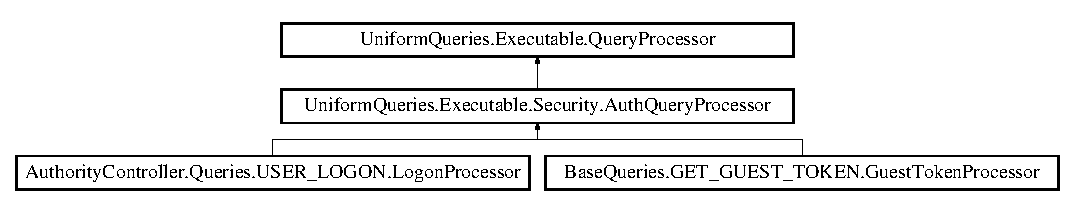
\includegraphics[height=2.326870cm]{dc/d75/class_uniform_queries_1_1_executable_1_1_query_processor}
\end{center}
\end{figure}
\subsection*{Public Member Functions}
\begin{DoxyCompactItemize}
\item 
virtual void \mbox{\hyperlink{class_uniform_queries_1_1_executable_1_1_query_processor_a7cbb30cf1452ec10f246d82145f0d90f}{Terminate\+Authorization\+Task}} ()
\begin{DoxyCompactList}\small\item\em Terminating current started process. \end{DoxyCompactList}\end{DoxyCompactItemize}
\subsection*{Protected Member Functions}
\begin{DoxyCompactItemize}
\item 
void \mbox{\hyperlink{class_uniform_queries_1_1_executable_1_1_query_processor_abe2a2292006829ba3b715b1cfe19f9cb}{Finalize}} (bool result, object args)
\begin{DoxyCompactList}\small\item\em Generate Processing\+Finished event with provided params. \end{DoxyCompactList}\item 
abstract void \mbox{\hyperlink{class_uniform_queries_1_1_executable_1_1_query_processor_a4597c1035fc6bb96f9285cb666655a53}{Server\+Answer\+Handler}} (object controller, object answer)
\begin{DoxyCompactList}\small\item\em Handler that would recive server answer. \end{DoxyCompactList}\end{DoxyCompactItemize}
\subsection*{Properties}
\begin{DoxyCompactItemize}
\item 
bool \mbox{\hyperlink{class_uniform_queries_1_1_executable_1_1_query_processor_a6782b3a610851ec2eabb04b43172b7e0}{Is\+Terminated}}\hspace{0.3cm}{\ttfamily  \mbox{[}get, protected set\mbox{]}}
\begin{DoxyCompactList}\small\item\em Does last auth\textquotesingle{}s task was terminated. \end{DoxyCompactList}\item 
bool \mbox{\hyperlink{class_uniform_queries_1_1_executable_1_1_query_processor_aef7bc3b54884fa1c4f95af2fd542b6c0}{Is\+In\+Progress}}\hspace{0.3cm}{\ttfamily  \mbox{[}get, protected set\mbox{]}}
\begin{DoxyCompactList}\small\item\em Is authrentification in proggress. \end{DoxyCompactList}\end{DoxyCompactItemize}
\subsection*{Events}
\begin{DoxyCompactItemize}
\item 
Action$<$ \mbox{\hyperlink{class_uniform_queries_1_1_executable_1_1_query_processor}{Query\+Processor}}, bool, object $>$ \mbox{\hyperlink{class_uniform_queries_1_1_executable_1_1_query_processor_a87f6d66a2f0bdd9ff0c0a3e66e716efe}{Processing\+Finished}}
\begin{DoxyCompactList}\small\item\em Event that would be called when reciving operation would be finished. \end{DoxyCompactList}\end{DoxyCompactItemize}


\subsection{Detailed Description}
Object that provide base methods that allow to standartize and controll query processing. 



\subsection{Member Function Documentation}
\mbox{\Hypertarget{class_uniform_queries_1_1_executable_1_1_query_processor_abe2a2292006829ba3b715b1cfe19f9cb}\label{class_uniform_queries_1_1_executable_1_1_query_processor_abe2a2292006829ba3b715b1cfe19f9cb}} 
\index{Uniform\+Queries\+::\+Executable\+::\+Query\+Processor@{Uniform\+Queries\+::\+Executable\+::\+Query\+Processor}!Finalize@{Finalize}}
\index{Finalize@{Finalize}!Uniform\+Queries\+::\+Executable\+::\+Query\+Processor@{Uniform\+Queries\+::\+Executable\+::\+Query\+Processor}}
\subsubsection{\texorpdfstring{Finalize()}{Finalize()}}
{\footnotesize\ttfamily void Uniform\+Queries.\+Executable.\+Query\+Processor.\+Finalize (\begin{DoxyParamCaption}\item[{bool}]{result,  }\item[{object}]{args }\end{DoxyParamCaption})\hspace{0.3cm}{\ttfamily [protected]}}



Generate Processing\+Finished event with provided params. 


\begin{DoxyParams}{Parameters}
{\em result} & Resdult of processing.\\
\hline
{\em message} & Shared message.\\
\hline
\end{DoxyParams}
\mbox{\Hypertarget{class_uniform_queries_1_1_executable_1_1_query_processor_a4597c1035fc6bb96f9285cb666655a53}\label{class_uniform_queries_1_1_executable_1_1_query_processor_a4597c1035fc6bb96f9285cb666655a53}} 
\index{Uniform\+Queries\+::\+Executable\+::\+Query\+Processor@{Uniform\+Queries\+::\+Executable\+::\+Query\+Processor}!Server\+Answer\+Handler@{Server\+Answer\+Handler}}
\index{Server\+Answer\+Handler@{Server\+Answer\+Handler}!Uniform\+Queries\+::\+Executable\+::\+Query\+Processor@{Uniform\+Queries\+::\+Executable\+::\+Query\+Processor}}
\subsubsection{\texorpdfstring{Server\+Answer\+Handler()}{ServerAnswerHandler()}}
{\footnotesize\ttfamily abstract void Uniform\+Queries.\+Executable.\+Query\+Processor.\+Server\+Answer\+Handler (\begin{DoxyParamCaption}\item[{object}]{controller,  }\item[{object}]{answer }\end{DoxyParamCaption})\hspace{0.3cm}{\ttfamily [protected]}, {\ttfamily [pure virtual]}}



Handler that would recive server answer. 


\begin{DoxyParams}{Parameters}
{\em line} & \\
\hline
{\em answer} & \\
\hline
\end{DoxyParams}


Implemented in \mbox{\hyperlink{class_uniform_queries_1_1_executable_1_1_security_1_1_auth_query_processor_a4693289bf81ca5d98fe8f5678a7c4b87}{Uniform\+Queries.\+Executable.\+Security.\+Auth\+Query\+Processor}}.

\mbox{\Hypertarget{class_uniform_queries_1_1_executable_1_1_query_processor_a7cbb30cf1452ec10f246d82145f0d90f}\label{class_uniform_queries_1_1_executable_1_1_query_processor_a7cbb30cf1452ec10f246d82145f0d90f}} 
\index{Uniform\+Queries\+::\+Executable\+::\+Query\+Processor@{Uniform\+Queries\+::\+Executable\+::\+Query\+Processor}!Terminate\+Authorization\+Task@{Terminate\+Authorization\+Task}}
\index{Terminate\+Authorization\+Task@{Terminate\+Authorization\+Task}!Uniform\+Queries\+::\+Executable\+::\+Query\+Processor@{Uniform\+Queries\+::\+Executable\+::\+Query\+Processor}}
\subsubsection{\texorpdfstring{Terminate\+Authorization\+Task()}{TerminateAuthorizationTask()}}
{\footnotesize\ttfamily virtual void Uniform\+Queries.\+Executable.\+Query\+Processor.\+Terminate\+Authorization\+Task (\begin{DoxyParamCaption}{ }\end{DoxyParamCaption})\hspace{0.3cm}{\ttfamily [virtual]}}



Terminating current started process. 



\subsection{Property Documentation}
\mbox{\Hypertarget{class_uniform_queries_1_1_executable_1_1_query_processor_aef7bc3b54884fa1c4f95af2fd542b6c0}\label{class_uniform_queries_1_1_executable_1_1_query_processor_aef7bc3b54884fa1c4f95af2fd542b6c0}} 
\index{Uniform\+Queries\+::\+Executable\+::\+Query\+Processor@{Uniform\+Queries\+::\+Executable\+::\+Query\+Processor}!Is\+In\+Progress@{Is\+In\+Progress}}
\index{Is\+In\+Progress@{Is\+In\+Progress}!Uniform\+Queries\+::\+Executable\+::\+Query\+Processor@{Uniform\+Queries\+::\+Executable\+::\+Query\+Processor}}
\subsubsection{\texorpdfstring{Is\+In\+Progress}{IsInProgress}}
{\footnotesize\ttfamily bool Uniform\+Queries.\+Executable.\+Query\+Processor.\+Is\+In\+Progress\hspace{0.3cm}{\ttfamily [get]}, {\ttfamily [protected set]}}



Is authrentification in proggress. 

\mbox{\Hypertarget{class_uniform_queries_1_1_executable_1_1_query_processor_a6782b3a610851ec2eabb04b43172b7e0}\label{class_uniform_queries_1_1_executable_1_1_query_processor_a6782b3a610851ec2eabb04b43172b7e0}} 
\index{Uniform\+Queries\+::\+Executable\+::\+Query\+Processor@{Uniform\+Queries\+::\+Executable\+::\+Query\+Processor}!Is\+Terminated@{Is\+Terminated}}
\index{Is\+Terminated@{Is\+Terminated}!Uniform\+Queries\+::\+Executable\+::\+Query\+Processor@{Uniform\+Queries\+::\+Executable\+::\+Query\+Processor}}
\subsubsection{\texorpdfstring{Is\+Terminated}{IsTerminated}}
{\footnotesize\ttfamily bool Uniform\+Queries.\+Executable.\+Query\+Processor.\+Is\+Terminated\hspace{0.3cm}{\ttfamily [get]}, {\ttfamily [protected set]}}



Does last auth\textquotesingle{}s task was terminated. 



\subsection{Event Documentation}
\mbox{\Hypertarget{class_uniform_queries_1_1_executable_1_1_query_processor_a87f6d66a2f0bdd9ff0c0a3e66e716efe}\label{class_uniform_queries_1_1_executable_1_1_query_processor_a87f6d66a2f0bdd9ff0c0a3e66e716efe}} 
\index{Uniform\+Queries\+::\+Executable\+::\+Query\+Processor@{Uniform\+Queries\+::\+Executable\+::\+Query\+Processor}!Processing\+Finished@{Processing\+Finished}}
\index{Processing\+Finished@{Processing\+Finished}!Uniform\+Queries\+::\+Executable\+::\+Query\+Processor@{Uniform\+Queries\+::\+Executable\+::\+Query\+Processor}}
\subsubsection{\texorpdfstring{Processing\+Finished}{ProcessingFinished}}
{\footnotesize\ttfamily Action$<$\mbox{\hyperlink{class_uniform_queries_1_1_executable_1_1_query_processor}{Query\+Processor}}, bool, object$>$ Uniform\+Queries.\+Executable.\+Query\+Processor.\+Processing\+Finished}



Event that would be called when reciving operation would be finished. 

\mbox{\hyperlink{class_uniform_queries_1_1_executable_1_1_query_processor}{Executable.\+Query\+Processor}} -\/ reference to this processor. bool -\/ result od operation object -\/ object shared by processor. 

The documentation for this class was generated from the following file\+:\begin{DoxyCompactItemize}
\item 
D\+:/\+Work/\+Git\+Hub/doloro-\/networking-\/framework/\+Core/\+Uniform\+Queries/\+Executable/Query\+Processor.\+cs\end{DoxyCompactItemize}

\hypertarget{class_pipes_provider_1_1_networking_1_1_routing_1_1_relay_instruction}{}\section{Pipes\+Provider.\+Networking.\+Routing.\+Relay\+Instruction Class Reference}
\label{class_pipes_provider_1_1_networking_1_1_routing_1_1_relay_instruction}\index{Pipes\+Provider.\+Networking.\+Routing.\+Relay\+Instruction@{Pipes\+Provider.\+Networking.\+Routing.\+Relay\+Instruction}}


\mbox{\hyperlink{class_pipes_provider_1_1_networking_1_1_routing_1_1_instruction}{Instruction}} that allow retranslate broadcasting via servers chain.  


Inheritance diagram for Pipes\+Provider.\+Networking.\+Routing.\+Relay\+Instruction\+:\begin{figure}[H]
\begin{center}
\leavevmode
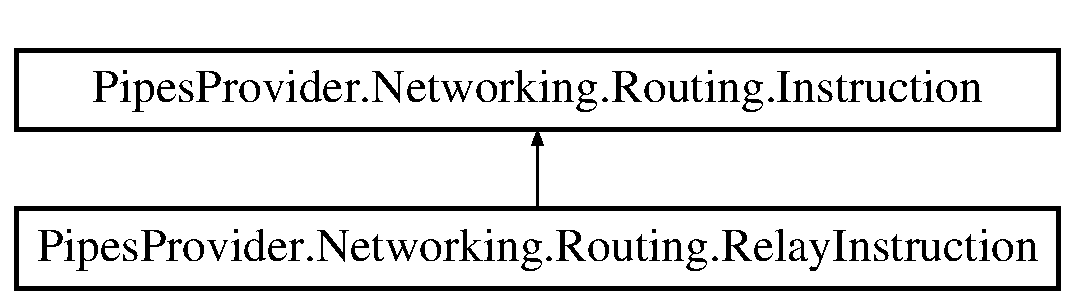
\includegraphics[height=2.000000cm]{de/d56/class_pipes_provider_1_1_networking_1_1_routing_1_1_relay_instruction}
\end{center}
\end{figure}
\subsection*{Static Public Member Functions}
\begin{DoxyCompactItemize}
\item 
static bool \mbox{\hyperlink{class_pipes_provider_1_1_networking_1_1_routing_1_1_relay_instruction_a31f5ae59274888144f030d36e6b0a048}{Try\+To\+Detect\+Target}} (I\+Enumerable$<$ \mbox{\hyperlink{class_pipes_provider_1_1_networking_1_1_routing_1_1_instruction}{Instruction}} $>$ collection, string \mbox{\hyperlink{class_pipes_provider_1_1_networking_1_1_routing_1_1_relay_instruction_ab5f83b58775b783a3dc4d4ad2d9ffb81}{entry\+Pipe\+Name}}, out \mbox{\hyperlink{class_pipes_provider_1_1_networking_1_1_routing_1_1_relay_instruction}{Relay\+Instruction}} relay\+Instruction)
\begin{DoxyCompactList}\small\item\em Trying to find suitable instruction for transmisting pipe. \end{DoxyCompactList}\item 
static \mbox{\hyperlink{class_pipes_provider_1_1_networking_1_1_routing_1_1_relay_instruction}{Relay\+Instruction}} \mbox{\hyperlink{class_pipes_provider_1_1_networking_1_1_routing_1_1_relay_instruction_a94279d5a766e562f152ce612827fcbe8}{Detect\+Target}} (I\+Enumerable$<$ \mbox{\hyperlink{class_pipes_provider_1_1_networking_1_1_routing_1_1_instruction}{Instruction}} $>$ collection, string \mbox{\hyperlink{class_pipes_provider_1_1_networking_1_1_routing_1_1_relay_instruction_ab5f83b58775b783a3dc4d4ad2d9ffb81}{entry\+Pipe\+Name}})
\begin{DoxyCompactList}\small\item\em Looking for suitable instruction for transmisting pipe. In case if not found returning null. \end{DoxyCompactList}\end{DoxyCompactItemize}
\subsection*{Public Attributes}
\begin{DoxyCompactItemize}
\item 
string \mbox{\hyperlink{class_pipes_provider_1_1_networking_1_1_routing_1_1_relay_instruction_ab5f83b58775b783a3dc4d4ad2d9ffb81}{entry\+Pipe\+Name}} = \char`\"{}broadcasting\char`\"{}
\begin{DoxyCompactList}\small\item\em Name of pipe started on server that would relay broadcasting from target server. Target server must be broadcasting one. \end{DoxyCompactList}\end{DoxyCompactItemize}
\subsection*{Additional Inherited Members}


\subsection{Detailed Description}
\mbox{\hyperlink{class_pipes_provider_1_1_networking_1_1_routing_1_1_instruction}{Instruction}} that allow retranslate broadcasting via servers chain. 



\subsection{Member Function Documentation}
\mbox{\Hypertarget{class_pipes_provider_1_1_networking_1_1_routing_1_1_relay_instruction_a94279d5a766e562f152ce612827fcbe8}\label{class_pipes_provider_1_1_networking_1_1_routing_1_1_relay_instruction_a94279d5a766e562f152ce612827fcbe8}} 
\index{Pipes\+Provider\+::\+Networking\+::\+Routing\+::\+Relay\+Instruction@{Pipes\+Provider\+::\+Networking\+::\+Routing\+::\+Relay\+Instruction}!Detect\+Target@{Detect\+Target}}
\index{Detect\+Target@{Detect\+Target}!Pipes\+Provider\+::\+Networking\+::\+Routing\+::\+Relay\+Instruction@{Pipes\+Provider\+::\+Networking\+::\+Routing\+::\+Relay\+Instruction}}
\subsubsection{\texorpdfstring{Detect\+Target()}{DetectTarget()}}
{\footnotesize\ttfamily static \mbox{\hyperlink{class_pipes_provider_1_1_networking_1_1_routing_1_1_relay_instruction}{Relay\+Instruction}} Pipes\+Provider.\+Networking.\+Routing.\+Relay\+Instruction.\+Detect\+Target (\begin{DoxyParamCaption}\item[{I\+Enumerable$<$ \mbox{\hyperlink{class_pipes_provider_1_1_networking_1_1_routing_1_1_instruction}{Instruction}} $>$}]{collection,  }\item[{string}]{entry\+Pipe\+Name }\end{DoxyParamCaption})\hspace{0.3cm}{\ttfamily [static]}}



Looking for suitable instruction for transmisting pipe. In case if not found returning null. 


\begin{DoxyParams}{Parameters}
{\em collection} & Collection of routing instructions that could contains target \mbox{\hyperlink{class_pipes_provider_1_1_networking_1_1_routing_1_1_relay_instruction}{Relay\+Instruction}}.\\
\hline
{\em entry\+Pipe\+Name} & Name of relay pipe that recive broadcasting relay request.\\
\hline
\end{DoxyParams}
\begin{DoxyReturn}{Returns}
$>$A found instruction. Null if not found.
\end{DoxyReturn}
\mbox{\Hypertarget{class_pipes_provider_1_1_networking_1_1_routing_1_1_relay_instruction_a31f5ae59274888144f030d36e6b0a048}\label{class_pipes_provider_1_1_networking_1_1_routing_1_1_relay_instruction_a31f5ae59274888144f030d36e6b0a048}} 
\index{Pipes\+Provider\+::\+Networking\+::\+Routing\+::\+Relay\+Instruction@{Pipes\+Provider\+::\+Networking\+::\+Routing\+::\+Relay\+Instruction}!Try\+To\+Detect\+Target@{Try\+To\+Detect\+Target}}
\index{Try\+To\+Detect\+Target@{Try\+To\+Detect\+Target}!Pipes\+Provider\+::\+Networking\+::\+Routing\+::\+Relay\+Instruction@{Pipes\+Provider\+::\+Networking\+::\+Routing\+::\+Relay\+Instruction}}
\subsubsection{\texorpdfstring{Try\+To\+Detect\+Target()}{TryToDetectTarget()}}
{\footnotesize\ttfamily static bool Pipes\+Provider.\+Networking.\+Routing.\+Relay\+Instruction.\+Try\+To\+Detect\+Target (\begin{DoxyParamCaption}\item[{I\+Enumerable$<$ \mbox{\hyperlink{class_pipes_provider_1_1_networking_1_1_routing_1_1_instruction}{Instruction}} $>$}]{collection,  }\item[{string}]{entry\+Pipe\+Name,  }\item[{out \mbox{\hyperlink{class_pipes_provider_1_1_networking_1_1_routing_1_1_relay_instruction}{Relay\+Instruction}}}]{relay\+Instruction }\end{DoxyParamCaption})\hspace{0.3cm}{\ttfamily [static]}}



Trying to find suitable instruction for transmisting pipe. 


\begin{DoxyParams}{Parameters}
{\em collection} & Collection of routing instructions that could contains target \mbox{\hyperlink{class_pipes_provider_1_1_networking_1_1_routing_1_1_relay_instruction}{Relay\+Instruction}}.\\
\hline
{\em entry\+Pipe\+Name} & Name of relay pipe that recive broadcasting relay request.\\
\hline
{\em relay\+Instruction} & A found instruction. Null if not found.\\
\hline
\end{DoxyParams}
\begin{DoxyReturn}{Returns}
Resut of search.
\end{DoxyReturn}


\subsection{Member Data Documentation}
\mbox{\Hypertarget{class_pipes_provider_1_1_networking_1_1_routing_1_1_relay_instruction_ab5f83b58775b783a3dc4d4ad2d9ffb81}\label{class_pipes_provider_1_1_networking_1_1_routing_1_1_relay_instruction_ab5f83b58775b783a3dc4d4ad2d9ffb81}} 
\index{Pipes\+Provider\+::\+Networking\+::\+Routing\+::\+Relay\+Instruction@{Pipes\+Provider\+::\+Networking\+::\+Routing\+::\+Relay\+Instruction}!entry\+Pipe\+Name@{entry\+Pipe\+Name}}
\index{entry\+Pipe\+Name@{entry\+Pipe\+Name}!Pipes\+Provider\+::\+Networking\+::\+Routing\+::\+Relay\+Instruction@{Pipes\+Provider\+::\+Networking\+::\+Routing\+::\+Relay\+Instruction}}
\subsubsection{\texorpdfstring{entry\+Pipe\+Name}{entryPipeName}}
{\footnotesize\ttfamily string Pipes\+Provider.\+Networking.\+Routing.\+Relay\+Instruction.\+entry\+Pipe\+Name = \char`\"{}broadcasting\char`\"{}}



Name of pipe started on server that would relay broadcasting from target server. Target server must be broadcasting one. 

Shame\+: client -\/$>$ relay-\/server-\/ip.\+entry\+Pipe\+Name -\/$>$ routing\+Ip.\+pipe\+Name 

The documentation for this class was generated from the following file\+:\begin{DoxyCompactItemize}
\item 
D\+:/\+Work/\+Git\+Hub/doloro-\/networking-\/framework/\+Core/\+D\+N\+F\+Core/\+Uniform\+Client/\+Extensions/\+Pipes\+Provider/Relay\+Instruction.\+cs\end{DoxyCompactItemize}

\hypertarget{class_uniform_server_1_1_standard_1_1_relay_server}{}\section{Uniform\+Server.\+Standard.\+Relay\+Server Class Reference}
\label{class_uniform_server_1_1_standard_1_1_relay_server}\index{Uniform\+Server.\+Standard.\+Relay\+Server@{Uniform\+Server.\+Standard.\+Relay\+Server}}


Server that provide A\+PI for relaying of transmission.  


Inheritance diagram for Uniform\+Server.\+Standard.\+Relay\+Server\+:\begin{figure}[H]
\begin{center}
\leavevmode
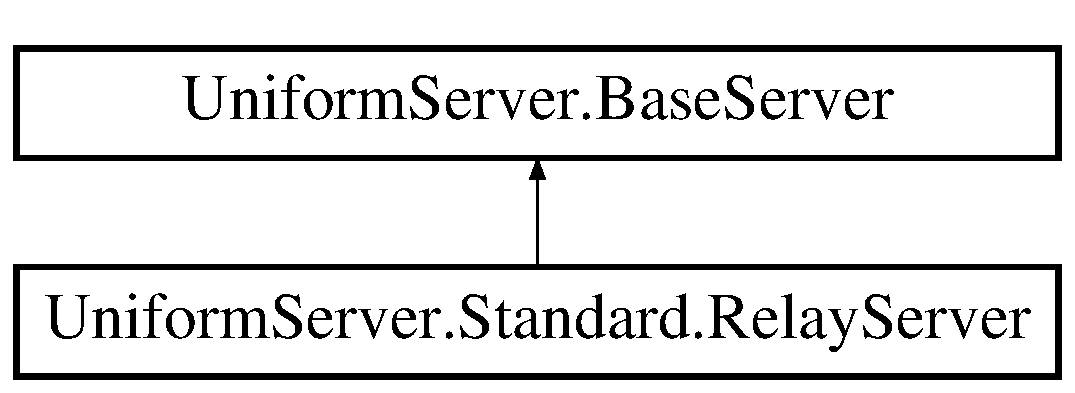
\includegraphics[height=2.000000cm]{d0/d04/class_uniform_server_1_1_standard_1_1_relay_server}
\end{center}
\end{figure}
\subsection*{Static Public Member Functions}
\begin{DoxyCompactItemize}
\item 
static \mbox{\hyperlink{class_uniform_server_1_1_standard_1_1_relay_server}{Relay\+Server}} \mbox{\hyperlink{class_uniform_server_1_1_standard_1_1_relay_server_a95fbce307be04e63d120a674f7bde0f3}{Establish\+Broadcasting\+Relay\+Server}} (\mbox{\hyperlink{class_pipes_provider_1_1_networking_1_1_routing_1_1_relay_instruction}{Relay\+Instruction}} isntruction)
\begin{DoxyCompactList}\small\item\em Establish server suitable provided instruction that would retranslate broadcasting from target server. \end{DoxyCompactList}\item 
static string \mbox{\hyperlink{class_uniform_server_1_1_standard_1_1_relay_server_a5306cb2ee3b40c50785283c4d4e5d387}{Query\+Handler\+\_\+\+Broadcasting\+Relay}} (\mbox{\hyperlink{class_pipes_provider_1_1_server_1_1_transmission_controllers_1_1_broadcasting_server_transmission_controller}{Broadcasting\+Server\+Transmission\+Controller}} controller)
\begin{DoxyCompactList}\small\item\em Redirect recived query from current server to other. \end{DoxyCompactList}\item 
static \mbox{\hyperlink{class_uniform_server_1_1_standard_1_1_relay_server}{Relay\+Server}} \mbox{\hyperlink{class_uniform_server_1_1_standard_1_1_relay_server_a6a3e3701a479f5ee4846d79c4a153f7e}{Establish\+Duplex\+Relay\+Server}} (\mbox{\hyperlink{class_pipes_provider_1_1_networking_1_1_routing_1_1_relay_instruction}{Relay\+Instruction}} isntruction)
\begin{DoxyCompactList}\small\item\em Establishing server that would recive client\textquotesingle{}s server and forwarding it to target servers by using routing table. \end{DoxyCompactList}\item 
static void \mbox{\hyperlink{class_uniform_server_1_1_standard_1_1_relay_server_a96a666ec31626f2e1a3f2f1d4d444366}{Query\+Handler\+\_\+\+Duplex\+Relay}} (\mbox{\hyperlink{class_pipes_provider_1_1_server_1_1_transmission_controllers_1_1_base_server_transmission_controller}{Base\+Server\+Transmission\+Controller}} \+\_\+, string query)
\begin{DoxyCompactList}\small\item\em Redirect recived query from current server to other. \end{DoxyCompactList}\end{DoxyCompactItemize}
\subsection*{Static Protected Member Functions}
\begin{DoxyCompactItemize}
\item 
static void \mbox{\hyperlink{class_uniform_server_1_1_standard_1_1_relay_server_a5940f8db2d25ff38ecdb7e5ab74063f9}{Threading\+Server\+Loop\+\_\+\+Broadcasting\+Relay}} (object server)
\begin{DoxyCompactList}\small\item\em Starting the server loop that will control relay query handler. \end{DoxyCompactList}\item 
static void \mbox{\hyperlink{class_uniform_server_1_1_standard_1_1_relay_server_a8612def1490dc0c8e0b4535a54a09c18}{Threading\+Server\+Loop\+\_\+\+Duplex\+Relay}} (object server)
\begin{DoxyCompactList}\small\item\em Starting the server loop that will control relay query handler. \end{DoxyCompactList}\end{DoxyCompactItemize}
\subsection*{Additional Inherited Members}


\subsection{Detailed Description}
Server that provide A\+PI for relaying of transmission. 



\subsection{Member Function Documentation}
\mbox{\Hypertarget{class_uniform_server_1_1_standard_1_1_relay_server_a95fbce307be04e63d120a674f7bde0f3}\label{class_uniform_server_1_1_standard_1_1_relay_server_a95fbce307be04e63d120a674f7bde0f3}} 
\index{Uniform\+Server\+::\+Standard\+::\+Relay\+Server@{Uniform\+Server\+::\+Standard\+::\+Relay\+Server}!Establish\+Broadcasting\+Relay\+Server@{Establish\+Broadcasting\+Relay\+Server}}
\index{Establish\+Broadcasting\+Relay\+Server@{Establish\+Broadcasting\+Relay\+Server}!Uniform\+Server\+::\+Standard\+::\+Relay\+Server@{Uniform\+Server\+::\+Standard\+::\+Relay\+Server}}
\subsubsection{\texorpdfstring{Establish\+Broadcasting\+Relay\+Server()}{EstablishBroadcastingRelayServer()}}
{\footnotesize\ttfamily static \mbox{\hyperlink{class_uniform_server_1_1_standard_1_1_relay_server}{Relay\+Server}} Uniform\+Server.\+Standard.\+Relay\+Server.\+Establish\+Broadcasting\+Relay\+Server (\begin{DoxyParamCaption}\item[{\mbox{\hyperlink{class_pipes_provider_1_1_networking_1_1_routing_1_1_relay_instruction}{Relay\+Instruction}}}]{isntruction }\end{DoxyParamCaption})\hspace{0.3cm}{\ttfamily [static]}}



Establish server suitable provided instruction that would retranslate broadcasting from target server. 


\begin{DoxyParams}{Parameters}
{\em relay\+Instruction} & Instruction that contain relay params.\\
\hline
\end{DoxyParams}
\begin{DoxyReturn}{Returns}
Established server.
\end{DoxyReturn}
\mbox{\Hypertarget{class_uniform_server_1_1_standard_1_1_relay_server_a6a3e3701a479f5ee4846d79c4a153f7e}\label{class_uniform_server_1_1_standard_1_1_relay_server_a6a3e3701a479f5ee4846d79c4a153f7e}} 
\index{Uniform\+Server\+::\+Standard\+::\+Relay\+Server@{Uniform\+Server\+::\+Standard\+::\+Relay\+Server}!Establish\+Duplex\+Relay\+Server@{Establish\+Duplex\+Relay\+Server}}
\index{Establish\+Duplex\+Relay\+Server@{Establish\+Duplex\+Relay\+Server}!Uniform\+Server\+::\+Standard\+::\+Relay\+Server@{Uniform\+Server\+::\+Standard\+::\+Relay\+Server}}
\subsubsection{\texorpdfstring{Establish\+Duplex\+Relay\+Server()}{EstablishDuplexRelayServer()}}
{\footnotesize\ttfamily static \mbox{\hyperlink{class_uniform_server_1_1_standard_1_1_relay_server}{Relay\+Server}} Uniform\+Server.\+Standard.\+Relay\+Server.\+Establish\+Duplex\+Relay\+Server (\begin{DoxyParamCaption}\item[{\mbox{\hyperlink{class_pipes_provider_1_1_networking_1_1_routing_1_1_relay_instruction}{Relay\+Instruction}}}]{isntruction }\end{DoxyParamCaption})\hspace{0.3cm}{\ttfamily [static]}}



Establishing server that would recive client\textquotesingle{}s server and forwarding it to target servers by using routing table. 


\begin{DoxyParams}{Parameters}
{\em isntruction} & Instruction that contain relay params.\\
\hline
\end{DoxyParams}
\begin{DoxyReturn}{Returns}
Established server.
\end{DoxyReturn}
\mbox{\Hypertarget{class_uniform_server_1_1_standard_1_1_relay_server_a5306cb2ee3b40c50785283c4d4e5d387}\label{class_uniform_server_1_1_standard_1_1_relay_server_a5306cb2ee3b40c50785283c4d4e5d387}} 
\index{Uniform\+Server\+::\+Standard\+::\+Relay\+Server@{Uniform\+Server\+::\+Standard\+::\+Relay\+Server}!Query\+Handler\+\_\+\+Broadcasting\+Relay@{Query\+Handler\+\_\+\+Broadcasting\+Relay}}
\index{Query\+Handler\+\_\+\+Broadcasting\+Relay@{Query\+Handler\+\_\+\+Broadcasting\+Relay}!Uniform\+Server\+::\+Standard\+::\+Relay\+Server@{Uniform\+Server\+::\+Standard\+::\+Relay\+Server}}
\subsubsection{\texorpdfstring{Query\+Handler\+\_\+\+Broadcasting\+Relay()}{QueryHandler\_BroadcastingRelay()}}
{\footnotesize\ttfamily static string Uniform\+Server.\+Standard.\+Relay\+Server.\+Query\+Handler\+\_\+\+Broadcasting\+Relay (\begin{DoxyParamCaption}\item[{\mbox{\hyperlink{class_pipes_provider_1_1_server_1_1_transmission_controllers_1_1_broadcasting_server_transmission_controller}{Broadcasting\+Server\+Transmission\+Controller}}}]{controller }\end{DoxyParamCaption})\hspace{0.3cm}{\ttfamily [static]}}



Redirect recived query from current server to other. 


\begin{DoxyParams}{Parameters}
{\em \+\_\+} & \\
\hline
{\em query} & \\
\hline
\end{DoxyParams}
\mbox{\Hypertarget{class_uniform_server_1_1_standard_1_1_relay_server_a96a666ec31626f2e1a3f2f1d4d444366}\label{class_uniform_server_1_1_standard_1_1_relay_server_a96a666ec31626f2e1a3f2f1d4d444366}} 
\index{Uniform\+Server\+::\+Standard\+::\+Relay\+Server@{Uniform\+Server\+::\+Standard\+::\+Relay\+Server}!Query\+Handler\+\_\+\+Duplex\+Relay@{Query\+Handler\+\_\+\+Duplex\+Relay}}
\index{Query\+Handler\+\_\+\+Duplex\+Relay@{Query\+Handler\+\_\+\+Duplex\+Relay}!Uniform\+Server\+::\+Standard\+::\+Relay\+Server@{Uniform\+Server\+::\+Standard\+::\+Relay\+Server}}
\subsubsection{\texorpdfstring{Query\+Handler\+\_\+\+Duplex\+Relay()}{QueryHandler\_DuplexRelay()}}
{\footnotesize\ttfamily static void Uniform\+Server.\+Standard.\+Relay\+Server.\+Query\+Handler\+\_\+\+Duplex\+Relay (\begin{DoxyParamCaption}\item[{\mbox{\hyperlink{class_pipes_provider_1_1_server_1_1_transmission_controllers_1_1_base_server_transmission_controller}{Base\+Server\+Transmission\+Controller}}}]{\+\_\+,  }\item[{string}]{query }\end{DoxyParamCaption})\hspace{0.3cm}{\ttfamily [static]}}



Redirect recived query from current server to other. 


\begin{DoxyParams}{Parameters}
{\em \+\_\+} & \\
\hline
{\em query} & \\
\hline
\end{DoxyParams}
\mbox{\Hypertarget{class_uniform_server_1_1_standard_1_1_relay_server_a5940f8db2d25ff38ecdb7e5ab74063f9}\label{class_uniform_server_1_1_standard_1_1_relay_server_a5940f8db2d25ff38ecdb7e5ab74063f9}} 
\index{Uniform\+Server\+::\+Standard\+::\+Relay\+Server@{Uniform\+Server\+::\+Standard\+::\+Relay\+Server}!Threading\+Server\+Loop\+\_\+\+Broadcasting\+Relay@{Threading\+Server\+Loop\+\_\+\+Broadcasting\+Relay}}
\index{Threading\+Server\+Loop\+\_\+\+Broadcasting\+Relay@{Threading\+Server\+Loop\+\_\+\+Broadcasting\+Relay}!Uniform\+Server\+::\+Standard\+::\+Relay\+Server@{Uniform\+Server\+::\+Standard\+::\+Relay\+Server}}
\subsubsection{\texorpdfstring{Threading\+Server\+Loop\+\_\+\+Broadcasting\+Relay()}{ThreadingServerLoop\_BroadcastingRelay()}}
{\footnotesize\ttfamily static void Uniform\+Server.\+Standard.\+Relay\+Server.\+Threading\+Server\+Loop\+\_\+\+Broadcasting\+Relay (\begin{DoxyParamCaption}\item[{object}]{server }\end{DoxyParamCaption})\hspace{0.3cm}{\ttfamily [static]}, {\ttfamily [protected]}}



Starting the server loop that will control relay query handler. 

\mbox{\Hypertarget{class_uniform_server_1_1_standard_1_1_relay_server_a8612def1490dc0c8e0b4535a54a09c18}\label{class_uniform_server_1_1_standard_1_1_relay_server_a8612def1490dc0c8e0b4535a54a09c18}} 
\index{Uniform\+Server\+::\+Standard\+::\+Relay\+Server@{Uniform\+Server\+::\+Standard\+::\+Relay\+Server}!Threading\+Server\+Loop\+\_\+\+Duplex\+Relay@{Threading\+Server\+Loop\+\_\+\+Duplex\+Relay}}
\index{Threading\+Server\+Loop\+\_\+\+Duplex\+Relay@{Threading\+Server\+Loop\+\_\+\+Duplex\+Relay}!Uniform\+Server\+::\+Standard\+::\+Relay\+Server@{Uniform\+Server\+::\+Standard\+::\+Relay\+Server}}
\subsubsection{\texorpdfstring{Threading\+Server\+Loop\+\_\+\+Duplex\+Relay()}{ThreadingServerLoop\_DuplexRelay()}}
{\footnotesize\ttfamily static void Uniform\+Server.\+Standard.\+Relay\+Server.\+Threading\+Server\+Loop\+\_\+\+Duplex\+Relay (\begin{DoxyParamCaption}\item[{object}]{server }\end{DoxyParamCaption})\hspace{0.3cm}{\ttfamily [static]}, {\ttfamily [protected]}}



Starting the server loop that will control relay query handler. 



The documentation for this class was generated from the following file\+:\begin{DoxyCompactItemize}
\item 
D\+:/\+Work/\+Git\+Hub/doloro-\/networking-\/framework/\+Core/\+D\+N\+F\+Core/\+Uniform\+Server/\+Providers/\+Standard/Relay\+Server.\+cs\end{DoxyCompactItemize}

\hypertarget{class_pipes_provider_1_1_networking_1_1_routing_1_1_routing_table}{}\section{Pipes\+Provider.\+Networking.\+Routing.\+Routing\+Table Class Reference}
\label{class_pipes_provider_1_1_networking_1_1_routing_1_1_routing_table}\index{Pipes\+Provider.\+Networking.\+Routing.\+Routing\+Table@{Pipes\+Provider.\+Networking.\+Routing.\+Routing\+Table}}


Object that contain routing instgructions. Provide A\+PI to work with file system.  


\subsection*{Public Member Functions}
\begin{DoxyCompactItemize}
\item 
bool \mbox{\hyperlink{class_pipes_provider_1_1_networking_1_1_routing_1_1_routing_table_afa326622fc49d66bcd375c08b2f6ff8b}{Try\+Get\+Routing\+Instruction}} (string query, out \mbox{\hyperlink{class_pipes_provider_1_1_networking_1_1_routing_1_1_instruction}{Instruction}} instruction)
\begin{DoxyCompactList}\small\item\em Trying to find target routing instruction. \end{DoxyCompactList}\end{DoxyCompactItemize}
\subsection*{Static Public Member Functions}
\begin{DoxyCompactItemize}
\item 
static \mbox{\hyperlink{class_pipes_provider_1_1_networking_1_1_routing_1_1_routing_table}{Routing\+Table}} \mbox{\hyperlink{class_pipes_provider_1_1_networking_1_1_routing_1_1_routing_table_a13c2778abb1d14e7e8e4a2ae51d315ac}{Load\+Routing\+Tables}} (string directory, Search\+Option search\+Option)
\begin{DoxyCompactList}\small\item\em Trying to load all routing tables from durectory. You could have several X\+ML serialized routing tables. This way allow to share it via plugins. \end{DoxyCompactList}\item 
static void \mbox{\hyperlink{class_pipes_provider_1_1_networking_1_1_routing_1_1_routing_table_a1fe9c42819cd5c5210b254c0d868b336}{Save\+Routing\+Table}} (\mbox{\hyperlink{class_pipes_provider_1_1_networking_1_1_routing_1_1_routing_table}{Routing\+Table}} table, string directory, string name)
\begin{DoxyCompactList}\small\item\em Save routing table by directory. \end{DoxyCompactList}\item 
static \mbox{\hyperlink{class_pipes_provider_1_1_networking_1_1_routing_1_1_routing_table}{Routing\+Table}} \mbox{\hyperlink{class_pipes_provider_1_1_networking_1_1_routing_1_1_routing_table_a515b9ad19dc868afb6d47c762064fd96}{operator+}} (\mbox{\hyperlink{class_pipes_provider_1_1_networking_1_1_routing_1_1_routing_table}{Routing\+Table}} table0, \mbox{\hyperlink{class_pipes_provider_1_1_networking_1_1_routing_1_1_routing_table}{Routing\+Table}} table1)
\begin{DoxyCompactList}\small\item\em Adding instruction from second table to first one. \end{DoxyCompactList}\end{DoxyCompactItemize}
\subsection*{Public Attributes}
\begin{DoxyCompactItemize}
\item 
List$<$ \mbox{\hyperlink{class_pipes_provider_1_1_networking_1_1_routing_1_1_instruction}{Instruction}} $>$ \mbox{\hyperlink{class_pipes_provider_1_1_networking_1_1_routing_1_1_routing_table_a1a2c8459b4805d7ee1e81698a389f3f7}{intructions}} = new List$<$\mbox{\hyperlink{class_pipes_provider_1_1_networking_1_1_routing_1_1_instruction}{Instruction}}$>$()
\begin{DoxyCompactList}\small\item\em List that contain routing instructions. \end{DoxyCompactList}\end{DoxyCompactItemize}
\subsection*{Properties}
\begin{DoxyCompactItemize}
\item 
string \mbox{\hyperlink{class_pipes_provider_1_1_networking_1_1_routing_1_1_routing_table_af756c825762d5434f5b934a1c1b2d3eb}{Source\+Path}}\hspace{0.3cm}{\ttfamily  \mbox{[}get, set\mbox{]}}
\begin{DoxyCompactList}\small\item\em Path from was loaded tis table. \end{DoxyCompactList}\end{DoxyCompactItemize}


\subsection{Detailed Description}
Object that contain routing instgructions. Provide A\+PI to work with file system. 



\subsection{Member Function Documentation}
\mbox{\Hypertarget{class_pipes_provider_1_1_networking_1_1_routing_1_1_routing_table_a13c2778abb1d14e7e8e4a2ae51d315ac}\label{class_pipes_provider_1_1_networking_1_1_routing_1_1_routing_table_a13c2778abb1d14e7e8e4a2ae51d315ac}} 
\index{Pipes\+Provider\+::\+Networking\+::\+Routing\+::\+Routing\+Table@{Pipes\+Provider\+::\+Networking\+::\+Routing\+::\+Routing\+Table}!Load\+Routing\+Tables@{Load\+Routing\+Tables}}
\index{Load\+Routing\+Tables@{Load\+Routing\+Tables}!Pipes\+Provider\+::\+Networking\+::\+Routing\+::\+Routing\+Table@{Pipes\+Provider\+::\+Networking\+::\+Routing\+::\+Routing\+Table}}
\subsubsection{\texorpdfstring{Load\+Routing\+Tables()}{LoadRoutingTables()}}
{\footnotesize\ttfamily static \mbox{\hyperlink{class_pipes_provider_1_1_networking_1_1_routing_1_1_routing_table}{Routing\+Table}} Pipes\+Provider.\+Networking.\+Routing.\+Routing\+Table.\+Load\+Routing\+Tables (\begin{DoxyParamCaption}\item[{string}]{directory,  }\item[{Search\+Option}]{search\+Option }\end{DoxyParamCaption})\hspace{0.3cm}{\ttfamily [static]}}



Trying to load all routing tables from durectory. You could have several X\+ML serialized routing tables. This way allow to share it via plugins. 


\begin{DoxyParams}{Parameters}
{\em directory} & Root folder.\\
\hline
{\em search\+Option} & Defind does search will applied to child foldeers.\\
\hline
\end{DoxyParams}
\begin{DoxyReturn}{Returns}

\end{DoxyReturn}
\mbox{\Hypertarget{class_pipes_provider_1_1_networking_1_1_routing_1_1_routing_table_a515b9ad19dc868afb6d47c762064fd96}\label{class_pipes_provider_1_1_networking_1_1_routing_1_1_routing_table_a515b9ad19dc868afb6d47c762064fd96}} 
\index{Pipes\+Provider\+::\+Networking\+::\+Routing\+::\+Routing\+Table@{Pipes\+Provider\+::\+Networking\+::\+Routing\+::\+Routing\+Table}!operator+@{operator+}}
\index{operator+@{operator+}!Pipes\+Provider\+::\+Networking\+::\+Routing\+::\+Routing\+Table@{Pipes\+Provider\+::\+Networking\+::\+Routing\+::\+Routing\+Table}}
\subsubsection{\texorpdfstring{operator+()}{operator+()}}
{\footnotesize\ttfamily static \mbox{\hyperlink{class_pipes_provider_1_1_networking_1_1_routing_1_1_routing_table}{Routing\+Table}} Pipes\+Provider.\+Networking.\+Routing.\+Routing\+Table.\+operator+ (\begin{DoxyParamCaption}\item[{\mbox{\hyperlink{class_pipes_provider_1_1_networking_1_1_routing_1_1_routing_table}{Routing\+Table}}}]{table0,  }\item[{\mbox{\hyperlink{class_pipes_provider_1_1_networking_1_1_routing_1_1_routing_table}{Routing\+Table}}}]{table1 }\end{DoxyParamCaption})\hspace{0.3cm}{\ttfamily [static]}}



Adding instruction from second table to first one. 


\begin{DoxyParams}{Parameters}
{\em table0} & \\
\hline
{\em table1} & \\
\hline
\end{DoxyParams}
\begin{DoxyReturn}{Returns}

\end{DoxyReturn}
\mbox{\Hypertarget{class_pipes_provider_1_1_networking_1_1_routing_1_1_routing_table_a1fe9c42819cd5c5210b254c0d868b336}\label{class_pipes_provider_1_1_networking_1_1_routing_1_1_routing_table_a1fe9c42819cd5c5210b254c0d868b336}} 
\index{Pipes\+Provider\+::\+Networking\+::\+Routing\+::\+Routing\+Table@{Pipes\+Provider\+::\+Networking\+::\+Routing\+::\+Routing\+Table}!Save\+Routing\+Table@{Save\+Routing\+Table}}
\index{Save\+Routing\+Table@{Save\+Routing\+Table}!Pipes\+Provider\+::\+Networking\+::\+Routing\+::\+Routing\+Table@{Pipes\+Provider\+::\+Networking\+::\+Routing\+::\+Routing\+Table}}
\subsubsection{\texorpdfstring{Save\+Routing\+Table()}{SaveRoutingTable()}}
{\footnotesize\ttfamily static void Pipes\+Provider.\+Networking.\+Routing.\+Routing\+Table.\+Save\+Routing\+Table (\begin{DoxyParamCaption}\item[{\mbox{\hyperlink{class_pipes_provider_1_1_networking_1_1_routing_1_1_routing_table}{Routing\+Table}}}]{table,  }\item[{string}]{directory,  }\item[{string}]{name }\end{DoxyParamCaption})\hspace{0.3cm}{\ttfamily [static]}}



Save routing table by directory. 


\begin{DoxyParams}{Parameters}
{\em table} & Table object,\\
\hline
{\em directory} & Target directory.\\
\hline
{\em name} & Name of the file.\\
\hline
\end{DoxyParams}
\mbox{\Hypertarget{class_pipes_provider_1_1_networking_1_1_routing_1_1_routing_table_afa326622fc49d66bcd375c08b2f6ff8b}\label{class_pipes_provider_1_1_networking_1_1_routing_1_1_routing_table_afa326622fc49d66bcd375c08b2f6ff8b}} 
\index{Pipes\+Provider\+::\+Networking\+::\+Routing\+::\+Routing\+Table@{Pipes\+Provider\+::\+Networking\+::\+Routing\+::\+Routing\+Table}!Try\+Get\+Routing\+Instruction@{Try\+Get\+Routing\+Instruction}}
\index{Try\+Get\+Routing\+Instruction@{Try\+Get\+Routing\+Instruction}!Pipes\+Provider\+::\+Networking\+::\+Routing\+::\+Routing\+Table@{Pipes\+Provider\+::\+Networking\+::\+Routing\+::\+Routing\+Table}}
\subsubsection{\texorpdfstring{Try\+Get\+Routing\+Instruction()}{TryGetRoutingInstruction()}}
{\footnotesize\ttfamily bool Pipes\+Provider.\+Networking.\+Routing.\+Routing\+Table.\+Try\+Get\+Routing\+Instruction (\begin{DoxyParamCaption}\item[{string}]{query,  }\item[{out \mbox{\hyperlink{class_pipes_provider_1_1_networking_1_1_routing_1_1_instruction}{Instruction}}}]{instruction }\end{DoxyParamCaption})}



Trying to find target routing instruction. 


\begin{DoxyParams}{Parameters}
{\em query} & \\
\hline
{\em instruction} & \\
\hline
\end{DoxyParams}
\begin{DoxyReturn}{Returns}

\end{DoxyReturn}


\subsection{Member Data Documentation}
\mbox{\Hypertarget{class_pipes_provider_1_1_networking_1_1_routing_1_1_routing_table_a1a2c8459b4805d7ee1e81698a389f3f7}\label{class_pipes_provider_1_1_networking_1_1_routing_1_1_routing_table_a1a2c8459b4805d7ee1e81698a389f3f7}} 
\index{Pipes\+Provider\+::\+Networking\+::\+Routing\+::\+Routing\+Table@{Pipes\+Provider\+::\+Networking\+::\+Routing\+::\+Routing\+Table}!intructions@{intructions}}
\index{intructions@{intructions}!Pipes\+Provider\+::\+Networking\+::\+Routing\+::\+Routing\+Table@{Pipes\+Provider\+::\+Networking\+::\+Routing\+::\+Routing\+Table}}
\subsubsection{\texorpdfstring{intructions}{intructions}}
{\footnotesize\ttfamily List$<$\mbox{\hyperlink{class_pipes_provider_1_1_networking_1_1_routing_1_1_instruction}{Instruction}}$>$ Pipes\+Provider.\+Networking.\+Routing.\+Routing\+Table.\+intructions = new List$<$\mbox{\hyperlink{class_pipes_provider_1_1_networking_1_1_routing_1_1_instruction}{Instruction}}$>$()}



List that contain routing instructions. 



\subsection{Property Documentation}
\mbox{\Hypertarget{class_pipes_provider_1_1_networking_1_1_routing_1_1_routing_table_af756c825762d5434f5b934a1c1b2d3eb}\label{class_pipes_provider_1_1_networking_1_1_routing_1_1_routing_table_af756c825762d5434f5b934a1c1b2d3eb}} 
\index{Pipes\+Provider\+::\+Networking\+::\+Routing\+::\+Routing\+Table@{Pipes\+Provider\+::\+Networking\+::\+Routing\+::\+Routing\+Table}!Source\+Path@{Source\+Path}}
\index{Source\+Path@{Source\+Path}!Pipes\+Provider\+::\+Networking\+::\+Routing\+::\+Routing\+Table@{Pipes\+Provider\+::\+Networking\+::\+Routing\+::\+Routing\+Table}}
\subsubsection{\texorpdfstring{Source\+Path}{SourcePath}}
{\footnotesize\ttfamily string Pipes\+Provider.\+Networking.\+Routing.\+Routing\+Table.\+Source\+Path\hspace{0.3cm}{\ttfamily [get]}, {\ttfamily [set]}}



Path from was loaded tis table. 



The documentation for this class was generated from the following file\+:\begin{DoxyCompactItemize}
\item 
D\+:/\+Work/\+Git\+Hub/doloro-\/networking-\/framework/\+Core/\+Pipes\+Provider/\+Networking/\+Routing/Routing\+Table.\+cs\end{DoxyCompactItemize}

\hypertarget{class_authority_controller_1_1_data_1_1_application_1_1_salt_container}{}\section{Authority\+Controller.\+Data.\+Application.\+Salt\+Container Class Reference}
\label{class_authority_controller_1_1_data_1_1_application_1_1_salt_container}\index{Authority\+Controller.\+Data.\+Application.\+Salt\+Container@{Authority\+Controller.\+Data.\+Application.\+Salt\+Container}}
\subsection*{Public Member Functions}
\begin{DoxyCompactItemize}
\item 
\mbox{\hyperlink{class_authority_controller_1_1_data_1_1_application_1_1_salt_container_a0bbc5729faf6cdce0798360552359777}{Salt\+Container}} (int key\+Size)
\begin{DoxyCompactList}\small\item\em Create salt container with requested salt size. \end{DoxyCompactList}\item 
void \mbox{\hyperlink{class_authority_controller_1_1_data_1_1_application_1_1_salt_container_a372e31be50989b8e0c4b2e78e59e0d3b}{Generate\+New\+Key}} (int key\+Size)
\begin{DoxyCompactList}\small\item\em Generate new key for container with requiered size. \end{DoxyCompactList}\item 
byte \mbox{[}$\,$\mbox{]} \mbox{\hyperlink{class_authority_controller_1_1_data_1_1_application_1_1_salt_container_a193637ef347a3610305b75994c483305}{Get\+Stamp}} ()
\begin{DoxyCompactList}\small\item\em Create a stamp related to current salt. \end{DoxyCompactList}\item 
bool \mbox{\hyperlink{class_authority_controller_1_1_data_1_1_application_1_1_salt_container_a47a251ef343c25419d77b23dc28a50c0}{Validate}} ()
\begin{DoxyCompactList}\small\item\em Call base operation and compare results. Relevant result must be equal to stamp. \end{DoxyCompactList}\end{DoxyCompactItemize}
\subsection*{Static Public Member Functions}
\begin{DoxyCompactItemize}
\item 
static byte \mbox{[}$\,$\mbox{]} \mbox{\hyperlink{class_authority_controller_1_1_data_1_1_application_1_1_salt_container_a35a53fe573ec37ee773a0f02af1cb496}{Get\+Hashed\+Password}} (string input, \mbox{\hyperlink{class_authority_controller_1_1_data_1_1_application_1_1_salt_container}{Salt\+Container}} salt)
\begin{DoxyCompactList}\small\item\em Convert password to heshed and salted. \end{DoxyCompactList}\end{DoxyCompactItemize}
\subsection*{Public Attributes}
\begin{DoxyCompactItemize}
\item 
byte \mbox{[}$\,$\mbox{]} \mbox{\hyperlink{class_authority_controller_1_1_data_1_1_application_1_1_salt_container_a0aaf05215aac85237a3fb02de5a55a44}{key}}
\begin{DoxyCompactList}\small\item\em Bytes array that can be added to information before hashing to increase entropy. \end{DoxyCompactList}\item 
byte \mbox{[}$\,$\mbox{]} \mbox{\hyperlink{class_authority_controller_1_1_data_1_1_application_1_1_salt_container_adcf2002c95427ded8b59046896b9c355}{validation\+Stamp}}
\begin{DoxyCompactList}\small\item\em Stamp that provide confirmation that salt is valid. During loading salt will applied to test string and this stamp need to be the same as result. \end{DoxyCompactList}\end{DoxyCompactItemize}


\subsection{Constructor \& Destructor Documentation}
\mbox{\Hypertarget{class_authority_controller_1_1_data_1_1_application_1_1_salt_container_a0bbc5729faf6cdce0798360552359777}\label{class_authority_controller_1_1_data_1_1_application_1_1_salt_container_a0bbc5729faf6cdce0798360552359777}} 
\index{Authority\+Controller\+::\+Data\+::\+Application\+::\+Salt\+Container@{Authority\+Controller\+::\+Data\+::\+Application\+::\+Salt\+Container}!Salt\+Container@{Salt\+Container}}
\index{Salt\+Container@{Salt\+Container}!Authority\+Controller\+::\+Data\+::\+Application\+::\+Salt\+Container@{Authority\+Controller\+::\+Data\+::\+Application\+::\+Salt\+Container}}
\subsubsection{\texorpdfstring{Salt\+Container()}{SaltContainer()}}
{\footnotesize\ttfamily Authority\+Controller.\+Data.\+Application.\+Salt\+Container.\+Salt\+Container (\begin{DoxyParamCaption}\item[{int}]{key\+Size }\end{DoxyParamCaption})}



Create salt container with requested salt size. 


\begin{DoxyParams}{Parameters}
{\em key\+Size} & \\
\hline
\end{DoxyParams}


\subsection{Member Function Documentation}
\mbox{\Hypertarget{class_authority_controller_1_1_data_1_1_application_1_1_salt_container_a372e31be50989b8e0c4b2e78e59e0d3b}\label{class_authority_controller_1_1_data_1_1_application_1_1_salt_container_a372e31be50989b8e0c4b2e78e59e0d3b}} 
\index{Authority\+Controller\+::\+Data\+::\+Application\+::\+Salt\+Container@{Authority\+Controller\+::\+Data\+::\+Application\+::\+Salt\+Container}!Generate\+New\+Key@{Generate\+New\+Key}}
\index{Generate\+New\+Key@{Generate\+New\+Key}!Authority\+Controller\+::\+Data\+::\+Application\+::\+Salt\+Container@{Authority\+Controller\+::\+Data\+::\+Application\+::\+Salt\+Container}}
\subsubsection{\texorpdfstring{Generate\+New\+Key()}{GenerateNewKey()}}
{\footnotesize\ttfamily void Authority\+Controller.\+Data.\+Application.\+Salt\+Container.\+Generate\+New\+Key (\begin{DoxyParamCaption}\item[{int}]{key\+Size }\end{DoxyParamCaption})}



Generate new key for container with requiered size. 


\begin{DoxyParams}{Parameters}
{\em key\+Size} & \\
\hline
\end{DoxyParams}
\mbox{\Hypertarget{class_authority_controller_1_1_data_1_1_application_1_1_salt_container_a35a53fe573ec37ee773a0f02af1cb496}\label{class_authority_controller_1_1_data_1_1_application_1_1_salt_container_a35a53fe573ec37ee773a0f02af1cb496}} 
\index{Authority\+Controller\+::\+Data\+::\+Application\+::\+Salt\+Container@{Authority\+Controller\+::\+Data\+::\+Application\+::\+Salt\+Container}!Get\+Hashed\+Password@{Get\+Hashed\+Password}}
\index{Get\+Hashed\+Password@{Get\+Hashed\+Password}!Authority\+Controller\+::\+Data\+::\+Application\+::\+Salt\+Container@{Authority\+Controller\+::\+Data\+::\+Application\+::\+Salt\+Container}}
\subsubsection{\texorpdfstring{Get\+Hashed\+Password()}{GetHashedPassword()}}
{\footnotesize\ttfamily static byte \mbox{[}$\,$\mbox{]} Authority\+Controller.\+Data.\+Application.\+Salt\+Container.\+Get\+Hashed\+Password (\begin{DoxyParamCaption}\item[{string}]{input,  }\item[{\mbox{\hyperlink{class_authority_controller_1_1_data_1_1_application_1_1_salt_container}{Salt\+Container}}}]{salt }\end{DoxyParamCaption})\hspace{0.3cm}{\ttfamily [static]}}



Convert password to heshed and salted. 


\begin{DoxyParams}{Parameters}
{\em input} & Password recived from user.\\
\hline
\end{DoxyParams}
\begin{DoxyReturn}{Returns}

\end{DoxyReturn}
\mbox{\Hypertarget{class_authority_controller_1_1_data_1_1_application_1_1_salt_container_a193637ef347a3610305b75994c483305}\label{class_authority_controller_1_1_data_1_1_application_1_1_salt_container_a193637ef347a3610305b75994c483305}} 
\index{Authority\+Controller\+::\+Data\+::\+Application\+::\+Salt\+Container@{Authority\+Controller\+::\+Data\+::\+Application\+::\+Salt\+Container}!Get\+Stamp@{Get\+Stamp}}
\index{Get\+Stamp@{Get\+Stamp}!Authority\+Controller\+::\+Data\+::\+Application\+::\+Salt\+Container@{Authority\+Controller\+::\+Data\+::\+Application\+::\+Salt\+Container}}
\subsubsection{\texorpdfstring{Get\+Stamp()}{GetStamp()}}
{\footnotesize\ttfamily byte \mbox{[}$\,$\mbox{]} Authority\+Controller.\+Data.\+Application.\+Salt\+Container.\+Get\+Stamp (\begin{DoxyParamCaption}{ }\end{DoxyParamCaption})}



Create a stamp related to current salt. 

\begin{DoxyReturn}{Returns}

\end{DoxyReturn}
\mbox{\Hypertarget{class_authority_controller_1_1_data_1_1_application_1_1_salt_container_a47a251ef343c25419d77b23dc28a50c0}\label{class_authority_controller_1_1_data_1_1_application_1_1_salt_container_a47a251ef343c25419d77b23dc28a50c0}} 
\index{Authority\+Controller\+::\+Data\+::\+Application\+::\+Salt\+Container@{Authority\+Controller\+::\+Data\+::\+Application\+::\+Salt\+Container}!Validate@{Validate}}
\index{Validate@{Validate}!Authority\+Controller\+::\+Data\+::\+Application\+::\+Salt\+Container@{Authority\+Controller\+::\+Data\+::\+Application\+::\+Salt\+Container}}
\subsubsection{\texorpdfstring{Validate()}{Validate()}}
{\footnotesize\ttfamily bool Authority\+Controller.\+Data.\+Application.\+Salt\+Container.\+Validate (\begin{DoxyParamCaption}{ }\end{DoxyParamCaption})}



Call base operation and compare results. Relevant result must be equal to stamp. 

\begin{DoxyReturn}{Returns}

\end{DoxyReturn}


\subsection{Member Data Documentation}
\mbox{\Hypertarget{class_authority_controller_1_1_data_1_1_application_1_1_salt_container_a0aaf05215aac85237a3fb02de5a55a44}\label{class_authority_controller_1_1_data_1_1_application_1_1_salt_container_a0aaf05215aac85237a3fb02de5a55a44}} 
\index{Authority\+Controller\+::\+Data\+::\+Application\+::\+Salt\+Container@{Authority\+Controller\+::\+Data\+::\+Application\+::\+Salt\+Container}!key@{key}}
\index{key@{key}!Authority\+Controller\+::\+Data\+::\+Application\+::\+Salt\+Container@{Authority\+Controller\+::\+Data\+::\+Application\+::\+Salt\+Container}}
\subsubsection{\texorpdfstring{key}{key}}
{\footnotesize\ttfamily byte \mbox{[}$\,$\mbox{]} Authority\+Controller.\+Data.\+Application.\+Salt\+Container.\+key}



Bytes array that can be added to information before hashing to increase entropy. 

\mbox{\Hypertarget{class_authority_controller_1_1_data_1_1_application_1_1_salt_container_adcf2002c95427ded8b59046896b9c355}\label{class_authority_controller_1_1_data_1_1_application_1_1_salt_container_adcf2002c95427ded8b59046896b9c355}} 
\index{Authority\+Controller\+::\+Data\+::\+Application\+::\+Salt\+Container@{Authority\+Controller\+::\+Data\+::\+Application\+::\+Salt\+Container}!validation\+Stamp@{validation\+Stamp}}
\index{validation\+Stamp@{validation\+Stamp}!Authority\+Controller\+::\+Data\+::\+Application\+::\+Salt\+Container@{Authority\+Controller\+::\+Data\+::\+Application\+::\+Salt\+Container}}
\subsubsection{\texorpdfstring{validation\+Stamp}{validationStamp}}
{\footnotesize\ttfamily byte \mbox{[}$\,$\mbox{]} Authority\+Controller.\+Data.\+Application.\+Salt\+Container.\+validation\+Stamp}



Stamp that provide confirmation that salt is valid. During loading salt will applied to test string and this stamp need to be the same as result. 



The documentation for this class was generated from the following file\+:\begin{DoxyCompactItemize}
\item 
D\+:/\+Work/\+Git\+Hub/doloro-\/networking-\/framework/\+Addons/\+Authority\+Controller/\+Data/\+Application/Salt\+Container.\+cs\end{DoxyCompactItemize}

\hypertarget{class_queries_server_1_1_server}{}\section{Queries\+Server.\+Server Class Reference}
\label{class_queries_server_1_1_server}\index{Queries\+Server.\+Server@{Queries\+Server.\+Server}}


Public servers that allow anonimous connection. Reciving clients\textquotesingle{} queries and redirect in to target infrastructure servers by the comutation table. Reciving answer from servers and redirect it to target clients.  


Inheritance diagram for Queries\+Server.\+Server\+:\begin{figure}[H]
\begin{center}
\leavevmode
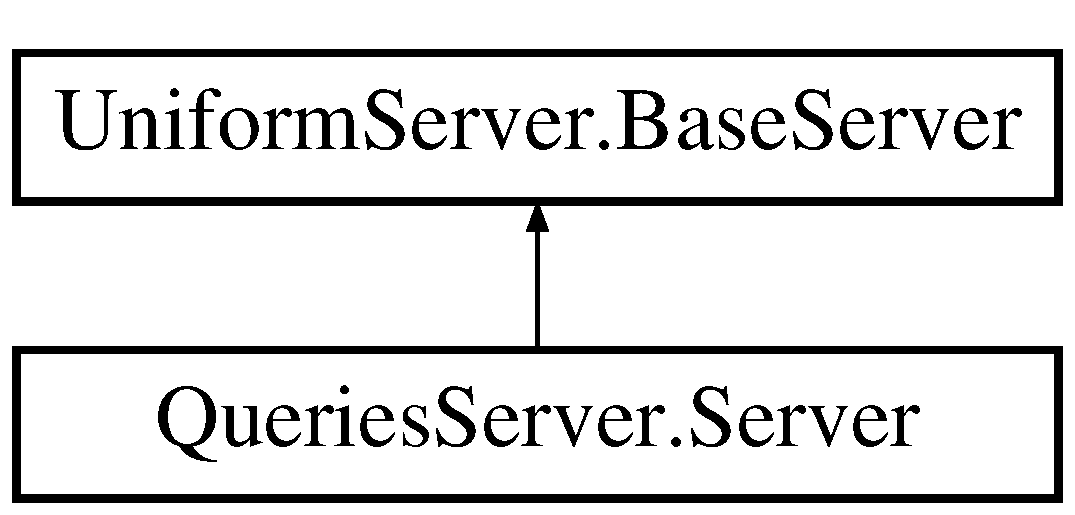
\includegraphics[height=2.000000cm]{d2/d9a/class_queries_server_1_1_server}
\end{center}
\end{figure}
\subsection*{Static Public Attributes}
\begin{DoxyCompactItemize}
\item 
static string \mbox{\hyperlink{class_queries_server_1_1_server_a5d7c4c9ababa7292ef7cac92005d3563}{O\+P\+E\+N\+\_\+\+C\+H\+A\+N\+EL}} = \char`\"{}T\+H\+B\+\_\+\+Q\+U\+E\+R\+Y\+\_\+\+S\+E\+R\+V\+ER\char`\"{}
\begin{DoxyCompactList}\small\item\em Main public pipe that will listen queries. \end{DoxyCompactList}\end{DoxyCompactItemize}
\subsection*{Static Private Member Functions}
\begin{DoxyCompactItemize}
\item 
static void \mbox{\hyperlink{class_queries_server_1_1_server_ae294b75511557ef0701455c0e2ba785d}{Main}} (string\mbox{[}$\,$\mbox{]} args)
\end{DoxyCompactItemize}
\subsection*{Additional Inherited Members}


\subsection{Detailed Description}
Public servers that allow anonimous connection. Reciving clients\textquotesingle{} queries and redirect in to target infrastructure servers by the comutation table. Reciving answer from servers and redirect it to target clients. 



\subsection{Member Function Documentation}
\mbox{\Hypertarget{class_queries_server_1_1_server_ae294b75511557ef0701455c0e2ba785d}\label{class_queries_server_1_1_server_ae294b75511557ef0701455c0e2ba785d}} 
\index{Queries\+Server\+::\+Server@{Queries\+Server\+::\+Server}!Main@{Main}}
\index{Main@{Main}!Queries\+Server\+::\+Server@{Queries\+Server\+::\+Server}}
\subsubsection{\texorpdfstring{Main()}{Main()}}
{\footnotesize\ttfamily static void Queries\+Server.\+Server.\+Main (\begin{DoxyParamCaption}\item[{string \mbox{[}$\,$\mbox{]}}]{args }\end{DoxyParamCaption})\hspace{0.3cm}{\ttfamily [static]}, {\ttfamily [private]}}

Draw line

Show help. 

\subsection{Member Data Documentation}
\mbox{\Hypertarget{class_queries_server_1_1_server_a5d7c4c9ababa7292ef7cac92005d3563}\label{class_queries_server_1_1_server_a5d7c4c9ababa7292ef7cac92005d3563}} 
\index{Queries\+Server\+::\+Server@{Queries\+Server\+::\+Server}!O\+P\+E\+N\+\_\+\+C\+H\+A\+N\+EL@{O\+P\+E\+N\+\_\+\+C\+H\+A\+N\+EL}}
\index{O\+P\+E\+N\+\_\+\+C\+H\+A\+N\+EL@{O\+P\+E\+N\+\_\+\+C\+H\+A\+N\+EL}!Queries\+Server\+::\+Server@{Queries\+Server\+::\+Server}}
\subsubsection{\texorpdfstring{O\+P\+E\+N\+\_\+\+C\+H\+A\+N\+EL}{OPEN\_CHANEL}}
{\footnotesize\ttfamily string Queries\+Server.\+Server.\+O\+P\+E\+N\+\_\+\+C\+H\+A\+N\+EL = \char`\"{}T\+H\+B\+\_\+\+Q\+U\+E\+R\+Y\+\_\+\+S\+E\+R\+V\+ER\char`\"{}\hspace{0.3cm}{\ttfamily [static]}}



Main public pipe that will listen queries. 



The documentation for this class was generated from the following file\+:\begin{DoxyCompactItemize}
\item 
D\+:/\+Work/\+Git\+Hub/doloro-\/networking-\/framework/\+Examples/\+Servers/\+Queries\+Server/Server.\+cs\end{DoxyCompactItemize}

\hypertarget{class_session_provider_1_1_server}{}\section{Session\+Provider.\+Server Class Reference}
\label{class_session_provider_1_1_server}\index{Session\+Provider.\+Server@{Session\+Provider.\+Server}}


\mbox{\hyperlink{class_session_provider_1_1_server}{Server}} tasks\+:  


Inheritance diagram for Session\+Provider.\+Server\+:\begin{figure}[H]
\begin{center}
\leavevmode
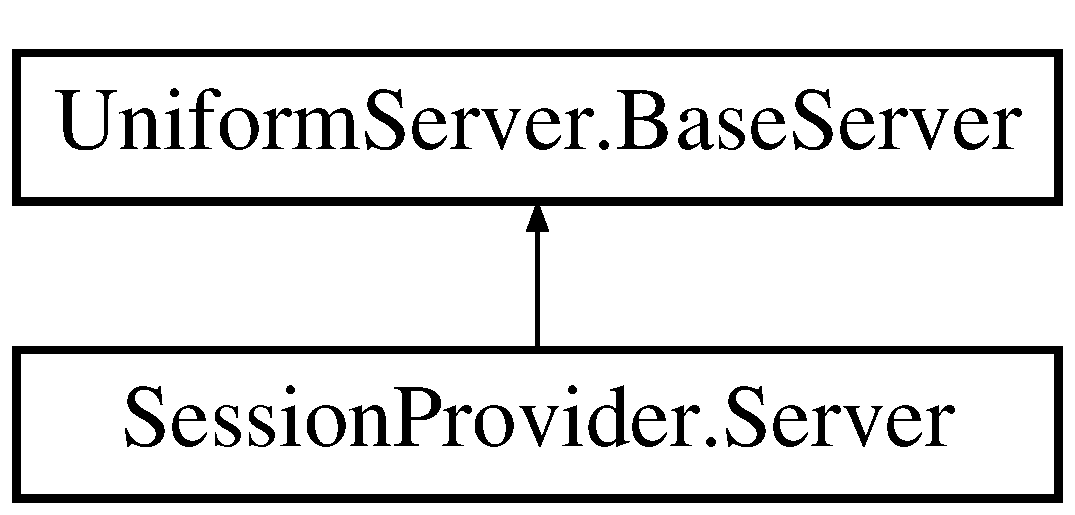
\includegraphics[height=2.000000cm]{d8/d17/class_session_provider_1_1_server}
\end{center}
\end{figure}
\subsection*{Properties}
\begin{DoxyCompactItemize}
\item 
\mbox{\Hypertarget{class_session_provider_1_1_server_a7ccb7c8e5465c2778d961034fcd6ac6f}\label{class_session_provider_1_1_server_a7ccb7c8e5465c2778d961034fcd6ac6f}} 
static bool {\bfseries Users\+Loaded}\hspace{0.3cm}{\ttfamily  \mbox{[}get, private set\mbox{]}}
\end{DoxyCompactItemize}
\subsection*{Static Private Member Functions}
\begin{DoxyCompactItemize}
\item 
static void \mbox{\hyperlink{class_session_provider_1_1_server_a78068e966b78f7579b01ba80f53b87ea}{Main}} (string\mbox{[}$\,$\mbox{]} args)
\item 
\mbox{\Hypertarget{class_session_provider_1_1_server_ad75d498e5203fe80a725f54ec955ace2}\label{class_session_provider_1_1_server_ad75d498e5203fe80a725f54ec955ace2}} 
static void {\bfseries Users\+\_\+\+Directory\+Loading\+Unlocked} (string unlocked\+Directory, int sucess, int failed)
\end{DoxyCompactItemize}
\subsection*{Additional Inherited Members}


\subsection{Detailed Description}
\mbox{\hyperlink{class_session_provider_1_1_server}{Server}} tasks\+: 


\begin{DoxyItemize}
\item Provide session token to clients.
\item User data managment.
\item Control rights. 
\end{DoxyItemize}

\subsection{Member Function Documentation}
\mbox{\Hypertarget{class_session_provider_1_1_server_a78068e966b78f7579b01ba80f53b87ea}\label{class_session_provider_1_1_server_a78068e966b78f7579b01ba80f53b87ea}} 
\index{Session\+Provider\+::\+Server@{Session\+Provider\+::\+Server}!Main@{Main}}
\index{Main@{Main}!Session\+Provider\+::\+Server@{Session\+Provider\+::\+Server}}
\subsubsection{\texorpdfstring{Main()}{Main()}}
{\footnotesize\ttfamily static void Session\+Provider.\+Server.\+Main (\begin{DoxyParamCaption}\item[{string \mbox{[}$\,$\mbox{]}}]{args }\end{DoxyParamCaption})\hspace{0.3cm}{\ttfamily [static]}, {\ttfamily [private]}}

Show help. 

The documentation for this class was generated from the following file\+:\begin{DoxyCompactItemize}
\item 
D\+:/\+Work/\+Git\+Hub/doloro-\/networking-\/framework/\+Examples/\+Servers/\+Session\+Provider/Server.\+cs\end{DoxyCompactItemize}

\hypertarget{class_pipes_provider_1_1_server_1_1_server_a_p_i}{}\section{Pipes\+Provider.\+Server.\+Server\+A\+PI Class Reference}
\label{class_pipes_provider_1_1_server_1_1_server_a_p_i}\index{Pipes\+Provider.\+Server.\+Server\+A\+PI@{Pipes\+Provider.\+Server.\+Server\+A\+PI}}


Class that provide common methods for easy work with pipes\textquotesingle{} tasks.  


\subsection*{Static Public Member Functions}
\begin{DoxyCompactItemize}
\item 
static void \mbox{\hyperlink{class_pipes_provider_1_1_server_1_1_server_a_p_i_aaf9afb864cf452d3842f0a6546569a32}{Server\+Loop$<$ Transmission\+Controller\+Type $>$}} (string guid, System.\+Action$<$ \mbox{\hyperlink{class_pipes_provider_1_1_server_1_1_transmission_controllers_1_1_base_server_transmission_controller}{Base\+Server\+Transmission\+Controller}} $>$ connection\+Callback, string pipe\+Name, Pipe\+Direction pipe\+Direction, int allowed\+Server\+Instances, Pipe\+Transmission\+Mode transmission\+Mode, Pipe\+Options pipe\+Options, \mbox{\hyperlink{namespace_pipes_provider_1_1_security_a1a6020eca1c661a6f7140e8260502d7e}{Security.\+Security\+Level}} security\+Level, System.\+Action$<$ \mbox{\hyperlink{class_pipes_provider_1_1_server_1_1_transmission_controllers_1_1_base_server_transmission_controller}{Base\+Server\+Transmission\+Controller}} $>$init\+Handler=null)
\begin{DoxyCompactList}\small\item\em Provide base server loop that control pipe. Have ability to full controll all handlers. \end{DoxyCompactList}\item 
static void \mbox{\hyperlink{class_pipes_provider_1_1_server_1_1_server_a_p_i_a750e3c4f0e34e61724ab3914d0d0608e}{Set\+Expired}} (string pipe\+Name)
\begin{DoxyCompactList}\small\item\em Marking pipe as expired. On the next loop tick connections will be disconnect and pipe will close. \end{DoxyCompactList}\item 
static void \mbox{\hyperlink{class_pipes_provider_1_1_server_1_1_server_a_p_i_a9adcab99d6a6b7e4185203afb74dc575}{Set\+Expired}} (\mbox{\hyperlink{class_pipes_provider_1_1_server_1_1_transmission_controllers_1_1_base_server_transmission_controller}{Base\+Server\+Transmission\+Controller}} meta)
\begin{DoxyCompactList}\small\item\em Marking pipe as expired. On the next loop tick connections will be disconnect and pipe will close. \end{DoxyCompactList}\item 
static void \mbox{\hyperlink{class_pipes_provider_1_1_server_1_1_server_a_p_i_a6d6f42c39e7f5c8a63a026739fe0ea94}{Set\+Expired\+All}} ()
\begin{DoxyCompactList}\small\item\em Markin all pipes as expired. Connection will be terminated. \end{DoxyCompactList}\item 
static void \mbox{\hyperlink{class_pipes_provider_1_1_server_1_1_server_a_p_i_af9c612e584b125b1fdc2c32490613bb1}{Stop\+Server}} (string pipe\+Name)
\begin{DoxyCompactList}\small\item\em Stop server by pipe name. \end{DoxyCompactList}\item 
static void \mbox{\hyperlink{class_pipes_provider_1_1_server_1_1_server_a_p_i_a8a70cec80dfb54ff68d8c4924a8b4007}{Stop\+Server}} (\mbox{\hyperlink{class_pipes_provider_1_1_server_1_1_transmission_controllers_1_1_base_server_transmission_controller}{Base\+Server\+Transmission\+Controller}} meta)
\begin{DoxyCompactList}\small\item\em Stop server by relative meta data. \end{DoxyCompactList}\item 
static void \mbox{\hyperlink{class_pipes_provider_1_1_server_1_1_server_a_p_i_a44469667416cb072d8fd258b299a53cd}{Stop\+All\+Servers}} ()
\begin{DoxyCompactList}\small\item\em Stoping all regirated servers. \end{DoxyCompactList}\item 
static bool \mbox{\hyperlink{class_pipes_provider_1_1_server_1_1_server_a_p_i_a6fba1adf18ce5938c6edcb29f28adfe5}{Try\+Get\+Server\+Transmission\+Controller}} (string guid, out \mbox{\hyperlink{class_pipes_provider_1_1_server_1_1_transmission_controllers_1_1_base_server_transmission_controller}{Base\+Server\+Transmission\+Controller}} meta)
\begin{DoxyCompactList}\small\item\em Try to find opened servert to client transmisssion meta data in common table. \end{DoxyCompactList}\end{DoxyCompactItemize}
\subsection*{Events}
\begin{DoxyCompactItemize}
\item 
static System.\+Action$<$ \mbox{\hyperlink{class_pipes_provider_1_1_server_1_1_transmission_controllers_1_1_base_server_transmission_controller}{Base\+Server\+Transmission\+Controller}} $>$ \mbox{\hyperlink{class_pipes_provider_1_1_server_1_1_server_a_p_i_adf4c77f25cd481b8190240e4aca06e56}{Server\+Transmission\+Meta\+\_\+\+In\+Processing}}
\begin{DoxyCompactList}\small\item\em Event that will be called when server transmission will be registred or updated. \end{DoxyCompactList}\end{DoxyCompactItemize}
\subsection*{Static Private Attributes}
\begin{DoxyCompactItemize}
\item 
static readonly Hashtable \mbox{\hyperlink{class_pipes_provider_1_1_server_1_1_server_a_p_i_ac18f0fca4de6269edeb97379112e67ca}{opened\+Servers}} = new Hashtable()
\begin{DoxyCompactList}\small\item\em Hashtable thast contain references to oppened pipes. Key (string) pipe\+\_\+name; Value (Server\+Transmission\+Meta) meta data about transmition. \end{DoxyCompactList}\end{DoxyCompactItemize}


\subsection{Detailed Description}
Class that provide common methods for easy work with pipes\textquotesingle{} tasks. 



\subsection{Member Function Documentation}
\mbox{\Hypertarget{class_pipes_provider_1_1_server_1_1_server_a_p_i_aaf9afb864cf452d3842f0a6546569a32}\label{class_pipes_provider_1_1_server_1_1_server_a_p_i_aaf9afb864cf452d3842f0a6546569a32}} 
\index{Pipes\+Provider\+::\+Server\+::\+Server\+A\+PI@{Pipes\+Provider\+::\+Server\+::\+Server\+A\+PI}!Server\+Loop$<$ Transmission\+Controller\+Type $>$@{Server\+Loop$<$ Transmission\+Controller\+Type $>$}}
\index{Server\+Loop$<$ Transmission\+Controller\+Type $>$@{Server\+Loop$<$ Transmission\+Controller\+Type $>$}!Pipes\+Provider\+::\+Server\+::\+Server\+A\+PI@{Pipes\+Provider\+::\+Server\+::\+Server\+A\+PI}}
\subsubsection{\texorpdfstring{Server\+Loop$<$ Transmission\+Controller\+Type $>$()}{ServerLoop< TransmissionControllerType >()}}
{\footnotesize\ttfamily static void Pipes\+Provider.\+Server.\+Server\+A\+P\+I.\+Server\+Loop$<$ Transmission\+Controller\+Type $>$ (\begin{DoxyParamCaption}\item[{string}]{guid,  }\item[{System.\+Action$<$ \mbox{\hyperlink{class_pipes_provider_1_1_server_1_1_transmission_controllers_1_1_base_server_transmission_controller}{Base\+Server\+Transmission\+Controller}} $>$}]{connection\+Callback,  }\item[{string}]{pipe\+Name,  }\item[{Pipe\+Direction}]{pipe\+Direction,  }\item[{int}]{allowed\+Server\+Instances,  }\item[{Pipe\+Transmission\+Mode}]{transmission\+Mode,  }\item[{Pipe\+Options}]{pipe\+Options,  }\item[{\mbox{\hyperlink{namespace_pipes_provider_1_1_security_a1a6020eca1c661a6f7140e8260502d7e}{Security.\+Security\+Level}}}]{security\+Level,  }\item[{System.\+Action$<$ \mbox{\hyperlink{class_pipes_provider_1_1_server_1_1_transmission_controllers_1_1_base_server_transmission_controller}{Base\+Server\+Transmission\+Controller}} $>$}]{init\+Handler = {\ttfamily null} }\end{DoxyParamCaption})\hspace{0.3cm}{\ttfamily [static]}}



Provide base server loop that control pipe. Have ability to full controll all handlers. 

Warrning\+: Use only if undersend how it work. Overwise use simplived Client\+To\+Server\+Loop or Server\+To\+Client\+Loop 


\begin{DoxyParams}{Parameters}
{\em connection\+Callback} & Delegate that will be called when connection will be established.\\
\hline
{\em pipe\+Name} & Name of pipe that will be used to acces by client.\\
\hline
{\em pipe\+Direction} & Dirrection of the possible transmission.\\
\hline
{\em allowed\+Server\+Instances} & How many server pipes can be started with the same name.\\
\hline
{\em transmission\+Mode} & Type of transmission.\\
\hline
{\em pipe\+Options} & Configuration of the pipe.\\
\hline
{\em init\+Handler} & Handler that will be called in case if transmisssion still not registred. Provide possibility to castom initialization for every type of controller.\\
\hline
\end{DoxyParams}
Update data. \begin{Desc}
\item[Type Constraints]\begin{description}
\item[{\em Transmission\+Controller\+Type} : {\em Base\+Server\+Transmission\+Controller}]\end{description}
\end{Desc}
\mbox{\Hypertarget{class_pipes_provider_1_1_server_1_1_server_a_p_i_a750e3c4f0e34e61724ab3914d0d0608e}\label{class_pipes_provider_1_1_server_1_1_server_a_p_i_a750e3c4f0e34e61724ab3914d0d0608e}} 
\index{Pipes\+Provider\+::\+Server\+::\+Server\+A\+PI@{Pipes\+Provider\+::\+Server\+::\+Server\+A\+PI}!Set\+Expired@{Set\+Expired}}
\index{Set\+Expired@{Set\+Expired}!Pipes\+Provider\+::\+Server\+::\+Server\+A\+PI@{Pipes\+Provider\+::\+Server\+::\+Server\+A\+PI}}
\subsubsection{\texorpdfstring{Set\+Expired()}{SetExpired()}\hspace{0.1cm}{\footnotesize\ttfamily [1/2]}}
{\footnotesize\ttfamily static void Pipes\+Provider.\+Server.\+Server\+A\+P\+I.\+Set\+Expired (\begin{DoxyParamCaption}\item[{string}]{pipe\+Name }\end{DoxyParamCaption})\hspace{0.3cm}{\ttfamily [static]}}



Marking pipe as expired. On the next loop tick connections will be disconnect and pipe will close. 


\begin{DoxyParams}{Parameters}
{\em pipe\+Name} & \\
\hline
\end{DoxyParams}
\mbox{\Hypertarget{class_pipes_provider_1_1_server_1_1_server_a_p_i_a9adcab99d6a6b7e4185203afb74dc575}\label{class_pipes_provider_1_1_server_1_1_server_a_p_i_a9adcab99d6a6b7e4185203afb74dc575}} 
\index{Pipes\+Provider\+::\+Server\+::\+Server\+A\+PI@{Pipes\+Provider\+::\+Server\+::\+Server\+A\+PI}!Set\+Expired@{Set\+Expired}}
\index{Set\+Expired@{Set\+Expired}!Pipes\+Provider\+::\+Server\+::\+Server\+A\+PI@{Pipes\+Provider\+::\+Server\+::\+Server\+A\+PI}}
\subsubsection{\texorpdfstring{Set\+Expired()}{SetExpired()}\hspace{0.1cm}{\footnotesize\ttfamily [2/2]}}
{\footnotesize\ttfamily static void Pipes\+Provider.\+Server.\+Server\+A\+P\+I.\+Set\+Expired (\begin{DoxyParamCaption}\item[{\mbox{\hyperlink{class_pipes_provider_1_1_server_1_1_transmission_controllers_1_1_base_server_transmission_controller}{Base\+Server\+Transmission\+Controller}}}]{meta }\end{DoxyParamCaption})\hspace{0.3cm}{\ttfamily [static]}}



Marking pipe as expired. On the next loop tick connections will be disconnect and pipe will close. 


\begin{DoxyParams}{Parameters}
{\em pipe\+Name} & \\
\hline
\end{DoxyParams}
\mbox{\Hypertarget{class_pipes_provider_1_1_server_1_1_server_a_p_i_a6d6f42c39e7f5c8a63a026739fe0ea94}\label{class_pipes_provider_1_1_server_1_1_server_a_p_i_a6d6f42c39e7f5c8a63a026739fe0ea94}} 
\index{Pipes\+Provider\+::\+Server\+::\+Server\+A\+PI@{Pipes\+Provider\+::\+Server\+::\+Server\+A\+PI}!Set\+Expired\+All@{Set\+Expired\+All}}
\index{Set\+Expired\+All@{Set\+Expired\+All}!Pipes\+Provider\+::\+Server\+::\+Server\+A\+PI@{Pipes\+Provider\+::\+Server\+::\+Server\+A\+PI}}
\subsubsection{\texorpdfstring{Set\+Expired\+All()}{SetExpiredAll()}}
{\footnotesize\ttfamily static void Pipes\+Provider.\+Server.\+Server\+A\+P\+I.\+Set\+Expired\+All (\begin{DoxyParamCaption}{ }\end{DoxyParamCaption})\hspace{0.3cm}{\ttfamily [static]}}



Markin all pipes as expired. Connection will be terminated. 

\mbox{\Hypertarget{class_pipes_provider_1_1_server_1_1_server_a_p_i_a44469667416cb072d8fd258b299a53cd}\label{class_pipes_provider_1_1_server_1_1_server_a_p_i_a44469667416cb072d8fd258b299a53cd}} 
\index{Pipes\+Provider\+::\+Server\+::\+Server\+A\+PI@{Pipes\+Provider\+::\+Server\+::\+Server\+A\+PI}!Stop\+All\+Servers@{Stop\+All\+Servers}}
\index{Stop\+All\+Servers@{Stop\+All\+Servers}!Pipes\+Provider\+::\+Server\+::\+Server\+A\+PI@{Pipes\+Provider\+::\+Server\+::\+Server\+A\+PI}}
\subsubsection{\texorpdfstring{Stop\+All\+Servers()}{StopAllServers()}}
{\footnotesize\ttfamily static void Pipes\+Provider.\+Server.\+Server\+A\+P\+I.\+Stop\+All\+Servers (\begin{DoxyParamCaption}{ }\end{DoxyParamCaption})\hspace{0.3cm}{\ttfamily [static]}}



Stoping all regirated servers. 

\mbox{\Hypertarget{class_pipes_provider_1_1_server_1_1_server_a_p_i_af9c612e584b125b1fdc2c32490613bb1}\label{class_pipes_provider_1_1_server_1_1_server_a_p_i_af9c612e584b125b1fdc2c32490613bb1}} 
\index{Pipes\+Provider\+::\+Server\+::\+Server\+A\+PI@{Pipes\+Provider\+::\+Server\+::\+Server\+A\+PI}!Stop\+Server@{Stop\+Server}}
\index{Stop\+Server@{Stop\+Server}!Pipes\+Provider\+::\+Server\+::\+Server\+A\+PI@{Pipes\+Provider\+::\+Server\+::\+Server\+A\+PI}}
\subsubsection{\texorpdfstring{Stop\+Server()}{StopServer()}\hspace{0.1cm}{\footnotesize\ttfamily [1/2]}}
{\footnotesize\ttfamily static void Pipes\+Provider.\+Server.\+Server\+A\+P\+I.\+Stop\+Server (\begin{DoxyParamCaption}\item[{string}]{pipe\+Name }\end{DoxyParamCaption})\hspace{0.3cm}{\ttfamily [static]}}



Stop server by pipe name. 


\begin{DoxyParams}{Parameters}
{\em pipe\+Name} & \\
\hline
\end{DoxyParams}
\mbox{\Hypertarget{class_pipes_provider_1_1_server_1_1_server_a_p_i_a8a70cec80dfb54ff68d8c4924a8b4007}\label{class_pipes_provider_1_1_server_1_1_server_a_p_i_a8a70cec80dfb54ff68d8c4924a8b4007}} 
\index{Pipes\+Provider\+::\+Server\+::\+Server\+A\+PI@{Pipes\+Provider\+::\+Server\+::\+Server\+A\+PI}!Stop\+Server@{Stop\+Server}}
\index{Stop\+Server@{Stop\+Server}!Pipes\+Provider\+::\+Server\+::\+Server\+A\+PI@{Pipes\+Provider\+::\+Server\+::\+Server\+A\+PI}}
\subsubsection{\texorpdfstring{Stop\+Server()}{StopServer()}\hspace{0.1cm}{\footnotesize\ttfamily [2/2]}}
{\footnotesize\ttfamily static void Pipes\+Provider.\+Server.\+Server\+A\+P\+I.\+Stop\+Server (\begin{DoxyParamCaption}\item[{\mbox{\hyperlink{class_pipes_provider_1_1_server_1_1_transmission_controllers_1_1_base_server_transmission_controller}{Base\+Server\+Transmission\+Controller}}}]{meta }\end{DoxyParamCaption})\hspace{0.3cm}{\ttfamily [static]}}



Stop server by relative meta data. 


\begin{DoxyParams}{Parameters}
{\em meta} & \\
\hline
\end{DoxyParams}
Log error. \mbox{\Hypertarget{class_pipes_provider_1_1_server_1_1_server_a_p_i_a6fba1adf18ce5938c6edcb29f28adfe5}\label{class_pipes_provider_1_1_server_1_1_server_a_p_i_a6fba1adf18ce5938c6edcb29f28adfe5}} 
\index{Pipes\+Provider\+::\+Server\+::\+Server\+A\+PI@{Pipes\+Provider\+::\+Server\+::\+Server\+A\+PI}!Try\+Get\+Server\+Transmission\+Controller@{Try\+Get\+Server\+Transmission\+Controller}}
\index{Try\+Get\+Server\+Transmission\+Controller@{Try\+Get\+Server\+Transmission\+Controller}!Pipes\+Provider\+::\+Server\+::\+Server\+A\+PI@{Pipes\+Provider\+::\+Server\+::\+Server\+A\+PI}}
\subsubsection{\texorpdfstring{Try\+Get\+Server\+Transmission\+Controller()}{TryGetServerTransmissionController()}}
{\footnotesize\ttfamily static bool Pipes\+Provider.\+Server.\+Server\+A\+P\+I.\+Try\+Get\+Server\+Transmission\+Controller (\begin{DoxyParamCaption}\item[{string}]{guid,  }\item[{out \mbox{\hyperlink{class_pipes_provider_1_1_server_1_1_transmission_controllers_1_1_base_server_transmission_controller}{Base\+Server\+Transmission\+Controller}}}]{meta }\end{DoxyParamCaption})\hspace{0.3cm}{\ttfamily [static]}}



Try to find opened servert to client transmisssion meta data in common table. 


\begin{DoxyParams}{Parameters}
{\em guid} & \\
\hline
{\em meta} & \\
\hline
\end{DoxyParams}
\begin{DoxyReturn}{Returns}

\end{DoxyReturn}


\subsection{Member Data Documentation}
\mbox{\Hypertarget{class_pipes_provider_1_1_server_1_1_server_a_p_i_ac18f0fca4de6269edeb97379112e67ca}\label{class_pipes_provider_1_1_server_1_1_server_a_p_i_ac18f0fca4de6269edeb97379112e67ca}} 
\index{Pipes\+Provider\+::\+Server\+::\+Server\+A\+PI@{Pipes\+Provider\+::\+Server\+::\+Server\+A\+PI}!opened\+Servers@{opened\+Servers}}
\index{opened\+Servers@{opened\+Servers}!Pipes\+Provider\+::\+Server\+::\+Server\+A\+PI@{Pipes\+Provider\+::\+Server\+::\+Server\+A\+PI}}
\subsubsection{\texorpdfstring{opened\+Servers}{openedServers}}
{\footnotesize\ttfamily readonly Hashtable Pipes\+Provider.\+Server.\+Server\+A\+P\+I.\+opened\+Servers = new Hashtable()\hspace{0.3cm}{\ttfamily [static]}, {\ttfamily [private]}}



Hashtable thast contain references to oppened pipes. Key (string) pipe\+\_\+name; Value (Server\+Transmission\+Meta) meta data about transmition. 



\subsection{Event Documentation}
\mbox{\Hypertarget{class_pipes_provider_1_1_server_1_1_server_a_p_i_adf4c77f25cd481b8190240e4aca06e56}\label{class_pipes_provider_1_1_server_1_1_server_a_p_i_adf4c77f25cd481b8190240e4aca06e56}} 
\index{Pipes\+Provider\+::\+Server\+::\+Server\+A\+PI@{Pipes\+Provider\+::\+Server\+::\+Server\+A\+PI}!Server\+Transmission\+Meta\+\_\+\+In\+Processing@{Server\+Transmission\+Meta\+\_\+\+In\+Processing}}
\index{Server\+Transmission\+Meta\+\_\+\+In\+Processing@{Server\+Transmission\+Meta\+\_\+\+In\+Processing}!Pipes\+Provider\+::\+Server\+::\+Server\+A\+PI@{Pipes\+Provider\+::\+Server\+::\+Server\+A\+PI}}
\subsubsection{\texorpdfstring{Server\+Transmission\+Meta\+\_\+\+In\+Processing}{ServerTransmissionMeta\_InProcessing}}
{\footnotesize\ttfamily System.\+Action$<$\mbox{\hyperlink{class_pipes_provider_1_1_server_1_1_transmission_controllers_1_1_base_server_transmission_controller}{Base\+Server\+Transmission\+Controller}}$>$ Pipes\+Provider.\+Server.\+Server\+A\+P\+I.\+Server\+Transmission\+Meta\+\_\+\+In\+Processing\hspace{0.3cm}{\ttfamily [static]}}



Event that will be called when server transmission will be registred or updated. 



The documentation for this class was generated from the following file\+:\begin{DoxyCompactItemize}
\item 
D\+:/\+Work/\+Git\+Hub/doloro-\/networking-\/framework/\+Pipes\+Provider/\+Server/Server\+A\+P\+I.\+cs\end{DoxyCompactItemize}

\hypertarget{class_pipes_provider_1_1_server_1_1_transmission_controllers_1_1_server_to_client_transmission_controller}{}\section{Pipes\+Provider.\+Server.\+Transmission\+Controllers.\+Server\+To\+Client\+Transmission\+Controller Class Reference}
\label{class_pipes_provider_1_1_server_1_1_transmission_controllers_1_1_server_to_client_transmission_controller}\index{Pipes\+Provider.\+Server.\+Transmission\+Controllers.\+Server\+To\+Client\+Transmission\+Controller@{Pipes\+Provider.\+Server.\+Transmission\+Controllers.\+Server\+To\+Client\+Transmission\+Controller}}


Controller that provide message\textquotesingle{}s transmisssion from server to client.  


Inheritance diagram for Pipes\+Provider.\+Server.\+Transmission\+Controllers.\+Server\+To\+Client\+Transmission\+Controller\+:\begin{figure}[H]
\begin{center}
\leavevmode
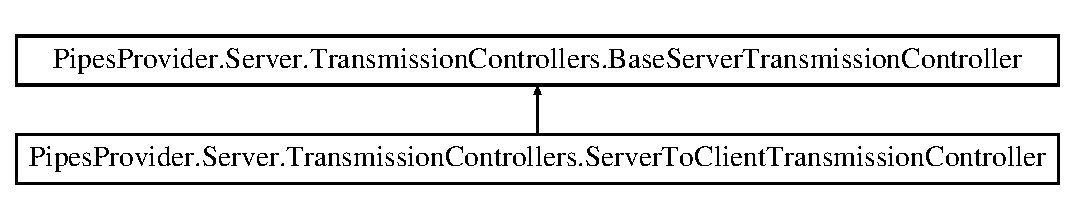
\includegraphics[height=2.000000cm]{d5/d4e/class_pipes_provider_1_1_server_1_1_transmission_controllers_1_1_server_to_client_transmission_controller}
\end{center}
\end{figure}
\subsection*{Public Member Functions}
\begin{DoxyCompactItemize}
\item 
\mbox{\Hypertarget{class_pipes_provider_1_1_server_1_1_transmission_controllers_1_1_server_to_client_transmission_controller_afa5595e45959941c7d3e84e868a25223}\label{class_pipes_provider_1_1_server_1_1_transmission_controllers_1_1_server_to_client_transmission_controller_afa5595e45959941c7d3e84e868a25223}} 
{\bfseries Server\+To\+Client\+Transmission\+Controller} (I\+Async\+Result \mbox{\hyperlink{class_pipes_provider_1_1_server_1_1_transmission_controllers_1_1_base_server_transmission_controller_afc45a2287e6fef24892a0aee8aa86f56}{connection\+Marker}}, System.\+Action$<$ \mbox{\hyperlink{class_pipes_provider_1_1_server_1_1_transmission_controllers_1_1_base_server_transmission_controller}{Base\+Server\+Transmission\+Controller}} $>$ \mbox{\hyperlink{class_pipes_provider_1_1_server_1_1_transmission_controllers_1_1_base_server_transmission_controller_a632261255d8dfc87d93445180c6e2c9d}{connection\+Callback}}, Named\+Pipe\+Server\+Stream pipe, string \mbox{\hyperlink{class_pipes_provider_1_1_server_1_1_transmission_controllers_1_1_base_server_transmission_controller_a4ce9911f1ad6814d3e5c9096d9ddde57}{pipe\+Name}})
\end{DoxyCompactItemize}
\subsection*{Static Public Member Functions}
\begin{DoxyCompactItemize}
\item 
static void \mbox{\hyperlink{class_pipes_provider_1_1_server_1_1_transmission_controllers_1_1_server_to_client_transmission_controller_a1315fe8071f9e83fdaae7d248cf822e2}{Server\+Loop}} (string \mbox{\hyperlink{class_pipes_provider_1_1_server_1_1_transmission_controllers_1_1_base_server_transmission_controller_a4ce9911f1ad6814d3e5c9096d9ddde57}{pipe\+Name}}, out string guid, \mbox{\hyperlink{namespace_pipes_provider_1_1_security_a1a6020eca1c661a6f7140e8260502d7e}{Security.\+Security\+Level}} security\+Level)
\begin{DoxyCompactList}\small\item\em Automaticly create server\textquotesingle{}s pipe that will send message to client. \end{DoxyCompactList}\item 
static void \mbox{\hyperlink{class_pipes_provider_1_1_server_1_1_transmission_controllers_1_1_server_to_client_transmission_controller_a0b40f93950cbf37335373f6efec0a4f1}{Server\+Loop}} (string guid, string \mbox{\hyperlink{class_pipes_provider_1_1_server_1_1_transmission_controllers_1_1_base_server_transmission_controller_a4ce9911f1ad6814d3e5c9096d9ddde57}{pipe\+Name}}, \mbox{\hyperlink{namespace_pipes_provider_1_1_security_a1a6020eca1c661a6f7140e8260502d7e}{Security.\+Security\+Level}} security\+Level)
\begin{DoxyCompactList}\small\item\em Automaticly create server\textquotesingle{}s pipe that will send message to client. \end{DoxyCompactList}\end{DoxyCompactItemize}
\subsection*{Properties}
\begin{DoxyCompactItemize}
\item 
string \mbox{\hyperlink{class_pipes_provider_1_1_server_1_1_transmission_controllers_1_1_server_to_client_transmission_controller_abc1b9e3483f9e0f1fd83e72d9b87377d}{Processing\+Query}}\hspace{0.3cm}{\ttfamily  \mbox{[}get, set\mbox{]}}
\begin{DoxyCompactList}\small\item\em Query that actualy in processing. \end{DoxyCompactList}\end{DoxyCompactItemize}
\subsection*{Additional Inherited Members}


\subsection{Detailed Description}
Controller that provide message\textquotesingle{}s transmisssion from server to client. 



\subsection{Member Function Documentation}
\mbox{\Hypertarget{class_pipes_provider_1_1_server_1_1_transmission_controllers_1_1_server_to_client_transmission_controller_a1315fe8071f9e83fdaae7d248cf822e2}\label{class_pipes_provider_1_1_server_1_1_transmission_controllers_1_1_server_to_client_transmission_controller_a1315fe8071f9e83fdaae7d248cf822e2}} 
\index{Pipes\+Provider\+::\+Server\+::\+Transmission\+Controllers\+::\+Server\+To\+Client\+Transmission\+Controller@{Pipes\+Provider\+::\+Server\+::\+Transmission\+Controllers\+::\+Server\+To\+Client\+Transmission\+Controller}!Server\+Loop@{Server\+Loop}}
\index{Server\+Loop@{Server\+Loop}!Pipes\+Provider\+::\+Server\+::\+Transmission\+Controllers\+::\+Server\+To\+Client\+Transmission\+Controller@{Pipes\+Provider\+::\+Server\+::\+Transmission\+Controllers\+::\+Server\+To\+Client\+Transmission\+Controller}}
\subsubsection{\texorpdfstring{Server\+Loop()}{ServerLoop()}\hspace{0.1cm}{\footnotesize\ttfamily [1/2]}}
{\footnotesize\ttfamily static void Pipes\+Provider.\+Server.\+Transmission\+Controllers.\+Server\+To\+Client\+Transmission\+Controller.\+Server\+Loop (\begin{DoxyParamCaption}\item[{string}]{pipe\+Name,  }\item[{out string}]{guid,  }\item[{\mbox{\hyperlink{namespace_pipes_provider_1_1_security_a1a6020eca1c661a6f7140e8260502d7e}{Security.\+Security\+Level}}}]{security\+Level }\end{DoxyParamCaption})\hspace{0.3cm}{\ttfamily [static]}}



Automaticly create server\textquotesingle{}s pipe that will send message to client. 


\begin{DoxyParams}{Parameters}
{\em query\+Handler\+Callback} & Callback that will be called when server will recive query from clinet.\\
\hline
{\em pipe\+Name} & Name of pipe that will created. \mbox{\hyperlink{namespace_pipes_provider_1_1_client}{Client}} will access this server using that name.\\
\hline
\end{DoxyParams}
\mbox{\Hypertarget{class_pipes_provider_1_1_server_1_1_transmission_controllers_1_1_server_to_client_transmission_controller_a0b40f93950cbf37335373f6efec0a4f1}\label{class_pipes_provider_1_1_server_1_1_transmission_controllers_1_1_server_to_client_transmission_controller_a0b40f93950cbf37335373f6efec0a4f1}} 
\index{Pipes\+Provider\+::\+Server\+::\+Transmission\+Controllers\+::\+Server\+To\+Client\+Transmission\+Controller@{Pipes\+Provider\+::\+Server\+::\+Transmission\+Controllers\+::\+Server\+To\+Client\+Transmission\+Controller}!Server\+Loop@{Server\+Loop}}
\index{Server\+Loop@{Server\+Loop}!Pipes\+Provider\+::\+Server\+::\+Transmission\+Controllers\+::\+Server\+To\+Client\+Transmission\+Controller@{Pipes\+Provider\+::\+Server\+::\+Transmission\+Controllers\+::\+Server\+To\+Client\+Transmission\+Controller}}
\subsubsection{\texorpdfstring{Server\+Loop()}{ServerLoop()}\hspace{0.1cm}{\footnotesize\ttfamily [2/2]}}
{\footnotesize\ttfamily static void Pipes\+Provider.\+Server.\+Transmission\+Controllers.\+Server\+To\+Client\+Transmission\+Controller.\+Server\+Loop (\begin{DoxyParamCaption}\item[{string}]{guid,  }\item[{string}]{pipe\+Name,  }\item[{\mbox{\hyperlink{namespace_pipes_provider_1_1_security_a1a6020eca1c661a6f7140e8260502d7e}{Security.\+Security\+Level}}}]{security\+Level }\end{DoxyParamCaption})\hspace{0.3cm}{\ttfamily [static]}}



Automaticly create server\textquotesingle{}s pipe that will send message to client. 


\begin{DoxyParams}{Parameters}
{\em query\+Handler\+Callback} & Callback that will be called when server will recive query from clinet.\\
\hline
{\em pipe\+Name} & Name of pipe that will created. \mbox{\hyperlink{namespace_pipes_provider_1_1_client}{Client}} will access this server using that name.\\
\hline
\end{DoxyParams}


\subsection{Property Documentation}
\mbox{\Hypertarget{class_pipes_provider_1_1_server_1_1_transmission_controllers_1_1_server_to_client_transmission_controller_abc1b9e3483f9e0f1fd83e72d9b87377d}\label{class_pipes_provider_1_1_server_1_1_transmission_controllers_1_1_server_to_client_transmission_controller_abc1b9e3483f9e0f1fd83e72d9b87377d}} 
\index{Pipes\+Provider\+::\+Server\+::\+Transmission\+Controllers\+::\+Server\+To\+Client\+Transmission\+Controller@{Pipes\+Provider\+::\+Server\+::\+Transmission\+Controllers\+::\+Server\+To\+Client\+Transmission\+Controller}!Processing\+Query@{Processing\+Query}}
\index{Processing\+Query@{Processing\+Query}!Pipes\+Provider\+::\+Server\+::\+Transmission\+Controllers\+::\+Server\+To\+Client\+Transmission\+Controller@{Pipes\+Provider\+::\+Server\+::\+Transmission\+Controllers\+::\+Server\+To\+Client\+Transmission\+Controller}}
\subsubsection{\texorpdfstring{Processing\+Query}{ProcessingQuery}}
{\footnotesize\ttfamily string Pipes\+Provider.\+Server.\+Transmission\+Controllers.\+Server\+To\+Client\+Transmission\+Controller.\+Processing\+Query\hspace{0.3cm}{\ttfamily [get]}, {\ttfamily [set]}}



Query that actualy in processing. 

Attention\+: Value can be changed if some of handlers will call disconecction or transmission error. This situation will lead to establishing new connection that lead to changing of this value. 

The documentation for this class was generated from the following file\+:\begin{DoxyCompactItemize}
\item 
D\+:/\+Work/\+Git\+Hub/doloro-\/networking-\/framework/\+Pipes\+Provider/\+Server/\+Transmisssion\+Controllers/Server\+To\+Client\+Transmission\+Controller.\+cs\end{DoxyCompactItemize}

\hypertarget{class_pipes_provider_1_1_handlers_1_1_service}{}\section{Pipes\+Provider.\+Handlers.\+Service Class Reference}
\label{class_pipes_provider_1_1_handlers_1_1_service}\index{Pipes\+Provider.\+Handlers.\+Service@{Pipes\+Provider.\+Handlers.\+Service}}


\mbox{\hyperlink{class_pipes_provider_1_1_handlers_1_1_service}{Service}} handlers that provide core processing and stability.  


\subsection*{Static Public Member Functions}
\begin{DoxyCompactItemize}
\item 
static async void \mbox{\hyperlink{class_pipes_provider_1_1_handlers_1_1_service_af208afd61f2abcb7ff163e5c2c6d81c9}{Connection\+Established\+Callback\+Retranslator}} (I\+Async\+Result result)
\begin{DoxyCompactList}\small\item\em Callback that will react on connection esstablishing. Will close waiting async operation and call shared delegate with server loop\textquotesingle{}s code. \end{DoxyCompactList}\end{DoxyCompactItemize}


\subsection{Detailed Description}
\mbox{\hyperlink{class_pipes_provider_1_1_handlers_1_1_service}{Service}} handlers that provide core processing and stability. 



\subsection{Member Function Documentation}
\mbox{\Hypertarget{class_pipes_provider_1_1_handlers_1_1_service_af208afd61f2abcb7ff163e5c2c6d81c9}\label{class_pipes_provider_1_1_handlers_1_1_service_af208afd61f2abcb7ff163e5c2c6d81c9}} 
\index{Pipes\+Provider\+::\+Handlers\+::\+Service@{Pipes\+Provider\+::\+Handlers\+::\+Service}!Connection\+Established\+Callback\+Retranslator@{Connection\+Established\+Callback\+Retranslator}}
\index{Connection\+Established\+Callback\+Retranslator@{Connection\+Established\+Callback\+Retranslator}!Pipes\+Provider\+::\+Handlers\+::\+Service@{Pipes\+Provider\+::\+Handlers\+::\+Service}}
\subsubsection{\texorpdfstring{Connection\+Established\+Callback\+Retranslator()}{ConnectionEstablishedCallbackRetranslator()}}
{\footnotesize\ttfamily static async void Pipes\+Provider.\+Handlers.\+Service.\+Connection\+Established\+Callback\+Retranslator (\begin{DoxyParamCaption}\item[{I\+Async\+Result}]{result }\end{DoxyParamCaption})\hspace{0.3cm}{\ttfamily [static]}}



Callback that will react on connection esstablishing. Will close waiting async operation and call shared delegate with server loop\textquotesingle{}s code. 


\begin{DoxyParams}{Parameters}
{\em result} & \\
\hline
\end{DoxyParams}


The documentation for this class was generated from the following file\+:\begin{DoxyCompactItemize}
\item 
D\+:/\+Work/\+Git\+Hub/doloro-\/networking-\/framework/\+Pipes\+Provider/\+Handlers/Service.\+cs\end{DoxyCompactItemize}

\hypertarget{class_authority_controller_1_1_session}{}\section{Authority\+Controller.\+Session Class Reference}
\label{class_authority_controller_1_1_session}\index{Authority\+Controller.\+Session@{Authority\+Controller.\+Session}}


Object that control data relative to current authority session.  


\subsection*{Public Member Functions}
\begin{DoxyCompactItemize}
\item 
bool \mbox{\hyperlink{class_authority_controller_1_1_session_a798dbdfeeb3ce9156d99d8b7962d9528}{Asign\+Token\+To\+User}} (\mbox{\hyperlink{class_authority_controller_1_1_data_1_1_user}{User}} user, string token)
\begin{DoxyCompactList}\small\item\em Create token registration binded for user profile. Not profided fields would filled like anonymous. Time stamp will contain the time of method call. \end{DoxyCompactList}\item 
bool \mbox{\hyperlink{class_authority_controller_1_1_session_ab164831d0a5fc909c200feba1ac882e4}{Asign\+Token\+To\+User}} (\mbox{\hyperlink{class_authority_controller_1_1_data_1_1_user}{User}} user, string token, string mac, string os, string stamp)
\begin{DoxyCompactList}\small\item\em Create token registration binded for user profile. \end{DoxyCompactList}\item 
void \mbox{\hyperlink{class_authority_controller_1_1_session_a481d888a9a2e90f1e43c60de7e1c7a71}{Set\+Token\+Rights}} (string token, params string\mbox{[}$\,$\mbox{]} rights)
\begin{DoxyCompactList}\small\item\em Set rights\textquotesingle{} codes array as relative to token. \end{DoxyCompactList}\item 
bool \mbox{\hyperlink{class_authority_controller_1_1_session_a37157e74e3aee082b7adfb906ec69511}{Try\+Get\+Token\+Rights}} (string token, out string\mbox{[}$\,$\mbox{]} rights)
\begin{DoxyCompactList}\small\item\em Trying to load rights registred for token. \end{DoxyCompactList}\item 
bool \mbox{\hyperlink{class_authority_controller_1_1_session_a811b23b70e61ac567ec8eeb54641ffcd}{Set\+Expired}} (string token)
\begin{DoxyCompactList}\small\item\em Removing of token from table and inform relative servers about that. \end{DoxyCompactList}\item 
bool \mbox{\hyperlink{class_authority_controller_1_1_session_abdd6c48f989b28cc9b3838dbe569edc6}{Try\+Get\+Token\+Info}} (string token, out \mbox{\hyperlink{class_authority_controller_1_1_data_1_1_token_info}{Token\+Info}} info)
\begin{DoxyCompactList}\small\item\em Try to find registred token info. \end{DoxyCompactList}\end{DoxyCompactItemize}
\subsection*{Properties}
\begin{DoxyCompactItemize}
\item 
static \mbox{\hyperlink{class_authority_controller_1_1_session}{Session}} \mbox{\hyperlink{class_authority_controller_1_1_session_a20d84345a3843b7a1b340887bb961f7c}{Current}}\hspace{0.3cm}{\ttfamily  \mbox{[}get, protected set\mbox{]}}
\begin{DoxyCompactList}\small\item\em Last created session. \end{DoxyCompactList}\end{DoxyCompactItemize}
\subsection*{Events}
\begin{DoxyCompactItemize}
\item 
static System.\+Action$<$ string $>$ \mbox{\hyperlink{class_authority_controller_1_1_session_abbd978421ebd42315bde41126231ac18}{Informate\+Related\+Servers}}
\begin{DoxyCompactList}\small\item\em Event that would called when provider would need to informate related servers by new data. \end{DoxyCompactList}\end{DoxyCompactItemize}
\subsection*{Private Member Functions}
\begin{DoxyCompactItemize}
\item 
bool \mbox{\hyperlink{class_authority_controller_1_1_session_a8422d53f01daff616c1588cb3d657882}{Remove\+Token}} (string token)
\begin{DoxyCompactList}\small\item\em Removing token from table. \end{DoxyCompactList}\item 
void \mbox{\hyperlink{class_authority_controller_1_1_session_ae8e875b83d01b42f4623d2c81841ce62}{Share\+Token\+Rights}} (string token, string\mbox{[}$\,$\mbox{]} rights)
\begin{DoxyCompactList}\small\item\em Sending new rights of token to related servers. \end{DoxyCompactList}\end{DoxyCompactItemize}
\subsection*{Private Attributes}
\begin{DoxyCompactItemize}
\item 
readonly Hashtable \mbox{\hyperlink{class_authority_controller_1_1_session_a69364ca8d68ac74a7220bdabb1551799}{tokens\+Rights}} = new Hashtable()
\begin{DoxyCompactList}\small\item\em Table that contains rights provided to token. \end{DoxyCompactList}\end{DoxyCompactItemize}
\subsection*{Static Private Attributes}
\begin{DoxyCompactItemize}
\item 
\mbox{\Hypertarget{class_authority_controller_1_1_session_a774ff0a1fec6aae096af9ed744c7269d}\label{class_authority_controller_1_1_session_a774ff0a1fec6aae096af9ed744c7269d}} 
static \mbox{\hyperlink{class_authority_controller_1_1_session}{Session}} \mbox{\hyperlink{class_authority_controller_1_1_session_a774ff0a1fec6aae096af9ed744c7269d}{last}}
\begin{DoxyCompactList}\small\item\em Object that contain current session. \end{DoxyCompactList}\end{DoxyCompactItemize}


\subsection{Detailed Description}
Object that control data relative to current authority session. 



\subsection{Member Function Documentation}
\mbox{\Hypertarget{class_authority_controller_1_1_session_a798dbdfeeb3ce9156d99d8b7962d9528}\label{class_authority_controller_1_1_session_a798dbdfeeb3ce9156d99d8b7962d9528}} 
\index{Authority\+Controller\+::\+Session@{Authority\+Controller\+::\+Session}!Asign\+Token\+To\+User@{Asign\+Token\+To\+User}}
\index{Asign\+Token\+To\+User@{Asign\+Token\+To\+User}!Authority\+Controller\+::\+Session@{Authority\+Controller\+::\+Session}}
\subsubsection{\texorpdfstring{Asign\+Token\+To\+User()}{AsignTokenToUser()}\hspace{0.1cm}{\footnotesize\ttfamily [1/2]}}
{\footnotesize\ttfamily bool Authority\+Controller.\+Session.\+Asign\+Token\+To\+User (\begin{DoxyParamCaption}\item[{\mbox{\hyperlink{class_authority_controller_1_1_data_1_1_user}{User}}}]{user,  }\item[{string}]{token }\end{DoxyParamCaption})}



Create token registration binded for user profile. Not profided fields would filled like anonymous. Time stamp will contain the time of method call. 


\begin{DoxyParams}{Parameters}
{\em user} & \\
\hline
{\em token} & \\
\hline
\end{DoxyParams}
\begin{DoxyReturn}{Returns}

\end{DoxyReturn}
\mbox{\Hypertarget{class_authority_controller_1_1_session_ab164831d0a5fc909c200feba1ac882e4}\label{class_authority_controller_1_1_session_ab164831d0a5fc909c200feba1ac882e4}} 
\index{Authority\+Controller\+::\+Session@{Authority\+Controller\+::\+Session}!Asign\+Token\+To\+User@{Asign\+Token\+To\+User}}
\index{Asign\+Token\+To\+User@{Asign\+Token\+To\+User}!Authority\+Controller\+::\+Session@{Authority\+Controller\+::\+Session}}
\subsubsection{\texorpdfstring{Asign\+Token\+To\+User()}{AsignTokenToUser()}\hspace{0.1cm}{\footnotesize\ttfamily [2/2]}}
{\footnotesize\ttfamily bool Authority\+Controller.\+Session.\+Asign\+Token\+To\+User (\begin{DoxyParamCaption}\item[{\mbox{\hyperlink{class_authority_controller_1_1_data_1_1_user}{User}}}]{user,  }\item[{string}]{token,  }\item[{string}]{mac,  }\item[{string}]{os,  }\item[{string}]{stamp }\end{DoxyParamCaption})}



Create token registration binded for user profile. 


\begin{DoxyParams}{Parameters}
{\em user} & User profile that contain core data.\\
\hline
{\em token} & Token provided to that user.\\
\hline
{\em mac} & Mac adress of user machine.\\
\hline
{\em os} & OS of user.\\
\hline
{\em stamp} & Time stamp that show when the session was started.\\
\hline
\end{DoxyParams}
\begin{DoxyReturn}{Returns}

\end{DoxyReturn}
\mbox{\Hypertarget{class_authority_controller_1_1_session_a8422d53f01daff616c1588cb3d657882}\label{class_authority_controller_1_1_session_a8422d53f01daff616c1588cb3d657882}} 
\index{Authority\+Controller\+::\+Session@{Authority\+Controller\+::\+Session}!Remove\+Token@{Remove\+Token}}
\index{Remove\+Token@{Remove\+Token}!Authority\+Controller\+::\+Session@{Authority\+Controller\+::\+Session}}
\subsubsection{\texorpdfstring{Remove\+Token()}{RemoveToken()}}
{\footnotesize\ttfamily bool Authority\+Controller.\+Session.\+Remove\+Token (\begin{DoxyParamCaption}\item[{string}]{token }\end{DoxyParamCaption})\hspace{0.3cm}{\ttfamily [private]}}



Removing token from table. 


\begin{DoxyParams}{Parameters}
{\em token} & \\
\hline
\end{DoxyParams}
\begin{DoxyReturn}{Returns}
Is removed successful?
\end{DoxyReturn}
\mbox{\Hypertarget{class_authority_controller_1_1_session_a811b23b70e61ac567ec8eeb54641ffcd}\label{class_authority_controller_1_1_session_a811b23b70e61ac567ec8eeb54641ffcd}} 
\index{Authority\+Controller\+::\+Session@{Authority\+Controller\+::\+Session}!Set\+Expired@{Set\+Expired}}
\index{Set\+Expired@{Set\+Expired}!Authority\+Controller\+::\+Session@{Authority\+Controller\+::\+Session}}
\subsubsection{\texorpdfstring{Set\+Expired()}{SetExpired()}}
{\footnotesize\ttfamily bool Authority\+Controller.\+Session.\+Set\+Expired (\begin{DoxyParamCaption}\item[{string}]{token }\end{DoxyParamCaption})}



Removing of token from table and inform relative servers about that. 


\begin{DoxyParams}{Parameters}
{\em token} & \\
\hline
\end{DoxyParams}
\mbox{\Hypertarget{class_authority_controller_1_1_session_a481d888a9a2e90f1e43c60de7e1c7a71}\label{class_authority_controller_1_1_session_a481d888a9a2e90f1e43c60de7e1c7a71}} 
\index{Authority\+Controller\+::\+Session@{Authority\+Controller\+::\+Session}!Set\+Token\+Rights@{Set\+Token\+Rights}}
\index{Set\+Token\+Rights@{Set\+Token\+Rights}!Authority\+Controller\+::\+Session@{Authority\+Controller\+::\+Session}}
\subsubsection{\texorpdfstring{Set\+Token\+Rights()}{SetTokenRights()}}
{\footnotesize\ttfamily void Authority\+Controller.\+Session.\+Set\+Token\+Rights (\begin{DoxyParamCaption}\item[{string}]{token,  }\item[{params string \mbox{[}$\,$\mbox{]}}]{rights }\end{DoxyParamCaption})}



Set rights\textquotesingle{} codes array as relative to token. 

In case if token infor not registred then will create anonimouse info with applied rights. Applicable to purposes of servers that depends to session provider one, but not require entire token information, cause not manage it. 


\begin{DoxyParams}{Parameters}
{\em token} & \mbox{\hyperlink{class_authority_controller_1_1_session}{Session}} token.\\
\hline
{\em rights} & Array og rights\textquotesingle{} codes.\\
\hline
\end{DoxyParams}
\mbox{\Hypertarget{class_authority_controller_1_1_session_ae8e875b83d01b42f4623d2c81841ce62}\label{class_authority_controller_1_1_session_ae8e875b83d01b42f4623d2c81841ce62}} 
\index{Authority\+Controller\+::\+Session@{Authority\+Controller\+::\+Session}!Share\+Token\+Rights@{Share\+Token\+Rights}}
\index{Share\+Token\+Rights@{Share\+Token\+Rights}!Authority\+Controller\+::\+Session@{Authority\+Controller\+::\+Session}}
\subsubsection{\texorpdfstring{Share\+Token\+Rights()}{ShareTokenRights()}}
{\footnotesize\ttfamily void Authority\+Controller.\+Session.\+Share\+Token\+Rights (\begin{DoxyParamCaption}\item[{string}]{token,  }\item[{string \mbox{[}$\,$\mbox{]}}]{rights }\end{DoxyParamCaption})\hspace{0.3cm}{\ttfamily [private]}}



Sending new rights of token to related servers. 


\begin{DoxyParams}{Parameters}
{\em token} & \\
\hline
{\em rights} & \\
\hline
\end{DoxyParams}
\mbox{\Hypertarget{class_authority_controller_1_1_session_abdd6c48f989b28cc9b3838dbe569edc6}\label{class_authority_controller_1_1_session_abdd6c48f989b28cc9b3838dbe569edc6}} 
\index{Authority\+Controller\+::\+Session@{Authority\+Controller\+::\+Session}!Try\+Get\+Token\+Info@{Try\+Get\+Token\+Info}}
\index{Try\+Get\+Token\+Info@{Try\+Get\+Token\+Info}!Authority\+Controller\+::\+Session@{Authority\+Controller\+::\+Session}}
\subsubsection{\texorpdfstring{Try\+Get\+Token\+Info()}{TryGetTokenInfo()}}
{\footnotesize\ttfamily bool Authority\+Controller.\+Session.\+Try\+Get\+Token\+Info (\begin{DoxyParamCaption}\item[{string}]{token,  }\item[{out \mbox{\hyperlink{class_authority_controller_1_1_data_1_1_token_info}{Token\+Info}}}]{info }\end{DoxyParamCaption})}



Try to find registred token info. 


\begin{DoxyParams}{Parameters}
{\em token} & \\
\hline
{\em info} & \\
\hline
\end{DoxyParams}
\begin{DoxyReturn}{Returns}

\end{DoxyReturn}
\mbox{\Hypertarget{class_authority_controller_1_1_session_a37157e74e3aee082b7adfb906ec69511}\label{class_authority_controller_1_1_session_a37157e74e3aee082b7adfb906ec69511}} 
\index{Authority\+Controller\+::\+Session@{Authority\+Controller\+::\+Session}!Try\+Get\+Token\+Rights@{Try\+Get\+Token\+Rights}}
\index{Try\+Get\+Token\+Rights@{Try\+Get\+Token\+Rights}!Authority\+Controller\+::\+Session@{Authority\+Controller\+::\+Session}}
\subsubsection{\texorpdfstring{Try\+Get\+Token\+Rights()}{TryGetTokenRights()}}
{\footnotesize\ttfamily bool Authority\+Controller.\+Session.\+Try\+Get\+Token\+Rights (\begin{DoxyParamCaption}\item[{string}]{token,  }\item[{out string \mbox{[}$\,$\mbox{]}}]{rights }\end{DoxyParamCaption})}



Trying to load rights registred for token. 


\begin{DoxyParams}{Parameters}
{\em token} & \mbox{\hyperlink{class_authority_controller_1_1_session}{Session}} token.\\
\hline
{\em rights} & Array of rights\textquotesingle{} codes relative to token.\\
\hline
\end{DoxyParams}
\begin{DoxyReturn}{Returns}

\end{DoxyReturn}


\subsection{Member Data Documentation}
\mbox{\Hypertarget{class_authority_controller_1_1_session_a69364ca8d68ac74a7220bdabb1551799}\label{class_authority_controller_1_1_session_a69364ca8d68ac74a7220bdabb1551799}} 
\index{Authority\+Controller\+::\+Session@{Authority\+Controller\+::\+Session}!tokens\+Rights@{tokens\+Rights}}
\index{tokens\+Rights@{tokens\+Rights}!Authority\+Controller\+::\+Session@{Authority\+Controller\+::\+Session}}
\subsubsection{\texorpdfstring{tokens\+Rights}{tokensRights}}
{\footnotesize\ttfamily readonly Hashtable Authority\+Controller.\+Session.\+tokens\+Rights = new Hashtable()\hspace{0.3cm}{\ttfamily [private]}}



Table that contains rights provided to token. 

Key -\/ string token Value -\/ Token\+Info 

\subsection{Property Documentation}
\mbox{\Hypertarget{class_authority_controller_1_1_session_a20d84345a3843b7a1b340887bb961f7c}\label{class_authority_controller_1_1_session_a20d84345a3843b7a1b340887bb961f7c}} 
\index{Authority\+Controller\+::\+Session@{Authority\+Controller\+::\+Session}!Current@{Current}}
\index{Current@{Current}!Authority\+Controller\+::\+Session@{Authority\+Controller\+::\+Session}}
\subsubsection{\texorpdfstring{Current}{Current}}
{\footnotesize\ttfamily \mbox{\hyperlink{class_authority_controller_1_1_session}{Session}} Authority\+Controller.\+Session.\+Current\hspace{0.3cm}{\ttfamily [static]}, {\ttfamily [get]}, {\ttfamily [protected set]}}



Last created session. 



\subsection{Event Documentation}
\mbox{\Hypertarget{class_authority_controller_1_1_session_abbd978421ebd42315bde41126231ac18}\label{class_authority_controller_1_1_session_abbd978421ebd42315bde41126231ac18}} 
\index{Authority\+Controller\+::\+Session@{Authority\+Controller\+::\+Session}!Informate\+Related\+Servers@{Informate\+Related\+Servers}}
\index{Informate\+Related\+Servers@{Informate\+Related\+Servers}!Authority\+Controller\+::\+Session@{Authority\+Controller\+::\+Session}}
\subsubsection{\texorpdfstring{Informate\+Related\+Servers}{InformateRelatedServers}}
{\footnotesize\ttfamily System.\+Action$<$string$>$ Authority\+Controller.\+Session.\+Informate\+Related\+Servers\hspace{0.3cm}{\ttfamily [static]}}



Event that would called when provider would need to informate related servers by new data. 



The documentation for this class was generated from the following file\+:\begin{DoxyCompactItemize}
\item 
D\+:/\+Work/\+Git\+Hub/doloro-\/networking-\/framework/\+Authority\+Controller/Session.\+cs\end{DoxyCompactItemize}

\hypertarget{class_authority_controller_1_1_queries_1_1_s_e_t___t_o_k_e_n___r_i_g_h_t_s}{}\section{Authority\+Controller.\+Queries.\+S\+E\+T\+\_\+\+T\+O\+K\+E\+N\+\_\+\+R\+I\+G\+H\+TS Class Reference}
\label{class_authority_controller_1_1_queries_1_1_s_e_t___t_o_k_e_n___r_i_g_h_t_s}\index{Authority\+Controller.\+Queries.\+S\+E\+T\+\_\+\+T\+O\+K\+E\+N\+\_\+\+R\+I\+G\+H\+TS@{Authority\+Controller.\+Queries.\+S\+E\+T\+\_\+\+T\+O\+K\+E\+N\+\_\+\+R\+I\+G\+H\+TS}}


Change rights list to provided token. Require admin rights.  


Inheritance diagram for Authority\+Controller.\+Queries.\+S\+E\+T\+\_\+\+T\+O\+K\+E\+N\+\_\+\+R\+I\+G\+H\+TS\+:\begin{figure}[H]
\begin{center}
\leavevmode
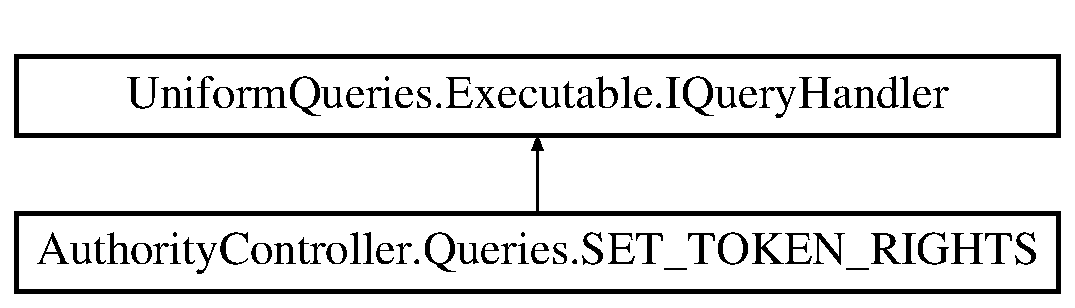
\includegraphics[height=2.000000cm]{d6/d9d/class_authority_controller_1_1_queries_1_1_s_e_t___t_o_k_e_n___r_i_g_h_t_s}
\end{center}
\end{figure}
\subsection*{Public Member Functions}
\begin{DoxyCompactItemize}
\item 
string \mbox{\hyperlink{class_authority_controller_1_1_queries_1_1_s_e_t___t_o_k_e_n___r_i_g_h_t_s_a149fb8950cf0ebbcb47b6a238c6458d2}{Description}} (string culture\+Key)
\begin{DoxyCompactList}\small\item\em Return the description relative to the lenguage code or default if not found. \end{DoxyCompactList}\item 
void \mbox{\hyperlink{class_authority_controller_1_1_queries_1_1_s_e_t___t_o_k_e_n___r_i_g_h_t_s_aebb323c8033e3a027f59c55a95695360}{Execute}} (\mbox{\hyperlink{struct_uniform_queries_1_1_query_part}{Query\+Part}}\mbox{[}$\,$\mbox{]} query\+Parts)
\begin{DoxyCompactList}\small\item\em Methods that process query. \end{DoxyCompactList}\item 
bool \mbox{\hyperlink{class_authority_controller_1_1_queries_1_1_s_e_t___t_o_k_e_n___r_i_g_h_t_s_a605feed66d357dc93ccc825068d83c96}{Is\+Target}} (\mbox{\hyperlink{struct_uniform_queries_1_1_query_part}{Query\+Part}}\mbox{[}$\,$\mbox{]} query\+Parts)
\begin{DoxyCompactList}\small\item\em Check by the entry params does it target Query Handler. \end{DoxyCompactList}\end{DoxyCompactItemize}


\subsection{Detailed Description}
Change rights list to provided token. Require admin rights. 



\subsection{Member Function Documentation}
\mbox{\Hypertarget{class_authority_controller_1_1_queries_1_1_s_e_t___t_o_k_e_n___r_i_g_h_t_s_a149fb8950cf0ebbcb47b6a238c6458d2}\label{class_authority_controller_1_1_queries_1_1_s_e_t___t_o_k_e_n___r_i_g_h_t_s_a149fb8950cf0ebbcb47b6a238c6458d2}} 
\index{Authority\+Controller\+::\+Queries\+::\+S\+E\+T\+\_\+\+T\+O\+K\+E\+N\+\_\+\+R\+I\+G\+H\+TS@{Authority\+Controller\+::\+Queries\+::\+S\+E\+T\+\_\+\+T\+O\+K\+E\+N\+\_\+\+R\+I\+G\+H\+TS}!Description@{Description}}
\index{Description@{Description}!Authority\+Controller\+::\+Queries\+::\+S\+E\+T\+\_\+\+T\+O\+K\+E\+N\+\_\+\+R\+I\+G\+H\+TS@{Authority\+Controller\+::\+Queries\+::\+S\+E\+T\+\_\+\+T\+O\+K\+E\+N\+\_\+\+R\+I\+G\+H\+TS}}
\subsubsection{\texorpdfstring{Description()}{Description()}}
{\footnotesize\ttfamily string Authority\+Controller.\+Queries.\+S\+E\+T\+\_\+\+T\+O\+K\+E\+N\+\_\+\+R\+I\+G\+H\+T\+S.\+Description (\begin{DoxyParamCaption}\item[{string}]{culture\+Key }\end{DoxyParamCaption})}



Return the description relative to the lenguage code or default if not found. 


\begin{DoxyParams}{Parameters}
{\em culture\+Key} & \\
\hline
\end{DoxyParams}
\begin{DoxyReturn}{Returns}

\end{DoxyReturn}


Implements \mbox{\hyperlink{interface_uniform_queries_1_1_executable_1_1_i_query_handler_ae0e55919571d5456af31298394d241a9}{Uniform\+Queries.\+Executable.\+I\+Query\+Handler}}.

\mbox{\Hypertarget{class_authority_controller_1_1_queries_1_1_s_e_t___t_o_k_e_n___r_i_g_h_t_s_aebb323c8033e3a027f59c55a95695360}\label{class_authority_controller_1_1_queries_1_1_s_e_t___t_o_k_e_n___r_i_g_h_t_s_aebb323c8033e3a027f59c55a95695360}} 
\index{Authority\+Controller\+::\+Queries\+::\+S\+E\+T\+\_\+\+T\+O\+K\+E\+N\+\_\+\+R\+I\+G\+H\+TS@{Authority\+Controller\+::\+Queries\+::\+S\+E\+T\+\_\+\+T\+O\+K\+E\+N\+\_\+\+R\+I\+G\+H\+TS}!Execute@{Execute}}
\index{Execute@{Execute}!Authority\+Controller\+::\+Queries\+::\+S\+E\+T\+\_\+\+T\+O\+K\+E\+N\+\_\+\+R\+I\+G\+H\+TS@{Authority\+Controller\+::\+Queries\+::\+S\+E\+T\+\_\+\+T\+O\+K\+E\+N\+\_\+\+R\+I\+G\+H\+TS}}
\subsubsection{\texorpdfstring{Execute()}{Execute()}}
{\footnotesize\ttfamily void Authority\+Controller.\+Queries.\+S\+E\+T\+\_\+\+T\+O\+K\+E\+N\+\_\+\+R\+I\+G\+H\+T\+S.\+Execute (\begin{DoxyParamCaption}\item[{\mbox{\hyperlink{struct_uniform_queries_1_1_query_part}{Query\+Part}} \mbox{[}$\,$\mbox{]}}]{query\+Parts }\end{DoxyParamCaption})}



Methods that process query. 


\begin{DoxyParams}{Parameters}
{\em query\+Parts} & \\
\hline
\end{DoxyParams}


Implements \mbox{\hyperlink{interface_uniform_queries_1_1_executable_1_1_i_query_handler_a3268d72c0388f5e3debba4d73bdfe523}{Uniform\+Queries.\+Executable.\+I\+Query\+Handler}}.

\mbox{\Hypertarget{class_authority_controller_1_1_queries_1_1_s_e_t___t_o_k_e_n___r_i_g_h_t_s_a605feed66d357dc93ccc825068d83c96}\label{class_authority_controller_1_1_queries_1_1_s_e_t___t_o_k_e_n___r_i_g_h_t_s_a605feed66d357dc93ccc825068d83c96}} 
\index{Authority\+Controller\+::\+Queries\+::\+S\+E\+T\+\_\+\+T\+O\+K\+E\+N\+\_\+\+R\+I\+G\+H\+TS@{Authority\+Controller\+::\+Queries\+::\+S\+E\+T\+\_\+\+T\+O\+K\+E\+N\+\_\+\+R\+I\+G\+H\+TS}!Is\+Target@{Is\+Target}}
\index{Is\+Target@{Is\+Target}!Authority\+Controller\+::\+Queries\+::\+S\+E\+T\+\_\+\+T\+O\+K\+E\+N\+\_\+\+R\+I\+G\+H\+TS@{Authority\+Controller\+::\+Queries\+::\+S\+E\+T\+\_\+\+T\+O\+K\+E\+N\+\_\+\+R\+I\+G\+H\+TS}}
\subsubsection{\texorpdfstring{Is\+Target()}{IsTarget()}}
{\footnotesize\ttfamily bool Authority\+Controller.\+Queries.\+S\+E\+T\+\_\+\+T\+O\+K\+E\+N\+\_\+\+R\+I\+G\+H\+T\+S.\+Is\+Target (\begin{DoxyParamCaption}\item[{\mbox{\hyperlink{struct_uniform_queries_1_1_query_part}{Query\+Part}} \mbox{[}$\,$\mbox{]}}]{query\+Parts }\end{DoxyParamCaption})}



Check by the entry params does it target Query Handler. 


\begin{DoxyParams}{Parameters}
{\em query\+Parts} & \\
\hline
\end{DoxyParams}
\begin{DoxyReturn}{Returns}

\end{DoxyReturn}


Implements \mbox{\hyperlink{interface_uniform_queries_1_1_executable_1_1_i_query_handler_a0f43184bf3e306a7cbebc39098f044ee}{Uniform\+Queries.\+Executable.\+I\+Query\+Handler}}.



The documentation for this class was generated from the following file\+:\begin{DoxyCompactItemize}
\item 
D\+:/\+Work/\+Git\+Hub/doloro-\/networking-\/framework/\+Addons/\+Authority\+Controller/\+Queries/S\+E\+T\+\_\+\+T\+O\+K\+E\+N\+\_\+\+R\+I\+G\+H\+T\+S.\+cs\end{DoxyCompactItemize}

\hypertarget{class_uniform_client_1_1_standard_1_1_simple_client}{}\section{Uniform\+Client.\+Standard.\+Simple\+Client Class Reference}
\label{class_uniform_client_1_1_standard_1_1_simple_client}\index{Uniform\+Client.\+Standard.\+Simple\+Client@{Uniform\+Client.\+Standard.\+Simple\+Client}}


Client that allow instiniate \mbox{\hyperlink{class_uniform_client_1_1_base_client}{Base\+Client}}. Not contain any additive methods.  


Inheritance diagram for Uniform\+Client.\+Standard.\+Simple\+Client\+:\begin{figure}[H]
\begin{center}
\leavevmode
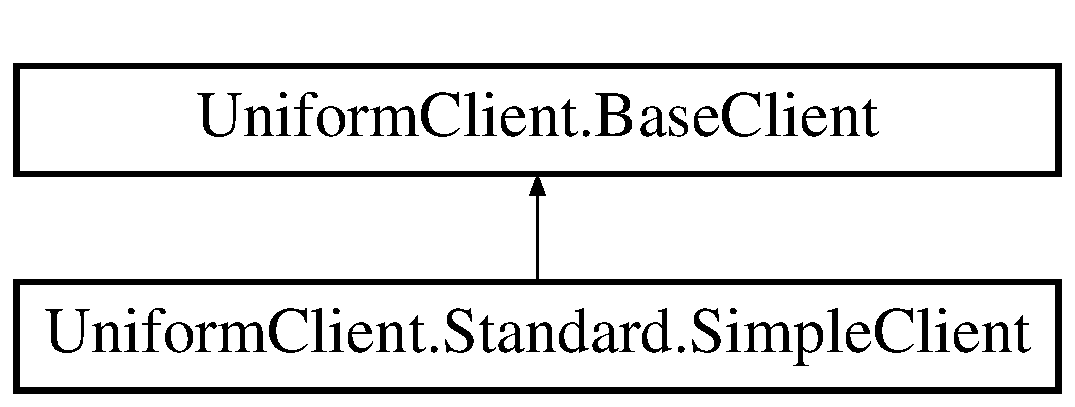
\includegraphics[height=2.000000cm]{d0/d21/class_uniform_client_1_1_standard_1_1_simple_client}
\end{center}
\end{figure}
\subsection*{Additional Inherited Members}


\subsection{Detailed Description}
Client that allow instiniate \mbox{\hyperlink{class_uniform_client_1_1_base_client}{Base\+Client}}. Not contain any additive methods. 

Case of using -\/ simple transmition line that not require complex responce. 

The documentation for this class was generated from the following file\+:\begin{DoxyCompactItemize}
\item 
D\+:/\+Work/\+Git\+Hub/doloro-\/networking-\/framework/\+Core/\+Uniform\+Client/\+Providers/\+Standard/Simple\+Client.\+cs\end{DoxyCompactItemize}

\hypertarget{class_uniform_server_1_1_standard_1_1_simple_server}{}\section{Uniform\+Server.\+Standard.\+Simple\+Server Class Reference}
\label{class_uniform_server_1_1_standard_1_1_simple_server}\index{Uniform\+Server.\+Standard.\+Simple\+Server@{Uniform\+Server.\+Standard.\+Simple\+Server}}


Server that allow instiniate \mbox{\hyperlink{class_uniform_server_1_1_base_server}{Base\+Server}}. Not contain any additive methods.  


Inheritance diagram for Uniform\+Server.\+Standard.\+Simple\+Server\+:\begin{figure}[H]
\begin{center}
\leavevmode
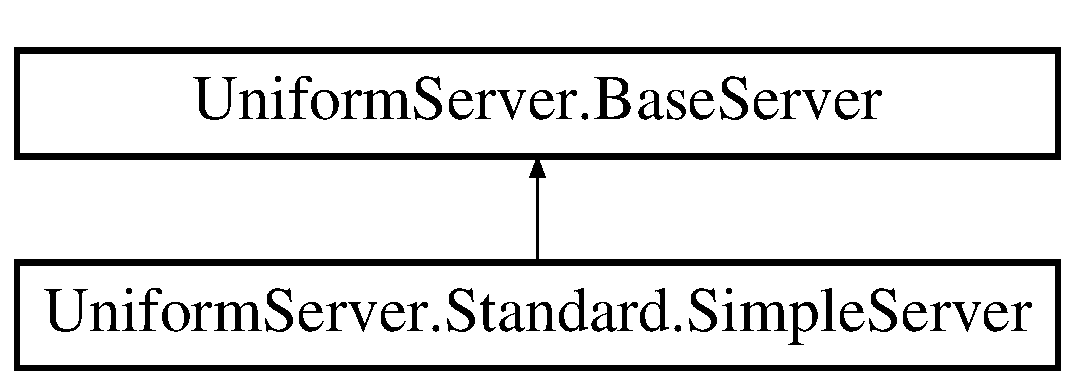
\includegraphics[height=2.000000cm]{db/daa/class_uniform_server_1_1_standard_1_1_simple_server}
\end{center}
\end{figure}
\subsection*{Additional Inherited Members}


\subsection{Detailed Description}
Server that allow instiniate \mbox{\hyperlink{class_uniform_server_1_1_base_server}{Base\+Server}}. Not contain any additive methods. 

Case of using -\/ simple operations like registing of server for answer. 

The documentation for this class was generated from the following file\+:\begin{DoxyCompactItemize}
\item 
D\+:/\+Work/\+Git\+Hub/doloro-\/networking-\/framework/\+Core/\+D\+N\+F\+Core/\+Uniform\+Server/\+Providers/\+Standard/Simple\+Server.\+cs\end{DoxyCompactItemize}

\hypertarget{class_authority_controller_1_1_data_1_1_temporal_1_1_token_info}{}\section{Authority\+Controller.\+Data.\+Temporal.\+Token\+Info Class Reference}
\label{class_authority_controller_1_1_data_1_1_temporal_1_1_token_info}\index{Authority\+Controller.\+Data.\+Temporal.\+Token\+Info@{Authority\+Controller.\+Data.\+Temporal.\+Token\+Info}}


Container that contain data about token.  


\subsection*{Public Attributes}
\begin{DoxyCompactItemize}
\item 
string \mbox{\hyperlink{class_authority_controller_1_1_data_1_1_temporal_1_1_token_info_a9856f3e8590d95c39e2c2802b133fef4}{token}}
\begin{DoxyCompactList}\small\item\em Token string. \end{DoxyCompactList}\item 
string \mbox{\hyperlink{class_authority_controller_1_1_data_1_1_temporal_1_1_token_info_a4aa8e73482b707625aa8d1a2a1d580db}{operation\+System}}
\begin{DoxyCompactList}\small\item\em Operation system that request this token. Using for machine stamp. \end{DoxyCompactList}\item 
string \mbox{\hyperlink{class_authority_controller_1_1_data_1_1_temporal_1_1_token_info_a8b2962c8de8ad0d43204fdae97d1393f}{machine\+Mac}}
\begin{DoxyCompactList}\small\item\em Mac adress of machine that request access. Using for machine stamp. \end{DoxyCompactList}\item 
uint \mbox{\hyperlink{class_authority_controller_1_1_data_1_1_temporal_1_1_token_info_ae27c8979079353983244db00920b1501}{user\+Id}}
\begin{DoxyCompactList}\small\item\em Id of user that recive this token. \end{DoxyCompactList}\item 
long \mbox{\hyperlink{class_authority_controller_1_1_data_1_1_temporal_1_1_token_info_acce187b055ae59b52d704b7dfcd4b74d}{allocation\+Time}}
\begin{DoxyCompactList}\small\item\em Time when token was allocated in system. \end{DoxyCompactList}\item 
string \mbox{[}$\,$\mbox{]} \mbox{\hyperlink{class_authority_controller_1_1_data_1_1_temporal_1_1_token_info_aa1919ec575894ea2ff957f87d3428dc7}{rights}}
\begin{DoxyCompactList}\small\item\em Array that contain rights provided to this token. \end{DoxyCompactList}\end{DoxyCompactItemize}
\subsection*{Properties}
\begin{DoxyCompactItemize}
\item 
static \mbox{\hyperlink{class_authority_controller_1_1_data_1_1_temporal_1_1_token_info}{Token\+Info}} \mbox{\hyperlink{class_authority_controller_1_1_data_1_1_temporal_1_1_token_info_acab070b9dcca472286bc953501989df0}{Anonymous}}\hspace{0.3cm}{\ttfamily  \mbox{[}get\mbox{]}}
\begin{DoxyCompactList}\small\item\em Return empty info. \end{DoxyCompactList}\end{DoxyCompactItemize}


\subsection{Detailed Description}
Container that contain data about token. 



\subsection{Member Data Documentation}
\mbox{\Hypertarget{class_authority_controller_1_1_data_1_1_temporal_1_1_token_info_acce187b055ae59b52d704b7dfcd4b74d}\label{class_authority_controller_1_1_data_1_1_temporal_1_1_token_info_acce187b055ae59b52d704b7dfcd4b74d}} 
\index{Authority\+Controller\+::\+Data\+::\+Temporal\+::\+Token\+Info@{Authority\+Controller\+::\+Data\+::\+Temporal\+::\+Token\+Info}!allocation\+Time@{allocation\+Time}}
\index{allocation\+Time@{allocation\+Time}!Authority\+Controller\+::\+Data\+::\+Temporal\+::\+Token\+Info@{Authority\+Controller\+::\+Data\+::\+Temporal\+::\+Token\+Info}}
\subsubsection{\texorpdfstring{allocation\+Time}{allocationTime}}
{\footnotesize\ttfamily long Authority\+Controller.\+Data.\+Temporal.\+Token\+Info.\+allocation\+Time}



Time when token was allocated in system. 

\mbox{\Hypertarget{class_authority_controller_1_1_data_1_1_temporal_1_1_token_info_a8b2962c8de8ad0d43204fdae97d1393f}\label{class_authority_controller_1_1_data_1_1_temporal_1_1_token_info_a8b2962c8de8ad0d43204fdae97d1393f}} 
\index{Authority\+Controller\+::\+Data\+::\+Temporal\+::\+Token\+Info@{Authority\+Controller\+::\+Data\+::\+Temporal\+::\+Token\+Info}!machine\+Mac@{machine\+Mac}}
\index{machine\+Mac@{machine\+Mac}!Authority\+Controller\+::\+Data\+::\+Temporal\+::\+Token\+Info@{Authority\+Controller\+::\+Data\+::\+Temporal\+::\+Token\+Info}}
\subsubsection{\texorpdfstring{machine\+Mac}{machineMac}}
{\footnotesize\ttfamily string Authority\+Controller.\+Data.\+Temporal.\+Token\+Info.\+machine\+Mac}



Mac adress of machine that request access. Using for machine stamp. 

\mbox{\Hypertarget{class_authority_controller_1_1_data_1_1_temporal_1_1_token_info_a4aa8e73482b707625aa8d1a2a1d580db}\label{class_authority_controller_1_1_data_1_1_temporal_1_1_token_info_a4aa8e73482b707625aa8d1a2a1d580db}} 
\index{Authority\+Controller\+::\+Data\+::\+Temporal\+::\+Token\+Info@{Authority\+Controller\+::\+Data\+::\+Temporal\+::\+Token\+Info}!operation\+System@{operation\+System}}
\index{operation\+System@{operation\+System}!Authority\+Controller\+::\+Data\+::\+Temporal\+::\+Token\+Info@{Authority\+Controller\+::\+Data\+::\+Temporal\+::\+Token\+Info}}
\subsubsection{\texorpdfstring{operation\+System}{operationSystem}}
{\footnotesize\ttfamily string Authority\+Controller.\+Data.\+Temporal.\+Token\+Info.\+operation\+System}



Operation system that request this token. Using for machine stamp. 

\mbox{\Hypertarget{class_authority_controller_1_1_data_1_1_temporal_1_1_token_info_aa1919ec575894ea2ff957f87d3428dc7}\label{class_authority_controller_1_1_data_1_1_temporal_1_1_token_info_aa1919ec575894ea2ff957f87d3428dc7}} 
\index{Authority\+Controller\+::\+Data\+::\+Temporal\+::\+Token\+Info@{Authority\+Controller\+::\+Data\+::\+Temporal\+::\+Token\+Info}!rights@{rights}}
\index{rights@{rights}!Authority\+Controller\+::\+Data\+::\+Temporal\+::\+Token\+Info@{Authority\+Controller\+::\+Data\+::\+Temporal\+::\+Token\+Info}}
\subsubsection{\texorpdfstring{rights}{rights}}
{\footnotesize\ttfamily string \mbox{[}$\,$\mbox{]} Authority\+Controller.\+Data.\+Temporal.\+Token\+Info.\+rights}



Array that contain rights provided to this token. 

\mbox{\Hypertarget{class_authority_controller_1_1_data_1_1_temporal_1_1_token_info_a9856f3e8590d95c39e2c2802b133fef4}\label{class_authority_controller_1_1_data_1_1_temporal_1_1_token_info_a9856f3e8590d95c39e2c2802b133fef4}} 
\index{Authority\+Controller\+::\+Data\+::\+Temporal\+::\+Token\+Info@{Authority\+Controller\+::\+Data\+::\+Temporal\+::\+Token\+Info}!token@{token}}
\index{token@{token}!Authority\+Controller\+::\+Data\+::\+Temporal\+::\+Token\+Info@{Authority\+Controller\+::\+Data\+::\+Temporal\+::\+Token\+Info}}
\subsubsection{\texorpdfstring{token}{token}}
{\footnotesize\ttfamily string Authority\+Controller.\+Data.\+Temporal.\+Token\+Info.\+token}



Token string. 

\mbox{\Hypertarget{class_authority_controller_1_1_data_1_1_temporal_1_1_token_info_ae27c8979079353983244db00920b1501}\label{class_authority_controller_1_1_data_1_1_temporal_1_1_token_info_ae27c8979079353983244db00920b1501}} 
\index{Authority\+Controller\+::\+Data\+::\+Temporal\+::\+Token\+Info@{Authority\+Controller\+::\+Data\+::\+Temporal\+::\+Token\+Info}!user\+Id@{user\+Id}}
\index{user\+Id@{user\+Id}!Authority\+Controller\+::\+Data\+::\+Temporal\+::\+Token\+Info@{Authority\+Controller\+::\+Data\+::\+Temporal\+::\+Token\+Info}}
\subsubsection{\texorpdfstring{user\+Id}{userId}}
{\footnotesize\ttfamily uint Authority\+Controller.\+Data.\+Temporal.\+Token\+Info.\+user\+Id}



Id of user that recive this token. 



\subsection{Property Documentation}
\mbox{\Hypertarget{class_authority_controller_1_1_data_1_1_temporal_1_1_token_info_acab070b9dcca472286bc953501989df0}\label{class_authority_controller_1_1_data_1_1_temporal_1_1_token_info_acab070b9dcca472286bc953501989df0}} 
\index{Authority\+Controller\+::\+Data\+::\+Temporal\+::\+Token\+Info@{Authority\+Controller\+::\+Data\+::\+Temporal\+::\+Token\+Info}!Anonymous@{Anonymous}}
\index{Anonymous@{Anonymous}!Authority\+Controller\+::\+Data\+::\+Temporal\+::\+Token\+Info@{Authority\+Controller\+::\+Data\+::\+Temporal\+::\+Token\+Info}}
\subsubsection{\texorpdfstring{Anonymous}{Anonymous}}
{\footnotesize\ttfamily \mbox{\hyperlink{class_authority_controller_1_1_data_1_1_temporal_1_1_token_info}{Token\+Info}} Authority\+Controller.\+Data.\+Temporal.\+Token\+Info.\+Anonymous\hspace{0.3cm}{\ttfamily [static]}, {\ttfamily [get]}}



Return empty info. 



The documentation for this class was generated from the following file\+:\begin{DoxyCompactItemize}
\item 
D\+:/\+Work/\+Git\+Hub/doloro-\/networking-\/framework/\+Addons/\+Authority\+Controller/\+Data/\+Temporal/Token\+Info.\+cs\end{DoxyCompactItemize}

\hypertarget{class_uniform_queries_1_1_tokens}{}\section{Uniform\+Queries.\+Tokens Class Reference}
\label{class_uniform_queries_1_1_tokens}\index{Uniform\+Queries.\+Tokens@{Uniform\+Queries.\+Tokens}}
\subsection*{Static Public Member Functions}
\begin{DoxyCompactItemize}
\item 
static bool \mbox{\hyperlink{class_uniform_queries_1_1_tokens_a33a0ad42dfa560c4cfaac590a7924bd8}{Is\+Expired}} (string token, Date\+Time expiry\+Time)
\begin{DoxyCompactList}\small\item\em Check if token expired based on encoded token data. Use it on Queries Server to avoid additive time spending on data servers and unnecessary connections. \end{DoxyCompactList}\end{DoxyCompactItemize}
\subsection*{Properties}
\begin{DoxyCompactItemize}
\item 
static string \mbox{\hyperlink{class_uniform_queries_1_1_tokens_af591930ab4fa60ebdf27724f84ac7a91}{Unused\+Token}}\hspace{0.3cm}{\ttfamily  \mbox{[}get\mbox{]}}
\begin{DoxyCompactList}\small\item\em Return free token. \end{DoxyCompactList}\end{DoxyCompactItemize}


\subsection{Member Function Documentation}
\mbox{\Hypertarget{class_uniform_queries_1_1_tokens_a33a0ad42dfa560c4cfaac590a7924bd8}\label{class_uniform_queries_1_1_tokens_a33a0ad42dfa560c4cfaac590a7924bd8}} 
\index{Uniform\+Queries\+::\+Tokens@{Uniform\+Queries\+::\+Tokens}!Is\+Expired@{Is\+Expired}}
\index{Is\+Expired@{Is\+Expired}!Uniform\+Queries\+::\+Tokens@{Uniform\+Queries\+::\+Tokens}}
\subsubsection{\texorpdfstring{Is\+Expired()}{IsExpired()}}
{\footnotesize\ttfamily static bool Uniform\+Queries.\+Tokens.\+Is\+Expired (\begin{DoxyParamCaption}\item[{string}]{token,  }\item[{Date\+Time}]{expiry\+Time }\end{DoxyParamCaption})\hspace{0.3cm}{\ttfamily [static]}}



Check if token expired based on encoded token data. Use it on Queries Server to avoid additive time spending on data servers and unnecessary connections. 

If token have hacked allocate date this just will lead to passing of this check. Server wouldn\textquotesingle{}t has has token so sequrity will not be passed. Also server will control expire time by him self. 


\begin{DoxyParams}{Parameters}
{\em token} & Token in string format.\\
\hline
{\em expiry\+Time} & Time when token would expired.\\
\hline
\end{DoxyParams}
\begin{DoxyReturn}{Returns}

\end{DoxyReturn}


\subsection{Property Documentation}
\mbox{\Hypertarget{class_uniform_queries_1_1_tokens_af591930ab4fa60ebdf27724f84ac7a91}\label{class_uniform_queries_1_1_tokens_af591930ab4fa60ebdf27724f84ac7a91}} 
\index{Uniform\+Queries\+::\+Tokens@{Uniform\+Queries\+::\+Tokens}!Unused\+Token@{Unused\+Token}}
\index{Unused\+Token@{Unused\+Token}!Uniform\+Queries\+::\+Tokens@{Uniform\+Queries\+::\+Tokens}}
\subsubsection{\texorpdfstring{Unused\+Token}{UnusedToken}}
{\footnotesize\ttfamily string Uniform\+Queries.\+Tokens.\+Unused\+Token\hspace{0.3cm}{\ttfamily [static]}, {\ttfamily [get]}}



Return free token. 



The documentation for this class was generated from the following file\+:\begin{DoxyCompactItemize}
\item 
D\+:/\+Work/\+Git\+Hub/doloro-\/networking-\/framework/\+Core/\+Uniform\+Queries/Tokens.\+cs\end{DoxyCompactItemize}

\hypertarget{class_authority_controller_1_1_a_p_i_1_1_tokens}{}\section{Authority\+Controller.\+A\+P\+I.\+Tokens Class Reference}
\label{class_authority_controller_1_1_a_p_i_1_1_tokens}\index{Authority\+Controller.\+A\+P\+I.\+Tokens@{Authority\+Controller.\+A\+P\+I.\+Tokens}}
\subsection*{Static Public Member Functions}
\begin{DoxyCompactItemize}
\item 
static bool \mbox{\hyperlink{class_authority_controller_1_1_a_p_i_1_1_tokens_acbc5a5df26ae29633d4424873676ece3}{Is\+Expired}} (string token)
\begin{DoxyCompactList}\small\item\em Check if token expired based on encoded token data. Use it on \mbox{\hyperlink{namespace_authority_controller_1_1_queries}{Queries}} Server to avoid additive time spending on data servers and unnecessary connections. \end{DoxyCompactList}\item 
static bool \mbox{\hyperlink{class_authority_controller_1_1_a_p_i_1_1_tokens_a3077a786044bdd530ad50dbd615f8beb}{Is\+Has\+Enough\+Rigths}} (string token, out string\mbox{[}$\,$\mbox{]} requester\+Rights, out string error, params string\mbox{[}$\,$\mbox{]} required\+Rights)
\begin{DoxyCompactList}\small\item\em Check does this token has all requested rights. If token is not registred on this server then will throw Unauthorized\+Access\+Exception. \end{DoxyCompactList}\item 
static bool \mbox{\hyperlink{class_authority_controller_1_1_a_p_i_1_1_tokens_ab1d580a971a86c8e5b3c7c189aa65381}{Is\+Has\+Enough\+Rigths}} (string token, out string\mbox{[}$\,$\mbox{]} requester\+Rights, params string\mbox{[}$\,$\mbox{]} required\+Rights)
\begin{DoxyCompactList}\small\item\em Check does this token has all requested rights. If token is not registred on this server then will throw Unauthorized\+Access\+Exception. \end{DoxyCompactList}\item 
static string \mbox{\hyperlink{class_authority_controller_1_1_a_p_i_1_1_tokens_a0ba1c2d69ffbc73d78b7b16735f7fb5a}{Authorize\+New\+Guest\+Token}} ()
\begin{DoxyCompactList}\small\item\em Authorizing new token with guest\textquotesingle{}s rights, and return information in query format. \end{DoxyCompactList}\end{DoxyCompactItemize}
\subsection*{Properties}
\begin{DoxyCompactItemize}
\item 
static string \mbox{\hyperlink{class_authority_controller_1_1_a_p_i_1_1_tokens_a43a1d7e3b2fa6ed94a20dc7b1e36b27a}{Unused\+Token}}\hspace{0.3cm}{\ttfamily  \mbox{[}get\mbox{]}}
\begin{DoxyCompactList}\small\item\em Return free token. \end{DoxyCompactList}\end{DoxyCompactItemize}


\subsection{Member Function Documentation}
\mbox{\Hypertarget{class_authority_controller_1_1_a_p_i_1_1_tokens_a0ba1c2d69ffbc73d78b7b16735f7fb5a}\label{class_authority_controller_1_1_a_p_i_1_1_tokens_a0ba1c2d69ffbc73d78b7b16735f7fb5a}} 
\index{Authority\+Controller\+::\+A\+P\+I\+::\+Tokens@{Authority\+Controller\+::\+A\+P\+I\+::\+Tokens}!Authorize\+New\+Guest\+Token@{Authorize\+New\+Guest\+Token}}
\index{Authorize\+New\+Guest\+Token@{Authorize\+New\+Guest\+Token}!Authority\+Controller\+::\+A\+P\+I\+::\+Tokens@{Authority\+Controller\+::\+A\+P\+I\+::\+Tokens}}
\subsubsection{\texorpdfstring{Authorize\+New\+Guest\+Token()}{AuthorizeNewGuestToken()}}
{\footnotesize\ttfamily static string Authority\+Controller.\+A\+P\+I.\+Tokens.\+Authorize\+New\+Guest\+Token (\begin{DoxyParamCaption}{ }\end{DoxyParamCaption})\hspace{0.3cm}{\ttfamily [static]}}



Authorizing new token with guest\textquotesingle{}s rights, and return information in query format. 

\begin{DoxyReturn}{Returns}
Token that can be used by client in queries.
\end{DoxyReturn}
\mbox{\Hypertarget{class_authority_controller_1_1_a_p_i_1_1_tokens_acbc5a5df26ae29633d4424873676ece3}\label{class_authority_controller_1_1_a_p_i_1_1_tokens_acbc5a5df26ae29633d4424873676ece3}} 
\index{Authority\+Controller\+::\+A\+P\+I\+::\+Tokens@{Authority\+Controller\+::\+A\+P\+I\+::\+Tokens}!Is\+Expired@{Is\+Expired}}
\index{Is\+Expired@{Is\+Expired}!Authority\+Controller\+::\+A\+P\+I\+::\+Tokens@{Authority\+Controller\+::\+A\+P\+I\+::\+Tokens}}
\subsubsection{\texorpdfstring{Is\+Expired()}{IsExpired()}}
{\footnotesize\ttfamily static bool Authority\+Controller.\+A\+P\+I.\+Tokens.\+Is\+Expired (\begin{DoxyParamCaption}\item[{string}]{token }\end{DoxyParamCaption})\hspace{0.3cm}{\ttfamily [static]}}



Check if token expired based on encoded token data. Use it on \mbox{\hyperlink{namespace_authority_controller_1_1_queries}{Queries}} Server to avoid additive time spending on data servers and unnecessary connections. 

If token have hacked allocate date this just will lead to passing of this check. Server wouldn\textquotesingle{}t has has token so sequrity will not be passed. Also server will control expire time by him self. 


\begin{DoxyParams}{Parameters}
{\em token} & \\
\hline
\end{DoxyParams}
\begin{DoxyReturn}{Returns}

\end{DoxyReturn}
\mbox{\Hypertarget{class_authority_controller_1_1_a_p_i_1_1_tokens_a3077a786044bdd530ad50dbd615f8beb}\label{class_authority_controller_1_1_a_p_i_1_1_tokens_a3077a786044bdd530ad50dbd615f8beb}} 
\index{Authority\+Controller\+::\+A\+P\+I\+::\+Tokens@{Authority\+Controller\+::\+A\+P\+I\+::\+Tokens}!Is\+Has\+Enough\+Rigths@{Is\+Has\+Enough\+Rigths}}
\index{Is\+Has\+Enough\+Rigths@{Is\+Has\+Enough\+Rigths}!Authority\+Controller\+::\+A\+P\+I\+::\+Tokens@{Authority\+Controller\+::\+A\+P\+I\+::\+Tokens}}
\subsubsection{\texorpdfstring{Is\+Has\+Enough\+Rigths()}{IsHasEnoughRigths()}\hspace{0.1cm}{\footnotesize\ttfamily [1/2]}}
{\footnotesize\ttfamily static bool Authority\+Controller.\+A\+P\+I.\+Tokens.\+Is\+Has\+Enough\+Rigths (\begin{DoxyParamCaption}\item[{string}]{token,  }\item[{out string \mbox{[}$\,$\mbox{]}}]{requester\+Rights,  }\item[{out string}]{error,  }\item[{params string \mbox{[}$\,$\mbox{]}}]{required\+Rights }\end{DoxyParamCaption})\hspace{0.3cm}{\ttfamily [static]}}



Check does this token has all requested rights. If token is not registred on this server then will throw Unauthorized\+Access\+Exception. 


\begin{DoxyParams}{Parameters}
{\em token} & Unitque token of the user.\\
\hline
{\em error} & Error that describe a reasone of fail. Could be send backward to client.\\
\hline
{\em requester\+Rights} & Rights detected to that token.\\
\hline
{\em required\+Rights} & Array that contain the rights that need to by existed.\\
\hline
\end{DoxyParams}
\begin{DoxyReturn}{Returns}

\end{DoxyReturn}
\mbox{\Hypertarget{class_authority_controller_1_1_a_p_i_1_1_tokens_ab1d580a971a86c8e5b3c7c189aa65381}\label{class_authority_controller_1_1_a_p_i_1_1_tokens_ab1d580a971a86c8e5b3c7c189aa65381}} 
\index{Authority\+Controller\+::\+A\+P\+I\+::\+Tokens@{Authority\+Controller\+::\+A\+P\+I\+::\+Tokens}!Is\+Has\+Enough\+Rigths@{Is\+Has\+Enough\+Rigths}}
\index{Is\+Has\+Enough\+Rigths@{Is\+Has\+Enough\+Rigths}!Authority\+Controller\+::\+A\+P\+I\+::\+Tokens@{Authority\+Controller\+::\+A\+P\+I\+::\+Tokens}}
\subsubsection{\texorpdfstring{Is\+Has\+Enough\+Rigths()}{IsHasEnoughRigths()}\hspace{0.1cm}{\footnotesize\ttfamily [2/2]}}
{\footnotesize\ttfamily static bool Authority\+Controller.\+A\+P\+I.\+Tokens.\+Is\+Has\+Enough\+Rigths (\begin{DoxyParamCaption}\item[{string}]{token,  }\item[{out string \mbox{[}$\,$\mbox{]}}]{requester\+Rights,  }\item[{params string \mbox{[}$\,$\mbox{]}}]{required\+Rights }\end{DoxyParamCaption})\hspace{0.3cm}{\ttfamily [static]}}



Check does this token has all requested rights. If token is not registred on this server then will throw Unauthorized\+Access\+Exception. 


\begin{DoxyParams}{Parameters}
{\em token} & \\
\hline
{\em required\+Rights} & \\
\hline
{\em requester\+Rights} & Rights detected to that token.\\
\hline
\end{DoxyParams}
\begin{DoxyReturn}{Returns}

\end{DoxyReturn}


\subsection{Property Documentation}
\mbox{\Hypertarget{class_authority_controller_1_1_a_p_i_1_1_tokens_a43a1d7e3b2fa6ed94a20dc7b1e36b27a}\label{class_authority_controller_1_1_a_p_i_1_1_tokens_a43a1d7e3b2fa6ed94a20dc7b1e36b27a}} 
\index{Authority\+Controller\+::\+A\+P\+I\+::\+Tokens@{Authority\+Controller\+::\+A\+P\+I\+::\+Tokens}!Unused\+Token@{Unused\+Token}}
\index{Unused\+Token@{Unused\+Token}!Authority\+Controller\+::\+A\+P\+I\+::\+Tokens@{Authority\+Controller\+::\+A\+P\+I\+::\+Tokens}}
\subsubsection{\texorpdfstring{Unused\+Token}{UnusedToken}}
{\footnotesize\ttfamily string Authority\+Controller.\+A\+P\+I.\+Tokens.\+Unused\+Token\hspace{0.3cm}{\ttfamily [static]}, {\ttfamily [get]}}



Return free token. 



The documentation for this class was generated from the following file\+:\begin{DoxyCompactItemize}
\item 
D\+:/\+Work/\+Git\+Hub/doloro-\/networking-\/framework/\+Addons/\+Authority\+Controller/\+A\+P\+I/Tokens.\+cs\end{DoxyCompactItemize}

\hypertarget{class_pipes_provider_1_1_client_1_1_transmission_line}{}\section{Pipes\+Provider.\+Client.\+Transmission\+Line Class Reference}
\label{class_pipes_provider_1_1_client_1_1_transmission_line}\index{Pipes\+Provider.\+Client.\+Transmission\+Line@{Pipes\+Provider.\+Client.\+Transmission\+Line}}


Class that provide information about line between client and server. Provide A\+PI to easy control. Provide automatic services.  


\subsection*{Public Types}
\begin{DoxyCompactItemize}
\item 
\mbox{\Hypertarget{class_pipes_provider_1_1_client_1_1_transmission_line_adf7f55a4fb34b6503ef72d8b562b2ff5}\label{class_pipes_provider_1_1_client_1_1_transmission_line_adf7f55a4fb34b6503ef72d8b562b2ff5}} 
enum {\bfseries Transmission\+Direction} \{ {\bfseries In}, 
{\bfseries Out}
 \}
\end{DoxyCompactItemize}
\subsection*{Public Member Functions}
\begin{DoxyCompactItemize}
\item 
\mbox{\hyperlink{class_pipes_provider_1_1_client_1_1_transmission_line_a8fe76e563974e7380fe2f717e48d694e}{Transmission\+Line}} (string server\+Name, string server\+Pipe\+Name, System.\+Action$<$ \mbox{\hyperlink{class_pipes_provider_1_1_client_1_1_transmission_line}{Transmission\+Line}} $>$ \mbox{\hyperlink{class_pipes_provider_1_1_client_1_1_transmission_line_a86f49118056ad8cb6fe383abb2a350e8}{query\+Processor}}, ref Safe\+Access\+Token\+Handle token)
\begin{DoxyCompactList}\small\item\em Create new instance of Line\+Processor taht can be registread in static services. Contain information about transmission between client and server. \end{DoxyCompactList}\item 
\mbox{\hyperlink{class_pipes_provider_1_1_client_1_1_transmission_line_aa75228335f18b62a772bd43db9587e42}{Transmission\+Line}} (ref \mbox{\hyperlink{class_pipes_provider_1_1_networking_1_1_routing_1_1_instruction}{Instruction}} instruction, System.\+Action$<$ \mbox{\hyperlink{class_pipes_provider_1_1_client_1_1_transmission_line}{Transmission\+Line}} $>$ \mbox{\hyperlink{class_pipes_provider_1_1_client_1_1_transmission_line_a86f49118056ad8cb6fe383abb2a350e8}{query\+Processor}})
\begin{DoxyCompactList}\small\item\em Create instance using routing instruction. \end{DoxyCompactList}\item 
\mbox{\hyperlink{class_pipes_provider_1_1_client_1_1_transmission_line}{Transmission\+Line}} \mbox{\hyperlink{class_pipes_provider_1_1_client_1_1_transmission_line_ac7a9bbb2d71ae7080788b28449b216fc}{Enqueue\+Query}} (string query)
\begin{DoxyCompactList}\small\item\em Enqueue query to order. Query will be posted to server as soon as will possible. \end{DoxyCompactList}\item 
\mbox{\hyperlink{class_pipes_provider_1_1_client_1_1_transmission_line}{Transmission\+Line}} \mbox{\hyperlink{class_pipes_provider_1_1_client_1_1_transmission_line_a0adfc0db736cc9315a6e1c0ea04c42e6}{Enqueue\+Query}} (\mbox{\hyperlink{struct_pipes_provider_1_1_client_1_1_query_container}{Query\+Container}} query)
\begin{DoxyCompactList}\small\item\em Enqueue query to order. Query will be posted to server as soon as will possible. \end{DoxyCompactList}\item 
bool \mbox{\hyperlink{class_pipes_provider_1_1_client_1_1_transmission_line_a48c6395608b4d32a7d852c2fd6d911e2}{Try\+Deque\+Query}} (out \mbox{\hyperlink{struct_pipes_provider_1_1_client_1_1_query_container}{Query\+Container}} query)
\begin{DoxyCompactList}\small\item\em Try to get a new query in turn. \end{DoxyCompactList}\item 
void \mbox{\hyperlink{class_pipes_provider_1_1_client_1_1_transmission_line_a5d921e9d7b0dfb366d79c6397bec9179}{Close}} ()
\begin{DoxyCompactList}\small\item\em Mark line as closed. Thread will be terminated on the next client tick. \end{DoxyCompactList}\item 
void \mbox{\hyperlink{class_pipes_provider_1_1_client_1_1_transmission_line_ae2d45dea3d22625d81634a6eea3cd356}{Drop\+Meta}} ()
\begin{DoxyCompactList}\small\item\em Drop meta data relative only per one session. \end{DoxyCompactList}\item 
bool \mbox{\hyperlink{class_pipes_provider_1_1_client_1_1_transmission_line_a75c4a1aa309fbc60cccbe258a85a91b3}{Try\+Logon\+As}} (\mbox{\hyperlink{struct_pipes_provider_1_1_security_1_1_logon_config}{Security.\+Logon\+Config}} logon\+Meta)
\begin{DoxyCompactList}\small\item\em Trying to logon using provided information. In case failed -\/ close line. \end{DoxyCompactList}\item 
\mbox{\hyperlink{class_pipes_provider_1_1_client_1_1_transmission_line}{Transmission\+Line}} \mbox{\hyperlink{class_pipes_provider_1_1_client_1_1_transmission_line_a2741ab56f9eecbe0bcbd018232321205}{Set\+Instruction\+As\+Key}} (ref \mbox{\hyperlink{class_pipes_provider_1_1_networking_1_1_routing_1_1_instruction}{Instruction}} instruction)
\begin{DoxyCompactList}\small\item\em Set routing instruction to line. Provide access to auto messages encryption with control of keys expiring. \end{DoxyCompactList}\end{DoxyCompactItemize}
\subsection*{Static Public Member Functions}
\begin{DoxyCompactItemize}
\item 
static \mbox{\hyperlink{class_pipes_provider_1_1_client_1_1_transmission_line}{Transmission\+Line}} \mbox{\hyperlink{class_pipes_provider_1_1_client_1_1_transmission_line_ada994593c98fe9aa24abb0a3ab55e6e2}{operator++}} (\mbox{\hyperlink{class_pipes_provider_1_1_client_1_1_transmission_line}{Transmission\+Line}} line)
\begin{DoxyCompactList}\small\item\em Incremet of attempts count. \end{DoxyCompactList}\item 
static void \mbox{\hyperlink{class_pipes_provider_1_1_client_1_1_transmission_line_aebf1f90d880307f803bdeb6e0020a95f}{Thread\+Loop}} (object line\+Processor)
\begin{DoxyCompactList}\small\item\em Method that can be started as thread. Will start client loop. \end{DoxyCompactList}\item 
static string \mbox{\hyperlink{class_pipes_provider_1_1_client_1_1_transmission_line_a334cde78dd1b3cc6c3cb2a6bb7419a1d}{Generate\+G\+U\+ID}} (string server\+Name, string pipe\+Name)
\begin{DoxyCompactList}\small\item\em Generate G\+U\+ID of this transmission line relative to pipe params. \end{DoxyCompactList}\end{DoxyCompactItemize}
\subsection*{Public Attributes}
\begin{DoxyCompactItemize}
\item 
Safe\+Access\+Token\+Handle \mbox{\hyperlink{class_pipes_provider_1_1_client_1_1_transmission_line_adad9bc543ae01a23e792f46bf3b3092f}{access\+Token}}
\begin{DoxyCompactList}\small\item\em Token that will used to autorizing on the server. \end{DoxyCompactList}\item 
Named\+Pipe\+Client\+Stream \mbox{\hyperlink{class_pipes_provider_1_1_client_1_1_transmission_line_a617db258fff1a28c80ff7d6241e8372e}{pipe\+Client}}
\begin{DoxyCompactList}\small\item\em Reference to the current oppened pipe. \end{DoxyCompactList}\item 
System.\+Action$<$ \mbox{\hyperlink{class_pipes_provider_1_1_client_1_1_transmission_line}{Transmission\+Line}} $>$ \mbox{\hyperlink{class_pipes_provider_1_1_client_1_1_transmission_line_a86f49118056ad8cb6fe383abb2a350e8}{query\+Processor}}
\begin{DoxyCompactList}\small\item\em This delegate will be callback when connection wfor qury will be established. \end{DoxyCompactList}\end{DoxyCompactItemize}
\subsection*{Protected Attributes}
\begin{DoxyCompactItemize}
\item 
\mbox{\hyperlink{struct_pipes_provider_1_1_client_1_1_query_container}{Query\+Container}} \mbox{\hyperlink{class_pipes_provider_1_1_client_1_1_transmission_line_ac58ee721ec6876da25190b15d52530a3}{last\+Query}} = \mbox{\hyperlink{struct_pipes_provider_1_1_client_1_1_query_container_a0e1f91d0a990824b56170c3da5e5919c}{Query\+Container.\+Empty}}
\begin{DoxyCompactList}\small\item\em Field that contain last dequeued query. \end{DoxyCompactList}\item 
Queue$<$ \mbox{\hyperlink{struct_pipes_provider_1_1_client_1_1_query_container}{Query\+Container}} $>$ \mbox{\hyperlink{class_pipes_provider_1_1_client_1_1_transmission_line_af110134a03e1e046911970fff4774600}{queries}} = new Queue$<$\mbox{\hyperlink{struct_pipes_provider_1_1_client_1_1_query_container}{Query\+Container}}$>$()
\begin{DoxyCompactList}\small\item\em List of queries that will wait its order to access transmission via this line. \end{DoxyCompactList}\end{DoxyCompactItemize}
\subsection*{Properties}
\begin{DoxyCompactItemize}
\item 
string \mbox{\hyperlink{class_pipes_provider_1_1_client_1_1_transmission_line_a6959acebfbb30be2aa0149779bc6822c}{G\+U\+ID}}\hspace{0.3cm}{\ttfamily  \mbox{[}get\mbox{]}}
\begin{DoxyCompactList}\small\item\em Unique G\+U\+ID for this pipe. \end{DoxyCompactList}\item 
string \mbox{\hyperlink{class_pipes_provider_1_1_client_1_1_transmission_line_aa7e8a85952e05718b1a0ff96b9874766}{Server\+Pipe\+Name}}\hspace{0.3cm}{\ttfamily  \mbox{[}get, protected set\mbox{]}}
\begin{DoxyCompactList}\small\item\em Name of server pipe that will be using for transmission via current processor. \end{DoxyCompactList}\item 
string \mbox{\hyperlink{class_pipes_provider_1_1_client_1_1_transmission_line_a3dc08ad974186de6b0439b052ea0d72a}{Server\+Name}}\hspace{0.3cm}{\ttfamily  \mbox{[}get, protected set\mbox{]}}
\begin{DoxyCompactList}\small\item\em Name of server pipe that will be using for transmission via current processor. \end{DoxyCompactList}\item 
bool \mbox{\hyperlink{class_pipes_provider_1_1_client_1_1_transmission_line_a902851edce28b2ab7a7b9fc648a984d5}{Closed}}\hspace{0.3cm}{\ttfamily  \mbox{[}get, protected set\mbox{]}}
\begin{DoxyCompactList}\small\item\em If true then this line will be closed on the next client tick. \end{DoxyCompactList}\item 
bool \mbox{\hyperlink{class_pipes_provider_1_1_client_1_1_transmission_line_af0385a70cb2f9dc29fb4e7040330aa4c}{Processing}}\hspace{0.3cm}{\ttfamily  \mbox{[}get, set\mbox{]}}
\begin{DoxyCompactList}\small\item\em True if async operation started and not finished. \end{DoxyCompactList}\item 
\mbox{\hyperlink{struct_pipes_provider_1_1_client_1_1_query_container}{Query\+Container}} \mbox{\hyperlink{class_pipes_provider_1_1_client_1_1_transmission_line_ac4b9855c5d9aa2a9f6289c2eb43f6996}{Last\+Query}}\hspace{0.3cm}{\ttfamily  \mbox{[}get, protected set\mbox{]}}
\begin{DoxyCompactList}\small\item\em Return tthe query that was dequeue at last. \end{DoxyCompactList}\item 
\mbox{\hyperlink{class_pipes_provider_1_1_networking_1_1_routing_1_1_instruction}{Instruction}} \mbox{\hyperlink{class_pipes_provider_1_1_client_1_1_transmission_line_a3e840e02a896759c61ed428e013bc1e2}{Routing\+Instruction}}\hspace{0.3cm}{\ttfamily  \mbox{[}get, protected set\mbox{]}}
\begin{DoxyCompactList}\small\item\em Contain logon config to remote machine access. Contain R\+SA encryption keys data reklative to this line. \end{DoxyCompactList}\item 
bool \mbox{\hyperlink{class_pipes_provider_1_1_client_1_1_transmission_line_a02c3eec4a1041d7b57ee5df00559d251}{Logon\+Finished}} = true\hspace{0.3cm}{\ttfamily  \mbox{[}get, protected set\mbox{]}}
\begin{DoxyCompactList}\small\item\em Marker that show does logon already finished. By default is true, cause default logon is anonymous. \end{DoxyCompactList}\item 
Transmission\+Direction \mbox{\hyperlink{class_pipes_provider_1_1_client_1_1_transmission_line_aa7e1cb4797230b8dd9fcefdfe7dc5dca}{Direction}} = Transmission\+Direction.\+Out\hspace{0.3cm}{\ttfamily  \mbox{[}get, set\mbox{]}}
\begin{DoxyCompactList}\small\item\em Define bihavior of the client loop. \end{DoxyCompactList}\item 
bool \mbox{\hyperlink{class_pipes_provider_1_1_client_1_1_transmission_line_a3f5625beace2f8ea5ec3cc46000b8cc3}{Has\+Queries}}\hspace{0.3cm}{\ttfamily  \mbox{[}get\mbox{]}}
\begin{DoxyCompactList}\small\item\em Return true if queue contain queries. \end{DoxyCompactList}\end{DoxyCompactItemize}
\subsection*{Private Attributes}
\begin{DoxyCompactItemize}
\item 
\mbox{\Hypertarget{class_pipes_provider_1_1_client_1_1_transmission_line_a894d0baadc896280da7c0861c2d06b5d}\label{class_pipes_provider_1_1_client_1_1_transmission_line_a894d0baadc896280da7c0861c2d06b5d}} 
string {\bfseries guid} = null
\end{DoxyCompactItemize}


\subsection{Detailed Description}
Class that provide information about line between client and server. Provide A\+PI to easy control. Provide automatic services. 



\subsection{Constructor \& Destructor Documentation}
\mbox{\Hypertarget{class_pipes_provider_1_1_client_1_1_transmission_line_a8fe76e563974e7380fe2f717e48d694e}\label{class_pipes_provider_1_1_client_1_1_transmission_line_a8fe76e563974e7380fe2f717e48d694e}} 
\index{Pipes\+Provider\+::\+Client\+::\+Transmission\+Line@{Pipes\+Provider\+::\+Client\+::\+Transmission\+Line}!Transmission\+Line@{Transmission\+Line}}
\index{Transmission\+Line@{Transmission\+Line}!Pipes\+Provider\+::\+Client\+::\+Transmission\+Line@{Pipes\+Provider\+::\+Client\+::\+Transmission\+Line}}
\subsubsection{\texorpdfstring{Transmission\+Line()}{TransmissionLine()}\hspace{0.1cm}{\footnotesize\ttfamily [1/2]}}
{\footnotesize\ttfamily Pipes\+Provider.\+Client.\+Transmission\+Line.\+Transmission\+Line (\begin{DoxyParamCaption}\item[{string}]{server\+Name,  }\item[{string}]{server\+Pipe\+Name,  }\item[{System.\+Action$<$ \mbox{\hyperlink{class_pipes_provider_1_1_client_1_1_transmission_line}{Transmission\+Line}} $>$}]{query\+Processor,  }\item[{ref Safe\+Access\+Token\+Handle}]{token }\end{DoxyParamCaption})}



Create new instance of Line\+Processor taht can be registread in static services. Contain information about transmission between client and server. 


\begin{DoxyParams}{Parameters}
{\em guid} & Unique value that will be used to access this prossor.\\
\hline
{\em server\+Name} & Name of server into the network. If local than place \char`\"{}.\char`\"{}\\
\hline
{\em server\+Pipe\+Name} & Name of the pipe that will be used for transmitiong.\\
\hline
{\em query\+Processor} & Delegate that will be called when connection will be established.\\
\hline
\end{DoxyParams}
\mbox{\Hypertarget{class_pipes_provider_1_1_client_1_1_transmission_line_aa75228335f18b62a772bd43db9587e42}\label{class_pipes_provider_1_1_client_1_1_transmission_line_aa75228335f18b62a772bd43db9587e42}} 
\index{Pipes\+Provider\+::\+Client\+::\+Transmission\+Line@{Pipes\+Provider\+::\+Client\+::\+Transmission\+Line}!Transmission\+Line@{Transmission\+Line}}
\index{Transmission\+Line@{Transmission\+Line}!Pipes\+Provider\+::\+Client\+::\+Transmission\+Line@{Pipes\+Provider\+::\+Client\+::\+Transmission\+Line}}
\subsubsection{\texorpdfstring{Transmission\+Line()}{TransmissionLine()}\hspace{0.1cm}{\footnotesize\ttfamily [2/2]}}
{\footnotesize\ttfamily Pipes\+Provider.\+Client.\+Transmission\+Line.\+Transmission\+Line (\begin{DoxyParamCaption}\item[{ref \mbox{\hyperlink{class_pipes_provider_1_1_networking_1_1_routing_1_1_instruction}{Instruction}}}]{instruction,  }\item[{System.\+Action$<$ \mbox{\hyperlink{class_pipes_provider_1_1_client_1_1_transmission_line}{Transmission\+Line}} $>$}]{query\+Processor }\end{DoxyParamCaption})}



Create instance using routing instruction. 


\begin{DoxyParams}{Parameters}
{\em instruction} & Routing insturuction that contain all data about target srver.\\
\hline
{\em query\+Processor} & Delegate that will be called when connection will be established.\\
\hline
\end{DoxyParams}


\subsection{Member Function Documentation}
\mbox{\Hypertarget{class_pipes_provider_1_1_client_1_1_transmission_line_a5d921e9d7b0dfb366d79c6397bec9179}\label{class_pipes_provider_1_1_client_1_1_transmission_line_a5d921e9d7b0dfb366d79c6397bec9179}} 
\index{Pipes\+Provider\+::\+Client\+::\+Transmission\+Line@{Pipes\+Provider\+::\+Client\+::\+Transmission\+Line}!Close@{Close}}
\index{Close@{Close}!Pipes\+Provider\+::\+Client\+::\+Transmission\+Line@{Pipes\+Provider\+::\+Client\+::\+Transmission\+Line}}
\subsubsection{\texorpdfstring{Close()}{Close()}}
{\footnotesize\ttfamily void Pipes\+Provider.\+Client.\+Transmission\+Line.\+Close (\begin{DoxyParamCaption}{ }\end{DoxyParamCaption})}



Mark line as closed. Thread will be terminated on the next client tick. 

\mbox{\Hypertarget{class_pipes_provider_1_1_client_1_1_transmission_line_ae2d45dea3d22625d81634a6eea3cd356}\label{class_pipes_provider_1_1_client_1_1_transmission_line_ae2d45dea3d22625d81634a6eea3cd356}} 
\index{Pipes\+Provider\+::\+Client\+::\+Transmission\+Line@{Pipes\+Provider\+::\+Client\+::\+Transmission\+Line}!Drop\+Meta@{Drop\+Meta}}
\index{Drop\+Meta@{Drop\+Meta}!Pipes\+Provider\+::\+Client\+::\+Transmission\+Line@{Pipes\+Provider\+::\+Client\+::\+Transmission\+Line}}
\subsubsection{\texorpdfstring{Drop\+Meta()}{DropMeta()}}
{\footnotesize\ttfamily void Pipes\+Provider.\+Client.\+Transmission\+Line.\+Drop\+Meta (\begin{DoxyParamCaption}{ }\end{DoxyParamCaption})}



Drop meta data relative only per one session. 

\mbox{\Hypertarget{class_pipes_provider_1_1_client_1_1_transmission_line_ac7a9bbb2d71ae7080788b28449b216fc}\label{class_pipes_provider_1_1_client_1_1_transmission_line_ac7a9bbb2d71ae7080788b28449b216fc}} 
\index{Pipes\+Provider\+::\+Client\+::\+Transmission\+Line@{Pipes\+Provider\+::\+Client\+::\+Transmission\+Line}!Enqueue\+Query@{Enqueue\+Query}}
\index{Enqueue\+Query@{Enqueue\+Query}!Pipes\+Provider\+::\+Client\+::\+Transmission\+Line@{Pipes\+Provider\+::\+Client\+::\+Transmission\+Line}}
\subsubsection{\texorpdfstring{Enqueue\+Query()}{EnqueueQuery()}\hspace{0.1cm}{\footnotesize\ttfamily [1/2]}}
{\footnotesize\ttfamily \mbox{\hyperlink{class_pipes_provider_1_1_client_1_1_transmission_line}{Transmission\+Line}} Pipes\+Provider.\+Client.\+Transmission\+Line.\+Enqueue\+Query (\begin{DoxyParamCaption}\item[{string}]{query }\end{DoxyParamCaption})}



Enqueue query to order. Query will be posted to server as soon as will possible. 


\begin{DoxyParams}{Parameters}
{\em query} & \\
\hline
\end{DoxyParams}
\mbox{\Hypertarget{class_pipes_provider_1_1_client_1_1_transmission_line_a0adfc0db736cc9315a6e1c0ea04c42e6}\label{class_pipes_provider_1_1_client_1_1_transmission_line_a0adfc0db736cc9315a6e1c0ea04c42e6}} 
\index{Pipes\+Provider\+::\+Client\+::\+Transmission\+Line@{Pipes\+Provider\+::\+Client\+::\+Transmission\+Line}!Enqueue\+Query@{Enqueue\+Query}}
\index{Enqueue\+Query@{Enqueue\+Query}!Pipes\+Provider\+::\+Client\+::\+Transmission\+Line@{Pipes\+Provider\+::\+Client\+::\+Transmission\+Line}}
\subsubsection{\texorpdfstring{Enqueue\+Query()}{EnqueueQuery()}\hspace{0.1cm}{\footnotesize\ttfamily [2/2]}}
{\footnotesize\ttfamily \mbox{\hyperlink{class_pipes_provider_1_1_client_1_1_transmission_line}{Transmission\+Line}} Pipes\+Provider.\+Client.\+Transmission\+Line.\+Enqueue\+Query (\begin{DoxyParamCaption}\item[{\mbox{\hyperlink{struct_pipes_provider_1_1_client_1_1_query_container}{Query\+Container}}}]{query }\end{DoxyParamCaption})}



Enqueue query to order. Query will be posted to server as soon as will possible. 


\begin{DoxyParams}{Parameters}
{\em query} & \\
\hline
\end{DoxyParams}
\mbox{\Hypertarget{class_pipes_provider_1_1_client_1_1_transmission_line_a334cde78dd1b3cc6c3cb2a6bb7419a1d}\label{class_pipes_provider_1_1_client_1_1_transmission_line_a334cde78dd1b3cc6c3cb2a6bb7419a1d}} 
\index{Pipes\+Provider\+::\+Client\+::\+Transmission\+Line@{Pipes\+Provider\+::\+Client\+::\+Transmission\+Line}!Generate\+G\+U\+ID@{Generate\+G\+U\+ID}}
\index{Generate\+G\+U\+ID@{Generate\+G\+U\+ID}!Pipes\+Provider\+::\+Client\+::\+Transmission\+Line@{Pipes\+Provider\+::\+Client\+::\+Transmission\+Line}}
\subsubsection{\texorpdfstring{Generate\+G\+U\+I\+D()}{GenerateGUID()}}
{\footnotesize\ttfamily static string Pipes\+Provider.\+Client.\+Transmission\+Line.\+Generate\+G\+U\+ID (\begin{DoxyParamCaption}\item[{string}]{server\+Name,  }\item[{string}]{pipe\+Name }\end{DoxyParamCaption})\hspace{0.3cm}{\ttfamily [static]}}



Generate G\+U\+ID of this transmission line relative to pipe params. 


\begin{DoxyParams}{Parameters}
{\em server\+Name} & \\
\hline
{\em pipe\+Name} & \\
\hline
\end{DoxyParams}
\begin{DoxyReturn}{Returns}

\end{DoxyReturn}
\mbox{\Hypertarget{class_pipes_provider_1_1_client_1_1_transmission_line_ada994593c98fe9aa24abb0a3ab55e6e2}\label{class_pipes_provider_1_1_client_1_1_transmission_line_ada994593c98fe9aa24abb0a3ab55e6e2}} 
\index{Pipes\+Provider\+::\+Client\+::\+Transmission\+Line@{Pipes\+Provider\+::\+Client\+::\+Transmission\+Line}!operator++@{operator++}}
\index{operator++@{operator++}!Pipes\+Provider\+::\+Client\+::\+Transmission\+Line@{Pipes\+Provider\+::\+Client\+::\+Transmission\+Line}}
\subsubsection{\texorpdfstring{operator++()}{operator++()}}
{\footnotesize\ttfamily static \mbox{\hyperlink{class_pipes_provider_1_1_client_1_1_transmission_line}{Transmission\+Line}} Pipes\+Provider.\+Client.\+Transmission\+Line.\+operator++ (\begin{DoxyParamCaption}\item[{\mbox{\hyperlink{class_pipes_provider_1_1_client_1_1_transmission_line}{Transmission\+Line}}}]{line }\end{DoxyParamCaption})\hspace{0.3cm}{\ttfamily [static]}}



Incremet of attempts count. 


\begin{DoxyParams}{Parameters}
{\em contaier} & \\
\hline
\end{DoxyParams}
\begin{DoxyReturn}{Returns}

\end{DoxyReturn}
\mbox{\Hypertarget{class_pipes_provider_1_1_client_1_1_transmission_line_a2741ab56f9eecbe0bcbd018232321205}\label{class_pipes_provider_1_1_client_1_1_transmission_line_a2741ab56f9eecbe0bcbd018232321205}} 
\index{Pipes\+Provider\+::\+Client\+::\+Transmission\+Line@{Pipes\+Provider\+::\+Client\+::\+Transmission\+Line}!Set\+Instruction\+As\+Key@{Set\+Instruction\+As\+Key}}
\index{Set\+Instruction\+As\+Key@{Set\+Instruction\+As\+Key}!Pipes\+Provider\+::\+Client\+::\+Transmission\+Line@{Pipes\+Provider\+::\+Client\+::\+Transmission\+Line}}
\subsubsection{\texorpdfstring{Set\+Instruction\+As\+Key()}{SetInstructionAsKey()}}
{\footnotesize\ttfamily \mbox{\hyperlink{class_pipes_provider_1_1_client_1_1_transmission_line}{Transmission\+Line}} Pipes\+Provider.\+Client.\+Transmission\+Line.\+Set\+Instruction\+As\+Key (\begin{DoxyParamCaption}\item[{ref \mbox{\hyperlink{class_pipes_provider_1_1_networking_1_1_routing_1_1_instruction}{Instruction}}}]{instruction }\end{DoxyParamCaption})}



Set routing instruction to line. Provide access to auto messages encryption with control of keys expiring. 

A\+T\+T\+E\+N\+T\+I\+ON\+: Line will not change logon config or server data. If you want get full sync with routing instruction then user relative constructor. 


\begin{DoxyParams}{Parameters}
{\em instruction} & Instruction that will ocntain valid R\+SA key.\\
\hline
\end{DoxyParams}
\begin{DoxyReturn}{Returns}

\end{DoxyReturn}
\mbox{\Hypertarget{class_pipes_provider_1_1_client_1_1_transmission_line_aebf1f90d880307f803bdeb6e0020a95f}\label{class_pipes_provider_1_1_client_1_1_transmission_line_aebf1f90d880307f803bdeb6e0020a95f}} 
\index{Pipes\+Provider\+::\+Client\+::\+Transmission\+Line@{Pipes\+Provider\+::\+Client\+::\+Transmission\+Line}!Thread\+Loop@{Thread\+Loop}}
\index{Thread\+Loop@{Thread\+Loop}!Pipes\+Provider\+::\+Client\+::\+Transmission\+Line@{Pipes\+Provider\+::\+Client\+::\+Transmission\+Line}}
\subsubsection{\texorpdfstring{Thread\+Loop()}{ThreadLoop()}}
{\footnotesize\ttfamily static void Pipes\+Provider.\+Client.\+Transmission\+Line.\+Thread\+Loop (\begin{DoxyParamCaption}\item[{object}]{line\+Processor }\end{DoxyParamCaption})\hspace{0.3cm}{\ttfamily [static]}}



Method that can be started as thread. Will start client loop. 


\begin{DoxyParams}{Parameters}
{\em line\+Processor} & \\
\hline
\end{DoxyParams}
\mbox{\Hypertarget{class_pipes_provider_1_1_client_1_1_transmission_line_a48c6395608b4d32a7d852c2fd6d911e2}\label{class_pipes_provider_1_1_client_1_1_transmission_line_a48c6395608b4d32a7d852c2fd6d911e2}} 
\index{Pipes\+Provider\+::\+Client\+::\+Transmission\+Line@{Pipes\+Provider\+::\+Client\+::\+Transmission\+Line}!Try\+Deque\+Query@{Try\+Deque\+Query}}
\index{Try\+Deque\+Query@{Try\+Deque\+Query}!Pipes\+Provider\+::\+Client\+::\+Transmission\+Line@{Pipes\+Provider\+::\+Client\+::\+Transmission\+Line}}
\subsubsection{\texorpdfstring{Try\+Deque\+Query()}{TryDequeQuery()}}
{\footnotesize\ttfamily bool Pipes\+Provider.\+Client.\+Transmission\+Line.\+Try\+Deque\+Query (\begin{DoxyParamCaption}\item[{out \mbox{\hyperlink{struct_pipes_provider_1_1_client_1_1_query_container}{Query\+Container}}}]{query }\end{DoxyParamCaption})}



Try to get a new query in turn. 

Will return false if query not found. Will return false in case if Line\+Proccessor has status In\+Progress. 


\begin{DoxyParams}{Parameters}
{\em query} & \\
\hline
\end{DoxyParams}
\begin{DoxyReturn}{Returns}

\end{DoxyReturn}
\mbox{\Hypertarget{class_pipes_provider_1_1_client_1_1_transmission_line_a75c4a1aa309fbc60cccbe258a85a91b3}\label{class_pipes_provider_1_1_client_1_1_transmission_line_a75c4a1aa309fbc60cccbe258a85a91b3}} 
\index{Pipes\+Provider\+::\+Client\+::\+Transmission\+Line@{Pipes\+Provider\+::\+Client\+::\+Transmission\+Line}!Try\+Logon\+As@{Try\+Logon\+As}}
\index{Try\+Logon\+As@{Try\+Logon\+As}!Pipes\+Provider\+::\+Client\+::\+Transmission\+Line@{Pipes\+Provider\+::\+Client\+::\+Transmission\+Line}}
\subsubsection{\texorpdfstring{Try\+Logon\+As()}{TryLogonAs()}}
{\footnotesize\ttfamily bool Pipes\+Provider.\+Client.\+Transmission\+Line.\+Try\+Logon\+As (\begin{DoxyParamCaption}\item[{\mbox{\hyperlink{struct_pipes_provider_1_1_security_1_1_logon_config}{Security.\+Logon\+Config}}}]{logon\+Meta }\end{DoxyParamCaption})}



Trying to logon using provided information. In case failed -\/ close line. 


\begin{DoxyParams}{Parameters}
{\em logon\+Meta} & \\
\hline
\end{DoxyParams}
\begin{DoxyReturn}{Returns}
Result of logon.
\end{DoxyReturn}


\subsection{Member Data Documentation}
\mbox{\Hypertarget{class_pipes_provider_1_1_client_1_1_transmission_line_adad9bc543ae01a23e792f46bf3b3092f}\label{class_pipes_provider_1_1_client_1_1_transmission_line_adad9bc543ae01a23e792f46bf3b3092f}} 
\index{Pipes\+Provider\+::\+Client\+::\+Transmission\+Line@{Pipes\+Provider\+::\+Client\+::\+Transmission\+Line}!access\+Token@{access\+Token}}
\index{access\+Token@{access\+Token}!Pipes\+Provider\+::\+Client\+::\+Transmission\+Line@{Pipes\+Provider\+::\+Client\+::\+Transmission\+Line}}
\subsubsection{\texorpdfstring{access\+Token}{accessToken}}
{\footnotesize\ttfamily Safe\+Access\+Token\+Handle Pipes\+Provider.\+Client.\+Transmission\+Line.\+access\+Token}



Token that will used to autorizing on the server. 

\mbox{\Hypertarget{class_pipes_provider_1_1_client_1_1_transmission_line_ac58ee721ec6876da25190b15d52530a3}\label{class_pipes_provider_1_1_client_1_1_transmission_line_ac58ee721ec6876da25190b15d52530a3}} 
\index{Pipes\+Provider\+::\+Client\+::\+Transmission\+Line@{Pipes\+Provider\+::\+Client\+::\+Transmission\+Line}!last\+Query@{last\+Query}}
\index{last\+Query@{last\+Query}!Pipes\+Provider\+::\+Client\+::\+Transmission\+Line@{Pipes\+Provider\+::\+Client\+::\+Transmission\+Line}}
\subsubsection{\texorpdfstring{last\+Query}{lastQuery}}
{\footnotesize\ttfamily \mbox{\hyperlink{struct_pipes_provider_1_1_client_1_1_query_container}{Query\+Container}} Pipes\+Provider.\+Client.\+Transmission\+Line.\+last\+Query = \mbox{\hyperlink{struct_pipes_provider_1_1_client_1_1_query_container_a0e1f91d0a990824b56170c3da5e5919c}{Query\+Container.\+Empty}}\hspace{0.3cm}{\ttfamily [protected]}}



Field that contain last dequeued query. 

\mbox{\Hypertarget{class_pipes_provider_1_1_client_1_1_transmission_line_a617db258fff1a28c80ff7d6241e8372e}\label{class_pipes_provider_1_1_client_1_1_transmission_line_a617db258fff1a28c80ff7d6241e8372e}} 
\index{Pipes\+Provider\+::\+Client\+::\+Transmission\+Line@{Pipes\+Provider\+::\+Client\+::\+Transmission\+Line}!pipe\+Client@{pipe\+Client}}
\index{pipe\+Client@{pipe\+Client}!Pipes\+Provider\+::\+Client\+::\+Transmission\+Line@{Pipes\+Provider\+::\+Client\+::\+Transmission\+Line}}
\subsubsection{\texorpdfstring{pipe\+Client}{pipeClient}}
{\footnotesize\ttfamily Named\+Pipe\+Client\+Stream Pipes\+Provider.\+Client.\+Transmission\+Line.\+pipe\+Client}



Reference to the current oppened pipe. 

\mbox{\Hypertarget{class_pipes_provider_1_1_client_1_1_transmission_line_af110134a03e1e046911970fff4774600}\label{class_pipes_provider_1_1_client_1_1_transmission_line_af110134a03e1e046911970fff4774600}} 
\index{Pipes\+Provider\+::\+Client\+::\+Transmission\+Line@{Pipes\+Provider\+::\+Client\+::\+Transmission\+Line}!queries@{queries}}
\index{queries@{queries}!Pipes\+Provider\+::\+Client\+::\+Transmission\+Line@{Pipes\+Provider\+::\+Client\+::\+Transmission\+Line}}
\subsubsection{\texorpdfstring{queries}{queries}}
{\footnotesize\ttfamily Queue$<$\mbox{\hyperlink{struct_pipes_provider_1_1_client_1_1_query_container}{Query\+Container}}$>$ Pipes\+Provider.\+Client.\+Transmission\+Line.\+queries = new Queue$<$\mbox{\hyperlink{struct_pipes_provider_1_1_client_1_1_query_container}{Query\+Container}}$>$()\hspace{0.3cm}{\ttfamily [protected]}}



List of queries that will wait its order to access transmission via this line. 

\mbox{\Hypertarget{class_pipes_provider_1_1_client_1_1_transmission_line_a86f49118056ad8cb6fe383abb2a350e8}\label{class_pipes_provider_1_1_client_1_1_transmission_line_a86f49118056ad8cb6fe383abb2a350e8}} 
\index{Pipes\+Provider\+::\+Client\+::\+Transmission\+Line@{Pipes\+Provider\+::\+Client\+::\+Transmission\+Line}!query\+Processor@{query\+Processor}}
\index{query\+Processor@{query\+Processor}!Pipes\+Provider\+::\+Client\+::\+Transmission\+Line@{Pipes\+Provider\+::\+Client\+::\+Transmission\+Line}}
\subsubsection{\texorpdfstring{query\+Processor}{queryProcessor}}
{\footnotesize\ttfamily System.\+Action$<$\mbox{\hyperlink{class_pipes_provider_1_1_client_1_1_transmission_line}{Transmission\+Line}}$>$ Pipes\+Provider.\+Client.\+Transmission\+Line.\+query\+Processor}



This delegate will be callback when connection wfor qury will be established. 



\subsection{Property Documentation}
\mbox{\Hypertarget{class_pipes_provider_1_1_client_1_1_transmission_line_a902851edce28b2ab7a7b9fc648a984d5}\label{class_pipes_provider_1_1_client_1_1_transmission_line_a902851edce28b2ab7a7b9fc648a984d5}} 
\index{Pipes\+Provider\+::\+Client\+::\+Transmission\+Line@{Pipes\+Provider\+::\+Client\+::\+Transmission\+Line}!Closed@{Closed}}
\index{Closed@{Closed}!Pipes\+Provider\+::\+Client\+::\+Transmission\+Line@{Pipes\+Provider\+::\+Client\+::\+Transmission\+Line}}
\subsubsection{\texorpdfstring{Closed}{Closed}}
{\footnotesize\ttfamily bool Pipes\+Provider.\+Client.\+Transmission\+Line.\+Closed\hspace{0.3cm}{\ttfamily [get]}, {\ttfamily [protected set]}}



If true then this line will be closed on the next client tick. 

\mbox{\Hypertarget{class_pipes_provider_1_1_client_1_1_transmission_line_aa7e1cb4797230b8dd9fcefdfe7dc5dca}\label{class_pipes_provider_1_1_client_1_1_transmission_line_aa7e1cb4797230b8dd9fcefdfe7dc5dca}} 
\index{Pipes\+Provider\+::\+Client\+::\+Transmission\+Line@{Pipes\+Provider\+::\+Client\+::\+Transmission\+Line}!Direction@{Direction}}
\index{Direction@{Direction}!Pipes\+Provider\+::\+Client\+::\+Transmission\+Line@{Pipes\+Provider\+::\+Client\+::\+Transmission\+Line}}
\subsubsection{\texorpdfstring{Direction}{Direction}}
{\footnotesize\ttfamily Transmission\+Direction Pipes\+Provider.\+Client.\+Transmission\+Line.\+Direction = Transmission\+Direction.\+Out\hspace{0.3cm}{\ttfamily [get]}, {\ttfamily [set]}}



Define bihavior of the client loop. 

In -\/ will connect to target pipe as soon as possible. Out -\/ will wait for query in queue. \mbox{\Hypertarget{class_pipes_provider_1_1_client_1_1_transmission_line_a6959acebfbb30be2aa0149779bc6822c}\label{class_pipes_provider_1_1_client_1_1_transmission_line_a6959acebfbb30be2aa0149779bc6822c}} 
\index{Pipes\+Provider\+::\+Client\+::\+Transmission\+Line@{Pipes\+Provider\+::\+Client\+::\+Transmission\+Line}!G\+U\+ID@{G\+U\+ID}}
\index{G\+U\+ID@{G\+U\+ID}!Pipes\+Provider\+::\+Client\+::\+Transmission\+Line@{Pipes\+Provider\+::\+Client\+::\+Transmission\+Line}}
\subsubsection{\texorpdfstring{G\+U\+ID}{GUID}}
{\footnotesize\ttfamily string Pipes\+Provider.\+Client.\+Transmission\+Line.\+G\+U\+ID\hspace{0.3cm}{\ttfamily [get]}}



Unique G\+U\+ID for this pipe. 

\mbox{\Hypertarget{class_pipes_provider_1_1_client_1_1_transmission_line_a3f5625beace2f8ea5ec3cc46000b8cc3}\label{class_pipes_provider_1_1_client_1_1_transmission_line_a3f5625beace2f8ea5ec3cc46000b8cc3}} 
\index{Pipes\+Provider\+::\+Client\+::\+Transmission\+Line@{Pipes\+Provider\+::\+Client\+::\+Transmission\+Line}!Has\+Queries@{Has\+Queries}}
\index{Has\+Queries@{Has\+Queries}!Pipes\+Provider\+::\+Client\+::\+Transmission\+Line@{Pipes\+Provider\+::\+Client\+::\+Transmission\+Line}}
\subsubsection{\texorpdfstring{Has\+Queries}{HasQueries}}
{\footnotesize\ttfamily bool Pipes\+Provider.\+Client.\+Transmission\+Line.\+Has\+Queries\hspace{0.3cm}{\ttfamily [get]}}



Return true if queue contain queries. 

\mbox{\Hypertarget{class_pipes_provider_1_1_client_1_1_transmission_line_ac4b9855c5d9aa2a9f6289c2eb43f6996}\label{class_pipes_provider_1_1_client_1_1_transmission_line_ac4b9855c5d9aa2a9f6289c2eb43f6996}} 
\index{Pipes\+Provider\+::\+Client\+::\+Transmission\+Line@{Pipes\+Provider\+::\+Client\+::\+Transmission\+Line}!Last\+Query@{Last\+Query}}
\index{Last\+Query@{Last\+Query}!Pipes\+Provider\+::\+Client\+::\+Transmission\+Line@{Pipes\+Provider\+::\+Client\+::\+Transmission\+Line}}
\subsubsection{\texorpdfstring{Last\+Query}{LastQuery}}
{\footnotesize\ttfamily \mbox{\hyperlink{struct_pipes_provider_1_1_client_1_1_query_container}{Query\+Container}} Pipes\+Provider.\+Client.\+Transmission\+Line.\+Last\+Query\hspace{0.3cm}{\ttfamily [get]}, {\ttfamily [protected set]}}



Return tthe query that was dequeue at last. 

\mbox{\Hypertarget{class_pipes_provider_1_1_client_1_1_transmission_line_a02c3eec4a1041d7b57ee5df00559d251}\label{class_pipes_provider_1_1_client_1_1_transmission_line_a02c3eec4a1041d7b57ee5df00559d251}} 
\index{Pipes\+Provider\+::\+Client\+::\+Transmission\+Line@{Pipes\+Provider\+::\+Client\+::\+Transmission\+Line}!Logon\+Finished@{Logon\+Finished}}
\index{Logon\+Finished@{Logon\+Finished}!Pipes\+Provider\+::\+Client\+::\+Transmission\+Line@{Pipes\+Provider\+::\+Client\+::\+Transmission\+Line}}
\subsubsection{\texorpdfstring{Logon\+Finished}{LogonFinished}}
{\footnotesize\ttfamily bool Pipes\+Provider.\+Client.\+Transmission\+Line.\+Logon\+Finished = true\hspace{0.3cm}{\ttfamily [get]}, {\ttfamily [protected set]}}



Marker that show does logon already finished. By default is true, cause default logon is anonymous. 

\mbox{\Hypertarget{class_pipes_provider_1_1_client_1_1_transmission_line_af0385a70cb2f9dc29fb4e7040330aa4c}\label{class_pipes_provider_1_1_client_1_1_transmission_line_af0385a70cb2f9dc29fb4e7040330aa4c}} 
\index{Pipes\+Provider\+::\+Client\+::\+Transmission\+Line@{Pipes\+Provider\+::\+Client\+::\+Transmission\+Line}!Processing@{Processing}}
\index{Processing@{Processing}!Pipes\+Provider\+::\+Client\+::\+Transmission\+Line@{Pipes\+Provider\+::\+Client\+::\+Transmission\+Line}}
\subsubsection{\texorpdfstring{Processing}{Processing}}
{\footnotesize\ttfamily bool Pipes\+Provider.\+Client.\+Transmission\+Line.\+Processing\hspace{0.3cm}{\ttfamily [get]}, {\ttfamily [set]}}



True if async operation started and not finished. 

\mbox{\Hypertarget{class_pipes_provider_1_1_client_1_1_transmission_line_a3e840e02a896759c61ed428e013bc1e2}\label{class_pipes_provider_1_1_client_1_1_transmission_line_a3e840e02a896759c61ed428e013bc1e2}} 
\index{Pipes\+Provider\+::\+Client\+::\+Transmission\+Line@{Pipes\+Provider\+::\+Client\+::\+Transmission\+Line}!Routing\+Instruction@{Routing\+Instruction}}
\index{Routing\+Instruction@{Routing\+Instruction}!Pipes\+Provider\+::\+Client\+::\+Transmission\+Line@{Pipes\+Provider\+::\+Client\+::\+Transmission\+Line}}
\subsubsection{\texorpdfstring{Routing\+Instruction}{RoutingInstruction}}
{\footnotesize\ttfamily \mbox{\hyperlink{class_pipes_provider_1_1_networking_1_1_routing_1_1_instruction}{Instruction}} Pipes\+Provider.\+Client.\+Transmission\+Line.\+Routing\+Instruction\hspace{0.3cm}{\ttfamily [get]}, {\ttfamily [protected set]}}



Contain logon config to remote machine access. Contain R\+SA encryption keys data reklative to this line. 

\mbox{\Hypertarget{class_pipes_provider_1_1_client_1_1_transmission_line_a3dc08ad974186de6b0439b052ea0d72a}\label{class_pipes_provider_1_1_client_1_1_transmission_line_a3dc08ad974186de6b0439b052ea0d72a}} 
\index{Pipes\+Provider\+::\+Client\+::\+Transmission\+Line@{Pipes\+Provider\+::\+Client\+::\+Transmission\+Line}!Server\+Name@{Server\+Name}}
\index{Server\+Name@{Server\+Name}!Pipes\+Provider\+::\+Client\+::\+Transmission\+Line@{Pipes\+Provider\+::\+Client\+::\+Transmission\+Line}}
\subsubsection{\texorpdfstring{Server\+Name}{ServerName}}
{\footnotesize\ttfamily string Pipes\+Provider.\+Client.\+Transmission\+Line.\+Server\+Name\hspace{0.3cm}{\ttfamily [get]}, {\ttfamily [protected set]}}



Name of server pipe that will be using for transmission via current processor. 

\mbox{\Hypertarget{class_pipes_provider_1_1_client_1_1_transmission_line_aa7e8a85952e05718b1a0ff96b9874766}\label{class_pipes_provider_1_1_client_1_1_transmission_line_aa7e8a85952e05718b1a0ff96b9874766}} 
\index{Pipes\+Provider\+::\+Client\+::\+Transmission\+Line@{Pipes\+Provider\+::\+Client\+::\+Transmission\+Line}!Server\+Pipe\+Name@{Server\+Pipe\+Name}}
\index{Server\+Pipe\+Name@{Server\+Pipe\+Name}!Pipes\+Provider\+::\+Client\+::\+Transmission\+Line@{Pipes\+Provider\+::\+Client\+::\+Transmission\+Line}}
\subsubsection{\texorpdfstring{Server\+Pipe\+Name}{ServerPipeName}}
{\footnotesize\ttfamily string Pipes\+Provider.\+Client.\+Transmission\+Line.\+Server\+Pipe\+Name\hspace{0.3cm}{\ttfamily [get]}, {\ttfamily [protected set]}}



Name of server pipe that will be using for transmission via current processor. 



The documentation for this class was generated from the following file\+:\begin{DoxyCompactItemize}
\item 
D\+:/\+Work/\+Git\+Hub/doloro-\/networking-\/framework/\+Core/\+Pipes\+Provider/\+Client/Transmission\+Line.\+cs\end{DoxyCompactItemize}

\hypertarget{class_authority_controller_1_1_data_1_1_personal_1_1_user}{}\section{Authority\+Controller.\+Data.\+Personal.\+User Class Reference}
\label{class_authority_controller_1_1_data_1_1_personal_1_1_user}\index{Authority\+Controller.\+Data.\+Personal.\+User@{Authority\+Controller.\+Data.\+Personal.\+User}}


Object that contain relevant data about user.  


\subsection*{Public Member Functions}
\begin{DoxyCompactItemize}
\item 
bool \mbox{\hyperlink{class_authority_controller_1_1_data_1_1_personal_1_1_user_a40e370338936914847b4ca8afb9cfc2f}{Is\+Open\+Password\+Correct}} (string recived\+Password)
\begin{DoxyCompactList}\small\item\em Compare recived open password with stored to user. \end{DoxyCompactList}\item 
bool \mbox{\hyperlink{class_authority_controller_1_1_data_1_1_personal_1_1_user_a3acdb952f59613bae8bf253a3cada496}{Is\+Hashed\+Password\+Correct}} (byte\mbox{[}$\,$\mbox{]} recived\+Hashed\+Password)
\begin{DoxyCompactList}\small\item\em Check does the recived password is the same as stored to user. \end{DoxyCompactList}\end{DoxyCompactItemize}
\subsection*{Public Attributes}
\begin{DoxyCompactItemize}
\item 
uint \mbox{\hyperlink{class_authority_controller_1_1_data_1_1_personal_1_1_user_a1a2ed2d1d844d6c92cc301595488375a}{id}}
\begin{DoxyCompactList}\small\item\em Unique id of this user to allow services access. \end{DoxyCompactList}\item 
string \mbox{\hyperlink{class_authority_controller_1_1_data_1_1_personal_1_1_user_aa0cd14927a55efeafd187ca681bfd62d}{login}}
\begin{DoxyCompactList}\small\item\em Login of this user to access the system. \end{DoxyCompactList}\item 
byte \mbox{[}$\,$\mbox{]} \mbox{\hyperlink{class_authority_controller_1_1_data_1_1_personal_1_1_user_abc14acc6d3441deb742264eb6cfc167c}{password}}
\begin{DoxyCompactList}\small\item\em ON C\+L\+I\+E\+NT\+: Open password. Situable only if user provides profile as new. ON S\+E\+R\+V\+ER\+: Hashed and salted password that confirm user rights to use this account. \end{DoxyCompactList}\item 
string \mbox{\hyperlink{class_authority_controller_1_1_data_1_1_personal_1_1_user_a06913d22f1b4518cce99c356bdad38a0}{first\+Name}}
\begin{DoxyCompactList}\small\item\em Name of the user that will displayed in profile. \end{DoxyCompactList}\item 
string \mbox{\hyperlink{class_authority_controller_1_1_data_1_1_personal_1_1_user_a8b4f88cdbace4ccf3101c6a62dc26a10}{second\+Name}}
\begin{DoxyCompactList}\small\item\em Secondary name that will be displayed in profile. \end{DoxyCompactList}\item 
string \mbox{[}$\,$\mbox{]} \mbox{\hyperlink{class_authority_controller_1_1_data_1_1_personal_1_1_user_a937c23d9fddf843c49a69a6424bfda02}{rights}} = new string\mbox{[}0\mbox{]}
\begin{DoxyCompactList}\small\item\em Array of rigts\textquotesingle{} codes provided to this user. \end{DoxyCompactList}\item 
List$<$ \mbox{\hyperlink{struct_authority_controller_1_1_data_1_1_personal_1_1_ban_information}{Ban\+Information}} $>$ \mbox{\hyperlink{class_authority_controller_1_1_data_1_1_personal_1_1_user_aba2ff03e67ecf1732c4bdb625b441aac}{bans}} = new List$<$\mbox{\hyperlink{struct_authority_controller_1_1_data_1_1_personal_1_1_ban_information}{Ban\+Information}}$>$()
\begin{DoxyCompactList}\small\item\em List of bans that would received by user. \end{DoxyCompactList}\item 
List$<$ string $>$ \mbox{\hyperlink{class_authority_controller_1_1_data_1_1_personal_1_1_user_a03e95a08b53368aa266c83327f0654b4}{culture\+Preferences}} = new List$<$string$>$()
\begin{DoxyCompactList}\small\item\em List of culture codes that prefered by this user. In order of priority. \end{DoxyCompactList}\item 
List$<$ string $>$ \mbox{\hyperlink{class_authority_controller_1_1_data_1_1_personal_1_1_user_a2d4cda1ba0e47546cc1d1b2c5db82434}{tokens}} = new List$<$string$>$()
\begin{DoxyCompactList}\small\item\em List that cont tokens provided to this user. \end{DoxyCompactList}\end{DoxyCompactItemize}


\subsection{Detailed Description}
Object that contain relevant data about user. 



\subsection{Member Function Documentation}
\mbox{\Hypertarget{class_authority_controller_1_1_data_1_1_personal_1_1_user_a3acdb952f59613bae8bf253a3cada496}\label{class_authority_controller_1_1_data_1_1_personal_1_1_user_a3acdb952f59613bae8bf253a3cada496}} 
\index{Authority\+Controller\+::\+Data\+::\+Personal\+::\+User@{Authority\+Controller\+::\+Data\+::\+Personal\+::\+User}!Is\+Hashed\+Password\+Correct@{Is\+Hashed\+Password\+Correct}}
\index{Is\+Hashed\+Password\+Correct@{Is\+Hashed\+Password\+Correct}!Authority\+Controller\+::\+Data\+::\+Personal\+::\+User@{Authority\+Controller\+::\+Data\+::\+Personal\+::\+User}}
\subsubsection{\texorpdfstring{Is\+Hashed\+Password\+Correct()}{IsHashedPasswordCorrect()}}
{\footnotesize\ttfamily bool Authority\+Controller.\+Data.\+Personal.\+User.\+Is\+Hashed\+Password\+Correct (\begin{DoxyParamCaption}\item[{byte \mbox{[}$\,$\mbox{]}}]{recived\+Hashed\+Password }\end{DoxyParamCaption})}



Check does the recived password is the same as stored to user. 


\begin{DoxyParams}{Parameters}
{\em recived\+Hashed\+Password} & \\
\hline
\end{DoxyParams}
\begin{DoxyReturn}{Returns}

\end{DoxyReturn}
\mbox{\Hypertarget{class_authority_controller_1_1_data_1_1_personal_1_1_user_a40e370338936914847b4ca8afb9cfc2f}\label{class_authority_controller_1_1_data_1_1_personal_1_1_user_a40e370338936914847b4ca8afb9cfc2f}} 
\index{Authority\+Controller\+::\+Data\+::\+Personal\+::\+User@{Authority\+Controller\+::\+Data\+::\+Personal\+::\+User}!Is\+Open\+Password\+Correct@{Is\+Open\+Password\+Correct}}
\index{Is\+Open\+Password\+Correct@{Is\+Open\+Password\+Correct}!Authority\+Controller\+::\+Data\+::\+Personal\+::\+User@{Authority\+Controller\+::\+Data\+::\+Personal\+::\+User}}
\subsubsection{\texorpdfstring{Is\+Open\+Password\+Correct()}{IsOpenPasswordCorrect()}}
{\footnotesize\ttfamily bool Authority\+Controller.\+Data.\+Personal.\+User.\+Is\+Open\+Password\+Correct (\begin{DoxyParamCaption}\item[{string}]{recived\+Password }\end{DoxyParamCaption})}



Compare recived open password with stored to user. 


\begin{DoxyParams}{Parameters}
{\em recived\+Password} & \\
\hline
\end{DoxyParams}
\begin{DoxyReturn}{Returns}

\end{DoxyReturn}


\subsection{Member Data Documentation}
\mbox{\Hypertarget{class_authority_controller_1_1_data_1_1_personal_1_1_user_aba2ff03e67ecf1732c4bdb625b441aac}\label{class_authority_controller_1_1_data_1_1_personal_1_1_user_aba2ff03e67ecf1732c4bdb625b441aac}} 
\index{Authority\+Controller\+::\+Data\+::\+Personal\+::\+User@{Authority\+Controller\+::\+Data\+::\+Personal\+::\+User}!bans@{bans}}
\index{bans@{bans}!Authority\+Controller\+::\+Data\+::\+Personal\+::\+User@{Authority\+Controller\+::\+Data\+::\+Personal\+::\+User}}
\subsubsection{\texorpdfstring{bans}{bans}}
{\footnotesize\ttfamily List$<$\mbox{\hyperlink{struct_authority_controller_1_1_data_1_1_personal_1_1_ban_information}{Ban\+Information}}$>$ Authority\+Controller.\+Data.\+Personal.\+User.\+bans = new List$<$\mbox{\hyperlink{struct_authority_controller_1_1_data_1_1_personal_1_1_ban_information}{Ban\+Information}}$>$()}



List of bans that would received by user. 

\mbox{\Hypertarget{class_authority_controller_1_1_data_1_1_personal_1_1_user_a03e95a08b53368aa266c83327f0654b4}\label{class_authority_controller_1_1_data_1_1_personal_1_1_user_a03e95a08b53368aa266c83327f0654b4}} 
\index{Authority\+Controller\+::\+Data\+::\+Personal\+::\+User@{Authority\+Controller\+::\+Data\+::\+Personal\+::\+User}!culture\+Preferences@{culture\+Preferences}}
\index{culture\+Preferences@{culture\+Preferences}!Authority\+Controller\+::\+Data\+::\+Personal\+::\+User@{Authority\+Controller\+::\+Data\+::\+Personal\+::\+User}}
\subsubsection{\texorpdfstring{culture\+Preferences}{culturePreferences}}
{\footnotesize\ttfamily List$<$string$>$ Authority\+Controller.\+Data.\+Personal.\+User.\+culture\+Preferences = new List$<$string$>$()}



List of culture codes that prefered by this user. In order of priority. 

Define what a UI language will selected after user login. Useful in multicultural environment like universities. \mbox{\Hypertarget{class_authority_controller_1_1_data_1_1_personal_1_1_user_a06913d22f1b4518cce99c356bdad38a0}\label{class_authority_controller_1_1_data_1_1_personal_1_1_user_a06913d22f1b4518cce99c356bdad38a0}} 
\index{Authority\+Controller\+::\+Data\+::\+Personal\+::\+User@{Authority\+Controller\+::\+Data\+::\+Personal\+::\+User}!first\+Name@{first\+Name}}
\index{first\+Name@{first\+Name}!Authority\+Controller\+::\+Data\+::\+Personal\+::\+User@{Authority\+Controller\+::\+Data\+::\+Personal\+::\+User}}
\subsubsection{\texorpdfstring{first\+Name}{firstName}}
{\footnotesize\ttfamily string Authority\+Controller.\+Data.\+Personal.\+User.\+first\+Name}



Name of the user that will displayed in profile. 

\mbox{\Hypertarget{class_authority_controller_1_1_data_1_1_personal_1_1_user_a1a2ed2d1d844d6c92cc301595488375a}\label{class_authority_controller_1_1_data_1_1_personal_1_1_user_a1a2ed2d1d844d6c92cc301595488375a}} 
\index{Authority\+Controller\+::\+Data\+::\+Personal\+::\+User@{Authority\+Controller\+::\+Data\+::\+Personal\+::\+User}!id@{id}}
\index{id@{id}!Authority\+Controller\+::\+Data\+::\+Personal\+::\+User@{Authority\+Controller\+::\+Data\+::\+Personal\+::\+User}}
\subsubsection{\texorpdfstring{id}{id}}
{\footnotesize\ttfamily uint Authority\+Controller.\+Data.\+Personal.\+User.\+id}



Unique id of this user to allow services access. 

\mbox{\Hypertarget{class_authority_controller_1_1_data_1_1_personal_1_1_user_aa0cd14927a55efeafd187ca681bfd62d}\label{class_authority_controller_1_1_data_1_1_personal_1_1_user_aa0cd14927a55efeafd187ca681bfd62d}} 
\index{Authority\+Controller\+::\+Data\+::\+Personal\+::\+User@{Authority\+Controller\+::\+Data\+::\+Personal\+::\+User}!login@{login}}
\index{login@{login}!Authority\+Controller\+::\+Data\+::\+Personal\+::\+User@{Authority\+Controller\+::\+Data\+::\+Personal\+::\+User}}
\subsubsection{\texorpdfstring{login}{login}}
{\footnotesize\ttfamily string Authority\+Controller.\+Data.\+Personal.\+User.\+login}



Login of this user to access the system. 

\mbox{\Hypertarget{class_authority_controller_1_1_data_1_1_personal_1_1_user_abc14acc6d3441deb742264eb6cfc167c}\label{class_authority_controller_1_1_data_1_1_personal_1_1_user_abc14acc6d3441deb742264eb6cfc167c}} 
\index{Authority\+Controller\+::\+Data\+::\+Personal\+::\+User@{Authority\+Controller\+::\+Data\+::\+Personal\+::\+User}!password@{password}}
\index{password@{password}!Authority\+Controller\+::\+Data\+::\+Personal\+::\+User@{Authority\+Controller\+::\+Data\+::\+Personal\+::\+User}}
\subsubsection{\texorpdfstring{password}{password}}
{\footnotesize\ttfamily byte \mbox{[}$\,$\mbox{]} Authority\+Controller.\+Data.\+Personal.\+User.\+password}



ON C\+L\+I\+E\+NT\+: Open password. Situable only if user provides profile as new. ON S\+E\+R\+V\+ER\+: Hashed and salted password that confirm user rights to use this account. 

\mbox{\Hypertarget{class_authority_controller_1_1_data_1_1_personal_1_1_user_a937c23d9fddf843c49a69a6424bfda02}\label{class_authority_controller_1_1_data_1_1_personal_1_1_user_a937c23d9fddf843c49a69a6424bfda02}} 
\index{Authority\+Controller\+::\+Data\+::\+Personal\+::\+User@{Authority\+Controller\+::\+Data\+::\+Personal\+::\+User}!rights@{rights}}
\index{rights@{rights}!Authority\+Controller\+::\+Data\+::\+Personal\+::\+User@{Authority\+Controller\+::\+Data\+::\+Personal\+::\+User}}
\subsubsection{\texorpdfstring{rights}{rights}}
{\footnotesize\ttfamily string \mbox{[}$\,$\mbox{]} Authority\+Controller.\+Data.\+Personal.\+User.\+rights = new string\mbox{[}0\mbox{]}}



Array of rigts\textquotesingle{} codes provided to this user. 

\mbox{\Hypertarget{class_authority_controller_1_1_data_1_1_personal_1_1_user_a8b4f88cdbace4ccf3101c6a62dc26a10}\label{class_authority_controller_1_1_data_1_1_personal_1_1_user_a8b4f88cdbace4ccf3101c6a62dc26a10}} 
\index{Authority\+Controller\+::\+Data\+::\+Personal\+::\+User@{Authority\+Controller\+::\+Data\+::\+Personal\+::\+User}!second\+Name@{second\+Name}}
\index{second\+Name@{second\+Name}!Authority\+Controller\+::\+Data\+::\+Personal\+::\+User@{Authority\+Controller\+::\+Data\+::\+Personal\+::\+User}}
\subsubsection{\texorpdfstring{second\+Name}{secondName}}
{\footnotesize\ttfamily string Authority\+Controller.\+Data.\+Personal.\+User.\+second\+Name}



Secondary name that will be displayed in profile. 

\mbox{\Hypertarget{class_authority_controller_1_1_data_1_1_personal_1_1_user_a2d4cda1ba0e47546cc1d1b2c5db82434}\label{class_authority_controller_1_1_data_1_1_personal_1_1_user_a2d4cda1ba0e47546cc1d1b2c5db82434}} 
\index{Authority\+Controller\+::\+Data\+::\+Personal\+::\+User@{Authority\+Controller\+::\+Data\+::\+Personal\+::\+User}!tokens@{tokens}}
\index{tokens@{tokens}!Authority\+Controller\+::\+Data\+::\+Personal\+::\+User@{Authority\+Controller\+::\+Data\+::\+Personal\+::\+User}}
\subsubsection{\texorpdfstring{tokens}{tokens}}
{\footnotesize\ttfamily List$<$string$>$ Authority\+Controller.\+Data.\+Personal.\+User.\+tokens = new List$<$string$>$()}



List that cont tokens provided to this user. 



The documentation for this class was generated from the following file\+:\begin{DoxyCompactItemize}
\item 
D\+:/\+Work/\+Git\+Hub/doloro-\/networking-\/framework/\+Addons/\+Authority\+Controller/\+Data/\+Personal/User.\+cs\end{DoxyCompactItemize}

\hypertarget{class_authority_controller_1_1_queries_1_1_u_s_e_r___b_a_n}{}\section{Authority\+Controller.\+Queries.\+U\+S\+E\+R\+\_\+\+B\+AN Class Reference}
\label{class_authority_controller_1_1_queries_1_1_u_s_e_r___b_a_n}\index{Authority\+Controller.\+Queries.\+U\+S\+E\+R\+\_\+\+B\+AN@{Authority\+Controller.\+Queries.\+U\+S\+E\+R\+\_\+\+B\+AN}}


Set temporaly or permanent ban for user.  


Inheritance diagram for Authority\+Controller.\+Queries.\+U\+S\+E\+R\+\_\+\+B\+AN\+:\begin{figure}[H]
\begin{center}
\leavevmode
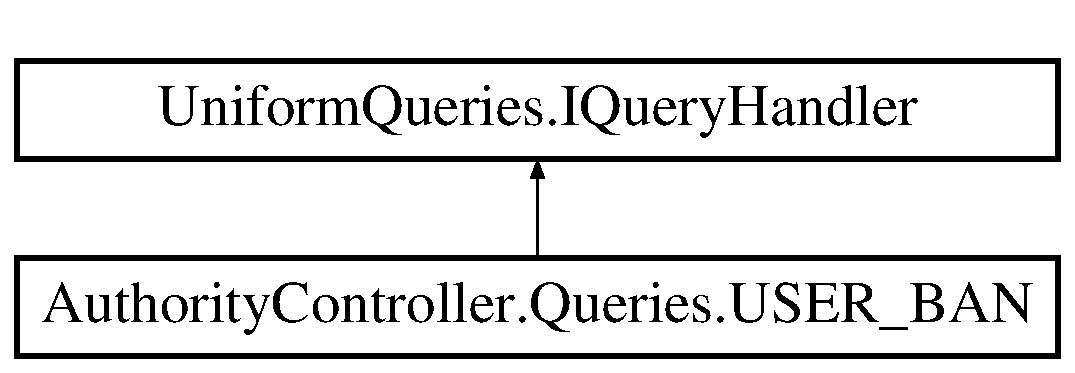
\includegraphics[height=2.000000cm]{d3/d4f/class_authority_controller_1_1_queries_1_1_u_s_e_r___b_a_n}
\end{center}
\end{figure}
\subsection*{Public Member Functions}
\begin{DoxyCompactItemize}
\item 
virtual string \mbox{\hyperlink{class_authority_controller_1_1_queries_1_1_u_s_e_r___b_a_n_ae0fe5998c22cf9fb76b601fbf7ee832e}{Description}} (string culture\+Key)
\begin{DoxyCompactList}\small\item\em Return the description relative to the lenguage code or default if not found. \end{DoxyCompactList}\item 
virtual void \mbox{\hyperlink{class_authority_controller_1_1_queries_1_1_u_s_e_r___b_a_n_a160a12bc99edf855a2bdddb908596ecf}{Execute}} (\mbox{\hyperlink{struct_uniform_queries_1_1_query_part}{Query\+Part}}\mbox{[}$\,$\mbox{]} query\+Parts)
\begin{DoxyCompactList}\small\item\em Methods that process query. \end{DoxyCompactList}\item 
virtual bool \mbox{\hyperlink{class_authority_controller_1_1_queries_1_1_u_s_e_r___b_a_n_a4f42625ac06de3292575a043ff0addd9}{Is\+Target}} (\mbox{\hyperlink{struct_uniform_queries_1_1_query_part}{Query\+Part}}\mbox{[}$\,$\mbox{]} query\+Parts)
\begin{DoxyCompactList}\small\item\em Check by the entry params does it target Query Handler. \end{DoxyCompactList}\end{DoxyCompactItemize}


\subsection{Detailed Description}
Set temporaly or permanent ban for user. 



\subsection{Member Function Documentation}
\mbox{\Hypertarget{class_authority_controller_1_1_queries_1_1_u_s_e_r___b_a_n_ae0fe5998c22cf9fb76b601fbf7ee832e}\label{class_authority_controller_1_1_queries_1_1_u_s_e_r___b_a_n_ae0fe5998c22cf9fb76b601fbf7ee832e}} 
\index{Authority\+Controller\+::\+Queries\+::\+U\+S\+E\+R\+\_\+\+B\+AN@{Authority\+Controller\+::\+Queries\+::\+U\+S\+E\+R\+\_\+\+B\+AN}!Description@{Description}}
\index{Description@{Description}!Authority\+Controller\+::\+Queries\+::\+U\+S\+E\+R\+\_\+\+B\+AN@{Authority\+Controller\+::\+Queries\+::\+U\+S\+E\+R\+\_\+\+B\+AN}}
\subsubsection{\texorpdfstring{Description()}{Description()}}
{\footnotesize\ttfamily virtual string Authority\+Controller.\+Queries.\+U\+S\+E\+R\+\_\+\+B\+A\+N.\+Description (\begin{DoxyParamCaption}\item[{string}]{culture\+Key }\end{DoxyParamCaption})\hspace{0.3cm}{\ttfamily [virtual]}}



Return the description relative to the lenguage code or default if not found. 


\begin{DoxyParams}{Parameters}
{\em culture\+Key} & \\
\hline
\end{DoxyParams}
\begin{DoxyReturn}{Returns}

\end{DoxyReturn}


Implements \mbox{\hyperlink{interface_uniform_queries_1_1_executable_1_1_i_query_handler_ae0e55919571d5456af31298394d241a9}{Uniform\+Queries.\+Executable.\+I\+Query\+Handler}}.

\mbox{\Hypertarget{class_authority_controller_1_1_queries_1_1_u_s_e_r___b_a_n_a160a12bc99edf855a2bdddb908596ecf}\label{class_authority_controller_1_1_queries_1_1_u_s_e_r___b_a_n_a160a12bc99edf855a2bdddb908596ecf}} 
\index{Authority\+Controller\+::\+Queries\+::\+U\+S\+E\+R\+\_\+\+B\+AN@{Authority\+Controller\+::\+Queries\+::\+U\+S\+E\+R\+\_\+\+B\+AN}!Execute@{Execute}}
\index{Execute@{Execute}!Authority\+Controller\+::\+Queries\+::\+U\+S\+E\+R\+\_\+\+B\+AN@{Authority\+Controller\+::\+Queries\+::\+U\+S\+E\+R\+\_\+\+B\+AN}}
\subsubsection{\texorpdfstring{Execute()}{Execute()}}
{\footnotesize\ttfamily virtual void Authority\+Controller.\+Queries.\+U\+S\+E\+R\+\_\+\+B\+A\+N.\+Execute (\begin{DoxyParamCaption}\item[{\mbox{\hyperlink{struct_uniform_queries_1_1_query_part}{Query\+Part}} \mbox{[}$\,$\mbox{]}}]{query\+Parts }\end{DoxyParamCaption})\hspace{0.3cm}{\ttfamily [virtual]}}



Methods that process query. 


\begin{DoxyParams}{Parameters}
{\em query\+Parts} & \\
\hline
\end{DoxyParams}


Implements \mbox{\hyperlink{interface_uniform_queries_1_1_executable_1_1_i_query_handler_a3268d72c0388f5e3debba4d73bdfe523}{Uniform\+Queries.\+Executable.\+I\+Query\+Handler}}.

\mbox{\Hypertarget{class_authority_controller_1_1_queries_1_1_u_s_e_r___b_a_n_a4f42625ac06de3292575a043ff0addd9}\label{class_authority_controller_1_1_queries_1_1_u_s_e_r___b_a_n_a4f42625ac06de3292575a043ff0addd9}} 
\index{Authority\+Controller\+::\+Queries\+::\+U\+S\+E\+R\+\_\+\+B\+AN@{Authority\+Controller\+::\+Queries\+::\+U\+S\+E\+R\+\_\+\+B\+AN}!Is\+Target@{Is\+Target}}
\index{Is\+Target@{Is\+Target}!Authority\+Controller\+::\+Queries\+::\+U\+S\+E\+R\+\_\+\+B\+AN@{Authority\+Controller\+::\+Queries\+::\+U\+S\+E\+R\+\_\+\+B\+AN}}
\subsubsection{\texorpdfstring{Is\+Target()}{IsTarget()}}
{\footnotesize\ttfamily virtual bool Authority\+Controller.\+Queries.\+U\+S\+E\+R\+\_\+\+B\+A\+N.\+Is\+Target (\begin{DoxyParamCaption}\item[{\mbox{\hyperlink{struct_uniform_queries_1_1_query_part}{Query\+Part}} \mbox{[}$\,$\mbox{]}}]{query\+Parts }\end{DoxyParamCaption})\hspace{0.3cm}{\ttfamily [virtual]}}



Check by the entry params does it target Query Handler. 


\begin{DoxyParams}{Parameters}
{\em query\+Parts} & \\
\hline
\end{DoxyParams}
\begin{DoxyReturn}{Returns}

\end{DoxyReturn}


Implements \mbox{\hyperlink{interface_uniform_queries_1_1_executable_1_1_i_query_handler_a0f43184bf3e306a7cbebc39098f044ee}{Uniform\+Queries.\+Executable.\+I\+Query\+Handler}}.



The documentation for this class was generated from the following file\+:\begin{DoxyCompactItemize}
\item 
D\+:/\+Work/\+Git\+Hub/doloro-\/networking-\/framework/\+Addons/\+Authority\+Controller/\+Queries/U\+S\+E\+R\+\_\+\+B\+A\+N.\+cs\end{DoxyCompactItemize}

\hypertarget{class_authority_controller_1_1_queries_1_1_u_s_e_r___l_o_g_o_f_f}{}\section{Authority\+Controller.\+Queries.\+U\+S\+E\+R\+\_\+\+L\+O\+G\+O\+FF Class Reference}
\label{class_authority_controller_1_1_queries_1_1_u_s_e_r___l_o_g_o_f_f}\index{Authority\+Controller.\+Queries.\+U\+S\+E\+R\+\_\+\+L\+O\+G\+O\+FF@{Authority\+Controller.\+Queries.\+U\+S\+E\+R\+\_\+\+L\+O\+G\+O\+FF}}


Log out user. Expire shared token.  


Inheritance diagram for Authority\+Controller.\+Queries.\+U\+S\+E\+R\+\_\+\+L\+O\+G\+O\+FF\+:\begin{figure}[H]
\begin{center}
\leavevmode
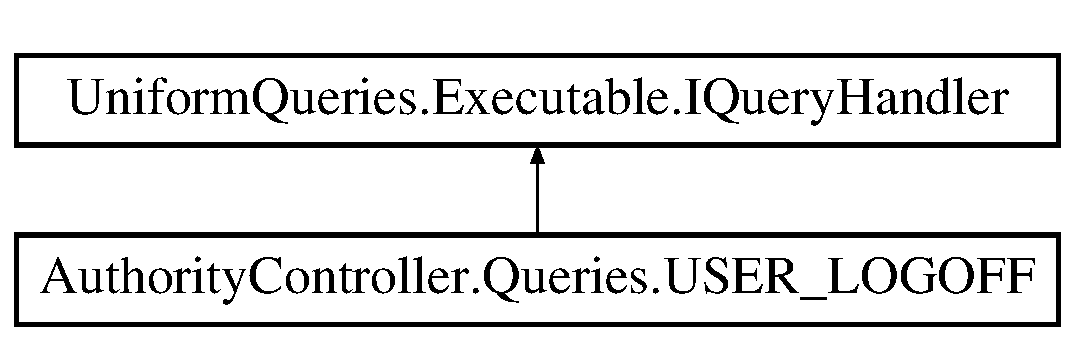
\includegraphics[height=2.000000cm]{db/d2a/class_authority_controller_1_1_queries_1_1_u_s_e_r___l_o_g_o_f_f}
\end{center}
\end{figure}
\subsection*{Public Member Functions}
\begin{DoxyCompactItemize}
\item 
string \mbox{\hyperlink{class_authority_controller_1_1_queries_1_1_u_s_e_r___l_o_g_o_f_f_a2cb738d74699241341b691cc55b57e1d}{Description}} (string culture\+Key)
\begin{DoxyCompactList}\small\item\em Return the description relative to the lenguage code or default if not found. \end{DoxyCompactList}\item 
void \mbox{\hyperlink{class_authority_controller_1_1_queries_1_1_u_s_e_r___l_o_g_o_f_f_a2e4d5a0f8ee93210522c41a38adbcce2}{Execute}} (\mbox{\hyperlink{struct_uniform_queries_1_1_query_part}{Query\+Part}}\mbox{[}$\,$\mbox{]} query\+Parts)
\begin{DoxyCompactList}\small\item\em Methods that process query. \end{DoxyCompactList}\item 
bool \mbox{\hyperlink{class_authority_controller_1_1_queries_1_1_u_s_e_r___l_o_g_o_f_f_afbfa78117d68ab2bd2728c78d31c1c58}{Is\+Target}} (\mbox{\hyperlink{struct_uniform_queries_1_1_query_part}{Query\+Part}}\mbox{[}$\,$\mbox{]} query\+Parts)
\begin{DoxyCompactList}\small\item\em Check by the entry params does it target Query Handler. \end{DoxyCompactList}\end{DoxyCompactItemize}
\subsection*{Static Public Member Functions}
\begin{DoxyCompactItemize}
\item 
static bool \mbox{\hyperlink{class_authority_controller_1_1_queries_1_1_u_s_e_r___l_o_g_o_f_f_aee1aba51496e1412706f77c53650955a}{Logoff\+Token}} (string token)
\begin{DoxyCompactList}\small\item\em Request token expiring that equal to logoff operation. \end{DoxyCompactList}\end{DoxyCompactItemize}


\subsection{Detailed Description}
Log out user. Expire shared token. 



\subsection{Member Function Documentation}
\mbox{\Hypertarget{class_authority_controller_1_1_queries_1_1_u_s_e_r___l_o_g_o_f_f_a2cb738d74699241341b691cc55b57e1d}\label{class_authority_controller_1_1_queries_1_1_u_s_e_r___l_o_g_o_f_f_a2cb738d74699241341b691cc55b57e1d}} 
\index{Authority\+Controller\+::\+Queries\+::\+U\+S\+E\+R\+\_\+\+L\+O\+G\+O\+FF@{Authority\+Controller\+::\+Queries\+::\+U\+S\+E\+R\+\_\+\+L\+O\+G\+O\+FF}!Description@{Description}}
\index{Description@{Description}!Authority\+Controller\+::\+Queries\+::\+U\+S\+E\+R\+\_\+\+L\+O\+G\+O\+FF@{Authority\+Controller\+::\+Queries\+::\+U\+S\+E\+R\+\_\+\+L\+O\+G\+O\+FF}}
\subsubsection{\texorpdfstring{Description()}{Description()}}
{\footnotesize\ttfamily string Authority\+Controller.\+Queries.\+U\+S\+E\+R\+\_\+\+L\+O\+G\+O\+F\+F.\+Description (\begin{DoxyParamCaption}\item[{string}]{culture\+Key }\end{DoxyParamCaption})}



Return the description relative to the lenguage code or default if not found. 


\begin{DoxyParams}{Parameters}
{\em culture\+Key} & \\
\hline
\end{DoxyParams}
\begin{DoxyReturn}{Returns}

\end{DoxyReturn}


Implements \mbox{\hyperlink{interface_uniform_queries_1_1_executable_1_1_i_query_handler_ae0e55919571d5456af31298394d241a9}{Uniform\+Queries.\+Executable.\+I\+Query\+Handler}}.

\mbox{\Hypertarget{class_authority_controller_1_1_queries_1_1_u_s_e_r___l_o_g_o_f_f_a2e4d5a0f8ee93210522c41a38adbcce2}\label{class_authority_controller_1_1_queries_1_1_u_s_e_r___l_o_g_o_f_f_a2e4d5a0f8ee93210522c41a38adbcce2}} 
\index{Authority\+Controller\+::\+Queries\+::\+U\+S\+E\+R\+\_\+\+L\+O\+G\+O\+FF@{Authority\+Controller\+::\+Queries\+::\+U\+S\+E\+R\+\_\+\+L\+O\+G\+O\+FF}!Execute@{Execute}}
\index{Execute@{Execute}!Authority\+Controller\+::\+Queries\+::\+U\+S\+E\+R\+\_\+\+L\+O\+G\+O\+FF@{Authority\+Controller\+::\+Queries\+::\+U\+S\+E\+R\+\_\+\+L\+O\+G\+O\+FF}}
\subsubsection{\texorpdfstring{Execute()}{Execute()}}
{\footnotesize\ttfamily void Authority\+Controller.\+Queries.\+U\+S\+E\+R\+\_\+\+L\+O\+G\+O\+F\+F.\+Execute (\begin{DoxyParamCaption}\item[{\mbox{\hyperlink{struct_uniform_queries_1_1_query_part}{Query\+Part}} \mbox{[}$\,$\mbox{]}}]{query\+Parts }\end{DoxyParamCaption})}



Methods that process query. 


\begin{DoxyParams}{Parameters}
{\em query\+Parts} & \\
\hline
\end{DoxyParams}


Implements \mbox{\hyperlink{interface_uniform_queries_1_1_executable_1_1_i_query_handler_a3268d72c0388f5e3debba4d73bdfe523}{Uniform\+Queries.\+Executable.\+I\+Query\+Handler}}.

\mbox{\Hypertarget{class_authority_controller_1_1_queries_1_1_u_s_e_r___l_o_g_o_f_f_afbfa78117d68ab2bd2728c78d31c1c58}\label{class_authority_controller_1_1_queries_1_1_u_s_e_r___l_o_g_o_f_f_afbfa78117d68ab2bd2728c78d31c1c58}} 
\index{Authority\+Controller\+::\+Queries\+::\+U\+S\+E\+R\+\_\+\+L\+O\+G\+O\+FF@{Authority\+Controller\+::\+Queries\+::\+U\+S\+E\+R\+\_\+\+L\+O\+G\+O\+FF}!Is\+Target@{Is\+Target}}
\index{Is\+Target@{Is\+Target}!Authority\+Controller\+::\+Queries\+::\+U\+S\+E\+R\+\_\+\+L\+O\+G\+O\+FF@{Authority\+Controller\+::\+Queries\+::\+U\+S\+E\+R\+\_\+\+L\+O\+G\+O\+FF}}
\subsubsection{\texorpdfstring{Is\+Target()}{IsTarget()}}
{\footnotesize\ttfamily bool Authority\+Controller.\+Queries.\+U\+S\+E\+R\+\_\+\+L\+O\+G\+O\+F\+F.\+Is\+Target (\begin{DoxyParamCaption}\item[{\mbox{\hyperlink{struct_uniform_queries_1_1_query_part}{Query\+Part}} \mbox{[}$\,$\mbox{]}}]{query\+Parts }\end{DoxyParamCaption})}



Check by the entry params does it target Query Handler. 


\begin{DoxyParams}{Parameters}
{\em query\+Parts} & \\
\hline
\end{DoxyParams}
\begin{DoxyReturn}{Returns}

\end{DoxyReturn}


Implements \mbox{\hyperlink{interface_uniform_queries_1_1_executable_1_1_i_query_handler_a0f43184bf3e306a7cbebc39098f044ee}{Uniform\+Queries.\+Executable.\+I\+Query\+Handler}}.

\mbox{\Hypertarget{class_authority_controller_1_1_queries_1_1_u_s_e_r___l_o_g_o_f_f_aee1aba51496e1412706f77c53650955a}\label{class_authority_controller_1_1_queries_1_1_u_s_e_r___l_o_g_o_f_f_aee1aba51496e1412706f77c53650955a}} 
\index{Authority\+Controller\+::\+Queries\+::\+U\+S\+E\+R\+\_\+\+L\+O\+G\+O\+FF@{Authority\+Controller\+::\+Queries\+::\+U\+S\+E\+R\+\_\+\+L\+O\+G\+O\+FF}!Logoff\+Token@{Logoff\+Token}}
\index{Logoff\+Token@{Logoff\+Token}!Authority\+Controller\+::\+Queries\+::\+U\+S\+E\+R\+\_\+\+L\+O\+G\+O\+FF@{Authority\+Controller\+::\+Queries\+::\+U\+S\+E\+R\+\_\+\+L\+O\+G\+O\+FF}}
\subsubsection{\texorpdfstring{Logoff\+Token()}{LogoffToken()}}
{\footnotesize\ttfamily static bool Authority\+Controller.\+Queries.\+U\+S\+E\+R\+\_\+\+L\+O\+G\+O\+F\+F.\+Logoff\+Token (\begin{DoxyParamCaption}\item[{string}]{token }\end{DoxyParamCaption})\hspace{0.3cm}{\ttfamily [static]}}



Request token expiring that equal to logoff operation. 


\begin{DoxyParams}{Parameters}
{\em token} & \\
\hline
\end{DoxyParams}


The documentation for this class was generated from the following file\+:\begin{DoxyCompactItemize}
\item 
D\+:/\+Work/\+Git\+Hub/doloro-\/networking-\/framework/\+Addons/\+Authority\+Controller/\+Queries/U\+S\+E\+R\+\_\+\+L\+O\+G\+O\+F\+F.\+cs\end{DoxyCompactItemize}

\hypertarget{class_authority_controller_1_1_queries_1_1_u_s_e_r___l_o_g_o_n}{}\section{Authority\+Controller.\+Queries.\+U\+S\+E\+R\+\_\+\+L\+O\+G\+ON Class Reference}
\label{class_authority_controller_1_1_queries_1_1_u_s_e_r___l_o_g_o_n}\index{Authority\+Controller.\+Queries.\+U\+S\+E\+R\+\_\+\+L\+O\+G\+ON@{Authority\+Controller.\+Queries.\+U\+S\+E\+R\+\_\+\+L\+O\+G\+ON}}


Logon user in system. Provide token as result.  


Inheritance diagram for Authority\+Controller.\+Queries.\+U\+S\+E\+R\+\_\+\+L\+O\+G\+ON\+:\begin{figure}[H]
\begin{center}
\leavevmode
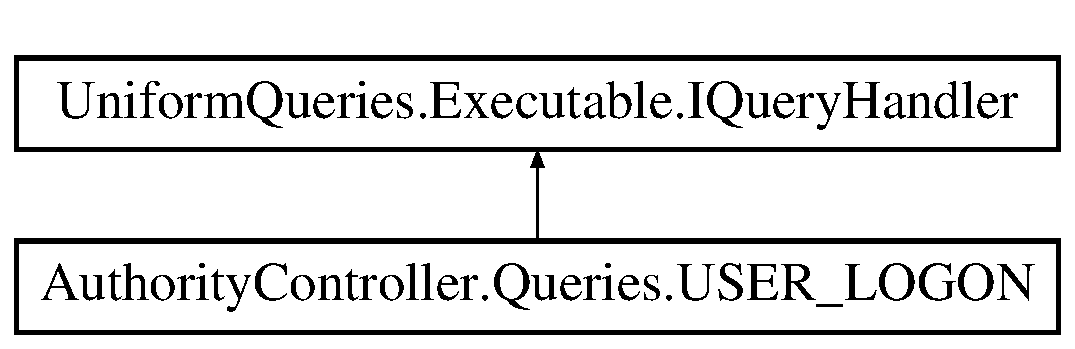
\includegraphics[height=2.000000cm]{de/d4c/class_authority_controller_1_1_queries_1_1_u_s_e_r___l_o_g_o_n}
\end{center}
\end{figure}
\subsection*{Public Member Functions}
\begin{DoxyCompactItemize}
\item 
string \mbox{\hyperlink{class_authority_controller_1_1_queries_1_1_u_s_e_r___l_o_g_o_n_af448426be46032c3ae103cdf4ea5f40b}{Description}} (string culture\+Key)
\begin{DoxyCompactList}\small\item\em Return the description relative to the lenguage code or default if not found. \end{DoxyCompactList}\item 
void \mbox{\hyperlink{class_authority_controller_1_1_queries_1_1_u_s_e_r___l_o_g_o_n_a001f81c71597259636be777078e50f7e}{Execute}} (\mbox{\hyperlink{struct_uniform_queries_1_1_query_part}{Query\+Part}}\mbox{[}$\,$\mbox{]} query\+Parts)
\begin{DoxyCompactList}\small\item\em Methods that process query. \end{DoxyCompactList}\item 
bool \mbox{\hyperlink{class_authority_controller_1_1_queries_1_1_u_s_e_r___l_o_g_o_n_a53261c6c60dc1a2324a67adf19f7547a}{Is\+Target}} (\mbox{\hyperlink{struct_uniform_queries_1_1_query_part}{Query\+Part}}\mbox{[}$\,$\mbox{]} query\+Parts)
\begin{DoxyCompactList}\small\item\em Check by the entry params does it target Query Handler. \end{DoxyCompactList}\end{DoxyCompactItemize}


\subsection{Detailed Description}
Logon user in system. Provide token as result. 

U\+S\+ER\&L\+O\+G\+ON\&login=...\&password=...\&mac=...\&os=....\& 

\subsection{Member Function Documentation}
\mbox{\Hypertarget{class_authority_controller_1_1_queries_1_1_u_s_e_r___l_o_g_o_n_af448426be46032c3ae103cdf4ea5f40b}\label{class_authority_controller_1_1_queries_1_1_u_s_e_r___l_o_g_o_n_af448426be46032c3ae103cdf4ea5f40b}} 
\index{Authority\+Controller\+::\+Queries\+::\+U\+S\+E\+R\+\_\+\+L\+O\+G\+ON@{Authority\+Controller\+::\+Queries\+::\+U\+S\+E\+R\+\_\+\+L\+O\+G\+ON}!Description@{Description}}
\index{Description@{Description}!Authority\+Controller\+::\+Queries\+::\+U\+S\+E\+R\+\_\+\+L\+O\+G\+ON@{Authority\+Controller\+::\+Queries\+::\+U\+S\+E\+R\+\_\+\+L\+O\+G\+ON}}
\subsubsection{\texorpdfstring{Description()}{Description()}}
{\footnotesize\ttfamily string Authority\+Controller.\+Queries.\+U\+S\+E\+R\+\_\+\+L\+O\+G\+O\+N.\+Description (\begin{DoxyParamCaption}\item[{string}]{culture\+Key }\end{DoxyParamCaption})}



Return the description relative to the lenguage code or default if not found. 


\begin{DoxyParams}{Parameters}
{\em culture\+Key} & \\
\hline
\end{DoxyParams}
\begin{DoxyReturn}{Returns}

\end{DoxyReturn}


Implements \mbox{\hyperlink{interface_uniform_queries_1_1_i_query_handler_abe2d1124630ca8d74b7398d11c873526}{Uniform\+Queries.\+I\+Query\+Handler}}.

\mbox{\Hypertarget{class_authority_controller_1_1_queries_1_1_u_s_e_r___l_o_g_o_n_a001f81c71597259636be777078e50f7e}\label{class_authority_controller_1_1_queries_1_1_u_s_e_r___l_o_g_o_n_a001f81c71597259636be777078e50f7e}} 
\index{Authority\+Controller\+::\+Queries\+::\+U\+S\+E\+R\+\_\+\+L\+O\+G\+ON@{Authority\+Controller\+::\+Queries\+::\+U\+S\+E\+R\+\_\+\+L\+O\+G\+ON}!Execute@{Execute}}
\index{Execute@{Execute}!Authority\+Controller\+::\+Queries\+::\+U\+S\+E\+R\+\_\+\+L\+O\+G\+ON@{Authority\+Controller\+::\+Queries\+::\+U\+S\+E\+R\+\_\+\+L\+O\+G\+ON}}
\subsubsection{\texorpdfstring{Execute()}{Execute()}}
{\footnotesize\ttfamily void Authority\+Controller.\+Queries.\+U\+S\+E\+R\+\_\+\+L\+O\+G\+O\+N.\+Execute (\begin{DoxyParamCaption}\item[{\mbox{\hyperlink{struct_uniform_queries_1_1_query_part}{Query\+Part}} \mbox{[}$\,$\mbox{]}}]{query\+Parts }\end{DoxyParamCaption})}



Methods that process query. 


\begin{DoxyParams}{Parameters}
{\em query\+Parts} & \\
\hline
\end{DoxyParams}


Implements \mbox{\hyperlink{interface_uniform_queries_1_1_i_query_handler_a66d15db03bdd5b0caf6eef96f9b803c0}{Uniform\+Queries.\+I\+Query\+Handler}}.

\mbox{\Hypertarget{class_authority_controller_1_1_queries_1_1_u_s_e_r___l_o_g_o_n_a53261c6c60dc1a2324a67adf19f7547a}\label{class_authority_controller_1_1_queries_1_1_u_s_e_r___l_o_g_o_n_a53261c6c60dc1a2324a67adf19f7547a}} 
\index{Authority\+Controller\+::\+Queries\+::\+U\+S\+E\+R\+\_\+\+L\+O\+G\+ON@{Authority\+Controller\+::\+Queries\+::\+U\+S\+E\+R\+\_\+\+L\+O\+G\+ON}!Is\+Target@{Is\+Target}}
\index{Is\+Target@{Is\+Target}!Authority\+Controller\+::\+Queries\+::\+U\+S\+E\+R\+\_\+\+L\+O\+G\+ON@{Authority\+Controller\+::\+Queries\+::\+U\+S\+E\+R\+\_\+\+L\+O\+G\+ON}}
\subsubsection{\texorpdfstring{Is\+Target()}{IsTarget()}}
{\footnotesize\ttfamily bool Authority\+Controller.\+Queries.\+U\+S\+E\+R\+\_\+\+L\+O\+G\+O\+N.\+Is\+Target (\begin{DoxyParamCaption}\item[{\mbox{\hyperlink{struct_uniform_queries_1_1_query_part}{Query\+Part}} \mbox{[}$\,$\mbox{]}}]{query\+Parts }\end{DoxyParamCaption})}



Check by the entry params does it target Query Handler. 


\begin{DoxyParams}{Parameters}
{\em query\+Parts} & \\
\hline
\end{DoxyParams}
\begin{DoxyReturn}{Returns}

\end{DoxyReturn}


Implements \mbox{\hyperlink{interface_uniform_queries_1_1_i_query_handler_abda1ccf47ad2889fbd015955965046e7}{Uniform\+Queries.\+I\+Query\+Handler}}.



The documentation for this class was generated from the following file\+:\begin{DoxyCompactItemize}
\item 
D\+:/\+Work/\+Git\+Hub/doloro-\/networking-\/framework/\+Authority\+Controller/\+Queries/U\+S\+E\+R\+\_\+\+L\+O\+G\+O\+N.\+cs\end{DoxyCompactItemize}

\hypertarget{class_authority_controller_1_1_queries_1_1_u_s_e_r___n_e_w}{}\section{Authority\+Controller.\+Queries.\+U\+S\+E\+R\+\_\+\+N\+EW Class Reference}
\label{class_authority_controller_1_1_queries_1_1_u_s_e_r___n_e_w}\index{Authority\+Controller.\+Queries.\+U\+S\+E\+R\+\_\+\+N\+EW@{Authority\+Controller.\+Queries.\+U\+S\+E\+R\+\_\+\+N\+EW}}


Create new user.  


Inheritance diagram for Authority\+Controller.\+Queries.\+U\+S\+E\+R\+\_\+\+N\+EW\+:\begin{figure}[H]
\begin{center}
\leavevmode
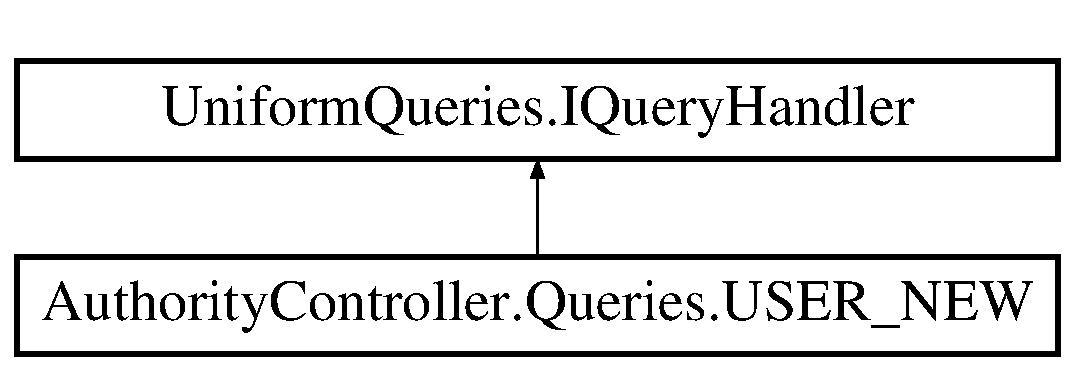
\includegraphics[height=2.000000cm]{d1/d07/class_authority_controller_1_1_queries_1_1_u_s_e_r___n_e_w}
\end{center}
\end{figure}
\subsection*{Public Member Functions}
\begin{DoxyCompactItemize}
\item 
string \mbox{\hyperlink{class_authority_controller_1_1_queries_1_1_u_s_e_r___n_e_w_ab0995d0559e0033ea963acaccb6e37bf}{Description}} (string culture\+Key)
\begin{DoxyCompactList}\small\item\em Return the description relative to the lenguage code or default if not found. \end{DoxyCompactList}\item 
void \mbox{\hyperlink{class_authority_controller_1_1_queries_1_1_u_s_e_r___n_e_w_afd715fb3d60e53ca7e3d55a4433f529c}{Execute}} (\mbox{\hyperlink{struct_uniform_queries_1_1_query_part}{Query\+Part}}\mbox{[}$\,$\mbox{]} query\+Parts)
\begin{DoxyCompactList}\small\item\em Methods that process query. \end{DoxyCompactList}\item 
bool \mbox{\hyperlink{class_authority_controller_1_1_queries_1_1_u_s_e_r___n_e_w_a6e26596b5a5ecc3d07591766b5d325ec}{Is\+Target}} (\mbox{\hyperlink{struct_uniform_queries_1_1_query_part}{Query\+Part}}\mbox{[}$\,$\mbox{]} query\+Parts)
\begin{DoxyCompactList}\small\item\em Check by the entry params does it target Query Handler. \end{DoxyCompactList}\end{DoxyCompactItemize}


\subsection{Detailed Description}
Create new user. 



\subsection{Member Function Documentation}
\mbox{\Hypertarget{class_authority_controller_1_1_queries_1_1_u_s_e_r___n_e_w_ab0995d0559e0033ea963acaccb6e37bf}\label{class_authority_controller_1_1_queries_1_1_u_s_e_r___n_e_w_ab0995d0559e0033ea963acaccb6e37bf}} 
\index{Authority\+Controller\+::\+Queries\+::\+U\+S\+E\+R\+\_\+\+N\+EW@{Authority\+Controller\+::\+Queries\+::\+U\+S\+E\+R\+\_\+\+N\+EW}!Description@{Description}}
\index{Description@{Description}!Authority\+Controller\+::\+Queries\+::\+U\+S\+E\+R\+\_\+\+N\+EW@{Authority\+Controller\+::\+Queries\+::\+U\+S\+E\+R\+\_\+\+N\+EW}}
\subsubsection{\texorpdfstring{Description()}{Description()}}
{\footnotesize\ttfamily string Authority\+Controller.\+Queries.\+U\+S\+E\+R\+\_\+\+N\+E\+W.\+Description (\begin{DoxyParamCaption}\item[{string}]{culture\+Key }\end{DoxyParamCaption})}



Return the description relative to the lenguage code or default if not found. 


\begin{DoxyParams}{Parameters}
{\em culture\+Key} & \\
\hline
\end{DoxyParams}
\begin{DoxyReturn}{Returns}

\end{DoxyReturn}


Implements \mbox{\hyperlink{interface_uniform_queries_1_1_i_query_handler_abe2d1124630ca8d74b7398d11c873526}{Uniform\+Queries.\+I\+Query\+Handler}}.

\mbox{\Hypertarget{class_authority_controller_1_1_queries_1_1_u_s_e_r___n_e_w_afd715fb3d60e53ca7e3d55a4433f529c}\label{class_authority_controller_1_1_queries_1_1_u_s_e_r___n_e_w_afd715fb3d60e53ca7e3d55a4433f529c}} 
\index{Authority\+Controller\+::\+Queries\+::\+U\+S\+E\+R\+\_\+\+N\+EW@{Authority\+Controller\+::\+Queries\+::\+U\+S\+E\+R\+\_\+\+N\+EW}!Execute@{Execute}}
\index{Execute@{Execute}!Authority\+Controller\+::\+Queries\+::\+U\+S\+E\+R\+\_\+\+N\+EW@{Authority\+Controller\+::\+Queries\+::\+U\+S\+E\+R\+\_\+\+N\+EW}}
\subsubsection{\texorpdfstring{Execute()}{Execute()}}
{\footnotesize\ttfamily void Authority\+Controller.\+Queries.\+U\+S\+E\+R\+\_\+\+N\+E\+W.\+Execute (\begin{DoxyParamCaption}\item[{\mbox{\hyperlink{struct_uniform_queries_1_1_query_part}{Query\+Part}} \mbox{[}$\,$\mbox{]}}]{query\+Parts }\end{DoxyParamCaption})}



Methods that process query. 


\begin{DoxyParams}{Parameters}
{\em query\+Parts} & \\
\hline
\end{DoxyParams}


Implements \mbox{\hyperlink{interface_uniform_queries_1_1_i_query_handler_a66d15db03bdd5b0caf6eef96f9b803c0}{Uniform\+Queries.\+I\+Query\+Handler}}.

\mbox{\Hypertarget{class_authority_controller_1_1_queries_1_1_u_s_e_r___n_e_w_a6e26596b5a5ecc3d07591766b5d325ec}\label{class_authority_controller_1_1_queries_1_1_u_s_e_r___n_e_w_a6e26596b5a5ecc3d07591766b5d325ec}} 
\index{Authority\+Controller\+::\+Queries\+::\+U\+S\+E\+R\+\_\+\+N\+EW@{Authority\+Controller\+::\+Queries\+::\+U\+S\+E\+R\+\_\+\+N\+EW}!Is\+Target@{Is\+Target}}
\index{Is\+Target@{Is\+Target}!Authority\+Controller\+::\+Queries\+::\+U\+S\+E\+R\+\_\+\+N\+EW@{Authority\+Controller\+::\+Queries\+::\+U\+S\+E\+R\+\_\+\+N\+EW}}
\subsubsection{\texorpdfstring{Is\+Target()}{IsTarget()}}
{\footnotesize\ttfamily bool Authority\+Controller.\+Queries.\+U\+S\+E\+R\+\_\+\+N\+E\+W.\+Is\+Target (\begin{DoxyParamCaption}\item[{\mbox{\hyperlink{struct_uniform_queries_1_1_query_part}{Query\+Part}} \mbox{[}$\,$\mbox{]}}]{query\+Parts }\end{DoxyParamCaption})}



Check by the entry params does it target Query Handler. 


\begin{DoxyParams}{Parameters}
{\em query\+Parts} & \\
\hline
\end{DoxyParams}
\begin{DoxyReturn}{Returns}

\end{DoxyReturn}


Implements \mbox{\hyperlink{interface_uniform_queries_1_1_i_query_handler_abda1ccf47ad2889fbd015955965046e7}{Uniform\+Queries.\+I\+Query\+Handler}}.



The documentation for this class was generated from the following file\+:\begin{DoxyCompactItemize}
\item 
D\+:/\+Work/\+Git\+Hub/doloro-\/networking-\/framework/\+Authority\+Controller/\+Queries/U\+S\+E\+R\+\_\+\+N\+E\+W.\+cs\end{DoxyCompactItemize}

\hypertarget{class_authority_controller_1_1_queries_1_1_u_s_e_r___n_e_w___p_a_s_s_w_o_r_d}{}\section{Authority\+Controller.\+Queries.\+U\+S\+E\+R\+\_\+\+N\+E\+W\+\_\+\+P\+A\+S\+S\+W\+O\+RD Class Reference}
\label{class_authority_controller_1_1_queries_1_1_u_s_e_r___n_e_w___p_a_s_s_w_o_r_d}\index{Authority\+Controller.\+Queries.\+U\+S\+E\+R\+\_\+\+N\+E\+W\+\_\+\+P\+A\+S\+S\+W\+O\+RD@{Authority\+Controller.\+Queries.\+U\+S\+E\+R\+\_\+\+N\+E\+W\+\_\+\+P\+A\+S\+S\+W\+O\+RD}}


Set new password for user. Require admin or certen user rights.  


Inheritance diagram for Authority\+Controller.\+Queries.\+U\+S\+E\+R\+\_\+\+N\+E\+W\+\_\+\+P\+A\+S\+S\+W\+O\+RD\+:\begin{figure}[H]
\begin{center}
\leavevmode
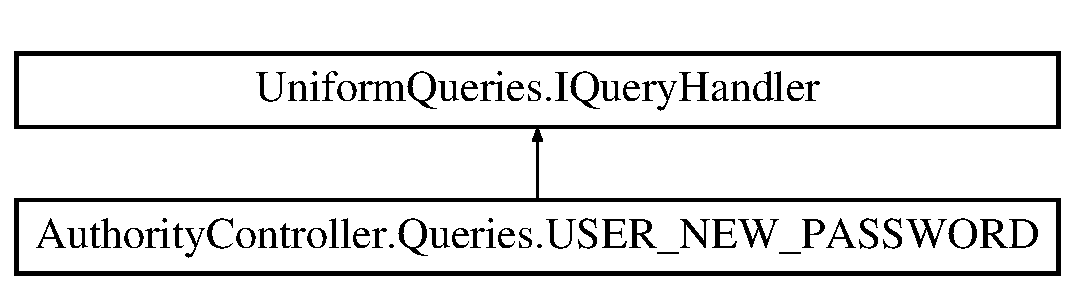
\includegraphics[height=2.000000cm]{d5/d21/class_authority_controller_1_1_queries_1_1_u_s_e_r___n_e_w___p_a_s_s_w_o_r_d}
\end{center}
\end{figure}
\subsection*{Public Member Functions}
\begin{DoxyCompactItemize}
\item 
string \mbox{\hyperlink{class_authority_controller_1_1_queries_1_1_u_s_e_r___n_e_w___p_a_s_s_w_o_r_d_a04d2af1732d4ac353076d489fe75c696}{Description}} (string culture\+Key)
\begin{DoxyCompactList}\small\item\em Return the description relative to the lenguage code or default if not found. \end{DoxyCompactList}\item 
void \mbox{\hyperlink{class_authority_controller_1_1_queries_1_1_u_s_e_r___n_e_w___p_a_s_s_w_o_r_d_a63a5424c90f45f09f72a530ef0389416}{Execute}} (\mbox{\hyperlink{struct_uniform_queries_1_1_query_part}{Query\+Part}}\mbox{[}$\,$\mbox{]} query\+Parts)
\begin{DoxyCompactList}\small\item\em Methods that process query. \end{DoxyCompactList}\item 
bool \mbox{\hyperlink{class_authority_controller_1_1_queries_1_1_u_s_e_r___n_e_w___p_a_s_s_w_o_r_d_a48ff6874453caf45973ad386bfe5b513}{Is\+Target}} (\mbox{\hyperlink{struct_uniform_queries_1_1_query_part}{Query\+Part}}\mbox{[}$\,$\mbox{]} query\+Parts)
\begin{DoxyCompactList}\small\item\em Check by the entry params does it target Query Handler. \end{DoxyCompactList}\end{DoxyCompactItemize}


\subsection{Detailed Description}
Set new password for user. Require admin or certen user rights. 



\subsection{Member Function Documentation}
\mbox{\Hypertarget{class_authority_controller_1_1_queries_1_1_u_s_e_r___n_e_w___p_a_s_s_w_o_r_d_a04d2af1732d4ac353076d489fe75c696}\label{class_authority_controller_1_1_queries_1_1_u_s_e_r___n_e_w___p_a_s_s_w_o_r_d_a04d2af1732d4ac353076d489fe75c696}} 
\index{Authority\+Controller\+::\+Queries\+::\+U\+S\+E\+R\+\_\+\+N\+E\+W\+\_\+\+P\+A\+S\+S\+W\+O\+RD@{Authority\+Controller\+::\+Queries\+::\+U\+S\+E\+R\+\_\+\+N\+E\+W\+\_\+\+P\+A\+S\+S\+W\+O\+RD}!Description@{Description}}
\index{Description@{Description}!Authority\+Controller\+::\+Queries\+::\+U\+S\+E\+R\+\_\+\+N\+E\+W\+\_\+\+P\+A\+S\+S\+W\+O\+RD@{Authority\+Controller\+::\+Queries\+::\+U\+S\+E\+R\+\_\+\+N\+E\+W\+\_\+\+P\+A\+S\+S\+W\+O\+RD}}
\subsubsection{\texorpdfstring{Description()}{Description()}}
{\footnotesize\ttfamily string Authority\+Controller.\+Queries.\+U\+S\+E\+R\+\_\+\+N\+E\+W\+\_\+\+P\+A\+S\+S\+W\+O\+R\+D.\+Description (\begin{DoxyParamCaption}\item[{string}]{culture\+Key }\end{DoxyParamCaption})}



Return the description relative to the lenguage code or default if not found. 


\begin{DoxyParams}{Parameters}
{\em culture\+Key} & \\
\hline
\end{DoxyParams}
\begin{DoxyReturn}{Returns}

\end{DoxyReturn}


Implements \mbox{\hyperlink{interface_uniform_queries_1_1_executable_1_1_i_query_handler_ae0e55919571d5456af31298394d241a9}{Uniform\+Queries.\+Executable.\+I\+Query\+Handler}}.

\mbox{\Hypertarget{class_authority_controller_1_1_queries_1_1_u_s_e_r___n_e_w___p_a_s_s_w_o_r_d_a63a5424c90f45f09f72a530ef0389416}\label{class_authority_controller_1_1_queries_1_1_u_s_e_r___n_e_w___p_a_s_s_w_o_r_d_a63a5424c90f45f09f72a530ef0389416}} 
\index{Authority\+Controller\+::\+Queries\+::\+U\+S\+E\+R\+\_\+\+N\+E\+W\+\_\+\+P\+A\+S\+S\+W\+O\+RD@{Authority\+Controller\+::\+Queries\+::\+U\+S\+E\+R\+\_\+\+N\+E\+W\+\_\+\+P\+A\+S\+S\+W\+O\+RD}!Execute@{Execute}}
\index{Execute@{Execute}!Authority\+Controller\+::\+Queries\+::\+U\+S\+E\+R\+\_\+\+N\+E\+W\+\_\+\+P\+A\+S\+S\+W\+O\+RD@{Authority\+Controller\+::\+Queries\+::\+U\+S\+E\+R\+\_\+\+N\+E\+W\+\_\+\+P\+A\+S\+S\+W\+O\+RD}}
\subsubsection{\texorpdfstring{Execute()}{Execute()}}
{\footnotesize\ttfamily void Authority\+Controller.\+Queries.\+U\+S\+E\+R\+\_\+\+N\+E\+W\+\_\+\+P\+A\+S\+S\+W\+O\+R\+D.\+Execute (\begin{DoxyParamCaption}\item[{\mbox{\hyperlink{struct_uniform_queries_1_1_query_part}{Query\+Part}} \mbox{[}$\,$\mbox{]}}]{query\+Parts }\end{DoxyParamCaption})}



Methods that process query. 


\begin{DoxyParams}{Parameters}
{\em query\+Parts} & \\
\hline
\end{DoxyParams}


Implements \mbox{\hyperlink{interface_uniform_queries_1_1_executable_1_1_i_query_handler_a3268d72c0388f5e3debba4d73bdfe523}{Uniform\+Queries.\+Executable.\+I\+Query\+Handler}}.

\mbox{\Hypertarget{class_authority_controller_1_1_queries_1_1_u_s_e_r___n_e_w___p_a_s_s_w_o_r_d_a48ff6874453caf45973ad386bfe5b513}\label{class_authority_controller_1_1_queries_1_1_u_s_e_r___n_e_w___p_a_s_s_w_o_r_d_a48ff6874453caf45973ad386bfe5b513}} 
\index{Authority\+Controller\+::\+Queries\+::\+U\+S\+E\+R\+\_\+\+N\+E\+W\+\_\+\+P\+A\+S\+S\+W\+O\+RD@{Authority\+Controller\+::\+Queries\+::\+U\+S\+E\+R\+\_\+\+N\+E\+W\+\_\+\+P\+A\+S\+S\+W\+O\+RD}!Is\+Target@{Is\+Target}}
\index{Is\+Target@{Is\+Target}!Authority\+Controller\+::\+Queries\+::\+U\+S\+E\+R\+\_\+\+N\+E\+W\+\_\+\+P\+A\+S\+S\+W\+O\+RD@{Authority\+Controller\+::\+Queries\+::\+U\+S\+E\+R\+\_\+\+N\+E\+W\+\_\+\+P\+A\+S\+S\+W\+O\+RD}}
\subsubsection{\texorpdfstring{Is\+Target()}{IsTarget()}}
{\footnotesize\ttfamily bool Authority\+Controller.\+Queries.\+U\+S\+E\+R\+\_\+\+N\+E\+W\+\_\+\+P\+A\+S\+S\+W\+O\+R\+D.\+Is\+Target (\begin{DoxyParamCaption}\item[{\mbox{\hyperlink{struct_uniform_queries_1_1_query_part}{Query\+Part}} \mbox{[}$\,$\mbox{]}}]{query\+Parts }\end{DoxyParamCaption})}



Check by the entry params does it target Query Handler. 


\begin{DoxyParams}{Parameters}
{\em query\+Parts} & \\
\hline
\end{DoxyParams}
\begin{DoxyReturn}{Returns}

\end{DoxyReturn}


Implements \mbox{\hyperlink{interface_uniform_queries_1_1_executable_1_1_i_query_handler_a0f43184bf3e306a7cbebc39098f044ee}{Uniform\+Queries.\+Executable.\+I\+Query\+Handler}}.



The documentation for this class was generated from the following file\+:\begin{DoxyCompactItemize}
\item 
D\+:/\+Work/\+Git\+Hub/doloro-\/networking-\/framework/\+Addons/\+Authority\+Controller/\+Queries/U\+S\+E\+R\+\_\+\+N\+E\+W\+\_\+\+P\+A\+S\+S\+W\+O\+R\+D.\+cs\end{DoxyCompactItemize}

\hypertarget{class_authority_controller_1_1_a_p_i_1_1_validation}{}\section{Authority\+Controller.\+A\+P\+I.\+Validation Class Reference}
\label{class_authority_controller_1_1_a_p_i_1_1_validation}\index{Authority\+Controller.\+A\+P\+I.\+Validation@{Authority\+Controller.\+A\+P\+I.\+Validation}}
\subsection*{Static Public Member Functions}
\begin{DoxyCompactItemize}
\item 
static bool \mbox{\hyperlink{class_authority_controller_1_1_a_p_i_1_1_validation_a9aceff242f489e5d63808e28b1506487}{Password\+Format}} (string password, out string error)
\begin{DoxyCompactList}\small\item\em Validate password before converting to salted hash. \end{DoxyCompactList}\item 
static bool \mbox{\hyperlink{class_authority_controller_1_1_a_p_i_1_1_validation_a105196c0f8ec27b96594e2ac855b7db3}{Name\+Format}} (ref string name\+Part, out string error)
\begin{DoxyCompactList}\small\item\em Validate name part format. \end{DoxyCompactList}\end{DoxyCompactItemize}


\subsection{Member Function Documentation}
\mbox{\Hypertarget{class_authority_controller_1_1_a_p_i_1_1_validation_a105196c0f8ec27b96594e2ac855b7db3}\label{class_authority_controller_1_1_a_p_i_1_1_validation_a105196c0f8ec27b96594e2ac855b7db3}} 
\index{Authority\+Controller\+::\+A\+P\+I\+::\+Validation@{Authority\+Controller\+::\+A\+P\+I\+::\+Validation}!Name\+Format@{Name\+Format}}
\index{Name\+Format@{Name\+Format}!Authority\+Controller\+::\+A\+P\+I\+::\+Validation@{Authority\+Controller\+::\+A\+P\+I\+::\+Validation}}
\subsubsection{\texorpdfstring{Name\+Format()}{NameFormat()}}
{\footnotesize\ttfamily static bool Authority\+Controller.\+A\+P\+I.\+Validation.\+Name\+Format (\begin{DoxyParamCaption}\item[{ref string}]{name\+Part,  }\item[{out string}]{error }\end{DoxyParamCaption})\hspace{0.3cm}{\ttfamily [static]}}



Validate name part format. 


\begin{DoxyParams}{Parameters}
{\em name\+Part} & First part of the name that need to be validated\\
\hline
{\em error} & Error string that will be situable in case of validation fail.\\
\hline
\end{DoxyParams}
\begin{DoxyReturn}{Returns}
Result of validation.
\end{DoxyReturn}
\mbox{\Hypertarget{class_authority_controller_1_1_a_p_i_1_1_validation_a9aceff242f489e5d63808e28b1506487}\label{class_authority_controller_1_1_a_p_i_1_1_validation_a9aceff242f489e5d63808e28b1506487}} 
\index{Authority\+Controller\+::\+A\+P\+I\+::\+Validation@{Authority\+Controller\+::\+A\+P\+I\+::\+Validation}!Password\+Format@{Password\+Format}}
\index{Password\+Format@{Password\+Format}!Authority\+Controller\+::\+A\+P\+I\+::\+Validation@{Authority\+Controller\+::\+A\+P\+I\+::\+Validation}}
\subsubsection{\texorpdfstring{Password\+Format()}{PasswordFormat()}}
{\footnotesize\ttfamily static bool Authority\+Controller.\+A\+P\+I.\+Validation.\+Password\+Format (\begin{DoxyParamCaption}\item[{string}]{password,  }\item[{out string}]{error }\end{DoxyParamCaption})\hspace{0.3cm}{\ttfamily [static]}}



Validate password before converting to salted hash. 


\begin{DoxyParams}{Parameters}
{\em password} & Open password.\\
\hline
{\em error} & Error string that will be situable in case of validation fail.\\
\hline
\end{DoxyParams}
\begin{DoxyReturn}{Returns}
Result of validation.
\end{DoxyReturn}


The documentation for this class was generated from the following file\+:\begin{DoxyCompactItemize}
\item 
D\+:/\+Work/\+Git\+Hub/doloro-\/networking-\/framework/\+Addons/\+Authority\+Controller/\+A\+P\+I/Validation.\+cs\end{DoxyCompactItemize}

%--- End generated contents ---

% Index
\backmatter
\newpage
\phantomsection
\clearemptydoublepage
\addcontentsline{toc}{chapter}{Index}
\printindex

\end{document}
